\documentclass{article}

\usepackage[latin1]{inputenc}
\usepackage[T1]{fontenc}
\usepackage{makeidx}
\usepackage{latexsym}
\usepackage{verbatim}
\usepackage{moreverb}
\usepackage{index}
\usepackage{dingbat}
\usepackage{fancyhdr}

\usepackage{ifpdf}

% \newif\ifpdf
% \ifx\pdfoutput\undefined
% \else
%   \ifx\pdfoutput\relax
%   \else
%     \ifcase\pdfoutput
%     \else
%       \pdftrue
%     \fi
%   \fi
% \fi
\ifpdf
  \usepackage[pdftex,colorlinks=true,bookmarksopen, pdfstartview=FitH,
              linkcolor=blue, citecolor=blue, urlcolor=blue]{hyperref}
  \usepackage[pdftex]{graphicx}
  \pdfcompresslevel=9
\else
  \usepackage[dvips]{graphicx}
\fi

\usepackage{ae}
\usepackage{aecompl}

% ----------------------------------------------------------------
% HORIZONTAL MARGINS
% Left margin, odd pages: 1.25 inch (0.25 + 1)
\setlength{\oddsidemargin}{0.25in}
% Left margin, even pages: 1.25 inch (0 + 1)
\setlength{\evensidemargin}{0.25in}
% Text width 6 inch (so other margin is 1.25 inch).
\setlength{\textwidth}{6in}
% ----------------
% VERTICAL MARGINS
% Top margin 0.5 inch (-0.5 + 1)
\setlength{\topmargin}{-0.5in}
% Head height 0.25 inch (where page headers go)
\setlength{\headheight}{0.25in}
% Head separation 0.25 inch (between header and top line of text)
\setlength{\headsep}{0.25in}
% Text height 9 inch (so bottom margin 1 in)
\setlength{\textheight}{9in}
% ----------------
% PARAGRAPH INDENTATION
\setlength{\parindent}{0in}
% SPACE BETWEEN PARAGRAPHS
\setlength{\parskip}{\medskipamount}
% ----------------
% STRUTS
% HORIZONTAL STRUT.  One argument (width).
\newcommand{\hstrut}[1]{\hspace*{#1}}
% VERTICAL STRUT. Two arguments (offset from baseline, height).
\newcommand{\vstrut}[2]{\rule[#1]{0in}{#2}}
% ----------------
% HORIZONTAL LINE ACROSS PAGE:
\newcommand{\hdivider}{\noindent\mbox{}\hrulefill\mbox{}} 
% ----------------
% EMPTY BOXES OF VARIOUS WIDTHS, FOR INDENTATION
\newcommand{\hm}{\hspace*{1em}}
\newcommand{\hmm}{\hspace*{2em}}
\newcommand{\hmmm}{\hspace*{3em}}
\newcommand{\hmmmm}{\hspace*{4em}}
% ----------------
% ``TIGHTLIST'' ENVIRONMENT (no para space betwee items, small indent)
\newenvironment{tightlist}%
{\begin{list}{$\bullet$}{%
    \setlength{\topsep}{0in}
    \setlength{\partopsep}{0in}
    \setlength{\itemsep}{0in}
    \setlength{\parsep}{0in}
    \setlength{\leftmargin}{1.5em}
    \setlength{\rightmargin}{0in}
    \setlength{\itemindent}{0in}
}
}%
{\end{list}
}

%----------------
% Added to get special characters in index
\newcommand{\Caret}{\char94}
\newcommand{\Tilde}{\char126}


% ----------------
% Language names

% Name for the company
\newcommand{\BS}{Bluespec}
% Name for the languages and tools
\newcommand{\Blue}{Bluespec}

\newcommand{\BSV}{BSV}
\newcommand{\BSVFull}{Bluespec SystemVerilog}

\newcommand{\BH}{BH}
\newcommand{\BHFull}{Bluespec Haskell/Classic}

\newcommand{\V}{Verilog}
\newcommand{\veri}{Verilog}

% ----------------------------------------------------------------
% CODE DISPLAYS.
% Bluespec code displays are enclosed between \BBS and \EBS
% Most characters are taken verbatim, in typewriter font,
% Except:
%  Commands are still available (beginning with \)
%    but use ` and ' instead of { and }
%  Math mode is still available (beginning with $)
%    but use ~ and ! for ^ and _

\outer\def\BBS{%
  \begin{list}{$\bullet$}{%
    \setlength{\topsep}{0in}
    \setlength{\partopsep}{0in}
    \setlength{\itemsep}{0in}
    \setlength{\parsep}{0in}
    \setlength{\leftmargin}{1em}
    \setlength{\rightmargin}{0in}
    \setlength{\itemindent}{0in}
  }\item[]
%  \catcode`\{=12
%  \catcode`\}=12
  \catcode`\&=12
  \catcode`\#=12
  \catcode`\%=12
  \catcode`\~=12
%  \catcode`\_=12
  \catcode`\^=12
%  \catcode`\~=7
%  \catcode`\!=7      % superscript
%  \catcode`\'=2
%  \catcode`\`=1
  \obeyspaces
  \obeylines \tt}

\outer\def\EBS{%
  \end{list}
  }

{\obeyspaces\gdef {\ }}

% ----------------------------------------------------------------
% The following hack is from Mark Tuttle
\newcommand{\ttsymbol}[1]{%
  % print character at position #1 in the tt font family in current font size
  \begingroup\fontfamily{cmtt}\selectfont\symbol{#1}\endgroup
}
% ----------------
% HASH (tt font hash), can be used inside \fbox environment
\newcommand{\HASH}{\ttsymbol{35}}
% ----------------
% BSL (tt font backslash), can be used inside \fbox environment
\newcommand{\BSL}{\ttsymbol{92}}
% ----------------
% HAT (tt font hat), can be used inside \fbox environment
\newcommand{\HAT}{\ttsymbol{94}}
% ----------------
% UNDERSCORE of standard char width (normal tt font \_ is narrower)
\newcommand{\US}{\ttsymbol{95}}
% ----------------
% TILDE (tt font tilde), can be used inside \fbox environment
\newcommand{\TILDE}{\ttsymbol{126}}
% ----------------
% LBRACE (tt font left brace), can be used inside \fbox environment
\newcommand{\LBRACE}{\ttsymbol{123}}
% ----------------
% RBRACE (tt font right brace), can be used inside \fbox environment
\newcommand{\RBRACE}{\ttsymbol{125}}
% ----------------------------------------------------------------

% Library environment.  Used by generated code.
\newenvironment{libverbatim}
  {\vspace*{-1.0em}
   \verbatim}
  {\endverbatim
  }

\newenvironment{smcenterboxverbatim}
  {\center
   \small
   \boxedverbatim}
  {\endboxedverbatim
  {\endcenter} }

\newenvironment{centerboxverbatim}
  {\center
   \boxedverbatim}
  {\endboxedverbatim
  {\endcenter }}


% ----------------------------------------------------------------

\newcommand\lineup{\vspace*{-0.6em}}

\newcommand\com[1]{}
\newcommand{\te}[1]{\texttt{#1}}
\newcommand{\nterm}[1]{\emph{#1}}
\newcommand{\term}[1]{\texttt{#1}}
\newcommand{\many}[1]{\{ #1 \}}
\newcommand{\opt}[1]{[ #1 ]}
\newcommand{\alt}{{$\mid$}}
\newcommand{\gram}[2]{    \hm\makebox[10em][l]{\it #1}\makebox[1.5em][l]{::=}    #2}
\newcommand{\grammore}[1]{\hm\makebox[10em][l]{      }\makebox[1.5em][l]{}       #1}
\newcommand{\gramalt}[1]{ \hm\makebox[10em][l]{      }\makebox[1.5em][l]{\alt}   #1}

\newcommand{\tbd}[1]{{\sf TBD: #1}}
\newcommand{\note}[1]{\vspace*{2mm}{\sf {\large \bf Note\\} #1}\vspace{2mm}}

\newcommand{\begindescrlist}[1]{
\begin{list}{\arabic{enumi}}{
                \settowidth{\labelwidth}{#1}
                \setlength{\leftmargin}{\labelwidth} % {#1}
                \addtolength{\leftmargin}{\labelsep}
                \setlength{\parsep}{0ex}
                \setlength{\itemsep}{0ex}
                \usecounter{enumi}
        }
}
\newcommand{\litem}[1]{\item[#1\hfill]}

% ``Quoted'' inline bluespec
\newcommand{\qbs}[1]{``\mbox{\te{#1}}''}

\newcommand{\obsolete}[1]{}

% ----------------------------------------------------------------
% ----------------------------------------------------------------
% HERE BEGINS THE DOCUMENT

\makeindex
\newindex{function}{fdx}{fnd}{Function and Module by Package}
\newindex{typeclass}{tdx}{tnd}{Typeclasses}

\author{Revision: 26 April 2022}

\date{
Copyright {\copyright}
\begin{tabular}[t]{ll}
2000 -- January 2020: & Bluespec, Inc. \\
January 2020 onwards: & various open-source contributors
\end{tabular}
}


%\ifpdf
%\hypersetup{
%pdfauthor = {B-Lang},
%pdftitle = {BSC Libraries Reference Guide},
%pdfsubject = {Bluespec},
%pdfkeywords = {Bluespec},
%pdfcreator = {Bluespec}}
%\else
%\fi

\begin{document}

\title{
\resizebox{2in}{!}{
\includegraphics[width=\textwidth]{../common/B-Lang}}\\
\vspace{0.3in}
Bluespec Compiler (BSC) \\
Libraries \\
Reference Guide \\
\vspace*{1in}
\mbox{}
}

\maketitle

% ----------------

\pagestyle{fancy}

\lhead[Reference Guide]{BSC Libraries}
\rhead[BSC Libraries]{Reference Guide}

%\lfoot[\thepage]{}
\cfoot{\thepage}
%\rfoot[]{\thepage}

% ----------------

\newpage

{\large\bf Trademarks and copyrights}

Verilog is a trademark of IEEE (the Institute of Electrical and
Electronics Engineers).  The Verilog standard is copyrighted, owned
and maintained by IEEE.

VHDL is a trademark of IEEE (the Institute of Electrical and
Electronics Engineers).  The VHDL standard is copyrighted, owned and
maintained by IEEE.

SystemVerilog is a trademark of IEEE.  The SystemVerilog standard is
owned and maintained by IEEE.

SystemC is a trademark of IEEE.  The SystemC standard is owned and
maintained by IEEE.

Bluespec is a trademark of Bluespec, Inc.

% ------------------------------------------------------------

\newpage

\clearpage
\phantomsection
\addcontentsline{toc}{section}{Table of Contents}

\tableofcontents

\newpage

% ------------------------------------------------------------


\section{Introduction}

TBD

% ------------------------------------------------------------

\clearpage

\section{The Standard Prelude package}

\label{sec-prelude}
\label{lib-prelude}

\index{Standard Prelude}
This section describes the type classes, data types, interfaces and
functions  provided by the \te{Prelude} package.
The standard \te{Prelude} package is automatically included in all BSV
packages.   You do not  need to take any special
action to use any of the features defined in the \te{Prelude} package.

% TBD: Mention \te{PreludeBSV} package

Section {\ref{sec-additional-libs}} describes BSC's collection
of standard libraries.  To use any of these libraries in a
design you must explicitly import the library package.

\subsection{Type classes}
\index{type classes}

A type class   groups  related functions and operators and allows for
  instances across the various datatypes which are members of the typeclass.
 Hence the function
  names within a type class are \emph{overloaded} across the various
  type class members.  

A  {\tt typeclass} declaration creates a type class.  An {\tt instance}
  declaration defines a datatype as belonging to a type class.  A
  datatype may belong to zero or many type classes.

\com{typeclasses}
The Prelude package declares the following type
classes:

\begin{center}
\begin{tabular}{|p{1in}|p{4 in}|}
\hline
\multicolumn{2}{|c|}{Prelude Type Classes}\\
\hline
\te{Bits}&Types that can be converted to bit vectors and back.\\
\hline
\te{Eq}&Types on which equality is defined.\\
\hline
\te{Literal}&Types  which can be created from integer literals.\\
\hline
\te{RealLiteral}&Types  which can be created from real literals.\\
\hline
\te{Arith}&Types on which arithmetic operations are defined.\\
\hline
\te{Ord}&Types on which comparison operations are defined.\\
\hline
\te{Bounded}&Types with a finite range.\\
\hline
\te{Bitwise}&Types on which bitwise operations are defined.\\
\hline
\te{BitReduction}&Types on which bitwise operations on a single
operand to produce a single bit result are defined.\\
\hline
\te{BitExtend}&Types on which  extend operations are defined.\\
\hline
\te{SaturatingArith}&Types with functions to  describe how overflow
and underflow should be handled.\\
\hline
\te{Alias} & Types which can be used interchangeably.\\
\hline
\te{NumAlias} & Types which give a new name to a numeric type.\\
\hline
\te{FShow} & Types which can convert a value to a \te{Fmt}
representation for use with \te{\$display} system tasks.\\
\hline
\te{StringLiteral} &Types which can be created around strings.\\
\hline
\end{tabular}
\end{center}


\com{Bits}
\subsubsection{Bits}

\te{Bits} defines the class of types that can be converted to bit
vectors  and back.  Membership in this class is required for a data
type to be stored in a state, such as  a Register or a FIFO, or to be used
at a synthesized module boundary.   Often instance of this
class can be automatically derived using the \te{deriving} statement.

\index{Bits@\te{Bits} (type class)}
\index{pack@\texttt{pack} (\texttt{Bits} type class overloaded function)}
\index{unpack@\texttt{unpack} (\texttt{Bits} type class overloaded function)}
\index[function]{Prelude!pack}
\index[function]{Prelude!unpack}
\index[typeclass]{Bits}

\begin{libverbatim}
   typeclass Bits #(type a, numeric type n);
       function Bit#(n) pack(a x);
       function a unpack(Bit#(n) x);
   endtypeclass
\end{libverbatim}
Note: the numeric keyword is not required

The functions {\tt pack} and {\tt unpack} are provided to convert
elements to {\tt Bit\#()} and to convert {\tt Bit\#()} elements to another datatype.
\begin{center}
\begin{tabular}{|p{1 in}|p{4in}|}
\hline
\multicolumn{2}{|c|}{\te{Bits} Functions}\\
\hline
\hline
\te{pack}&Converts element {\tt a} of datatype {\tt data\_t} to a
element of datatype {\tt Bit\#()} of {\tt size\_a}. \\
\cline{2-2}
&\\
& \te{function Bit\#(size\_a) pack(data\_t a);}\\
&\\
\hline
\end{tabular}
\end{center}
\begin{center}
\begin{tabular}{|p{1 in}|p{4in}|}
\hline
\te{unpack}&Converts an element {\tt a} of datatype {\tt Bit\#()} and {\tt
size\_a} into an element with of  element type {\tt data\_t}.\\
\cline{2-2}
&\\
& \te{function data\_t unpack(Bit\#(size\_a) a);}\\
&\\
\hline
\end{tabular}
\end{center}

{\bf Examples}

\begin{verbatim}
   Reg#(int) cycle <- mkReg (0);
   ..
   rule r;
     ...
      if (pack(cycle)[0] == 0) a = a + 1;
      else                     a = a + 2;
      if (pack(cycle)[1:0] == 3) a = a + 3;  

    Int#(10) src_step    = unpack(config6[9:0]);
    Bool     src_rdy_en  = unpack(config6[16]);
\end{verbatim}

\com{Eq}
\subsubsection{Eq}

\te{Eq} defines the class of types whose values can be compared for equality.
Instances of the \te{Eq} class are often automatically derived   using
the  \te{deriving} statement.

\index{Eq@\te{Eq} (type class)}
\index{==@{\te{==}} (\te{Eq} class method)}
\index{/=@{\te{/=}} (\te{Eq} class method)}
\index[function]{Prelude!==}
\index[function]{Prelude!"!=}
\index[typeclass]{Eq}

\begin{libverbatim}
   typeclass Eq #(type data_t);
       function Bool \== (data_t x, data_t y);
       function Bool \/= (data_t x, data_t y);
   endtypeclass
\end{libverbatim}

The equality functions {\tt ==} and {\tt !=} are Boolean functions
which return a value of {\tt True} if the equality condition is met.
  When defining an instance of an
\te{Eq} typeclass, the \verb'\==' and \verb'\/=' notations must be
used.  If using or referring to the functions, the standard {\V} operators {\tt
==} and {\tt !=} may be used.
\begin{center}
\begin{tabular}{|p{1 in}|p{4in}|}
\hline
\multicolumn{2}{|c|}{\te{Eq} Functions}\\
\hline
\hline
\te{==}& Returns {\tt True} if {\tt x} is equal to {\tt y}.\\
\cline{2-2}
&\begin{libverbatim}function Bool \== (data_t x, data_t y,);
\end{libverbatim}
\\
\hline
\end{tabular}
\end{center}
\begin{center}
\begin{tabular}{|p{1 in}|p{4in}|}
\hline
\te{/=}& Returns {\tt True} if {\tt x} is not equal to {\tt y}.\\
\cline{2-2}
&\\
&\begin{libverbatim}function Bool \/= (data_t x, data_t y,);
\end{libverbatim}
\\
\hline
\end{tabular}
\end{center}

{\bf Examples}
\begin{verbatim}
  return (pack(i) & 3) == 0;
 
  if (a != maxInt)
\end{verbatim}


\com{Literal}
\subsubsection{Literal}
\label{literal}

\te{Literal} defines the class of types which can be created from
integer literals.
\index{Literal@\te{Literal} (type class)}
\index{fromInteger@\te{fromInteger} (\te{Literal} class method)}
\index[function]{Prelude!fromInteger}
\index[typeclass]{Literal}

\begin{libverbatim}
   typeclass Literal #(type data_t);
       function data_t fromInteger(Integer x);
       function Bool   inLiteralRange(data_t target, Integer x);
   endtypeclass
\end{libverbatim}

The {\tt fromInteger} function converts an {\tt Integer} into an
element of  datatype {\tt data\_t}.  Whenever you write an integer
literal in \BSV (such as ``0'' or ``1''), there is an implied \te{fromInteger}
applied to it, which turns the literal into the type you are using it
as (such as \te{Int}, \te{UInt}, \te{Bit}, etc.).  By defining an
instance of \te{Literal} for your own datatypes, you can create values
from literals just as for these predefined types.

The typeclass also provides a function \texttt{inLiteralRange} that takes 
an argument of the target type and an \texttt{Integer} and returns a 
\texttt{Bool} that indicates whether the \texttt{Integer} argument is in 
the legal range of the target type. For example, assuming \texttt{x} has type 
\texttt{Bit\#(4)}, \texttt{inLiteralRange(x, 15)} would return \texttt{True}, 
but \texttt{inLiteralRange(x,22)} would return \texttt{False}.

\begin{center}
\begin{tabular}{|p{1 in}|p{4in}|}
\hline
\multicolumn{2}{|c|}{\te{Literal} Functions}\\
\hline
\hline
\te{fromInteger}&Converts an element {\tt x} of datatype {\tt Integer} into an
element of  data type \te{data\_t}\\
\cline{2-2}
&\begin{libverbatim} function data_t fromInteger(Integer x);
\end{libverbatim}
\\
\hline
\end{tabular}
\end{center}
\begin{center}
\begin{tabular}{|p{1 in}|p{4in}|}
\hline
\hline
\te{inLiteralRange}&Tests whether an element {\tt x} of datatype {\tt Integer} is in
the legal range of data type \te{data\_t}\\
\cline{2-2}
&\begin{libverbatim} function Bool inLiteralRange(data_t target, Integer x);
\end{libverbatim}
\\ \hline
\end{tabular}
\end{center}

{\bf Examples}
\begin{verbatim}
   function foo (Vector#(n,int) xs) provisos (Log#(n,k));
       Integer maxindex = valueof(n) - 1;
       Int#(k) index;
       index = fromInteger(maxindex);
       ...
   endfunction

   function Bool inLiteralRange(RegAddress a, Integer i);
      return(i >= 0 && i < 83);
   endfunction
\end{verbatim}


\com{RealLiteral}
\subsubsection{RealLiteral}
\label{prelude-realliteral}

\te{RealLiteral} defines the class of types which can be created from
real literals.
\index{RealLiteral@\te{RealLiteral} (type class)}
\index{fromReal@\te{fromReal} (\te{RealLiteral} class method)}
\index[function]{Prelude!fromReal}
\index[typeclass]{RealLiteral}

\begin{libverbatim}
   typeclass RealLiteral #(type data_t);
       function data_t fromReal(Real x);
   endtypeclass
\end{libverbatim}

The {\tt fromReal} function converts a {\tt Real} into an
element of  datatype {\tt data\_t}.  Whenever you write a real
literal in \BSV  (such as ``3.14''), there is an implied \te{fromReal}
applied to it, which turns the real into the specified type.
  By defining an
instance of \te{RealLiteral} for a datatype, you can create values
from reals for any type.

% The typeclass also provides a function \texttt{inLiteralRange} that takes 
% an argument of the target type and an \texttt{Integer} and returns a 
% \texttt{Bool} that indicates whether the \texttt{Integer} argument is in 
% the legal range of the target type. For example, assuming \texttt{x} has type 
% \texttt{Bit\#(4)}, \texttt{inLiteralRange(x, 15)} would return \texttt{True}, 
% but \texttt{inLiteralRange(x,22)} would return \texttt{False}.

\begin{center}
\begin{tabular}{|p{1 in}|p{4in}|}
\hline
\multicolumn{2}{|c|}{\te{RealLiteral} Functions}\\
\hline
\hline
\te{fromReal}&Converts an element {\tt x} of datatype {\tt Real} into an
element of  data type \te{data\_t}\\
\cline{2-2}
&\begin{libverbatim} function data_t fromReal(Real x);
\end{libverbatim}
\\
\hline
\end{tabular}
\end{center}
% \begin{center}
% \begin{tabular}{|p{1 in}|p{4in}|}
% \hline
% \hline
% \te{inLiteralRange}&Tests whether an element {\tt x} of datatype {\tt Integer} is in
% the legal range of data type \te{data\_t}\\
% \cline{2-2}
% &\begin{libverbatim} function Bool inLiteralRange(data_t target, Integer x);
% \end{libverbatim}
% \\ \hline
% \end{tabular}
% \end{center}


{\bf Examples}
\begin{verbatim}
   FixedPoint#(is, fs) f = fromReal(n);  //n is a Real number
\end{verbatim}


\subsubsection{SizedLiteral}
\label{sizedliteral}

\te{SizedLiteral} defines the class of types which can be created from
integer literals with a specified size.
\index{SizedLiteral@\te{SizedLiteral} (type class)}
\index{fromSizedInteger@\te{fromSizedInteger} (\te{SizedLiteral} class method)}
\index[function]{Prelude!fromSizedInteger}
\index[typeclass]{SizedLiteral}

\begin{libverbatim}
   typeclass SizedLiteral #(type data_t, type size_t)
     dependencies (data_t determines size_t);
       function data_t fromSizedInteger(Bit#(size_t);
   endtypeclass
\end{libverbatim}

The {\tt fromSizedInteger} function converts a literal of type 
\te{Bit\#(size\_t)} into an
element of  datatype {\tt data\_t}.  Whenever you write a sized
literal like \te{1'b0}, there is an implied \te{fromSizedInteger}
which turns the literal into the type you are using it as, with the
defined size.  Instances  are  defined for the types \te{Bit}, \te{UInt}, and \te{Int}.

\begin{center}
\begin{tabular}{|p{1.2 in}|p{3.8in}|}
\hline
\multicolumn{2}{|c|}{\te{SizedLiteral} Functions}\\
\hline
\hline
\te{fromSizedInteger}&Converts an element of \te{Bit\#(size\_t)} into an 
element of  data type \te{data\_t}\\
\cline{2-2}
&\begin{libverbatim} function data_t fromSizedInteger(Bit#(size_t));
\end{libverbatim}
\\
\hline
\end{tabular}
\end{center}


\com{Arith}
\subsubsection{Arith}

\te{Arith} defines the class of types on which arithmetic operations are defined.
\index{Arith@\te{Arith} (type class)}
\index{+@{\te{+}} (\te{Arith} class method)}
\index{-@{\te{-}} (\te{Arith} class method)}
\index{negate@\te{negate} (\te{Arith} class method)}
\index{*@{\te{*}} (\te{Arith} class  method)}
\index{\%@{\te{\%}}(\te{Arith} class mod method)}
\index{/@{\te{/}}  (\te{Arith} class div method)}
\index{abs@{\te{abs}} (\te{Arith} class  method)}
\index{signum@{\te{signum}} (\te{Arith} class  method)}
\index{**@{\te{**}} (\te{Arith} class  method)}
\index{exp\_e@{\te{exp\_e}} (\te{Arith} class  method)}
\index{log@{\te{log}} (\te{Arith} class  method)}
\index{logb@{\te{logb}} (\te{Arith} class  method)}
\index{log2@{\te{log2}} (\te{Arith} class  method)}
\index{log10@{\te{log10}} (\te{Arith} class  method)}
\index[function]{Prelude!+}
\index[function]{Prelude!-}
\index[function]{Prelude!negate}
\index[function]{Prelude!*}
\index[function]{Prelude!\%}
\index[function]{Prelude!/}
\index[function]{Prelude!abs}
\index[function]{Prelude!signum}
\index[function]{Prelude!**}
\index[function]{Prelude!exp}
\index[function]{Prelude!log}
\index[function]{Prelude!logb}
\index[function]{Prelude!log2}
\index[function]{Prelude!log10}
\index[typeclass]{Arith}

\begin{libverbatim}
   typeclass Arith #(type data_t)
     provisos (Literal#(data_t));
       function data_t \+ (data_t x, data_t y);
       function data_t \- (data_t x, data_t y);
       function data_t negate (data_t x);
       function data_t \* (data_t x, data_t y);
       function data_t \/ (data_t x, data_t y);
       function data_t \% (data_t x, data_t y);
       function data_t abs (data_t x);
       function data_t signum (data_t x);
       function data_t \** (data_t x, data_t y);
       function data_t exp_e (data_t x);
       function data_t log (data_t x);
       function data_t logb (data_t b, data_t x);
       function data_t log2 (data_t x); 
       function data_t log10 (data_t x);      
   endtypeclass
\end{libverbatim}
The {\tt Arith} functions provide arithmetic operations.  
For the arithmetic symbols, when defining an instance of the
\te{Arith} typeclass, the escaped operator names must be used as
shown in the tables below.  The \te{negate} name may be used instead
of the operator for negation.   If using or referring to these
functions, the standard (non-escaped) {\V}
operators can be used.

\begin{center}
\begin{tabular}{|p{1 in}|p{4in}|}
\hline
\multicolumn{2}{|c|}{\te{Arith} Functions}\\
\hline
\hline
\te{+}&Element {\tt x} is added to element {\tt y}. \\
\cline{2-2}
&\begin{libverbatim}function data_t \+ (data_t x, data_t y);
\end{libverbatim}
\\
\hline
\end{tabular}
\end{center}
\begin{center}
\begin{tabular}{|p{1 in}|p{4in}|}
\hline
\te{-}&Element {\tt y} is subtracted from  element {\tt x}. \\
\cline{2-2}
&\begin{libverbatim}function data_t \- (data_t x, data_t y);
\end{libverbatim}
\\
\hline
\end{tabular}
\end{center}
\begin{center}
\begin{tabular}{|p{1 in}|p{4in}|}
\hline
\te{negate}&Change the sign of the number.  When using the function the {\V}
negate operator, {\tt -}, may be used.\\
{\tt -}& \\
\cline{2-2}
&\begin{libverbatim}function data_t negate (data_t x);
\end{libverbatim}
\\
\hline
\end{tabular}
\end{center}
\begin{center}
\begin{tabular}{|p{1 in}|p{4in}|}
\hline
\te{*}&Element {\tt x} is multiplied by  {\tt y}. \\
\cline{2-2}
&\begin{libverbatim}function data_t \* (data_t x, data_t y);
\end{libverbatim}
\\
\hline
\end{tabular}
\end{center}

\begin{center}
\begin{tabular}{|p{1 in}|p{4in}|}
\hline
\te{/}&Element {\tt x} is divided  by  {\tt y}. The definition depends
on the type - many types truncate the remainder . Note: may not be
synthesizable with downstream tools.  \\
\cline{2-2}
&\begin{libverbatim}function data_t \/ (data_t x, data_t y);
\end{libverbatim}
\\
\hline
\end{tabular}
\end{center}

\begin{center}
\begin{tabular}{|p{1 in}|p{4in}|}
\hline
\te{\%}&Returns the remainder of $x/y$.  Obeys the identity
$((x/y)*y) + (x\%y) = x$.\\
\cline{2-2}
&\begin{libverbatim}function data_t \% (data_t x, data_t y);
\end{libverbatim}
\\
\hline
\end{tabular}
\end{center}

Note: Division by 0 is undefined. Both $x/0$ and $x\%0$ will generate 
errors at compile-time and run-time for most instances.  


\begin{center}
\begin{tabular}{|p{1 in}|p{4in}|}
\hline
\te{abs}&Returns the absolute value of \te{x}.\\
\cline{2-2}
&\begin{libverbatim}function data_t abs (data_t x);
\end{libverbatim}
\\
\hline
\end{tabular}
\end{center}

\begin{center}
\begin{tabular}{|p{1 in}|p{4in}|}
\hline
\te{signum}&Returns a unit value with the same sign as \te{x}, such that
\te{abs(x)*signum(x) = x}.  \te{signum(12)} returns \te{1} and
\te{signum(-12)} returns \te{-1}.   \\
\cline{2-2}
&\begin{libverbatim}function data_t signum (data_t x);
\end{libverbatim}
\\
\hline
\end{tabular}
\end{center}


\begin{center}
\begin{tabular}{|p{1 in}|p{4in}|}
\hline
\te{**}&The element \te{x} is raised to the \te{y} power (\te{x**y} = $x^y$).\\
\cline{2-2}
&\begin{libverbatim}function data_t \** (data_t x, data_t y);
\end{libverbatim}
\\
\hline
\end{tabular}
\end{center}

\begin{center}
\begin{tabular}{|p{1 in}|p{4in}|}
\hline
\te{log2}&Returns the base \te{2} logarithm of \te{x} ($\log{_2} x$).\\
\cline{2-2}
&\begin{libverbatim}
function data_t log2(data_t x) ;
\end{libverbatim}
\\
\hline
\end{tabular}
\end{center}


\begin{center}
\begin{tabular}{|p{1 in}|p{4in}|}
\hline
\te{exp\_e}&\te{e} is raised to the power of \te{x} ($e^x$).   \\
\cline{2-2}
&\begin{libverbatim}function data_t exp_e (data_t x);
\end{libverbatim}
\\
\hline
\end{tabular}
\end{center}


\begin{center}
\begin{tabular}{|p{1 in}|p{4in}|}
\hline
\te{log}&Returns the base \te{e} logarithm of \te{x} ($\log{_e} x$).\\
\cline{2-2}
&\begin{libverbatim}function data_t log (data_t x);
\end{libverbatim}
\\
\hline
\end{tabular}
\end{center}

\begin{center}
\begin{tabular}{|p{1 in}|p{4in}|}
\hline
\te{logb}&Returns the base \te{b} logarithm of \te{x} ($\log{_b} x$).\\
\cline{2-2}
&\begin{libverbatim}function data_t logb (data_t b, data_t x);
\end{libverbatim}
\\
\hline
\end{tabular}
\end{center}



\begin{center}
\begin{tabular}{|p{1 in}|p{4in}|}
\hline
\te{log10}&Returns the base 10 logarithm of x ($\log{_{10}} x$).\\
\cline{2-2}
&\begin{libverbatim}
function data_t log10(data_t x) ;
\end{libverbatim}
\\
\hline
\end{tabular}
\end{center}


{\bf Examples}

\begin{verbatim}
    real u = log(1);
    real x = 128.0;
    real y = log2(x);
    real z = 100.0;
    real v = log10(z);
    real w = logb(3,9.0);
    real a = -x;
    real b = abs(x);
\end{verbatim}


\com{Ord}
\subsubsection{Ord}
\label{sec-ord}

\te{Ord} defines the class of types for which an \emph{order} is
defined,  allowing comparison operations.  A complete  definition of an
instance of  \te{Ord} requires defining  either \te{<=}
or \te{compare}. 


\index{Ord@\te{Ord} (type class)}
\index{<@{\te{<}} (\te{Ord} class method)}
\index{<=@{\te{<=}} (\te{Ord} class method)}
\index{>@{\te{>}} (\te{Ord} class method)}
\index{>=@{\te{>=}} (\te{Ord} class method)}
\index[function]{Prelude!<}
\index[function]{Prelude!>}
\index[function]{Prelude!<=}
\index[function]{Prelude!>=}
\index[typeclass]{Ord}
\index[function]{Prelude!compare}
\index[function]{Prelude!min}
\index[function]{Prelude!max}
\index{compare@\te{compare} (\te{Ord} class method)}
\index{min@\te{min} (\te{Ord} class method)}
\index{max@\te{max} (\te{Ord} class method)}


\begin{libverbatim}
   typeclass Ord #(type data_t);
       function Bool \<  (data_t x, data_t y);
       function Bool \<= (data_t x, data_t y);
       function Bool \>  (data_t x, data_t y);
       function Bool \>= (data_t x, data_t y);
       function Ordering compare(data_t x, data_t y); 
       function data_t min(data_t x, data_t y);
       function data_t max(data_t x, data_t y);
   endtypeclass
\end{libverbatim}


The functions \te{<}, \te{<=}, \te{>}, and \te{>=} are Boolean functions which return a
value of {\tt True} if the comparison condition is met.  

\begin{center}
\begin{tabular}{|p{1 in}|p{4in}|}
\hline
\multicolumn{2}{|c|}{\te{Ord} Functions}\\
\hline
\hline
\te{<}&Returns {\tt True} if {\tt x} is less than {\tt y}.\\
\cline{2-2}
&\begin{libverbatim}function Bool \<  (data_t x, data_t y);
\end{libverbatim}
\\
\hline
\end{tabular}
\end{center}
\begin{center}
\begin{tabular}{|p{1 in}|p{4in}|}
\hline
\te{<=}&Returns {\tt True} if {\tt x} is less than or equal to {\tt y}.\\
\cline{2-2}
&\begin{libverbatim}function Bool \<=  (data_t x, data_t y);
\end{libverbatim}
\\
\hline
\end{tabular}
\end{center}
\begin{center}
\begin{tabular}{|p{1 in}|p{4in}|}
\hline
\te{>}&Returns {\tt True} if {\tt x} is greater than {\tt y}.\\
\cline{2-2}
&\begin{libverbatim}function Bool \>  (data_t x, data_t y);
\end{libverbatim}
\\
\hline
\end{tabular}
\end{center}
\begin{center}
\begin{tabular}{|p{1 in}|p{4in}|}
\hline
\te{>=}&Returns {\tt True} if {\tt x} is greater than or equal to {\tt y}.\\
\cline{2-2}
&\begin{libverbatim}function Bool \>=  (data_t x, data_t y);
\end{libverbatim}
\\
\hline
\end{tabular}
\end{center}

The function \te{compare} returns a value of the \te{Ordering}
(Section \ref{sec-ordering}) data type (\te{LT}, \te{GT}, or \te{EQ}). 

\begin{center}
\begin{tabular}{|p{1 in}|p{4in}|}
\hline
\te{compare}&Returns the \te{Ordering}  value describing the
relationship of  \te{x} to \te{y}.\\
\cline{2-2}
&\begin{libverbatim}
function Ordering compare (data_t x, data_t y);
\end{libverbatim}
\\
\hline
\end{tabular}
\end{center}


The functions \te{min} and \te{max} return a value of datatype
\te{data\_t} which is either the minimum or maximum of the two values,
depending on the function. 
\begin{center}
\begin{tabular}{|p{1 in}|p{4in}|}
\hline
\te{min}&Returns the minimum of the  values \te{x} and \te{y}.\\
\cline{2-2}
&\begin{libverbatim}
function data_t min (data_t x, data_t y);
\end{libverbatim}
\\
\hline
\end{tabular}
\end{center}

\begin{center}
\begin{tabular}{|p{1 in}|p{4in}|}
\hline
\te{max}&Returns the maximum of the values \te{x} and \te{y}.\\
\cline{2-2}
&\begin{libverbatim}
function data_t max (data_t x, data_t y);
\end{libverbatim}
\\
\hline
\end{tabular}
\end{center}

{\bf Examples}

\begin{verbatim}
   rule r1 (x <= y);
   
   rule r2 (x > y);

   function Ordering onKey(Record r1, Record r2);
      return compare(r1.key,r2.key);
   endfunction
   ...
      List#(Record) sorted_rs = sortBy(onKey,rs);
      List#(List#(Record)) grouped_rs = groupBy(equiv,sorted_rs);

   let read_count = min(reads_remaining, 16);
\end{verbatim}

\com{Bounded}
\subsubsection{Bounded}

\te{Bounded} defines the class of types with a finite range and
provides functions to define the range.
\index{Bounded@\te{Bounded} (type class)}
\index{minBound@\te{minBound} (\te{Bounded} class method)}
\index{maxBound@\te{maxBound} (\te{Bounded} class method)}
\index[function]{Prelude!minBound}
\index[function]{Prelude!maxBound}
\index[typeclass]{Bounded}

\begin{libverbatim}
   typeclass Bounded #(type data_t);
       data_t minBound;
       data_t maxBound;
   endtypeclass
\end{libverbatim}
The {\tt Bounded} functions {\tt minBound} and {\tt maxBound} define
the minimum and maximum values for the type {\tt data\_t}.  
Instances of the \te{Bounded} class are often automatically derived
using the \te{deriving} statement.


\begin{center}
\begin{tabular}{|p{1 in}|p{4in}|}
\hline
\multicolumn{2}{|c|}{\te{Bounded} Functions}\\
\hline
\hline
\te{minBound}&The minimum value the type {\tt data\_t} can have.\\
\cline{2-2}
&\begin{libverbatim}data_t minBound;
\end{libverbatim}
\\
\hline
\end{tabular}
\end{center}
\begin{center}
\begin{tabular}{|p{1 in}|p{4in}|}
\hline
\te{maxBound}&The maximum value the type {\tt data\_t} can have.\\
\cline{2-2}
&\begin{libverbatim}data_t maxBound;
\end{libverbatim}
\\
\hline
\end{tabular}
\end{center}

{\bf Examples}

\begin{verbatim}
   module mkGenericRandomizer (Randomize#(a))
      provisos (Bits#(a, sa), Bounded#(a));

   typedef struct {
       Bit#(2) red;
       Bit#(1) blue;
   } RgbColor deriving (Eq, Bits, Bounded);
\end{verbatim}


\com{Bitwise}
\subsubsection{Bitwise}

\te{Bitwise} defines the class of types on which bitwise operations
    are defined.

\index{Bitwise@\te{Bitwise} (type class)}
\index{\&@\te{\&} (\te{Bitwise} class method)}
\index{$\mid$ (\te{Bitwise} class method)}
%\index{^@\te{\^} (\te{Bitwise} class method)}
%\index{~^@{\te{~\^}} (\te{Bitwise} class method)}
%\index{~@\te{~} (\te{Bitwise} class method)}
%\index{^~@{\te{\^~}} (\te{Bitwise} class method)}
\index{{\Caret}@\te{\Caret} (\te{Bitwise} class method)}
\index{{\Tilde}{\Caret} (\te{Bitwise} class method)}
\index{{\Caret}{\Tilde} (\te{Bitwise} class method)}
\index{{\Tilde} (\te{Bitwise} class method)}
\index{invert@\te{invert} (\te{Bitwise} class method)}

\index[function]{Prelude!\&}
\index[function]{Prelude!$\mid$}
\index[function]{Prelude!{\Caret}}
\index[function]{Prelude!{\Tilde}}
\index[function]{Prelude!{\Caret}{\Tilde}}
\index[function]{Prelude!{\Tilde}{\Caret}}
\index[function]{Prelude!invert}
\index[typeclass]{Bitwise}

\begin{libverbatim}
   typeclass Bitwise #(type data_t);
       function data_t \& (data_t x1, data_t x2);
       function data_t \| (data_t x1, data_t x2);
       function data_t \^ (data_t x1, data_t x2);
       function data_t \~^ (data_t x1, data_t x2);
       function data_t \^~ (data_t x1, data_t x2);
       function data_t invert (data_t x1);
       function data_t \<< (data_t x1, x2);
       function data_t \>> (data_t x1, x2);
       function Bit#(1) msb (data_t x);
       function Bit#(1) lsb (data_t x);
   endtypeclass
\end{libverbatim}

The {\tt Bitwise} functions compare two operands bit by bit to
    calculate a result.  That is, the  bit in the first operand is compared
    to its equivalent bit in the second operand to calculate a single
    bit for
    the result.
\begin{center}
\begin{tabular}{|p{1 in}|p{4in}|}
\hline
\multicolumn{2}{|c|}{\te{Bitwise} Functions}\\
\hline
\hline
\verb'&'&Performs an {\em and} operation on  each bit in {\tt x1} and
    {\tt x2} to calculate the result.  \\
\cline{2-2}
&\begin{libverbatim}function data_t \& (data_t x1, data_t x2);
\end{libverbatim}
\\
\hline
\end{tabular}
\end{center}
\begin{center}
\begin{tabular}{|p{1 in}|p{4in}|}
\hline
\verb'|' &Performs an {\em or} operation on  each bit in {\tt x1} and
    {\tt x2} to calculate the result.  \\
\cline{2-2}
&\begin{libverbatim} function data_t \| (data_t x1, data_t x2);
\end{libverbatim}
\\
\hline
\end{tabular}
\end{center}
\begin{center}
\begin{tabular}{|p{1 in}|p{4in}|}
\hline
\verb'^' &Performs an {\em exclusive or} operation on  each bit in {\tt x1} and
    {\tt x2} to calculate the result.  \\
\cline{2-2}
&\begin{libverbatim}function data_t \^ (data_t x1, data_t x2);
\end{libverbatim}
\\
\hline
\end{tabular}
\end{center}
\begin{center}
\begin{tabular}{|p{1 in}|p{4in}|}
\hline
\verb'~^' &Performs an {\em exclusive nor} operation on  each bit in {\tt x1} and
    {\tt x2} to calculate the result. \\
\verb'^~'&\\
\cline{2-2}
&\begin{libverbatim}
function data_t \~^ (data_t x1, data_t x2);
function data_t \^~ (data_t x1, data_t x2);
\end{libverbatim}
\\
\hline
\end{tabular}
\end{center}
\begin{center}
\begin{tabular}{|p{1 in}|p{4in}|}
\hline
\verb|~| &Performs a {\em unary negation} operation on each bit in
{\tt x1}.  When using this function, the corresponding {\V} operator, \verb|~|, may be used.\\
{\tt invert}& \\
\cline{2-2}
&\begin{libverbatim}function data_t invert (data_t x1);
\end{libverbatim}
\\
\hline
\end{tabular}
\end{center}

\index{$<<$ (\te{Bitwise} class method)}
\index{$>>$@\te{$>>$}  (\te{Bitwise} class method)}
\index[function]{Prelude!$<<$}
\index[function]{Prelude!$>>$}

The \verb|<<| and \verb|>>| operators perform left and right shift
operations.  Whether the shift is an arithmetic shift (\te{Int}) or a
logical shift (\te{Bit}, \te{UInt}) is dependent on how the type is defined. 


\begin{center}
\begin{tabular}{|p{1 in}|p{4in}|}
\hline
\verb|<<|  &Performs a {\em left shift} operation of {\tt x1} by the number
of bit positions given by {\tt x2}.  \te{x2} must be of an
acceptable index type 
(\te{Integer}, \te{Bit\#(n)}, \te{Int\#(n)} or \te{UInt\#(n)}).\\
\cline{2-2}
&\begin{libverbatim}function data_t \<< (data_t x1, x2);
\end{libverbatim}
\\
\hline
\end{tabular}
\end{center}

\begin{center}
\begin{tabular}{|p{1 in}|p{4in}|}
\hline
\verb|>>|  &Performs a {\em right shift} operation of {\tt x1} by the number
of bit positions given by {\tt x2}.  \te{x2} must be of an
acceptable index type 
(\te{Integer}, \te{Bit\#(n)}, \te{Int\#(n)} or \te{UInt\#(n)}).\\
\cline{2-2}
&\begin{libverbatim}function data_t \>> (data_t x1, x2);
\end{libverbatim}
\\
\hline
\end{tabular}
\end{center}

The functions \te{msb} and \te{lsb} operate on a single argument.

\index{msb@\te{msb} (\te{Bitwise} class method)}
\index[function]{Prelude!msb}
\begin{center}
\begin{tabular}{|p{1 in}|p{4in}|}
\hline
\te{msb} &Returns the value of the  most significant bit of \te{x}. Returns 0 if
width of data\_t is 0.\\
\cline{2-2}
&\begin{libverbatim}function Bit#(1) msb (data_t x);
\end{libverbatim}
\\
\hline
\end{tabular}
\end{center}

\index{lsb@\te{lsb} (\te{Bitwise} class method)}
\index[function]{Prelude!lsb}
\begin{center}
\begin{tabular}{|p{1 in}|p{4in}|}
\hline
\te{lsb} &Returns the value of the least significant bit of \te{x}. Returns 0 if
width of data\_t is 0.\\
\cline{2-2}
&\begin{libverbatim}function Bit#(1) lsb (data_t x);
\end{libverbatim}
\\
\hline
\end{tabular}
\end{center}


{\bf Examples}

\begin{verbatim}
   function Value computeOp(AOp aop, Value v1, Value v2) ;
       case (aop) matches
           Aand : return v1 & v2;
           Anor : return invert(v1 | v2);
           Aor : return v1 | v2;
           Axor : return v1 ^ v2;
           Asll : return v1 << vToNat(v2);
           Asrl : return v1 >> vToNat(v2);
       endcase
   endfunction: computeOp

   Bit#(3) msb = read_counter [5:3];
   Bit#(3) lsb = read_counter [2:0];
   read_counter <= (msb == 3'b111) ? {msb+1,lsb+1} : {msb+1,lsb};
\end{verbatim}

\com{BitReduction}

\subsubsection{BitReduction}

\te{BitReduction} defines the class of types on which the {\V} bit
reduction operations are defined.  
    

\index{BitReduction@\te{BitReduction} (type class)}
\index{reduceAnd@\te{reduceAnd} (\te{BitReduction} class method)}
\index{reduceOr@\te{reduceOr} (\te{BitReduction} class method)}
\index{reduceXor@\te{reduceXor} (\te{BitReduction} class method)}
\index{reduceNand@\te{reduceNand} (\te{BitReduction} class method)}
\index{reduceNor@\te{reduceNor} (\te{BitReduction} class method)}
\index{reduceXnor@\te{reduceXnor} (\te{BitReduction} class method)}
\index{\&@\te{\&} (\te{BitReduction} class method)}
\index{$\mid$ (\te{BitReduction} class method)}
%\index{^@\te{\^} (\te{BitReduction} class method)}
\index{{\Caret}@\te{\Caret} (\te{BitReduction} class method)}
%\index{^&@\te{\^\&} (\te{BitReduction} class method)}
\index{{\Caret}\&@\te{\Caret\&} (\te{BitReduction} class method)}
%\index{~^@\te{~\^} (\te{BitReduction} class method)}
\index{{\Tilde\Caret}@\te{\Tilde\Caret} (\te{BitReduction} class method)}
%\index{~|@\te{~|} (\te{BitReduction} class method)}
\index{{\Tilde}$\mid$@\te{\Tilde$\mid$} (\te{BitReduction} class method)}
%\index{^~@\te{\^~} (\te{BitReduction} class method)}
\index{{\Caret\Tilde}@\te{\Caret\Tilde} (\te{BitReduction} class method)}
\index[function]{Prelude!\&}
\index[function]{Prelude!$\mid$}
\index[function]{Prelude!{\Caret}}
\index[function]{Prelude!{\Tilde}}
\index[function]{Prelude!{\Caret}{\Tilde}}
\index[function]{Prelude!{\Tilde}{\Caret}}
\index[function]{Prelude!{\Tilde}{$\mid$}}
\index[function]{Prelude!reduceAnd}
\index[function]{Prelude!reduceOr}
\index[function]{Prelude!reduceXor}
\index[function]{Prelude!reduceNand}
\index[function]{Prelude!reduceNor}
\index[function]{Prelude!reduceXNor}
\index[typeclass]{BitReduction}


\begin{libverbatim}
   typeclass BitReduction #(type x, numeric type n)
       function x#(1) reduceAnd (x#(n) d);
       function x#(1) reduceOr (x#(n) d);
       function x#(1) reduceXor (x#(n) d);
       function x#(1) reduceNand (x#(n) d);
       function x#(1) reduceNor (x#(n) d);
       function x#(1) reduceXnor (x#(n) d);
   endtypeclass
\end{libverbatim}
Note: the numeric keyword is not required

The {\tt BitReduction} functions take a sized type and reduce it to
one element.  The most common example is to operate on  a \te{Bit\#()}
to produce a single bit result.  The first step of the operation applies the operator
    between the first bit of the operand and the second bit of the
    operand to produce a result.  The function then applies the operator between the
    result and the next bit of the operand, until the final bit is processed.

Typically the bit reduction operators will be accessed through their
{\V} operators.  When defining a new instance of the \te{BitReduction} type class the
{\BSV} names must be used. The table below lists both values.  For
example,  the
{\BSV} bit reduction \emph{and} operator is \te{reduceAnd} and the
corresponding {\V} operator is \te{\&}.
\begin{center}
\begin{tabular}{|p{1 in}|p{4in}|}
\hline
\multicolumn{2}{|c|}{\te{BitReduction} Functions}\\
\hline
\hline
\te{reduceAnd}&Performs an {\em and} bit reduction operation between the elements
    of  {\tt d}  to calculate the result.  \\
\verb'&'&\\
\cline{2-2}
&\begin{libverbatim}function x#(1) reduceAnd (x#(n) d);
\end{libverbatim}
\\
\hline
\end{tabular}
\end{center}
\begin{center}
\begin{tabular}{|p{1 in}|p{4in}|}
\hline
\te{reduceOr}&Performs an {\em or} bit reduction operation between the elements
    of  {\tt d}  to calculate the result. \\
\verb'|'&\\
\cline{2-2}
&\begin{libverbatim}function x#(1) reduceOr (x#(n) d);
\end{libverbatim}
\\
\hline
\end{tabular}
\end{center}
\begin{center}
\begin{tabular}{|p{1 in}|p{4in}|}
\hline
\te{reduceXor}&Performs an {\em xor} bit reduction operation between the elements
    of  {\tt d}  to calculate the result.  \\
\verb'^'&\\
\cline{2-2}
&\begin{libverbatim}function x#(1) reduceXor (x#(n) d);
\end{libverbatim}
\\
\hline
\end{tabular}
\end{center}
\begin{center}
\begin{tabular}{|p{1 in}|p{4in}|}
\hline
\te{reduceNand}&Performs an {\em nand} bit reduction operation between the elements
    of  {\tt d}  to calculate the result.  \\
\verb'^&'&\\
\cline{2-2}
&\begin{libverbatim}function x#(1) reduceNand (x#(n) d);
\end{libverbatim}
\\
\hline
\end{tabular}
\end{center}
\begin{center}
\begin{tabular}{|p{1 in}|p{4in}|}
\hline
\te{reduceNor}&Performs an {\em nor} bit reduction operation between the elements
    of  {\tt d}  to calculate the result. \\
\verb'~|'&\\
\cline{2-2}
&\begin{libverbatim}function x#(1) reduceNor (x#(n) d);
\end{libverbatim}
\\
\hline
\end{tabular}
\end{center}
\begin{center}
\begin{tabular}{|p{1 in}|p{4in}|}
\hline
\te{reduceXnor}&Performs an {\em xnor} bit reduction operation between the elements
    of  {\tt d}  to calculate the result. \\
\verb'~^'&\\
\verb'^~'&\\
\cline{2-2}
&\begin{libverbatim}function x#(1) reduceXnor (x#(n) d);
\end{libverbatim}
\\
\hline
\end{tabular}
\end{center}

\com{BitExtend}
\subsubsection{BitExtend}
\index{BitExtend@\te{BitExtend} (type class)}
\index{extend@\te{extend} (\te{BitExtend} class method)}
\index{zeroExtend@\te{zeroExtend} (\te{BitExtend} class method)}
\index{signExtend@\te{signExtend} (\te{BitExtend} class method)}
\index{truncate@\te{truncate} (\te{BitExtend} class method)}
\index[function]{Prelude!extend}
\index[function]{Prelude!zeroExtend}
\index[function]{Prelude!signExtend}
\index[function]{Prelude!truncate}
\index[typeclass]{BitExtend}

\te{BitExtend} defines types on which bit extension operations are
    defined.  
\begin{verbatim}
   typeclass BitExtend #(numeric type m, numeric type n, type x);  // n > m
       function x#(n) extend (x#(m) d);
       function x#(n) zeroExtend (x#(m) d);  
       function x#(n) signExtend (x#(m) d);
       function x#(m) truncate (x#(n) d);
   endtypeclass
\end{verbatim}

The \te{BitExtend} operations take as input  of one size and changes
    it to an input of another size, as described in the tables below.
    It is recommended that \te{extend} be used in place of
    \te{zeroExtend} or \te{signExtend}, as it will automatically
    perform the correct operation based on the data type of the argument.

\begin{center}
\begin{tabular}{|p{1 in}|p{4in}|}
\hline
\multicolumn{2}{|c|}{\te{BitExtend} Functions}\\
\hline
\hline
\te{extend}&Performs either a zeroExtend or a signExtend as
appropriate, depending on the data type of the argument (zeroExtend
for an unsigned argument, signExtend for a signed argument).\\
\cline{2-2}
&\begin{libverbatim}
function x#(n) extend (x#(m) d)
   provisos (Add#(k, m, n));
\end{libverbatim}
\\
\hline
\end{tabular}
\end{center}
\begin{center}
\begin{tabular}{|p{1 in}|p{4in}|}
\hline
\te{zeroExtend}& Use of \te{extend} instead is recommended. Adds extra zero bits to the MSB of argument {\tt d} of size {\tt
    m} to make the datatype size {\tt n}.\\
\cline{2-2}
&\begin{libverbatim}
function x#(n) zeroExtend (x#(m) d)
   provisos (Add#(k, m, n));
\end{libverbatim}
\\
\hline
\end{tabular}
\end{center}
\begin{center}
\begin{tabular}{|p{1 in}|p{4in}|}
\hline
\te{signExtend}& Use of \te{extend} instead is recommended. Adds extra sign bits to
the MSB of argument  {\tt d} of size {\tt m} 
to make the datatype size {\tt n} by  replicating the sign bit.\\
\cline{2-2}
&\begin{libverbatim}
function x#(n) signExtend (x#(m) d)
   provisos (Add#(k, m, n));
\end{libverbatim}
\\
\hline
\end{tabular}
\end{center}
\begin{center}
\begin{tabular}{|p{1 in}|p{4in}|}
\hline
\te{truncate}&Removes bits from the MSB of argument {\tt d} of size
{\tt n} to make the datatype size {\tt m}.\\
\cline{2-2}
&\begin{libverbatim}
function x#(m) truncate (x#(n) d)
   provisos (Add#(k, m, n));
\end{libverbatim}
\\
\hline
\end{tabular}
\end{center}

{\bf Examples}
\begin{verbatim}
   UInt#(TAdd#(1,TLog#(n))) zz = extend(xx) + extend(yy);
   Bit#(n) v1 = zeroExtend(v);
   Int#(4) i_index = signExtend(i) + 4;
   Bit#(32) upp = truncate(din);
   r <= zeroExtend(c + truncate(r))
\end{verbatim}

\subsubsection{SaturatingArith}
\label{sec-saturatingarith}

\index{SaturatingArith@\te{SaturatingArith} (type class)}
\index{satPlus@\te{satPlus} (\te{SaturatingArith} class method)}
\index[function]{Prelude!satPlus}
\index{satMinus@\te{satMinus} (\te{SaturatingArith} class method)}
\index[function]{Prelude!satMinus}
\index[typeclass]{SaturatingArith}


The \te{SaturatingArith} typeclass  contains modified addition and
subtraction functions which saturate to the values defined by  maxBound or
minBound when the operation  would otherwise overflow or wrap-around.


There are 4 types of saturation modes which determine how an overflow
or underflow should be handled, as defined by the
\te{SaturationMode} type.  

\begin{center}
\begin{tabular}{|p{1in}|p{4.5 in}|}
\hline
\multicolumn{2}{|c|}{Saturation Modes}\\
\hline
Enum Value & Description\\
\hline\hline
\te{Sat\_Wrap}&Ignore overflow and underflow, just wrap around\\
\hline
\te{Sat\_Bound}&On overflow or underflow result becomes maxBound or minBound\\
\hline
\te{Sat\_Zero}&On overflow or underflow result becomes 0\\
\hline
\te{Sat\_Symmetric}&On overflow or underflow result becomes maxBound or
(minBound+1)\\
\hline
\end{tabular}
\end{center}

\begin{verbatim}
typedef enum { Sat_Wrap         
              ,Sat_Bound      
              ,Sat_Zero     
              ,Sat_Symmetric 
   } SaturationMode deriving (Bits, Eq);
\end{verbatim}


\begin{verbatim}
   typeclass SaturatingArith#( type t);
      function t satPlus (SaturationMode mode, t x, t y);
      function t satMinus (SaturationMode mode, t x, t y);
      function t boundedPlus  (t x, t y) = satPlus (Sat_Bound, x, y);
      function t boundedMinus (t x, t y) = satMinus(Sat_Bound, x, y);
   endtypeclass
\end{verbatim}

Instances of the \te{SaturatingArith} class  are defined for \te{Int},
\te{UInt}, \te{Complex}, and \te{FixedPoint}.




\begin{center}
\begin{tabular}{|p{.8 in}|p{4.8in}|}
\hline
\te{satPlus}&Modified plus function which saturates  when
the operation would otherwise overflow or wrap-around.  The saturation
value (\te{maxBound}, wrap, or 0) is determined by the value of
\te{mode}, the \te{SaturationMode}.\\
\cline{2-2}
&\begin{libverbatim}
function t satPlus (SaturationMode mode, t x, t y);
\end{libverbatim}
\\
\hline
\end{tabular}
\end{center}

\begin{center}
\begin{tabular}{|p{.8 in}|p{4.8in}|}
\hline
\te{satMinus}&Modified minus function which saturates when
the operation would otherwise overflow or wrap-around.    The saturation
value (\te{minBound}, wrap, \te{minBound +1}, or 0) is determined by
the value of 
\te{mode}, the \te{SaturationMode}.\\
\cline{2-2}
&\begin{libverbatim}
function t satMinus (SaturationMode mode, t x, t y);
\end{libverbatim}
\\
\hline
\end{tabular}
\end{center}

\begin{center}
\begin{tabular}{|p{.8 in}|p{4.8in}|}
\hline
\te{boundedPlus}&Modified plus function which saturates to \te{maxBound}  when
the operation would otherwise overflow or wrap-around.  The function
is the same as \te{satPlus} where the \te{SaturationMode} is \te{Sat\_Bound}.\\
\cline{2-2}
&\begin{libverbatim}
function t boundedPlus (t x, t y) = satPlus (Sat_Bound, x, y);
\end{libverbatim}
\\
\hline
\end{tabular}
\end{center}

\begin{center}
\begin{tabular}{|p{.8 in}|p{4.8in}|}
\hline
\te{boundedMinus}&Modified minus function which saturates to
\te{minBound} when
the operation would otherwise overflow or wrap-around.  The function
is the same as \te{satMinus} where the \te{SaturationMode} is \te{Sat\_Bound}. \\
\cline{2-2}
&\begin{libverbatim}
function t boundedMinus (t x, t y) = satMinus(Sat_Bound, x, y);
\end{libverbatim}
\\
\hline
\end{tabular}
\end{center}

{\bf Examples}

\begin{verbatim}
   Reg#(SaturationMode) smode <- mkReg(Sat_Wrap);

   rule okdata (isOk);
      tstCount <= boundedPlus (tstCount, 1);
   endrule


\end{verbatim}

\subsubsection{Alias and NumAlias}
\label{sec-alias}
\index{Alias}
\index{NumAlias}
\index[typeclass]{NumAlias}
\index[typeclass]{Alias}

\te{Alias} specifies that two types can be used interchangeably,
providing a way to introduce local names for types within a module.
They are used in Provisos.

\begin{verbatim}
typeclass Alias#(type a, type b)
   dependencies (a determines b,
                 b determines a);
endtypeclass
\end{verbatim}

\te{NumAlias} is used to give a new name to a numeric type.

\begin{verbatim}
typeclass NumAlias#(numeric type a, numeric type b)
   dependencies (a determines b,
                 b determines a);
endtypeclass
\end{verbatim}

{\bf Examples}
\begin{verbatim}
   Alias#(fp, FixedPoint#(i,f));
   NumAlias#(TLog#(a,b), logab);
\end{verbatim}
%===================================================

\subsubsection{FShow}
\index{FShow@\te{FShow} (type class)}
\index[typeclass]{FShow}
\index[function]{Prelude!fshow}

The \te{FShow} typeclass defines the types to which the function
\te{fshow} can be applied.  The function converts a  value to an associated \te{Fmt}
representation for use with  the \te{\$display} family of system
tasks.  Instances of the \te{FShow} class can often be automatically
derived using the \te{deriving} statement.

\begin{verbatim}
typeclass FShow#(type t);
   function Fmt fshow(t value);
endtypeclass
\end{verbatim}

\begin{center}
\begin{tabular}{|p{.8 in}|p{4.8in}|}
\hline
\multicolumn{2}{|c|}{FShow function}\\
\hline
\hline
\te{fshow}&Returns a \te{Fmt} representation when applied to a value\\
\cline{2-2}
&\begin{libverbatim}
   function Fmt fshow(t value);
\end{libverbatim}
\\
\hline
\end{tabular}
\end{center}



 Instances of \te{FShow} for \te{Prelude} data types are defined in the \te{Prelude}
package.    Instances  for non-Prelude types are documented in the
 type package.     If an instance of \te{FShow} is not already
defined for a type you can create your own instance.  You can also 
 redefine existing instances as required for your design.


\begin{center}
\begin{tabular}{|p{1.1 in}|p{1.4in}|p{1.8in}|p{1.2in}|}
\hline
\multicolumn{4}{|c|}{\te{FShow} Instances}\\
\hline
Type&Fmt Object&Description&Example\\
\hline
\hline
\te{String}, \te{Char}&value  &  value of the string&Hello\\
\hline
\te{Bool}& \te{True} & Bool values&True\\
&\te{False}&&False\\
\hline
\te{Int\#(n)}& \te{n} & n in decimal format&\multicolumn{1}{|r|}{\te{-17}}\\
\hline
\te{UInt\#(n)}&\te{n} & n in decimal format&\multicolumn{1}{|r|}{\te{42}}\\
\hline
\te{Bit\#(n)}&\te{'hn}& n in hex, prepended with \te{'h}&\te{'h43F2}\\
\hline
\te{Maybe\#(a)}&\te{tagged Valid value}&FShow applied to value&\te{tagged Valid 42} \\
&\te{tagged Invalid}&&\te{tagged Invalid}\\
\hline
\te{Tuple2\#(a,b)}&\te{< a, b>}&FShow applied to each value& < 0, 1> \\
\te{Tuple3\#(a,b,c)}&\te{< a, b, c>}&& < 0, 1, 2> \\
\te{Tuple4\#(a,b,c,d)}&\te{< a, b, c, d>}&& < 0, 1, 2, 3> \\
...&&&\\
\multicolumn{2}{|l|}{\te{Tuple8\#(a,b,c,d,e,f,g,h)}}&&\\
\hline
\end{tabular}
\end{center}



% \begin{center}
% \begin{tabular}{|p{1.1 in}|p{4.5in}|}
% \hline
% \multicolumn{2}{|c|}{\te{FShow} Instances}\\
% \hline
% \hline
% \te{String}&Returns a \te{Fmt} object showing the value of the string.\\
% \cline{2-2}
% &\begin{libverbatim} 
% instance FShow#(String);
% \end{libverbatim}
% \\
% \hline
% \end{tabular}
% \end{center}
% \begin{center}
% \begin{tabular}{|p{1.1 in}|p{4.5in}|}
% \hline
% \te{Bool}&Returns a \te{Fmt} object showing \te{True} or \te{False}.\\
% \cline{2-2}
% &\begin{libverbatim}  
% instance FShow#(Bool);
% \end{libverbatim}
% \\
% \hline
% \end{tabular}
% \end{center}
% \begin{center}
% \begin{tabular}{|p{1.1 in}|p{4.5in}|}
% \hline
% \te{Maybe\#(a)}&Returns a \te{Fmt} object showing \te{tagged Valid <valid>} or
%  \te{tagged Invalid}. The \te{Maybe} type is a derived tagged union.\\
% % \cline{2-2}
% % &\begin{libverbatim} 
% % instance FShow#(Maybe#(a))
% %    provisos(FShow#(a));
% % \end{libverbatim}
% % \\
% \hline
% \end{tabular}
% \end{center}
% \begin{center}
% \begin{tabular}{|p{1.1 in}|p{4.5in}|}
% \hline
% \te{Int\#(n)}&Returns a \te{Fmt} object showing \te{n} in a decimal format.\\
% \cline{2-2}
% &\begin{libverbatim} 
% instance FShow#(Int#(n));
% \end{libverbatim}
% \\
% \hline
% \end{tabular}
% \end{center}
% \begin{center}
% \begin{tabular}{|p{1.1 in}|p{4.5in}|}
% \hline
% \te{UInt\#(n)}&Returns a \te{Fmt} object showing \te{n} in a decimal format.\\
% \cline{2-2}
% &\begin{libverbatim} 
% instance FShow#(UInt#(n));
% \end{libverbatim}
% \\
% \hline
% \end{tabular}
% \end{center}
% \begin{center}
% \begin{tabular}{|p{1.1 in}|p{4.5in}|}
% \hline
% \te{Bit\#(n)}&Returns a \te{Fmt} object showing \te{'hn} in a
% hexadecimal format. The \te{'h} is prepended to the value of \te{n}. \\
% \cline{2-2}
% &\begin{libverbatim} 
% instance FShow#(Bit#(n));
% \end{libverbatim}
% \\
% \hline
% \end{tabular}
% \end{center}

% \begin{center}
% \begin{tabular}{|p{1.1 in}|p{4.5in}|}
% \hline
% \te{FixedPoint\#(i,f)}&Returns a \te{Fmt} object showing \te{FP int.frac} where \te{int} is the
% integer part and \te{frac} is the fractional part of the fixed point number.\\
% \cline{2-2}
% &\begin{libverbatim} 
% instance FShow#(FixedPoint#(i,f));
% \end{libverbatim}
% \\
% \hline
% \end{tabular}
% \end{center}


% \begin{center}
% \begin{tabular}{|p{1.1 in}|p{4.5in}|}
% \hline
% \te{Complex\#(a)}&Returns a \te{Fmt} object showing <\te{C x.rel,
% x.img}> where \te{x.rel} is the real and \te{x.img} is the imaginary
% part of  \te{x}.\\
% \cline{2-2}
% &\begin{libverbatim} 
% instance FShow#(Complex#(a))
%    provisos (FShow#(a));
% \end{libverbatim}
% \\
% \hline
% \end{tabular}
% \end{center}



{\bf Example }
\begin{verbatim}
typedef enum {READ, WRITE, UNKNOWN}  OpCommand   deriving(Bounded,Bits, Eq, FShow);

typedef struct {OpCommand command;
		Bit#(8)   addr;
		Bit#(8)   data;
		Bit#(8)   length;
		Bool      lock;
		} Header deriving (Eq, Bits, Bounded);

typedef union tagged {Header  Descriptor;
		      Bit#(8) Data;
		      } Request deriving(Eq, Bits, Bounded);

// Define FShow instances where definition is different
// than the derived values

instance FShow#(Header);
   function Fmt fshow (Header value);
      return ($format("<HEAD ")
	      +
	      fshow(value.command)
	      +
	      $format(" (%0d)", value.length)
	      +
	      $format(" A:%h",  value.addr)
	      +
	      $format(" D:%h>", value.data));
   endfunction
endinstance

instance FShow#(Request);
   function Fmt fshow (Request request);
      case (request) matches
         tagged Descriptor .a:
            return fshow(a);
         tagged Data .a:
            return $format("<DATA %h>", a);
      endcase
   endfunction
endinstance
\end{verbatim}

%===================================================

\subsubsection{StringLiteral}
\index{StringLiteral@\te{StringLiteral} (type class)}
\index[typeclass]{StringLiteral}
\index[function]{Prelude!fromString}

 \te{StringLiteral} defines the class of types which can be created
 from strings. 

\begin{libverbatim}
   typeclass StringLiteral #(type data_t);
       function data_t fromString(String x);
   endtypeclass
\end{libverbatim}

\begin{center}
\begin{tabular}{|p{1 in}|p{4in}|}
\hline
\multicolumn{2}{|c|}{\te{StringLiteral} Functions}\\
\hline
\hline
\te{fromString}&Converts an element {\tt x} of datatype {\tt String} into an
element of  data type \te{data\_t}\\
\cline{2-2}
&\begin{libverbatim} function data_t fromString(String x);
\end{libverbatim}
\\
\hline
\end{tabular}
\end{center}



%===================================================

% \subsubsection{Monad}
% \index{Monad@\te{Monad} (type class)}
% \index{bind@\te{bind} (\te{Monad} class method)}
% \index{return@\te{return} (\te{Monad} class method)}

% The \te{Monad} typeclass is an abstraction which allows different
% composition strategies and is useful for combining computations into more
% complex computations.  The definition and use of monads in BSV is the
% standard definition as used in other programming languages.  It is
% mostly only needed inside libraries and not something that users will
% be working with directly, so beyond  modules and actions, this is an
% advanced topic that isn't commonly used.

% The \te{Monad} instance for \te{Module} and \te{Action} are how
% statements in those blocks are composed, which is why you can use
% \te{replicateM} and \te{mapM} in those blocks.




% \begin{verbatim}
% typeclass Monad #(type m);
%   function m#(b) \bind(m#(a) fn1, function m#(b) fn2(a x));
%   function m#(a) \return(a x);
% endtypeclass
% \end{verbatim}


% \begin{center}
% \begin{tabular}{|p{1 in}|p{4in}|}
% \hline
% \multicolumn{2}{|c|}{\te{Monad} Functions}\\
% \hline
% \hline
% \te{bind}&  Combines two computations, passing the return
%   value from the first as the argument to the second. \\
% \cline{2-2}
% &\begin{libverbatim}
% function m#(b) bind(m#(a) fn1, function m#(b) fn2(a x));
% \end{libverbatim}
% \\
% \hline
% \end{tabular}
% \end{center}
% \begin{center}
% \begin{tabular}{|p{1 in}|p{4in}|}
% \hline
% \te{return}& Creates a computation that returns the given value. \\
% \cline{2-2}
% &\begin{libverbatim}
% function m#(a) return(a x);
% \end{libverbatim}
% \\
% \hline
% \end{tabular}
% \end{center}

% \te{MonadFix} 



% The class of monads that admit recursion.
% \index{MonadFix@\te{MonadFix} (type class)}
% \index{mfix@\te{mfix} (\te{MonadFix} class method)}
% \begin{libverbatim}
% typeclass MonadFix #(type m)
% \end{libverbatim}
% The \te{MonadFix} type class belongs to the \te{Monad} type class.
% \begin{libverbatim}
% instance Monad#(MonadFix (m))
% \end{libverbatim}

% \begin{center}
% \begin{tabular}{|p{1 in}|p{4in}|}
% \hline
% \multicolumn{2}{|c|}{\te{MonadFix} Functions}\\
% \hline
% \hline
% \te{mfix}&  \\
% \cline{2-2}
% &\begin{libverbatim}
% function m#(a) mfix(function m#(a) x1(a x1));
% \end{libverbatim}
% \\
% \hline
% \end{tabular}
% \end{center}
%================================================================

\subsection{Data Types}
\label{prelude-datatypes}


Every variable and every expression in {\BSV}  has a \emph{type}.
Prelude defines the data types which are always available.
An \te{instance} declaration defines a  data type as belonging to  a 
type class. 
Each data type may belong to one or more type classes; all functions, modules,
and  operators declared for the type class are then 
defined for the data type.   A data type does not have to belong to any
 type classes.

Data type identifiers must always begin with a capital letter.  There
are three exceptions; \te{bit}, \te{int}, and \te{real},  which are
predefined for backwards compatibility.

  % The following table summarizes which type classes each
% data type in Prelude belongs to.

% \begin{center}
% \begin{tabular}{|c|c|c|c|c|c|c|c|c|c|}
% \hline
% \multicolumn{10}{|c|}{}\\
% \multicolumn{10}{|c|}{Type Classes  by Data Types}\\
% \hline
% \hline
% &\te{Bits}&\te{Eq}&\te{Literal}&\te{Arith}&\te{Ord}&\te{Bounded}&\te{Bitwise}&\te{Bit}&\te{Bit}\\
% &&&&&&&&Reduction&Extend\\
% \hline
% \te{Bit}&$\surd$&$\surd$&$\surd$&$\surd$&$\surd$&$\surd$&$\surd$&$\surd$&$\surd$\\
% \hline
% \te{UInt}&$\surd$&$\surd$&$\surd$&$\surd$&$\surd$&$\surd$&$\surd$&$\surd$&$\surd$\\
% \hline
% \te{Int}&$\surd$&$\surd$&$\surd$&$\surd$&$\surd$&$\surd$&$\surd$&$\surd$&$\surd$\\
% \hline
% \te{Integer}&&$\surd$&$\surd$&$\surd$&$\surd$&&&&\\
% \hline
% \te{Bool}&$\surd$&$\surd$&&&&&&&\\
% \hline
% \te{String}&&$\surd$&$\surd$&$\surd$&&&&&\\
% \hline
% \te{Fmt}&&&$\surd$&$\surd$&&&&&\\
% \hline
% \te{Maybe}&$\surd$&$\surd$&&&&&&&\\
% \hline
% \te{Action}&&&&&&&&&\\
% \hline
% \te{Rules}&&&&&&&&&\\
% \hline
% \end{tabular}
% \end{center}





% %%%%%%%%%%%%%%%%%%%%%%%%%%%%%%%%

\com{Bit}
\subsubsection{Bit}
\index{Bit@\te{Bit} (type)}
\label{sec-bit}

To define a value of type Bit:
\begin{libverbatim}
   Bit#(type n);
\end{libverbatim}



\begin{center}
\begin{tabular}{|c|c|c|c|c|c|c|c|c|c|}
\hline
\multicolumn{10}{|c|}{Type Classes for \te{Bit}}\\
\hline
\hline
&\te{Bits}&\te{Eq}&\te{Literal}&\te{Arith}&\te{Ord}&\te{Bounded}&\te{Bitwise}&\te{Bit}&\te{Bit}\\
&&&&&&&&\te{Reduction}&\te{Extend}\\
\hline
\te{Bit}&$\surd$&$\surd$&$\surd$&$\surd$&$\surd$&$\surd$&$\surd$&$\surd$&$\surd$\\
\hline
\hline
\end{tabular}
\end{center}


\index{bit@\te{bit} (type)}
% \index{Nat@\te{Nat} (type)}

\begin{center}
\begin{tabular}{|p{1 in}|p{4in}|}
\hline
\multicolumn{2}{|c|}{\te{Bit} type aliases}\\
\hline
\hline
\te{bit}&The data type \te{bit} is defined as a single bit.
This  is a special case of \te{Bit}.\\
\cline{2-2}
&\begin{libverbatim}
typedef Bit#(1) bit;
\end{libverbatim}
\\
\hline
\end{tabular}
\end{center}
\begin{center}
\begin{tabular}{|p{1 in}|p{4in}|}
\hline
\end{tabular}
\end{center}

{\bf Examples}
\begin{verbatim}
   Bit#(32) a;  // like 'reg [31:] a'
   Bit#(1)  b;  // like 'reg a'
   bit      c;  // same as Bit#(1) c
\end{verbatim}

\index{bitconcat@\te{bitconcat} (\te{Bit} concatenation operator)}
\index{split@\te{split} (\te{Bit} function)}
\index{\{\}@\te{\{\}} (\te{Bit} concatenation operator)}
\index[function]{Prelude!split}

The {\tt Bit} data type provides functions  to concatenate and split bit-vectors.

\begin{center}
\begin{tabular}{|p{1 in}|p{4in}|}
\hline
\multicolumn{2}{|c|}{\te{Bit} Functions}\\
\hline
\hline
\verb'{x,y}'&Concatenate two bit vectors, {\tt x} of size {\tt n} and {\tt
y} of size {\tt m}  returning a
bit vector of size {\tt k}.  The {\V} operator \verb'{ }' is used.\\
\cline{2-2}
&\begin{libverbatim}
function Bit#(k) bitconcat(Bit#(n) x, Bit#(m) y)
  provisos (Add#(n, m, k));
\end{libverbatim}
\\
\hline
\end{tabular}
\end{center}
\begin{center}
\begin{tabular}{|p{1 in}|p{4in}|}
\hline
\te{split}&Split a bit vector into two bit vectors (higher-order
bits (n), lower-order bits (m)).\\
\cline{2-2}
&\begin{libverbatim}
function Tuple2 #(Bit#(n), Bit#(m)) split(Bit#(k) x)
  provisos (Add#(n, m, k));
\end{libverbatim}
\\
\hline
\end{tabular}
\end{center}
{\bf Examples}
\begin{verbatim}
   module mkBitConcatSelect ();
        Bit#(3) a = 3'b010;         //a = 010
        Bit#(7) b = 7'h5e;          //b = 1011110

        Bit#(10) abconcat = {a,b};  //  = 0101011110
        Bit#(4)  bselect  = b[6:3]; //  = 1011
   endmodule

   function Tuple2#(Bit#(m), Bit#(n)) split (Bit#(mn) xy)
       provisos (Add#(m,n,mn));
\end{verbatim}


% \index{zeroExtend@\te{zeroExtend} (\te{Bit} function)}
% \begin{libverbatim}
% function Bit#(m) zeroExtend(Bit#(n) x)
%   provisos (Add#(k, n, m));
% \end{libverbatim}


% \index{signExtend@\te{signExtend} (\te{Bit} function)}
% \begin{libverbatim}
% function Bit#(m) signExtend(Bit#(n) x)
%   provisos (Add#(k, n, m));
% \end{libverbatim}

% Truncate by discarding higher-order bits.
% \index{truncate@\te{truncate} (\te{Bit} function)}
% \begin{libverbatim}
% function Bit#(m) truncate(Bit#(n) x)
%   provisos (Add#(k, m, n));
% \end{libverbatim}

% Comparisons and shifts, interpreting as signed values.
% \index{signedLT@\te{signedLT} (\te{Bit} function)}
% \begin{libverbatim}
% function Bool signedLT(Bit#(n) x, Bit#(n) y);
% \end{libverbatim}


% \index{signedLE@\te{signedLE} (\te{Bit} function)}
% \begin{libverbatim}
% function Bool signedLE(Bit#(n) x, Bit#(n) y);
% \end{libverbatim}

% \index{signedGT@\te{signedGT} (\te{Bit} function)}
% \begin{libverbatim}
% function Bool signedGT(Bit#(n) x, Bit#(n) y);
% \end{libverbatim}

% \index{signedGE@\te{signedGE} (\te{Bit} function)}
% \begin{libverbatim}
% function Bool signedGE(Bit#(n) x, Bit#(n) y);
% \end{libverbatim}

% \index{signedShiftRight@\te{signedShiftRight} (\te{Bit} function)}
% \begin{libverbatim}
% function Bit#(n) signedShiftRight(Bit#(n) x,Nat  c);
% \end{libverbatim}


% %%%%%%%%%%%%%%%%%%%%%%%%%%%%%%%%

% \subsubsection{Empty}
% %@
% *****Check reference guide main text for this info *******

% An interface with no methods.
% \index{Empty@\te{Empty} (interface type)}
% \begin{libverbatim}
% interface Empty;
% endinterface: Empty
% \end{libverbatim}
% interface Empty = { }


% %%%%%%%%%%%%%%%%%%%%%%%%%%%%%%%%% 
\com{UInt}
\subsubsection{UInt}
\label{sec-uint}

The \te{UInt} type is an unsigned fixed width
representation  of an integer value.   

\index{UInt@\texttt{UInt} (type)}

\begin{center}
\begin{tabular}{|c|c|c|c|c|c|c|c|c|c|}
\hline
\multicolumn{10}{|c|}{Type Classes for \te{UInt}}\\
\hline
\hline
&\te{Bits}&\te{Eq}&\te{Literal}&\te{Arith}&\te{Ord}&\te{Bounded}&\te{Bitwise}&\te{Bit}&\te{Bit}\\
&&&&&&&&\te{Reduction}&\te{Extend}\\
\hline
\te{UInt}&$\surd$&$\surd$&$\surd$&$\surd$&$\surd$&$\surd$&$\surd$&$\surd$&$\surd$\\
\hline
\end{tabular}
\end{center}

{\bf Examples}
\begin{verbatim}
   UInt#(8)  a = 'h80;
   UInt#(12) b = zeroExtend(a); // b => 'h080
   UInt#(8)  c = truncate(b);   // c => 'h80
\end{verbatim}

% \te{UInt} belongs to the following typeclasses:
% \begin{libverbatim}
% instance Bits #(UInt#(k), k);
% instance Eq #(UInt#(n));
% instance Literal #(UInt#(n));
% instance Ord #(UInt#(n));
% instance Bounded #(UInt#(n));
% instance Bitwise #(UInt#(n));
% instance Bit\te{Reduction} #(UInt#(n));
% instance BitExtend #(UInt#(n));
% instance Arith #(UInt#(n));
% \end{libverbatim}


% %%%%%%%%%%%%%%%%%%%%%%%%%%%%%%%%% 


\com{Int}
\subsubsection{Int}
\label{sec-int}

The \te{Int} type is a signed fixed width representation of
an integer value.   

\index{Int@\texttt{Int} (type)}
\index{int@\texttt{int} (type)}

\begin{center}
\begin{tabular}{|c|c|c|c|c|c|c|c|c|c|}
\hline
\multicolumn{10}{|c|}{Type Classes for \te{Int}}\\
\hline
\hline
&\te{Bits}&\te{Eq}&\te{Literal}&\te{Arith}&\te{Ord}&\te{Bounded}&\te{Bitwise}&\te{Bit}&\te{Bit}\\
&&&&&&&&\te{Reduction}&\te{Extend}\\
\hline
\te{Int}&$\surd$&$\surd$&$\surd$&$\surd$&$\surd$&$\surd$&$\surd$&$\surd$&$\surd$\\
\hline
\end{tabular}
\end{center}

{\bf Examples}
\begin{verbatim}
   Int#(8)  a = 'h80;
   Int#(12) b = signExtend(a);   // b => 'hF80
   Int#(8)  c = truncate(d);     // c => 'h80
\end{verbatim}

% \te{Int} belongs to the following typeclasses:
% \begin{libverbatim}
% instance Bits #(Int#(k), k);
% instance Eq #(Int#(n));
% instance Literal #(Int#(n));
% instance Ord #(Int#(n));
% instance Bounded #(Int#(n));
% instance Bitwise #(Int#(n));
% instance BitReduction #(Int#(n));
% instance BitExtend #(Int#(n));
% instance Arith #(Int#(n));
% \end{libverbatim}



\begin{center}
\begin{tabular}{|p{1 in}|p{4in}|}
\hline
\multicolumn{2}{|c|}{\te{Int} type aliases}\\
\hline
\hline
\te{int}&The data type \te{int} is defined as a 32-bit signed integer.
This  is a special case of \te{Int}.\\
\cline{2-2}
&\begin{libverbatim}
typedef Int#(32) int;
\end{libverbatim}
\\
\hline
\end{tabular}
\end{center}


%%%%%%%%%%%%%%%%%%%%%%%%%%%%%%%%

\com{Integer}
\subsubsection{Integer}
\label{sec-integer}

The \te{Integer} type is a data type used for integer values and
functions.  Because
\te{Integer} is not part of the \te{Bits} typeclass, the
\te{Integer} type is used for static elaboration only; all values must be
resolved at compile time.

\index{Integer@\texttt{Integer} (type)}
\index{div@{\te{div}} (\te{Integer} function)}
\index{mod@{\te{mod}} (\te{Integer} function)}
%\index{exp@{\te{exp}} (\te{Integer} function)}
%\index{log2@{\te{log2}} (\te{Integer} function)}
\index{quot@{\te{quot}} (\te{Integer} function)}
\index{rem@{\te{rem}} (\te{Integer} function)}
\index[function]{Prelude!div}
\index[function]{Prelude!mod}
%\index[function]{Prelude!exp}
%\index[function]{Prelude!log2}
\index[function]{Prelude!quot}
\index[function]{Prelude!rem}



\begin{center}
\begin{tabular}{|c|c|c|c|c|c|c|c|c|c|}
\hline
\multicolumn{10}{|c|}{Type Classes for \te{Integer}}\\
\hline
\hline
&\te{Bits}&\te{Eq}&\te{Literal}&\te{Arith}&\te{Ord}&\te{Bounded}&\te{Bitwise}&\te{Bit}&\te{Bit}\\
&&&&&&&&\te{Reduction}&\te{Extend}\\
\hline
\te{Integer}&&$\surd$&$\surd$&$\surd$&$\surd$&&&&\\
\hline
\end{tabular}
\end{center}

% \begin{libverbatim}
% instance Literal #(Integer);
% instance Eq #(Integer);
% instance Ord #(Integer);
% instance Arith #(Integer);
% \end{libverbatim}



\begin{center}
\begin{tabular}{|p{1 in}|p{4in}|}
\hline
\multicolumn{2}{|c|}{\te{Integer} Functions}\\
\hline
\hline
\te{div}&Element \te{x} is divided by element \te{y} and the result is
rounded toward negative infinity. Division by 0 is undefined.\\
\cline{2-2}
&\begin{libverbatim}
function Integer div(Integer x, Integer y);
\end{libverbatim}
\\
\hline
\end{tabular}
\end{center}
\begin{center}
\begin{tabular}{|p{1 in}|p{4in}|}
\hline
\te{mod}& Element \te{x} is divided by element \te{y} using the
\te{div} function  and the
remainder is returned as an \te{Integer} value. \te{div} and \te{mod}
satisfy the identity $(div(x,y) * y) + mod(x,y) == x$. Division by 0 is undefined.\\
\cline{2-2}
&\begin{libverbatim}
function Integer mod(Integer x, Integer y);
\end{libverbatim}
\\
\hline
\end{tabular}
\end{center}

\begin{center}
\begin{tabular}{|p{1 in}|p{4in}|}
\hline
\te{quot}& Element \te{x} is divided by element \te{y} and the result
 is truncated (rounded towards 0). Division by 0 is undefined.\\
\cline{2-2}
&\begin{libverbatim}
function Integer quot(Integer x, Integer y);
\end{libverbatim}
\\
\hline
\end{tabular}
\end{center}

\begin{center}
\begin{tabular}{|p{1 in}|p{4in}|}
\hline
\te{rem}& Element \te{x} is divided by element \te{y} using the
\te{quot} function and the
remainder is returned as an \te{Integer} value.  \te{quot} and
\te{rem} satisfy the identity $(quot(x,y) * y) + rem(x,y) == x$.  Division by 0 is undefined.\\
\cline{2-2}
&\begin{libverbatim}
function Integer rem(Integer x, Integer y);
\end{libverbatim}
\\
\hline
\end{tabular}
\end{center}

\index{fromInteger@\te{fromInteger} (\te{Literal} class method)}
\index[function]{Prelude!fromInteger}

The \te{fromInteger} function, defined in Section \ref{literal}, can be
used to convert an {\tt Integer} into any type in the \te{Literal} typeclass.

{\bf Examples}

\begin{verbatim}
   Int#(32) arr2[16];
   for (Integer i=0; i<16; i=i+1)
      arr2[i] = fromInteger(i);

   Integer foo = 10;
   foo = foo + 1;
   foo = foo * 5;
   Bit#(16) var1 = fromInteger( foo );
\end{verbatim}



% \begin{center}
% \begin{tabular}{|p{1 in}|p{4in}|}
% \hline
% \te{exp}& The element \emph{base} is raised to the \emph{pwr} power
% and the exponential value is returned as type \te{Integer}, \emph{exp}.\\
% \cline{2-2}
% &\begin{libverbatim}
% function Integer exp(Integer base, Integer pwr);
% \end{libverbatim}
% \\
% \hline
% \end{tabular}
% \end{center}
% \begin{center}
% \begin{tabular}{|p{1 in}|p{4in}|}
% \hline
% \te{log2}&Takes  the base 2 logarithm of the Integer \te{x} and
% returns the closest higher Integer value, if the result itself is not
% an Integer.\\
% \cline{2-2}
% &\begin{libverbatim}
% function Integer log2(Integer x) ;
% \end{libverbatim}
% \\
% \hline
% \end{tabular}
% \end{center}



% %%%%%%%%%%%%%%%%%%%%%%%%%%%%%%%%

\com{Bool}
\subsubsection{Bool}
\label{sec-bool}

\index{Bool@\te{Bool} (type)}
\index{True@\te{True} (\te{Bool} constant)}
\index{False@\te{False} (\te{Bool} constant)}
\index{not@\te{not} (\te{Bool} function)}
\index{!@\te{!} (\te{Bool} function)}
\index{||@\te{||} (\te{Bool} operator)}
\index{&&@\te{\&\&} (\te{Bool} operator)}
\index[function]{Prelude!not}


The {\tt Bool} type is defined to have two values, {\tt True} and {\tt
False}.
\begin{libverbatim}
typedef enum {False, True} Bool;
\end{libverbatim}

\begin{center}
\begin{tabular}{|c|c|c|c|c|c|c|c|c|c|}
\hline
\multicolumn{10}{|c|}{Type Classes for \te{Bool}}\\
\hline
\hline
&\te{Bits}&\te{Eq}&\te{Literal}&\te{Arith}&\te{Ord}&\te{Bounded}&\te{Bitwise}&\te{Bit}&\te{Bit}\\
&&&&&&&&\te{Reduction}&\te{Extend}\\
\hline
\te{Bool}&$\surd$&$\surd$&&&&&&&\\
\hline
\end{tabular}
\end{center}


% \te{Bool} is part of the following type classes:
% \begin{libverbatim}
% instance Bits #(Bool x);
% instance Eq #(Bool x);
% instance Bounded #(Bool x);
% \end{libverbatim}

%typedef enum {False, True} Bool deriving (Eq, Bits, Bounded);

The {\tt Bool} functions return either a value of {\tt True} or {\tt False}.
\begin{center}
\begin{tabular}{|p{1 in}|p{4in}|}
\hline
\multicolumn{2}{|c|}{\te{Bool} Functions}\\
\hline
\hline
\te{not}&Returns True if x is false, returns False if x is true.\\
\te{!}&\\
\cline{2-2}
&\begin{libverbatim}
function Bool not (Bool x);
\end{libverbatim}
\\
\hline
\end{tabular}
\end{center}
\begin{center}
\begin{tabular}{|p{1 in}|p{4in}|}
\hline
\te{\&\&}&Returns True if x \emph{and} y are true, else it returns False.\\
\cline{2-2}
&\begin{libverbatim}
function Bool \&& (Bool x, Bool y);
\end{libverbatim}
\\
\hline
\end{tabular}
\end{center}
\begin{center}
\begin{tabular}{|p{1 in}|p{4in}|}
\hline
\te{||} & Returns True if x \emph{or} y is true, else it returns False.\\
\cline{2-2}
&\begin{libverbatim}
function Bool \|| (Bool x, Bool y);
\end{libverbatim}
\\
\hline
\end{tabular}
\end{center}

{\bf Examples}
\begin{verbatim}
   Bool  a             // A variable named a with a type of Bool
   Reg#(Bool) done     // A register named done with a type of Bool
   Vector#(5, Bool)    // A vector of 5 Boolean values

   Bool  a = 0;     // ERROR!  You cannot do this
   Bool  a = True;  // correct
   if (a)           // correct
     ....
   if (a == 0)      // ERROR!
     ....

   Bool b1 = True;
   Bool b2 = True;
   Bool b3 = b1 && b2;
\end{verbatim}


%========================================
\com{Real}
\subsubsection{Real}
\index{Real@\te{Real} (type)}
\index{real@\te{real} (type)}
\label{sec-real}

The \te{Real} type is a data type used for real values and
functions. 

 Real numbers are of the form:
 
\gram{Real}{
\nterm{decNum}{\opt{\term{.}\nterm{decDigitsUnderscore}}} \nterm{exp}
\opt{\nterm{sign}} \nterm{decDigitsUnderscore}}\\
\gramalt{\nterm{decNum}\term{.}\nterm{decDigitsUnderscore}}

\gram{sign}{\term{+} {\alt} \term{-}}

\gram{exp}{\term{e} {\alt} \term{E}}

\gram{decNum} {\nterm{decDigits} \opt{\nterm{decDigitsUnderscore}}}

\gram{decDigits}{\many{\texttt{0}...\texttt{9}}} \\
\gram{decDigitsUnderscore} {\many{\texttt{0}...\texttt{9}, \te{\_}}}\\




If there is a decimal point,  there must be  digits following 
the decimal point.  An exponent can start with  either an \te{E} or
an \te{e}, followed by an optional 
sign (\te{+} or \te{-}), followed by digits.  There cannot be an
exponent or a sign without any digits.  Any of the numeric components
may include an underscore, but an underscore cannot be the first digit
of the real number.

Unlike integer numbers, real numbers are of limited precision.  They are
represented as IEEE floating point numbers of 64 bit length, as defined by
the IEEE standard.
 
Because the type \te{Real} is not part of the \te{Bits} typeclass, the
\te{Real} type is used for static elaboration only; all values must be
resolved at compile time.

There are many functions defined for \te{Real} types, provided in the \te{Real}
package (Section \ref{package-Real}).  To use these functions, the
\te{Real} package must be imported.

\begin{center}
\begin{tabular}{|c|c|c|c|c|c|c|c|c|c|c|}
\hline
\multicolumn{11}{|c|}{Type Classes for \te{Real}}\\
\hline
\hline
&\te{Bits}&\te{Eq}&\te{Literal}&\te{Real}&\te{Arith}&\te{Ord}&\te{Bounded}&\te{Bitwise}&\te{Bit}&\te{Bit}\\
&&&&\te{Literal}&&&&&\te{Reduction}&\te{Extend}\\
\hline
\te{Real}&&$\surd$&$\surd$&$\surd$&$\surd$&$\surd$&&&&\\
\hline
\end{tabular}
\end{center}

\begin{center}
\begin{tabular}{|p{1 in}|p{4in}|}
\hline
\multicolumn{2}{|c|}{\te{Real} type aliases}\\
\hline
\hline
\te{real}&The SystemVerilog name \te{real} is an alias for \te{Real}\\
\cline{2-2}
&\begin{libverbatim}
typedef Real real;
\end{libverbatim}
\\
\hline
\end{tabular}
\end{center}


There are two system tasks defined for the \te{Real} data type, used
to convert between \te{Real} and IEEE standard 64-bit vector
representation (\te{Bit\#(64))}.
\index{\$realtobits@\te{\$realtobits} (\te{Real} system function)}
\index{\$bitstoreal@\te{\$bitstoreal} (\te{Real} system function)}
\index[function]{Prelude!\$bitstoreal}
\index[function]{Prelude!\$realtobits}
\


\begin{center}
\begin{tabular}{|p{1 in}|p{4in}|}
\hline
\multicolumn{2}{|c|}{\te{Real} system tasks}\\
\hline
\hline
\te{\$realtobits}&Converts from a \te{Real} to the IEEE 64-bit vector representation. \\
\cline{2-2}
&\begin{libverbatim}
function Bit#(64) $realtobits (Real x) ;
\end{libverbatim}
\\
\hline
\end{tabular}
\end{center}
\begin{center}
\begin{tabular}{|p{1 in}|p{4in}|}
\hline
\te{\$bitstoreal}& Converts from a 64-bit vector representation to a \te{Real}. \\
\cline{2-2}
&\begin{libverbatim}
function Real $bitstoreal (Bit#(64) x) ;
\end{libverbatim}
\\
\hline
\end{tabular}
\end{center}


{\bf Examples}

\begin{verbatim}
   Bit#(1) sign1 = 0;
   Bit#(52) mantissa1 = 0;
   Bit#(11) exp1 = 1024;
   Real r1 = $bitstoreal({sign1, exp1, mantissa1});  //r1 = 2.0

   Real x = pi;
   let m = realToString(x));   // m = 3.141592653589793
\end{verbatim}

% %%%%%%%%%%%%%%%%%%%%%%%%%%%%%%%%

% \subsubsection{Either}
% \index{Either@\te{Either} (type)}
% %@
% Used for values that are either of type {\te a} or of type {\te b}.
% \begin{libverbatim}
% typedef tagged union {
%     a Left;
%     b Right;
% } Either #(type a, type b) deriving (Eq, Bits);
% \end{libverbatim}
% %%%%%%%%%%%%%%%%%%%%%%%%%%%%%%%%

\com{String}
\subsubsection{String}

\label{prelude-string}
\index{String@\te{String} (type)}
\index{strConcat@\te{strConcat} (\te{String} concatenation operator)}
\index{+@\te{+} (\te{String} concatenation operator)}
\index[function]{Prelude!strConcat}
\index[function]{Prelude!+}
\index[function]{Prelude!stringSplit}
\index[function]{Prelude!stringLength}
\index[function]{Prelude!quote}
\index[function]{Prelude!doubleQuote}
\index[function]{Prelude!stringHead}
\index[function]{Prelude!stringTail}
\index[function]{Prelude!stringCons}
\index[function]{Prelude!stringToCharList}
\index[function]{Prelude!sharListToString}


Strings are mostly used in system tasks (such as \te{\$display}).
The \te{String} type belongs to the \te{Eq} type class;
 strings
can be tested  for equality and inequality using the \te{==} and
\te{!=} operators.  The \te{String} type is also part of the
\te{Arith} class, but only the addition (\te{+}) operator is defined.
All other \te{Arith} operators will produce an error message. 

\begin{center}
\begin{tabular}{|c|c|c|c|c|c|c|c|c|c|}
\hline
\multicolumn{10}{|c|}{Type Classes for \te{String}}\\
\hline
\hline
&\te{Bits}&\te{Eq}&\te{Literal}&\te{Arith}&\te{Ord}&\te{Bounded}&\te{Bitwise}&\te{String}&\te{FShow}\\
&&&&&&&&\te{Literal}&\\
\hline
\te{String}&&$\surd$&&$\surd$&&&&$\surd$&$\surd$\\
\hline
\end{tabular}
\end{center}


% \begin{libverbatim}
% instance Eq #(String);
% \end{libverbatim}


\begin{center}
\begin{tabular}{|p{1.2 in}|p{4.2in}|}
\hline
\multicolumn{2}{|c|}{\te{String} Functions}\\
\hline
\hline
\te{strConcat}&Concatenates two strings (same as the + operator) \\
\te{+}&\\
\cline{2-2}
&\begin{libverbatim}
function String strConcat(String s1, String s2);
\end{libverbatim}
\\
\hline
\end{tabular}
\end{center}

\begin{center}
\begin{tabular}{|p{1.2 in}|p{4.2in}|}
\hline
\te{stringLength}& Returns the number of characters in a string \\
\cline{2-2}
&\begin{libverbatim}
function Integer stringLength (String s);
\end{libverbatim}
\\
\hline
\end{tabular}
\end{center}


\begin{center}
\begin{tabular}{|p{1.0 in}|p{4.4in}|}
\hline
\te{stringSplit}& If the string is empty, returns \te{Invalid}; otherwise
it returns \te{Valid} with the \te{Tuple} containing the first
character as the head and the rest of the string as the tail. \\
\cline{2-2}
&\begin{libverbatim}
function Maybe#(Tuple#2(Char, String)) stringSplit(String s);
\end{libverbatim}
\\
\hline
\end{tabular}
\end{center}

\begin{center}
\begin{tabular}{|p{1.2 in}|p{4.2in}|}
\hline
\te{stringHead}& Extracts the first character of a string; reports an error if
the string is empty. \\
\cline{2-2}
&\begin{libverbatim}
function Char stringHead(String s);
\end{libverbatim}
\\
\hline
\end{tabular}
\end{center}

\begin{center}
\begin{tabular}{|p{1.2 in}|p{4.2in}|}
\hline
\te{stringTail}& Extracts all the characters of a string after the
first; reports an error if
the string is  empty. \\
\cline{2-2}
&\begin{libverbatim}
function String stringTail(String s);
\end{libverbatim}
\\
\hline
\end{tabular}
\end{center}

\begin{center}
\begin{tabular}{|p{1.2 in}|p{4.2in}|}
\hline
\te{stringCons}& Adds a character to the front of a string.  This
function is the complement of \te{stringSplit}.\\
\cline{2-2}
&\begin{libverbatim}
function String stringCons(Char c, String s);
\end{libverbatim}
\\
\hline
\end{tabular}
\end{center}

\begin{center}
\begin{tabular}{|p{1.2 in}|p{4.2in}|}
\hline
\te{stringToCharList}& Converts a \te{String} to a \te{List} of characters \\
\cline{2-2}
&\begin{libverbatim}
function List#(Char) stringToCharList (String s);
\end{libverbatim}
\\
\hline
\end{tabular}
\end{center}

\begin{center}
\begin{tabular}{|p{1.2 in}|p{4.2in}|}
\hline
\te{charListToString}& Converts a \te{List} of characters to a \te{String}\\
\cline{2-2}
&\begin{libverbatim}
function String charListToString (List#(Char) cs);
\end{libverbatim}
\\
\hline
\end{tabular}
\end{center}

\begin{center}
\begin{tabular}{|p{1.2 in}|p{4.2in}|}
\hline
\te{quote}&Add single quotes around a string: \te{`str'} \\
\cline{2-2}
&\begin{libverbatim}
function String quote (String s);
\end{libverbatim}
\\
\hline
\end{tabular}
\end{center}

\begin{center}
\begin{tabular}{|p{1.2 in}|p{4.2in}|}
\hline
\te{doubleQuote}&Add double quotes around a string: \te{"str"} \\
\cline{2-2}
&\begin{libverbatim}
function String doubleQuote (String s);
\end{libverbatim}
\\
\hline
\end{tabular}
\end{center}




{\bf Examples}

\begin{verbatim}
   String s1 = "This is a test";
   $display("first string = ", s1);
      
   // we can use + to concatenate
   String s2 = s1 + " of concatenation";
   $display("Second string = ", s2);
\end{verbatim}


% %%%%%%%%%%%%%%%%%%%%%%%%%%%%%%%%

\subsubsection{Char}
\label{prelude-char}
\index{Char@\te{Char} (type)}
\index[function]{Prelude!charToString}
\index[function]{Prelude!charToInteger}
\index[function]{Prelude!integerToChar}
\index[function]{Prelude!isSpace}
\index[function]{Prelude!isLower}
\index[function]{Prelude!isUpper}
\index[function]{Prelude!isAlpha}
\index[function]{Prelude!isAlphaNum}
\index[function]{Prelude!isDigit}
\index[function]{Prelude!isOctDigit}
\index[function]{Prelude!isHexDigit}
\index[function]{Prelude!toUpper}
\index[function]{Prelude!toLower}
\index[function]{Prelude!digitToInteger}
\index[function]{Prelude!digitToBits}
\index[function]{Prelude!integerToDigit}
\index[function]{Prelude!bitsToDigit}
\index[function]{Prelude!hexDigitToInteger}
\index[function]{Prelude!hexDigitToBits}
\index[function]{Prelude!integerToHexDigit}
\index[function]{Prelude!bitsToHexDigit}

The \te{Char} data type is used mostly in system tasks (such as
\te{\$display}).  The \te{Char} type provides the ability to traverse
the characters of a string.  The \te{Char} type belongs to the \te{Eq} type
class; chars can be tested for equality and inequality using the
\te{==} and \te{!=} operators.  

The \te{Char} type belongs to the \te{Ord} type class.

\begin{center}
\begin{tabular}{|c|c|c|c|c|c|c|c|c|c|}
\hline
\multicolumn{10}{|c|}{Type Classes for \te{Char}}\\
\hline
\hline
&\te{Bits}&\te{Eq}&\te{Literal}&\te{Arith}&\te{Ord}&\te{Bounded}&\te{Bitwise}&\te{String}&\te{FShow}\\
&&&&&&&&\te{Literal}&\\
\hline
\te{Char}&&$\surd$&&&$\surd$&&&$\surd$&$\surd$\\
\hline
\end{tabular}
\end{center}


\begin{center}
\begin{tabular}{|p{1.2 in}|p{4in}|}
\hline
\multicolumn{2}{|c|}{\te{Char} Functions}\\
\hline
\hline
\te{charToString}& Convert a single character to a string\\
\cline{2-2}
&\begin{libverbatim}
function String charToString (Char c);
\end{libverbatim}
\\
\hline
\end{tabular}
\end{center}

\begin{center}
\begin{tabular}{|p{1.2 in}|p{4in}|}
\hline
\te{charToInteger}&Convert a character to its ASCII numeric value \\
\cline{2-2}
&\begin{libverbatim}
function Integer charToInteger (Char c);
\end{libverbatim}
\\
\hline
\end{tabular}
\end{center}

\begin{center}
\begin{tabular}{|p{1.2 in}|p{4in}|}
\hline
\te{integerToChar}&Convert an ASCII value to its character equivalent,
returns an error if the number is out of range\\
\cline{2-2}
&\begin{libverbatim}
function Char integerToChar (Integer n);
\end{libverbatim}
\\
\hline
\end{tabular}
\end{center}

\begin{center}
\begin{tabular}{|p{1.2 in}|p{4in}|}
\hline
\te{isSpace}&Determine if a character is whitespace (space, tab
\verb+\t+, vertical tab \verb+\v+, newline \verb+\n+, carriage return
\verb+\r+, linefeed \verb+\f+) \\
\cline{2-2}
&\begin{libverbatim}
function Bool isSpace (Char c);
\end{libverbatim}
\\
\hline
\end{tabular}
\end{center}

\begin{center}
\begin{tabular}{|p{1.2 in}|p{4in}|}
\hline
\te{isLower}&Determine if a character is a lowercase ASCII character
(\te{a} - \te{z}) \\
\cline{2-2}
&\begin{libverbatim}
function Bool isLower (Char c);
\end{libverbatim}
\\
\hline
\end{tabular}
\end{center}

\begin{center}
\begin{tabular}{|p{1.2 in}|p{4in}|}
\hline
\te{isUpper}&Determine if a character is an uppercase ASCII character
(\te{A} - \te{Z})\\
\cline{2-2}
&\begin{libverbatim}
function Bool isUpper (Char c);
\end{libverbatim}
\\
\hline
\end{tabular}
\end{center}

\begin{center}
\begin{tabular}{|p{1.2 in}|p{4in}|}
\hline
\te{isAlpha}& Determine if a character is an ASCII letter, either
upper or lowercase\\
\cline{2-2}
&\begin{libverbatim}
function Bool isAlpha (Char c);
\end{libverbatim}
\\
\hline
\end{tabular}
\end{center}

\begin{center}
\begin{tabular}{|p{1.2 in}|p{4in}|}
\hline
\te{isDigit}& Determine if a character is an ASCII decimal digit (\te{0}
- \te{9})\\
\cline{2-2}
&\begin{libverbatim}
function Bool isDigit (Char c);
\end{libverbatim}
\\
\hline
\end{tabular}
\end{center}

\begin{center}
\begin{tabular}{|p{1.2 in}|p{4in}|}
\hline
\te{isAlphaNum}&Determine if a character is an ASCII letter or
decminal digit \\
\cline{2-2}
&\begin{libverbatim}
function Bool isAlphaNum (Char c);
\end{libverbatim}
\\
\hline
\end{tabular}
\end{center}



\begin{center}
\begin{tabular}{|p{1.2 in}|p{4in}|}
\hline
\te{isOctDigit}&Determine if a character is an ASCII octal digit (\te{0}
- \te{7})\\
\cline{2-2}
&\begin{libverbatim}
function Bool isOctDigit (Char c);
\end{libverbatim}
\\
\hline
\end{tabular}
\end{center}

\begin{center}
\begin{tabular}{|p{1.2 in}|p{4in}|}
\hline
\te{isHexDigit}&Determine if a character is an ASCII hexadecimal digit (\te{0}
- \te{9}, \te{a} - \te{f}, or \te{A} - \te{F})\\
\cline{2-2}
&\begin{libverbatim}
function Bool isHexDigit (Char c);
\end{libverbatim}
\\
\hline
\end{tabular}
\end{center}

\begin{center}
\begin{tabular}{|p{1.2 in}|p{4in}|}
\hline
\te{toUpper}& Convert an ASCII lowercase letter to uppercase;
other characters are unchanged\\
\cline{2-2}
&\begin{libverbatim}
function Char toUpper (Char c);
\end{libverbatim}
\\
\hline
\end{tabular}
\end{center}

\begin{center}
\begin{tabular}{|p{1.2 in}|p{4in}|}
\hline
\te{toLower}& Convert an ASCII uppercase letter to lowercase;
other characters are unchanged\\
\cline{2-2}
&\begin{libverbatim}
function Char toLower (Char c);
\end{libverbatim}
\\
\hline
\end{tabular}
\end{center}

\begin{center}
\begin{tabular}{|p{1.2 in}|p{4in}|}
\hline
\te{digitToInteger}& Convert an ASCII decimal digit to its numeric
value (\te{0} to 0, unlike \te{charToInteger} which would return the ASCII
code 48); returns an error  if the character is not a digit.\\
\cline{2-2}
&\begin{libverbatim}
function Integer digitToInteger (Char c);
\end{libverbatim}
\\
\hline
\end{tabular}
\end{center}

\begin{center}
\begin{tabular}{|p{1.2 in}|p{4in}|}
\hline
\te{digitToBits}&  Convert an ASCII decimal digit to its numeric
value; returns an error  if the character is not a digit. Same as
\te{digitToInteger}, but returns the value as a bit vector; 
the vector can be any size, but the user will get an error if the
 size is too small to represent the value \\
\cline{2-2}
&\begin{libverbatim}
function Bit#(n) digitToBits (Char c);
\end{libverbatim}
\\
\hline
\end{tabular}
\end{center}

\begin{center}
\begin{tabular}{|p{1.2 in}|p{4in}|}
\hline
\te{integerToDigit}&Convert a decimal digit value (0 to 9) to the ASCII character for that
digit; returns an error if the value is out of range. This function is
the complement of \te{digitToInteger} \\
\cline{2-2}
&\begin{libverbatim}
function Char integerToDigit (Integer d);
\end{libverbatim}
\\
\hline
\end{tabular}
\end{center}

\begin{center}
\begin{tabular}{|p{1.2 in}|p{4in}|}
\hline
\te{bitsToDigit}& Convert a Bit type digit value to the ASCII
character for that digit; returns an error if the value is out of
range.  This is the same as \te{integerToDigit} but for values that
are Bit types\\
\cline{2-2}
&\begin{libverbatim}
function Char bitsToDigit (Bit#(n) d);
\end{libverbatim}
\\
\hline
\end{tabular}
\end{center}

\begin{center}
\begin{tabular}{|p{1.2 in}|p{4in}|}
\hline
\te{hexDigitToInteger}& Convert an ASCII decimal digit to its numeric,
including hex characters \te{a} - \te{f} and \te{A} - \te{F}\\
\cline{2-2}
&\begin{libverbatim}
function Integer hexDigitToInteger (Char c);
\end{libverbatim}
\\
\hline
\end{tabular}
\end{center}

\begin{center}
\begin{tabular}{|p{1.2 in}|p{4in}|}
\hline
\te{hexDigitToBits}&  Convert an ASCII decimal digit to its numeric,
including hex characters \te{a} - \te{f} and \te{A} - \te{F} returning
the value as a bit vector.  The vector can be any size, but an error
will be returned if the size is too small to represent the value.\\
\cline{2-2}
&\begin{libverbatim}
function Bit#(n) hexDigitToBits (Char c);
\end{libverbatim}
\\
\hline
\end{tabular}
\end{center}

\begin{center}
\begin{tabular}{|p{1.2 in}|p{4in}|}
\hline
\te{integerToHexDigit}& Convert a hexadecimal digit value (0 to 15) to the ASCII character for that
digit; returns an  error if the value is out of range. This function is the complement of
\te{hexDigitToInteger}.  The function returns lowercase for the
letters \te{a} to \te{f};  apply the function \te{toUpper} to get uppercase.\\
\cline{2-2}
&\begin{libverbatim}
function Char integerToHexDigit (Integer d);
\end{libverbatim}
\\
\hline
\end{tabular}
\end{center}

\begin{center}
\begin{tabular}{|p{1.2 in}|p{4in}|}
\hline
\te{bitsToHexDigit}& Convert a Bit type hexadecimal digit value to the
ASCII character for that digit, returns an error if the value is out
of range. The function returns lowercase for the
letters \te{a} to \te{f};  apply the function \te{toUpper} to get uppercase.\\

\cline{2-2}
&\begin{libverbatim}
function Char bitsToHexDigit (Bit#(n) d);
\end{libverbatim}
\\
\hline
\end{tabular}
\end{center}




% %%%%%%%%%%%%%%%%%%%%%%%%%%%%%%%%

\com{Fmt}
\subsubsection{Fmt}

\index{Fmt@\te{Fmt} (type)}
\label{prelude-fmt}

The \te{Fmt} primitive type provides a representation of arguments to the
\te{\$display} family of system tasks that
can be  manipulated in BSV
code. \te{Fmt} representations of data objects can be written
hierarchically and applied to polymorphic types. 

Objects of type \te{Fmt} can be
supplied directly as arguments to system tasks in the \te{\$display}
family.  An object of type \te{Fmt} is returned by the \te{\$format}
system task.  

 The \te{Fmt} type is
part of the \te{Arith} class, but only the addition (\te{+}) operator
is defined.   All other \te{Arith} operators will produce an error message. 




\begin{center}
\begin{tabular}{|c|c|c|c|c|c|c|c|c|c|}
\hline
\multicolumn{10}{|c|}{Type Classes for \te{Fmt}}\\
\hline
\hline
&\te{Bits}&\te{Eq}&\te{Literal}&\te{Arith}&\te{Ord}&\te{Bounded}&\te{Bitwise}&\te{Bit}&\te{Bit}\\
&&&&&&&&\te{Reduction}&\te{Extend}\\
\hline
\te{Fmt}&&&$\surd$&$\surd$&&&&&\\
\hline
\end{tabular}
\end{center}


{\bf Examples}
\begin{verbatim}
   Reg#(Bit#(8)) count <- mkReg(0);
   Fmt f = $format("(%0d)", count + 1);
   $display(" XYZ ", f, " ", $format("(%0d) ", count));
      
   \\value displayed:  XYZ (6) (5)
\end{verbatim}



% %%%%%%%%%%%%%%%%%%%%%%%%%%%%%%%%
\subsubsection{Void}
\label{sec-void}
\index{Void@\te{Void} (type)}

The \te{Void} type is a type which has one literal \te{?} used for
constructing concrete values of the type \te{void}
.
The \te{Void} type is part of the \te{Bits} and \te{Literal} typeclasses.

\begin{center}
\begin{tabular}{|c|c|c|c|c|c|c|c|c|c|}
\hline
\multicolumn{10}{|c|}{Type Classes for \te{Void}}\\
\hline
\hline
&\te{Bits}&\te{Eq}&\te{Literal}&\te{Arith}&\te{Ord}&\te{Bounded}&\te{Bitwise}&\te{Bit}&\te{Bit}\\
&&&&&&&&\te{Reduction}&\te{Extend}\\
\hline
\te{Void}&$\surd$&&$\surd$&&&&&&\\
\hline
\end{tabular}
\end{center}

{\bf Examples}

\begin{verbatim}
   typedef union tagged {
       void    Invalid;
       data_t  Valid;
   } Maybe #(type data_t) deriving (Eq, Bits);

   typedef union tagged {
        void     InvalidFile ;
        Bit#(31) MCD;
        Bit#(31) FD;
   } File;
\end{verbatim}



% %%%%%%%%%%%%%%%%%%%%%%%%%%%%%%%%
\com{Maybe}
\subsubsection{Maybe}
\label{sec-maybe}
\index{Maybe@\te{Maybe} (type)}
\index{Invalid@\te{Invalid} (type constructor)}
\index{Valid@\te{Valid} (type constructor)}
\index{fromMaybe@\te{fromMaybe} (\te{Maybe} function)}
\index{isValid@\te{isValid} (\te{Maybe} function)}
\index[function]{Prelude!fromMaybe}
\index[function]{Prelude!isValid}

The \te{Maybe} type is used for tagging values as either
\emph{Valid} or \emph{Invalid}.   If the value is \emph{Valid}, the value
contains a datatype \te{data\_t}.

\begin{libverbatim}
   typedef union tagged {
       void    Invalid;
       data_t  Valid;
   } Maybe #(type data_t) deriving (Eq, Bits);
\end{libverbatim}

\begin{center}
\begin{tabular}{|c|c|c|c|c|c|c|c|c|c|}
\hline
\multicolumn{10}{|c|}{Type Classes for \te{Maybe}}\\
\hline
\hline
&\te{Bits}&\te{Eq}&\te{Literal}&\te{Arith}&\te{Ord}&\te{Bounded}&\te{Bitwise}&\te{Bit}&\te{Bit}\\
&&&&&&&&\te{Reduction}&\te{Extend}\\
\hline
\te{Maybe}&$\surd$&$\surd$&&&&&&&\\
\hline
\end{tabular}
\end{center}


The \te{Maybe} data type provides functions to check if the value is
\emph{Valid} and to extract the valid value.

\begin{center}
\begin{tabular}{|p{1 in}|p{4in}|}
\hline
\multicolumn{2}{|c|}{\te{Maybe} Functions}\\
\hline
\hline
\te{fromMaybe}&Extracts the \te{Valid} value out of a \te{Maybe}
argument.  If the tag is \te{Invalid} the default value, \te{defaultval},
is returned.\\
\cline{2-2}
&\begin{libverbatim}
function data_t fromMaybe( data_t defaultval,  
                           Maybe#(data_t) val ) ;
\end{libverbatim}
\\
\hline
\end{tabular}
\end{center}
\begin{center}
\begin{tabular}{|p{1 in}|p{4in}|}
\hline
\te{isValid}& Returns a value of \te{True} if the \te{Maybe} argument is \te{Valid}.\\
\cline{2-2}
&\begin{libverbatim}
function Bool isValid( Maybe#(data_t) val ) ;
\end{libverbatim}
\\
\hline
\end{tabular}
\end{center}

{\bf Examples}
\begin{verbatim}
   RWire#(int) rw_incr <- mkRWire();  //  increment method is being invoked
   RWire#(int) rw_decr <- mkRWire();  //  decrement method is being invoked

   rule doit;
      Maybe#(int) mbi = rw_incr.wget();
      Maybe#(int) mbd = rw_decr.wget();
      int   di        = fromMaybe (?, mbi);
      int   dd        = fromMaybe (?, mbd);
      if      ((! isValid (mbi)) && (! isValid (mbd)))
         noAction;
      else if (   isValid (mbi)  && (! isValid (mbd)))
         value2 <= value2 + di;
      else if ((! isValid (mbi)) &&    isValid (mbd))
         value2 <= value2 - dd;
      else // (   isValid (mbi)  &&    isValid (mbd))
         value2 <= value2 + di - dd;
   endrule
\end{verbatim}

% %%%%%%%%%%%%%%%%%%%%%%%%%%%%%%%%
\com{Tuples}
\subsubsection{Tuples}
\index{tuples!type definition}
\label{sec-tuples}


Tuples are predefined structures which group a small number of values
together.  
The following pseudo code explains the structure of the 
tuples.  You cannot define your own tuples, but must use the seven predefined
tuples,  \te{Tuple2} through 
\te{Tuple8}.  As shown, \te{Tuple2} groups two items together, \te{Tuple3}
groups three items together, up through \te{Tuple8} which groups eight
items together.     

\begin{libverbatim}
 typedef struct{ 
     a tpl_1;
     b tpl_2;
   } Tuple2 #(type a, type b) deriving (Bits, Eq, Bounded);

 typedef struct{ 
     a tpl_1;
     b tpl_2;
     c tpl_3; 
  } Tuple3 #(type a, type b, type c) deriving (Bits, Eq, Bounded);

 typedef struct{ 
     a tpl_1;
     b tpl_2;
     c tpl_3; 
     d tpl_4;
  } Tuple4 #(type a, type b, type c, type d) deriving (Bits, Eq, Bounded);

 typedef struct{ 
     a tpl_1;
     b tpl_2;
     c tpl_3; 
     d tpl_4;
     e tpl_5;
  } Tuple5 #(type a, type b, type c, type d, type e) 
    deriving (Bits, Eq, Bounded);

 typedef struct{ 
     a tpl_1;
     b tpl_2;
     c tpl_3; 
     d tpl_4;
     e tpl_5;
     f tpl_6;
  } Tuple6 #(type a, type b, type c, type d, type e, type f) 
    deriving (Bits, Eq, Bounded);

 typedef struct{ 
     a tpl_1;
     b tpl_2;
     c tpl_3; 
     d tpl_4;
     e tpl_5;
     f tpl_6;
     g tpl_7;
  } Tuple7 #(type a, type b, type c, type d, type e, type f, type g) 
    deriving (Bits, Eq, Bounded);

 typedef struct{ 
     a tpl_1;
     b tpl_2;
     c tpl_3; 
     d tpl_4;
     e tpl_5;
     f tpl_6;
     g tpl_7;
     h tpl_8;
  } Tuple8 #(type a, type b, type c, type d, type e, type f, type g, type h) 
    deriving (Bits, Eq, Bounded);
\end{libverbatim}

\begin{center}
\begin{tabular}{|c|c|c|c|c|c|c|c|c|c|}
\hline
\multicolumn{10}{|c|}{Type Classes for \te{Tuples}}\\
\hline
\hline
&\te{Bits}&\te{Eq}&\te{Literal}&\te{Arith}&\te{Ord}&\te{Bounded}&\te{Bitwise}&\te{Bit}&\te{Bit}\\
&&&&&&&&\te{Reduction}&\te{Extend}\\
\hline
\te{TupleN}&$\surd$&$\surd$&&&$\surd$&$\surd$&&&\\
\hline
\end{tabular}
\end{center}

Tuples cannot be manipulated like normal structures; you cannot create
values of and select fields from tuples as you would a normal structure.
Values of these types can be created only by applying a predefined family of
constructor functions.
\index{tuples!expressions}

\begin{center}
\begin{tabular}{|p{2.6 in}|p{2.7 in}|}
\hline
\multicolumn{2}{|c|}{\te{Tuple} Constructor Functions}\\
\hline
\hline
\te{tuple2 (e1, e2)}& Creates a variable of type Tuple2 with component values e1
and e2.\\
\hline
\te{tuple3 (e1, e2, e3)}& Creates a variable of type Tuple3 with
values e1, e2, and e3.\\
\hline
\te{tuple4 (e1, e2, e3, e4)}& Creates a variable of type Tuple4 with component 
values e1, e2, e3, and e4.\\
\hline
\te{tuple5 (e1, e2, e3, e4, e5)}& Creates a variable of type Tuple5
with component values e1, e2, e3, e4, and e5.\\
\hline
\te{tuple6 (e1, e2, e3, e4, e5, e6)}& Creates a variable of type
Tuple6 with component values e1, e2, e3, e4, e5, and e6.\\
\hline
\te{tuple7 (e1, e2, e3, e4, e5, e6, e7)}& Creates a variable of type
Tuple7 with component values e1, e2, e3, e4, e5, e6, and e7.\\
\hline
\te{tuple8 (e1, e2, e3, e4, e5, e6, e7, e8)}& Creates a variable of type
Tuple8 with component values e1, e2, e3, e4, e5, e6, e7, and e8.\\
\hline
\end{tabular}
\end{center}

Fields of these types can be extracted only by applying a predefined family of
selector functions.
\index{tuples!selecting components}
\begin{center}
\begin{tabular}{|p{1 in}|p{4.3in}|}
\hline
\multicolumn{2}{|c|}{\te{Tuple} Extract Functions}\\
\hline
\hline
\te{tpl\_1 (x)}&Extracts the first field of x from a Tuple2 to Tuple8.\\
\hline
\te{tpl\_2 (x)}&Extracts the second field of x from a Tuple2 to Tuple8.\\
\hline
\te{tpl\_3 (x)}&Extracts the third field of x from a Tuple3 to Tuple8.\\
\hline
\te{tpl\_4 (x)}&Extracts the fourth field of x from a Tuple4 to Tuple8.\\
\hline
\te{tpl\_5 (x)}&Extracts the fifth field of x from a Tuple5 to Tuple8.\\
\hline
\te{tpl\_6 (x)}&Extracts the sixth field of x from a Tuple6, Tuple7 or Tuple8.\\
\hline
\te{tpl\_7 (x)}&Extracts the seventh field of x from a  Tuple7 or Tuple8.\\
\hline
\te{tpl\_8 (x)}&Extracts the seventh field of x from a Tuple8.\\
\hline
\end{tabular}
\end{center}

{\bf Examples}

\begin{verbatim}
   Tuple2#( Bool, int ) foo = tuple2( True, 25 );
   Bool field1 = tpl_1( foo ); // this is value 1 in the list
   int  field2 = tpl_2( foo ); // this is value 2 in the list
   foo = tuple2( !field1, field2 );
\end{verbatim}

% %%%%%%%%%%%%%%%%%%%%%%%%%%%%%%%%
\com{Array}
\subsubsection{Array}
\index{array!named type}
\index{Array@\te{Array} (type)}
\label{sec-array}

Array variables are generally declared anonymously, using the bracket
syntax.  However,
the type of such variables can be expressed with the type constructor
\te{Array}, when an explicit type is needed.

\begin{center}
\begin{tabular}{|c|c|c|c|c|c|c|c|c|c|}
\hline
\multicolumn{10}{|c|}{Type Classes for \te{Array}}\\
\hline
\hline
&\te{Bits}&\te{Eq}&\te{Literal}&\te{Arith}&\te{Ord}&\te{Bounded}&\te{Bitwise}&\te{Bit}&\te{Bit}\\
&&&&&&&&\te{Reduction}&\te{Extend}\\
\hline
\te{Array}&&$\surd$&&&&&&&\\
\hline
\hline
\end{tabular}
\end{center}

For example, the following declarations using bracket syntax:
\begin{verbatim}
   Bool arr[3];

   function Bool fn(Bool bits[]);
\end{verbatim}
are equivalent to the following declarations using the explicit type constructor:
\begin{verbatim}
   Array#(Bool) arr;

   function Bool fn(Array#(Bool) bits);
\end{verbatim}
Note that, unlike \te{Vector}, the size of an array is not part of its type.
In the first declaration, a size is given for the array \te{arr}.  However,
since \te{arr} is not assigned to a value, the size is unused here.  If the
array were assigned, the size would be used like a type declaration, to
check that the assigned value has the declared size.  Since it is not part
of the type, this check would occur during elaboration, and not during
type checking.

% %%%%%%%%%%%%%%%%%%%%%%%%%%%%%%%%
\com{Ordering}
\subsubsection{Ordering}
\label{sec-ordering}
\index{Ordering@\te{Ordering} (type)}


The \te{Ordering} type is used as the return type for the result of
generic comparators, including the \te{compare} function defined in
the \te{Ord} (Section \ref{sec-ord}) type class.  The valid  values
of \te{Ordering} are: \te{LT}, \te{GT}, and \te{EQ}. 


\begin{libverbatim}
   typedef enum {
       LT,
       EQ,
       GT
   } Ordering deriving (Eq, Bits, Bounded);
\end{libverbatim}

\begin{center}
\begin{tabular}{|c|c|c|c|c|c|c|c|c|c|}
\hline
\multicolumn{10}{|c|}{Type Classes for \te{Ordering}}\\
\hline
\hline
&\te{Bits}&\te{Eq}&\te{Literal}&\te{Arith}&\te{Ord}&\te{Bounded}&\te{Bitwise}&\te{Bit}&\te{Bit}\\
&&&&&&&&\te{Reduction}&\te{Extend}\\
\hline
\te{Ordering}&$\surd$&$\surd$&&&&$\surd$&&&\\
\hline
\end{tabular}
\end{center}

{\bf Examples}

\begin{verbatim}
function Ordering onKey(Record r1, Record r2);
   return compare(r1.key,r2.key);
endfunction
\end{verbatim}

% %%%%%%%%%%%%%%%%%%%%%%%%%%%%%%%%
\subsubsection{File}
\index{File (type)}

\te{File} is a defined type in BSV which is defined as:
\begin{libverbatim}
    typedef union tagged {
        void     InvalidFile ;
        Bit#(31) MCD;
        Bit#(31) FD;
    } File;
\end{libverbatim}

\begin{center}
\begin{tabular}{|c|c|c|c|c|c|c|c|c|c|}
\hline
\multicolumn{10}{|c|}{Type Classes for \te{File}}\\
\hline
\hline
&\te{Bits}&\te{Eq}&\te{Literal}&\te{Arith}&\te{Ord}&\te{Bounded}&\te{Bitwise}&\te{Bit}&\te{Bit}\\
&&&&&&&&\te{Reduction}&\te{Extend}\\
\hline
\te{File}&$\surd$&$\surd$&&&&&$\surd$&&\\
\hline
\hline
\end{tabular}
\end{center}

\hmm Note: \te{Bitwise} operations are  valid only for subtype \te{MCD}.

The \te{File} type is used by the system tasks for file I/O.

% %%%%%%%%%%%%%%%%%%%%%%%%%%%%%%%%
\com{Clock}
\subsubsection{Clock}

\index{Clock@\te{Clock} (type)}
\label{sec-clock}

\te{Clock}  is an abstract  type of two components: a single \te{Bit}
oscillator and a \te{Bool} gate.

\begin{libverbatim}
     typedef ... Clock ; 
\end{libverbatim}

\te{Clock} is in the \te{Eq} type class, meaning two values can be
compared for equality.

\begin{center}
\begin{tabular}{|c|c|c|c|c|c|c|c|c|c|}
\hline
\multicolumn{10}{|c|}{Type Classes for \te{Clock}}\\
\hline
\hline
&\te{Bits}&\te{Eq}&\te{Literal}&\te{Arith}&\te{Ord}&\te{Bounded}&\te{Bitwise}&\te{Bit}&\te{Bit}\\
&&&&&&&&\te{Reduction}&\te{Extend}\\
\hline
\te{Clock}&&$\surd$&&&&&&&\\
\hline
\end{tabular}
\end{center}

{\bf Examples}

\begin{verbatim}
   Clock clk <- exposeCurrentClock;

   module mkTopLevel( Clock readClk, Reset readRst, Top ifc );
\end{verbatim}

% %%%%%%%%%%%%%%%%%%%%%%%%%%%%%%%%
\com{Reset}
\subsubsection{Reset}
\index{Reset@\te{Reset} (type)}
\label{sec-reset}

\te{Reset} is an abstract type.
\index{Reset@\te{Reset} (type)}

\begin{libverbatim}
     typedef ... Reset ; 
\end{libverbatim}

\te{Reset} is in the \te{Eq} type class, meaning two fields can be
compared for equality.


\begin{center}
\begin{tabular}{|c|c|c|c|c|c|c|c|c|c|}
\hline
\multicolumn{10}{|c|}{Type Classes for \te{Reset}}\\
\hline
\hline
&\te{Bits}&\te{Eq}&\te{Literal}&\te{Arith}&\te{Ord}&\te{Bounded}&\te{Bitwise}&\te{Bit}&\te{Bit}\\
&&&&&&&&\te{Reduction}&\te{Extend}\\
\hline
\te{Reset}&&$\surd$&&&&&&&\\
\hline
\end{tabular}
\end{center}


{\bf Examples}

\begin{verbatim}
   Reset rst <- exposeCurrentReset;
   
   module mkMod (Reset r2, (* reset_by="no_reset" *) Bool b,
                   ModIfc ifc);  

   interface ResetGenIfc;
     interface Reset gen_rst;
   endinterface
\end{verbatim}

% %%%%%%%%%%%%%%%%%%%%%%%%%%%%%%%%
\com{Inout}
\subsubsection{Inout}
\index{Inout@\te{Inout} (type)}
\label{sec-inout}

An \te{Inout} type is a first class type that is used to pass Verilog
inouts through a BSV module.  It takes an argument which is the type
of the underlying signal:

\begin{verbatim}
   Inout#(type t)
\end{verbatim}

For example, the type of an \te{Inout} signal which communicates boolean
values would be:
\begin{verbatim}
   Inout#(Bool)
\end{verbatim}

\begin{center}
\begin{tabular}{|c|c|c|c|c|c|c|c|c|c|}
\hline
\multicolumn{10}{|c|}{Type Classes for \te{Inout}}\\
\hline
\hline
&\te{Bits}&\te{Eq}&\te{Literal}&\te{Arith}&\te{Ord}&\te{Bounded}&\te{Bitwise}&\te{Bit}&\te{Bit}\\
&&&&&&&&\te{Reduction}&\te{Extend}\\
\hline
\te{Inout}&&&&&&&&&\\
\hline
\end{tabular}
\end{center}


An \te{Inout} type is a valid subinterface type (like \te{Clock} and
\te{Reset}).  A value of an \te{Inout} type is \te{clocked\_by} and
\te{reset\_by} a particular clock and reset. 



\te{Inout}s are connectable via the \te{Connectable} typeclass. The
  use of \te{mkConnection} instantiates a Verilog module
  \te{InoutConnect}.  The connected inouts must be on the same clock
and  the same reset.  The clock and reset of the
inouts may be different than the clock and reset of the parent
module of the \te{mkConnection}. 
\begin{libverbatim}
  instance Connectable#(Inout#(a, x1), Inout#(a, x2))
     provisos (Bit#(a,sa));
\end{libverbatim}

 A module with an \te{Inout} subinterface cannot leave that interface
 undefined since there is no way to create or examine inout values in 
BSV.  For example, you cannot even write:
\begin{verbatim}
  Inout#(int) i = ? ;    // not valid in BSV
\end{verbatim}

The
\te{Inout} type exists only so that RTL inout signals can be connected
 in BSV; the ultimate users of the signal will be outside the
BSV code.   An imported Verilog module might have an inout
port that your BSV design doesn't use, but which needs to be exposed
at the top level.  In this case, the submodule will introduce an
inout signal that the BSV cannot read or write, but merely
provides in its interfaces until it is exposed at the top level.  Or,
 a design  may contain two imported Verilog modules that
 have  inout ports that expect to be connected.  You can
 import these  two modules, declaring that they each have a
port of type \te{Inout\#(t)} and connect them together.  The compiler
will check that both ports are of the same type \te{t} and that they are
in the same clock domain with  the same reset.  Beyond that, BSV does
not concern itself with the values of the inout signals.

{\bf Examples}

Instantiating a submodule with an inout and exposing
it at the next level:
\begin{verbatim}
   interface SubIfc;
      ...
      interface Inout#(Bool) b;
   endinterface

   interface TopIfc;
      ...
      interface Inout#(Bool) bus;
   endinterface

   module mkTop (TopIfc);
      SubIfc sub <- mkSub;
      ...
      interface bus = sub.b;
   endmodule
\end{verbatim}

Connecting two submodules, using \te{SubIfc} defined above:
\begin{verbatim}
   module mkTop(...);
      ...
      SubIfc sub1 <- mkSub;
      SubIfc sub2 <- mkSub;
      mkConnection (sub1.b, sub2.b);
      ...
   endmodule
\end{verbatim}

% %%%%%%%%%%%%%%%%%%%%%%%%%%%%%%%%
\com{Action}
\com{ActionValue}
\subsubsection{Action/ActionValue}

\index{Action@\te{Action} (type)}
\index{ActionValue@\te{ActionValue} (type)}
\label{sec-action}


Any expression that is intended to act on the state of the circuit (at circuit
execution time) is called an {\emph{action}} and has type
\te{Action} or \te{ActionValue\#(a)}.
  The type parameter \te{a} represents the type of the
returned value. 

\begin{center}
\begin{tabular}{|c|c|c|c|c|c|c|c|c|c|}
\hline
\multicolumn{10}{|c|}{Type Classes for \te{Action/ActionValue}}\\
\hline
\hline
&\te{Bits}&\te{Eq}&\te{Literal}&\te{Arith}&\te{Ord}&\te{Bounded}&\te{Bitwise}&\te{Bit}&\te{Bit}\\
&&&&&&&&\te{Reduction}&\te{Extend}\\
\hline
\te{Action}&&&&&&&&&\\
\hline
\end{tabular}
\end{center}


The types \te{Action} and \te{ActionValue} are special
keywords, and therefore cannot be redefined. %  Section
% \ref{sec-action} describes \te{Action} and \te{ActionValue} expressions
% in more detail.
  
\BBS
    typedef {\rm{\emph{$\cdots$ abstract $\cdots$}}} struct ActionValue#(type a);
\EBS


\index{noAction@\te{noAction} (empty action)}
\begin{center}
\begin{tabular}{|p{1 in}|p{4in}|}
\hline
\multicolumn{2}{|c|}{\te{ActionValue} type aliases}\\
\hline
\hline
\te{Action}&The \te{Action} type is a special case of the more general type
\te{ActionValue} where nothing is returned.  That is, the returns
type is  \te{(void)}.\\
\cline{2-2}
&\begin{libverbatim}
typedef ActionValue#(void) Action;
\end{libverbatim}
\\
\hline
\end{tabular}
\end{center}
\begin{center}
\begin{tabular}{|p{1 in}|p{4in}|}
\hline
\multicolumn{2}{|c|}{\te{Action} Functions}\\
\hline
\hline
\te{noAction}&An empty \te{Action}, this is an \te{Action} that does nothing.\\
\cline{2-2}
&\begin{libverbatim}
function Action noAction();
\end{libverbatim}
\\
\hline
\end{tabular}
\end{center}

{\bf Examples}

\begin{verbatim}
   method Action grab(Bit#(8) value);
      last_value <= value;
   endmethod
 
   interface IntStack;
      method Action             push (int x);
      method ActionValue#(int)  pop();
   endinterface: IntStack

   seq
     noAction;
   endseq
\end{verbatim}

% %%%%%%%%%%%%%%%%%%%%%%%%%%%%%%%%
\com{Rules}
\subsubsection{Rules}
\label{sec-rules}

A rule  expression has type \te{Rules} and consists of a collection of
individual rule constructs.  Rules are first class objects, hence variables of
type \te{Rules} may be created and manipulated. \te{Rules} values must
eventually be added to a module in order to appear in synthesized hardware.

\index{rules@\te{Rules} (type)}
\index{addRules@\te{addRules} (\te{Rules} function)}
\index[function]{Prelude!addRules}
\index{rJoin@\te{rJoin} (\te{Rules} operator)}
\index{rJoinConflictFree@\te{rJoinConflictFree} (\te{Rules} operator)}
\index{rJoinDescendingUrgency@\te{rJoinDescendingUrgency} (\te{Rules} operator)}
\index{rJoinExecutionOrder@\te{rJoinExecutionOrder} (\te{Rules} operator)}
\index{rJoinMutuallyExclusive@\te{rJoinMutuallyExclusive} (\te{Rules} operator)}
\index{rJoinPreempts@\te{rJoinPreempts} (\te{Rules} operator)}
\index{emptyRules@\te{emptyRules} (\te{Rules} variable)}
\index[function]{Prelude!addRules}
\index[function]{Prelude!rJoin}
\index[function]{Prelude!rJoinConflictFree}
\index[function]{Prelude!rJoinDescendingUrgency}
\index[function]{Prelude!rJoinExecutionOrder}
\index[function]{Prelude!rJoinMutuallyExclusive}
\index[function]{Prelude!rJoinPreempts}

\begin{center}
\begin{tabular}{|c|c|c|c|c|c|c|c|c|c|}
\hline
\multicolumn{10}{|c|}{Type Classes for \te{Rules}}\\
\hline
\hline
&\te{Bits}&\te{Eq}&\te{Literal}&\te{Arith}&\te{Ord}&\te{Bounded}&\te{Bitwise}&\te{Bit}&\te{Bit}\\
&&&&&&&&\te{Reduction}&\te{Extend}\\
\hline
\te{Rules}&&&&&&&&&\\
\hline
\end{tabular}
\end{center}

The \te{Rules} data type provides functions to create, manipulate, and
combine values of the type \te{Rules}.


\begin{center}
\begin{tabular}{|p{1 in}|p{4in}|}
\hline
\multicolumn{2}{|c|}{\te{Rules} Functions}\\
\hline
\hline
\te{emptyRules}& An empty rules variable.\\
\cline{2-2}
&\begin{libverbatim}
function Rules emptyRules();
\end{libverbatim}
\\
\hline
\end{tabular}
\end{center}
\begin{center}
\begin{tabular}{|p{1 in}|p{4in}|}
\hline
\te{addRules}&Takes rules \te{r} and adds them into a module.  
This function may only be called from within
a module. The return type \te{Empty} indicates that the instantiation does not return
anything.\\
\cline{2-2}
&\begin{libverbatim}
module addRules#(Rules r) (Empty);
\end{libverbatim}
\\
\hline
\end{tabular}
\end{center}
\begin{center}
\begin{tabular}{|p{1 in}|p{4in}|}
\hline
\te{rJoin}&Symmetric union of two sets of rules. A symmetric union
means that neither set is implied to have any relation to the other:
not more urgent, not execute before, etc.\\
\cline{2-2}
&\begin{libverbatim}
function Rules rJoin(Rules x, Rules y);
\end{libverbatim}
\\
\hline
\end{tabular}
\end{center}
\begin{center}
\begin{tabular}{|p{1 in}|p{4in}|}
\hline
\te{rJoinPreempts}&Union of two sets of rules, with rules on the left getting
scheduling precedence and blocking the rules on the right.% (see Section \ref{preempts}).  
That is, if a rule in set {\tt x} fires, then all rules in set {\tt y} are 
prevented from firing.  This is the same as specifying \te{descending\_urgency} 
plus a forced conflict.\\
\cline{2-2}
&\begin{libverbatim}
function Rules rJoinPreempts(Rules x, Rules y);
\end{libverbatim}
\\
\hline
\end{tabular}
\end{center}
\begin{center}
\begin{tabular}{|p{.6 in}|p{4.4 in}|}
\hline
\multicolumn{2}{|l|}{\te{rJoinDescendingUrgency}}\\
\hline
&Union of two sets of rule, with rules in the left having higher
urgency.% (see Section \ref{urgency-annotation}). 
That is, if some 
rules compete for resources, then scheduling will select rules in 
set {\tt x} set before set {\tt y}.  If the rules do not conflict, 
no conflict is added; the rules can fire together.\\
\cline{2-2}
&\begin{libverbatim}
function Rules rJoinDescendingUrgency(Rules x, Rules y);
\end{libverbatim}
\\
\hline
\end{tabular}
\end{center}
\begin{center}
\begin{tabular}{|p{.6 in}|p{4.4 in}|}
\hline
\multicolumn{2}{|l|}{\te{rJoinMutuallyExclusive}}\\
\hline
&Union of two sets of rule, with rules in the all rules 
in the left set annotated as mutually exclusive with all 
rules in the right set.% (see Section \ref{mutually-exclusive}). 
No relationship between the rules in the left set or between 
the rules in the right set is assumed. This annotation 
is used in scheduling and checked during simulation. \\
\cline{2-2}
&\begin{libverbatim}
function Rules rJoinMutuallyExclusive(Rules x, Rules y);
\end{libverbatim}
\\
\hline
\end{tabular}
\end{center}
\begin{center}
\begin{tabular}{|p{.6 in}|p{4.4 in}|}
\hline
\multicolumn{2}{|l|}{\te{rJoinExecutionOrder}}\\
\hline
&Union of two sets of rule, with the rules in the left set 
executing before the rules in the right set.% (see Section 
%\ref{execution-order}). 
No relationship between the rules 
in the left set or between the rules in the right set 
is assumed. If any pair of rules cannot execute in the 
specified order in the same clock cycle, that pair
of rules will conflict. \\
\cline{2-2}
&\begin{libverbatim}
function Rules rJoinExecutionOrder(Rules x, Rules y);
\end{libverbatim}
\\
\hline
\end{tabular}
\end{center}
\begin{center}
\begin{tabular}{|p{.6 in}|p{4.4 in}|}
\hline
\multicolumn{2}{|l|}{\te{rJoinConflictFree}}\\
\hline
&Union of two sets of rule, with the rules in the left set 
annotated as conflict-free with the rules in the right set.
% (see Section \ref{conflict-free-annotation}).
This assumption is used
during scheduling and checked during simulation. No relationship 
between the rules in the left set or between the rules in 
the right set is assumed.  \\
\cline{2-2}
&\begin{libverbatim}
function Rules rJoinConflictFree(Rules x, Rules y);
\end{libverbatim}
\\
\hline
\end{tabular}
\end{center}

{\bf Examples}
(This is an excerpt from a complete example in the BSV Reference Guide.)
\begin{verbatim}
   function Rules incReg(Reg#(CounterType) a);
     return( rules
       rule addOne;
          a <= a + 1;
       endrule
     endrules);
   endfunction

      // Add incReg rule to increment the counter
      addRules(incReg(asReg(counter)));
\end{verbatim}




% ================================================================
% \subsubsection{Module}

% Every variable and every expression in {\BSV} has a \emph{type}.  A
% module  expression has type \te{Module}.

% \index{Module@\te{Module} (type)}

% The \te{Module} type  belongs to the \te{Monad} typeclass.
% \begin{libverbatim}
% instance Monad #(Module);
% \end{libverbatim}




%================================================================
\subsection{Operations on Numeric Types}

\subsubsection{Size Relationship/Provisos}

\index{provisos}
\index{Add@\te{Add} (type provisos)}
\index{Max@\te{Max} (type provisos)}
\index{Min@\te{Min} (type provisos)}
\index{Log@\te{Log} (type provisos)}
\index{Mul@\te{Mul} (type provisos)}
\index{Div@\te{Div} (type provisos)}



These classes are  used in provisos to express
constraints between the sizes of types.  

\begin{center}
\begin{tabular}{|p {.5 in}|p{1.5 in}| p{3.0 in}|}
\hline
 Class& Proviso& Description\\
\hline
\hline
\te{Add}&\verb'Add#(n1,n2,n3)'&Assert $n1 + n2 = n3$\\
\hline
\te{Mul}&\verb'Mul#(n1,n2,n3)'&Assert $n1 * n2 = n3$\\
\hline
\te{Div}&\verb'Div#(n1,n2,n3)'&Assert ceiling $n1 / n2 = n3$\\
\hline
\te{Max}&\verb'Max#(n1,n2,n3)'&Assert $\max(n1,n2) = n3$\\
\hline
\te{Min}&\verb'Min#(n1,n2,n3)'&Assert $\min(n1,n2) = n3$\\
\hline
\te{Log}&\verb'Log#(n1,n2)'&Assert ceiling ${\log_{2}(n1)}=n2$.  \\
\hline
\end{tabular}
\end{center}

Examples of Provisos using size relationships:
\begin{verbatim}
     instance Bits #( Vector#(vsize, element_type), tsize)
        provisos (Bits#(element_type, sizea), 
                  Mul#(vsize, sizea, tsize));       // vsize * sizea = tsize

     function Vector#(vsize1, element_type)
          cons (element_type elem, Vector#(vsize, element_type) vect)
       provisos (Add#(1, vsize, vsize1));           // 1 + vsize = vsize1

     function Vector#(mvsize,element_type)
           concat(Vector#(m,Vector#(n,element_type)) xss)
       provisos (Mul#(m,n,mvsize));                 // m * n = mvsize
\end{verbatim}


\subsubsection{Size Relationship Type Functions}

\index{TAdd@\te{TAdd} (type functions)}
\index{TSub@\te{TSub} (type functions)}
\index{TLog@\te{TLog} (type functions)}
\index{TExp@\te{TExp} (type functions)}
\index{TMul@\te{TMul} (type functions)}
\index{TDiv@\te{TDiv} (type functions)}
\index{TMax@\te{TMax} (type functions)}
\index{TMin@\te{TMin} (type functions)}
\index[function]{Prelude!TAdd}
\index[function]{Prelude!TSub}
\index[function]{Prelude!TLog}
\index[function]{Prelude!TExp}
\index[function]{Prelude!TMul}
\index[function]{Prelude!TMax}
\index[function]{Prelude!TMin}
\index[function]{Prelude!TDiv}

These type functions are used when ``defining'' size relationships between data
types, where the defined value need not (or cannot) be named in a proviso.  They may be used in datatype definition statements when the
size of the datatype may be calculated from other parameters.

\begin{center}
\begin{tabular}{|p {1 in}|p{1.5 in}| p{2.0 in}|}
\hline
Type Function& Size Relationship& Description\\
\hline
\hline
\te{TAdd}&\verb'TAdd#(n1,n2)'&Calculate $n1 + n2$\\
\hline
\te{TSub}&\verb'TSub#(n1,n2)'&Calculate $n1 - n2$\\
\hline
\te{TMul}&\verb'TMul#(n1,n2)'&Calculate $n1 * n2$\\
\hline
\te{TDiv}&\verb'TDiv#(n1,n2)'&Calculate ceiling $n1 / n2 $\\
\hline
\te{TLog}&\verb'TLog#(n1)'&Calculate ceiling ${\log_{2}(n1)}$ \\
\hline
\te{TExp}&\verb'TExp#(n1)'&Calculate $2^{n1}$\\
\hline
\te{TMax}&\verb'TMax#(n1,n2)'&Calculate $max(n1,n2)$\\
\hline
\te{TMin}&\verb'TMin#(n1,n2)'&Calculate $min(n1,n2)$\\
\hline
\end{tabular}
\end{center}


Examples using other arithmetic functions:
\begin{verbatim}
   Int#(TAdd#(5,n));                        // defines a signed integer n+5 bits wide
                                            // n must be in scope somewhere
   
   typedef TAdd#(vsize, 8) Bigsize#(numeric type vsize);
                                            // defines a new type Bigsize which
                                            // is 8 bits wider than vsize
   
   typedef Bit#(TLog#(n)) CBToken#(numeric type n); 
                                            // defines a new parameterized type, 
                                            // CBToken, which is log(n) bits wide.

   typedef 8 Wordsize;                      // Blocksize is based on Wordsize      
   typedef TAdd#(Wordsize, 1) Blocksize;
\end{verbatim}


% ================================================================
\subsubsection{valueOf and SizeOf pseudo-functions}
\index{valueof@\texttt{valueof} (pseudo-function of size types)}
\index{valueOf@\texttt{valueOf} (pseudo-function of size types)}
\index{SizeOf@\texttt{SizeOf} (pseudo-function on types)}
\index[function]{Prelude!valueOf}
\index[function]{Prelude!SizeOf}

Prelude provides these pseudo-functions to convert between 
types and numeric values.  The pseudo-function \te{valueof} (or
\te{valueOf}) is used to convert a numeric type into the corresponding
Integer  value.
The pseudo-function \te{SizeOf} is used to convert a type {t} into
the numeric type representing its bit size.  

\begin{center}
\begin{tabular}{|p{1 in}|p{4.6 in}|}
\hline
& \\
\te{valueof}&Converts a numeric type into its Integer value.\\
\te{valueOf}&  \\
\cline{2-2}
&\begin{libverbatim}
function Integer valueOf (t) ;
\end{libverbatim}
\\
\hline
\end{tabular}
\end{center}

{\bf Examples}
\begin{libverbatim}
   module mkFoo (Foo#(n));
     UInt#(n) x;
     Integer y = valueOf(n);
   endmodule
\end{libverbatim}



\begin{center}
\begin{tabular}{|p{1 in}|p{4.6 in}|}
\hline
& \\
\te{SizeOf} & Converts a type into a numeric type representing its
bit size.\\
&  \\
\cline{2-2}
&\begin{libverbatim}
function t SizeOf#(any_type)
   provisos (Bits#(any_type, sa)) ;
\end{libverbatim}
\\
\hline
\end{tabular}
\end{center}

{\bf Examples}
\begin{libverbatim}
   any_type x = structIn;
   Bit#(SizeOf#(any_type)) = pack(structIn);
\end{libverbatim}


% ================================================================
\subsection{Registers and Wires}
\label{prelude-register}


\begin{center}
\begin{tabular}{|p{.8 in}|p{.5in}|p{4 in}|}
\hline
\multicolumn{3}{|c|}{Register and Wire Interfaces and Modules}\\
\hline
Name & Section & Description \\
\hline
\hline
\te{Reg} & \ref{lib-registers} & Register interface \\
\hline
\te{CReg} & \ref{lib-creg} & Implementation of a register with an array
of \te{Reg} interfaces that sequence concurrently \\
\hline
\te{RWire} & \ref{lib-rwire} & Similar to the \te{Reg} interface with output wrapped
in a \te{Maybe} type to indicate validity \\
\hline
\te{Wire} & \ref{lib-wire} & Interchangeable with a \te{Reg} interface,
validity of the data is implicit \\
\hline
\te{BypassWire} & \ref{lib-bypasswire} & Implementation of the \te{Wire}
interface where the \te{\_write method} is \te{always\_enabled} \\
\hline
\te{DWire} &\ref{lib-dwire} & Implementation of the \te{Wire} interface where
the \te{\_read} method is \te{always\_ready} by providing a default value \\
\hline
\te{PulseWire} & \ref{lib-pulsewire} & Similar to the \te{RWire} interface without any data \\
\hline
\te{ReadOnly} & \ref{readonly} & Interface which provides a value \\
\hline
\te{WriteOnly} & \ref{writeonly} & Interface which writes a value \\
\hline
\end{tabular}
\end{center}

%-----------------------------------------

\subsubsection{Reg}
\index{Reg@\te{Reg} (type)}
\index{\_write@\te{\_write} (\te{Reg} interface method)}
\index{\_read@\te{\_read} (\te{Reg} interface method)}
\index{mkReg@\te{mkReg} (module)}
\index{mkRegU@\te{mkRegU} (module)}
\index{mkRegA@\te{mkRegA} (module)}
\index{asReg@\te{asReg} (\te{Reg} function)}
\label{lib-registers}
\index[function]{Prelude!mkReg}
\index[function]{Prelude!mkRegU}
\index[function]{Prelude!mkRegA}
\index[function]{Prelude!asReg}
\index[function]{Prelude!readReg}
\index{readReg@\te{readReg} (\te{Reg} function)}
\index{writeReg@\te{writeReg} (\te{Reg} function)}
\index[function]{Prelude!writeReg}

The most elementary module available in {\BSV} is the register, which
has a  \te{Reg} interface.  Registers are polymorphic, i.e., in
principle they can hold a value of any type but, of course, ultimately
registers store bits.  Thus, the provisos on register modules indicate that
the type of the value stored in the register must be in the \te{Bits}
type class, i.e., the operations \te{pack} and \te{unpack} are defined
on the type to convert into bits and back.

Note that all Bluespec registers are considered
atomic units, which means that even if one bit is updated
(written), then all the bits are considered updated. This
prevents multiple rules from updating register fields in an
inconsistent manner.

When scheduling register modules, reads occur before writes.  That is,
any rule which reads from a register
must be scheduled earlier than any other rule which writes to the
register. The value read from the register is the value written in the
previous clock cycle.

{\bf Interfaces and Methods}

The \te{Reg} interface contains two methods, \te{\_write} and \te{\_read}.

\begin{libverbatim}
   interface Reg #(type a_type);
       method Action _write(a_type x1);
       method a_type _read();
   endinterface: Reg
\end{libverbatim}

The \te{\_write} and \te{\_read} methods are rarely used.  Instead, for
writes, one uses the
non-blocking assignment notation and, for reads, one just mentions the
register interface in an expression.  % Both these notations are described
% in more detail in the BSV Reference Guide.

\begin{center}
\begin{tabular}{|p{.5in}|p{.7in}|p{1.5 in}|p{.4in}|p{1.5 in}|}
\hline
\multicolumn{5}{|c|}{\te{Reg} Interface}\\
\hline
\multicolumn{3}{|c|}{Method}&\multicolumn{2}{|c|}{Arguments}\\
\hline
Name & Type & Description& Name &\multicolumn{1}{|c|}{Description} \\
\hline
\hline 
\te{\_write}&\te{Action}&writes a value \te{x1} &\te{x1}&data
to be written \\
\hline
\te{\_read}&\te{a\_type}&returns the value of the register&&\\
\hline

\end{tabular}
\end{center}

{\bf Modules}

Prelude provides three modules to create a register: \te{mkReg} creates a
register with a given reset value, \te{mkRegU} creates a register
without any reset, and  \te{mkRegA} creates a register with a given
reset value and with asynchronous reset logic.  


\begin{center}
\begin{tabular}{|p{1.2 in}|p{4.4 in}|}
\hline
\te{mkReg} &Make a register with a given reset value.  Reset logic is
synchronous. \\
\cline{2-2}
&\begin{libverbatim}
module mkReg#(parameter a_type resetval)(Reg#(a_type))
  provisos (Bits#(a_type, sizea));
\end{libverbatim}
\\
\hline
\end{tabular}
\end{center}
\begin{center}
\begin{tabular}{|p{1.2 in}|p{4.4 in}|}
\hline
\te{mkRegU}&Make a register without any reset; initial simulation
value is alternating 01 bits.\\
\cline{2-2}
&\begin{libverbatim}
module mkRegU(Reg#(a_type))
  provisos (Bits#(a_type, sizea));
\end{libverbatim}
\\
\hline
\end{tabular}
\end{center}
\begin{center}
\begin{tabular}{|p{1.2 in}|p{4.4 in}|}
\hline
\te{mkRegA}&Make a register with a given reset value.  Reset logic is
asynchronous.\\
\cline{2-2}
&\begin{libverbatim}
module mkRegA#(parameter a_type resetval)(Reg#(a_type))
  provisos (Bits#(a_type, sizea));
\end{libverbatim}
\\ \hline
\hline
\end{tabular}
\end{center}


{\bf Scheduling}

When scheduling register modules, reads occur before writes.  That is,
any rule which reads from a register
must be scheduled earlier than any other rule which writes to the
register.  The value read from the register is the value written in the
previous clock cycle.
Multiple rules can write to a register in a given clock cycle, with the
effect that a later rule overwrites the value written by earlier rules.

\begin{center}
\begin{tabular}{|p{.75 in}|c|c|}
\hline
\multicolumn{3}{|c|}{Scheduling Annotations}\\
\multicolumn{3}{|c|}{mkReg, mkRegU, mkRegA}\\
\hline
&{read}&{write}\\
\hline
\hline
{read}&CF&SB\\
\hline
{write}&SA& SBR\\
\hline
\hline
\end{tabular}
\end{center}



{\bf Functions}

Three functions are provided for using registers: \te{asReg} returns the register
interface instead of the value of the register; \te{readReg} reads the
value of a register, useful when managing vectors or lists of
registers; and \te{writeReg} to write a value into a register, also
useful when managing vectors or lists of registers.

\begin{center}
\begin{tabular}{|p{1.2 in}|p{4.4 in}|}
\hline
\te{asReg}&Treat a register as a register, i.e., suppress the normal behavior
where the interface name implicitly represents the value that the
register contains (the \te{\_read} value).  This
function returns
the register interface, not the value of the register.\\
\cline{2-2}
&\begin{libverbatim}
function Reg#(a_type) asReg(Reg#(a_type) regIfc);
\end{libverbatim}
\\
\hline
\end{tabular}
\end{center}
\begin{center}
\begin{tabular}{|p{1.2 in}|p{4.4 in}|}
\hline
\te{readReg}&Read the value out of a register. Useful for giving  as
the  argument to higher-order vector and list functions.\\
\cline{2-2}
&\begin{libverbatim}
function a_type readReg(Reg#(a_type) regIfc);
\end{libverbatim}
\\
\hline
\end{tabular}
\end{center}
\begin{center}
\begin{tabular}{|p{1.1 in}|p{4.5 in}|}
\hline
\te{writeReg}&Write a value into a register.  Useful for giving  as
the argument to higher-order vector and list functions.\\  
\cline{2-2}
&\begin{libverbatim}
function Action writeReg(Reg#(a_atype) regIfc, a_type din);
\end{libverbatim}
\\ \hline
\end{tabular}
\end{center}

{\bf Examples}

\begin{verbatim}
   Reg#(ta) res <- mkReg(0);

   // create board[x][y]
   Reg#(ta) pipe[depth];
   for (Integer i=0; i<depth; i=i+1) begin
      Reg#(ta) c();
      mkReg#(0) xinst(c);
      pipe[i] = asReg(c);
   end

   function a readReg(Reg#(a) r);
      return(r);
   endfunction
\end{verbatim}


%-----------------------------------------

\subsubsection{CReg}
\index{mkCReg@\te{mkCReg} (module)}
\index{mkCRegU@\te{mkCRegU} (module)}
\index{mkCRegA@\te{mkCRegA} (module)}
\label{lib-creg}
\index[function]{Prelude!mkCReg}
\index[function]{Prelude!mkCRegU}
\index[function]{Prelude!mkCRegA}

The basic register modules described in \ref{lib-registers} have scheduling
annotations that do not allow two rules to read and write a register
concurrently (that is, sequentially in the same clock cycle).  Implementing
this concurrency requires bypassing, so that a value written by one rule is
visible to the next rule that wants to read the register.  This can create
long paths, and so explicit input from the designer is preferred.  Therefore,
the basic registers do not support this bypassing.  If a designer wants
concurrent register access between rules, they must explicitly request
and manage this, by instantiating one of the \te{CReg} family of modules.

These concurrent registers are also known as EHRs (Ephemeral History Registers)
in work by Arvind and Rosenband\footnote{Daniel~L. Rosenband.
\newblock {The Ephemeral History Register: Flexible Scheduling for Rule-Based Designs}.
\newblock In {\em Proc. MEMOCODE'04}, June 2004.}.

{\bf Modules}

Prelude provides three modules to create a concurrent register: \te{mkCReg}
creates a concurrent register with a given reset value, \te{mkCRegU} creates
a concurrent register without any reset, and  \te{mkCRegA} creates a
concurrent register with a given reset value and with asynchronous reset logic.  

\begin{center}
\begin{tabular}{|p{1.2 in}|p{4.4 in}|}
\hline
\te{mkCReg} & Make a concurrent register with a given number of ports
and with a given reset value.  Reset logic is synchronous. \\
\cline{2-2}
&\begin{libverbatim}
module mkCReg#(parameter Integer n,
               parameter a_type resetval)
             (Reg#(a_type) ifc[])
  provisos (Bits#(a_type, sizea));
\end{libverbatim}
\\
\hline
\end{tabular}
\end{center}
\begin{center}
\begin{tabular}{|p{1.2 in}|p{4.4 in}|}
\hline
\te{mkCRegU} & Make a concurrent register with a given number of ports
and without any reset. Initial simulation value is alternating 01 bits. \\
\cline{2-2}
&\begin{libverbatim}
module mkCRegU#(parameter Integer n) (Reg#(a_type) ifc[])
  provisos (Bits#(a_type, sizea));
\end{libverbatim}
\\
\hline
\end{tabular}
\end{center}
\begin{center}
\begin{tabular}{|p{1.2 in}|p{4.4 in}|}
\hline
\te{mkCRegA} & Make a concurrent register with a given number of ports
and with a given reset value. Reset logic is asynchronous. \\
\cline{2-2}
&\begin{libverbatim}
module mkCRegA#(parameter Integer n,
                parameter a_type resetval) 
              (Reg#(a_type) ifc[])
  provisos (Bits#(a_type, sizea));
\end{libverbatim}
\\ \hline
\hline
\end{tabular}
\end{center}

As indicated by the bracket notation in the interface type, these
modules provide an array of \te{Reg} interfaces, whose methods can be
called concurrently in separate actions.  The modules take a size
parameter \te{n}, that indicates the size of the array to return.  The
minimum size is $0$.  An implementation may specify a maximum size (5,
in the current implementation).

{\bf Scheduling}

When a concurrent register is instantiated, it returns an array of \te{Reg}
interfaces.  The scheduling relationships for \te{\_read} and \te{\_write} in
one \te{Reg} interface are the same as for the basic register modules in
\ref{lib-registers}.  The methods of lower-numbered interfaces sequence
before the methods of higher-numbered interfaces.

The designer manages the concurrency of the register accesses by choosing
which interfaces to assign to which rules.

\begin{center}
\begin{tabular}{|p{.75 in}||c|c||c|c||}
\hline
\multicolumn{5}{|c|}{Scheduling Annotations}\\
\multicolumn{5}{|c|}{mkCReg, mkCRegU, mkCRegA}\\
\multicolumn{5}{|c|}{for $j < k$}\\
\hline
& {read$_j$} & {write$_j$} & {read$_k$} & {write$_k$} \\
\hline
\hline
{read$_j$} & CF & SB & SBR & SBR \\
\hline
{write$_j$} & SA & SBR & SBR & SBR \\
\hline
\hline
\end{tabular}
\end{center}

The \te{Reg} interfaces execute in sequence starting with element $0$ of the
array up through element $n-1$.  That is, the \te{\_read} method of the first
interface will return the value stored in the register from the previous
clock cycle; if the \te{\_write} method of the first interface is called,
the \te{\_read} method of the second interface will return the written value,
otherwise it returns the registered value.  And so on, with each \te{\_read}
method returning the last value written to any of the lower-numbered
interfaces, or the register value if none of the lower-numbered \te{\_write}
methods were called.  The value registered at the end of clock cycle is the
value written by the highest-numbered write method that was called.

{\bf Examples}

In the following example, the two rules can be scheduled concurrently in
the same clock cycle, which would not have been possible if the register
\te{byteCount} had been instantiated as a basic \te{mkReg} register.
Further, if both rules execute in a given clock cycle, the value read in
rule \te{doRecv} is the updated value that was written in rule \te{doSend}.

\begin{verbatim}
   Reg#(Bool) byteCount[2] <- mkCReg(2, True);

   rule doSend (canSend);
      ...
      byteCount[0] <= byteCount[0] + len;
   endrule

   rule doRecv (canRecv);
      ...
      byteCount[1] <= byteCount[1] - len;
   endrule
\end{verbatim}

\index{array!named type!example}
\index{Array@\te{Array} (type)!example}
In the above example, \te{mkCReg} returns an array of \te{Reg} interfaces.
This type is expressed implicitly using the bracket syntax.
The type can also be explicitly expressed with the name \te{Array}, when
necessary. (See Section \ref{sec-array} for more information on the \te{Array}
type.)  One place where this can be necessary is when the array type is a
component of a larger type.  A common example of this would be when
instatiating a \te{Vector} of \te{mkCReg} modules:

\begin{verbatim}
   Vector#(N, Array#(Reg#(T))) regs <- replicateM(mkCReg(3,0));
\end{verbatim}

The above instantiation can also be achieved using multidimensional arrays.
Instead of a vector of arrays, one can use an array of arrays:

\begin{verbatim}
   Integer n = valueOf(N);
   Reg#(T) regs[n][3];
   for (Integer i=0; i<n; i=i+1)
      regs[i] <- mkCReg(3,0);
\end{verbatim}


%-----------------------------------------

\subsubsection{RWire}

\index{RWire@\te{RWire}}
\index{wset@\te{wset} (\te{RWire} interface method)}
\index{wget@\te{wget} (\te{RWire} interface method)}

\label{lib-rwire}

An \te{RWire} is a primitive stateless module whose purpose is to allow     
data transfer between methods and rules without    
the cycle latency of a register.  That is, a \te{RWire} may be written
in a cycle and that value can be read out in the same cycle; values
are not stored across clock cycles. 

When scheduling wire modules, since the value is read in the same
cycle in which it is written, writes must occur before reads.  That is, any
rule which writes to a wire  must be scheduled earlier than any other
rule which reads from the 
wire.  This is the reverse of how registers are scheduled.


{\bf Interfaces and Methods}
                                                                        
The \te{RWire} interface is conceptually similar to a register's interface,  
but the output value is wrapped in a \te{Maybe} type.  The \te{wset}
method places a value on the wire and sets the valid signal.  The read-like method, 
\te{wget},  returns the value and a valid signal in a 
\te{Maybe} type. The output is   
only \te{Valid} if a write has a occurred in the same clock     
cycle, otherwise the output is \te{Invalid}.

\begin{center}
\begin{tabular}{|p{.5in}|p{.7in}|p{2.0 in}|p{.5in}|p{1 in}|}
\hline
\multicolumn{5}{|c|}{\te{RWire} Interface}\\
\hline
\multicolumn{3}{|c|}{Method}&\multicolumn{2}{|c|}{Arguments}\\
\hline
Name & Type & Description& Name &\multicolumn{1}{|c|}{Description} \\
\hline
\hline 
\te{wset}&\te{Action}&writes a value and sets the valid signal&\te{datain}&data
to be sent on the wire \\
\hline
\te{wget}&\te{Maybe}&returns the value and the valid signal&&\\
\hline
\end{tabular}
\end{center}




\begin{verbatim}
   interface RWire#(type element_type) ;
      method Action wset(element_type datain) ;
      method Maybe#(element_type) wget() ;
   endinterface: RWire
\end{verbatim}

{\bf Modules}

\index{mkRWireSBR@\te{mkRWireSBR} (\te{RWire} module)}
\index[function]{Prelude!mkRWireSBR}

The \te{mkRWireSBR},  \te{mkRWire}, and \te{mkUnSafeRWire} modules are provided to create an
RWire.  %The \te{mkRWireSBR} is  recommended.
The difference between the  \te{RWire} modules is the scheduling
annotations.  In  \te{mkRWireSBR} the \te{wset} is SBR with itself,
allowing multiple \te{wset}s in the same clock cycle (though not, of
course, in the same rule).

\begin{center}
\begin{tabular}{|p{1 in}|p{4 in}|}
\hline
\te{mkRWireSBR}&Creates an \te{RWire}. Output is only valid if a write
has occurred in the same clock cycle.  This is the recommended module
to use to create an \te{RWire}. \\
\cline{2-2}
&\begin{libverbatim}
module mkRWireSBR(RWire#(element_type))
   provisos (Bits#(element_type, element_width)) ;\end{libverbatim}
\\
\hline
\end{tabular}
\end{center}

\index{mkRWire@\te{mkRWire} (\te{RWire} module)}
\index[function]{Prelude!mkRWire}


\begin{center}
\begin{tabular}{|p{1 in}|p{4 in}|}
\hline
\te{mkRWire}&Creates an \te{RWire}. Output is only valid if a write
has occurred in the same clock cycle.   The write (\te{wset}) must be
sequenced before the read (\te{wget}) and they must be in different rules.   \\
\cline{2-2}
&\begin{libverbatim}
module mkRWire(RWire#(element_type))
   provisos (Bits#(element_type, element_width)) ;\end{libverbatim}
\\
\hline
\end{tabular}
\end{center}

\index{mkUnsafeRWire@\te{mkUnsafeRWire} (\te{RWire} module)}
\index[function]{Prelude!mkUnsafeRWire}


\begin{center}
\begin{tabular}{|p{1 in}|p{4 in}|}
\hline
\te{mkUnsafeRWire}&Creates an \te{RWire}. Output is only valid if a write
has occurred in the same clock cycle.  The write (\te{wset}) must be
sequenced before the read (\te{wget}) but they can  be in the same rule.\\
\cline{2-2}
&\begin{libverbatim}
module mkUnsafeRWire(RWire#(element_type))
   provisos (Bits#(element_type, element_width)) ;\end{libverbatim}
\\
\hline
\end{tabular}
\end{center}

{\bf Scheduling}

When scheduling wire modules, since the value is read in the same
cycle in which it is written, writes must occur before reads.  That is, any
rule which writes to a wire  must be scheduled earlier than any other
rule which reads from the 
wire.  This is the reverse of how registers are scheduled.

\begin{center}
\begin{tabular}{|c|c|c|}
\hline
\multicolumn{3}{|c|}{Scheduling Annotations}\\
\multicolumn{3}{|c|}{mkRWire}\\
\hline
&wget&wset\\
\hline
\hline
wget&CF&SAR\\
\hline
wset&SBR&C\\
\hline
\hline
\end{tabular}
\hm
\begin{tabular}{|c|c|c|}
\hline
\multicolumn{3}{|c|}{Scheduling Annotations}\\
\multicolumn{3}{|c|}{mkRWireSBR}\\
\hline
&wget&wset\\
\hline
\hline
wget&CF&SAR\\
\hline
wset&SBR&SBR\\
\hline
\hline
\end{tabular}
\hm
\begin{tabular}{|c|c|c|}
\hline
\multicolumn{3}{|c|}{Scheduling Annotations}\\
\multicolumn{3}{|c|}{mkUnsafeRWire}\\
\hline
&wget&wset\\
\hline
\hline
wget&CF&SA\\
\hline
wset&SB&C\\
\hline
\hline
\end{tabular}
\end{center}

{\bf Examples}

\begin{verbatim}
   RWire#(int) rw_incr <- mkRWire();  

   rule doit;
      Maybe#(int) mbi = rw_incr.wget();
      int   di        = fromMaybe (?, mbi);
      if      ((! isValid (mbi))
         noAction;
      else // (   isValid (mbi))
         value2 <= value2 + di ;
   endrule

   rule doitdifferently;
      case (rw_incr.wget()) matches
        { tagged Invalid  } : noAction;
        { tagged Valid .di} : value <= value + di;
      endcase
   endrule

   method Action increment (int di);
      rw_incr.wset (di);
   endmethod
\end{verbatim}


\subsubsection{Wire}
\label{lib-wire}

\index{Wire@\te{Wire} (interface)}
The \te{Wire} interface and module are similar to \te{RWire}, but the valid
bit is hidden from the user and the validity of the read is considered
an implicit condition.  The \te{Wire} interface works like
the \te{Reg} interface, so mentioning the name of the wire gets (reads) its
contents whenever they're valid, and using \te{<=} writes the
wire.  \te{Wire} is an \te{RWire} that is designed to be
interchangeable with \te{Reg}.   You can replace a \te{Reg} with a
\te{Wire} without changing the syntax.


{\bf Interfaces and Methods}

\begin{verbatim}
   typedef Reg#(element_type) Wire#(type element_type);
\end{verbatim}


\begin{center}
\begin{tabular}{|p{.5in}|p{.7in}|p{1.5 in}|p{.4in}|p{1.5 in}|}
\hline
\multicolumn{5}{|c|}{\te{Wire} Interface}\\
\hline
\multicolumn{3}{|c|}{Method}&\multicolumn{2}{|c|}{Arguments}\\
\hline
Name & Type & Description& Name &\multicolumn{1}{|c|}{Description} \\
\hline
\hline 
\te{\_write}&\te{Action}&writes a value \te{x1} &\te{x1}&data
to be written \\
\hline
\te{\_read}&\te{a\_type}&returns the value of the wire&&\\
\hline

\end{tabular}
\end{center}


{\bf Modules}

The \te{mkWire} and \te{mkUnsafeWire} modules are provided to create a
\te{Wire}.  The only difference between the two modules are the
scheduling annotations.  The \te{mkWire} version requires that the the
write and the read be in different rules.

\index{mkWire@\te{mkWire} (module)}
\index[function]{Prelude!mkWire}
\index{mkUnsafeWire@\te{mkUnsafeWire} (module)}
\index[function]{Prelude!mkUnsafeWire}


\begin{center}
\begin{tabular}{|p{1 in}|p{4 in}|}
\hline
\te{mkWire}&Creates a \te{Wire}. Validity of the output is
automatically checked as an implicit condition of the read method.
The write and the read methods must be in different rules.\\
\cline{2-2}
& \begin{libverbatim}
module mkWire(Wire#(element_type)) 
   provisos (Bits#(element_type, element_width));
\end{libverbatim}
\\
\hline
\end{tabular}
\end{center}

\begin{center}
\begin{tabular}{|p{1 in}|p{4 in}|}
\hline
\te{mkUnsafeWire}&Creates a \te{Wire}. Validity of the output is
automatically checked as an implicit condition of the read method.
The write and the read methods can be in the same rule.\\
\cline{2-2}
& \begin{libverbatim}
module mkUnsafeWire(Wire#(element_type)) 
   provisos (Bits#(element_type, element_width));
\end{libverbatim}
\\
\hline
\end{tabular}
\end{center}

\begin{center}
\begin{tabular}{|p{.75 in}|c|c|}
\hline
\multicolumn{3}{|c|}{Scheduling Annotations}\\
\multicolumn{3}{|c|}{mkWire}\\
\hline
&{\_read}&{\_write}\\
\hline
\hline
{\_read}&CF&SAR\\
\hline
{\_write}&SBR& C\\
\hline
\hline
\end{tabular}
\hmm\begin{tabular}{|p{.75 in}|c|c|}
\hline
\multicolumn{3}{|c|}{Scheduling Annotations}\\
\multicolumn{3}{|c|}{mkUnsafeWire}\\
\hline
&{\_read}&{\_write}\\
\hline
\hline
{\_read}&CF&SA\\
\hline
{\_write}&SB& C\\
\hline
\hline
\end{tabular}
\end{center}

{\bf Examples}

\begin{verbatim}
module mkCounter_v2 (Counter);
   Reg#(int) value2 <- mkReg(0);  
   Wire#(int) w_incr <- mkWire(); 

   rule r_incr;
      value2 <= value2 + w_incr;
   endrule

   method int read();
      return value2;
   endmethod

   method Action increment (int di);
      w_incr <= di;
   endmethod
endmodule
\end{verbatim}


\subsubsection{BypassWire}
\index{BypassWire@\te{BypassWire} (interface)}
\index{mkBypassWire@\te{mkBypassWire} (module)}
\index[function]{Prelude!mkBypassWire}
\label{lib-bypasswire}

BypassWire is an implementation of the Wire interface where
the \te{\_write} method is an \te{always\_enabled} method. The compiler 
will issue a warning if the method does not appear to be called
every clock cycle. The advantage of this tradeoff is that 
the \te{\_read} method of this interface does not carry any implicit
condition (so it can satisfy a \te{no\_implicit\_conditions} assertion
or an \te{always\_ready} method). %  See the BSV Reference Guide for
% more discussion on the \te{always\_ready}, \te{always\_enabled}, and
% \te{no\_implicit\_conditions} attributes.

\begin{center}
\begin{tabular}{|p{1 in}|p{4 in}|}
\hline
\te{mkBypassWire}&Creates a \te{BypassWire}. The write method is always\_enabled.\\
\cline{2-2}
& \begin{libverbatim}
module mkBypassWire(Wire#(element_type)) 
   provisos (Bits#(element_type, element_width));
\end{libverbatim}
\\
\hline
\end{tabular}
\end{center}

\begin{center}
\begin{tabular}{|p{.75 in}|c|c|}
\hline
\multicolumn{3}{|c|}{Scheduling Annotations}\\
\multicolumn{3}{|c|}{mkBypassWire}\\
\hline
&{\_read}&{\_write}\\
\hline
\hline
{\_read}&CF&SAR\\
\hline
{\_write}&SBR& C\\
\hline
\hline
\end{tabular}
\end{center}


{\bf Examples}

\begin{verbatim}
module mkCounter_v2 (Counter);
   Reg#(int) value2 <- mkReg(0);  
   Wire#(int) w_incr <- mkBypassWire();  

   rule r_incr;
      value2 <= value2 + w_incr;
   endrule

   method int read();
      return value2;
   endmethod

   method Action increment (int di);
      w_incr <= di;
   endmethod
endmodule
\end{verbatim}


\subsubsection{DWire}
\index{DWire@\te{DWire} (interface)}
\index{mkDWire@\te{mkDWire} (module)}
\index[function]{Prelude!mkDWire}
\index{mkUnsafeDWire@\te{mkUnsafeDWire} (module)}
\index[function]{Prelude!mkUnsafeDWire}
\label{lib-dwire}


DWire is an implementation of the Wire interface where the \te{\_read}
method is an \te{always\_ready} method and thus has no implicit
conditions. Unlike the BypassWire however, the \te{\_write method}
need not be always enabled. On cycles when a DWire is written to, the
\te{\_read} method returns that value.  On cycles when no value is
written, the \te{\_read} method instead returns a default value that
is specified as an argument during instantiation.

There are two modules to create a \te{DWire}; the only difference
being the scheduling annotations.  A write is always scheduled before
a read, however the \te{mkDWire} module requires
that the write and  read be in different rules.

\begin{center}
\begin{tabular}{|p{1 in}|p{4.4 in}|}
\hline
\te{mkDWire}&Creates a \te{DWire}. The read method is always\_ready.\\
\cline{2-2}
& \begin{libverbatim}
module mkDWire#(a_type defaultval)(Wire#(element_type)) 
   provisos (Bits#(element_type, element_width));
\end{libverbatim}
\\
\hline
\end{tabular}
\end{center}

\begin{center}
\begin{tabular}{|p{1 in}|p{4.4 in}|}
\hline
\te{mkUnsafeDWire}&Creates a \te{DWire}. The read method is always\_ready.\\
\cline{2-2}
& \begin{libverbatim}
module mkUnsafeDWire#(a_type defaultval)(Wire#(element_type)) 
   provisos (Bits#(element_type, element_width));
\end{libverbatim}
\\
\hline
\end{tabular}
\end{center}

\begin{center}
\begin{tabular}{|p{.75 in}|c|c|}
\hline
\multicolumn{3}{|c|}{Scheduling Annotations}\\
\multicolumn{3}{|c|}{mkDWire}\\
\hline
&{\_read}&{\_write}\\
\hline
\hline
{\_read}&CF&SAR\\
\hline
{\_write}&SBR& C\\
\hline
\hline
\end{tabular}
\hmm\begin{tabular}{|p{.75 in}|c|c|}
\hline
\multicolumn{3}{|c|}{Scheduling Annotations}\\
\multicolumn{3}{|c|}{mkUnsafeDWire}\\
\hline
&{\_read}&{\_write}\\
\hline
\hline
{\_read}&CF&SA\\
\hline
{\_write}&SB& C\\
\hline
\hline
\end{tabular}
\end{center}

{\bf Examples}
\begin{verbatim}
module mkCounter_v2 (Counter);
   Reg#(int) value2 <- mkReg(0); 
   Wire#(int) w_incr <- mkDWire (0); 

   rule r_incr;
      value2 <= value2 + w_incr;
   endrule

   method int read();
      return value2;
   endmethod

   method Action increment (int di);
      w_incr <= di;
   endmethod
endmodule
\end{verbatim}

\subsubsection{PulseWire}

\index{PulseWire@\te{PulseWire} (interface)}
\index{mkPulseWire@\te{mkPulseWire} (module)}
\index{send@\te{send} (\te{PulseWire} interface method)}
\index{\_read@\te{\_read} (\te{PulseWire} interface method)}
\index{mkPulseWireOR@\te{mkPulseWireOR} (module)}
\index[function]{Prelude!mkPulseWire}
\index[function]{Prelude!mkPulseWireOR}

\index{mkUnsafePulseWire@\te{mkUnsafePulseWire} (module)}
\index{mkUnsafePulseWireOR@\te{mkUnsafePulseWireOR} (module)}
\index[function]{Prelude!mkUnsafePulseWire}
\index[function]{Prelude!mkUnsafePulseWireOR}



\label{lib-pulsewire}


{\bf Interfaces and Methods}

The \te{PulseWire} interface is an \te{RWire} without any data.  It is useful
within rules and action methods to signal other methods or rules in
the same clock cycle.  Note that because the read method is called
\te{\_read}, the register shorthand can be used to get its value without
mentioning the method \te{\_read} (it is implicitly added).


\begin{center}
\begin{tabular}{|p{.5in}|p{.7in}|p{2 in}|}
\hline
\multicolumn{3}{|c|}{\te{PulseWire} Interface}\\
\hline
Name & Type & Description  \\
\hline
\hline 
\te{send}&Action&sends a signal down the wire \\
\hline
\te{\_read}&Bool&returns the valid signal\\
\hline

\end{tabular}
\end{center}


\begin{verbatim}
   interface PulseWire;
     method Action send();
     method Bool _read();
   endinterface
\end{verbatim}


{\bf Modules}

Four modules are provided to create a \te{PulseWire}, the only
difference being the scheduling annotations.  
In the \te{OR} versions 
the \te{send} method does not conflict with itself.  Calling the
\te{send} method for a \te{mkPulseWire} from 2 rules causes 
the two rules to conflict while in the \te{mkPulseWireOR} there is no
conflict.  In other words, the \te{mkPulseWireOR} acts a logical
"OR". 
The \te{Unsafe}
versions allow the \te{send} and \te{\_read} methods to be in the same rule.



\begin{center}
\begin{tabular}{|p{1.4 in}|p{4 in}|}
\hline
\te{mkPulseWire}& The writing to this type of wire is used in rules
and action methods to send a single bit to signal other
methods or rules in the same clock cycle.\\
\cline{2-2}
& \begin{libverbatim}
module mkPulseWire(PulseWire);
\end{libverbatim}
\\
\hline
\end{tabular}
\end{center}


\begin{center}
\begin{tabular}{|p{1.4 in}|p{4 in}|}
\hline
\te{mkPulseWireOR}&Returns a \te{PulseWire} which acts like a logical
"Or".  The \te{send} method of the same wire can be used in two
different rules without conflict.\\
\cline{2-2}
& \begin{libverbatim}
module mkPulseWireOR(PulseWire);
\end{libverbatim}
\\
\hline
\end{tabular}
\end{center}

\begin{center}
\begin{tabular}{|p{1.4 in}|p{4 in}|}
\hline
\te{mkUnsafePulseWire}& The writing to this type of wire is used in rules
and action methods to send a single bit to signal other
methods or rules in the same clock cycle.  The \te{send} and
\te{\_read} methods can be in the same rule.\\
\cline{2-2}
& \begin{libverbatim}
module mkUnsafePulseWire(PulseWire);
\end{libverbatim}
\\
\hline
\end{tabular}
\end{center}


\begin{center}
\begin{tabular}{|p{1.4 in}|p{4 in}|}
\hline
\te{mkUnsafePulseWireOR}&Returns a \te{PulseWire} which acts like a logical
"Or".  The \te{send} method of the same wire can be used in two
different rules without conflict.  The \te{send} and \te{\_read}
methods can be in the same rule.\\
\cline{2-2}
& \begin{libverbatim}
module mkUnsafePulseWireOR(PulseWire);
\end{libverbatim}
\\
\hline
\end{tabular}
\end{center}

\begin{center}
\begin{tabular}{|p{.75 in}|c|c|}
\hline
\multicolumn{3}{|c|}{Scheduling Annotations}\\
\multicolumn{3}{|c|}{mkPulseWire}\\
\hline
&{\_read}&{send}\\
\hline
\hline
{\_read}&CF&SAR\\
\hline
{send}&SBR& C\\
\hline
\hline
\end{tabular}
\hmm\begin{tabular}{|p{.75 in}|c|c|}
\hline
\multicolumn{3}{|c|}{Scheduling Annotations}\\
\multicolumn{3}{|c|}{mkUnsafePulseWire}\\
\hline
&{\_read}&{send}\\
\hline
\hline
{\_read}&CF&SA\\
\hline
{send}&SB& C\\
\hline
\hline
\end{tabular}
\end{center}

\begin{center}
\begin{tabular}{|p{.75 in}|c|c|}
\hline
\multicolumn{3}{|c|}{Scheduling Annotations}\\
\multicolumn{3}{|c|}{mkPulseWireOR}\\
\hline
&{\_read}&{send}\\
\hline
\hline
{\_read}&CF&SAR\\
\hline
{send}&SBR&SBR\\
\hline
\hline
\end{tabular}
\hmm\begin{tabular}{|p{.75 in}|c|c|}
\hline
\multicolumn{3}{|c|}{Scheduling Annotations}\\
\multicolumn{3}{|c|}{mkUnsafePulseWireOR}\\
\hline
&{\_read}&{send}\\
\hline
\hline
{\_read}&CF&SA\\
\hline
{send}&SB&SBR\\
\hline
\hline
\end{tabular}
\end{center}



{\bf Counter Example - Using \te{Reg} and \te{PulseWire} }
\begin{verbatim}
interface Counter#(type size_t);
    method Bit#(size_t) read();
    method Action load(Bit#(size_t) newval);
    method Action increment();
    method Action decrement();
endinterface

module mkCounter(Counter#(size_t));
    Reg#(Bit#(size_t)) value <- mkReg(0);          // define a Reg

    PulseWire increment_called <- mkPulseWire();   // define the PulseWires used 
    PulseWire decrement_called <- mkPulseWire();   // to signal other methods or rules

    // whether rules fire is based on values of PulseWires
    rule do_increment(increment_called && !decrement_called);
        value <= value + 1;
    endrule

    rule do_decrement(!increment_called && decrement_called);
        value <= value - 1;
    endrule

    method Bit#(size_t) read();                 // read the register
        return value;
    endmethod

    method Action load(Bit#(size_t) newval);    // load the register
        value <= newval;                        // with a new value
    endmethod

    method Action increment();                  // sends the signal on the
        increment_called.send();                // PulseWire increment_called
    endmethod

    method Action decrement();                  /  sends the signal on the
        decrement_called.send();                // PulseWire decrement_called  
    endmethod
endmodule
\end{verbatim}

\subsubsection{ReadOnly}
\index{ReadOnly@\te{ReadOnly} (interface)}
\label{readonly}

\te{ReadOnly} is an interface which provides a value. The \te{\_read}
        shorthand can be used to read the value.

{\bf Interfaces and Methods}
\begin{center}
\begin{tabular}{|p{.75in}|p{1 in}|p{2 in}|}
\hline
\multicolumn{3}{|c|}{\te{ReadOnly} Interface}\\
\hline
\multicolumn{3}{|c|}{Method}\\
\hline
Name & Type & Description\\
\hline
\hline 
\te{\_read}&\te{a\_type}&Reads the data\\
\hline
\end{tabular}
\end{center}

\begin{libverbatim}
     interface ReadOnly #( type a_type ) ;
        method a_type _read() ;
     endinterface
\end{libverbatim}


{\bf Functions}

\index[function]{Prelude!regToReadOnly}
\index{regToReadOnly@\te{regToReadOnly} (function)}

\begin{center}
\begin{tabular}{|p{1 in}|p{4.6 in}|}
\hline
\te{regToReadOnly}&Converts a \te{Reg} interface into a \te{ReadOnly}
interface.  Useful for giving  as
the  argument to higher-order vector and list functions.\\
\cline{2-2}
&\begin{libverbatim}
function ReadOnly#(a_type) regToReadOnly(Reg#(a_type) regIfc);
\end{libverbatim}
\\
\hline
\end{tabular}
\end{center}

\index[function]{Prelude!pulseWireToReadOnly}
\index{pulseWireToReadOnly@\te{pulseWireToReadOnly} (function)}

\begin{center}
\begin{tabular}{|p{1.4 in}|p{4.2 in}|}
\hline
\te{pulseWireToReadOnly}&Converts a \te{PulseWire} interface into a
\te{ReadOnly} interface. \\
\cline{2-2}
&\begin{libverbatim}
function ReadOnly#(Bool) pulseWireToReadOnly(PulseWire ifc);
\end{libverbatim}
\\
\hline
\end{tabular}
\end{center}


\index[function]{Prelude!readReadOnly}
\index{readReadOnly@\te{readReadOnly} (function)}

\begin{center}
\begin{tabular}{|p{1.4 in}|p{4.2 in}|}
\hline
\te{readReadOnly}&Takes a \te{ReadOnly} interface and returns a
value.  \\
\cline{2-2}
&\begin{libverbatim}
function a_type readReadOnly(ReadOnly#(a_type) r);
\end{libverbatim}
\\
\hline
\end{tabular}
\end{center}

{\bf Examples}

\begin{verbatim}
   interface AHBSlaveIFC;
      interface AHBSlave              bus;
      interface Put#(AHBResponse)     response;
      interface ReadOnly#(AHBRequest) request;
   endinterface
   ...
      interface ReadOnly request;
         method AHBRequest _read;
            let ctrl = AhbCtrl {command:  write_wire,
                                size:     size_wire,
                                burst:    burst_wire,
                                transfer: transfer_wire,
                                prot:     prot_wire,
                                addr:     addr_wire} ;
            let value = AHBRequest {ctrl: ctrl, data: wdata_wire};
            return value;
         endmethod
      endinterface
\end{verbatim}

%=============================================================

\subsubsection{WriteOnly}
\index{WriteOnly@\te{WriteOnly} (interface)}
\label{writeonly}

\te{WriteOnly} is an interface which writes a value. The \te{\_write}
        shorthand is used to write the value.

{\bf Interfaces and Methods}
\begin{center}
\begin{tabular}{|p{.5in}|p{.7in}|p{1.2 in}|p{.4in}|p{1.4 in}|}
\hline
\multicolumn{5}{|c|}{\te{WriteOnly} Interface}\\
\hline
\multicolumn{3}{|c|}{Method}&\multicolumn{2}{|c|}{Arguments}\\
\hline
Name & Type & Description& Name &\multicolumn{1}{|c|}{Description} \\
\hline
\hline 
\te{\_write}&Action&Writes the data&\te{x}&Value to be written, of
datatype \te{a\_type}.\\
\hline
\end{tabular}
\end{center}

\begin{libverbatim}
interface WriteOnly #( type a_type ) ;
   method Action _write (a_type x) ;
endinterface
\end{libverbatim}

{\bf Examples}

\begin{verbatim}
interface WriteOnly#(type a);
   method Action _write(a v);
endinterface

// module with an always-enabled port to tie to a default value
   import "BVI" AlwaysWrite = 
      module mkAlwaysWrite(WriteOnly#(a)) provisos(Bits#(a,sa));
        no_reset;
        parameter width = valueof(sa);
        method _write(D_IN) enable((*inhigh*)EN);
        schedule _write C _write;
   endmodule

   module mkDefaultValue1();
      WriteOnly#(UInt#(7)) d1 <- mkAlwaysWrite(clocked_by primMakeDisabledClock);
      rule handle_d1;
          d1 <= 5;
      endrule
   endmodule
\end{verbatim}

%=============================================================

\subsection{Miscellaneous Functions }

% \begin{center}
% \begin{tabular}{|p{1 in}|p{4 in}|}
% \hline
% \te{}& \\
% \cline{2-2}
% & 
% \\
% \hline
% \end{tabular}
% \end{center}

\subsubsection{Compile-time Messages}

\index{error@\te{error} (forced error)}
\index[function]{Prelude!error}
\begin{center}
\begin{tabular}{|p{1 in}|p{4 in}|}
\hline
\te{error}&Generate a compile-time error message, {\tt s},  and halt compilation. \\
\cline{2-2}
& \begin{libverbatim}
function a_type error(String s);
\end{libverbatim}
\\
\hline
\end{tabular}
\end{center}


\index{warning@\te{warning} (forced warning)}
\index[function]{Prelude!warning}
\begin{center}
\begin{tabular}{|p{1 in}|p{4 in}|}
\hline
\te{warning}&When applied to a value {\tt v} of type {\tt a}, generate a compile-time
warning message, {\tt s}, and continue compilation, returning {\tt v}. \\
\cline{2-2}
& \begin{libverbatim}
function a_type warning(String s, a_type v);
\end{libverbatim}
\\
\hline
\end{tabular}
\end{center}




\index{message@\te{message} (compilation message)}
\index[function]{Prelude!message}
\begin{center}
\begin{tabular}{|p{1 in}|p{4 in}|}
\hline
\te{message}&When applied to a value {\tt v} of type {\tt a}, generate a compile-time
informative message, {\tt s}, and continue compilation, returning {\tt v}. \\
\cline{2-2}
& \begin{libverbatim}
function a_type message(String s, a_type v);
\end{libverbatim}
\\
\hline
\end{tabular}
\end{center}


\index{errorM@\te{errorM} (forced error)}
\index[function]{Prelude!errorM}
\begin{center}
\begin{tabular}{|p{1 in}|p{4 in}|}
\hline
\te{errorM}&Generate a compile-time error message, {\tt s},  and halt
compilation in a monad. \\
\cline{2-2}
& \begin{libverbatim}
function m#(void) errorM(String s)
  provisos (Monad#(m));
\end{libverbatim}
\\
\hline
\end{tabular}
\end{center}


\index{warningM@\te{warningM} (forced warning)}
\index[function]{Prelude!warningM}
\begin{center}
\begin{tabular}{|p{1 in}|p{4 in}|}
\hline
\te{warningM}&Generate a compilation warning in a monad. \\
\cline{2-2}
& \begin{libverbatim}
function m#(void) warningM(String s)
  provisos (Monad#(m));
\end{libverbatim}
\\
\hline
\end{tabular}
\end{center}



\index{messageM@\te{messageM} (compilation message)}
\index[function]{Prelude!messageM}
\begin{center}
\begin{tabular}{|p{1 in}|p{4 in}|}
\hline
\te{messageM}&Generate a compilation message in a monad.\\
\cline{2-2}
& \begin{libverbatim}
function m#(void) messageM(String s)
  provisos (Monad#(m));
\end{libverbatim}
\\
\hline
\end{tabular}
\end{center}



% \index{messageM@\te{messageM} (compilation message)}

% \begin{center}
% \begin{tabular}{|p{1 in}|p{4 in}|}
% \hline
% \te{messageM}&Generate a compilation message in a monad. \\
% \cline{2-2}
% & \begin{libverbatim}
% function m#(void) messageM(String s)
%   provisos (Monad#(m));
% \end{libverbatim}
% \\
% \hline
% \end{tabular}
% \end{center}






\subsubsection{Arithmetic Functions}

\index{max@\te{max} (function)}
\index[function]{Prelude!max}

\begin{center}
\begin{tabular}{|p{1 in}|p{4 in}|}
\hline
\te{max}&Returns the maximum of two values, x and y. \\
\cline{2-2}
& \begin{libverbatim}
function a_type max(a_type x, a_type y)
  provisos (Ord#(a_type));
\end{libverbatim}
\\
\hline
\end{tabular}
\end{center}



\index{min@\te{min} (function)}
\index[function]{Prelude!min}

\begin{center}
\begin{tabular}{|p{1 in}|p{4 in}|}
\hline
\te{min}& Returns the minimum of two values, x and y.\\
\cline{2-2}
& \begin{libverbatim}
function a_type min(a_type x, a_type y)
  provisos (Ord#(a_type));
\end{libverbatim}
\\
\hline
\end{tabular}
\end{center}


\index{abs@\te{abs} (function)}
\index[function]{Prelude!abs}
\begin{center}
\begin{tabular}{|p{1 in}|p{4 in}|}
\hline
\te{abs}&Returns the absolute value of x. \\
\cline{2-2}
&\begin{libverbatim}
function a_type abs(a_type x)
  provisos (Arith#(a_type), Ord#(a_type));
\end{libverbatim}
\\
\hline
\end{tabular}
\end{center}

\index{signedMul@\te{signedMul} (function)}
\index[function]{Prelude!signedMul}

\begin{center}
\begin{tabular}{|p{1 in}|p{4 in}|}
\hline
\te{signedMul}&Performs full precision multiplication on  two Int\#(n)
operands of different sizes. \\
\cline{2-2}
&\begin{libverbatim}
function Int#(m) signedMul(Int#(n) x, Int#(k) y)
  provisos (Add#(n,k,m));
\end{libverbatim}
\\
\hline
\end{tabular}
\end{center}

\index{unsignedMul@\te{unsignedMul} (function)}
\index[function]{Prelude!unsignedMul}

\begin{center}
\begin{tabular}{|p{1 in}|p{4 in}|}
\hline
\te{unsignedMul}&Performs full precision multiplication on  two
unsigned UInt\#(n) operands of different sizes. \\
\cline{2-2}
&\begin{libverbatim}
function UInt#(m) unsignedMul(UInt#(n) x, UInt#(k) y)
  provisos (Add#(n,k,m));
\end{libverbatim}
\\
\hline
\end{tabular}
\end{center}


\index{signedQuot@\te{signedQuot} (function)}
\index[function]{Prelude!signedQuot}

\begin{center}
\begin{tabular}{|p{1 in}|p{4 in}|}
\hline
\te{signedQuot}&Performs full precision division on  two Int\#(n)
operands of different sizes. \\
\cline{2-2}
&\begin{libverbatim}
function Int#(m) signedQuot(Int#(n) x, Int#(k) y) ;
\end{libverbatim}
\\
\hline
\end{tabular}
\end{center}

\index{unsignedQuot@\te{unsignedQuot} (function)}
\index[function]{Prelude!unsignedQuot}

\begin{center}
\begin{tabular}{|p{1 in}|p{4 in}|}
\hline
\te{unsignedQuot}&Performs full precision division on  two unsigned UInt\#(n)
operands of different sizes. \\
\cline{2-2}
&\begin{libverbatim}
function UInt#(m) unsignedQuot(UInt#(n) x, UInt#(k) y) ;
\end{libverbatim}
\\
\hline
\end{tabular}
\end{center}


\subsubsection{Operations on Functions}


 Higher order functions are functions which take functions as
arguments and/or return functions as results.  These are often useful with
list and vector functions. 


\index{compose@\te{compose} (function)}
\index[function]{Prelude!compose}

\begin{center}
\begin{tabular}{|p{1 in}|p{4 in}|}
\hline
\te{compose}&Creates a new function, {\tt c}, made up of
functions, {\tt f} and {\tt g}. That is,  \verb'c(a) = f(g(a))' \\
\cline{2-2}
& \begin{libverbatim}
function (function c_type (a_type x0)) 
     compose(function c_type f(b_type x1), 
             function b_type g(a_type x2));
\end{libverbatim}
\\
\hline
\end{tabular}
\end{center}

\index{composeM@\te{composeM} (function)}
\index[function]{Prelude!composeM}

\begin{center}
\begin{tabular}{|p{1 in}|p{4 in}|}
\hline
\te{composeM}&Creates a new monadic function, \te{m\#(c)}, made up of
functions, {\tt f} and {\tt g}.  That is, \verb'c(a) = f(g(a))' \\
\cline{2-2}
& \begin{libverbatim}
function (function m#(c_type) (a_type x0)) 
      composeM(function m#(c_type) f(b_type x1), 
               function m#(b_type) g(a_type x2))
   provisos # (Monad#(m));
\end{libverbatim}
\\
\hline
\end{tabular}
\end{center}



\index{id@\te{id} (function)}
\index[function]{Prelude!id}

\begin{center}
\begin{tabular}{|p{1 in}|p{4 in}|}
\hline
\te{id}&Identity function, returns {\tt x} when given {\tt x}.  This
function is useful when the argument requires a function which
doesn't do anything.\\
\cline{2-2}
& \begin{libverbatim}
function a_type id(a_type x);
\end{libverbatim}
\\
\hline
\end{tabular}
\end{center}


\index{constFn@\te{constFn} (function)}
\index[function]{Prelude!constFn}

\begin{center}
\begin{tabular}{|p{1 in}|p{4 in}|}
\hline
\te{constFn}&Constant function, returns {\tt x}. \\
\cline{2-2}
&\begin{libverbatim}
function a_type constFn(a_type x, b_type y);
\end{libverbatim}
\\
\hline
\end{tabular}
\end{center}



\index{flip@\te{flip} (function)}
\index[function]{Prelude!flip}
\begin{center}
\begin{tabular}{|p{1 in}|p{4 in}|}
\hline
\te{flip}&Flips the arguments {\tt x} and {\tt y}, returning a new function. \\
\cline{2-2}
& \begin{libverbatim}
function (function c_type new (b_type y, a_type x))
     flip (function c_type old (a_type x, b_type y));
\end{libverbatim}
\\
\hline
\end{tabular}
\end{center}



\index{curry@\te{curry} (function)}
\index[function]{Prelude!curry}

\begin{center}
\begin{tabular}{|p{1 in}|p{4 in}|}
\hline
\te{curry}&This function converts a function on a pair (Tuple2) of
arguments into a function which takes the arguments separately.  The
phrase \verb|t0 f(t1 x, t2 y)| is the function returned by \te{curry}\\
\cline{2-2}
& \begin{libverbatim}
function (function t0 f(t1 x, t2 y)) 
     curry (function t0 g(Tuple2#(t1, t2) x));
\end{libverbatim}
\\
\hline
\end{tabular}
\end{center}

\index{uncurry@\te{uncurry} (function)}
\index[function]{Prelude!curry}

\begin{center}
\begin{tabular}{|p{1 in}|p{4 in}|}
\hline
\te{uncurry}&This function does the reverse of \te{curry}; it converts
a function of two arguments into a function which takes a single
argument, a pair (Tuple2).
\\
\cline{2-2}
& \begin{libverbatim}
function (function t0 g(Tuple2#(t1, t2) x))
     uncurry (function t0 f(t1 x, t2 y));
\end{libverbatim}
\\
\hline
\end{tabular}
\end{center}


{\bf Examples}

\begin{libverbatim}
 //using constFn to set the initial values of the registers in a list
   List#(Reg#(Resource)) items <- mapM( constFn(mkReg(initRes)),upto(1,numAdd) );
 
   return(pack(map(compose(head0,toList),state)));

   xs <- mapM(constFn(mkReg(False)),genList);
\end{libverbatim}


\subsubsection{Bit Functions}

The following functions operate on Bit\#(n) variables.

% \index{msb@\te{msb} (function)}
% \index[function]{Prelude!msb}
% \begin{center}
% \begin{tabular}{|p{1 in}|p{4 in}|}
% \hline
% \te{msb}&Returns the most significant bit of \te{x} \\
% \cline{2-2}
% & \begin{libverbatim}
% function Bit#(1) msb(Bit#(n) x) 
%    provisos(Add#(1,k,n));
% \end{libverbatim}
% \\
% \hline
% \end{tabular}
% \end{center}
% replaced by typeclass Bitwise msb function

\index{parity@\te{parity} (function)}
\index[function]{Prelude!parity}
\begin{center}
\begin{tabular}{|p{1 in}|p{4 in}|}
\hline
\te{parity}&Returns the parity of the bit argument \te{v}.  Example: parity( 5'b1) = 1,
parity( 5'b3) = 0; \\
\cline{2-2}
& \begin{libverbatim}
function Bit#(1) parity(Bit#(n) v); 
\end{libverbatim}
\\
\hline
\end{tabular}
\end{center}

\index{reverseBits@\te{reverseBits} (function)}
\index[function]{Prelude!reverseBits}
\begin{center}
\begin{tabular}{|p{1 in}|p{4 in}|}
\hline
\te{reverseBits}&Reverses the order of the bits in the argument \te{x}. \\
\cline{2-2}
& \begin{libverbatim}
function Bit#(n) reverseBits(Bit#(n) x);
\end{libverbatim}
\\
\hline
\end{tabular}
\end{center}

\index{countOnes@\te{countOnes} (function)}
\index[function]{Prelude!countOnes}
\begin{center}
\begin{tabular}{|p{1 in}|p{4 in}|}
\hline
\te{countOnes}&Returns the count of the number of 1's in the bit
vector \te{bin}. \\
\cline{2-2}
& \begin{libverbatim}
function UInt#(lgn1) countOnes ( Bit#(n) bin )
  provisos (Add#(1, n, n1), Log#(n1, lgn1), 
            Add#(1, xx, lgn1) );
\end{libverbatim}
\\
\hline
\end{tabular}
\end{center}

\index{countZerosMSB@\te{countZerosMSB} (function)}
\index[function]{Prelude!countZerosMSB}
\begin{center}
\begin{tabular}{|p{1 in}|p{4 in}|}
\hline
\te{countZerosMSB}&For the bit vector \te{bin}, count the number of 0s until
the first 1, starting from the most significant bit (MSB). \\
\cline{2-2}
& \begin{libverbatim}
function UInt#(lgn1) countZerosMSB ( Bit#(n) bin )
  provisos (Add#(1, n, n1), Log#(n1, lgn1) );
\end{libverbatim}
\\
\hline
\end{tabular}
\end{center}

\index{countZerosLSB@\te{countZerosLSB} (function)}
\index[function]{Prelude!countZerosLSB}
\begin{center}
\begin{tabular}{|p{1 in}|p{4 in}|}
\hline
\te{countZerosLSB}&For the bit vector \te{bin}, count the number of 0s until
the first 1, starting from the least significant bit (LSB). \\
\cline{2-2}
& \begin{libverbatim}
function UInt#(lgn1) countZerosLSB ( Bit#(n) bin )
  provisos (Add#(1, n, n1), Log#(n1, lgn1) );
\end{libverbatim}
\\
\hline
\end{tabular}
\end{center}

\index{truncateLSB@\te{truncateLSB} (function)}
\index[function]{Prelude!truncateLSB}
\begin{center}
\begin{tabular}{|p{1 in}|p{4 in}|}
\hline
\te{truncateLSB}&Truncates a \te{Bit\#(m)} to a \te{Bit\#(n)}  by
dropping bits starting with the LSB.  \\
\cline{2-2}
& \begin{libverbatim}
function Bit#(n) truncateLSB(Bit#(m) x)
   provisos(Add#(n,k,m));
\end{libverbatim}
\\
\hline
\end{tabular}
\end{center}

{\bf Examples}

\begin{verbatim}
   Bit#(6) f6 = truncateLSB(f);
  
   let cmem=countZerosLSB(cfg.memoryAllocate);

   let n = countOnes(neighbors);
\end{verbatim}

\subsubsection{Integer Functions}

The following functions can only be used
for static elaboration.

\index{gcd@\te{gcd} (function)}
\index[function]{Prelude!gcd}
\begin{center}
\begin{tabular}{|p{1 in}|p{4 in}|}
\hline
\te{gcd}&Calculate the greatest common divisor of two Integers. \\
\cline{2-2}
& \begin{libverbatim}
function Integer gcd(Integer a, Integer b);
\end{libverbatim}
\\
\hline
\end{tabular}
\end{center}

\index{lcm@\te{lcm} (function)}
\index[function]{Prelude!lcm}
\begin{center}
\begin{tabular}{|p{1 in}|p{4 in}|}
\hline
\te{lcm}&Calculate the least common multiple of two Integers. \\
\cline{2-2}
& \begin{libverbatim}
function Integer lcm(Integer a, Integer b);
\end{libverbatim}
\\
\hline
\end{tabular}
\end{center}


\subsubsection{Control Flow Function}

\index{while@\te{while} (function)}
\index[function]{Prelude!while}
\begin{center}
\begin{tabular}{|p{1 in}|p{4 in}|}
\hline
\te{while}&Repeat a function while a predicate holds. \\
\cline{2-2}
& \begin{libverbatim}
function a_type while(function Bool pred(a_type x1), 
            function a_type f(a_type x1), a_type x);
\end{libverbatim}
\\
\hline
\end{tabular}
\end{center}


\index{when@\te{when} (function)}
\index[function]{Prelude!when}
\begin{center}
\begin{tabular}{|p{1 in}|p{4 in}|}
\hline
\te{when}&Adds an implicit condition onto an expression.\\
\cline{2-2}
& \begin{libverbatim}
function a when(Bool condition, a arg); 
\end{libverbatim}
\\
\hline
\end{tabular}
\end{center}

{\bf Example - adding the implicit condition readCount==0 to the
action}

\begin{verbatim}
   function Action startReadSequence (BAddr startAddr,
                                      UInt#(6) count);
      return  when ((readCount == 0), // implicit condition of the action
      (action
          readAddr    <= startAddr ;
          readCount   <= count ;
       endaction));
   endfunction

   rule readSeq;         // readCount==0 is an implicit condition
       startReadSequence (addr, count);
   endrule
\end{verbatim}

% \begin{center}
% \begin{tabular}{|p{1 in}|p{4 in}|}
% \hline
% \te{asTypeOf}&Forces the type of the first argument, x,  to be the
% same as the second argument, y. 
% \index{asTypeOf@\te{asTypeOf} (Prelude function)} \\
% \cline{2-2}
% & \begin{libverbatim}
% function a_type asTypeOf(a_type x, a_type y);
% \end{libverbatim}
% \\
% \hline
% \end{tabular}
% \end{center}



% \index{liftM@\te{liftM} (Prelude function)}

% \begin{center}
% \begin{tabular}{|p{1 in}|p{4 in}|}
% \hline
% \te{liftM}&Any function can be lifted into a monadic version. \\
% \cline{2-2}
% & \begin{libverbatim}
% function m#(b) liftM(function b func(a_type x1), 
%                                      m#(a_type) x)
%   provisos (Monad#(m));
% \end{libverbatim}
% \\
% \hline
% \end{tabular}
% \end{center}



\subsection{Environment Values}

%\index{Environment@\te{Environment} (package)}
The \te{Environment} section of the Prelude contains some value definitions that remain
static within a compilation, but may vary between compilations.


Test whether the compiler is generating C.

\index{genC@\te{genC}}
\index[function]{Prelude!genC}
\begin{center}
\begin{tabular}{|p{1.2 in}|p{4 in}|}
\hline
\te{genC}&Returns \te{True} if the compiler is generating C.\\
\cline{2-2}
&\begin{libverbatim}
function Bool genC();
\end{libverbatim}
\\
\hline
\end{tabular}
\end{center}

\index{genVerilog@\te{genVerilog}}
\index[function]{Prelude!genVerilog}

Test whether the  compiler is generating {\veri}.

\begin{center}
\begin{tabular}{|p{1.2 in}|p{4 in}|}
\hline
\te{genVerilog}&Returns \te{True} if the compiler is generating Verilog.\\
\cline{2-2}
&\begin{libverbatim}
function Bool genVerilog();
\end{libverbatim}
\\
\hline
\end{tabular}
\end{center}

{\bf Examples}
\begin{verbatim}
 if (genVerilog)
	 return (t + fromInteger(adj));
\end{verbatim}

The following two variables provide access to the names of the package
being compiled and the module being synthesized as strings.

\index{genPackageName@\te{genPackageName}}
\index[function]{Prelude!genPackageName}

\begin{center}
\begin{tabular}{|p{1.2 in}|p{4 in}|}
\hline
\te{genPackageName}&Returns a \te{String} containing the name of the
package being compiled. \\
\cline{2-2}
&\begin{libverbatim}
function String genPackageName;
\end{libverbatim}
\\
\hline
\end{tabular}
\end{center}

\index{genModuleName@\te{genModuleName}}
\index[function]{Prelude!genModuleName}

\begin{center}
\begin{tabular}{|p{1.2 in}|p{4 in}|}
\hline
\te{genModuleName}&Returns a \te{String} containing the name of the
module  being synthesized. \\
\cline{2-2}
&\begin{libverbatim}
function String genModuleName;
\end{libverbatim}
\\
\hline
\end{tabular}
\end{center}




\index{compilerVersion@\te{compilerVersion}}
\index[function]{Prelude!compilerVersion}
Return the version of the compiler.

\begin{center}
\begin{tabular}{|p{1.2 in}|p{4 in}|}
\hline
\te{compilerVersion}&Returns a \te{String} containing the compiler
version.  This is the same string used with the \te{-v} flag.\\
\cline{2-2}
&\begin{libverbatim}
String compilerVersion;
\end{libverbatim}
\\
\hline
\end{tabular}
\end{center}
\hmm Example:
\begin{libverbatim}
      The statement:
           $display("compiler version = %s", compilerVersion);
      produces this output:
           compiler version = version 3.8.56 (build 7084, 2005-07-22)
\end{libverbatim}

\index{buildVersion@\te{buildVersion}}
\index[function]{Prelude!buildVersion}
Return the build number of the version of the compiler.

\begin{center}
\begin{tabular}{|p{1.2 in}|p{4 in}|}
\hline
\te{buildVersion}&Returns a \te{Bit\#(32)} containing the build number
portion of the compiler version. \\
\cline{2-2}
&\begin{libverbatim}
Bit#(32) buildVersion;
\end{libverbatim}
\\
\hline
\end{tabular}
\end{center}

\hmm Example:
\begin{libverbatim}
      The statement:
           $display("The build version of the compiler is %d", buildVersion);
      produces this output:
           "The build version of the compiler is 12345"
\end{libverbatim}

\index{date@\te{date}}
\index[function]{Prelude!date}
Get the current date and time.

\begin{center}
\begin{tabular}{|p{1.2 in}|p{4 in}|}
\hline
\te{date}&Returns a \te{String} containing the date. \\
\cline{2-2}
&\begin{libverbatim}
String date;
\end{libverbatim}
\\
\hline
\end{tabular}
\end{center}

\hmm Example:
\begin{libverbatim}
      The statement: 
           $display("date = %s", date); 
      produces this output:
           "date = Mon Feb 6 08:39:59 EST 2006"
\end{libverbatim}


\index{epochTime@\te{epochTime}}
\index[function]{Prelude!epochTime}
Returns the number of seconds from the epoch (1970-01-01 00:00:00) to now.

\begin{center}
\begin{tabular}{|p{1.2 in}|p{4 in}|}
\hline
\te{epochTime}&Returns a \te{Bit\#(32)} containing the number of
seconds since the epoch, which is defined as 1970-01-01 00:00:00. \\
\cline{2-2}
&\begin{libverbatim}
Bit#(32) epochTime;
\end{libverbatim}
\\
\hline
\end{tabular}
\end{center}

\hmm Example:
\begin{libverbatim}
      The statement: 
           $display("Current epoch is %d", epochTime); 
      produces this output:
           "Current epoch is 1235481642"
\end{libverbatim}


\subsection{Compile-time IO}

These functions control file IO  during elaboration.
The functions are expressed as modules and can only be used as
statements inside a \te{module...endmodule} block.

The type \te{Handle} is a primitive type for a file handle.  The value
is returned when you open a file and is used to specify the file by
the other functions.

The flag \te{-fdir}, described in the {\em User Guide},  can be used to specify where relative file paths
should be based from.

\index{openFile@\te{openFile}}
\index[function]{Prelude!openFile}

The type \te{IOMode} is an enumerated type with three values:
\te{ReadMode}, \te{WriteMode}, and \te{AppendMode}:

\begin{verbatim}
    typedef enum { ReadMode, WriteMode, AppendMode } IOMode;
\end{verbatim}


When opening a file you specify the mode (\te{IOMode}) and the
filename.    Opening  a file in write mode  creates a new
file; in append mode it adds to an existing file.

\begin{center}
\begin{tabular}{|p{1 in}|p{4.3 in}|}
\hline
\te{openFile}& Opens a file and returns the  type
\te{Handle}.   \\
\cline{2-2}
&\begin{libverbatim}
module openFile #(String filename, IOMode mode) (Handle);
\end{libverbatim}
\\
\hline
\end{tabular}
\end{center}



\index{hClose@\te{hClose}}
\index[function]{Prelude!hClose}

The function \te{hClose} explicitly closes the file with the specified
handle. The compiler will close any handles that are still open at
the end of elaboration, or upon exiting with an error, but you
shouldn't rely on this.  Buffered files will be flushed when the file
is closed.


\begin{center}
\begin{tabular}{|p{1 in}|p{4.3 in}|}
\hline
\te{hClose}& Closes the file with the specified handle.  \\
\cline{2-2}
&\begin{libverbatim}
module hClose #(Handle hdl) ();
\end{libverbatim}
\\
\hline
\end{tabular}
\end{center}
The following functions provide query functions for handles.


\index{hIsEOF@\te{hIsEOF}}
\index[function]{Prelude!hIsEOF}

\begin{center}
\begin{tabular}{|p{1 in}|p{4.3 in}|}
\hline
\te{hIsEOF}& Returns a Bool indicating if the end of file has been
reached for the specified handle.  \\
\cline{2-2}
&\begin{libverbatim}
function Bool hIsEOF (Handle hdl);
\end{libverbatim}
\\
\hline
\end{tabular}
\end{center}

\index{hIsOpen@\te{hIsOpen}}
\index[function]{Prelude!hIsOpen}

\begin{center}
\begin{tabular}{|p{1 in}|p{4.3 in}|}
\hline
\te{hIsOpen}&  Returns true if the  the handle
\te{hdl} is open.\\
\cline{2-2}
&\begin{libverbatim}
function Bool hIsOpen (Handle hdl);
\end{libverbatim}
\\
\hline
\end{tabular}
\end{center}

\index{hIsClosed@\te{hIsClosed}}
\index[function]{Prelude!hIsClosed}

\begin{center}
\begin{tabular}{|p{1 in}|p{4.3 in}|}
\hline
\te{hIsClosed}& Returns true if the handle
\te{hdl} is closed.\\
\cline{2-2}
&\begin{libverbatim}
function Bool hIsClosed (Handle hdl);
\end{libverbatim}
\\
\hline
\end{tabular}
\end{center}



\index{hIsReadable@\te{hIsReadable}}
\index[function]{Prelude!hIsReadable}

\begin{center}
\begin{tabular}{|p{1 in}|p{4.3 in}|}
\hline
\te{hIsReadable}& Returns true if the  handle has been opened in
Readable mode and can be read from.\\
\cline{2-2}
&\begin{libverbatim}
function Bool hIsReadable (Handle hdl);
\end{libverbatim}
\\
\hline
\end{tabular}
\end{center}

\index{hIsWriteable@\te{hIsWriteable}}
\index[function]{Prelude!hIsWriteable}

\begin{center}
\begin{tabular}{|p{1 in}|p{4.3 in}|}
\hline
\te{hIsWriteable}& Returns true if handle has been opened in Writeable
mode and can be written to.\\
\cline{2-2}
&\begin{libverbatim}
function Bool hIsWriteable (Handle hdl);
\end{libverbatim}
\\
\hline
\end{tabular}
\end{center}

  The default buffering of files is determined by your
 system.  If the system is buffering, you may not see any output until
 the handle is flushed or closed.  You can override this by setting the
 buffering policy of the handle, so that writes are not buffered, or
 are line buffered.  The file handle functions \te{hFlush},
 \te{hGetBuffering}, and \te{hSetBuffering} allow you to 
 control buffering.

At the end of elaboration, or upon exiting with an error, the compiler
closes any file handles that were not otherwised closed.  Any
buffered files will be flushed at this point.

\index{BufferMode@\te{BufferMode} (type)}

The data type \te{BufferMode} indicates the type of buffering.
\begin{verbatim}
   typedef union tagged {
      void NoBuffering;
      void LineBuffering;
      Maybe#(Integer) BlockBuffering;
   } BufferMode;
\end{verbatim}


\index{hFlush@\te{hFlush}}
\index[function]{Prelude!hFlush}

\begin{center}
\begin{tabular}{|p{1 in}|p{4.3 in}|}
\hline
\te{hFlush}& Explicitly flushes the buffer with the specified handle. \\
\cline{2-2}
&\begin{libverbatim}
function Action hFlush(Handle hdl);
\end{libverbatim}
\\
\hline
\end{tabular}
\end{center}

\index{hGetBuffering@\te{hGetBuffering}}
\index[function]{Prelude!hGetBuffering}

\begin{center}
\begin{tabular}{|p{1 in}|p{4.3 in}|}
\hline
\te{hGetBuffering}& Returns the buffering policy of the file with the specified handle. \\
\cline{2-2}
&\begin{libverbatim}
function ActionValue#(BufferMode) hGetBuffering(Handle hdl);
\end{libverbatim}
\\
\hline
\end{tabular}
\end{center}

\index{hSetBuffering@\te{hSetBuffering}}
\index[function]{Prelude!hSetBuffering}

\begin{center}
\begin{tabular}{|p{1 in}|p{4.3 in}|}
\hline
\te{hSetBuffering}& Sets the  buffering mode for the file with the
specified handle if the file system
supports it.\\
\cline{2-2}
&\begin{libverbatim}
function Action hSetBuffering(Handle hdl, BufferMode mode);
\end{libverbatim}
\\
\hline
\end{tabular}
\end{center}



The functions \te{hPutStr} and \te{hPutStrLn} write strings to a
file.  The function \te{hPutStrLn} adds a newline to the end of the string.

\index{hPutStr@\te{hPutStr}}
\index[function]{Prelude!hPutStr}

\begin{center}
\begin{tabular}{|p{1 in}|p{4.2 in}|}
\hline
\te{hPutStr}&Writes the string to the file with the specified handle.\\
\cline{2-2}
&\begin{libverbatim}
module hPutStr #(Handle hdl, String str) ();
\end{libverbatim}
\\
\hline
\end{tabular}
\end{center}

\index{hPutStrLn@\te{hPutStrLn}}
\index[function]{Prelude!hPutStrLn}

\begin{center}
\begin{tabular}{|p{1 in}|p{4.2 in}|}
\hline
\te{hPutStrLn}&Writes the string to the file with the specified handle
and appends a newline to the end of the string.\\
\cline{2-2}
&\begin{libverbatim}
module hPutStr #(Handle hdl, String str) ();
\end{libverbatim}
\\
\hline
\end{tabular}
\end{center}

\index{hPutChar@\te{hPutChar}}
\index[function]{Prelude!hPutChar}

\begin{center}
\begin{tabular}{|p{1 in}|p{4.2 in}|}
\hline
\te{hPutChar}&Writes the character to the file with the specified handle.\\
\cline{2-2}
&\begin{libverbatim}
module hPutChar #(Handle hdl, Char c) ();
\end{libverbatim}
\\
\hline
\end{tabular}
\end{center}


\index{hGetChar@\te{hGetChar}}
\index[function]{Prelude!hGetChar}

\begin{center}
\begin{tabular}{|p{1 in}|p{4.2 in}|}
\hline
\te{hGetChar}&Reads the character from the file with the specified handle.\\
\cline{2-2}
&\begin{libverbatim}
module hGetChar #(Handle hdl) (Char);
\end{libverbatim}
\\
\hline
\end{tabular}
\end{center}

\index{hGetLine@\te{hGetLine}}
\index[function]{Prelude!hGetLine}

\begin{center}
\begin{tabular}{|p{1 in}|p{4.2 in}|}
\hline
\te{hGetLine}&Reads a line from the file with the specified handle.\\
\cline{2-2}
&\begin{libverbatim}
module hGetLine #(Handle hdl) (String);
\end{libverbatim}
\\
\hline
\end{tabular}
\end{center}

\hmm Example: Creates  a file named \te{sysBasicWrite.log} containing
the line \te{"Hello World"}.

\begin{verbatim}
      String fname = "sysBasicWrite.log";

      module sysBasicWrite ();
         Handle hdl <- openFile(fname, WriteMode);
         hPutStr(hdl, "Hello");
         hClose(hdl);
         mkSub;
      endmodule

      module mkSub ();
         Handle hdl <- openFile(fname, AppendMode);
         hPutStrLn(hdl, " World");
         hClose(hdl);
      endmodule
\end{verbatim}


\subsection{Generics}

\index{Generic@\te{Generic}}
\index[function]{Prelude!to}
\index[function]{Prelude!from}

Generics is a mechanism permitting users to derive instances of their own custom type classes.
The design of generics in \BS{} is based on the
\href{https://hackage.haskell.org/package/base-4.19.0.0/docs/GHC-Generics.html}{GHC.Generics}
library in Haskell.
Generics provides a way of converting arbitrary struct and tagged union/data types
to and from a generic representation. In this representation product types are represented as tuples/\te{PrimPair},
and sum types as \te{Either}. The representation types are also tagged with various metadata
about the types, fields and constructors, such as their name, arity and index.
Users can implement a default instance for their type class, using a helper type class over the generic representation.

Due to the complexity of the types involved, writing generic instances in \BSVFull{} can be rather tedious.
Thus the documentation here is instead given using the \BHFull{} syntax.

\subsubsection{The \te{Generic} type class}

The \te{Generic} type class defines a means of converting
values of a datatype \te{a} into a generic representation \te{r}.
The type \te{r} is determined by the type \te{a} as a functional dependency.
The function \te{from} converts a value into its generic representation,
and \te{to} converts a generic representation back into a value.

\begin{verbatim}
   class Generic a r | a -> r where
      from :: a -> r
      to :: r -> a
\end{verbatim}

BSC automatically derives an instance of \te{Generic} for all types that
don't have an explicit instance.  For libraries that export a type
abstractly (without exporting its internals), an explicit instance is
needed, to avoid exposing the internal implementation; see the source of the \te{Vector}
library for an example of this.

\subsubsection{Representation types}

The following types are used in generic representations:

\begin{center}
   \begin{tabular}{|p{2 in}|p{3 in}|}
   \hline
   \begin{libverbatim}
data Either a b
  = Left a | Right b
   \end{libverbatim}
   &
   The standard \te{Either} type is used to represent sum types,
   {\it i.e.} tagged unions/data with multiple constructors. \\
   \hline
   \begin{libverbatim}
interface PrimPair a b =
  fst :: a
  snd :: b
   \end{libverbatim}
   &
   The standard \te{PrimPair} type is used to represent product types,
   {\it i.e.} structs/interfaces/data constructors with multiple fields.
   Since this is also the same underlying representation as tuples,
   tuple syntax (as described in the \BH ref guide) may be used for products in generic instances.\\
   \hline
   \begin{libverbatim}
interface PrimUnit = { }
   \end{libverbatim}
   &
   The standard \te{PrimUnit} type is used to represent types containing no data,
   {\it i.e.} empty structs/interfaces/data constructors.\\
   \hline
   \begin{libverbatim}
data (Vector :: # -> * -> *)
  n a
   \end{libverbatim}
   &
   The standard \te{Vector} type is used to represent fixed-size collection types -- \te{ListN} and \te{Vector}.\\
   \hline
   \begin{libverbatim}
data Conc a = Conc a
   \end{libverbatim}
   &
   The \te{Conc} type is used to wrap the (non-generic) types of fields in the sum of products. \\
   \hline
   \begin{libverbatim}
data ConcPrim a = ConcPrim a
   \end{libverbatim}
   &
   The \te{ConcPrim} type is used in \te{Generic} instances for primitive types, {\it e.g.} \te{Bit}.
   This type is used instead of \te{Conc} to avoid infinite recursion through a \te{Conc} instance
   of the generic version of a type class that defaults back to the non-generic one.
   Users of generics typically do not need to define instances for \te{ConcPrim}; this exists to help supply
   generic instances for several type classes that are used internally by BSC.\\
   \hline
   \begin{libverbatim}
data ConcPoly a = ConcPoly a
   \end{libverbatim}
   &
   The \te{ConcPoly} type exists as a workaround for a limitation of generics in dealing with higher-rank data types;
   see below for more details.  Users typically should not need to define instances for \te{ConcPoly}. \\
   \hline
   \begin{libverbatim}
data Meta m r = Meta r
   \end{libverbatim}
   &
   \te{Meta} is used to tag a representation type with additional type-level metadata.
   The \te{m} type parameter must be one of the below metadata types \\
   \hline
   \end{tabular}
\end{center}

{\bf Examples}

Ignoring metadata, the derived \te{Generic} instance for the \te{PrimPair} type is

\begin{libverbatim}
   instance Generic (PrimPair a b) (Conc a, Conc b) where
      from x = (Conc x.fst, Conc x.snd)
      to (Conc x, Conc y) = PrimPair { fst=x; snd=y; }
\end{libverbatim}

The derived \te{Generic} instance for the \te{List} type is

\begin{libverbatim}
   instance Generic (List a) (Either () (Conc a, Conc (List a))) where
      from Nil = Left ()
      from (Cons x y) = Right (Conc x, Conc y)
      to (Left ()) = Nil
      to (Right (Conc x, Conc y)) = Cons x y
\end{libverbatim}

In the generic representation for data/tagged unions with more than two constructors,
the \te{Either} types are aranged to form a left-biased, balanced binary tree.
This makes it possible to directly convert between nested left/right constructors,
and a binary tag value corresponding to the constructor index.
An example of this, in implementing a \te{CustomBits} type class, is given below.

{\bf Higher-rank data}

Generics is not able to fully handle {\it higher-rank} data, {\it i.e.} structs/interfaces/data constructors
containing type variables that are not bound as type parameters.  For example, the following type is higher-rank:

\begin{libverbatim}
   struct Foo =
      x :: a -> a -- Higher rank
      y :: Int 8
\end{libverbatim}

If a \te{Generic} instance were derived for this type in the usual fasion,
then the representation would contain \te{Conc (a -> a)}.
The presence of a type variable in the representation means that it is not uniquely determined by the type \te{Foo},
as required by the functional dependency.

Instead, when deriving an instance for a higher-rank struct or data, a ``wrapper'' struct is generated
for each higher-rank field.  This is wrapped in the \te{ConcPoly} constructor, to indicate that this
is not the real type of the field:

\begin{libverbatim}
   struct Foo_x =
     val :: a -> a

   instance Generic Foo (ConcPoly Foo_x, Conc (Int 8))) where
     from a = (ConcPoly (Foo_x { val = a.x; }), Conc a.y)
     to (ConcPoly x, Conc y) = Foo { x = x.val; y = y; }
\end{libverbatim}

Users can omit an instance for \te{ConcPoly} to not support higher-rank data,
or define some useful default behavior.
For example, the \te{CShow} library defines an instance for ConcPoly
to return a placeholder string for higher-rank fields.

\subsubsection{Metadata types}

The following types are used to represent metadata in generic representations.
Note that these only appear at the type level tagging a \te{Meta} type;
values of these types are not constructed.

\begin{center}
   \begin{tabular}{|p{2.9 in}|p{2.7 in}|}
   \hline
   \begin{libverbatim}
data (MetaData :: $ -> $ -> * -> # -> *)
    name pkg tyargs ncons
   \end{libverbatim}
   &
   Indicates that a representation is for a type (e.g. struct/data) with a name,
   package, tuple of type arguments and number of constructors.
   Types of kind \te{*}, \te{\#} or \te{\$} appearing in the type arguments are wrapped
   in one of the following type constructors:
   \vspace{0.1in}
   \begin{libverbatim}
   data (StarArg :: * -> *) i
   data (NumArg :: # -> *) i
   data (StrArg :: $ -> *) i
   data ConArg
   \end{libverbatim}
   \vspace{-0.15in}
   Constructor-kinded types arguments cannot be handled in general and
   are omitted from the \te{ConArg} representation type.
   \\
   \hline
   \begin{libverbatim}
data (MetaConsNamed :: $ -> # -> # -> *)
    name idx nfields
   \end{libverbatim}
   &
   Indicates that a representation is for a constructor with named fields,
   with a name, index in the data's constructors, and number of fields. \\
   \hline
   \begin{libverbatim}
data (MetaConsAnon :: $ -> # -> # -> *)
    name idx nfields
   \end{libverbatim}
   &
   Indicates that a representation is for a data constructor with anonymous fields,
   with a name, index in the data's constructors, and number of fields. \\
   \hline
   \begin{libverbatim}
data (MetaField :: $ -> # -> *) name idx
   \end{libverbatim}
   &
   Indicates that a representation is for a field, with a field name (either the
   given name for a named field or the generated field name for an anonymous
   field) and index in the constructor's fields. \\
   \hline
   \end{tabular}
\end{center}

{\bf Examples}

Including metadata, the derived \te{Generic} instance for the \te{PrimPair} type is

\begin{libverbatim}
   instance Generic (PrimPair a b)
      (Meta (MetaData "PrimPair" "Prelude" (StarArg a, StarArg b) 1)
      (Meta (MetaConsNamed "PrimPair" 0 2)
      (Meta (MetaField "fst" 0) (Conc a),
         Meta (MetaField "snd" 1) (Conc b)))) where
   from x = Meta (Meta (Meta (Conc x.fst), Meta (Conc x.snd)))
   to (Meta (Meta (PrimPair (Meta (Conc a1)) (Meta (Conc a2))))) = 
      PrimPair { fst = a1; snd = a2; }
\end{libverbatim}

The derived \te{Generic} instance for the \te{List} type is

\begin{libverbatim}
   instance Generic (List a)
      (Meta (MetaData "List" "Prelude" (StarArg a) 2)
      (Either (Meta (MetaConsAnon "Nil" 0 0) ())
      (Meta (MetaConsAnon "Cons" 1 2)
         (Meta (MetaField "_1" 0) (Conc a),
         Meta (MetaField "_2" 1) (Conc (List a)))))) where
   from Nil = Meta (Left (Meta ()))
   from (Cons x y) =
      Meta (Right (Meta (Meta (Conc x), Meta (Conc y))))
   to (Meta (Left (Meta ()))) = Nil
   to (Meta (Right (Meta ((Meta (Conc x)), (Meta (Conc y)))))) = Cons x y
\end{libverbatim}

\subsubsection{Defining generic instances}

The typical way for users to define a generic implementation for their type class is to define a helper type class
that works over the generic representation, and then define a default instance for the original type class
using \te{Generic} to convert to and from the generic representation.  
For example, one can use generics to implement a custom version of the \te{Bits} type class:

\begin{libverbatim}
   class MyBits a n | a -> n where
     mypack   :: a -> Bit n
     myunpack :: Bit n -> a

   -- Explicit instances for primitive types
   instance MyBits (Bit n) n where
     mypack = id
     myunpack = id

   -- Generic default instance
   instance (Generic a r, MyBits' r n) => MyBits a n where
     mypack   x  = mypack' $ from x
     myunpack bs = to $ myunpack' bs

   class MyBits' r n | r -> n where
     mypack'   :: r -> Bit n
     myunpack' :: Bit n -> r

   -- Instance for sum types
   instance (MyBits' r1 n1, MyBits' r2 n2, Max n1 n2 c, Add 1 c n,
             Add p1 n1 c, Add p2 n2 c) =>
      MyBits' (Either r1 r2) n where
     mypack' (Left x) = 1'b0 ++ extend (mypack' x)
     mypack' (Right x) = 1'b1 ++ extend (mypack' x)
     myunpack' bs =
        let (tag, content) = (split bs) :: (Bit 1, Bit c)
        in case tag of
           0 -> Left $ myunpack' $ truncate content
           1 -> Right $ myunpack' $ truncate content

   -- Instance for product types
   instance (MyBits' r1 n1, MyBits' r2 n2, Add n1 n2 n) =>
      MyBits' (r1, r2) n where
     mypack' (x, y) = mypack' x ++ mypack' y
     myunpack' bs = let (bs1, bs2) = split bs
                  in (myunpack' bs1, myunpack' bs2)

   instance  MyBits' () 0 where
     mypack' () = 0'b0
     myunpack' _ = ()

   instance (MyBits' a m, Bits (Vector n (Bit m)) l) =>
      MyBits' (Vector n a) l where
     mypack' v = pack $ map mypack' v
     myunpack' = map myunpack' `compose` unpack

   -- Ignore all types of metadata
   instance (MyBits' r n) => MyBits' (Meta m r) n where
     mypack' (Meta x) = mypack' x
     myunpack' bs = Meta $ myunpack' bs

   -- Conc instance calls back to the non-generic MyBits class
   instance (MyBits a n) => MyBits' (Conc a) n where
     mypack' (Conc x) = mypack x
     myunpack' bs = Conc $ myunpack bs
\end{libverbatim}

A more sophisticated use of generics, making use of metadata,
can be found in the implementation of the \te{CShow} library.


% ------------------------------------------------------------

\clearpage

\section{Standard Libraries}
\label{sec-additional-libs}

Section {\ref{sec-prelude}} defined the standard Prelude package,
which is automatically imported into every package.  This section
describes {\BSV}'s collection of standard libraries.
To use any of these libraries in a package you must
explicitly import the library package using an \texttt{import}
clause.

% ----------------

\subsection{Storage Structures}

\subsubsection{Register File}
\index{RegFile@\te{RegFile} (interface type)}
\index{upd@\te{upd} (\te{RegFile} interface method)}
\index{sub@\te{sub} (\te{RegFile} interface method)}
\index{mkRegFile@\te{mkRegFile} (\te{RegFile} module)}
\index{mkRegFileFull@\te{mkRegFileFull} (\te{RegFile} module)}
\label{lib-regfile}

{\bf Package}


\begin{verbatim}
import RegFile :: * ;
\end{verbatim}

{\bf Description}

This package provides  5-read-port 1-write-port register array modules.  

Note: In a design that uses RegFiles, some of the read ports may remain
unused. This may generate a warning in various downstream tool.
Downstream  tools should be instructed to optimize away the unused ports. 


{\bf Interfaces and Methods}

The \te{RegFile} package defines one interface, \te{RegFile}.  The
\te{RegFile} interface provides two methods, \te{upd} and \te{sub}.
The \te{upd} method is an \te{Action} method used to modify (or
update) the  value
of an element in the register file.  The \te{sub} method (from
"sub"script) is a
\te{Value} method which reads and returns the value of an element in
the register file.  The value returned is of a datatype \te{data\_t}.

\begin{tabular}{|l|l|l|l|}
 \hline
                          &                                     &
&               \\
Interface Name   & Parameter name & Parameter Description & Restrictions \\
\hline
\hline
\te{RegFile}&\it{index\_type}&datatype of the index &must be in the \te{Bits} class\\
\cline{2-4}
&\it{data\_t}&datatype of the element values &must be in the \te{Bits} class\\
\hline
\end{tabular}

\begin{verbatim}
interface RegFile #(type index_t, type data_t);
    method Action upd(index_t addr, data_t d);
    method data_t sub(index_t addr);
endinterface: RegFile
\end{verbatim}

\begin{tabular}{|p{.5in}|p{.7in}|p{1.5 in}|p{.4in}|p{1.9 in}|}
\hline
\multicolumn{3}{|c|}{Method}&\multicolumn{2}{|c|}{Arguments}\\
\hline
Name & Type & Description& Name &\multicolumn{1}{|c|}{Description} \\
\hline
\hline 
\te{upd}&\te{Action}&Change or update an element within the register
file.&\te{addr}&index of the element to be changed, with a datatype of \te{index\_t} \\
\cline{4-5}
&&&\te{d}&new value to be stored, with a datatype of \te{data\_t}\\
\hline
\hline
\te{sub}&\it{data\_t}&Read an element from the register
file and return it.  &\te{addr}& index  of the element, with a
datatype of \te{index\_t}\\
\hline
\end{tabular}

{\bf Modules}

The \te{RegFile} package provides three modules: \te{mkRegFile}
creates a RegFile with registers allocated from the \te{lo\_index} to
the \te{hi\_index}; \te{mkRegFileFull} creates a RegFile from the
minimum index to the maximum index; and \te{mkRegFileWCF} creates a RegFile from \te{lo\_index} to
\te{hi\_index} for which the reads and the write are scheduled
conflict-free.  There is a second set of these modules, the
\te{RegFileLoad} variants, which take  as an argument a file
containing the initial contents of the array.

\begin{tabular}{|p{1.2 in}|p{4.4 in}|}
\hline
& \\
\te{mkRegFile} 
&Create a RegFile with registers allocated from \te{lo\_index} to
\te{hi\_index}. \te{lo\_index} and \te{hi\_index} are of the
\te{index\_t} datatype and the elements are of the \te{data\_t} datatype.\\
\cline{2-2}
& \begin{libverbatim}
module mkRegFile#( index_t lo_index, index_t hi_index )
                 ( RegFile#(index_t, data_t) )
  provisos (Bits#(index_t, size_index),
            Bits#(data_t,  size_data));
\end{libverbatim}
\\
\hline
\end{tabular}

\begin{tabular}{|p{1.2 in}|p{4.4 in}|}
\hline
&\\
\te{mkRegFileFull}&Create a RegFile from min to max index where the
index is of a datatype \te{index\_t} and the elements are of datatype
\te{data\_t}.  The min and max are specified by the \te{Bounded}
typeclass instance (0 to N-1 for N-bit numbers).\\
\cline{2-2}
&\begin{libverbatim}
module mkRegFileFull#( RegFile#(index_t, data_t) )
  provisos (Bits#(index_t, size_index),
            Bits#(data_t, size_data)
            Bounded#(index_t) );
\end{libverbatim}
\\
\hline
\end{tabular}

\begin{tabular}{|p{1.2 in}|p{4.4 in}|}
\hline
& \\
\te{mkRegFileWCF}&Create a RegFile from  \te{lo\_index} to \te{hi\_index} for which the reads
and the write are scheduled conflict-free.  For the implications of
this scheduling, see
the documentation for \te{ConfigReg} (Section \ref{ref-configreg}).\\
\cline{2-2}
&\begin{libverbatim}
module mkRegFileWCF#( index_t lo_index, index_t hi_index )
                    ( RegFile#(index_t, data_t) )
  provisos (Bits#(index_t, size_index), 
            Bits#(data_t,  size_data));
\end{libverbatim}
\\
\hline
\end{tabular}

\index{RegFileLoad@\te{RegFileLoad} (package)}
\index{mkRegFileLoad@\te{mkRegFileLoad} (\te{RegFileLoad} function)}
\index{mkRegFileFullFile@\te{mkRegFileFullFile} (\te{RegFileLoad} function)}
The \te{RegFileLoad} variants provide the same functionality as
\te{RegFile}, but each constructor function takes an additional
file name argument.  The file contains the initial contents of the
array using the {\veri} hex memory file syntax, which allows 
white spaces (including  new lines, tabs, underscores, and
form-feeds),  comments,
binary and  hexadecimal numbers.   Length and base format must not be
specified for the numbers.   

The generated Verilog for  file load variants contains \te{\$readmemb} and
\te{\$readmemh} constructs.    These statements,
as well as  initial blocks generally, are considered
 simulation-only constructs because they are not supported
consistently across synthesis tools.  Therefore,  in the generated
 Verilog the  initial
blocks are protected with a \te{translate\_off} directive.   When
 using a synthesis tool  
which supports these constructs you can remove the directives to allow the
tool to processes the \te{\$readmemh} and  \te{\$readmemb} tasks during synthesis.


\begin{tabular}{|p{1.2 in}|p{4.4 in}|}
\hline
& \\
\te{mkRegFileLoad} 
&Create a RegFile using the file  to provide the initial
contents of the array.\\
\cline{2-2}
&\begin{libverbatim}
module mkRegFileLoad#
           ( String file, index_t lo_index, index_t hi_index)
           ( RegFile#(index_t, data_t) )
  provisos (Bits#(index_t, size_index),
            Bits#(data_t, size_data));
\end{libverbatim}
\\
\hline
\end{tabular}

\begin{tabular}{|p{1.2 in}|p{4.4 in}|}
\hline
&\\
\te{mkRegFileFullLoad}&Create a RegFile from min to max index using the
file to provide the initial contents of the array. The min and max are specified by the \te{Bounded}
typeclass instance (0 to N-1 for N-bit numbers).\\
\cline{2-2}
&\begin{libverbatim}
module mkRegFileFullLoad#( String file)
                         ( RegFile#(index_t, data_t))
  provisos (Bits#(index_t, size_index), 
            Bits#(data_t, size_data),
            Bounded#(index_t) );
\end{libverbatim}
\\
\hline
\end{tabular}

\begin{tabular}{|p{1.2 in}|p{4.4 in}|}
\hline
& \\
\te{mkRegFileWCFLoad}&Create a RegFile from  \te{lo\_index} to \te{hi\_index} for which the reads
and the write are scheduled conflict-free (see Section
\ref{ref-configreg}), using the file to provide the initial contents
of the array.\\
\cline{2-2}
&\begin{libverbatim}
module mkRegFileWCFLoad#
           ( String file, index_t lo_index, index_t hi_index)
           ( RegFile#(index_t, data_t) )
  provisos (Bits#(index_t, size_index), 
            Bits#(data_t, size_data));
\end{libverbatim}

\\
\hline
\end{tabular}


{\bf Examples}

Use \te{mkRegFileLoad} to create Register files and then read the values.

\begin{verbatim}
   Reg#(Cntr) count <- mkReg(0);

   // Create Register files to use as inputs in a testbench
   RegFile#(Cntr, Fp64) vecA  <- mkRegFileLoad("vec.a.txt", 0, 9);
   RegFile#(Cntr, Fp64) vecB  <- mkRegFileLoad("vec.b.txt", 0, 9);
   
   //read the values from the Register files
   rule drivein (count < 10);
         Fp64 a = vecA.sub(count);
         Fp64 b = vecB.sub(count);
         uut.start(a, b);
         count <= count + 1;
   endrule
\end{verbatim}


{\bf Verilog Modules}

\te{RegFile} modules correspond to the following {\V}
modules, which are found in the BSC {\V} library, \te{\$BLUESPECDIR/Verilog/}.

\begin{center}
\begin{tabular} {|p{1.8in}|p{1.5in}|p{1in}|}
\hline
&&\\
BSV Module Name & Verilog Module Name&Defined in File \\
&&\\
\hline
\hline
\te{mkRegFile} &RegFile&RegFile.v  \\
\te{mkRegFileFull} & & \\
\te{mkRegFileWCF} & & \\
\hline
\te{mkRegFileLoad} &RegFileLoad&RegFileLoad.v \\
\te{mkRegFileFullLoad} & & \\
\te{mkRegFileWCFLoad} & & \\
\hline
\end{tabular}
\end{center}


\subsubsection{ConfigReg}
\index{ConfigReg@\te{ConfigReg} (package,interface)}
\index{mkConfigReg@\te{mkConfigReg} (module)}
\index{mkConfigRegA@\te{mkConfigRegA} (module)}
\index{mkConfigRegU@\te{mkConfigRegU} (module)}
\label{ref-configreg}

{\bf Package}

\begin{verbatim}
import ConfigReg :: * ;
\end{verbatim}



{\bf Description}


The \te{ConfigReg} package provides a way to create registers where
each  update clobbers the current value, but the precise timing of
updates  is not important.  These registers are identical to the
\te{mkReg} registers except that their scheduling annotations allows
reads and writes to occur in either order during rule execution.  

Rules which fire during the clock cycle where the register is written
read a stale value (that is the value from the beginning of the clock
cycle) regardless of firing order and writes which have occurred
during the clock cycle.  Thus
if rule \te{r1} writes to a ConfigReg \te{cr} and rule \te{r2} reads
\te{cr} later in the same cycle, the old or stale value of \te{cr} is
read, not the value written in \te{r1}.  If a standard register is
used instead, rule \te{r2}'s execution will be blocked by \te{r1}'s
execution or the scheduler may create a different rule execution order.

The hardware implementation is identical for the more common
registers (\te{mkReg}, \te{mkRegU} and \te{mkRegA}), and the module constructors
parallel these as well.

{\bf Interfaces}

 The \te{ConfigReg} interface is an alias of the \te{Reg} interface
%  (sections \ref{sec-registers} and
(section \ref{lib-registers}).
\begin{libverbatim}
typedef Reg#(a_type) ConfigReg #(type a_type);
\end{libverbatim}


{\bf Modules}

The \te{ConfigReg} package provides three modules; \te{mkConfigReg}
creates a register with a given reset value and synchronous reset
logic, \te{mkConfigRegU} creates a register without any reset, and
\te{mkConfigRegA} creates a register with a given reset value and
asynchronous reset logic.

\begin{tabular}{|p{1.2 in}|p{4.4 in}|}
\hline
&\\
\te{mkConfigReg}&Make a register with a given reset value.  Reset logic is synchronous\\
\cline{2-2}
&\begin{libverbatim}
module mkConfigReg#(a_type resetval)(Reg#(a_type))
  provisos (Bits#(a_type, sizea));
\end{libverbatim}
\\
\hline
\end{tabular}




\begin{tabular}{|p{1.2 in}|p{4.4 in}|}
\hline
&\\
\te{mkConfigRegU}&Make a register without any reset; initial simulation value is alternating 01 bits.\\
\cline{2-2}
&\begin{libverbatim}
module mkConfigRegU(Reg#(a_type))
  provisos (Bits#(a_type, sizea));
\end{libverbatim}
\\
\hline
\end{tabular}

\begin{tabular}{|p{1.2 in}|p{4.4 in}|}
\hline
&\\
\te{mkConfigRegA}&Make a register with a given reset value.  Reset logic is asynchronous.\\
\cline{2-2}
&\begin{libverbatim}
module mkConfigRegA#(a_type, resetval)(Reg#(a_type))
  provisos (Bits#(a_type, sizea));
\end{libverbatim}
\\
\hline
\end{tabular}

\begin{center}
\begin{tabular}{|p{.75 in}|c|c|}
\hline
\multicolumn{3}{|c|}{Scheduling Annotations}\\
\multicolumn{3}{|c|}{mkConfigReg, mkConfigRegU, mkConfigRegA}\\
\hline
&{read}&{write}\\
\hline
\hline
{read}&CF&CF\\
\hline
{write}&CF& SBR\\
\hline
\hline
\end{tabular}
\end{center}


\subsubsection{DReg}
\index{DReg@\te{DReg} (package,interface)}
\index{mkDReg@\te{mkDReg} (module)}
\index{mkDRegA@\te{mkDRegA} (module)}
\index{mkDRegU@\te{mkDRegU} (module)}
\label{ref-dreg}

{\bf Package}


\begin{verbatim}
import DReg :: * ;
\end{verbatim}

{\bf Description}


The \te{DReg} package allows a designer to create registers which
store a written value for only a single clock cycle. The value written
to a DReg is available to read one cycle after the write.  If more
than one cycle has passed since the register has been written however,
the value provided by the register is instead a default value (that is
specified during module instantiation). These registers are useful
when wanting to send pulse values that are only asserted for a single
clock cycle.  The DReg is the register equivalent of a DWire
\ref{lib-dwire}.

{\bf Modules}

The \te{DReg} package provides three modules; \te{mkDReg} creates a
register with a given reset/default value and synchronous reset logic,
\te{mkDRegU} creates a register without any reset (but which still takes 
a default value as an argument), and \te{mkDRegA} creates a register
with a given reset/default value and asynchronous reset logic.

\begin{tabular}{|p{1.2 in}|p{4.4 in}|}
\hline
&\\
\te{mkDReg}&Make a register with a given reset/default value.  Reset logic is synchronous\\
\cline{2-2}
&\begin{libverbatim}
module mkDReg#(a_type dflt_rst_val)(Reg#(a_type))
  provisos (Bits#(a_type, sizea));
\end{libverbatim}
\\
\hline
\end{tabular}

\begin{tabular}{|p{1.2 in}|p{4.4 in}|}
\hline
&\\
\te{mkDRegU}&Make a register without any reset but with a specified default; initial simulation value is alternating 01 bits.\\
\cline{2-2}
&\begin{libverbatim}
module mkDRegU#(a_type dflt_val)(Reg#(a_type))
  provisos (Bits#(a_type, sizea));
\end{libverbatim}
\\
\hline
\end{tabular}

\begin{tabular}{|p{1.2 in}|p{4.4 in}|}
\hline
&\\
\te{mkDRegA}&Make a register with a given reset/default value.  Reset logic is asynchronous.\\
\cline{2-2}
&\begin{libverbatim}
module mkDRegA#(a_type, dflt_rst_val)(Reg#(a_type))
  provisos (Bits#(a_type, sizea));
\end{libverbatim}
\\
\hline
\end{tabular}

\begin{center}
\begin{tabular}{|p{.75 in}|c|c|}
\hline
\multicolumn{3}{|c|}{Scheduling Annotations}\\
\multicolumn{3}{|c|}{mkDReg, mkDRegU, mkDRegA}\\
\hline
&{read}&{write}\\
\hline
\hline
{read}&CF&SB\\
\hline
{write}&SA& SBR\\
\hline
\hline
\end{tabular}
\end{center}


\subsubsection{RevertingVirtualReg}
\index{RevertingVirtualReg@\te{RevertingVirtualReg} (package)}
\index{mkRevertingVirtualReg@\te{mkRevertingVirtualReg} (module)}
\label{ref-vreg}

{\bf Package}

\begin{verbatim}
import RevertingVirtualReg :: * ;
\end{verbatim}


{\bf Description}

The \te{RevertingVirtualReg} package allows a designer to force a
schedule when scheduling attributes cannot be used.  Since scheduling
attributes cannot be put on methods, this allows a designer  to control
the schedule between two methods, or between a method and a rule by
adding a virtual register between the two.
The module \te{RevertingVirtualReg} creates a virtual register; no
actual state  elements are generated.

{\bf Modules}

The \te{RevertingVirtualReg} package provides the module
\te{mkRevertingVirtualReg}.  The properties of the module are:
\begin{itemize}
\item it schedules exactly like an ordinary register;
\item it reverts to its reset value at the end of each clock cycle.
\end{itemize}
These imply that all allowed reads will return the reset value (since
they precede any writes in the cycle); thus the module neither needs nor
instantiates any actual state element.

\begin{tabular}{|p{1.5 in}|p{4.1 in}|}
\hline
&\\
\te{mkRevertingVirtualReg}&Creates a virtual register reverting to the
reset value at the end of each clock cycle.\\
\cline{2-2}
&\begin{libverbatim}
module mkRevertingVirtualReg#(a_type rst)(Reg#(a_type))
  provisos (Bits#(a_type, sizea));
\end{libverbatim}
\\
\hline
\end{tabular}

\begin{center}
\begin{tabular}{|p{.75 in}|c|c|}
\hline
\multicolumn{3}{|c|}{Scheduling Annotations}\\
\multicolumn{3}{|c|}{mkRevertingVirtualReg}\\
\hline
&{read}&{write}\\
\hline
\hline
{read}&CF&SB\\
\hline
{write}&SA& SBR\\
\hline
\hline
\end{tabular}
\end{center}




{\bf Example}
Use \te{mkRevertingVirtualReg} to create the
execution order of  the\_rule followed by the\_method

\begin{verbatim}
Reg#(Bool) virtualReg <- mkRevertingVirtualReg(True);

rule the_rule (virtualReg);  // reads virtualReg
   ...
endrule

method Action the_method;
   virtualReg <= False;      // writes virtualReg
   ...
endmethod
\end{verbatim}

In a given cycle, reads always precede writes for a register.
Therefore the reading of \te{virtualReg} by \te{the\_rule}
will precede the writing of \te{virtualReg} in \te{the\_method}.  
The execution order will be \te{the\_rule} followed by \te{the\_method}.


\subsubsection{BRAM}
\index{BRAM (package)}
%\index{Xilinx!BRAM (package)}
\label{sec-BRAM}

{\bf Package}


\begin{verbatim}
import BRAM :: * ;
\end{verbatim}


{\bf Description}

The \te{BRAM} package provides types, interfaces, and modules
to support FPGA BlockRams.  The BRAM modules include FIFO wrappers to
provide implicit conditions for proper flow control for the BRAM
latency.    Specific 
tools may determine whether modules are mapped to appropriate BRAM
cells during synthesis.

The \te{BRAM} package is open-sourced and can be modified by the user.
The low-level wrappers to the BRAM Verilog and Bluesim modules, which
are not open-sourced and cannot be modified,  are
provided in the \te{BRAMCore} package, Section \ref{sec-BRAMCore}.

{\bf Types and type classes}
\index{BRAM\_Configure@\te{BRAM\_Configure} (type)}
\paragraph{BRAM\_Configure}

The \te{BRAM\_Configure} structure specifies the underlying  modules and their
attributes for instantiation.    Default values for the BRAM are
defined with the \te{DefaultValue} instance and can easily be modified.

\begin{center}
\begin{tabular}{|p {.8 in}|p {.7 in}| p {2.2 in}|p {1.5in}|}
\hline
\multicolumn{4}{|c|}{BRAM\_Configure Structure}\\
\hline
Field &Type &Description& Allowed or\\
&&& Recommended Values\\
\hline
\hline
\te{memorySize}&Integer&Number of words in the BRAM   &\\
\hline
\te{latency}&Integer&Number of stages in the read&1 (address is registered)\\
&&&2 (address and data are registered)\\
\hline
\te{loadFormat}&LoadFormat&Describes the  load file&\te{None}\\
&&&\te{tagged Hex} {\em filename}  \\
&&&\te{tagged Binary} {\em filename}\\
\hline
\te{outFIFODepth}&Integer&The depth of the BypassFIFO after the BRAM
for the BRAMServer module&latency+2 \\
\hline
\multicolumn{2}{|l|}{\te{allowWriteResponseBypass}}&&\\
&Bool&Determines if write responses can directly be enqueued in the
output fifo (\te{latency = 0} for write).&\\
\hline
\end{tabular}
\end{center}

The size of the BRAM is determined by the \te{memorySize} field given
in number of words.  The width of a word is determined by the
polymorphic type \te{data} specified in the BRAM interface. If
the \te{memorySize} field is 0, then  memory size = $ 2^{n}$, where
\te{n} is the number 
of address bits determined from the address type.

The \te{latency} field has two valid values; \te{1} indicates that the
address on the read is registered, \te{2} indicates that both the
address on the read input and the  data on the read output  are
registered.  When latency = 2, the components in the dotted box in
Figure \ref{bram} are included.

The \te{outFIFODepth} is  used to determine the depth of the Bypass
FIFO after the BRAM in  the  \te{mkBRAMServer} module.  This value
should be \te{latency + 2} to allow full pipeline behavior.

The \te{allowWriteResponseBypass} field, when \te{True}, 
specifies that the write response is issued on the same cycle as the
write request.  If \te{False}, the write reponse is pipelined, which is 
 the same behavior as the read request. When \te{True}, the schedule
 constraints between \te{put} and \te{get} are \te{put SBR get}.
 Otherwise, the annotation is \te{get CF put} (no constraint).



\begin{verbatim}
typedef struct {Integer      memorySize ;
                Integer      latency ;              // 1 or 2 can extend to 3
                LoadFormat   loadFormat;            // None, Hex or Binary
                Integer      outFIFODepth;
                Bool         allowWriteResponseBypass;
               } BRAM_Configure ;
\end{verbatim}

The \te{LoadFormat} defines the type of the load file (\te{None},
 \te{Hex} or \te{Binary}). The type \te{None} is used when there is no
 load file.  When the type is \te{Hex} or \te{Binary}, the
 name of the load file is provided as  a \te{String}. 

\begin{verbatim}
typedef union tagged {
                      void None;
                      String Hex;
                      String Binary;
   } LoadFormat
deriving (Eq, Bits);
\end{verbatim}

The default values are defined in this package using the
\te{DefaultValue} instance for \te{BRAM\_Configure}.  You can modify
the default values by changing this instance or by modifying specific
fields in your design.

\begin{center}
\begin{tabular}{|p{1.8 in}|p {.8 in}| p{.5  in}| p {2.2in}|}
\hline
\multicolumn{4}{|c|}{Values defined in defaultValue}\\
\hline
Field&Type& Value&Meaning\\
\hline
\hline
\te{memorySize}&Integer&0& $ 2^{n}$, where \te{n} is the number
of address bits\\
\hline
\te{latency}&Integer&1&address is registered\\
\hline
\te{outFIFODepth}&Integer&3&latency + 2\\
\hline
\te{loadFormat}&\te{LoadFormat}  &None&no load file is used\\
\hline
\te{allowWriteResponseBypass}&Bool&False&the write response is pipelined\\
\hline
\end{tabular}
\end{center}

\begin{verbatim}
instance DefaultValue #(BRAM_Configure);
   defaultValue = BRAM_Configure {memorySize        : 0
                                 ,latency           : 1 // No output reg
                                 ,outFIFODepth      : 3
                                 ,loadFormat        : None
                                 ,allowWriteResponseBypass  : False  };
endinstance
\end{verbatim}

To modify a default configuration for your design, set the field you want to
change to the new value.  Example:
\begin{verbatim}
BRAM_Configure cfg = defaultValue ;     //declare variable cfg 
             cfg.memorySize = 1024*32 ; //new value for memorySize
             cfg.loadFormat = tagged Hex "ram.txt";  //value for loadFormat
BRAM2Port#(UInt#(15), Bit#(16)) bram <- mkBRAM2Server (cfg) ;
                                        //instantiate 32K x 16 bits BRAM module
\end{verbatim}


\index{BRAMRequest@\te{BRAMRequest} (type)}

\paragraph{BRAMRequest}

The \te{BRAM} package defines  2  structures for a BRAM request:
\te{BRAMRequest}, and the byte enabled version \te{BRAMRequestBE}.

\begin{center}
\begin{tabular}{|p {1.2 in}|p {.5 in}| p {3.2 in}|}
\hline
\multicolumn{3}{|c|}{ BRAMRequest Structure}\\
\hline
Field &Type &Description\\
\hline
\hline
\te{write}&Bool&Indicates whether this operation is a  write (\te{True)} or
a read (\te{False}).\\
\hline
\te{responseOnWrite}&Bool&Indicates whether a response should be
received from this write command \\
\hline
\te{address}&\te{addr}&Word address of the read or write\\
\hline
\te{datain}&\te{data}&Data to be written.  This field is ignored for reads.\\
\hline
\end{tabular}
\end{center}

\begin{verbatim}
typedef struct {Bool write;
                Bool responseOnWrite;
                addr address;
                data datain;
               } BRAMRequest#(type addr, type data) deriving(Bits, Eq);
\end{verbatim}



\paragraph{BRAMRequestBE}
The  structure \te{BRAMRequestBE} allows for the byte enable signal.

\begin{center}
\begin{tabular}{|p {1.2 in}|p {.5 in}| p {3.2 in}|}
\hline
\multicolumn{3}{|c|}{ BRAMRequestBE Structure}\\
\hline
Field &Type &Description\\
\hline
\hline
\te{writeen}&\te{Bit\#(n)}&Byte-enable indicating whether this operation is
a write (n != 0) or a read (n = 0).\\
\hline
\te{responseOnWrite}&Bool&Indicates whether a response should be
received from this write command \\
\hline
\te{address}&\te{addr}&Word address of the read or write\\
\hline
\te{datain}&\te{data}&Data to be written.  This field is ignored for reads.\\
\hline
\end{tabular}
\end{center}



\begin{verbatim}
typedef struct {Bit#(n) writeen;
                Bool    responseOnWrite;
                addr    address;
                data    datain;
               } BRAMRequestBE#(type addr, type data, numeric type n) deriving (Bits, Eq);
\end{verbatim}

{\bf Interfaces and Methods}

%\index{BRAM\_PORT@\te{BRAM\_PORT} (interface type)}
\index{BRAM@\te{BRAM} (interface type)}
%\index{BRAM\_DUAL\_PORT@\te{BRAM\_DUAL\_PORT} (interface type)}

The interfaces for the BRAM are built on the \te{Server} interface
defined in the \te{ClientServer} package, Section
\ref{lib-clientserver}.  Some type aliases specific to the BRAM are
defined here.

BRAM Server and Client interface types :
\begin{verbatim}
typedef Server#(BRAMRequest#(addr, data), data) BRAMServer#(type addr, type data);
typedef Client#(BRAMRequest#(addr, data), data) BRAMClient#(type addr, type data);
\end{verbatim}

 Byte-enabled BRAM Server and  Client interface types:
\begin{verbatim}
typedef Server#(BRAMRequestBE#(addr, data, n), data) 
        BRAMServerBE#(type addr, type data, numeric type n);
typedef Client#(BRAMRequestBE#(addr, data, n), data) 
        BRAMClientBE#(type addr, type data, numeric type n);
\end{verbatim}


The \te{BRAM} package defines 1 and 2 port interfaces, with
write-enabled and byte-enabled versions.  Each BRAM  port interface contains a
\te{BRAMServer\#(addr, data)} subinterface and a clear action, which clears
the output FIFO of any pending requests.  The data in the BRAM is not cleared.

\begin{center}
\begin{tabular}{|p{.7 in}|p{2.1 in}|p{2.7 in}|}
\hline
\multicolumn{3}{|c|}{BRAM1Port Interface}\\
\multicolumn{3}{|c|}{1 Port BRAM Interface}\\
\hline
Name & Type&Description \\
\hline
\hline 
\te{portA}&\te{BRAMServer\#(addr, data)} &Server subinterface\\
\hline
\te{portAClear}&Action&Method to clear the portA output FIFO \\
\hline
\end{tabular}
\end{center}

\begin{verbatim}
interface BRAM1Port#(type addr, type data);
   interface BRAMServer#(addr, data) portA;
   method Action portAClear;
endinterface: BRAM1Port
\end{verbatim}

\begin{center}
\begin{tabular}{|p{.7 in}|p{2.1 in}|p{2.7 in}|}
\hline
\multicolumn{3}{|c|}{BRAM1PortBE Interface}\\
\multicolumn{3}{|c|}{Byte enabled 1 port BRAM Interface}\\
\hline
Name & Type&Description \\
\hline
\hline 
\te{portA}&\te{BRAMServerBE\#(addr, data, n)} &Byte-enabled server subinterface\\
\hline
\te{portAClear}&Action&Method to clear the portA output FIFO \\
\hline
\end{tabular}
\end{center}


\begin{verbatim}
interface BRAM1PortBE#(type addr, type data, numeric type n);
   interface BRAMServerBE#(addr, data, n) portA;
   method Action portAClear;
endinterface: BRAM1PortBE
\end{verbatim}

\begin{center}
\begin{tabular}{|p{.7 in}|p{2.1 in}|p{2.7 in}|}
\hline
\multicolumn{3}{|c|}{BRAM2Port Interface}\\
\multicolumn{3}{|c|}{ 2 port BRAM Interface}\\
\hline
Name & Type&Description \\
\hline
\hline 
\te{portA}&\te{BRAMServer\#(addr, data)} &Server subinterface for
port A\\
\hline
\te{portB}&\te{BRAMServer\#(addr, data)} &Server subinterface for port
B\\
\hline
\te{portAClear}&Action&Method to clear  the port A output FIFO \\
\hline
\te{portBClear}&Action&Method to clear the port B output FIFO \\
\hline
\end{tabular}
\end{center}

\begin{verbatim}
interface BRAM2Port#(type addr, type data);
   interface BRAMServer#(addr, data) portA;
   interface BRAMServer#(addr, data) portB;
   method Action portAClear;
   method Action portBClear;
endinterface: BRAM2Port
\end{verbatim}

\begin{center}
\begin{tabular}{|p{.7 in}|p{2.1 in}|p{2.7 in}|}
\hline
\multicolumn{3}{|c|}{BRAM2PortBE Interface}\\
\multicolumn{3}{|c|}{Byte enabled 2 port BRAM Interface}\\
\hline
Name & Type&Description \\
\hline
\hline 
\te{portA}&\te{BRAMServerBE\#(addr, data, n)} &Byte-enabled server
subinterface for port A\\
\hline
\te{portB}&\te{BRAMServerBE\#(addr, data, n)} &Byte-enabled server
subinterface for port B\\
\hline
\te{portAClear}&Action&Method to clear  the  portA output FIFO \\
\hline
\te{portBClear}&Action&Method to clear the portB output FIFO \\
\hline
\end{tabular}
\end{center}

\begin{verbatim}
interface BRAM2PortBE#(type addr, type data, numeric type n);
   interface BRAMServerBE#(addr, data, n) portA;
   interface BRAMServerBE#(addr, data, n) portB;
   method Action portAClear;
   method Action portBClear;
endinterface: BRAM2PortBE
\end{verbatim}



{\bf Modules}

The BRAM modules defined in the \te{BRAMCore} package (Section
\ref{sec-BRAMCore}) are wrapped with control logic to turn the BRAM
into a server, as shown in Figure \ref{bram}.  The BRAM Server modules
include an output FIFO and 
logic to control its loading and to avoid overflow.  A single port,
single clock byte-enabled version is provided as well as 2 port and
dual clock  write-enabled versions.


\begin{figure}[ht]
\begin{center}
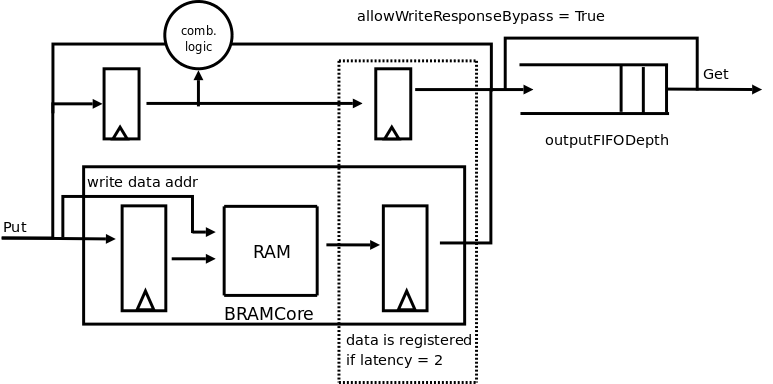
\includegraphics[width = 4 in]{LibFig/BRAM}
\caption{1 port of a BRAM Server}
\label{bram}
\end{center}
\end{figure}



\index{mkBRAM1Server@\te{mkBRAM1Server} (module)}
\index[function]{BRAM!mkBRAM1Server}
\label{sec-BRAM1Server}
\begin{tabular}{|p{1.4 in}|p{4.2 in}|}
\hline
& \\
\te{mkBRAM1Server}&BRAM Server module including an output FIFO and
logic to control  loading and to avoid overflow. \\
\cline{2-2}
& \begin{libverbatim}
module mkBRAM1Server #( BRAM_Configure cfg ) 
                      ( BRAM1Port #(addr, data) )
   provisos(Bits#(addr, addr_sz),
            Bits#(data, data_sz),
            DefaultValue#(data) );
\end{libverbatim}
\\
\hline
\end{tabular}
\label{sec-BRAM1ServerBE}
\index{mkBRAM1ServerBE@\te{mkBRAM1ServerBE} (module)}
\index[function]{BRAM!mkBRAM1ServerBE}

\begin{tabular}{|p{1.4 in}|p{4.2 in}|}
\hline
& \\
\te{mkBRAM1ServerBE}&Byte-enabled BRAM Server module. \\
\cline{2-2}
& \begin{libverbatim}
module mkBRAM1ServerBE #( BRAM_Configure cfg ) 
                        ( BRAM1PortBE #(addr, data, n) )
   provisos(Bits#(addr, addr_sz),
            Bits#(data, data_sz),
            Div#(data_sz, n, chunk_sz),
            Mul#(chunk_sz, n, data_sz), 
            DefaultValue#(data) );
\end{libverbatim}
\\
\hline
\end{tabular}


\index{mkBRAM2Server@\te{mkBRAM2Server} (module)}
\index[function]{BRAM!mkBRAM2Server}

\begin{tabular}{|p{1.4 in}|p{4.2 in}|}
\hline
& \\
\te{mkBRAM2Server}&2 port BRAM Server module. \\
\cline{2-2}
& \begin{libverbatim}
module mkBRAM2Server #( BRAM_Configure cfg ) 
                      ( BRAM2Port #(addr, data) )
   provisos(Bits#(addr, addr_sz),
            Bits#(data, data_sz),
            DefaultValue#(data) );
\end{libverbatim}
\\
\hline
\end{tabular}

\begin{tabular}{|p{1.4 in}|p{4.2 in}|}
\hline
& \\
\te{mkBRAM2ServerBE}&Byte-enabled 2 port BRAM Server module. \\
\cline{2-2}
& \begin{libverbatim}
module mkBRAM2ServerBE #( BRAM_Configure cfg ) 
                        ( BRAM2PortBE #(addr, data, n) )
   provisos(Bits#(addr, addr_sz),
            Bits#(data, data_sz),
            Div#(data_sz, n, chunk_sz),
            Mul#(chunk_sz, n, data_sz) );
\end{libverbatim}
\\
\hline
\end{tabular}



\index{mkSyncBRAM2Server@\te{mkSyncBRAM2Server} (module)}
\index[function]{BRAM!mkSyncBRAM2Server}

\begin{tabular}{|p{1.4 in}|p{4.2 in}|}
\hline
& \\
\te{mkSyncBRAM2Server}&2 port, dual clock,  BRAM Server module. The
\te{portA} subinterface and \te{portAClear} methods are in the
\te{clkA} domain;
the \te{portB} subinterface and \te{portBClear} methods are in the \te{clkB}
domain. \\
\cline{2-2}
& \begin{libverbatim}
(* no_default_clock, no_default_reset *)
module mkSyncBRAM2Server #( BRAM_Configure cfg,
                           Clock clkA, Reset rstNA,
                           Clock clkB, Reset rstNB
                           ) (BRAM2Port #(addr, data) )
   provisos(Bits#(addr, addr_sz),
            Bits#(data, data_sz),
            DefaultValue#(data) );

\end{libverbatim}
\\
\hline
\end{tabular}

\index{mkSyncBRAM2ServerBE@\te{mkSyncBRAM2ServerBE} (module)}
\index[function]{BRAM!mkSyncBRAM2ServerBE}

\begin{tabular}{|p{1.4 in}|p{4.2 in}|}
\hline
& \\
\te{mkSyncBRAM2ServerBE}&2 port, dual clock, byte-enabled BRAM Server
module. The 
\te{portA} subinterface and \te{portAClear} methods are in the
\te{clkA} domain;
the \te{portB} subinterface and \te{portBClear} methods are in the \te{clkB}
domain. \\
\cline{2-2}
& \begin{libverbatim}
(* no_default_clock, no_default_reset *)
module mkSyncBRAM2ServerBE #(BRAM_Configure cfg,
                             Clock clkA, Reset rstNA,
                             Clock clkB, Reset rstNB )
                          (BRAM2PortBE #(addr, data, n))
   provisos(Bits#(addr, addr_sz),
            Bits#(data, data_sz),
            Div#(data_sz, n, chunk_sz),
            Mul#(chunk_sz, n, data_sz) );
\end{libverbatim}
\\
\hline
\end{tabular}




{\bf Example: Using a BRAM}
\begin{verbatim}
import BRAM::*;
import StmtFSM::*;
import Clocks::*;

function BRAMRequest#(Bit#(8), Bit#(8)) makeRequest(Bool write, Bit#(8) addr, Bit#(8) data);
   return BRAMRequest{
                      write: write,
                      responseOnWrite:False,
                      address: addr,
                      datain: data
                      };
endfunction

(* synthesize *)
module sysBRAMTest();
    BRAM_Configure cfg = defaultValue;
    cfg.allowWriteResponseBypass = False;
    BRAM2Port#(Bit#(8), Bit#(8)) dut0 <- mkBRAM2Server(cfg);
    cfg.loadFormat = tagged Hex "bram2.txt";
    BRAM2Port#(Bit#(8), Bit#(8)) dut1 <- mkBRAM2Server(cfg);

   //Define StmtFSM to run tests
   Stmt test =
   (seq
       delay(10);
       ...
       action
          dut1.portA.request.put(makeRequest(False, 8'h02, 0));
          dut1.portB.request.put(makeRequest(False, 8'h03, 0));
       endaction
       action 
          $display("dut1read[0] = %x", dut1.portA.response.get);
          $display("dut1read[1] = %x", dut1.portB.response.get);
       endaction
       ...
       delay(100);
    endseq);
   mkAutoFSM(test);
endmodule
\end{verbatim}

\subsubsection{BRAMCore}
\index{BRAMCore (package}
%\index{Xilinx!BRAMCore (package)}
\label{sec-BRAMCore}


{\bf Package}

\begin{verbatim}
import BRAMCore :: * ;
\end{verbatim}



{\bf Description}

The \te{BRAMCore} package, along with the \te{BRAM} package (Section
\ref{sec-BRAM}) provides types, interfaces, and modules to support
FPGA BlockRAMS.  Specific tools may determine whether modules are
mapped to  appropriate BRAM cells during synthesis.

Most designs should use the  the \te{BRAM} package instead of
\te{BRAMCore}, as the \te{BRAM} package provides implicit conditions
provided by  FIFO wrappers.
The \te{BRAMCore} package should be used only if you want the
low-level core BRAM modules without  implicit conditions.

The \te{BRAMCore}  package contains the low-level wrappers to the BRAM
Verilog and Bluesim modules.  Components are provided for   single and
dual port,  byte-enabled,  loadable, and dual clock versions.



{\bf Interfaces and Methods}

\index{BRAM\_PORT@\te{BRAM\_PORT} (interface type)}
%\index{BRAM@\te{BRAM} (interface type)}
\index{BRAM\_DUAL\_PORT@\te{BRAM\_DUAL\_PORT} (interface type)}

The \te{BRAMCore} package defines four  variations of a BRAM 
interface to support  single
and dual port BRAMs, as well as byte-enabled BRAMs.

The \te{BRAM\_PORT} interface declares two methods; an Action method
\te{put}, and a value method \te{read}.

The \te{BRAM\_DUAL\_PORT} interface is defined as two \te{BRAM\_PORT}
subinterfaces, one for each port.

\begin{tabular}{|p{.4in}|p{.5 in}|p{1.2 in}|p{.5in}|p{2.5 in}|}
\hline
\multicolumn{5}{|c|}{BRAM\_PORT Interface}\\
\hline
\multicolumn{3}{|c|}{Method}&\multicolumn{2}{|c|}{Arguments}\\
\hline
Name & Type & Description& Name &\multicolumn{1}{|c|}{Description} \\
\hline
\hline 
\te{put}&\te{Action}&Read or write values in the 
BRAM.&\te{write}& Write enable for the port; if \te{True} the action
is write, if \te{False}, the action is  read.\\
\cline{4-5}
&&&\te{address}&Index of the element, with a datatype of \te{addr}. \\
\cline{4-5}
&&&\te{datain}& Value to be written, with a datatype of \te{data}. This value is ignored if the action is read.\\
\hline
\te{read}&\it{data}&Returns a value of  type \te{data}.  & &\\
\hline
\end{tabular}

\begin{verbatim}
(* always_ready *)
interface BRAM_PORT#(type addr, type data);
   method Action put(Bool write, addr address, data datain);
   method data   read();
endinterface: BRAM_PORT
\end{verbatim}

\begin{verbatim}
interface BRAM_DUAL_PORT#(type addr, type data);
   interface BRAM_PORT#(addr, data) a;
   interface BRAM_PORT#(addr, data) b;
endinterface
\end{verbatim}

{\bf Byte-enabled Interfaces}

The \te{BRAM\_PORT\_BE} and
\te{BRAM\_DUAL\_PORT\_BE} interfaces are the byte-enabled  versions of the
BRAM interfaces. 
In this version, the  argument \te{writen} is of type
\te{Bit\#(n)}, where  \te{n} is  the number of byte-enables.  Your
synthesis tools and targeted technology determine the restriction of
data size and byte enable size.  If $n = 0$, the action is a read.  

The \te{BRAM\_DUAL\_PORT\_BE} interface is defined as two \te{BRAM\_PORT\_BE}
subinterfaces, one for each port.


\begin{tabular}{|p{.4in}|p{.5 in}|p{1.2 in}|p{.5in}|p{2.5 in}|}
\hline
\multicolumn{5}{|c|}{BRAM\_PORT\_BE Interface}\\
\hline
\multicolumn{3}{|c|}{Method}&\multicolumn{2}{|c|}{Arguments}\\
\hline
Name & Type & Description& Name &\multicolumn{1}{|c|}{Description} \\
\hline
\hline 
\te{put}&\te{Action}&Read or write  values in the
BRAM.  &\te{writeen}& Byte-enable for the port; if \te{n} != 0 write the
specified bytes,  if \te{n} = 0 read.  \\
\cline{4-5}
&&&\te{address}&Index of the elements to be read or written, with a datatype of \te{addr}. \\
\cline{4-5}
&&&\te{datain}& Value to be written, with a datatype of \te{data}.
This value is ignored if the action is read.\\
\hline
\te{read}&\it{data}&Returns a value of  type \te{data}.&&\\
\hline
\end{tabular}



\begin{verbatim}
(* always_ready *)
interface BRAM_PORT_BE#(type addr, type data, numeric type n);
   method Action put(Bit#(n) writeen, addr address, data datain);
   method data   read();
endinterface: BRAM_PORT_BE
\end{verbatim}

\begin{verbatim}
interface BRAM_DUAL_PORT_BE#(type addr, type data, numeric type n);
   interface BRAM_PORT_BE#(addr, data, n) a;
   interface BRAM_PORT_BE#(addr, data, n) b;
endinterface
\end{verbatim}


{\bf Modules}

The \te{BRAMCore} package provides 1 and 2 port BRAM core modules, in both
write-enabled and byte-enabled versions.  Note that there are no
implicit conditions on the methods of these modules; if these are
required consider using the modules in the \te{BRAM} package (Section
\ref{sec-BRAM}).  


The \te{BRAMCore} package requires the caller to
 ensure the correct cycle to capture the read data, as
 determined by  the \te{hasOutputRegister} flag.  If \te{hasOutputRegister} 
is \te{True}, both the read address and the read data are registered;
if \te{False}, only the read address is registered.

\begin{itemize}
\item If the output is registered (\te{hasOutputRegister} is \te{True}), the latency is 2; the read data is
available 2 cycles after the request. 
\item If the output is not registered (\te{hasOutputRegister} is \te{False}), the latency is 1; the read data
is available 1 cycle after the request.
\end{itemize}

The other argument  required is  \te{memSize},  an \te{Integer} 
specifying the memory size in number of words of type \te{data}.  


 The loadable BRAM modules require two additional arguments:
\begin{itemize}
\item \te{file} is a \te{String} containing the name of the load file.
\item \te{binary} is a \te{Bool} indicating whether 
 the data type of the load file is binary (\te{True}) or
hex (\te{False}).
\end{itemize}


\index{mkBRAMCore1@\te{mkBRAMCore1} (module)}
\index[function]{BRAM!mkBRAMCore1}

\begin{tabular}{|p{1.4 in}|p{4.2 in}|}
\hline
& \\
\te{mkBRAMCore1} &Single port BRAM \\
\cline{2-2}
& \begin{libverbatim}
module mkBRAMCore1#(Integer memSize,
               Bool hasOutputRegister) 
               (BRAM_PORT#(addr, data))
   provisos(Bits#(addr, addr_sz), Bits#(data, data_sz));
\end{libverbatim}
\\
\hline
\end{tabular}


\index{mkBRAMCore1BE@\te{mkBRAMCore1BE} (module)}
\index[function]{BRAM!mkBRAMCore1BE}

\begin{tabular}{|p{1.4 in}|p{4.2 in}|}
\hline
& \\
\te{mkBRAMCore1BE} &Byte-enabled, single port BRAM. \\
\cline{2-2}
& \begin{libverbatim}
module mkBRAMCore1BE#(Integer memSize,
                  Bool hasOutputRegister ) 
                 (BRAM_PORT_BE#(addr, data, n))
   provisos(Bits#(addr, addr_sz), Bits#(data, data_sz),
            Div#(data_sz, n, chunk_sz), 
            Mul#(chunk_sz, n, data_sz));
\end{libverbatim}
\\
\hline
\end{tabular}

% The \te{file} provides the initial contents of the BRAM.  If
% \te{binary} is \te{True} it is a binary file, if \te{False} it is a
% hex file.

\index{mkBRAMCore1Load@\te{mkBRAMCore1Load} (module)}
\index[function]{BRAM!mkBRAMCore1Load}

\begin{tabular}{|p{1.4 in}|p{4.2 in}|}
\hline
& \\
\te{mkBRAMCore1Load} &Loadable, single port BRAM where the initial
contents are in \te{file}.  The parameter \te{binary} indicates whether the
contents of \te{file} are  binary (\te{True}) or hex (\te{False}). \\
\cline{2-2}
& \begin{libverbatim}
module mkBRAMCore1Load#(Integer memSize, 
                        Bool hasOutputRegister,
                        String file, Bool binary )
                       (BRAM_PORT#(addr, data))
   provisos(Bits#(addr, addr_sz), Bits#(data, data_sz) );
\end{libverbatim}
\\
\hline
\end{tabular}

\index{mkBRAMCore1BELoad@\te{mkBRAMCore1BELoad} (module)}
\index[function]{BRAM!mkBRAMCore1BELoad}

\begin{tabular}{|p{1.4 in}|p{4.2 in}|}
\hline
& \\
\te{mkBRAMCore1BELoad} &Loadable, single port, byte-enabled BRAM. \\
\cline{2-2}
& \begin{libverbatim}
module mkBRAMCore1BELoad#(Integer memSize,
                          Bool hasOutputRegister,
                          String file, Bool binary) 
                         (BRAM_PORT_BE#(addr, data, n))
   provisos(Bits#(addr, addr_sz), Bits#(data, data_sz),
            Div#(data_sz, n, chunk_sz),
            Mul#(chunk_sz, n, data_sz) );
\end{libverbatim}
\\
\hline
\end{tabular}



\index{mkBRAMCore2@\te{mkBRAMCore2} (module)}
\index[function]{BRAM!mkBRAMCore2}

\begin{tabular}{|p{1.4 in}|p{4.2 in}|}
\hline
& \\
\te{mkBRAMCore2} &Dual port, single clock BRAM. \\
\cline{2-2}
& \begin{libverbatim}
module mkBRAMCore2#(Integer memSize,
                    Bool hasOutputRegister ) 
                   (BRAM_DUAL_PORT#(addr, data))
   provisos(Bits#(addr, addr_sz), Bits#(data, data_sz) );
\end{libverbatim}
\\
\hline
\end{tabular}


\index{mkBRAMCore2BE@\te{mkBRAMCore2BE} (module)}
\index[function]{BRAM!mkBRAMCore2BE}

\begin{tabular}{|p{1.4 in}|p{4.2 in}|}
\hline
& \\
\te{mkBRAMCore2BE} &Byte-enabled, dual port BRAM. \\
\cline{2-2}
& \begin{libverbatim}
module mkBRAMCore2BE#(Integer memSize,
                      Bool hasOutputRegister
                     ) (BRAM_DUAL_PORT_BE#(addr, data, n))
   provisos(Bits#(addr, addr_sz),
            Bits#(data, data_sz),
            Div#(data_sz, n, chunk_sz),
            Mul#(chunk_sz, n, data_sz) );
\end{libverbatim}
\\
\hline
\end{tabular}


\index{mkSyncBRAMCore2@\te{mkSyncBRAMCore2} (module)}
\index[function]{BRAM!mkSyncBRAMCore2}

\begin{tabular}{|p{1.4 in}|p{4.2 in}|}
\hline
& \\
\te{mkSyncBRAMCore2} &Dual port, dual clock BRAM. \\
\cline{2-2}
& \begin{libverbatim}
module mkSyncBRAMCore2#(Integer memSize,
                    Bool hasOutputRegister,
                    Clock clkA, Reset rstNA,
                    Clock clkB, Reset rstNB )
                    (BRAM_DUAL_PORT#(addr, data))
   provisos(Bits#(addr, addr_sz),Bits#(data, data_sz));
\end{libverbatim}
\\
\hline
\end{tabular}

\index{mkSyncBRAMCore2BE@\te{mkSyncBRAMCore2BE} (module)}
\index[function]{BRAM!mkSyncBRAMCore2BE}

\begin{tabular}{|p{1.4 in}|p{4.2 in}|}
\hline
& \\
\te{mkSyncBRAMCore2BE} &Dual port, dual clock byte-enabled BRAM. \\
\cline{2-2}
& \begin{libverbatim}
module mkSyncBRAMCore2BE#(Integer memSize,
                          Bool hasOutputRegister,
                          Clock clkA, Reset rstNA,
                          Clock clkB, Reset rstNB)
                       (BRAM_DUAL_PORT_BE#(addr, data, n))
   provisos(Bits#(addr, addr_sz),
            Bits#(data, data_sz),
            Div#(data_sz, n, chunk_sz),
            Mul#(chunk_sz, n, data_sz) );
\end{libverbatim}
\\
\hline
\end{tabular}

\index{mkBRAMCore2Load@\te{mkBRAMCore2Load} (module)}
\index[function]{BRAM!mkBRAMCore2Load}

\begin{tabular}{|p{1.4 in}|p{4.2 in}|}
\hline
& \\
\te{mkBRAMCore2Load} &Dual port, single clock,  BRAM where the initial contents are
in \te{file}.  The parameter \te{binary} indicates whether the
contents of \te{file} are  binary (\te{True}) or hex (\te{False}).  \\
\cline{2-2}
& \begin{libverbatim}
module mkBRAMCore2Load#(Integer memSize,
                        Bool hasOutputRegister,
                        String file, Bool binary)
                       (BRAM_DUAL_PORT#(addr, data))
   provisos(Bits#(addr, addr_sz),Bits#(data, data_sz));
\end{libverbatim}
\\
\hline
\end{tabular}


\index{mkBRAMCore2BELoad@\te{mkBRAMCore2BELoad} (module)}
\index[function]{BRAM!mkBRAMCore2BELoad}

\begin{tabular}{|p{1.4 in}|p{4.2 in}|}
\hline
& \\
\te{mkBRAMCore2BELoad} &Dual port, single clock, byte-enabled  BRAM where the initial contents are
in \te{file}.  The parameter \te{binary} indicates whether the
contents of \te{file} are  binary (\te{True}) or hex (\te{False}).  \\
\cline{2-2}
& \begin{libverbatim}
module mkBRAMCore2BELoad#(Integer memSize,
                          Bool hasOutputRegister,
                          String file, Bool binary )
                    (BRAM_DUAL_PORT_BE#(addr, data, n))
   provisos(Bits#(addr, addr_sz),
            Bits#(data, data_sz),
            Div#(data_sz, n, chunk_sz),
            Mul#(chunk_sz, n, data_sz) );
\end{libverbatim}
\\
\hline
\end{tabular}

\index{mkSyncBRAMCore2Load@\te{mkSyncBRAMCore2Load} (module)}
\index[function]{BRAM!mkSyncBRAMCore2Load}

\begin{tabular}{|p{1.4 in}|p{4.2 in}|}
\hline
& \\
\te{mkSyncBRAMCore2Load} & Dual port, dual clock BRAM with initial
contents in \te{file}.\\
\cline{2-2}
& \begin{libverbatim}
module mkSyncBRAMCore2Load#(Integer memSize,
                        Bool hasOutputRegister,
                        Clock clkA, Reset rstNA,
                        Clock clkB, Reset rstNB,
                        String file, Bool binary)
                        (BRAM_DUAL_PORT#(addr, data))
   provisos(Bits#(addr, addr_sz), Bits#(data, data_sz));
\end{libverbatim}
\\
\hline
\end{tabular}

\index{mkSyncBRAMCore2BELoad@\te{mkSyncBRAMCore2BELoad} (module)}
\index[function]{BRAM!mkSyncBRAMCore2BELoad}

\begin{tabular}{|p{1.4 in}|p{4.2 in}|}
\hline
& \\
\te{mkSyncBRAMCore2BELoad} & Dual port, dual clock, byte-enabledBRAM
with initial contents in \te{file}.\\
\cline{2-2}
& \begin{libverbatim}
module mkSyncBRAMCore2BELoad#(Integer memSize,
                              Bool hasOutputRegister,
                              Clock clkA, Reset rstNA,
                              Clock clkB, Reset rstNB,
                              String file, Bool binary)
                       (BRAM_DUAL_PORT_BE#(addr, data, n))
   provisos(Bits#(addr, addr_sz),
            Bits#(data, data_sz),
            Div#(data_sz, n, chunk_sz),
            Mul#(chunk_sz, n, data_sz) );
\end{libverbatim}
\\
\hline
\end{tabular}





{\bf Verilog Modules}

\te{BRAM} modules correspond to the following {\V}
modules, which are found in the Bluespec {\V} library, \te{\$BLUESPECDIR/Verilog/}.

\begin{center}
\begin{tabular} {|p{2.5 in}|p{2.5 in}|}
\hline
&\\
BSV Module Name & Verilog Module Names \\
&\\
\hline
\hline
\te{mkBRAMCore1}&\te{BRAM1.v}  \\
\hline
\te{mkBRAMCore1Load}&\te{BRAM1Load.v}\\
\hline
\te{mkBRAMCore1BE}&\te{BRAM1BE.v} \\
\hline
\te{mkBRAMCore1BELoad}&\te{BRAM1BELoad.v}  \\
\hline
\te{mkBRAMCore2}&\te{BRAM2.v}  \\
\te{mkSyncBRAMCore2}& \\
\hline
\te{mkBRAMCore2BE}&\te{BRAM2BE.v}\\
\te{mkSyncBRAMCore2BE}&\\
\hline
\te{mkBRAMCore2Load}&\te{BRAM2Load.v}  \\
\te{mkSyncBRAMCore2Load}& \\
\hline
\te{mkBRAMCore2BELoad}&\te{BRAM2BELoad.v}\\
\te{mkSyncBRAMCore2BELoad}&\\
\hline

\end{tabular}
\end{center}


% ----------------

\subsection{FIFOs}

\subsubsection{FIFO Overview}
 

The BSC library contains multiple FIFO packages.


\begin{center}
\begin{tabular}{|l|p{3.5in}|c|l|}
\hline
&&&\\
Package Name&Description&BSV Source&Section\\
&&provided&\\
\hline
FIFO&Defines the FIFO interface and module constructors.   FIFOs provided have
 implicit full and empty signals.  Includes pipeline FIFO (\te{mkLFIFO}).& &\ref{sec-FIFO}\\
\hline
FIFOF&Defines the FIFOF interface and module constructors.   FIFOs
provided have explicit full and empty signals.  Includes pipeline
FIFOF (\te{mkLFIFOF}).&&\ref{sec-FIFO}\\
\hline
FIFOLevel&Enhanced FIFO interfaces and modules which include methods
to indicate the level or current number of items stored in the FIFO.
Single and dual clock versions are provided.&&\ref{FIFOLevel}\\
\hline
BRAMFIFO&FIFOs which utilize the Xilinx Block RAMs.&$\surd$&\ref{sec-BRAMFIFO}\\
\hline
SpecialFIFOs&Additional pipeline and bypass FIFOs&$\surd$&\ref{sec-SpecialFIFOs}\\
\hline
AlignedFIFOs&Parameterized FIFO module for creating synchronizing
FIFOs between clock domains with aligned edges.&$\surd$&\ref{sec-AlignedFIFOs}\\
\hline
Gearbox&FIFOs which change the frequency and data width of data
across clock domains with aligned edges.  The overall data rate stays the samme.&$\surd$&\ref{Gearbox}\\
\hline
Clocks&Generalized FIFOs to synchronize data being sent across clock
domains&&\ref{syncfifoifc}\\
\hline
\end{tabular}
\end{center}



% There are three FIFO packages, \te{FIFO}, \te{FIFOF}, and
% \te{FIFOLevel}. The following table shows when to use each FIFO,
% and which methods are in implemented in each FIFO.  All FIFOs
% include the methods \te{enq}, \te{deq}, \te{first}, \te{clear}.
% These are referred to as the common methods in the table.

% \begin{center}
% \begin{tabular} {|l|l|l|}
% \hline
% & &  \\
% Package Name & Description &  Methods \\
% \hline 
% \hline
% All FIFO  & common methods in all FIFOs  &\te{enq} \\
% packages & &  \te{deq}\\
% & &  \te{first}\\
% & &  \te{clear} \\
% \hline
% FIFO & Implicit full and empty signals & common methods\\
% \hline
% FIFOF & Explicit full and empty signals &  common methods\\
% & &  \te{notFull} \\
% & &  \te{notEmpty} \\
% \hline
% FIFOLevel & Indicates the level or current number & 
% common methods\\
% & of items stored in the FIFO &  \te{notFull}\\
% & &  \te{notEmpty} \\
% & &  \te{isLessThan} \\
% & &  \te{isGreaterThan} \\
% %& &  \te{maxDepth} \\
% \hline
% \end{tabular}
% \end{center}

% {\bf Common Methods}

% The following four methods are provided in all  FIFO packages.

% \begin{center}
% \begin{tabular}{|p{.5in}|p{.7in}|p{1.5 in}|p{.4in}|p{1.9 in}|}
% \hline
% \multicolumn{3}{|c|}{Method}&\multicolumn{2}{|c|}{Argument}\\
% \hline
% Name & Type & Description& Name &\multicolumn{1}{|c|}{Description} \\
% \hline
% \hline 
% \te{enq}  & Action & adds an entry to the \te{FIFO}& x1 & variable
% to be added to the \te{FIFO}\\
% & & & & must be of type \it{element\_type} \\
% \hline
% \te{deq} & Action & removes first entry from the \te{FIFO}  & &  \\
% \hline
% \te{first}  & \it{element\_type} & returns first entry  & & the
% entry returned is of \\ 
% & & & &\it{element\_type} \\
% \hline
% \te{clear}  & Action & clears all entries from the \te{FIFO} & &\\
% \hline
% \end{tabular}
% \end{center}

\subsubsection{FIFO and FIFOF packages}

\label{sec-FIFO}

{\bf Packages}
\index{FIFO@\te{FIFO} (package)}
\index{FIFOF@\te{FIFOF} (package)}


\begin{verbatim}
import FIFO :: * ;
import FIFOF :: * ;
\end{verbatim}


{\bf Description}

The FIFO package defines the  \te{FIFO} interface and four module
constructors.  The \te{FIFO} package is for FIFOs with implicit
full and empty signals.  

The  \te{FIFOF} package defines FIFOs with explicit full and empty signals. 
The standard version of \te{FIFOF} has FIFOs with the enq, 
deq and first methods guarded by the appropriate (notFull or notEmpty)
implicit conditions for safety and improved scheduling. 
Unguarded (UG) versions of \te{FIFOF} are available for the rare cases
when implicit conditions are not desired. 
Guarded (G) versions of \te{FIFOF} are
available which allow more control over implicit conditions.  With the
guarded versions the user can specify whether the enqueue or dequeue
side is guarded.

{\bf Type classes}


\paragraph{FShow}

The \te{FIFOF} type belongs to the \te{FShow} type class.  A
\te{FIFOF} can be turned into a \te{Fmt} type.  The \te{Fmt} value
returned depends on the values of the \te{notEmpty} and \te{notFull} 
methods.

\begin{tabular}{|p{1in}|p{1in}|p{1in}|p{1in}|}
\hline
\multicolumn{4}{|c|}{FShow values for FIFOF}\\
\hline
\hline
notEmpty & notFull& Fmt Object & Example\\
\hline
True&True&\te{<first>}&3\\
True&False&\te{<first> FULL}&2 FULL\\
False&True & \te{EMPTY}& \te{EMPTY}\\
False&False & \te{EMPTY} & \te{EMPTY}\\
\hline
\multicolumn{4}{|l|}{\te{Note: <first>} is the  value of the first
entry with the  fshow function applied }\\
\hline
\end{tabular}


{\bf Interfaces and methods} 
\label{sec-FIFOifc}

% \begin{tabular}{|l|l|l|l|}
%  \hline
%                           &                                     &
% &               \\
% Interface Name   & Parameter name & Parameter Description & Restrictions \\
% \hline
% \hline
% \te{FIFO} & \it{element\_type} & type of the elements &must be in
% \te{Bits} class \\
% & &stored in the \te{FIFO} &\\
% \hline
% \te{FIFOF} & \it{element\_type} & type of the elements &must be in
% \te{Bits} class \\
% & &stored in the \te{FIFO} &\\
% \hline
% \end{tabular}

The four common methods, \te{enq}, \te{deq}, \te{first} and \te{clear}
are provided by both the \te{FIFO} and \te{FIFOF} interfaces.

\begin{center}
\begin{tabular}{|p{.5in}|p{.7in}|p{1.5 in}|p{.4in}|p{1.9 in}|}
\hline
\multicolumn{5}{|c|}{FIFO methods}\\
\hline
\multicolumn{3}{|c|}{Method}&\multicolumn{2}{|c|}{Argument}\\
\hline
Name & Type & Description& Name &\multicolumn{1}{|c|}{Description} \\
\hline
\hline 
\te{enq}  & Action & adds an entry to the \te{FIFO}& x1 & variable
to be added to the \te{FIFO}\\
& & & & must be of type \it{element\_type} \\
\hline
\te{deq} & Action & removes first entry from the \te{FIFO}  & &  \\
\hline
\te{first}  & \it{element\_type} & returns first entry  & & the
entry returned is of \it{element\_type} \\
\hline
\te{clear}  & Action & clears all entries from the \te{FIFO} & &\\
\hline
\end{tabular}
\end{center}
\begin{libverbatim}
interface FIFO #(type element_type);
    method Action enq(element_type x1);
    method Action deq();
    method element_type first();
    method Action clear();
endinterface: FIFO
\end{libverbatim}

\te{FIFOF} provides two additional methods, \te{notFull} and
\te{notEmpty}.
 
\begin{center}
\begin{tabular}{|p{.75in}|p{.75in}|p{3.5 in}|}
\hline
\multicolumn{3}{|c|}{Additional FIFOF Methods}\\
\hline
Name & Type & Description\\
\hline
\te{notFull} & Bool & returns a True value if there is space, you can
enqueue an entry into the FIFO  \\
\hline
\te{notEmpty} & Bool &returns a True value if there are elements the
FIFO, you can dequeue from the FIFO   \\
\hline
\end{tabular}
\end{center}

\begin{verbatim}
interface FIFOF #(type element_type);
    method Action enq(element_type x1);
    method Action deq();
    method element_type first();
    method Bool notFull();
    method Bool notEmpty();
    method Action clear();
endinterface: FIFOF
\end{verbatim}

The \te{FIFO} and \te{FIFOF} interfaces belong to the \te{ToGet} and
\te{ToPut} typeclasses.  You can use the \te{toGet} and \te{toPut}
functions to convert \te{FIFO} and \te{FIFOF} interfaces to \te{Get}
and \te{Put} interfaces (Section \ref{sec-GetPut}). 




{\bf Modules}
\index{mkFIFO@\te{mkFIFO} (module)}
\label{sec-fifo-mod}

The \te{FIFO} and \te{FIFOF} interface types are provided by the
module  constructors: \te{mkFIFO}, \te{mkFIFO1}, \te{mkSizedFIFO},
\te{mkDepthParamFIFO}, and \te{mkLFIFO}.
Each \te{FIFO} is safe with implicit conditions; they do not allow
an \te{enq} when the \te{FIFO} is full or  a
\te{deq} or  \te{first}
when the \te{FIFO} is empty.  

Most FIFOs  do not allow  simultaneous enqueue and
dequeue operations when the FIFO is full or empty.  The exceptions are pipeline
 and bypass FIFOs.  A  pipeline FIFO (provided as \te{mkLFIFO} in this
 package),  allows 
simultaneous enqueue and dequeue operations when full.  A bypass FIFO
allows simultaneous enqueue and  dequeue operations  when empty. Additional pipeline and bypass FIFOs are provided in the \te{SpecialFIFOs} package (Section
 \ref{sec-SpecialFIFOs}).    The FIFOs in the \te{SpecialFIFOs}
 package are provided as both compiled code and BSV source code,
so they are customizable.

\begin{center}
\begin{tabular}{|p{2 in}|c|c|c|}
\hline
\multicolumn{4}{|c|}{Allowed Simultaneous enq and deq }\\
\multicolumn{4}{|c|}{by FIFO type}\\
%\multicolumn{4}{|c|}{}\\
\hline
&\multicolumn{3}{|c|}{FIFO Condition}\\
\cline{2-4}
FIFO type&empty&not empty&full\\
&&not full &\\
\hline
\hline
\te{mkFIFO}&&$\surd$&\\
\te{mkFIFOF}&&&\\
\hline
\te{mkFIFO1}&&NA&\\
\te{mkFIFOF1}&&&\\
\hline
\te{mkLFIFO}&&$\surd$&$\surd$\\
\te{mkLFIFOF}&&&\\
\hline
\te{mkLFIFO1}&&NA&$\surd$\\
\te{mkLFIFOF1}&&&\\
\hline
\multicolumn{4}{|c|}{Modules provided in SpecialFIFOs package \ref{sec-SpecialFIFOs}} \\
\hline
\te{mkPipelineFIFO}&&NA&$\surd$\\
\te{mkPipelineFIFOF}&&&\\
\hline
\te{mkBypassFIFO}&$\surd$&NA&\\
\te{mkBypassFIFOF}&&&\\
\hline
\te{mkSizedBypassFIFOF}&$\surd$&$\surd$&\\
\hline
\te{mkBypassFIFOLevel}&$\surd$&$\surd$&\\
\hline
\hline
\end{tabular}
\end{center}

For creating a \te{FIFOF}  interface (providing explicit \te{notFull} and
\te{notEmpty} methods) use the \te{"F"} version of the
module, for example use \te{mkFIFOF} instead of \te{mkFIFO}.




\index[function]{FIFOF!mkFIFOF}
\index[function]{FIFO!mkFIFO}
\index{mkFIFOF@\te{mkFIFOF} (module)}



\begin{center}
\begin{tabular}{|p{1.1 in}|p{4.4 in}|}
 \hline
  &            \\
Module Name  &  BSV Module Declaration   \\
&\emph{For all modules, \te{width\_any} may be 0}  \\
\hline
\multicolumn{2}{|l|}{\te{FIFO} or \te{FIFOF} of depth 2.}\\
\hline
\begin{libverbatim}mkFIFO 
mkFIFOF 
\end{libverbatim} 
& \begin{libverbatim}module mkFIFO#(FIFO#(element_type)) 
   provisos (Bits#(element_type, width_any));
 \end{libverbatim} 
\\
\hline
\end{tabular}
\end{center}




\index[function]{FIFO!mkFIFO1}
\index[function]{FIFOF!mkFIFOF1}

\index{mkFIFOF1@\te{mkFIFOF1} (module)}
\index{mkFIFO1@\te{mkFIFO1} (module)}


\begin{center}
\begin{tabular}{|p{1.1 in}|p{4.4 in}|}
\hline
\multicolumn{2}{|l|}{\te{FIFO} or \te{FIFOF} of depth 1}\\
\hline
\begin{libverbatim}mkFIFO1
mkFIFOF1
\end{libverbatim}
& \begin{libverbatim}
module mkFIFO1#(FIFO#(element_type))
   provisos (Bits#(element_type, width_any)); \end{libverbatim} 
\\
\hline
\end{tabular}
\end{center}





\index[function]{FIFO!mkSizedFIFO}
\index[function]{FIFOF!mkSizedFIFOF}
\index{mkSizedFIFOF@\te{mkSizedFIFOF} (module)}
\index{mkSizedFIFO@\te{mkSizedFIFO} (module)}

\begin{center}
\begin{tabular}{|p{1.1 in}|p{4.4 in}|}
\hline
\multicolumn{2}{|l|}{\te{FIFO} or \te{FIFOF} of given depth n}\\
\hline
\begin{libverbatim}mkSizedFIFO
mkSizedFIFOF
\end{libverbatim}
& \begin{libverbatim}
module mkSizedFIFO#(Integer n)(FIFO#(element_type))  
   provisos (Bits#(element_type, width_any)); \end{libverbatim}
 \\
\hline 
\end{tabular}
\end{center}


% The \te{FIFOF} package also provides sized FIFOs where the depth
% \te{n} is of type \te{UInt\#(32)} and is a Verilog parameter or
% computed from compile-time constants and Verilog parameters.  Buarded
% and unguarded versions of the depth parameter FIFOs are provided.

\index[function]{FIFO!mkDepthParamFIFO}
\index[function]{FIFOF!mkDepthParamFIFOF}
\index{mkDepthParamFIFOF@\te{mkDepthParamFIFOF} (module)}
\index{mkDepthParamFIFO@\te{mkDepthParamFIFO} (module)}

\begin{center}
\begin{tabular}{|p{1.3 in}|p{4.2 in}|}
\hline
\multicolumn{2}{|l|}{\te{FIFO} or \te{FIFOF} of given depth n where n
is a Verilog parameter or computed from }\\
\multicolumn{2}{|l|}{compile-time constants and Verilog
parameters.}\\
\hline
\begin{libverbatim}mkDepthParamFIFO
mkDepthParamFIFOF
\end{libverbatim}
& \begin{libverbatim}
module mkDepthParamFIFO#(UInt#(32) n)(FIFO#(element_type))  
  provisos (Bits#(element_type, width_any)); \end{libverbatim}
 \\  
&    \\
\hline 
\end{tabular}
\end{center}





Unguarded (UG) versions of \te{FIFOF} are available for the rare cases
when implicit conditions are not desired.  When using an unguarded
FIFO, the implicit conditions for correct FIFO 
operations are NOT considered  during rule and method processing,
making it 
possible to enqueue when full and to dequeue when empty. 
These modules  provide the \te{FIFOF}
interface. 


\index[function]{FIFOF!mkUGFIFOF}
\index{mkUGFIFOF@\te{mkUGFIFOF} (module)}


\begin{center}
\begin{tabular}{|p{1.1 in}|p{4.4 in}|}
 \hline
\multicolumn{2}{|l|}{Unguarded FIFOF of depth 2}\\
\hline
\te{mkUGFIFOF}
& \begin{libverbatim}module mkUGFIFOF#(FIFOF#(element_type)) 
   provisos (Bits#(element_type, width_any));
 \end{libverbatim} 
\\
\hline
\end{tabular}
\end{center}


\index[function]{FIFOF!mkUGFIFO1}
\index{mkUGFIFOF1@\te{mkUGFIFOF1} (module)}


\begin{center}
\begin{tabular}{|p{1.1 in}|p{4.4 in}|}
\hline
\multicolumn{2}{|l|}{Unguarded \te{FIFOF} of depth 1}\\
\hline
\te{mkUGFIFOF1}
& \begin{libverbatim}
module mkUGFIFO1#(FIFOF#(element_type))
   provisos (Bits#(element_type, width_any)); \end{libverbatim} 
\\
\hline
\end{tabular}
\end{center}


\index[function]{FIFOF!mkUGSizedFIFOF}
\index{mkUGSizedFIFOF@\te{mkUGSizedFIFOF} (module)}
\begin{center}
\begin{tabular}{|p{1.1 in}|p{4.4 in}|}
\hline
\multicolumn{2}{|l|}{Unguarded \te{FIFOF} of given depth n}\\
\hline
\te{mkUGSizedFIFOF}
& \begin{libverbatim}
module mkUGSizedFIFOF#(Integer n)(FIFOF#(element_type))  
   provisos (Bits#(element_type, width_any)); \end{libverbatim}
 \\
\hline 
\end{tabular}
\end{center}

\index[function]{FIFOF!mkUGDepthParamFIFOF}
\index{mkUGDepthParamFIFOF@\te{mkUGDepthParamFIFOF} (module)}

\begin{center}
\begin{tabular}{|p{1.3 in}|p{4.2 in}|}
\hline
\multicolumn{2}{|l|}{Unguarded \te{FIFO} of given depth n where n is a Verilog
parameter or computed from }\\
\multicolumn{2}{|l|}{compile-time constants and Verilog
parameters.}\\
\hline
\te{mkUGDepthParamFIFOF}
& \begin{libverbatim}
module mkUGDepthParamFIFOF#(UInt#(32) n)
                          (FIFOF#(element_type))  
  provisos (Bits#(element_type, width_any)); \end{libverbatim}
 \\  
&    \\
\hline 
\end{tabular}
\end{center}



The  guarded (G) versions of each of the
\te{FIFOF}s allow you to specify which implicit condition you want
to guard.  These modules takes two  Boolean
parameters; \te{ugenq} and \te{ugdeq}.  Setting either parameter
\te{TRUE} indicates the relevant methods (\te{enq} for \te{ugenq},
\te{first} and \te{deq} for
\te{ugdeq}) are unguarded.  If both are \te{TRUE} the
\te{FIFOF} behaves the same as an unguarded \te{FIFOF}.  If both are
\te{FALSE} the behavior is the same as a regular \te{FIFOF}.  



\index[function]{FIFOF!mkGFIFOF}
\index{mkGFIFOF@\te{mkGFIFOF} (module)}


\begin{center}
\begin{tabular}{|p{1.1 in}|p{4.6 in}|}
 \hline
\multicolumn{2}{|l|}{Guarded \te{FIFOF} of depth 2.}\\
\hline
\begin{libverbatim}mkGFIFOF 
\end{libverbatim} 
& \begin{libverbatim}
module mkGFIFOF#(Bool ugenq, Bool ugdeq)(FIFOF#(element_type)) 
   provisos (Bits#(element_type, width_any));
 \end{libverbatim} 
\\
\hline
\end{tabular}
\end{center}




\index[function]{FIFOF!mkGFIFOF1}
\index{mkGFIFOF1@\te{mkGFIFOF1} (module)}


\begin{center}
\begin{tabular}{|p{1.1 in}|p{4.6 in}|}
\hline
\multicolumn{2}{|l|}{Guarded \te{FIFOF} of depth 1}  \\
\hline
\begin{libverbatim}mkGFIFOF1
\end{libverbatim}
& \begin{libverbatim}
module mkGFIFOF1#(Bool ugenq, Bool ugdeq)(FIFOF#(element_type))
   provisos (Bits#(element_type, width_any)); \end{libverbatim} 
\\
\hline
\end{tabular}
\end{center}




\index[function]{FIFOF!mkGSizedFIFOF}
\index{mkGSizedFIFOF@\te{mkGSizedFIFOF} (module)}
\begin{center}
\begin{tabular}{|p{1.1 in}|p{4.6 in}|}
\hline
\multicolumn{2}{|l|}{Guarded \te{FIFOF} of given depth n }\\
\hline
\begin{libverbatim}mkGSizedFIFOF
\end{libverbatim}
& \begin{libverbatim}
module mkGSizedFIFOF#(Bool ugenq, Bool ugdeq, Integer n)
                    (FIFOF#(element_type))  
  provisos (Bits#(element_type, width_any)); \end{libverbatim}
  \\
   &  \\
\hline 
\end{tabular}
\end{center}


\index[function]{FIFOF!mkGDepthParamFIFOF}
\index{mkGDepthParamFIFOF@\te{mkGDepthParamFIFOF} (module)}

\begin{center}
\begin{tabular}{|p{1.3 in}|p{4.4 in}|}
\hline
\multicolumn{2}{|l|}{Guarded \te{FIFOF} of given depth n where n is a Verilog
parameter or computed from }\\
\multicolumn{2}{|l|}{compile-time constants and Verilog
parameters.}\\
\hline
\begin{libverbatim}mkGDepthParamFIFOF
\end{libverbatim}
& \begin{libverbatim}
module mkGDepthParamFIFOF#(Bool ugenq, Bool ugdeq, UInt#(32) n)
           (FIFOF#(element_type))  
  provisos (Bits#(element_type, width_any)); \end{libverbatim}
  \\
   &  \\
\hline 
\end{tabular}
\end{center}


The \te{LFIFO}s (pipeline FIFOs)  allow \te{enq} and \te{deq} in the same clock cycle
when the FIFO is full.  Additional BSV versions of the pipeline FIFO and also
bypass FIFOs (allowing simultaneous \te{enq} and \te{deq} when the
FIFO is empty) are provided in the \te{SpecialFIFOs} package (Section
\ref{sec-SpecialFIFOs}).  Both unguarded and guarded versions of the
\te{LFIFO} are provided in the \te{FIFOF} package.


\index[function]{FIFO!mkLFIFO}
\index[function]{FIFOF!mkLFIFOF}
\index[function]{FIFOF!mkUGLFIFOF}
\index{mkLFIFOF@\te{mkLFIFOF} (module)}
\index{mkUGLFIFOF@\te{mkUGLFIFOF} (module)}
\index{mkLFIFO@\te{mkLFIFO} (module)}
\begin{center}
\begin{tabular}{|p{.9 in}|p{4.6 in}|}
\hline
\multicolumn{2}{|l|}{Pipeline \te{FIFO} of depth 1.  \te{deq} and  \te{enq} can
be simultaneously applied in the same clock}\\
\multicolumn{2}{|l|}{cycle when the \te{FIFO} is full.}\\
\hline
\begin{libverbatim}mkLFIFO
mkLFIFOF
mkUGLFIFOF\end{libverbatim}
& \begin{libverbatim}
module mkLFIFO#(FIFO#(element_type)) 
  provisos (Bits#(element_type, width_any)); \end{libverbatim}
 \\
&    \\
\hline
\end{tabular}
\end{center}

\index{mkGLFIFOF@\te{mkGLFIFOF} (module)}
\index[function]{FIFOF!mkGLFIFOF}
\begin{center}
\begin{tabular}{|p{.9 in}|p{4.6 in}|}
\hline
\multicolumn{2}{|l|}{Guarded pipeline \te{FIFOF} of depth 1.  \te{deq}
and  \te{enq} can be simultaneously applied in the same }\\
\multicolumn{2}{|l|}{clock cycle when the \te{FIFOF} is full.}\\
\hline
\begin{libverbatim}mkGLFIFOF
\end{libverbatim}
& \begin{libverbatim}
module mkGLFIFOF#(Bool ugenq, Bool ugdeq)(FIFOF#(element_type)) 
  provisos (Bits#(element_type, width_any)); \end{libverbatim}
 \\
   & \\
\hline
\end{tabular}
\end{center}

{\bf Functions}


\index{fifofToFifo@\te{fifofToFifo} (function)}
\index[function]{FIFO!fifofToFifo}
The FIFO package provides a function \te{fifofToFifo} to convert an
interface of type \te{FIFOF} to an interface of type \te{FIFO}.

\begin{center}
\begin{tabular}{|p{1.1 in}|p{4.4 in}|}
\hline
\multicolumn{2}{|l|}{Converts a FIFOF interface to a FIFO interface.}\\
\hline
\begin{libverbatim}fifofToFifo
\end{libverbatim}
& \begin{libverbatim}
function FIFO#(a) fifofToFifo (FIFOF#(a) f);
\end{libverbatim}
\\
\hline
\end{tabular}
\end{center}



{\bf Example using the FIFO package}

This example creates 2 input FIFOs and moves data from the input FIFOs
to the output FIFOs.

\begin{libverbatim}
   import FIFO::*;

   typedef Bit#(24) DataT;

   // define a single interface into our example block
   interface BlockIFC;
      method Action push1 (DataT a);
      method Action push2 (DataT a);
      method ActionValue#(DataT) get();
   endinterface 
   
   module mkBlock1( BlockIFC  );
      Integer fifo_depth = 16;

      // create the first inbound FIFO instance 
      FIFO#(DataT) inbound1 <- mkSizedFIFO(fifo_depth);

      // create the second inbound FIFO instance 
      FIFO#(DataT) inbound2 <- mkSizedFIFO(fifo_depth);
    
      // create the outbound instance
      FIFO#(DataT) outbound <- mkSizedFIFO(fifo_depth);
 
      // rule for enqueue of outbound from inbound1
      // implicit conditions ensure correct behavior
      rule enq1 (True);
         DataT in_data = inbound1.first;
         DataT out_data = in_data;
         outbound.enq(out_data); 
         inbound1.deq; 
      endrule: enq1
    
      // rule for enqueue of outbound from inbound2
      // implicit conditions ensure correct behavior
      rule enq2 (True);
         DataT in_data = inbound2.first;
         DataT out_data = in_data;
         outbound.enq(out_data); 
         inbound2.deq; 
      endrule: enq2

      //Add an entry  to the inbound1 FIFO
      method Action push1 (DataT a); 
            inbound1.enq(a);
      endmethod

      //Add an entry  to the inbound2 FIFO
      method Action push2 (DataT a); 
            inbound2.enq(a);
      endmethod
 
      //Remove first value from outbound and return it
      method ActionValue#(DataT) get(); 
            outbound.deq();
            return outbound.first();
      endmethod
   endmodule
\end{libverbatim}

{\bf Scheduling Annotations}

Scheduling constraints describe how methods interact within the schedule.
  For example, a \te{clear} to a given
FIFO must be sequenced after (\te{SA}) an \te{enq} to the same
  FIFO.  That is, when both \te{enq} and \te{clear} execute in the same
  cycle, the resulting FIFO state is empty.  For correct rule behavior
  the rule executing \te{enq} must be scheduled before the rule
  calling \te{clear}.  

The  table below lists the scheduling annotations for the FIFO modules
\te{mkFIFO}, \te{mkSizedFIFO}, and \te{mkFIFO1}.

\begin{center}
%\begin{tabular}{|p{.75 in}|p{.75 in}|p{.75 in}|p{.75 in}|p{.75 in}|}
\begin{tabular}{|p{.75 in}|c|c|c|c|}
\hline
\multicolumn{5}{|c|}{Scheduling Annotations}\\
\multicolumn{5}{|c|}{mkFIFO, mkSizedFIFO, mkFIFO1}\\
\hline
&enq&first&deq&clear\\
\hline
\hline
enq&C &CF&CF&SB\\
\hline
first&CF&CF&SB&SB\\
\hline
deq&CF&SA&C&SB\\
\hline
clear&SA&SA&SA&SBR\\
\hline
\hline
\end{tabular}
\end{center}

The  table below lists the scheduling annotations for the pipeline
FIFO module, \te{mkLFIFO}.  The pipeline FIFO has a few more
restrictions since there is a combinational path between the \te{deq}
side and the \te{enq} side, thus restricting \te{deq} calls before \te{enq}.

\begin{center}
\begin{tabular}{|p{.75 in}|c|c|c|c|}
\hline
\multicolumn{5}{|c|}{Scheduling Annotations}\\
\multicolumn{5}{|c|}{mkLFIFO}\\
\hline
&enq&first&deq&clear\\
\hline
\hline
 enq&C &SA&SAR&SB\\
\hline
 first&SB&CF&SB&SB\\
\hline
 deq&SBR&SA&C&SB\\
\hline
 clear&SA&SA&SA&SBR\\
\hline
\hline
\end{tabular}
\end{center}

The \te{FIFOF} modules add the \te{notFull} and \te{notEmpty}
methods. These methods have SB annotations with the Action methods
that change FIFO state.  These SB annotations model  the atomic
behavior of a  FIFO, that
is when \te{enq}, \te{deq}, or \te{clear} are called the state of
\te{notFull} and \te{notEmpty} are changed.  This is no different than
the annotations on \te{mkReg} (which is \te{read} SB \te{write}),
where actions are atomic and the execution module is one rule fires at
a time.  This does differ from a pure hardware module of a FIFO or
register where the state does not change until the clock edge.

\begin{center}
\begin{tabular}{|p{.75 in}|c|c|c|c|c|c|}
\hline
\multicolumn{7}{|c|}{Scheduling Annotations}\\
\multicolumn{7}{|c|}{mkFIFOF, mkSizedFIFOF, mkFIFOF1}\\
\hline
&enq&notFull&first&deq&notEmpty&clear\\
\hline
\hline
 enq&C &SA&CF&CF&SA&SB\\
\hline
 notFull&SB&CF&CF&SB&CF&SB\\
\hline
 first&CF&CF&CF&SB&CF&SB\\
\hline
 deq&CF&SA&SA&C&SA&SB\\
\hline
 notEmpty&SB&CF&CF&SB&CF&SB\\
\hline
 clear&SA&SA&SA&SA&SA&SBR\\
\hline
\hline
\end{tabular}
\end{center}



{\bf Verilog Modules}

\te{FIFO} and \te{FIFOF} modules correspond to the following {\V}
modules, which are found in the BSC {\V} library, \te{\$BLUESPECDIR/Verilog/}.

\begin{center}
\begin{tabular} {|p{1.5in}|p{1in}p{1 in}|p{1.8 in}|}
\hline
&&& \\
BSV Module Name &\multicolumn{2}{|c|}{ Verilog Module Names}&Comments  \\
&&& \\
\hline
\hline
\begin{libverbatim}mkFIFO
mkFIFOF
mkUGFIFOF
mkGFIFOF\end{libverbatim}
& \te{FIFO2.v}&   \te{FIFO20.v}&\\
\hline
\end{tabular}

\begin{tabular} {|p{1.5in}|p{1in}p{1 in}|p{1.8 in}|}
\hline
\begin{libverbatim}mkFIFO1
mkFIFOF1
mkUGFIFOF1
mkGFIFOF1\end{libverbatim} 
& \te{FIFO1.v} & \te{FIFO10.v}&\\
\hline
\end{tabular}

\begin{tabular} {|p{1.5in}|p{1in}p{1 in}|p{1.8 in}|}
\hline
\begin{libverbatim}mkSizedFIFO
mkSizedFIFOF
mkUGSizedFIFOF
mkGSizedFIFOF
\end{libverbatim} 
&\begin{libverbatim}SizedFIFO.v
FIFO1.v
FIFO2.v
\end{libverbatim}
 & \begin{libverbatim}SizedFIFO0.v
FIFO10.v
FIFO20.v
\end{libverbatim}
&If the depth of the FIFO = 1,
then \te{FIFO1.v} and \te{FIFO10.v} are used, if the depth = 2, then
\te{FIFO2.v} and \te{FIFO20.v} are used. \\
\hline
\end{tabular}

\begin{tabular} {|p{1.5in}|p{1in}p{1 in}|p{1.8 in}|}
\hline
\begin{libverbatim}
mkDepthParamFIFOF
mkUGDepthParamFIFOF
mkGDepthParamFIFOF\end{libverbatim} 
& \te{SizedFIFO.v} & \te{SizedFIFO0.v}& \\
\hline
\end{tabular}

\begin{tabular} {|p{1.5in}|p{1in}p{1 in}|p{1.8 in}|}
\hline
\begin{libverbatim}mkLFIFO
mkLFIFOF
mkUGLFIFOF
mkGLFIFOF\end{libverbatim}
 & \te{FIFOL1.v} &  \te{FIFOL10.v}& \\
\hline
\hline
\end{tabular}
\end{center}
 

% Text inserted here to explain anything the user might need to know
% about how the Verilog relates to the BSV they wrote.



\subsubsection{FIFOLevel}
%\subsubsection{Level FIFO}

\index{LevelFIFO|see{FIFOLevel}}
\index{FIFOLevel@\te{FIFOLevel} (package)}
\label{FIFOLevel}

{\bf Package}

%import LevelFIFO :: * ;

\begin{verbatim}
import FIFOLevel :: * ;
\end{verbatim}

{\bf Description}

The BSV \te{FIFOLevel} library provides enhanced FIFO interfaces and modules
which include methods to indicate the level or the current number
of items stored in the FIFO.   Both single clock and dual clock
(separate clocks for the enqueue and dequeue sides)
versions are  included in this package. 

%  The single clock versions are: \te{FIFOLevelIfc} and \te{}.
% The dual clock versions, that is separate clocks for the enqueue and
% dequeue side,  are:
% \te{SyncFIFOLevelIfc} and \te{

{\bf Interfaces and methods}

The \te{FIFOLevelIfc} interface defines methods to compare the current
level to \te{Integer} constants for a single clock.  The
\te{SyncFIFOLevelIfc} defines the same methods for dual clocks; thus
it provides methods for both the source (enqueue) and destination
(dequeue) clock domains.  Instead of methods to compare the levels,
the \te{FIFOCountIfc} and \te{SyncFIFOCountIfc} define methods to
return  counts of the FIFO contents, for single clocks and dual clocks
respectively. 






\begin{tabular}{|p{1.2in}|p{.8in}|p{1.6 in}|p{1.7 in}|}
 \hline
 &  & &   \\
Interface Name   & Parameter name & Parameter Description &
 Requirements of modules implementing the ifc \\
\hline
\hline
\te{FIFOLevelIfc} & \it{element\_type} & type of the elements stored
 in the \te{FIFO} &must be in \te{Bits} class \\
\cline{2-4}
&\it{fifoDepth}&the depth of the \te{FIFO}&must be \te{numeric} type
and >2\\
\hline
\te{FIFOCountIfc} & \it{element\_type} & type of the elements stored
 in the \te{FIFO} &must be in \te{Bits} class \\
\cline{2-4}
&\it{fifoDepth}&the depth of the \te{FIFO}&must be \te{numeric} type
and >2\\
%\cline{2-4}
%&\it{cntSize}&The size of the count&must be \te{numeric} type equal
%to \te{log(fifoDepth + 1)}\\
\hline
\te{SyncFIFOLevelIfc} & \it{element\_type} & type of the elements stored in the \te{FIFO} &must be in \te{Bits} class \\
\cline{2-4}
&\it{fifoDepth}&the depth of the \te{FIFO}&must be \te{numeric} type
and must be a power of 2 and >=2\\
\hline
\te{SyncFIFOCountIfc}&\it{element\_type}& type of the elements stored in the \te{FIFO} &must be in \te{Bits} class \\
\cline{2-4}
&\it{fifoDepth}&the depth of the \te{FIFO}&must be \te{numeric} type
and must be a power of 2 and >=2\\
%\cline{2-4}
%&\it{cntSize}&The size of the counter&must be \te{numeric} type equal
%to \te{log(fifoDepth + 1)}\\
\hline
\end{tabular}

%\begin{itemize}
%\item{\te{FIFOLevelIfc}}
\index{FIFOLevelIfc@\te{FIFOLevelIfc} (interface)}

In addition to common FIFO methods, the \te{FIFOLevelIfc}
interface defines methods to compare the current level to 
\te{Integer} constants.  See Section \ref{sec-FIFO} for details on
\te{enq}, \te{deq}, \te{first}, \te{clear}, \te{notFull}, and \te{notEmpty}.
Note that \te{FIFOLevelIfc} interface has a type parameter for the
\te{fifoDepth}.  This numeric type parameter is needed, since the width
of the counter is dependent on the FIFO depth.
The \te{fifoDepth} parameter must be $> 2$.  



\begin{center}
\begin{tabular}{|p{.9in}|p{.4in}|p{1.8 in}|p{.4in}|p{1.3 in}|}
\hline
\multicolumn{5}{|c|}{FIFOLevelIfc}\\
\hline
\multicolumn{3}{|c|}{Method}&\multicolumn{2}{|c|}{Argument}\\
\hline
Name & Type & Description& Name &\multicolumn{1}{|c|}{Description} \\
\hline
\hline 
\te{isLessThan}&Bool&Returns \te{True} if the depth of the
\te{FIFO} is less than the \te{Integer} constant, \te{c1}.&c1&an \te{Integer}
compile-time constant\\
\hline
\te{isGreaterThan}&Bool&Returns  \te{True}  if the depth of the
\te{FIFO} is greater than the \te{Integer} constant, \te{c1}.&c1&an
\te{Integer} compile-time constant\\ 
\hline
\end{tabular}
\end{center}

\begin{libverbatim}
interface FIFOLevelIfc#( type element_type, numeric type fifoDepth ) ;
   method Action enq( element_type x1 );
   method Action deq();
   method element_type first();
   method Action clear();

   method Bool notFull ;
   method Bool notEmpty ;

   method Bool isLessThan   ( Integer c1 ) ;
   method Bool isGreaterThan( Integer c1 ) ;
endinterface 
\end{libverbatim}

\index{FIFOCountIfc@\te{FIFOCountIfc} (interface)}

In addition to common FIFO methods, the \te{FIFOCountIfc}
interface defines a method  to return the  current number of elements as an 
bit-vector.  See Section \ref{sec-FIFO} for details on
\te{enq}, \te{deq}, \te{first}, \te{clear}, \te{notFull}, and \te{notEmpty}.
Note that the \te{FIFOCountIfc} interface has a type parameter for the
\te{fifoDepth}.  This numeric type parameter is needed, since the width
of the counter is dependent on the FIFO depth.  The \te{fifoDepth}
parameter  must be $> 2$.  

\begin{center}
\begin{tabular}{|p{.5 in}|p{2.3 in}|p{2.5 in}|}
\hline
\multicolumn{3}{|c|}{FIFOCountIfc}\\
\hline
\multicolumn{3}{|c|}{Method}\\
\hline
Name & Type & Description\\
\hline
\hline
\te{count}&UInt\#(TLog\#(TAdd\#(fifoDepth,1)))&Returns the number of items in the
\te{FIFO}.\\
\hline
\end{tabular}
\end{center}


\begin{libverbatim}
interface FIFOCountIfc#( type element_type, numeric type fifoDepth) ;
   method Action enq ( element_type sendData ) ;
   method Action deq () ;
   method element_type first () ;

   method Bool notFull ;
   method Bool notEmpty ;
   
   method UInt#(TLog#(TAdd#(fifoDepth,1))) count;

   method Action clear;
endinterface 
\end{libverbatim}

%\item{\te{SyncFIFOLevelIfc}}

The interfaces \te{SyncFIFOLevelIfc} and \te{SyncFIFOCountIfc} are dual
clock versions of the \te{FIFOLevelIfc} and \te{FIFOCountIfc}.
Methods are provided for both source and destination clock domains.
The following
table describes the dual clock  \te{notFull} and
\te{notEmpty} methods, as well as the dual clock \te{clear} methods, which are common to both interfaces.  
Note that the
\te{SyncFIFOLevelIfc} and \te{SyncFIFOCountIfc} interfaces each have a type
parameter  for \te{fifoDepth}.  This numeric type parameter is needed, since the width
of the counter is dependent on the FIFO depth.  The \te{fifoDepth}
parameter must be a power of 2 and $>=2$.  

\begin{center}
\begin{tabular}{|p{1.1in}|p{.4in}|p{3.5 in}|}
%\begin{tabular}{|p{1.1in}|p{.4in}|p{1.6 in}|p{.4in}|p{1.3 in}|}
\hline
\multicolumn{3}{|c|}{Common Dual Clock Methods}\\
\hline
% \multicolumn{3}{|c|}{Method}\\
% \hline
Name & Type & Description\\
\hline
\hline
\te{sNotFull} & Bool & Returns \te{True} if the \te{FIFO} appears as not
full from the source side clock.  \\
\hline
%\end{tabular}
%\end{center}
%\begin{center}
%\begin{tabular}{|p{1.1in}|p{.4in}|p{3.3 in}|}
%\hline
\te{sNotEmpty} & Bool &Returns \te{True} if the \te{FIFO} appears as
not empty from the source side clock.\\
\hline
%\end{tabular}
%\end{center}
%\begin{center}
%\begin{tabular}{|p{1.1in}|p{.4in}|p{3.3 in}|}
%\hline
\te{dNotFull} & Bool & Returns \te{True} if  the \te{FIFO} appears as
not full from the destination side clock.\\
\hline
%\end{tabular}
%\end{center}
%\begin{center}
%\begin{tabular}{|p{1.1in}|p{.4in}|p{3.3 in}|}
%\hline
\te{dNotEmpty} & Bool &Returns \te{True} if the \te{FIFO} appears as
not empty from the destination side clock.\\
\hline
\te{sClear}&Action&Clears the FIFO from the source side.\\
\hline
\te{dClear}&Action&Clears the FIFO from the destination side.\\
\hline
\end{tabular}
\end{center}


\index{SyncFIFOLevelIfc@\te{SyncFIFOLevelIfc} (interface)}
In addition to common FIFO methods (Section \ref{sec-FIFO}) and the
common dual clock methods above, the \te{SyncFIFOLevelIfc}
interface defines methods to compare the current level to 
\te{Integer} constants.  Methods are provided for both the source
(enqueue side) and destination (dequeue side) clock domains.%  Note that
% \te{SyncFIFOLevelIfc} interface has a type parameter for 
% \te{fifoDepth}.  This numeric type parameter is needed, since the width
% of the counter is dependent on the FIFO depth.  The \te{fifoDepth}
% parameter must be a power of 2 and >=2.  A \te{fifoDepth} of 1 will
% generate a  compile time ``out of range'' error
 
   
\begin{center}
\begin{tabular}{|p{1 in}|p{.4 in}|p{2 in}|p{.4 in}|p{1.3 in}|}
\hline
\multicolumn{5}{|c|}{SyncFIFOLevelIfc Methods}\\
\hline
\multicolumn{3}{|c|}{Method}&\multicolumn{2}{|c|}{Argument}\\
\hline
Name & Type & Description& Name &\multicolumn{1}{|c|}{Description} \\
\hline
\hline
\te{sIsLessThan}&Bool&Returns \te{True} if the depth of the
\te{FIFO}, as appears on the source side clock, is less than the
\te{Integer} constant, \te{c1}.&c1&an \te{Integer}
compile-time constant\\
\hline
% \end{tabular}
% \end{center}
% \begin{center}
% \begin{tabular}{|p{1.1in}|p{.4in}|p{1.6 in}|p{.4in}|p{1.3 in}|}
% \hline
\te{sIsGreaterThan}&Bool&Returns \te{True} if the depth of the
\te{FIFO}, as it appears on the source side clock, is greater than the
\te{Integer} constant, \te{c1}.&c1&an \te{Integer} compile-time constant.\\
\hline
% \end{tabular}
% \end{center}
% \begin{center}
% \begin{tabular}{|p{1.1in}|p{.4in}|p{1.6 in}|p{.4in}|p{1.3 in}|}
% \hline
\te{dIsLessThan}&Bool&Returns \te{True} if the depth of the
\te{FIFO}, as it appears on the destination side clock, is less than the
\te{Integer} constant, \te{c1}.&c1&an \te{Integer}
compile-time constant\\
\hline
% \end{tabular}
% \end{center}
% \begin{center}
% \begin{tabular}{|p{1.1in}|p{.4in}|p{1.6 in}|p{.4in}|p{1.3 in}|}
% \hline
\te{dIsGreaterThan}&Bool&Returns \te{True} if the depth of the
\te{FIFO}, as appears on the destination side clock, is greater than the
\te{Integer} constant, \te{c1}.&c1&an \te{Integer} compile-time constant.\\
\hline
\end{tabular}
\end{center}

\begin{libverbatim}
interface SyncFIFOLevelIfc#( type element_type, numeric type fifoDepth ) ;
   method Action enq ( element_type sendData ) ;
   method Action deq () ;
   method element_type first () ;

   method Bool sNotFull ;
   method Bool sNotEmpty ;
   method Bool dNotFull ;
   method Bool dNotEmpty ;

   method Bool sIsLessThan   ( Integer c1 ) ;
   method Bool sIsGreaterThan( Integer c1 ) ;
   method Bool dIsLessThan   ( Integer c1 ) ;
   method Bool dIsGreaterThan( Integer c1 ) ;

   method Action sClear;
   method Action dClear;
endinterface 
\end{libverbatim}

\index{SyncFIFOCountIfc@\te{SyncFIFOCountIfc} (interface)}
In addition to common FIFO methods (Section \ref{sec-FIFO}) and the
common dual clock methods above, the \te{SyncFIFOCountIfc} 
interface defines methods to return the  current number of elements.
Methods are provided for both the source
(enqueue side) and destination (dequeue side) clock domains. 
 
   
\begin{center}
\begin{tabular}{|p{.5 in}|p{2.3 in}|p{2.5 in}|}
\hline
\multicolumn{3}{|c|}{SyncFIFOCountIfc}\\
\hline
\multicolumn{3}{|c|}{Method}\\
\hline
Name & Type & Description\\
\hline
\hline
% \te{sNotFull} & Bool & Returns \te{True} if the \te{FIFO} appears as not
% full from the source side clock.  \\
% \hline
% \te{sNotEmpty} & Bool &Returns \te{True} if the \te{FIFO} appears as
% not empty from the source side clock.\\
% \hline
% \te{dNotFull} & Bool & Returns \te{True} if  the \te{FIFO} appears as
% not full from the destination side clock.\\
% \hline
% \te{dNotEmpty} & Bool &Returns \te{True} if the \te{FIFO} appears as
% not empty from the destination side clock.\\
% \hline
% \end{tabular}
% \end{center}
% \begin{center}
%\begin{tabular}{|p{1.1in}|p{.4in}|p{1.6 in}|p{.4in}|p{1.3 in}|}
%\hline
\te{sCount}&UInt\#(TLog\#(TAdd\#(fifoDepth,1)))&Returns the number of items in the
\te{FIFO} from the source side.\\
\hline
\te{dCount}&UInt\#(TLog\#(TAdd\#(fifoDepth,1)))&Returns the number of items in the
\te{FIFO} from the destination side.\\
\hline
\end{tabular}
\end{center}

\begin{verbatim}
interface SyncFIFOCountIfc#( type element_type, numeric type fifoDepth) ;
   method Action enq ( element_type sendData ) ;
   method Action deq () ;
   method element_type first () ;

   method Bool sNotFull ;
   method Bool sNotEmpty ;
   method Bool dNotFull ;
   method Bool dNotEmpty ;
   
   method UInt#(TLog#(TAdd#(fifoDepth,1))) sCount;
   method UInt#(TLog#(TAdd#(fifoDepth,1))) dCount;
      
   method Action sClear;
   method Action dClear;
endinterface 
\end{verbatim}

The \te{FIFOLevelIFC}, \te{SyncFIFOLevelIfc}, \te{FIFOCountIfc}, and \te{SyncFIFOCountIfc} interfaces belong to the \te{ToGet} and
\te{ToPut} typeclasses.  You can use the \te{toGet} and \te{toPut}
functions to convert these interfaces to \te{Get}
and \te{Put} interfaces (Section \ref{sec-GetPut}). 


   
%\end{itemize}

{\bf Modules}
   
\index{mkFIFOLevel@\te{mkFIFOLevel} (module)}
\index[function]{FIFOLevel!mkFIFOLevel}
%\begin{itemize}
%\item{\te{mkFIFOLevel}}

The module  \te{mkFIFOLevel} provides the
\te{FIFOLevelIfc} interface.  Note that the implementation allows any
number of \te{isLessThan} and \te{isGreaterThan} method calls.  Each
call with a unique argument adds an additional comparator to
the design.

There is also available a guarded (G) version of 
\te{FIFOLevel} which takes three  Boolean
parameters; \te{ugenq}, \te{ugdeq}, and \te{ugcount}.  Setting any of
the  parameters to 
\te{TRUE} indicates the method (\te{enq} for \te{ugenq}, \te{deq} for
\te{ugdeq}, and \te{isLessThan}, \te{isGreaterThan} for
\te{ugcount}) is  unguarded.    If all three are
\te{FALSE} the behavior is the same as a regular \te{FIFOLevel}.  


\begin{center}
\begin{tabular}{|p{.9 in}|p{4.4 in}|}
 \hline
&         \\
Module Name  &  BSV Module Declaration  \\
\hline
\hline 
\te{mkFIFOLevel} 
& \begin{libverbatim}
module mkFIFOLevel (
          FIFOLevelIfc#(element_type, fifoDepth) )
   provisos( Bits#(element_type, width_element )
             Log#(TAdd#(fifoDepth,1),cntSize) ) ;
\end{libverbatim} 
\\
\cline{2-2}
&Comment: \te{width\_element} may be 0\\
\hline
\end{tabular}
\end{center}

\index{mkGFIFOLevel@\te{mkGFIFOLevel} (module)}
\index[function]{FIFOLevel!mkGFIFOLevel}

\begin{center}
\begin{tabular}{|p{.9 in}|p{4.4 in}|}
 \hline
&         \\
Module Name  &  BSV Module Declaration  \\
\hline
\hline 
\te{mkGFIFOLevel} 
& \begin{libverbatim}
module mkGFIFOLevel#(Bool ugenq, Bool ugdeq, Bool ugcount)
           ( FIFOLevelIfc#(element_type, fifoDepth) )
   provisos( Bits#(element_type, width_element ),
            Log#(TAdd#(fifoDepth,1),cntSize)); 
\end{libverbatim} 
\\
\cline{2-2}
&Comment: \te{width\_element} may be 0\\
\hline
\end{tabular}
\end{center}


\index{mkFIFOCount@\te{mkFIFOCount} (module)}
\index[function]{FIFOLevel!mkFIFOCount}
\index{mkGFIFOCount@\te{mkGFIFOCount} (module)}
\index[function]{FIFOLevel!mkGFIFOCount}


The  module \te{mkFIFOCount} provides the interface  \te{FIFOCountIfc}.
There is also available a guarded (G) version of 
\te{FIFOCount} which takes three  Boolean
parameters; \te{ugenq}, \te{ugdeq}, and \te{ugcount}.  Setting any of
the  parameters to 
\te{TRUE} indicates the method (\te{enq} for \te{ugenq}, \te{deq} for
\te{ugdeq}, and \te{count} for
\te{ugcount}) is  unguarded.    If all three are
\te{FALSE} the behavior is the same as a regular \te{FIFOCount}.  

\begin{center}
\begin{tabular}{|p{.9 in}|p{4.4 in}|}
 \hline
&         \\
Module Name  &  BSV Module Declaration  \\
\hline
\hline 
\te{mkFIFOCount} 
& \begin{libverbatim}
module mkFIFOCount( 
          FIFOCountIfc#(element_type, fifoDepth) ifc ) 
   provisos (Bits#(element_type, width_element));
\end{libverbatim} 
\\
\cline{2-2}
&Comment: \te{width\_element} may be 0\\
\hline
\end{tabular}
\end{center}


\begin{center}
\begin{tabular}{|p{.9 in}|p{4.4 in}|}
 \hline
&         \\
Module Name  &  BSV Module Declaration  \\
\hline
\hline 
\te{mkGFIFOCount} 
& \begin{libverbatim}
module mkGFIFOCount#(Bool ugenq, Bool ugdeq, Bool ugcount)
         ( FIFOCountIfc#(element_type, fifoDepth) ifc ) 
   provisos (Bits#(element_type, width_element));
\end{libverbatim} 
\\
\cline{2-2}
&Comment: \te{width\_element} may be 0\\
\hline
\end{tabular}
\end{center}


\index[function]{FIFOLevel!mkSyncFIFOLevel}
\index{mkSyncFIFOLevel@\te{mkSyncFIFOLevel} (module)}
%\item{\te{mkSyncFIFOLevel}}

The modules \te{mkSyncFIFOLevel} and \te{mkSyncFIFOCount} are dual
clock FIFOs, where enqueue and 
dequeue methods are in separate clocks domains, \te{sClkIn} and
\te{dClkIn} respectively.  Because of the synchronization latency, the
flag indicators will not necessarily be identical between the source
and the destination clocks.  Note
however, that the \te{sNotFull} and \te{dNotEmpty} flags always give proper
(pessimistic) indications for the safe use of \te{enq} and \te{deq} methods;
these are automatically included as implicit condition in the \te{enq}
and  \te{deq} (and \te{first}) methods. 

The module \te{mkSyncFIFOLevel} provides the \te{SyncFIFOLevelIfc} interface.

\begin{center}
\begin{tabular}{|p{1.1 in}|p{4.2 in}|}
 \hline
&         \\
Module Name  &  BSV Module Declaration  \\
\hline
\hline 
\te{mkSyncFIFOLevel} 
& \begin{libverbatim}
module mkSyncFIFOLevel( 
          Clock sClkIn, Reset sRstIn,
          Clock dClkIn,
          SyncFIFOLevelIfc#(element_type, fifoDepth) ifc ) 
   provisos( Bits#(element_type, width_element), 
             Log#(TAdd#(fifoDepth,1),cntSize));   
\end{libverbatim} 
\\
\cline{2-2}
&Comment: \te{width\_element} may be 0\\
\hline
\end{tabular}
\end{center}


\index[function]{FIFOLevel!mkSyncFIFOCount}
\index{mkSyncFIFOCount@\te{mkSyncFIFOCount} (module)}

\begin{figure}[ht]
\begin{center}
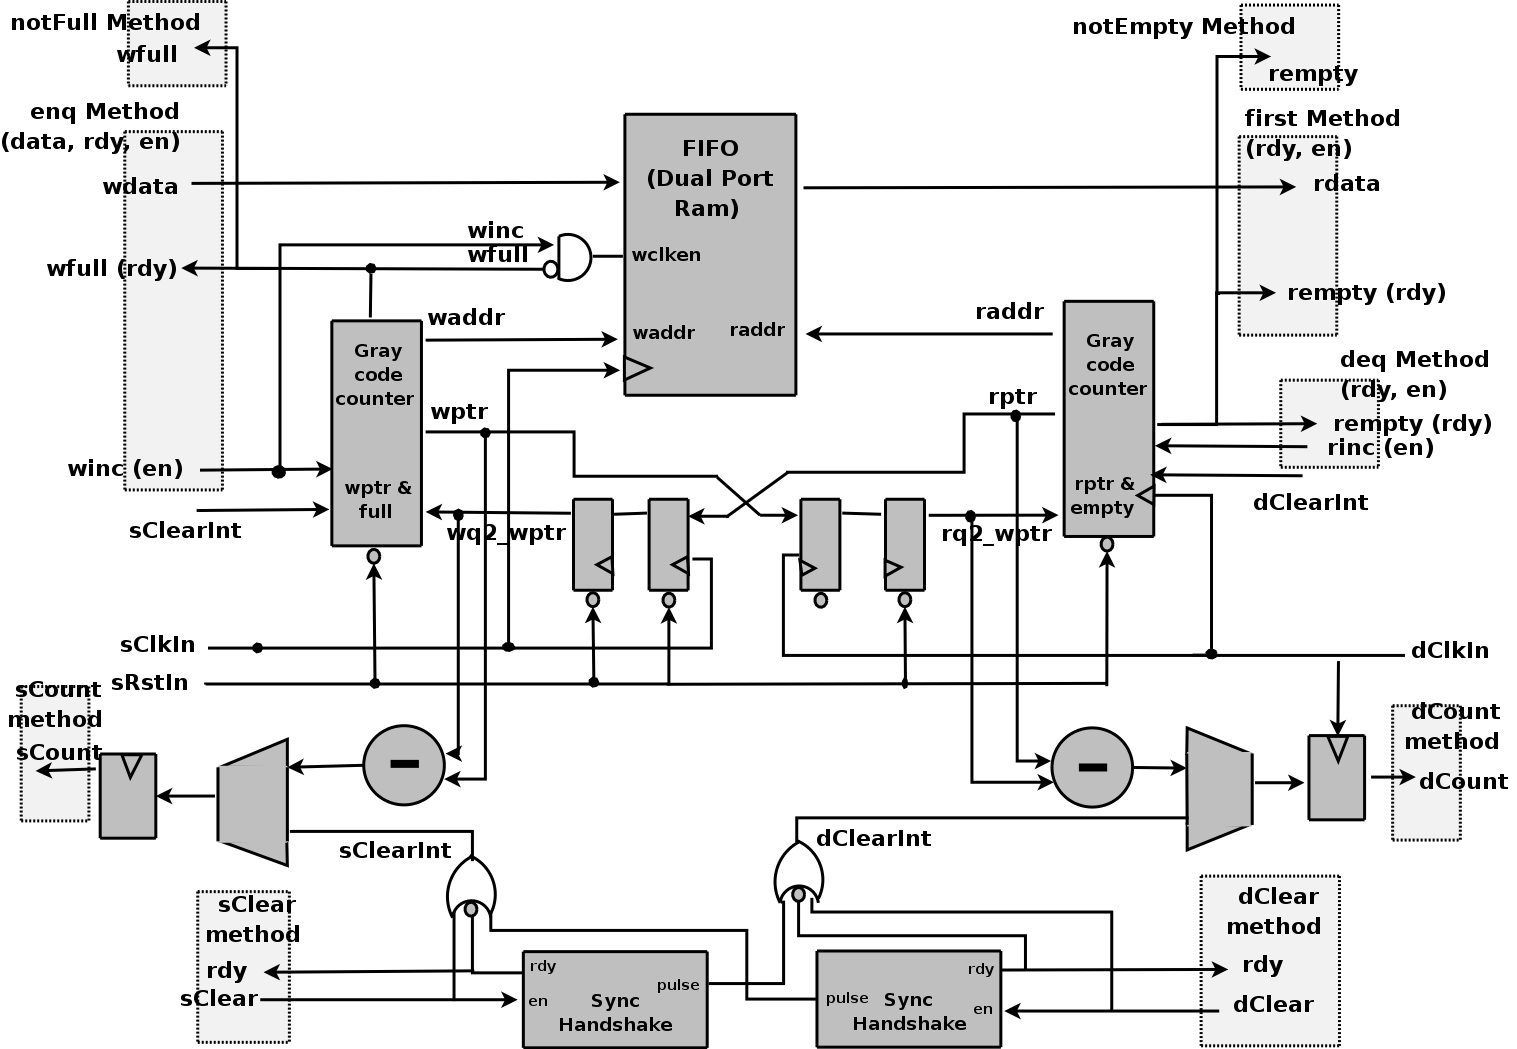
\includegraphics[width  = 5.5 in]{LibFig/syncfifocount}
\caption{SyncFIFOCount}
\label{syncfifocount}
\end{center}
\end{figure}


The module \te{mkSyncFIFOCount}, as shown in Figure
\ref{syncfifocount}  provides the \te{SyncFIFOCountIfc}
interface.  Because of the synchronization latency, the
count reports may  be different between the source
and the destination clocks.  Note
however, that the \te{sCount} and \te{dCount} reports give pessimistic
values with the appropriate side.  That is, the count \te{sCount} (on
the enqueue clock) will report the exact count of items in the FIFO or
a larger count.  The larger number is due to the 
synchronization delay in observing the dequeue action.  Likewise, the
\te{dCount} (on the dequeue clock) returns the exact count or a smaller
count.  The maximum disparity between \te{sCount} and \te{dCount}
depends on the difference in clock periods between the source and
destination clocks.

The module provides \te{sClear}  and \te{dClear}
methods, both of which cause the contents of the FIFO to be removed.
Since the clears must be synchronized and acknowledged from one domain
to the other, there is a non-trivial delay before the FIFO recovers
from the clear and can accept additional enqueues or dequeues
(depending on which side is cleared).  The calling of
either method immediately  disables other activity in the calling
domain. That is, calling \te{sClear} in cycle \te{n} causes the
enqueue to become unready in the next cycle, \te{n+1}.  Likewise, calling
\te{dClear} in cycle \te{n} causes the dequeue to become unready in
the next cycle, \te{n+1}.

%  That
% is, calling \te{sClear} in cycle \te{n} causes the method
% \te{sFull\_N} to return False (the Verilog port \te{sFULL\_N} is
% deasserted) and  \te{sCount} to return  $0$ in cycle \te{n+1}.
%  Further enqueues are disabled.  Likewise, calling \te{dClear} in
% cycle \te{n} causes the method \te{dEmpty\_N} to be asserted and \te{dCount} to
% be $0$ in cycle \te{n+1}.

After the \te{sClear} method is called, the FIFO appears empty on the
dequeue side after three \te{dClock} edges.  Three \te{sClock} edges later,
the FIFO returns to a state where new items can be enqueued.  The
latency is due to the full handshaking synchronization required to
send the clear signal to \te{dClock} and receive the acknowledgement back.

For the \te{dClear} method call, the enqueue side is cleared in three \te{sClkIn} edges and items can be enqueued at the fourth edge.  All
items enqueued at or before the clear are removed from the FIFO.

Note that there is a ready signal associated with both  \te{sClear}
and \te{dClear}
methods to ensure that the clear is properly sent between the clock
domains.  Also,  \te{sRstIn} must be synchronized with the \te{sClkIn}.

\begin{center}
\begin{tabular}{|p{1.1 in}|p{4.2 in}|}
 \hline
&         \\
Module Name  &  BSV Module Declaration  \\
\hline
\hline 
\te{mkSyncFIFOCount} 
& \begin{libverbatim}
module mkSyncFIFOCount( 
          Clock sClkIn, Reset sRstIn,
          Clock dClkIn,
          SyncFIFOCountIfc#(element_type, fifoDepth) ifc ) 
   provisos( Bits#(element_type, width_element));  
\end{libverbatim} 
\\
\cline{2-2}
&Comment: \te{width\_element} may be 0\\
\hline
\end{tabular}
\end{center}

%\end{itemize}
      
{\bf Example}
   
The following example shows the use of \te{SyncFIFOLevel} as a way
to collect data into a FIFO, and then send it out in a burst mode.  The
portion of the design shown, waits until the FIFO is almost
full, and then sets a register, {\tt burstOut} which indicates
that the FIFO should dequeue. When the FIFO is almost empty, the
flag is cleared, and FIFO fills again.

\begin{libverbatim}
   . . .
   // Define a fifo of Int(#23) with 128 entries
   SyncFIFOLevelIfc#(Int#(23),128) fifo <- mkSyncFIFOLevel(sclk, rst, dclk ) ;
  
   // Define some constants 
   let sFifoAlmostFull = fifo.sIsGreaterThan( 120 ) ;
   let dFifoAlmostFull = fifo.dIsGreaterThan( 120 ) ;
   let dFifoAlmostEmpty = fifo.dIsLessThan( 12 ) ;
  
   // a register to indicate a burst mode
   Reg#(Bool)  burstOut <- mkReg( False, clocked_by (dclk)) ;
  
   . . .
   // Set and clear the burst mode depending on fifo status
   rule timeToDeque( dFifoAlmostFull && ! burstOut ) ;
      burstOut <= True ;
   endrule
  
  
   rule moveData ( burstOut ) ;
      let dataToSend = fifo.first ;
      fifo.deq ;
      ...
      burstOut <= !dFifoAlmostEmpty;

   endrule
\end{libverbatim}


{\bf Scheduling Annotations}

Scheduling constraints describe how methods interact within the
schedule.
The annotations for \te{mkFIFOLevel} and \te{mkSyncFIFOLevel} are the
same, except that 
methods in different domains (source and destination) are always
conflict free.


\begin{center}
\begin{tabular}{|c|c|c|c|c|c|c|c|c|}
%begin{tabular}{|p{.75 in}|c|c|c|c|}
\hline
\multicolumn{9}{|c|}{Scheduling Annotations}\\
\multicolumn{9}{|c|}{\te{mkFIFOLevel}, \te{mkSyncFIFOLevel}}\\
\hline
&enq&first&deq&clear&notFull&notEmpty&isLessThan&isGreaterThan\\
\hline
\hline
enq&C &CF&CF&SB&SA&SA&SA&SA\\
\hline
first&CF&CF&SB&SB&CF&CF&CF&CF\\
\hline
deq&CF &SA&C&SB&SA&SA&SA&SA\\
\hline
clear&SA&SA&SA&SBR&SA&SA&SA&SA\\
\hline
notFull&SB&CF&SB&SB&CF&CF&CF&CF\\
\hline
notEmpty&SB&CF&SB&SB&CF&CF&CF&CF\\
\hline
isLessThan&SB&CF&SB&SB&CF&CF&CF&CF\\
\hline
isGreaterThan&SB&CF&SB&SB&CF&CF&CF&CF\\
\hline
\hline
\end{tabular}
\end{center}

The annotations for \te{mkFIFOCount} and \te{mkSyncFIFOCount} are the
same, except that 
methods in different domains (source and destination) are always
conflict free.


\begin{center}
\begin{tabular}{|c|c|c|c|c|c|c|c|}
\hline
\multicolumn{8}{|c|}{Scheduling Annotations}\\
\multicolumn{8}{|c|}{\te{mkFIFOCount}, \te{mkSyncFIFOCount}}\\
\hline
&enq&first&deq&clear&notFull&notEmpty&count\\
\hline
\hline
enq&C&CF&CF&SB&SA&SA&SA\\
\hline
first&CF &CF&SB&SB&CF&CF&CF\\
\hline
deq&CF &SA&C&SB&SA&SA&SA\\
\hline
clear&SA&SA&SA&SBR&SA&SA&SA\\
\hline
notFull&SB&CF&SB&SB&CF&CF&CF\\
\hline
notEmpty&SB&CF&SB&SB&CF&CF&CF\\
\hline
count&SB&CF&SB&SB&CF&CF&CF\\
\hline
\hline
\end{tabular}
\end{center}






{\bf Verilog Modules}

The modules described in this section  correspond to the following {\V}
modules, which are found in the BSC {\V} library,
\te{\$BLUESPECDIR/Verilog/}.  

\begin{center}
\begin{tabular} {|p{2 in}|p{1.5 in}p{1.5 in}|}
\hline
&& \\
BSV Module Name &\multicolumn{2}{|c|}{ Verilog Module Names}  \\
&& \\
\hline
\hline
\begin{libverbatim}mkFIFOLevel
mkFIFOCount
\end{libverbatim}
& \te{SizedFIFO.v} & \te{SizedFIFO0.v} \\
\hline
\begin{libverbatim}mkSyncFIFOLevel
mkSyncFIFOCount
\end{libverbatim}
&\te{SyncFIFOLevel.v}&\\
\hline
\end{tabular}
\end{center}



\subsubsection{BRAMFIFO}
\label{sec-BRAMFIFO}
%\index{Xilinx!BRAMFIFO (package)}

{\bf Package}
\index{BRAMFIFO (package)}

\begin{verbatim}
import BRAMFIFO :: * ;
\end{verbatim}




{\bf Description}

The \te{BRAMFIFO} package provides FIFO interfaces and are built
around a BRAM memory. The BRAM is provided in the \te{BRAMCore} 
package described in Section \ref{sec-BRAMCore}.  


{\bf Interfaces}

The \te{BRAMFIFO} package provides \te{FIFOF}, \te{FIFO}, and
\te{SyncFIFOIfc} interfaces, as defined in the \te{FIFOF}, \te{FIFO},
(both in Section \ref{sec-FIFOifc}) 
and \te{Clocks} (Section \ref{syncfifoifc}) packages.


{\bf Modules}


\index{mkSizedBRAMFIFOF@\te{mkSizedBRAMFIFOF} (module)}
\index[function]{BRAMFIFO!mkSizedBRAMFIFOF}

\begin{tabular}{|p{1.4 in}|p{4.2 in}|}
\hline
& \\
\te{mkSizedBRAMFIFOF} &Provides a \te{FIFOF} interface of a given depth, \te{n}.\\
\cline{2-2}
& \begin{libverbatim}
module mkSizedBRAMFIFOF#(Integer n) (FIFOF#(element_type))
   provisos (Bits(element_type, width_any), 
             Add#(1,z,width_any));
\end{libverbatim}
\\
\hline
\end{tabular}

\index{mkSizedBRAMFIFO@\te{mkSizedBRAMFIFO} (module)}
\index[function]{BRAMFIFO!mkSizedBRAMFIFO}

\begin{tabular}{|p{1.4 in}|p{4.2 in}|}
\hline
& \\
\te{mkSizedBRAMFIFO} &Provides a \te{FIFO} interface of a given
depth, \te{n}.\\
\cline{2-2}
& \begin{libverbatim}
module mkSizedBRAMFIFO#(Integer n)(FIFO#(element_type))
   provisos(Bits#(t, width_element),
            Add#(1, z, width_element) );
\end{libverbatim}
\\
\hline
\end{tabular}

\index{mkSyncBRAMFIFO@\te{mkSyncBRAMFIFO} (module)}
\index[function]{BRAMFIFO!mkSyncBRAMFIFO}

\begin{tabular}{|p{1.4 in}|p{4.2 in}|}
\hline
& \\
\te{mkSyncBRAMFIFO}  &Provides a \te{SyncFIFOIfc} interface to send
data across clock domains.  The \te{enq} method is in the source
\te{sClkIn} domain, while the \te{deq} and \te{first} methods are in
the destination \te{dClkIn} domain.  The input and output clocks,
along with the input and output resets, are explicitly provided.  The
default clock and reset are ignored.\\
\cline{2-2}
& \begin{libverbatim}
module mkSyncBRAMFIFO#(Integer depth, 
                       Clock sClkIn, Reset sRstIn, 
                       Clock dClkIn, Reset dRstIn)
                       (SyncFIFOIfc#(element_type))
   provisos(Bits#(element_type, width_element),
            Add#(1, z, width_element));
\end{libverbatim}
\\
\hline
\end{tabular}

\index{mkSyncBRAMFIFOToCC@\te{mkSyncBRAMFIFOToCC} (module)}
\index[function]{BRAMFIFO!mkSyncBRAMFIFOToCC}

\begin{tabular}{|p{1.4 in}|p{4.2 in}|}
\hline
& \\
\te{mkSyncBRAMFIFOToCC} &Provides a \te{SyncFIFOIfc} interface to send
data from a second clock domain into the current clock domain.  The
output clock and reset are the current clock and reset. \\
\cline{2-2}
& \begin{libverbatim}
module mkSyncBRAMFIFOToCC#(Integer depth, 
                           Clock sClkIn, Reset sRstIn)
                           (SyncFIFOIfc#(element_type))
   provisos(Bits#(element_type, width_element),
            Add#(1, z, width_element));
\end{libverbatim}
\\
\hline
\end{tabular}

\index{mkSyncBRAMFIFOFromCC@\te{mkSyncBRAMFIFOFromCC} (module)}
\index[function]{BRAMFIFO!mkSyncBRAMFIFOFromCC}

\begin{tabular}{|p{1.4 in}|p{4.2 in}|}
\hline
& \\
\te{mkSyncBRAMFIFOFromCC} &Provides a  \te{SyncFIFOIfc} interface to send
data from the current clock domain into a second clock domain.  The
input clock and reset are the current clock and reset.  \\
\cline{2-2}
& \begin{libverbatim}
module mkSyncBRAMFIFOFromCC#(Integer depth, 
                             Clock dClkIn, Reset dRstIn)
                             (SyncFIFOIfc#(element_type))
   provisos(Bits#(element_type, width_element),
            Add#(1, z, width_element));
\end{libverbatim}
\\
\hline
\end{tabular}

\subsubsection{SpecialFIFOs}
 
\index{SpeciaFIFOs@\te{SpecialFIFOs} (package)}

\label{sec-SpecialFIFOs}

{\bf Package}

\begin{verbatim}
import SpecialFIFOs :: * ;
\end{verbatim}







{\bf Description}

The SpecialFIFOs package contains various FIFOs provided as BSV source
code, allowing users to easily modify them to their own
specifications.  Included in the  SpecialFIFOs package are pipeline
and bypass FIFOs.   The pipeline
FIFOs are equivalent to the \te{mkLFIFO} (Section
\ref{sec-fifo-mod}); they allow simultaneous enqueue and dequeue
operations in the same clock cycle when {\em full}.  The bypass FIFOs allow
simultaneous enqueue and dequeue in the same clock cycle when {\em
empty}. FIFOF versions, with explicit full and empty signals, are
provided for both pipeline and bypass FIFOs.  The package also
includes the \te{DFIFOF}, a FIFOF with unguarded dequeue and first
methods (thus they have no implicit conditions).

\begin{center}
\begin{tabular}{|p {1.3 in}|p{.8 in}|p {3.2 in}|}
\hline
\multicolumn{3}{|c|}{FIFOs in Special FIFOs package}\\
\hline
\hline
Module name& Interface&Description \\
\hline
\te{mkPipelineFIFO}&\te{FIFO}&1 element pipeline FIFO;  can \te{enq}
and \te{deq} simultaneously when full.\\
\hline
\te{mkPipelineFIFOF}&\te{FIFOF}&1 element pipeline FIFO with explicit full and empty signals. \\
\hline
\te{mkBypassFIFO}&\te{FIFO}&1 element bypass FIFO;  can  \te{enq} and
\te{deq} simultaneously when empty.\\
\hline
\te{mkBypassFIFOF}&\te{FIFOF}&1 element bypass FIFO with explicit full and empty signals.\\
\hline
\te{mkSizedBypassFIFOF} &\te{FIFOF}&Bypass FIFO of given depth, with
explicit full and empty signals.\\
\hline
\te{mkBypassFIFOLevel}&\te{FIFOLevelIfc}&Same as a \te{FIFOLevel}
(Section \ref{FIFOLevel}), but can \te{enq} and \te{deq} when empty.\\
\hline
\te{mkDFIFOF}&\te{FIFOF}&A FIFOF with unguarded \te{deq} and
\te{first} methods where the \te{first} method returns specified
default value when the FIFO is empty.\\
\hline
\hline
\end{tabular}
\end{center}

\begin{center}
\begin{tabular}{|p{2 in}|c|c|c|}
\hline
\multicolumn{4}{|c|}{Allowed Simultaneous enq and deq}\\
\multicolumn{4}{|c|}{by FIFO type}\\
\hline
&\multicolumn{3}{|c|}{FIFO Condition}\\
\cline{2-4}
FIFO type&empty&not empty&full\\
&&not full &\\
\hline
\hline
\te{mkPipelineFIFO}&&NA&$\surd$\\
\te{mkPipelineFIFOF}&&&\\
\hline
\te{mkBypassFIFO}&$\surd$&NA&\\
\te{mkBypassFIFOF}&&&\\
\hline
\te{mkSizedBypassFIFOF}&$\surd$&$\surd$&\\
\hline
\te{mkBypassFIFOLevel}&$\surd$&$\surd$&\\
\hline
\te{mkDFIFOF}&$\surd$&$\surd$&$\surd$\\
\hline
\hline
\end{tabular}
\end{center}


{\bf Interfaces and methods} 

The modules defined in the \te{SpecialFIFOs} package provide the
\te{FIFO}, \te{FIFOF}, and 
\te{FIFOLevelIfc} interfaces, as shown in the table above.  These
interfaces are described in Section \ref{sec-FIFO} (FIFO package)
and Section \ref{FIFOLevel} (FIFOLevel package). 



{\bf Modules}
\index{mkPipelineFIFO@\te{mkPipelineFIFO} (module)}
\index[function]{SpecialFIFOs!mkPipelineFIFO}


\begin{center}
\begin{tabular}{|p{1.4 in}|p{4.1 in}|}
 \hline
  &            \\
Module Name  &  BSV Module Declaration   \\
\hline
\multicolumn{2}{|l|}{1-element pipeline FIFO; can \te{enq} and
  \te{deq} simultaneously when full.}\\
\hline
\begin{libverbatim}mkPipelineFIFO 
\end{libverbatim} 
& \begin{libverbatim}
module mkPipelineFIFO (FIFO#(element_type))
   provisos (Bits#(element_type, width_any));
 \end{libverbatim} 
\\
\hline
\end{tabular}
\end{center}

\index{mkPipelineFIFOF@\te{mkPipelineFIFOF} (module)}
\index[function]{SpecialFIFOs!mkPipelineFIFOF}


\begin{center}
\begin{tabular}{|p{1.4 in}|p{4.1 in}|}
 \hline
\multicolumn{2}{|l|}{1-element pipeline FIFOF; can \te{enq} and
  \te{deq} simultaneously when full.}\\
\multicolumn{2}{|l|}{Has explicit full and empty signals.}\\
\hline
\begin{libverbatim}mkPipelineFIFOF 
\end{libverbatim} 
& \begin{libverbatim}
module mkPipelineFIFOF (FIFOF#(element_type))
   provisos (Bits#(element_type, width_any));
 \end{libverbatim} 
\\
\hline
\end{tabular}
\end{center}

\index[function]{SpecialFIFOs!mkBypassFIFO}
\index[function]{SpecialFIFOs!mkBypassFIFOF}
\index{mkBypassFIFO@\te{mkBypassFIFO} (module)}
\index{mkBypassFIFOF@\te{mkBypassFIFOF} (module)}

\begin{center}
\begin{tabular}{|p{1.4 in}|p{4.1 in}|}
 \hline
\multicolumn{2}{|l|}{1-element bypass FIFO; can \te{enq} and \te{deq}
simultaneously when empty.}\\
\hline
\begin{libverbatim}mkBypassFIFO 
\end{libverbatim} 
& \begin{libverbatim}
module mkBypassFIFO (FIFO#(element_type))
   provisos (Bits#(element_type, width_any));
 \end{libverbatim} 
\\
\hline
\end{tabular}
\end{center}

\begin{center}
\begin{tabular}{|p{1.4 in}|p{4.1 in}|}
 \hline
\multicolumn{2}{|l|}{1-element bypass FIFOF;  can \te{enq} and \te{deq}
simultaneously when empty.}\\
\multicolumn{2}{|l|}{Has explicit full and empty signals.}\\
\hline
\begin{libverbatim}mkBypassFIFOF 
\end{libverbatim} 
& \begin{libverbatim}
module mkBypassFIFOF (FIFOF#(element_type))
   provisos (Bits#(element_type, width_any));
 \end{libverbatim} 
\\
\hline
\end{tabular}
\end{center}


\index{mkSizedBypassFIFOF@\te{mkSizedBypassFIFOF} (module)}
\index[function]{SpecialFIFOs!mkSizedBypassFIFOF}

\begin{center}
\begin{tabular}{|p{1.4 in}|p{4.1 in}|}
 \hline
\multicolumn{2}{|l|}{Bypass FIFOF of given depth \te{fifoDepth} with 
explicit full and empty signals.}\\ 
\hline
\begin{libverbatim}mkSizedBypassFIFOF 
\end{libverbatim} 
& \begin{libverbatim}
module mkSizedBypassFIFOF#(Integer fifoDepth)
                          (FIFOF#(element_type))
   provisos (Bits#(element_type, width_any));
 \end{libverbatim} 
\\
\hline
\end{tabular}
\end{center}


\index{mkBypassFIFOLevel@\te{mkBypassFIFOLevel} (module)}
\index[function]{SpecialFIFOs!mkBypassFIFOLevel}

\begin{center}
\begin{tabular}{|p{1.4 in}|p{4.1 in}|}
 \hline
\multicolumn{2}{|l|}{Bypass FIFOLevel of given depth \te{fifoDepth}}\\
\hline
\begin{libverbatim}mkBypassFIFOLevel 
\end{libverbatim} 
& \begin{libverbatim}
module mkBypassFIFOLevel(FIFOLevelIfc#(element_type, 
                                       fifoDepth))
   provisos( Bits#(element_type, width_any), 
   Log#(TAdd#(fifoDepth,1), cntSize));
 \end{libverbatim} 
\\
\hline
\end{tabular}
\end{center}

\index{mkDFIFOF@\te{mkDFIFOF} (module)}
\index[function]{SpecialFIFOs!mkDFIFOF}

\begin{center}
\begin{tabular}{|p{1.4 in}|p{4.1 in}|}
 \hline
\multicolumn{2}{|l|}{A FIFOF with unguarded \te{deq} and \te{first}
methods (thus they have no implicit conditions).}\\
\multicolumn{2}{|l|}{The \te{first} method
returns a specified default value when the FIFO is empty}\\
\hline
\begin{libverbatim}mkDFIFOF 
\end{libverbatim} 
& \begin{libverbatim}
module mkDFIFOF#(element_type default_value) 
                (FIFOF#(element_type))
   provisos (Bits#(element_type, width_any));
 \end{libverbatim} 
\\
\hline
\end{tabular}
\end{center}


% {\bf Scheduling Annotations}

% Scheduling constraints describe how methods interact within the schedule.
%   For example, a \te{clear} to a given
% FIFO must be sequenced after (\te{SA}) an \te{enq} to the same
%   FIFO.  That is, when both \te{enq} and \te{clear} execute in the same
%   cycle, the resulting FIFO state is empty.  For correct rule behavior
%   the rule executing \te{enq} must be scheduled before the rule
%   calling \te{clear}.  

% The  table below lists the scheduling annotations for the FIFO modules
% \te{mkFIFO}, \te{mkSizedFIFO}, and \te{mkFIFO1}.

% \begin{center}
% %\begin{tabular}{|p{.75 in}|p{.75 in}|p{.75 in}|p{.75 in}|p{.75 in}|}
% \begin{tabular}{|p{.75 in}|c|c|c|c|}
% \hline
% \multicolumn{5}{|c|}{Scheduling Annotations}\\
% \multicolumn{5}{|c|}{mkFIFO, mkSizedFIFO, mkFIFO1}\\
% \hline
% &enq&first&deq&clear\\
% \hline
% \hline
% enq&C &CF&CF&SB\\
% \hline
% first&CF&CF&SB&SB\\
% \hline
% deq&CF&SA&C&SB\\
% \hline
% clear&SA&SA&SA&SBR\\
% \hline
% \hline
% \end{tabular}
% \end{center}

% The  table below lists the scheduling annotations for the pipeline
% FIFO module, \te{mkLFIFO}.  The pipeline FIFO has a few more
% restrictions since there is a combinational path between the \te{deq}
% side and the \te{enq} side, thus restricting \te{deq} calls before \te{enq}.

% \begin{center}
% \begin{tabular}{|p{.75 in}|c|c|c|c|}
% \hline
% \multicolumn{5}{|c|}{Scheduling Annotations}\\
% \multicolumn{5}{|c|}{mkLFIFO}\\
% \hline
% &enq&first&deq&clear\\
% \hline
% \hline
%  enq&C &SA&SAR&SB\\
% \hline
%  first&SB&CF&SB&SB\\
% \hline
%  deq&SBR&SA&C&SB\\
% \hline
%  clear&SA&SA&SA&SBR\\
% \hline
% \hline
% \end{tabular}
% \end{center}

% The \te{FIFOF} modules add the \te{notFull} and \te{notEmpty}
% methods. These methods have SB annotations with the Action methods
% that change FIFO state.  These SB annotations model  the atomic
% behavior of a  FIFO, that
% is when \te{enq}, \te{deq}, or \te{clear} are called the state of
% \te{notFull} and \te{notEmpty} are changed.  This is no different than
% the annotations on \te{mkReg} (which is \te{read} SB \te{write}),
% where actions are atomic and the execution module is one rule fires at
% a time.  This does differ from a pure hardware module of a FIFO or
% register where the state does not change until the clock edge.

% \begin{center}
% \begin{tabular}{|p{.75 in}|c|c|c|c|c|c|}
% \hline
% \multicolumn{7}{|c|}{Scheduling Annotations}\\
% \multicolumn{7}{|c|}{mkFIFOF, mkSizedFIFOF, mkFIFOF1}\\
% \hline
% &enq&notFull&first&deq&notEmpty&clear\\
% \hline
% \hline
%  enq&C &SA&CF&CF&SA&SB\\
% \hline
%  notFull&SB&CF&CF&SB&CF&SB\\
% \hline
%  first&CF&CF&CF&SB&CF&SB\\
% \hline
%  deq&CF&SA&SA&C&SA&SB\\
% \hline
%  notEmpty&SB&CF&CF&SB&CF&SB\\
% \hline
%  clear&SA&SA&SA&SA&SA&SBR\\
% \hline
% \hline
% \end{tabular}
% \end{center}



% {\bf Verilog Modules}

% \te{FIFO} and \te{FIFOF} modules correspond to the following {\V}
% modules, which are found in the BSC {\V} library, \te{\$BLUESPECDIR/Verilog/}.

% \begin{center}
% \begin{tabular} {|p{1.5in}|p{1in}p{1 in}|p{1.8 in}|}
% \hline
% &&& \\
% BSV Module Name &\multicolumn{2}{|c|}{ Verilog Module Names}&Comments  \\
% &&& \\
% \hline
% \hline
% \begin{libverbatim}mkFIFO
% mkFIFOF
% mkUGFIFOF
% mkGFIFOF\end{libverbatim}
% & \te{FIFO2.v}&   \te{FIFO20.v}&\\
% \hline
% \end{tabular}

% \begin{tabular} {|p{1.5in}|p{1in}p{1 in}|p{1.8 in}|}
% \hline
% \begin{libverbatim}mkFIFO1
% mkFIFOF1
% mkUGFIFOF1
% mkGFIFOF1\end{libverbatim} 
% & \te{FIFO1.v} & \te{FIFO10.v}&\\
% \hline
% \end{tabular}

% \begin{tabular} {|p{1.5in}|p{1in}p{1 in}|p{1.8 in}|}
% \hline
% \begin{libverbatim}mkSizedFIFO
% mkSizedFIFOF
% mkUGSizedFIFOF
% mkGSizedFIFOF
% \end{libverbatim} 
% &\begin{libverbatim}SizedFIFO.v
% FIFO1.v
% FIFO2.v
% \end{libverbatim}
%  & \begin{libverbatim}SizedFIFO0.v
% FIFO10.v
% FIFO20.v
% \end{libverbatim}
% &If the depth of the FIFO = 1,
% then \te{FIFO1.v} and \te{FIFO10.v} are used, if the depth = 2, then
% \te{FIFO2.v} and \te{FIFO20.v} are used. \\
% \hline
% \end{tabular}

% \begin{tabular} {|p{1.5in}|p{1in}p{1 in}|p{1.8 in}|}
% \hline
% \begin{libverbatim}
% mkDepthParamFIFOF
% mkUGDepthParamFIFOF
% mkGDepthParamFIFOF\end{libverbatim} 
% & \te{SizedFIFO.v} & \te{SizedFIFO0.v}& \\
% \hline
% \end{tabular}

% \begin{tabular} {|p{1.5in}|p{1in}p{1 in}|p{1.8 in}|}
% \hline
% \begin{libverbatim}mkLFIFO
% mkLFIFOF
% mkUGLFIFOF
% mkGLFIFOF\end{libverbatim}
%  & \te{FIFOL1.v} &  \te{FIFOL10.v}& \\
% \hline
% \hline
% \end{tabular}
% \end{center}
 

% % Text inserted here to explain anything the user might need to know
% % about how the Verilog relates to the BSV they wrote.


\subsubsection{AlignedFIFOs}
 
\index{AlignedFIFOs@\te{AlignedFIFOs} (package)}

\label{sec-AlignedFIFOs}

{\bf Package}

\begin{verbatim}
import AlignedFIFOs :: * ;
\end{verbatim}





{\bf Description}

The AlignedFIFOs package contains a parameterized FIFO module
intended for creating synchronizing FIFOs between clock domains
with aligned edges for both types of clock domain crossings:
\begin{itemize}
\item slow-to-fast crossing - every edge in the source domain implies
the existence of a simultaneous edge in the destination domain 
\item fast-to-slow crossing - every edge in the destination domain
implies the existence of a simultaneous edge in the source domain
\end{itemize}

The FIFO is parameterized on the type of store used to hold the
FIFO data, which is itself parameterized on the index type, value
type, and read latency.  Modules to construct stores based on a
single register, a vector of registers and a BRAM are provided, and
the user can supply their own store implementation as well.

The FIFO allows the user to control whether or not outputs are held
stable during the full slow clock cycle or allowed to transition
mid-cycle.  Holding the outputs stable is the safest option but it
 slightly increases the minimum latency through the FIFO.

A primary design goal of this FIFO is to provide an efficient
and flexible family of synchronizing FIFOs between aligned clock
 domains which are written in BSV and are fully compatible with
 Bluesim.  These FIFOs (particularly ones using vectors of registers)
 may not be the best choice for ASIC synthesis due to the muxing
 to select the head value in the \te{first} method.



{\bf Interfaces and methods} 



\paragraph{Store Interface}
The \te{AlignedFIFO} is parameterized on the type of store used to hold the FIFO
data. The three types of
stores provided in the \te{AlignedFIFO} package (single-element,
vector-of-registers, and BRAM) all return a \te{Store} interface.

The \te{Store} interface has a \te{prefetch} method which is used by
some modules (the \te{mkBRAMStore} in this package).   If a prefetch
is used, the \te{read} 
method returns the value at the previously fetched index; the
value of \te{idx} should be ignored.   If a prefetch is not
used, the \te{read} method index value determines the returned
value. 

% \begin{center}
% \begin{tabular}{|p{.4 in}|p{1.5 in}|p{.4in}| p{2 in}|}
% \hline
% \multicolumn{4}{|c|}{Type parameters used in Interfaces}\\
% \hline
% Name&Description&Valid Values&\\
% \hline
% \te{i}& data type of index&&\\
% \hline
% \te{a} &data type of values in FIFO&&\\
% \hline
% \te{n}& Read latency & 0& prefetch is not used   \\
% \cline{3-4}
% && 1&  prefetch is used\\
% \hline
% \end{tabular}
% \end{center}




\begin{center}
\begin{tabular}{|p{1.1in}|p{.4in}|p{3.5 in}|}
\hline
\multicolumn{3}{|c|}{Store Interface Methods}\\
\hline
Name & Type & Description\\
\hline
\hline 
\te{write}&Action&Writes the value at index \te{idx}.\\
\hline
\te{prefetch}&Action&Initiates a prefetch of the value at index \te{idx}. \\
\hline
\te{read}&\te{a}&Returns the value of type \te{a}.  If prefetch is not
used,  returns the value at index \te{idx}.  When prefetch is used,
returns the value at the previously fetched index; the value of \te{idx} should be ignored.\\ 
\hline
\end{tabular}
\end{center}


\begin{verbatim}
interface Store#(type i, type a, numeric type n);
   method Action write(i idx, a value);
   method Action prefetch(i idx);
   method a read(i idx);
endinterface: Store
\end{verbatim}


\paragraph{AlignedFIFO Interface}

The \te{AlignedFIFO} interface provides methods for both source (enqueue) and
destination (dequeue) clock domains.  

\begin{center}
\begin{tabular}{|p{1.1in}|p{.4in}|p{3.5 in}|}
\hline
\multicolumn{3}{|c|}{AlignedFIFO Interface Methods}\\
\hline
\hline
Name&Type&Description\\
\hline
\hline
\te{enq}&Action&Adds an entry to the FIFO from the source clock domain.\\
\hline
\te{first}&\te{a}&Returns the first entry from the FIFO in the
destination clock domain.\\
\hline
\te{deq}&Action&Removes the first entry from the FIFO in the
destination clock domain.\\
\hline
\te{dNotFull}&Bool&Returns \te{True} if the FIFO appears not full from
the destination  clock domain.\\
\hline
\te{dNotEmpty}&Bool&Returns \te{True} if the FIFO appears not empty from
the destination  clock domain.\\
\hline
\te{sNotFull}&Bool&Returns \te{True} if the FIFO appears not full from
the source  clock domain.\\
\hline
\te{sNotEmpty}&Bool&Returns \te{True} if the FIFO appears not empty from
the source  clock domain.\\
\hline
\te{dClear}&Action&Clears the FIFO from the destination side.\\
\hline
\te{sClear}&Action&Clears the FIFO from the source side.\\
\hline
\end{tabular}
\end{center}

\begin{verbatim}
interface AlignedFIFO#(type a);
   method Action enq(a x);
   method a first();
   method Action deq();
   method Bool dNotFull();
   method Bool dNotEmpty();
   method Bool sNotFull();
   method Bool sNotEmpty();
   method Action dClear();
   method Action sClear();
endinterface: AlignedFIFO
\end{verbatim}




{\bf Modules}

 The
\te{AlignedFIFO} module  is  parameterized on the type of store used to hold
the FIFO data.  The \te{AlignedFIFOs} package contains modules to
construct stores based on a single register (\te{mkRegStore}), a
vector of registers (\te{mkRegVectorStore}), and a BRAM (\te{mkBRAMStore}). 
Users can supply their own store implementation as well.

\index{mkRegStore@\te{mkRegStore} (module)}
\index[function]{AlignedFIFOs!mkRegStore}

The \te{mkRegStore} instantiates a  single-element store.  The module returns
a \te{Store} interface and does not use a prefetch.

\begin{center}
\begin{tabular}{|p{1.4 in}|p{4.1 in}|}
 \hline
  &            \\
Module Name  &  BSV Module Declaration   \\
\hline
\multicolumn{2}{|l|}{Implementation of a single-element store }\\
\hline
\begin{libverbatim}mkRegStore
\end{libverbatim} 
& \begin{libverbatim}
module mkRegStore(Clock sClock, Clock dClock, 
                  Store#(UInt#(0),a,0) ifc)
   provisos(Bits#(a,a_sz) ); \end{libverbatim} 
\\
\hline
\end{tabular}
\end{center}

\index{mkRegVectorStore@\te{mkRegVectorStore} (module)}
\index[function]{AlignedFIFOs!mkRegVectorStore}

The \te{mkRegVectorStore} module instantiates a vector-of-registers
store.  The module returns a \te{Store} interface and does not use a
prefetch.

\begin{center}
\begin{tabular}{|p{1.4 in}|p{4.1 in}|}
 \hline
\multicolumn{2}{|l|}{Implementation of a vector-of-registers store}\\
\hline
\begin{libverbatim}mkRegVectorStore
\end{libverbatim} 
& \begin{libverbatim}
module mkRegVectorStore(Clock sClock, Clock dClock, 
                        Store#(UInt#(w),a,0) ifc)
   provisos( Bits#(a,a_sz) ); \end{libverbatim} 
\\
\hline
\end{tabular}
\end{center}

\index{mkBRAMStore2W1R@\te{mkBRAMStore2W1R} (module)}
\index[function]{AlignedFIFOs!mkBRAMStore2W1R}

The \te{mkBRAMStore2W1R} module returns a \te{Store} interface and uses a
prefetch.  This model assumes the read clock is a 2x divided version
of the write clock.

\begin{center}
\begin{tabular}{|p{1.4 in}|p{4.1 in}|}
 \hline
\multicolumn{2}{|l|}{A BRAM-based store where the
read clock is a 2x divided version of the write clock.}\\
\hline
\begin{libverbatim}mkBRAMStore2W1R
\end{libverbatim} 
& \begin{libverbatim}
module mkBRAMStore2W1R(Clock sClock, Reset sReset, 
                       Clock dClock, Reset dReset, 
                       Store#(i,a,1) ifc)
   provisos( Bits#(a,a_sz), Bits#(i,w), Eq#(i) );\end{libverbatim}
\\
\hline
\end{tabular}
\end{center}

\index{mkBRAMStore1W2R@\te{mkBRAMStore1W2R} (module)}
\index[function]{AlignedFIFOs!mkBRAMStore1W2R}

The \te{mkBRAMStore1W2R} module returns a \te{Store} interface and uses a
prefetch.  This model assumes the write clock is a 2x divided version
of the read clock.

\begin{center}
\begin{tabular}{|p{1.4 in}|p{4.1 in}|}
 \hline
\multicolumn{2}{|l|}{A BRAM-based store where the
write clock is a 2x divided version of read clock.}\\
\hline
\begin{libverbatim}mkBRAMStore1W2R
\end{libverbatim} 
& \begin{libverbatim}
module mkBRAMStore1W2R(Clock sClock, Reset sReset, 
                       Clock dClock, Reset dReset, 
                       Store#(i,a,1) ifc)
   provisos( Bits#(a,a_sz), Bits#(i,w), Eq#(i) );\end{libverbatim}
\\
\hline
\end{tabular}
\end{center}

\index{mkAlignedFIFO@\te{mkAlignedFIFO} (module)}
\index[function]{AlignedFIFOs!mkAlignedFIFO}

The \te{mkAlignedFIFO} module makes a synchronizing FIFO for aligned
clocks, based on the given backing store (determined by the type of
store instantiated).  The store is assumed to have $2^{w}$ slots
addressed from 0 to $2^{w}-1$.  The store will be written in the
source clock domain and read in the destination clock domain.

The \te{enq} and \te{deq} methods will only be callable when the
\te{allow\_enq} and \te{allow\_deq} inputs are high.  For a
slow-to-fast crossing use:
\begin{libverbatim}
allow_enq = constant True
allow_deq = pre-edge signal
\end{libverbatim}

For a fast-to-slow crossing, use:
\begin{libverbatim}
allow_enq = pre-edge signal
allow_deq = constant True
\end{libverbatim}

The pre-edge signal is \te{True} when the slow clock will rise in the
next clock cycle.   The
\te{ClockNextRdy}  from the \te{ClockDividerIfc} (Section
\ref{sec-clockdivider}) can be used as the pre-edge signal.

These settings ensure that the outputs in the slow clock domain are
stable for the entire cycle.  Setting both inputs to constant True
reduces the minimum latency through the FIFO, but allows outputs in
the slow domain to transition mid-cycle.  This is less safe and can
interact badly with the \te{\$displays} in a Verilog simulation.


It is not advisable to call both \te{dClear} and \te{sClear} simultaneously.

\begin{center}
\begin{tabular}{|p{1.4 in}|p{4.1 in}|}
 \hline
\multicolumn{2}{|l|}{Implementation of an aligned FIFO}\\
\hline
\begin{libverbatim}mkAlignedFIFO
\end{libverbatim} 
& \begin{libverbatim}
(* no_default_clock, no_default_reset *)
module mkAlignedFIFO( Clock sClock
		    , Reset sReset
		    , Clock dClock
		    , Reset dReset
		    , Store#(i,a,n) store
		    , Bool allow_enq
		    , Bool allow_deq
		    , AlignedFIFO#(a) ifc
		    )
   provisos( Bits#(a,sz_a), Bits#(i,w), 
             Eq#(i), Arith#(i) );\end{libverbatim}
\\
\hline
\end{tabular}
\end{center}



% {\bf Verilog Modules}

% \te{FIFO} and \te{FIFOF} modules correspond to the following {\V}
% modules, which are found in the BSC {\V} library, \te{\$BLUESPECDIR/Verilog/}.

% \begin{center}
% \begin{tabular} {|p{1.5in}|p{1in}p{1 in}|p{1.8 in}|}
% \hline
% &&& \\
% BSV Module Name &\multicolumn{2}{|c|}{ Verilog Module Names}&Comments  \\
% &&& \\
% \hline
% \hline
% \begin{libverbatim}mkFIFO
% mkFIFOF
% mkUGFIFOF
% mkGFIFOF\end{libverbatim}
% & \te{FIFO2.v}&   \te{FIFO20.v}&\\
% \hline
% \end{tabular}

% \begin{tabular} {|p{1.5in}|p{1in}p{1 in}|p{1.8 in}|}
% \hline
% \begin{libverbatim}mkFIFO1
% mkFIFOF1
% mkUGFIFOF1
% mkGFIFOF1\end{libverbatim} 
% & \te{FIFO1.v} & \te{FIFO10.v}&\\
% \hline
% \end{tabular}

% \begin{tabular} {|p{1.5in}|p{1in}p{1 in}|p{1.8 in}|}
% \hline
% \begin{libverbatim}mkSizedFIFO
% mkSizedFIFOF
% mkUGSizedFIFOF
% mkGSizedFIFOF
% \end{libverbatim} 
% &\begin{libverbatim}SizedFIFO.v
% FIFO1.v
% FIFO2.v
% \end{libverbatim}
%  & \begin{libverbatim}SizedFIFO0.v
% FIFO10.v
% FIFO20.v
% \end{libverbatim}
% &If the depth of the FIFO = 1,
% then \te{FIFO1.v} and \te{FIFO10.v} are used, if the depth = 2, then
% \te{FIFO2.v} and \te{FIFO20.v} are used. \\
% \hline
% \end{tabular}

% \begin{tabular} {|p{1.5in}|p{1in}p{1 in}|p{1.8 in}|}
% \hline
% \begin{libverbatim}
% mkDepthParamFIFOF
% mkUGDepthParamFIFOF
% mkGDepthParamFIFOF\end{libverbatim} 
% & \te{SizedFIFO.v} & \te{SizedFIFO0.v}& \\
% \hline
% \end{tabular}

% \begin{tabular} {|p{1.5in}|p{1in}p{1 in}|p{1.8 in}|}
% \hline
% \begin{libverbatim}mkLFIFO
% mkLFIFOF
% mkUGLFIFOF
% mkGLFIFOF\end{libverbatim}
%  & \te{FIFOL1.v} &  \te{FIFOL10.v}& \\
% \hline
% \hline
% \end{tabular}
% \end{center}
 

% % Text inserted here to explain anything the user might need to know
% % about how the Verilog relates to the BSV they wrote.


\subsubsection{Gearbox}

\index{Gearbox@\te{Gearbox} (package)}

\label{Gearbox}

{\bf Package}


\begin{verbatim}
import Gearbox :: *
\end{verbatim}



{\bf Description} 

This package defines  FIFO-like converters that convert N-wide data to
and from 1-wide data at N-times the frequency. These converters
change the frequency and the data width, while the overall
data rate stays the same.  The data width on the fast side is always
1, while the data width on the slow side is N.  The converters are intended to
be used between clock 
domains with aligned edges for both types of clock domain crossings
(fast to slow and slow to fast). For example:
\begin{tabbing}
300 MHz at 8-bits  \hm \= converted to\hm \=  100 MHz at 24-bits \hm \=(fast
to slow)\\ 
100 MHz at 24-bits\>   converted to\>     300 MHz at 8-bits \>(slow to
fast)\\
\end{tabbing}
In both of these examples, the data type \te{a} is \te{Bit\#(8)} and 
N=3.


These modules are written in pure BSV using a style that utilzies only
\te{mkNullCrossingReg} to cross registered values between clock
domains.  Restricting the form of clock crossings is important to
ensure that the module preserves atomic semantics and also that it is
compatible with both Verilog and Bluesim backends.


{\bf Interfaces and methods}
\index{Gearbox@\te{Gearbox} (interface)}

The \te{Gearbox} interface provides the following methods: \te{enq},
\te{deq}, \te{first}, \te{notFull} and \te{notEmpty}. 



\begin{center}
\begin{tabular}{|p{.6in}|p{1.1 in}|p{3.6 in}|}
\hline
\multicolumn{3}{|c|}{Gearbox Interface}\\
\hline
Method Name & Type & Description\\
\hline
\hline 
\te{enq}&Action&Adds an entry to the converter of type \te{Vector\#(in,
a)}, where \te{a} is the datatype.  If the 
input is the fast domain then \te{in} = 1,  if the input is the slow
domain, \te{in} = N.\\
\hline
\te{deq}&Action&Removes the first entry from the converter.\\
\hline
\te{first}&\te{Vector\#(out, a)}&Returns the first entry from the
converter. If the output domain is the fast side, \te{out} = 1, if the
output domain is the slow side, \te{out} = N.\\
\hline
\te{notFull}&Bool&Returns a True value if there is space to enqueue an
entry into the FIFO.\\
\hline
\te{notEmpty}&Bool&Returns a True value if there is are elements in
the FIFO and you can dequeue from the FIFO.\\
\hline
\hline
\end{tabular}
\end{center}



\begin{verbatim}
interface Gearbox#(numeric type in, numeric type out, type a);
   method    Action          enq(Vector#(in, a) din);
   method    Action          deq();
   method    Vector#(out, a) first();
   method    Bool            notFull();
   method    Bool            notEmpty();
endinterface
\end{verbatim}



{\bf Modules}

The package provides two modules: \te{mkNto1Gearbox} for slow to fast
domain crossings, and  \te{mk1toNGearbox} to for
fast to slow domain crossings.  These are intended for use between
clock domains with aligned edges for both types of clock domain crossings.

{\bf Note:} for both modules the resets in the source and destination
domains (\te{sReset} and \te{dReset}) should be asserted together,
otherwise only half the unit will be in reset.

\index{mkNto1Gearbox@\te{mkNto1Gearbox} (module)}
\index[function]{Gearbox!mkNto1Gearbox}


With the \te{mkNto1Gearbox} module,  2xN elements of data storage are
provided,  grouped into 2 blocks of N elements each. Each block is
writable in the source (slow) domain and readable in the destination
(fast) domain. 

\begin{center}
\begin{tabular}{|p{.9 in}|p{4.4 in}|}
 \hline
&         \\
\te{mkNto1Gearbox}&Moves data from a slow domain to a fast domain,
changing the data width from a larger width to a smaller width.  The
data rate stays the same.  The width of the output is 1, the width of
the input is N.
 \\
\cline{2-2} 
& \begin{libverbatim}
module mkNto1Gearbox(Clock sClock, Reset sReset,
                     Clock dClock, Reset dReset,
                     Gearbox#(in, out, a) ifc)
   provisos(Bits#(a, a_sz), Add#(out, 0, 1), 
            Add#(out, z, in) );
\end{libverbatim} 
\\
\hline
\end{tabular}
\end{center}

\index{mk1toNGearbox@\te{mk1toNGearbox} (module)}
\index[function]{Gearbox!mk1toNGearbox}



With the \te{mk1toNGearbox} module, 2xN elements of data storage are
provided, grouped into 2 blocks of N elements each.
Each block is writable in the source (fast) domain
and readable in the destination (slow) domain.

\begin{center}
\begin{tabular}{|p{.9 in}|p{4.4 in}|}
 \hline
&         \\
\te{mk1toNGearbox} &  Moves data from a fast
domain to a slow  domain,
changing the data width from a smaller width to a larger width.  The
data rate stays the same.  The width of the input is 1, the width of
the output is N.
\\
\cline{2-2} 
& \begin{libverbatim}
module mk1toNGearbox(Clock sClock, Reset sReset,
                     Clock dClock, Reset dReset,
                     Gearbox#(in, out, a) ifc)
   provisos(Bits#(a, a_sz), Add#(in, 0, 1),
            Add#(in, z, out), Mul#(2, out, elements),
            Add#(1, w, elements), Add#(out, x, elements) );
\end{libverbatim} 
\\
\hline
\end{tabular}
\end{center}





\subsubsection{MIMO}

\index{MIMO@\te{MIMO} (package)}

\label{MIMO}

{\bf Package}


\begin{verbatim}
import MIMO :: *
\end{verbatim}



{\bf Description} 

This package defines a Multiple-In Multiple-Out (MIMO), an enhanced
FIFO that allows the designer to specify the number  of objects enqueued and
dequeued in one cycle.  There are different implementations of the
MIMO available for synthesis: BRAM, Register, and Vector.


{\bf Types and type classes}
\index{MIMOConfiguration@\te{MIMOConfiguration} (type)}
\index{LUInt@\te{LUInt} (type)}

The \te{LUInt} type is a \te{UInt} defined as the log of the \te{n}.

\begin{libverbatim}
typedef UInt#(TLog#(TAdd#(n, 1)))     LUInt#(numeric type n);
\end{libverbatim}

The \te{MimoConfiguration} type defines whether the \te{MIMO} is
guarded or unguarded, and whether it is based on a BRAM.  There is an
instance in the \te{DefaultValue} type class.  The default \te{MIMO}
is guarded and not based on a BRAM.


\begin{libverbatim}
typedef struct {
   Bool         unguarded;
   Bool         bram_based;
} MIMOConfiguration deriving (Eq);
\end{libverbatim}



\begin{libverbatim}
instance DefaultValue#(MIMOConfiguration);
   defaultValue = MIMOConfiguration {
      unguarded:  False,
      bram_based: False
      };
endinstance
\end{libverbatim}



{\bf Interfaces and methods}
\index{MIMO@\te{MIMO} (interface)}

 The \te{MIMO} interface 
 is polymorphic and takes 4 parameters: \te{max\_in}, \te{max\_out},
 \te{size}, and \te{t}.


\begin{center}
\begin{tabular}{|p{.8in}|p{4.5 in}|}
\hline
\multicolumn{2}{|c|}{MIMO Interace Parameters}\\
\hline
Name&Description\\
\hline
\hline
\te{max\_in}&Maximum number of objects enqueued in one cycle.  Must be
numeric.\\
\hline
\te{max\_out}&Maximum number of objects dequeued in one cycle.  Must be
numeric.\\
\hline
\te{size} & Total size of internal storage.  Must be
numeric.\\
\hline
\te{t} & Data type of the stored objects\\
\hline
\end{tabular}
\end{center}

The \te{MIMO} interface provides the following methods: \te{enq},
 \te{first}, \te{deq}, \te{enqReady}, \te{enqReadyN}, \te{deqReady},
 \te{deqReadyN}, \te{count}, and \te{clear}. 

\begin{center}
%\begin{tabular}{|p{.6in}|p{1.1 in}|p{3.6 in}|}
\begin{tabular}{|p{.7in}|p{1.4in}|p{2 in}|p{1.8in}|}
\hline
\multicolumn{4}{|c|}{MIMO methods}\\
\hline
\multicolumn{3}{|c|}{Method}&\multicolumn{1}{|c|}{Argument}\\
\hline
Name & Type & Description& \\
\hline
\hline 
\te{enq}&Action& adds an entry to the
\te{MIMO}&\te{LUInt\#(max\_in)}\\
&&&\te{Vector\#(max\_in, t) data)}  \\
\hline
\te{first}&\te{Vector\#(max\_out, t)}&Returns a Vector containing
\te{max\_out} items of type \te{t}. &\\
\hline
\te{deq}&Action&Removes the first \te{count} entries&\te{LUint\#(max\_out)}\\
&&&\te{count}\\
\hline
\te{enqReady}& Bool& Returns a True value if there is space to enqueue
an entry&\\
\hline
\te{enqReadyN}&Bool&Returns a True value if there is space to enqueue
\te{count} entries&\te{LUint\#(max\_in)}\\
\hline
\te{deqReady}& Bool& Returns a True value if there is an element to dequeue
&\\
\hline
\te{deqReadyN}&Bool&Returns a True value if there is are \te{count} elements to dequeue
&\\
\hline
\te{count}&\te{LUint\#(size)}&Returns the log of the number of elements in the
\te{MIMO}&\\
\hline
\te{clear}&Action&Clears the \te{MIMO} &\\
\hline
\hline
\end{tabular}
\end{center}


\begin{verbatim}
interface MIMO#(numeric type max_in, numeric type max_out, numeric type size, type t);
   method    Action               enq(LUInt#(max_in) count, Vector#(max_in, t) data);
   method    Vector#(max_out, t)  first;
   method    Action               deq(LUInt#(max_out) count);
   method    Bool                 enqReady;
   method    Bool                 enqReadyN(LUInt#(max_in) count);
   method    Bool                 deqReady;
   method    Bool                 deqReadyN(LUInt#(max_out) count);
   method    LUInt#(size)         count;
   method    Action               clear;
endinterface
\end{verbatim}



{\bf Modules}

The package provides  modules to synthesize different implementations
of the MIMO: the basic MIMO (\te{mkMIMO}), BRAM-based (\te{mkMIMOBRAM}), register-based
(\te{mkMIMOReg}), and a Vector of registers (\te{mkMIMOV}).

All implementations must meet the
following provisos: 
\begin{itemize}

\item The object must have bit representation
\item The object must have at least 2 elements of storage.
\item   The
maximum number of objects enqueued (\te{max\_in}) must be less than or equal
to the total bits of storage (\te{size})
\item  The
maximum number of objects dequeued (\te{max\_out}) must be less than or equal
to the total bits of storage (\te{size})
\end{itemize}

\index{mkMIMO@\te{mkMIMO} (module)}
\index[function]{MIMO!mkMIMO}

\begin{center}
\begin{tabular}{|p{.7 in}|p{5.4 in}|}
 \hline
&         \\
\te{mkMIMO}& The basic implementation of MIMO.  Object must be at
least 1 bit in size.\\
\cline{2-2} 
& \begin{libverbatim}
module mkMIMO#(MIMOConfiguration cfg)(MIMO#(max_in, max_out, size, t)); 
\end{libverbatim} 
\\
\hline
\end{tabular}
\end{center}

\index{mkMIMOBRAM@\te{mkMIMOBRAM} (module)}
\index[function]{MIMO!mkMIMOBRAM}

\begin{center}
\begin{tabular}{|p{.7 in}|p{5.4 in}|}
 \hline
&         \\
\te{mkMIMOBRAM}&  Implementation of BRAM-based MIMO.  Object must be
at least 1 byte in size.\\
\cline{2-2} 
& \begin{libverbatim}
module mkMIMOBram#(MIMOConfiguration cfg)(MIMO#(max_in, max_out, size, t));
\end{libverbatim} 
\\
\hline
\end{tabular}
\end{center}

\index{mkMIMOReg@\te{mkMIMOReg} (module)}
\index[function]{MIMO!mkMIMOReg}

\begin{center}
\begin{tabular}{|p{.7 in}|p{5.4 in}|}
 \hline
&         \\
\te{mkMIMOReg}& Implementation of register-based MIMO. \\
\cline{2-2} 
& \begin{libverbatim}
module mkMIMOReg#(MIMOConfiguration cfg)(MIMO#(max_in, max_out, size, t));
\end{libverbatim} 
\\
\hline
\end{tabular}
\end{center}

\index{mkMIMOV@\te{mkMIMOV} (module)}
\index[function]{MIMO!mkMIMOV}

\begin{center}
\begin{tabular}{|p{.7 in}|p{5.4 in}|}
 \hline
&         \\
\te{mkMIMOV}&Implementation of Vector-based MIMO.  The ojbect must
have a default value defined.  \\
\cline{2-2} 
& \begin{libverbatim}
module mkMIMOV(MIMO#(max_in, max_out, size, t));
\end{libverbatim} 
\\
\hline
\end{tabular}
\end{center}


% ---------------

% Declares its own \subsection
\subsection{Aggregation: Vectors}

\label{lib-vector}

\index{Vector}
{\bf Package}

\begin{verbatim}
import Vector :: * ;
\end{verbatim}

\com{Vector}
{\bf Description}


The {\te{Vector}}  package defines an abstract data type which is
a container of a specific length, holding elements of one type.  Functions which create and operate
on this type are also defined within this package.
Because it is abstract, there are no constructors available for this type
(like {\te{Cons}} and {\te{Nil}} for the {\te{List}} type).
\begin{libverbatim}
     typedef struct Vector#(type numeric vsize, type element_type); 
\end{libverbatim}

Here, the type variable \te{element\_type} represents the type of the
contents of the elements 
while the numeric type variable {\te{vsize}} represents the length of the
vector.

If the elements are in the \te{Bits} class, then the vector is as
well.  Thus a vector of these elements can be stored into Registers or
FIFOs; for example  a Register holding a vector of type \te{int}.  Note
that a vector can also store abstract types, such as a vector of \te{Rules}
or a vector of 
\te{Reg} interfaces. These are useful during static elaboration
although they have no hardware implementation.


{\bf Typeclasses}

\begin{center}
\begin{tabular}{|c|c|c|c|c|c|c|c|c|c|c|}
\hline
\multicolumn{11}{|c|}{Type Classes for \te{Vector}}\\
\hline
\hline
&\te{Bits}&\te{Eq}&\te{Literal}&\te{Arith}&\te{Ord}&\te{Bounded}&\te{Bitwise}&\te{Bit}&\te{Bit}&\te{FShow}\\
&&&&&&&&Reduction&Extend&\\
\hline
\te{Vector}&$\surd$&$\surd$&&&&$\surd$&&&&$\surd$\\
\hline
\end{tabular}
\end{center}

\paragraph{Bits}

A vector can be turned into bits if the individual elements can be
turned into bits.  When packed and unpacked, the zeroth element of the
vector is stored in the least 
significant bits.  The size of the resulting bits is given by
$ tsize = vsize * {\tt SizeOf\#}( element\_type )$ which is specified in the
provisos.
\begin{libverbatim}
instance Bits #( Vector#(vsize, element_type), tsize)
   provisos (Bits#(element_type, sizea), 
             Mul#(vsize, sizea, tsize));
\end{libverbatim}

Vectors are zero-indexed; the first element of a vector \te{v}, is \te{v[0]}.
When vectors are packed, they are packed in order from the LSB to the MSB.

Example. Vector\#(5, Bit\#(7)) v1;

From the type, you can see that this will back into a 35-bit vector (5
elements, each with 7 bits).

MSB \begin{tabular}{|p {.5in}|p {.5 in}|p {.5 in}|p {.5 in}|p {.5 in}|}
\hline
\multicolumn{1}{|l}{34}&\multicolumn{3}{c}{bit positions}&\multicolumn{1}{r|}{0}\\
\hline
v1[4]&v1[3]&v1[2]&v1[1]&v1[0]\\ 
\hline
\end{tabular} LSB

Example. A vector with a structure:
\begin{libverbatim}
typedef struct { Bool a, UInt#(5) b} Newstruct deriving (Bits);
Vector#(3, NewStruct) v2;
\end{libverbatim} 

The structure, \te{Newstruct} packs into 6 bits.  Therefore
\te{v2} will pack into an 18-bit vector.  And its structure
would look as follows:

MSB \begin{tabular}{|p {.35 in}|p {1.1 in}|p {.35 in}|p {1.1 in}|p {.35 in}|p
{1.1 in}|}
\hline
\multicolumn{1}{|c}{17}&\multicolumn{1}{|c|}{16 -
12}&\multicolumn{1}{c}{11}&\multicolumn{1}{|c|}{10 -
6}&\multicolumn{1}{c}{5}&\multicolumn{1}{|r|}{0}\\
\hline
v2[2].a&v2[2].b&v2[1].a&v2[1].b&v2[0].a&v2[0].b\\
\hline
\multicolumn{2}{|c|}{v2[2]}&\multicolumn{2}{|c|}{v2[1]}&\multicolumn{2}{|c|}{v2[0]}\\
\hline
\end{tabular} LSB


\paragraph{Eq}

Vectors can be compared for equality if the elements can.  That is,
the operators \te{==} and \te{!=} are defined.

\paragraph{Bounded}

Vectors are bounded if the elements are.


\paragraph{FShow}

The \te{FShow} class provides the \te{fshow} function which can be
applied to a \te{Vector} and returns an associated \te{Fmt} object showing:

\begin{verbatim}
<V elem1 elem2 ...>
\end{verbatim}
where the \te{elemn} are the elements of the vector with  \te{fshow}
 applied to each element value.

\subsubsection{Creating and Generating Vectors}

The following functions are used to create new vectors, with and
without defined elements.
There are no constructors available for this abstract type
(and hence no pattern-matching is available for this type)
but the following  functions may be used to construct values of
the \te{Vector} type.

\com{newVector}
\index{newVector@\te{newVector} (\te{Vector} function)}
\index[function]{Vector!newVector}
\begin{tabular}{|p{.7 in}|p{4.9 in}|}
\hline
&  \\
\te{newVector}&Generate a vector with undefined elements, typically used when
 vectors are declared.\\
&  \\
\cline{2-2}
&\begin{libverbatim}function Vector#(vsize, element_type) newVector();\end{libverbatim}
\\
\hline
\end{tabular}

\com{genVector}
\index{genVector@\te{genVector} (\te{Vector} function)}
\index[function]{Vector!genVector}
\begin{tabular}{|p{.7 in}|p{4.9 in}|}
\hline
&  \\
\te{genVector}&Generate a vector containing integers 0 through n-1,
vector[0] will have value 0.\\
&  \\
\cline{2-2}
&\begin{libverbatim}function Vector#(vsize, Integer) genVector();\end{libverbatim}
\\
\hline
\end{tabular}

\com{replicate}
\index{replicate@\te{replicate} (\te{Vector} function)}
\index[function]{Vector!replicate}
\begin{tabular}{|p{.7 in}|p{4.9 in}|}
\hline
&  \\
\te{replicate}&Generate a vector of elements by replicating the given argument
(c).\\
&  \\
\cline{2-2}
&\begin{libverbatim}function Vector#(vsize, element_type) replicate(element_type c);\end{libverbatim}
\\
\hline
\end{tabular}

\com{genWith}
\index{genWith@\te{genWith} (\te{Vector} function)}
\index[function]{Vector!genWith}
\begin{tabular}{|p{.7 in}|p{4.9 in}|}
\hline
&  \\
\te{genWith}&Generate a vector of elements by applying the given
function to 0 through n-1.  The argument to the function is another
function which has one argument of type \te{Integer} and returns an \te{element\_type}.\\
&  \\
\cline{2-2}
&\begin{libverbatim}
function Vector#(vsize, element_type) 
         genWith(function element_type func(Integer x1));\end{libverbatim}
\\
\hline
\end{tabular}

\com{cons}
\index{cons@\te{cons} (\te{Vector} function)}
\index[function]{Vector!cons}
\begin{tabular}{|p{.7 in}|p{4.9 in}|}
\hline
&  \\
\te{cons}&Adds an element to a vector creating a vector one element larger.
The new element will be at the 0th position.  This function can lead
to large compile times, so it can be an 
 inefficient way to create and populate a  vector.  Instead, 
the designer should build a vector, then set
each element to a value.  \\
&  \\
\cline{2-2}
&\begin{libverbatim}
function Vector#(vsize1, element_type)
     cons (element_type elem, Vector#(vsize, element_type) vect)
  provisos (Add#(1, vsize, vsize1));\end{libverbatim}
\\
\hline
\end{tabular}

\index{nil@\te{nil} (\te{Vector} function)}
\index[function]{Vector!nil}

\begin{tabular}{|p{.7 in}|p{4.9 in}|}
\hline
&  \\
\te{nil}&Defines a  vector of size zero.\\
&  \\
\cline{2-2}
&\begin{libverbatim}function Vector#(0, element_type) nil;\end{libverbatim}
\\
\hline
\end{tabular}

\index{append@\te{append} (\te{Vector} function)}
\index[function]{Vector!append}
\begin{tabular}{|p{.7 in}|p{4.9 in}|}
\hline
&  \\
\te{append}&Append two vectors containing elements of the same type,
returning the combined vector.  The resulting vector \te{result} will
contain all 
the elements of \te{vecta} followed by all the elements of
\te{vectb}.  \te{result[0]} = \te{vecta[0]},
\te{result[vsize-1]} = \te{vectb[v1size-1]}.\\
&  \\\cline{2-2}
&\begin{libverbatim}
function Vector#( vsize, element_type ) 
      append( Vector#(v0size,element_type) vecta, 
              Vector#(v1size,element_type) vectb)  
  provisos (Add#(v0size, v1size, vsize)); //vsize = v0size + v1size\end{libverbatim}               
\\
\hline
\end{tabular}

\index{concat@\te{concat} (\te{Vector} function)}
\index[function]{Vector!concat}
\begin{tabular}{|p{.7 in}|p{4.9 in}|}
\hline
&  \\\te{concat}&Append (\emph{con}catenate) many vectors, that is a
vector of vectors into one vector.  \te{concat(xss)[0]}will be
\te{xss[0][0]}, provided \te{m} and \te{n} are non-zero. \\
&  \\\cline{2-2}
&\begin{libverbatim}
function Vector#(mvsize,element_type)
      concat(Vector#(m,Vector#(n,element_type)) xss)
  provisos (Mul#(m,n,mvsize));\end{libverbatim}
\\
\hline
\end{tabular}

{\bf Examples - Creating and Generating Vectors}

Create a new vector, \te{my\_vector}, of 5 elements of datatytpe
\te{Int\#(32)}, with elements which are undefined.
\begin{libverbatim}
     Vector #(5, Int#(32)) my_vector;
\end{libverbatim}

Create a new vector, \te{my\_vector}, of 5 elements of datatytpe \te{Integer} with elements 0, 1, 2, 3 and 4.
\begin{libverbatim}
     Vector #(5, Integer) my_vector = genVector;
     // my_vector is a 5 element vector {0,1,2,3,4}
\end{libverbatim}

Create a vector, my\_vector,  of five 1's.
\begin{libverbatim}
     Vector #(5,Int #(32)) my_vector = replicate (1);
     // my_vector is a 5 element vector {1,1,1,1,1}
\end{libverbatim} 

Create a vector, \te{my\_vector},  by applying the given function \te{add2} to 0
through n-1.
\begin{libverbatim}
     function Integer add2 (Integer a);
         Integer c = a + 2;
	     return(c);
     endfunction

     Vector #(5,Integer) my_vector = genWith(add2);
   
     // a is the index of the vector, 0 to n-1
     // my_vector = {2,3,4,5,6,}
\end{libverbatim}

Add an element to \te{my\_vector}, creating a bigger vector \te{my\_vector1}.
\begin{libverbatim}
     Vector#(3, Integer) my_vector = genVector();
     // my_vector = {0, 1, 2}

     let my_vector1 = cons(4, my_vector);
     // my_vector1 = {4, 0, 1, 2}
\end{libverbatim}

Append vectors, \te{my\_vector} and \te{my\_vector1}, resulting in a vector \te{my\_vector2}.
\begin{libverbatim}
     Vector#(3, Integer) my_vector = genVector();
     // my_vector = {0, 1, 2}

     Vector#(3, Integer) my_vector1 = genWith(add2);
     // my_vector1 = {2, 3, 4}

     let my_vector2 = append(my_vector, my_vector1);
     // my_vector2 = {0, 1, 2, 2, 3, 4}
\end{libverbatim}

% Obtain a vector, \te{my\_vector}, from a two dimensions vector, \te{matrix}.
% \begin{libverbatim}
%      Vector#(3, Vector#(3, Integer)) matrix;
%      for (Integer i = 0; i < 3; i = i + 1)
%      matrix[i] = genVector;

%      // matrix[0] = {0, 1, 2}
%      // matrix[1] = {3, 4, 5}
%      // matrix[2] = {6, 7, 8}

%      let my_vector = concat (matrix);
%      // my_vector = {0, 1, 2, 3, 4, 5, 6, 7, 8} 
% \end{libverbatim}

%---------------------------------------------------------------------

\subsubsection{Extracting Elements and Sub-Vectors}

These functions are used to select elements or vectors from existing
vectors, while retaining the input vector.

\begin{tabular}{|p{.7 in}|p{4.9 in}|}
\hline
& \\ \te{[i]}&   The square-bracket notation is available to extract an 
element from a vector or update an element within it.  Extracts or updates 
the ith element, where the first element is [0]. Index i must be of an
acceptable index type 
(e.g. \te{Integer}, \te{Bit\#(n)}, \te{Int\#(n)} or \te{UInt\#(n)}). The square-bracket 
notation for vectors can also be used with register writes.\\% (as described in section \ref{sec-registers-and-brackets}).\\
& \\ \cline{2-2}
&\begin{libverbatim}
anyVector[i];
anyVector[i] = newValue;
\end{libverbatim}
\\
\hline
\end{tabular}

\index{select@\te{select} (\te{Vector} function)}
\index[function]{Vector!select}
\begin{tabular}{|p{.7 in}|p{4.9 in}|}
\hline
& \\
\te{select}&The select function is another form of the subscript
notation ([i]), mainly provided for backwards-compatibility. The 
select function is also useful as an argument to higher-order
functions. The subscript notation is generally recommended because 
it will report a more useful position for any selection errors.\\
& \\ \cline{2-2}
&\begin{libverbatim}
function element_type 
      select(Vector#(vsize,element_type) vect, idx_type index);\end{libverbatim}
\\
\hline
\end{tabular}

\index{update@\te{update} (\te{Vector} function)}
\index[function]{Vector!update}
\begin{tabular}{|p{.7 in}|p{4.9 in}|}
\hline
& \\
\te{update}&Update an element in a vector returning a new vector with
one element changed/updated. This function does not change the given vector.
This is another form of the subscript notation (see above), mainly 
provided for backwards compatibility. The update function may also be 
useful as an argument to a higher-order function. The subscript notation 
is generally recommended because it will report a more useful position 
for any update errors.\\
& \\ \cline{2-2}
&\begin{libverbatim}
function Vector#(vsize, element_type) 
      update(Vector#(vsize, element_type) vectIn,
             idx_type index, 
             element_type newElem);\end{libverbatim}
\\
\hline
\end{tabular}

\index{head@\te{head} (\te{Vector} function)}
\index[function]{Vector!head}
\begin{tabular}{|p{.7 in}|p{4.9 in}|}
\hline
& \\ \te{head}&Extract the zeroth (head) element of a
vector. The vector must have at least one element. \\
& \\ \cline{2-2}
&\begin{libverbatim}
function element_type 
      head (Vector#(vsize, element_type) vect)
  provisos(Add#(1,xxx,vxize)); // vsize >= 1
\end{libverbatim}
\\
\hline
\end{tabular}

\index{last@\te{last} (\te{Vector} function)}
\index[function]{Vector!last}
\begin{tabular}{|p{.7 in}|p{4.9 in}|}
\hline
& \\ \te{last}&Extract the highest (tail) element of a vector.  The
vector must have at least one element.\\
& \\ \cline{2-2}
&\begin{libverbatim}
function element_type 
      last (Vector#(vsize, element_type) vect)
  provisos(Add#(1,xxx,vxize)); // vsize >= 1
\end{libverbatim}
\\
\hline
\end{tabular}

\index{tail@\te{tail} (\te{Vector} function)}
\index[function]{Vector!tail}
\begin{tabular}{|p{.7 in}|p{4.9 in}|}
\hline
& \\ \te{tail}&Remove the head element of a vector leaving its tail in
a smaller vector.\\
& \\ \cline{2-2}
&\begin{libverbatim}
function Vector#(vsize,element_type) 
      tail (Vector#(vsize1, element_type) xs)
  provisos (Add#(1, vsize, vsize1));\end{libverbatim}
\\
\hline
\end{tabular}

\index{init@\te{init} (\te{Vector} function)}
\index[function]{Vector!init}
\begin{tabular}{|p{.7 in}|p{4.9 in}|}
\hline
& \\ \te{init}&Remove the last element of a vector leaving its initial
part in a smaller vector.\\
& \\ \cline{2-2}
&\begin{libverbatim}
function Vector#(vsize,element_type) 
      init (Vector#(vsize1, element_type) xs)
  provisos (Add#(1, vsize, vsize1));\end{libverbatim}
\\
\hline
\end{tabular}

\index{take@\te{take} (\te{Vector} function)}
\index[function]{Vector!take}
\begin{tabular}{|p{.7 in}|p{4.9 in}|}
\hline
& \\ \te{take}&Take a number of elements from a vector starting from
index 0.  The number of elements to take is indicated by the type of
the context where this is called, and is not specified as an argument
to the function. \\
& \\ \cline{2-2}
&\begin{libverbatim}
function Vector#(vxize2,element_type) 
      take (Vector#(vsize,element_type) vect)
  provisos (Add#(vsize2,xxx,vsize)); // vsize2 <= vsize.\end{libverbatim}
\\
\hline
\end{tabular}

\index{drop@\te{drop} (\te{Vector} function)}
\index[function]{Vector!drop}
\begin{tabular}{|p{.7 in}|p{4.9 in}|}
\hline
& \\ \te{drop} \te{takeTail}&Drop  a number of elements from the vector starting at
the 0th position.  The elements in the result vector will
be in the same order as the input vector.\\
& \\ \cline{2-2}
&\begin{libverbatim}
function Vector#(vxize2,element_type) 
      drop (Vector#(vsize,element_type) vect)
  provisos (Add#(vsize2,xxx,vsize)); // vsize2 <= vsize.

function Vector#(vxize2,element_type) 
      takeTail (Vector#(vsize,element_type) vect)
  provisos (Add#(vsize2,xxx,vsize)); // vsize2 <= vsize.\end{libverbatim}
\\
\hline
\end{tabular}


% \begin{tabular}{|p{.7 in}|p{4.9 in}|}
% \hline
% & \\ \te{takeTail}&Take a number of elements from the tail by dropping
% elements at the 0th position.  The elements in the result vector will
% be in the same order as the input vector.\\
% & \\ \cline{2-2}
% &\begin{libverbatim}
% function Vector#(vxize2,element_type) 
%       takeTail (Vector#(vsize,element_type) vect)
%   provisos (Add#(vsize2,xxx,vsize)); // vsize2 <= vsize.\end{libverbatim}
% \\
% \hline
% \end{tabular}

\index{takeAt@\te{takeAt} (\te{Vector} function)}
\index[function]{Vector!takeAt}
\begin{tabular}{|p{.7 in}|p{4.9 in}|}
\hline
& \\ \te{takeAt}&Take a number of elements starting at \te{startPos}.
\te{startPos} must be a compile-time constant.  If the \te{startPos}
plus the output vector size extend beyond the  end of the input vector,
an error will be returned.\\
& \\ \cline{2-2}
&\begin{libverbatim}
function Vector#(vsize2,element_type) 
       takeAt (Integer startPos, Vector#(vsize,element_type) vect)
  provisos (Add#(vsize2,xxx,vsize)); // vsize2 <= vsize
\end{libverbatim}
\\
\hline
\hline
\end{tabular}

{\bf Examples - Extracting Elements and Sub-Vectors}

Extract the element from a vector, \te{my\_vector}, at the position of index.
\begin{libverbatim}
     // my_vector is a vector of elements {6,7,8,9,10,11}
     // index = 3
     // select or [ ] will generate a MUX
    
     newvalue = select (my_vector, index);
     newvalue = myvalue[index];
     // newvalue = 9
\end{libverbatim}


Update the element of a vector, \te{my\_vector}, at the position of index.
\begin{libverbatim}
     // my_vector is a vector of elements {6,7,8,9,10,11}
     // index = 3

     my_vector = update (my_vector, index, 0);
     my_vector[index] = 0;
     // my_vector = {6,7,8,0,10,11}
\end{libverbatim}

Extract the zeroth element of the vector \te{my\_vector}.
\begin{libverbatim}
     // my_vector is a vector of elements {6,7,8,9,10,11}

     newvalue = head(my_vector);
     // newvalue = 6
\end{libverbatim} 

Extract the last element of the vector \te{my\_vector}.
\begin{libverbatim}
     // my_vector is a vector of elements {6,7,8,9,10,11}

     newvalue = last(my_vector);
     // newvalue = 11 
\end{libverbatim}

Create a vector, \te{my\_vector2},  of size 4 by removing the head (zeroth)
element of the vector \te{my\_vector1}.
\begin{libverbatim}
     // my_vector1 is a vector with 5 elements {0,1,2,3,4}

     Vector #(4, Int#(32)) my_vector2 = tail (my_vector1);
     // my_vector2 is a vector of 4 elements {1,2,3,4}
\end{libverbatim}

Create a vector, \te{my\_vector2},  of size 4 by removing the tail (last)
element of the vector \te{my\_vector1}.
\begin{libverbatim}
     // my_vector1 is a vector with 5 elements {0,1,2,3,4}

     Vector #(4, Int#(32)) my_vector2 = init (my_vector1);
     // my_vector2 is a vector of 4 elements {0,1,2,3}
\end{libverbatim}

Create a 2 element vector, \te{my\_vector2},  by taking the first two
elements of the vector \te{my\_vector1}.
\begin{libverbatim}
     // my_vector1 is vector with 5 elements {0,1,2,3,4}

     Vector #(2, Int#(4)) my_vector2 = take (my_vector1);
     // my_vector2 is a 2 element vector {0,1}
\end{libverbatim}

Create a 3 element vector, \te{my\_vector2},  by taking the last 3 
elements of  vector, \te{my\_vector1}.
using \te{takeTail}
\begin{libverbatim}
     // my_vector1 is Vector with 5 elements {0,1,2,3,4}

     Vector #(3,Int #(4)) my_vector2 = takeTail (my_vector1);
     // my_vector2 is a 3 element vector {2,3,4}
\end{libverbatim}


Create a 3 element vector, \te{my\_vector2},  by taking the 1st - 3rd
elements of  vector, \te{my\_vector1}.
using \te{takeAt}
\begin{libverbatim}
     // my_vector1 is Vector with 5 elements {0,1,2,3,4}

     Vector #(3,Int #(4)) my_vector2 = takeAt (1, my_vector1);
     // my_vector2 is a 3 element vector {1,2,3}
\end{libverbatim}


%-----------------------------------------------------------------

\subsubsection{Vector to Vector Functions}

The following functions generate a new vector by changing the position
of elements within the vector.

\index{rotate@\te{rotate} (\te{Vector} function)}
\index[function]{Vector!rotate}

\begin{tabular}{|p{.7 in}|p{4.9 in}|}
\hline
&\\ \te{rotate} & Move the zeroth element to the highest and shift each
element lower by one.  For example, the element at index \te{n} moves
to index \te{n-1}.\\
& \\ \cline{2-2}
&\begin{libverbatim}
function Vector#(vsize,element_type) 
      rotate (Vector#(vsize,element_type) vect);
\end{libverbatim}
\\
\hline
\end{tabular}

\index{rotateR@\te{rotateR} (\te{Vector} function)}
\index[function]{Vector!rotateR}
\begin{tabular}{|p{.7 in}|p{4.9 in}|}
\hline
&\\ \te{rotateR} & Move last element to the zeroth element and shift each
element up by one. For example, the element at index \te{n} moves to
index \te{n+1}.\\
& \\ \cline{2-2}
&\begin{libverbatim}
function Vector#(vsize,element_type)  
      rotateR (Vector#(vsize,element_type) vect);
\end{libverbatim}
\\
\hline
\end{tabular}

\index{rotateBy@\te{rotateBy} (\te{Vector} function)}
\index[function]{Vector!rotateBy}
\begin{tabular}{|p{.7 in}|p{4.9 in}|}
\hline
&\\ \te{rotateBy} & Shift each element  \te{n}
places.  The last \te{n} elements are moved to the beginning,
the element at index \te{0} moves to index \te{n}, index \te{1} to index
\te{n+1}, etc.  \\
& \\ \cline{2-2}
&\begin{libverbatim}
function Vector#(vsize, element_type)  
      rotateBy (Vector#(vsize,element_type) vect, UInt#(log(v)) n)
  provisos (Log#(vsize, logv);
\end{libverbatim}
\\
\hline
\end{tabular}

\index{shiftInAt0@\te{shiftInAt0} (\te{Vector} function)}
\index[function]{Vector!shiftInAt0}

\begin{tabular}{|p{.7 in}|p{4.9 in}|}
\hline
&\\ \te{shiftInAt0} & Shift a new element into the vector at index 0,
bumping the index of  all other element  up by one.  The highest element is dropped.\\
& \\ \cline{2-2}
&\begin{libverbatim}
function Vector#(vsize,element_type) 
      shiftInAt0 (Vector#(vsize,element_type) vect, 
                  element_type newElement);
\end{libverbatim}
\\
\hline
\end{tabular}

\index{shiftInAtN@\te{shiftInAtN} (\te{Vector} function)}
\index[function]{Vector!shiftInAtN}
\begin{tabular}{|p{.7 in}|p{4.9 in}|}
\hline
&\\ \te{shiftInAtN} & Shift a new element into the vector at index n,
bumping the index of all other elements down by one.  The 0th element is
dropped. \\
& \\ \cline{2-2}
&\begin{libverbatim}
function Vector#(vsize,element_type) 
      shiftInAtN (Vector#(vsize,element_type) vect, 
                  element_type newElement);
\end{libverbatim}
\\
\hline
\end{tabular}

\index{shiftOutFrom0@\te{shiftOutFrom0} (\te{Vector} function)}
\index[function]{Vector!shiftOutFrom0}

\begin{tabular}{|p{.9 in}|p{4.7 in}|}
\hline
&\\ \te{shiftOutFrom0} & Shifts out \te{amount} number of elements from the 
vector starting at index 0, 
bumping the index of  all remaining elements  down by \te{amount}.  The
shifted elements are replaced with the  value \te{default}.  This
function is similar to a \verb|>>| bit operation.
\te{amt\_type} must be of an acceptable index type 
(\te{Integer}, \te{Bit\#(n)}, \te{Int\#(n)} or \te{UInt\#(n)}). \\
& \\ \cline{2-2}
&\begin{libverbatim}
function Vector#(vsize,element_type) 
      shiftOutFrom0 (element_type default, 
                     Vector#(vsize,element_type) vect, 
                     amt_type amount);
\end{libverbatim}
\\
\hline
\end{tabular}

\index{shiftOutFromN@\te{shiftOutFromN} (\te{Vector} function)}
\index[function]{Vector!shiftOutFromN}
\begin{tabular}{|p{.9 in}|p{4.7 in}|}
\hline
&\\ \te{shiftOutFromN} &  Shifts out  \te{amount} number of elements
from the vector starting at index \te{vsize-1}
bumping the index of  remaining elements  up by \te{amount}.  The
shifted elements are replaced with the  value \te{default}.  This
function is similar to a \verb|<<| bit operation.
\te{amt\_type} must be of an acceptable index type 
(\te{Integer}, \te{Bit\#(n)}, \te{Int\#(n)} or \te{UInt\#(n)}). \\
& \\ \cline{2-2}
&\begin{libverbatim}
function Vector#(vsize,element_type) 
      shiftOutFromN (element_type default, 
                     Vector#(vsize,element_type) vect, 
                     amt_type amount);
\end{libverbatim}
\\
\hline
\end{tabular}

\index{reverse@\te{reverse} (\te{Vector} function)}
\index[function]{Vector!reverse}

\begin{tabular}{|p{.7 in}|p{4.9 in}|}
\hline
&\\ \te{reverse} & Reverse element order\\
& \\ \cline{2-2}
&\begin{libverbatim}
function Vector#(vsize,element_type) 
      reverse(Vector#(vsize,element_type) vect);
\end{libverbatim}
\\
\hline
\end{tabular}

\index{transpose@\te{transpose} (\te{Vector} function)}
\index[function]{Vector!transpose}

\begin{tabular}{|p{.7 in}|p{4.9 in}|}
\hline
&\\ \te{transpose} &Matrix transposition of a vector of vectors.\\
& \\ \cline{2-2}
&\begin{libverbatim}
function Vector#(m,Vector#(n,element_type)) 
      transpose ( Vector#(n,Vector#(m,element_type)) matrix );
\end{libverbatim}
\\
\hline
\end{tabular}
\index{transposeLN@\te{transposeLN} (\te{Vector} function)}
\index[function]{Vector!transposeLN}

\begin{tabular}{|p{.8 in}|p{4.8 in}|}
\hline
&\\ \te{transposeLN} & Matrix transposition of a vector of Lists.\\
& \\ \cline{2-2}
&\begin{libverbatim}
function Vector#(vsize, List#(element_type)) 
      transposeLN( List#(Vector#(vsize, element_type)) lvs );
\end{libverbatim}
\\
\hline
\hline
\end{tabular}

{\bf Examples - Vector to Vector Functions}

Create a vector by moving the last element to the first, then shifting
each element to the right.

\begin{libverbatim}
     // my_vector1 is a vector of elements with values {1,2,3,4,5}
    
     my_vector2 = rotateR (my_vector1);
     // my_vector2 is a vector of elements with values {5,1,2,3,4}
\end{libverbatim}


Create a vector which is the input vector rotated by 2 places.
\begin{libverbatim}
     // my_vector1 is a vector of elements {1,2,3,4,5}
     
     my_vector2 = rotateBy {my_vector1, 2};
     // my_vector2 = {4,5,1,2,3}  
\end{libverbatim}


Create a vector which shifts out 3 elements starting from 0, replacing
them with the value F

\begin{libverbatim}
     // my_vector1 is a vector of elements {5,4,3,2,1,0}
     
     my_vector2 = shiftOutFrom0 (F, my_vector1, 3);
     // my_vector2 is a vector of elements {F,F,F,5,4,3}
\end{libverbatim}


Create a vector which shifts out 3 elements starting from n-1, replacing
them with the value F

\begin{libverbatim}
     // my_vector1 is a vector of elements {5,4,3,2,1,0}
     
     my_vector2 = shiftOutFromN (F, my_vector1, 3);
     // my_vector2 is a vector of elements {2,1,0,F,F,F}
\end{libverbatim}



Create a vector which is the reverse of the input vector.
\begin{libverbatim}
     // my_vector1 is a vector of elements {1,2,3,4,5}
     
     my_vector2 = reverse (my_vector1);
     // my_vector2 is a vector of elements {5,4,3,2,1}
\end{libverbatim}

Use transpose to create a new vector.
\begin{libverbatim}
     // my_vector1 is a Vector#(3, Vector#(5, Int#(8)))
     // the result, my_vector2, is a Vector #(5,Vector#(3,Int #(8))) 
     
     // my_vector1 has the values:
     // {{0,1,2,3,4},{5,6,7,8,9},{10,11,12,13,14}}
     
     my_vector2 = transpose(my_vector1);
     // my_vector2 has the values:
     // {{0,5,10},{1,6,11},{2,7,12},{3,8,13},{4,9,14}} 
\end{libverbatim}


%------------------------------------------------------------------

\subsubsection{Tests on Vectors}
 
The following functions are used to test vectors.  The first set of 
functions are Boolean functions, i.e. they return
\te{True} or \te{False} values. 

\index{elem@\te{elem} (\te{Vector} function)}
\index[function]{Vector!elem}
\begin{tabular}{|p{.7 in}|p{4.9 in}|}
\hline
&\\ \te{elem} &Check if a value is an element of a vector.\\
& \\ \cline{2-2}
&\begin{libverbatim}
function Bool elem (element_type x, 
                    Vector#(vsize,element_type) vect )
  provisos (Eq#(element_type));
\end{libverbatim}
\\
\hline
\end{tabular}

\index{all@\te{all} (\te{Vector} function)}
\index[function]{Vector!all}
\index[function]{Vector!any}
\index{any@\te{any} (\te{Vector} function)}

\begin{tabular}{|p{.7 in}|p{4.9 in}|}
\hline
&\\ \te{any}&Test if a predicate holds for any element of a vector.\\
& \\ \cline{2-2}
&\begin{libverbatim}
function Bool any(function Bool pred(element_type x1), 
                  Vector#(vsize,element_type) vect );
\end{libverbatim}
\\
\hline
\end{tabular}

\begin{tabular}{|p{.7 in}|p{4.9 in}|}
\hline
&\\ \te{all}&Test if a predicate holds for all elements of a vector.\\
&\\ \cline{2-2}
&\begin{libverbatim}
function Bool all(function Bool pred(element_type x1), 
                  Vector#(vsize,element_type) vect );
\end{libverbatim}
\\
\hline
\hline
\end{tabular}

\index{and@\te{and} (\te{Vector} function)}
\index[function]{Vector!and}
\index{or@\te{or} (\te{Vector} function)}
\index[function]{Vector!or}

\begin{tabular}{|p{.7 in}|p{4.9 in}|}
\hline
&\\ \te{or}&Combine all elements in a vector of Booleans with a
logical or.  Returns True  if any elements in the Vector are True.\\
&\\ \cline{2-2}
&\begin{libverbatim}
function Bool or (Vector#(vsize, Bool) vect );
\end{libverbatim}
\\
\hline
\hline
\end{tabular}

\begin{tabular}{|p{.7 in}|p{4.9 in}|}
\hline
&\\ \te{and}&Combine all elements in a vector of Booleans with a
logical and.  Returns True  if all elements in the Vector are True.\\
&\\ \cline{2-2}
&\begin{libverbatim}
function Bool and (Vector#(vsize, Bool) vect );
\end{libverbatim}
\\
\hline
\hline
\end{tabular}


The following two functions return the number of elements in the
vector which match a condition.

\index{countElem@\te{countElem} (\te{Vector} function)}
\index[function]{Vector!countElem}

\begin{tabular}{|p{.7 in}|p{4.9 in}|}
\hline
&\\ \te{countElem}&Returns the number of elements in the vector which
are equal to a given value.  The return value is in the range of 0 to vsize.\\
&\\ \cline{2-2}
&\begin{libverbatim}
function UInt#(logv1) countElem (element_type x, 
                                 Vector#(vsize, element_type) vect)
  provisos (Eq#(element_type), Add#(vsize, 1, vsize1), 
            Log#(vsize1, logv1));
\end{libverbatim}
\\
\hline
\hline
\end{tabular}

\index{countIf@\te{countIf} (\te{Vector} function)}
\index[function]{Vector!countIf}

\begin{tabular}{|p{.7 in}|p{4.9 in}|}
\hline
&\\ \te{countIf}&Returns the number of elements in the vector which
satisfy a given predicate function.  The return value is in the range of 0 to vsize.\\
&\\ \cline{2-2}
&\begin{libverbatim}
function UInt#(logv1) countIf (function Bool pred(element_type x1)
                               Vector#(vsize, element_type) vect)
  provisos (Add#(vsize, 1, vsize1), Log#(vsize1, logv1));
\end{libverbatim}
\\
\hline
\hline
\end{tabular}

\index{find@\te{find} (\te{Vector} function)}
\index[function]{Vector!find}

\begin{tabular}{|p{.7 in}|p{4.9 in}|}
\hline
&\\ \te{find}&Returns the first element that satisfies the predicate
or \te{Nothing} if there is none.\\
&\\ \cline{2-2}
&\begin{libverbatim}
function Maybe#(element_type)
      find (function Bool pred(element_type), 
            Vector#(vsize, element_type) vect);
\end{libverbatim}
\\
\hline
\hline
\end{tabular}

The following two functions return the index of an element.

\index{findElem@\te{findElem} (\te{Vector} function)}
\index[function]{Vector!findElem}

\begin{tabular}{|p{.7 in}|p{4.9 in}|}
\hline
&\\ \te{findElem}&Returns the index of the first element in the vector which
equals a given value.   Returns an \te{Invalid} if not found or
\te{Valid} with a value of 0 to vsize-1 if found.\\
&\\ \cline{2-2}
&\begin{libverbatim}
function Maybe#(UInt#(logv)) findElem (element_type x, 
                             Vector#(vsize, element_type) vect)
  provisos (Eq#(element_type), Add#(xx1, 1, vsize),  
            Log#(vsize, logv));
\end{libverbatim}
\\
\hline
\hline
\end{tabular}

\index{findIndex@\te{findIndex} (\te{Vector} function)}
\index[function]{Vector!findIndex}

\begin{tabular}{|p{.7 in}|p{4.9 in}|}
\hline
&\\ \te{findIndex}&Returns the index of the first element in the vector which
satisfies a given predicate.  Returns an \te{Invalid} if not found or
\te{Valid} with a value of 0 to vsize-1 if found.\\
&\\ \cline{2-2}
&\begin{libverbatim}
function Maybe#(UInt#(logv)) findIndex 
                          (function Bool pred(element_type x1)
                           Vector#(vsize, element_type) vect)
  provisos (Add#(xx1,1,vsize), Log#(vsize, logv));
\end{libverbatim}
\\
\hline
\hline
\end{tabular}



{\bf Examples -Tests on Vectors}

Test that all elements of the vector \te{my\_vector1} are positive integers.
\begin{libverbatim}
     function Bool isPositive (Int #(32) a);
          return (a > 0)
     endfunction

     // function isPositive checks that "a" is a  positive integer
     // if my_vector1 has n elements, n instances of the predicate
     // function isPositive will be generated.

     if (all(isPositive, my_vector1))
        $display ("Vector contains all negative values");
\end{libverbatim}

Test if any elements in the vector are positive integers.
\begin{libverbatim}
     // function isPositive checks that "a" is a  positive integer
     // if my_vector1 has n elements, n instances of the predicate
     // function isPositive will be generated.     

     if (any(isPositive, my_vector1)) 
        $display ("Vector contains some negative values");
\end{libverbatim}

Check if the integer 5 is in \te{my\_vector}.
\begin{libverbatim}
     // if my_vector contains n elements, elem will generate n copies
     // of the eq test
     if (elem(5,my_vector))
        $display ("Vector contains the integer 5");
\end{libverbatim}

Count the number of elements which match the integer provided.
\begin{libverbatim}
     // my_vector1 is a vector of {1,2,1,4,3}
     x = countElem ( 1, my_vector1);
     // x = 2
     y = countElem (4, my_vector1);
     // y = 1
\end{libverbatim}

Find the index of an element which equals a predicate.
\begin{libverbatim}
     let f = findIndex ( beIsGreaterThan( 3 ) , my_vector );
      if ( f matches tagged Valid .indx )
         begin
            printBE ( my_vector[indx] ) ;
            $display ("Found data > 3 at index %d ", indx ) ;
      else
         begin
            $display ( "Did not find data > 3" ) ;
         end
\end{libverbatim}


%----------------------------------------------------------------

\subsubsection{Bit-Vector Functions}

The following functions operate on bit-vectors.

%rotateBitsBy :: (Log n lgn, Add xxx 1 n) => Bit n -> UInt lgn ->  Bit n
\index{rotateBitsBy@\te{rotateBitsBy} (\te{bit-vector} function)}
\index[function]{Vector!rotateBitsBy}
\begin{tabular}{|p{.9 in}|p{4.7 in}|}
\hline
&\\ \te{rotateBitsBy} & Shift each bit to a higher index by \te{n}
places.  The last \te{n} bits are moved to the begininng and
the bit at index \te{(0)} moves to index \te{(n)}.  \\
& \\ \cline{2-2}
&\begin{libverbatim}
function Bit#(n) rotateBitsBy (Bit#(n) bvect, UInt#(logn) n)
  provisos (Log#(n,logn), Add#(1,xxx,n));
\end{libverbatim}
\\
\hline
\end{tabular}


\index{countOnesAlt@\te{countOnesAlt} (\te{bit-vector} function)}
\index[function]{Vector!countOnesAlt}
\begin{tabular}{|p{.9 in}|p{4.7 in}|}
\hline
&\\ \te{countOnesAlt} & Returns the number of elements equal to 1 in a
bit-vector. (This function differs slightly from the Prelude version
of countOnes and has fewer provisos.)\\
& \\ \cline{2-2}
&\begin{libverbatim}
function UInt#(logn1) countOnesAlt (Bit#(n) bvect)
  provisos (Add#(1,n,n1), Log#(n1,logn1));
\end{libverbatim}
\\
\hline
\end{tabular}


% \index{countLeadingZeros@\te{countLeadingZeros} (\te{bit-vector}function)}
% \index[function]{Vector!countLeadingZeros}
% \begin{tabular}{|p{1.2 in}|p{4.4 in}|}
% \hline
% &\\ \te{countLeadingZeros} & Returns the number of leading zeros in a bit-vector.\\
% & \\ \cline{2-2}
% &\begin{libverbatim}
% function UInt#(logn1) countLeadingZeros (Bit#(n) bvect)
%   provisos (Add#(1,n,n1), Log#(n1,logn1), 
%             Log#(n,logn), Add#(logn,xxx,logn1));
% \end{libverbatim}
% \\
% \hline
% \end{tabular}

%------------------------------------------------------------------
\subsubsection{Functions on Vectors of Registers}

\index{readVReg@\te{readVReg} (\te{Vector} function)}
\index[function]{Vector!readVReg}


\begin{tabular}{|p{.7 in}|p{4.9 in}|}
\hline
& \\ \te{readVReg}&Returns the values from reading a vector of
registers (interfaces).\\
& \\ \cline{2-2}
&\begin{libverbatim}
function Vector#(n,a) readVReg ( Vector#(n, Reg#(a)) vrin) ;
\end{libverbatim}
\\
\hline
\end{tabular}

\index{writeVReg@\te{writeVReg} (\te{Vector} function)}
\index[function]{Vector!writeVReg}


\begin{tabular}{|p{.7 in}|p{4.9 in}|}
\hline
& \\ \te{writeVReg}&Returns an Action which is the write of all
registers in \te{vr} with the data from \te{vdin}.\\
& \\ \cline{2-2}
&\begin{libverbatim}
function Action writeVReg ( Vector#(n, Reg#(a)) vr, 
                            Vector#(n,a) vdin) ;
\end{libverbatim}
\\
\hline
\end{tabular}



%------------------------------------------------------------------

\subsubsection{Combining Vectors with Zip}
   
The family of \te{zip} functions takes two or more vectors and
combines them into one vector of \te{Tuples}.   Several
variations are provided for different resulting \te{Tuple}s, as
well as support for mis-matched vector sizes. 
% Tuples are described in Section \ref{sec-tuple-type}.
  

\index{zip@\te{zip} (\te{Vector} function)}
\index[function]{Vector!zip}


\begin{tabular}{|p{.7 in}|p{4.9 in}|}
\hline
& \\ \te{zip}&Combine two vectors into a vector of Tuples.\\
& \\ \cline{2-2}
&\begin{libverbatim}
function Vector#(vsize,Tuple2 #(a_type, b_type))
      zip( Vector#(vsize, a_type) vecta, 
           Vector#(vsize, b_type) vectb);\end{libverbatim}
\\
\hline
\end{tabular}

\index{zip3@\te{zip3} (\te{Vector} function)}
\index[function]{Vector!zip3}
\begin{tabular}{|p{.7 in}|p{4.9 in}|}
\hline
& \\ \te{zip3}&Combine three vectors into a vector of Tuple3.\\
& \\ \cline{2-2}
&\begin{libverbatim}
function Vector#(vsize,Tuple3 #(a_type, b_type, c_type))
      zip3( Vector#(vsize, a_type) vecta, 
            Vector#(vsize, b_type) vectb,
            Vector#(vsize, c_type) vectc);\end{libverbatim}
\\
\hline
\end{tabular}

\index{zip4@\te{zip4} (\te{Vector} function)}
\index[function]{Vector!zip4}
\begin{tabular}{|p{.7 in}|p{4.9 in}|}
\hline
& \\ \te{zip4}&Combine four vectors into a vector of Tuple4.\\
& \\ \cline{2-2}
&\begin{libverbatim}
function Vector#(vsize,Tuple4 #(a_type, b_type, c_type, d_type))
      zip4( Vector#(vsize, a_type) vecta, 
            Vector#(vsize, b_type) vectb,
            Vector#(vsize, c_type) vectc,
            Vector#(vsize, d_type) vectd);\end{libverbatim}
\\
\hline
\end{tabular}

\index{zipAny@\te{zipAny} (\te{Vector} function)}
\index[function]{Vector!zipAny}
\begin{tabular}{|p{.7 in}|p{4.9 in}|}
\hline
& \\ \te{zipAny}&Combine two vectors into one vector of pairs
(2-tuples); result is as long as the smaller vector.\\
& \\ \cline{2-2}
&\begin{libverbatim}
function Vector#(vsize,Tuple2 #(a_type, b_type))
      zipAny(Vector#(m,a_type) vect1, 
             Vector#(n,b_type) vect2);
  provisos (Max#(m,vsize,m), Max#(n, vsize, n));\end{libverbatim}
\\
\hline
\end{tabular}

\index{unzip@\te{unzip} (\te{Vector} function)}
\index[function]{Vector!unzip}
\begin{tabular}{|p{.7 in}|p{4.9 in}|}
\hline
& \\ \te{unzip}&Separate a vector of pairs (i.e. a \te{Tuple2\#(a,b))} into a pair of two vectors.\\
& \\ \cline{2-2}
&\begin{libverbatim}
function Tuple2#(Vector#(vsize,a_type), Vector#(vsize, b_type))
      unzip(Vector#(vsize,Tuple2 #(a_type, b_type)) vectab);\end{libverbatim}
\\
\hline
\hline
\end{tabular}




{\bf Examples - Combining Vectors with Zip}

Combine two vectors into a vector of Tuples.
\begin{libverbatim}
     // my_vector1 is a vector of elements {0,1,2,3,4}
     // my_vector2 is a vector of elements {5,6,7,8,9}
    
     my_vector3 = zip(my_vector1, my_vector2);
     // my_vector3 is a vector of Tuples {(0,5),(1,6),(2,7),(3,8),(4,9)}
\end{libverbatim}

Separate a vector of pairs into a Tuple of two vectors.
\begin{libverbatim}
     // my_vector3 is a vector of pairs {(0,5),(1,6),(2,7),(3,8),(4,9)}

     Tuple2#(Vector #(5,Int #(5)),Vector #(5,Int #(5))) my_vector4 =
                                                    unzip(my_vector3);
     // my_vector4 is ({0,1,2,3,4},{5,6,7,8,9})
\end{libverbatim}

% ----------------------------------------------------------------

\subsubsection{Mapping Functions over Vectors}
\label{lib-vector-map}

A function can be applied to all elements of a vector, using
high-order functions such as {\tt map}.  These functions take as
an argument a function, which is applied to the elements
of the vector.  

\index{map@\te{map} (\te{Vector} function)}
\index[function]{Vector!map}
\begin{tabular}{|p{.7 in}|p{4.9 in}|}
\hline
& \\ \te{map}&Map a function over a vector, returning a new vector of results.\\
& \\ \cline{2-2}
&\begin{libverbatim}
function Vector#(vsize,b_type) 
      map (function b_type func(a_type x),
           Vector#(vsize, a_type) vect);\end{libverbatim}
\\
\hline
\end{tabular}


{\bf Example - Mapping Functions over Vectors}

Consider the following code example which applies
the {\tt extend} function to each element of \te{avector} into a
new vector, \te{resultvector}.  
\begin{libverbatim}
      Vector#(13,Bit#(5))   avector;
      Vector#(13,Bit#(10))  resultvector;
      ...
      resultvector = map( extend, avector ) ;
\end{libverbatim}
This is equivalent to saying:
\begin{libverbatim}
      for (Integer i=0; i<13; i=i+1)
          resultvector[i] = extend(avector[i]); 
\end{libverbatim}


Map a negate function over a Vector
\begin{libverbatim}
     // my_vector1 is a vector of 5 elements {0,1,2,3,4}
     // negate is a function which makes each element negative
     
     Vector #(5,Int #(32)) my_vector2 = map (negate, my_vector1);

     // my_vector2 is a vector of 5 elements {0,-1,-2,-3,-4}
\end{libverbatim}

%-------------------------------------------------------------

\subsubsection{ZipWith Functions}

The zipWith functions combine two or more vectors with a function and
generate a new vector.  These functions combine features of map and
zip functions.

\index{zipWith@\te{zipWith} (\te{Vector} function)}
\index[function]{Vector!zipWith}

\begin{tabular}{|p{.7 in}|p{4.9 in}|}
\hline
& \\ \te{zipWith}&Combine two vectors with a function.\\
& \\ \cline{2-2}
&\begin{libverbatim}
function Vector#(vsize,c_type)
         zipWith (function c_type func(a_type x, b_type y), 
                  Vector#(vsize,a_type) vecta, 
                  Vector#(vsize,b_type) vectb );
\end{libverbatim}
\\
\hline
\end{tabular}



\index[function]{Vector!zipWithAny}
\index{zipWithAny@\te{zipWithAny} (\te{Vector} function)}
\begin{tabular}{|p{.7 in}|p{4.9 in}|}
\hline
&\\ \te{zipWithAny}&Combine two vectors with a function; result is as
long as the smaller vector.\\
& \\ \cline{2-2}
&\begin{libverbatim}
function Vector#(vsize,c_type) 
         zipWithAny (function c_type func(a_type x, b_type y), 
                      Vector#(m,a_type) vecta, 
                      Vector#(n,b_type) vectb )
  provisos (Max#(n, vsize, n), Max#(m, vsize, m));
\end{libverbatim}
\\
\hline
\end{tabular}

\index{zipWith3@\te{zipWith3} (\te{Vector} function)}
\index[function]{Vector!zipWith3}
\begin{tabular}{|p{.7 in}|p{4.9 in}|}
\hline
&\\ \te{zipWith3}&Combine three vectors with a function.\\
& \\ \cline{2-2}
&\begin{libverbatim}
function Vector#(vsize,d_type) 
        zipWith3(function d_type func(a_type x, b_type y, c_type z), 
                 Vector#(vsize,a_type) vecta, 
                 Vector#(vsize,b_type) vectb, 
                 Vector#(vsize,c_type) vectc );
\end{libverbatim}
\\
\hline
\end{tabular}


\index{zipWithAny3@\te{zipWithAny3} (\te{Vector} function)}
\index[function]{Vector!zipWithAny3}
\begin{tabular}{|p{.8 in}|p{4.8 in}|}
\hline
&\\ \te{zipWithAny3}&Combine three vectors with a function; result is
as long as the smallest vector.\\
& \\ \cline{2-2}
&\begin{libverbatim}
function Vector#(vsize,c_type) 
   zipWithAny3(function d_type func(a_type x, b_type y, c_type z), 
               Vector#(m,a_type) vecta, 
               Vector#(n,b_type) vectb, 
               Vector#(o,c_type) vectc )
provisos (Max#(n, vsize, n), Max#(m, vsize, m), Max#(o, vsize, o));
\end{libverbatim}
\\
\hline
\hline
\end{tabular}

{\bf Examples - ZipWith}

Create a vector by applying a function over the elements of 3 vectors.
\begin{libverbatim}
     // the function add3 adds 3 values
     function Int#(n) add3 (Int #(n) a,Int #(n) b,Int #(n) c);
         Int#(n) d = a + b +c ;
         return d;
     endfunction
     
     // Create the vector my_vector4 by adding the ith element of each of
     // 3 vectors (my_vector1, my_vector2, my_vector3) to generate the ith
     // element of my_vector4. 

     // my_vector1 = {0,1,2,3,4}
     // my_vector2 = {5,6,7,8,9}
     // my_vector3 = {10,11,12,13,14}

     Vector #(5,Int #(8)) my_vector4 = zipWith3(add3, my_vector1, my_vector2, my_vector3);
     // creates 5 instances of the add3 function in hardware.
     // my_vector4 = {15,18,21,24,27}

     // This is equivalent to saying:
        for (Integer i=0; i<5; i=i+1)
           my_vector4[i] = my_vector1[i] + my_vector2[i] + my_vector3[i];
\end{libverbatim}



%-------------------------------------------------------------

\subsubsection{Fold Functions}

The \te{fold} family of functions reduces a vector to a single result
by  applying a function over all its elements. That is, given a
vector of {\tt element\_type}, $V_0, V_1, V_2, ..., V_{n-1}$, a seed of
type {\tt b\_type}, and a function {\tt func}, the reduction for
\te{foldr} is given by
\[ func( V_0, func(V_{1},  ... , func ( V_{n-2} , func( V_{n-1}, seed) ))) ; \] 
Note that \te{foldr} start processing from  the
highest index position to the lowest, while \te{foldl} starts
from the lowest index (zero), i.e. \te{foldl} is:
\[ func( ... ( func( func(seed, V_0), V_1), ... )  V_{n-1} ) \]

\index{foldr@\te{foldr} (\te{Vector} function)}
\index[function]{Vector!foldr}


\begin{tabular}{|p{.7 in}|p{4.9 in}|}
\hline
& \\ \te{foldr}&Reduce a vector by applying a function over all its
elements.  Start processing from  the highest index to the lowest.\\
& \\ \cline{2-2}
&\begin{libverbatim}
function b_type foldr(function b_type func(a_type x, b_type y), 
                      b_type seed, Vector#(vsize,a_type) vect);
\end{libverbatim}
\\
\hline
\end{tabular}


\index{foldl@\te{foldl} (\te{Vector} function)}
\index[function]{Vector!foldl}

\begin{tabular}{|p{.7 in}|p{4.9 in}|}
\hline
& \\ \te{foldl}&Reduce a vector by applying a function over all its
elements.  Start processing from the lowest index (zero).\\
& \\ \cline{2-2}
&\begin{libverbatim}
function b_type foldl (function b_type func(b_type y, a_type x), 
                       b_type seed, Vector#(vsize,a_type) vect);
\end{libverbatim}
\\
\hline
\end{tabular}

The functions \te{foldr1} and \te{foldl1} use the first element as the
seed.  This means they  only work on vectors of at least one element.
Since the result type will be the same as the element type, there is
no \te{b\_type} as there is in the \te{foldr} and \te{foldl}
functions.  

\index{foldr1@\te{foldr1} (\te{Vector} function)}
\index[function]{Vector!foldr1}

\begin{tabular}{|p{.7 in}|p{4.9 in}|}
\hline
& \\ \te{foldr1}&\te{foldr} function for a non-zero sized vector,
using element $V_{n-1}$ as a seed.
Vector must have at least 1 element.  If there is only one element, it
is returned.\\
& \\ \cline{2-2}
&\begin{libverbatim}
function element_type foldr1(
         function element_type func(element_type x, element_type y),
         Vector#(vsize,element_type) vect)
  provisos (Add#(1, xxx, vsize));  
\end{libverbatim}
\\
\hline
\end{tabular}


\index{foldl1@\te{foldl1} (\te{Vector} function)}
\index[function]{Vector!foldl1}

\begin{tabular}{|p{.7 in}|p{4.9 in}|}
\hline
& \\ \te{foldl1}&\te{foldl} function for a non-zero sized vector,
using element $V_0 $as a seed.
Vector must have at least 1 element. If there is only one element, it
is returned.\\
& \\ \cline{2-2}
&\begin{libverbatim}
function element_type foldl1 (
         function element_type func(element_type y, element_type x), 
         Vector#(vsize,element_type) vect)
  provisos (Add#(1, xxx, vsize));  
\end{libverbatim}
\\
\hline
\end{tabular}

The \te{fold} function also operates over a non-empty vector, but
processing is accomplished in a binary tree-like structure.  Hence the
depth or delay through the resulting function will be $O(log_2( vsize
) $ rather than $O( vsize ) $.

\index{fold@\te{fold} (\te{Vector} function)}
\index[function]{Vector!fold}
\begin{tabular}{|p{.7 in}|p{4.9 in}|}
\hline
& \\ \te{fold}&Reduce a vector by applying a function over all its
elements, using a binary tree-like structure.  The function returns
the same type as the arguments. \\ 
& \\ \cline{2-2}
&\begin{libverbatim}
function element_type fold (
         function element_type func(element_type y, element_type x), 
         Vector#(vsize,element_type) vect )
  provisos (Add#(1, xxx, vsize)); 
\end{libverbatim}
\\
\hline
\end{tabular}

\index{mapPairs@\te{mapPairs} (\te{Vector} function)}
\index[function]{Vector!mapPairs}
\begin{tabular}{|p{.8 in}|p{4.8 in}|}
\hline
&\\ \te{mapPairs} &Map a function over a vector consuming two elements at a time.
Any straggling element is processed by the second function.\\
& \\ \cline{2-2}
&\begin{libverbatim}
function Vector#(vsize2,b_type) 
         mapPairs (
            function b_type func1(a_type x, a_type y), 
            function b_type func2(a_type x), 
            Vector#(vsize,a_type) vect )
  provisos (Div#(vsize, 2, vsize2));
\end{libverbatim}
\\
\hline
\end{tabular}


\index{joinActions@\te{joinActions} (\te{Vector} function)}
\index[function]{Vector!joinActions}
\begin{tabular}{|p{.8 in}|p{4.8 in}|}
\hline
&\\ \te{joinActions}&Join a number of actions together.
\te{joinActions} is used for static elaboration only, no hardware is generated.\\
& \\ \cline{2-2}
&\begin{libverbatim}
function Action joinActions (Vector#(vsize,Action) vactions);
\end{libverbatim}
\\
\hline
\end{tabular}


\index{joinRules@\te{joinRules} (\te{Vector} function)}
\index[function]{Vector!joinRules}

\begin{tabular}{|p{.8 in}|p{4.8 in}|}
\hline
&\\ \te{joinRules} &Join a number of rules together.\te{joinRules} is used for static elaboration only, no hardware is generated.\\
& \\ \cline{2-2}
&\begin{libverbatim}
function Rules joinRules (Vector#(vsize,Rules) vrules);
\end{libverbatim}
\\
\hline
\end{tabular}



{\bf Example - Folds}

Use fold to find the sum of the elements in a vector.
\begin{libverbatim}
     // my_vector1 is a vector of five integers {1,2,3,4,5}
     // \+ is a function which returns the sum of the elements
     // make sure you leave a space after the \+ and before the ,
          
     // This will build an adder tree, instantiating 4 adders, with a maximum
     // depth or delay of 3.  If foldr1 or foldl1 were used, it would
     // still instantiate 4 adders, but the delay would be 4.

     my_sum =  fold (\+ , my_vector1));
     // my_sum = 15
\end{libverbatim}

Use fold to find the element with the maximum value.
\begin{libverbatim}
     // my_vector1 is a vector of five integers  {2,45,5,8,32}

     my_max = fold (max, my_vector1);
     // my_max = 45 
\end{libverbatim}

Create a new vector using \te{mapPairs}.  The function \te{sum} is applied
to each pair of elements (the first and second, the third and fourth,
etc.).  If there is an uneven number of elements, the function \te{pass} is
applied to the remaining element.
\begin{libverbatim}
     // sum is defined as c = a+b
     function Int#(4) sum (Int #(4) a,Int #(4) b);
          Int#(4) c = a + b;
          return(c);
     endfunction

     // pass is defined as a
     function Int#(4) pass (Int #(4) a);
          return(a);
     endfunction

     // my_vector1 has the elements {0,1,2,3,4}

     my_vector2 = mapPairs(sum,pass,my_vector1);    
     // my_vector2 has the elements {1,5,4}
     // my_vector2[0] = 0 + 1
     // my_vector2[1] = 2 + 3
     // my_vector2[2] = 4   
\end{libverbatim}

%-----------------------------------------------------------------

\subsubsection{Scan Functions}

The \te{scan} family of functions applies a function over a vector,
creating a new vector result.  The \te{scan} function is similar to
\te{fold},  but the intermediate results are saved and returned in a
vector, instead of returning just the last result.  
The result of a \te{scan} function is a vector.
That is, given a 
vector of {\tt element\_type}, $V_0, V_1, ..., V_{n-1}$, an initial
value {\tt initb}  of
type {\tt b\_type}, and a function {\tt func}, application of the
{\tt scanr} functions creates a new vector $W$, where 
\begin{eqnarray*}
W_n     & = & init ; \\
W_{n-1} & = & func( V_{n-1}, W_n ) ; \\
W_{n-2} & = & func( V_{n-2}, W_{n-1} ) ; \\
...     &   & \\
W_1     & = & func( V_{1}, W_{2} ) ; \\
W_0     & = & func( V_0, W_1 ) ; \\
\end{eqnarray*}

\index{scanr@\te{scanr} (\te{Vector} function)}
\index[function]{Vector!scanr}

\begin{tabular}{|p{.7 in}|p{4.9 in}|}
\hline
& \\ \te{scanr}&Apply a function over a vector, creating a new vector
result. Processes elements from  the
highest index position 
to the lowest, and fill the resulting vector in the same
way.  The result vector is 1 element longer than the input vector.\\
& \\ \cline{2-2}
&\begin{libverbatim}
function Vector#(vsize1,b_type) 
         scanr(function b_type func(a_type x1, b_type x2), 
               b_type initb, 
               Vector#(vsize,a_type) vect)
  provisos (Add#(1, vsize, vsize1));
\end{libverbatim}
\\
\hline
\end{tabular}



\index{sscanr@\te{sscanr} (\te{Vector} function)}
\index[function]{Vector!sscanr}
\begin{tabular}{|p{.7 in}|p{4.9 in}|}
\hline
& \\ \te{sscanr}&Apply a function over a vector, creating a new vector
result. The elements are processed from the highest index position to
the lowest.  The  $W_n$ element is dropped from the
result. Input and output vectors are the same size.\\
& \\ \cline{2-2}
&\begin{libverbatim}
function Vector#(vsize,b_type) 
         sscanr(function b_type func(a_type x1, b_type x2), 
                b_type initb, 
                Vector#(vsize,a_type) vect );
\end{libverbatim}
\\
\hline
\end{tabular}


The {\tt scanl} function creates the resulting vector in a
similar way as {\tt scanr} except that the processing happens
from the zeroth element up to the $n^{th}$ element.  
\begin{eqnarray*}
W_0 & = & init ; \\
W_1 & = &  func( W_0, V_0 ) ; \\
W_2 & = &  func( W_1, V_1 ) ; \\
... &   &  \\
W_{n-1} & = & func( W_{n-2}, V_{n-2} ) ; \\
W_n     & = & func( W_{n-1}, V_{n-1} ) ; \\
\end{eqnarray*}
The {\tt sscanl} function drops the first result, $init$, shifting
the result index by one. 

\index{scanl@\te{scanl} (\te{Vector} function)}
\index[function]{Vector!scanl}
\begin{tabular}{|p{.7 in}|p{4.9 in}|}
\hline
& \\ \te{scanl}&Apply a function over a vector, creating a new vector
result. Processes elements from the zeroth element up to the
$n^{th}$ element.  The result vector is 1 element longer than the input vector.\\
& \\ \cline{2-2}
&\begin{libverbatim}
function Vector#(vsize1,a_type) 
         scanl(function a_type func(a_type x1, b_type x2), 
               a_type q, 
               Vector#(vsize, b_type) vect)
  provisos (Add#(1, vsize, vsize1));
\end{libverbatim}
\\
\hline
\end{tabular}


\index{sscanl@\te{sscanl} (\te{Vector} function)}
\index[function]{Vector!sscanl}

\begin{tabular}{|p{.7 in}|p{4.9 in}|}
\hline
& \\ \te{sscanl}&Apply a function over a vector, creating a new vector
result. Processes elements from the zeroth element up to the
$n^{th}$ element.  The first result, $init$, is dropped, shifting the
result index up  
by one.  Input and output vectors are the same size.\\
& \\ \cline{2-2}
&\begin{libverbatim}
function Vector#(vsize,a_type) 
         sscanl(function a_type func(a_type x1, b_type x2), 
                a_type q, 
                Vector#(vsize, b_type) vect );
\end{libverbatim}
\\
\hline
\end{tabular}

\index{mapAccumL@\te{mapAccumL} (\te{Vector} function)}
\index[function]{Vector!mapAccumL}

\begin{tabular}{|p{.8 in}|p{4.8 in}|}
\hline
&\\ \te{mapAccumL}&Map a function, but pass an accumulator from head to tail.\\
& \\ \cline{2-2}
&\begin{libverbatim}
function Tuple2 #(a_type, Vector#(vsize,c_type)) 
         mapAccumL (function Tuple2 #(a_type, c_type) 
                    func(a_type x, b_type y), a_type x0, 
                    Vector#(vsize,b_type) vect );
\end{libverbatim}
\\
\hline
\end{tabular}


\index{mapAccumR@\te{mapAccumR} (\te{Vector} function)}
\index[function]{Vector!mapAccumR}
\begin{tabular}{|p{.8 in}|p{4.8 in}|}
\hline
&\\ \te{mapAccumR}&Map a function, but pass an accumulator from tail to head.\\
& \\ \cline{2-2}
&\begin{libverbatim}
function Tuple2 #(a_type, Vector#(vsize,c_type)) 
         mapAccumR(function Tuple2 #(a_type, c_type) 
                   func(a_type x, b_type y), a_type x0, 
                    Vector#(vsize,b_type) vect );
\end{libverbatim}
\\
\hline
\end{tabular}




{\bf Examples - Scan}

Create a vector of factorials.
\begin{libverbatim}
     // \* is a function which returns the result of a multiplied by  b
     function Bit #(16) \* (Bit #(16) b, Bit #(8) a);
        return (extend (a) * b);
     endfunction
      
     // Create a vector of factorials by multiplying each input list element 
     // by the previous product (the output list element), to generate
     // the next product.  The seed is a Bit#(16) with a value of 1.
     // The elements are processed from the zeroth element up to the $n^{th}$ element.
           
     // my_vector1 = {1,2,3,4,5,6,7}
     Vector#(8,Bit #(16)) my_vector2 = scanl (\*, 16'd1, my_vector1);
     // 7 multipliers are generated

     // my_vector2 = {1,1,2,6,24,120,720,5040}
     // foldr with the same arguments would return just 5040.
\end{libverbatim}




% -------------------------------------------------------------------

  
\subsubsection{Monadic Operations}
  
Within Bluespec, there are some functions which can only be
invoked in certain contexts.  Two common examples are:
\te{ActionValue}, and module instantiation.  ActionValues can only be
invoked within an \te{Action} context, such as a rule block or an Action
method, and can be considered as two parts - the action and the value.
 Module instantiation can similarly be considered, modules can
only be instantiated in the module context, while the two parts
are the module instantiation (the action performed) and the interface (the
result returned).  These situations are considered \emph{monadic}.

  
When a monadic function is to be applied over a vector using
 map-like functions such
as {\tt map, zipWith}, or {\tt replicate}, the monadic versions
of these functions must be used.  Moreover, the context requirements of the
applied function must hold. The common application  for these functions
is in the generation (or instantiation) of vectors of hardware
components.  


\index{mapM@\te{mapM} (\te{Monad} function on {\te{Vector}})}
\index[function]{Vector!mapM}

\begin{tabular}{|p{.7 in}|p{4.9 in}|}
\hline
&\\ \te{mapM}&Takes a monadic function and a vector, and
applies the function to all vector elements returning the vector of
corresponding results.\\
& \\ \cline{2-2}
&\begin{libverbatim}
function m#(Vector#(vsize, b_type))
         mapM ( function m#(b_type) func(a_type x), 
                 Vector#(vsize, a_type) vecta )
   provisos (Monad#(m));
\end{libverbatim}
\\
\hline
\end{tabular}


\index{mapM\US@\te{mapM\US} (\te{Vector} function)}
\index[function]{Vector!mapM\US}
\begin{tabular}{|p{.7 in}|p{4.9 in}|}
\hline
&\\ \te{mapM\_}&Takes a monadic function and a vector, applies the
function to all vector elements, and throws away the resulting vector leaving the action in its context.\\
& \\ \cline{2-2}
&\begin{libverbatim}
function m#(void) mapM_(function m#(b_type) func(a_type x), 
                        Vector#(vsize, a_type) vect)
  provisos (Monad#(m));
\end{libverbatim}
\\
\hline
\end{tabular}


\index{zipWithM@\te{zipWithM} (\te{Vector} function)}
\index[function]{Vector!zipWithM}

\begin{tabular}{|p{.7 in}|p{4.9 in}|}
\hline
&\\ \te{zipWithM} &Take a monadic function (which takes two arguments) and two vectors;
the function applied to the corresponding element from
each vector would return an action and result.
Perform all those actions and return the vector of corresponding results.\\
& \\ \cline{2-2}
&\begin{libverbatim}
function m#(Vector#(vsize, c_type))
         zipWithM( function m#(c_type) func(a_type x, b_type y), 
                   Vector#(vsize, a_type) vecta, 
                   Vector#(vsize, b_type) vectb )
  provisos (Monad#(m));
\end{libverbatim}
\\
\hline
\end{tabular}


%\index{zipWithM\US@\te{zipWithM\US} (\te{Vector} function)}
%\index[function]{Vector!zipWithM\US}

\begin{tabular}{|p{.7 in}|p{4.9 in}|}
\hline
&\\ \te{zipWithM\_} &Take a monadic function (which takes two
arguments) and two vectors; the function is applied to the corresponding
element from each vector.  This is the same as \te{zipWithM} but the
resulting vector is thrown away leaving the action in  its context.\\
& \\ \cline{2-2}
&\begin{libverbatim}
function m#(void)
         zipWithM_(function m#(c_type) func(a_type x, b_type y), 
                   Vector#(vsize, a_type) vecta, 
                   Vector#(vsize, b_type) vectb )
  provisos (Monad#(m));
\end{libverbatim}
\\
\hline
\end{tabular}

\index{zipWith3M@\te{zipWith3M} (\te{Vector} function)}
\index[function]{Vector!zipWith3M}
\begin{tabular}{|p{.7 in}|p{4.9 in}|}
\hline
&\\ \te{zipWith3M} & Same as \te{zipWithM} but combines three vectors
with a function. The function is applied to the corresponding element from
each vector and returns an action and the vector of corresponding results.\\
& \\ \cline{2-2}
&\begin{libverbatim}
function m#(Vector#(vsize, c_type)) 
     zipWith3M( function m#(d_type) 
                func(a_type x, b_type y, c_type z),
                Vector#(vsize, a_type) vecta, 
                Vector#(vsize, b_type) vectb, 
                Vector#(vsize, c_type) vectc )
  provisos (Monad#(m));
\end{libverbatim}
\\
\hline
\end{tabular}

\index{genWithM@\te{genWithM} (\te{Vector} function)}
\index[function]{Vector!genWithM}
\begin{tabular}{|p{.7 in}|p{4.9 in}|}
\hline
&\\ \te{genWithM} & Generate a vector of elements  by applying the
given monadic function to 0 through n-1.\\
& \\ \cline{2-2}
&\begin{libverbatim}
function m#(Vector#(vsize, element_type)) 
         genWithM(function m#(element_type) func(Integer x))
  provisos (Monad#(m));
\end{libverbatim}
\\
\hline
\end{tabular}


\index{replicateM@\te{replicateM} (\te{Vector} function)}
\index[function]{Vector!replicateM}
\begin{tabular}{|p{.7 in}|p{4.9 in}|}
\hline
&\\ \te{replicateM} & Generate a vector of elements  by using
the given monadic value repeatedly.\\
& \\ \cline{2-2}
&\begin{libverbatim}
function m#(Vector#(vsize, element_type)) 
         replicateM( m#(element_type) c)
  provisos (Monad#(m));
\end{libverbatim}
\\
\hline
\end{tabular}

{\bf Examples - Creating a Vector of Registers}

The following example shows some common uses of the {\te{Vector}}
type. We first create a vector of registers, and show how to
populate this vector.   We then continue with some examples of
accessing and updating the registers within the vector, as
well as alternate ways to do the same. 

\begin{libverbatim}
   // First define a variable to hold the register interfaces. 
   // Notice the variable is really a vector of Interfaces of type Reg,
   // not a vector of modules.
   Vector#(10,Reg#(DataT))   vectRegs ;

   // Now we want to populate the vector, by filling it with Reg type
   // interfaces, via the mkReg module.
   // Notice that the replicateM function is used instead of the
   // replicate function since mkReg function is creating a module.
   vectRegs <- replicateM( mkReg( 0 ) ) ;

   // ...

   // A rule showing a read and write of one register within the
   // vector.
   // The readReg function is required since the selection of an
   // element from vectRegs returns a Reg#(DType) interface, not the
   // value of the register.  The readReg functions converts from a
   // Reg#(DataT) type to a DataT type. 
   rule zerothElement ( readReg( vectRegs[0] ) > 20 ) ;
      // set 0 element to 0
      // The parentheses are required in this context to give
      // precedence to the selection over the write operation.
      (vectRegs[0]) <= 0 ;
      
      // Set the 1st element to 5
      // An alternate syntax 
      vectRegs[1]._write( 5 ) ;
   endrule

   rule lastElement ( readReg( vectRegs[9] ) > 200 ) ;
      // Set the 9th element to -10000
      (vectRegs[9]) <= -10000 ;
   endrule
   
   // These rules defined above can execute simultaneously, since
   // they touch independent registers

   // Here is an example of dynamic selection,  first we define a
   // register to be used as the selector. 
   Reg#(UInt#(4))  selector <- mkReg(0) ;

   // Now define another Reg variable which is selected from the
   // vectReg variable.  Note that no register is created here, just
   // an alias is defined.
   Reg#(DataT)  thisReg = select(vectRegs, selector ) ;
   
   //The above statement is equivalent to:
   //Reg#(DataT) thisReg = vectRegs[selector] ;


   // If the selected register is greater than 20'h7_0000, then its
   // value is reset to zero.  Note that the vector update function is
   // not required since we are changing the contents of a register
   // not the vector vectReg.
   rule reduceReg( thisReg > 20'h7_0000 ) ;
      thisReg <= 0 ;
      selector <= ( selector < 9 ) ? selector + 1 : 0 ;
   endrule

   // As an alternative, we can define N rules which each check the
   // value of one register and update accordingly.  This is done by
   // generating each rule inside an elaboration-time for-loop.
   
   Integer i;  // a compile time variable 
   for ( i = 0 ; i < 10 ; i = i + 1 ) begin
      rule checkValue( readReg( vectRegs[i] ) > 20'h7_0000 ) ;
         (vectRegs[i]) <= 0 ;
      endrule
   end
\end{libverbatim}



% the following 3 functions have been removed from the printed
% documentation.

% \index{foldlM@\te{foldlM} (\te{Vector} function)}
% \begin{tabular}{|p{.7 in}|p{4.9 in}|}
% \hline
% &\\ \te{foldlM} & \\
% & \\ \cline{2-2}
% &\begin{libverbatim}
% function m#(b_type) foldlM 
%                     (function m#(b_type) func(b_type y, a_type x), 
%                      b_type initb, 
%                      Vector#(vsize,a_type) vect )
%   provisos (Monad#(m));
% \end{libverbatim}
% \\
% \hline
% \end{tabular}

% \index{foldM@\te{foldM} (\te{Vector} function)}

% \begin{tabular}{|p{.7 in}|p{4.9 in}|}
% \hline
% &\\ \te{foldM} & Vector has at least 1 element.\\
% & \\ \cline{2-2}
% &\begin{libverbatim}
% function m#(a_type) foldM (
%                    function m#(a_type) func(a_type y, a_type x), 
%                 Vector#(vsize,a_type) vecta )
%   provisos (Monad#(m), Add#(1, xxx, vsize)); 
% \end{libverbatim}
% \\
% \hline
% \end{tabular}
  

% \index{foldrM@\te{foldrM} (\te{Vector} function)}
% \begin{tabular}{|p{.7 in}|p{4.9 in}|}
% \hline
% &\\ \te{foldrM}& \\
% & \\ \cline{2-2}
% &\begin{libverbatim}
% function m#(b_type) foldrM (
%             function m#(b_type) func(a_type x, b_type y), 
%             b_type e, 
%             Vector#(vsize,a_type) vecta )
%   provisos (Monad#(m));
% \end{libverbatim}
% \\
% \hline
% \hline
% \end{tabular}

% ----------------------------------------------------------------


%----------------------------------------------------------------

\subsubsection{Converting to and from Vectors}
 
There are functions which convert between Vectors and other types.
\index{toList@\te{toList} (\te{Vector} function)}
\index[function]{Vector!toList}

\begin{tabular}{|p{.9 in}|p{4.7 in}|}
\hline
&\\ \te{toList} & Convert a Vector to a List.\\
& \\ \cline{2-2}
&\begin{libverbatim}
function List#(element_type) 
         toList (Vector#(vsize, element_type) vect);
\end{libverbatim}
\\
\hline
\end{tabular}

\index{toVector@\te{toVector} (\te{Vector} function)}
\index[function]{Vector}

\begin{tabular}{|p{.9 in}|p{4.7 in}|}
\hline
&\\ \te{toVector}&Convert a List to a Vector.\\ 
& \\ \cline{2-2}
&\begin{libverbatim}
function Vector#(vsize, element_type) 
         toVector ( List#(element_type) lst);
\end{libverbatim}
\\
\hline
\end{tabular}


\index{arrayToVector@\te{arrayToVector} (\te{Vector} function)}
\index[function]{Vector!arrayToVector}
\begin{tabular}{|p{.9 in}|p{4.7 in}|}
\hline
&\\ \te{arrayToVector}&Convert an array to a Vector.\\
& \\ \cline{2-2}
&\begin{libverbatim}
function Vector#(vsize, element_type) 
         arrayToVector ( element_type[ ] arr);
\end{libverbatim}
\\
\hline
\end{tabular}


\index{vectorToArray@\te{vectorToArray} (\te{Vector} function)}
\index[function]{Vector!vectorToArray}
\begin{tabular}{|p{.9 in}|p{4.7 in}|}
\hline
&\\ \te{vectorToArray}&Convert a Vector to an array.\\
& \\ \cline{2-2}
&\begin{libverbatim}
function element_type[ ] 
     vectorToArray (Vector#(vsize, element_type) vect);
\end{libverbatim}
\\
\hline
\end{tabular}

\index{toChunks@\te{toChunks} (\te{Vector} function)}
\index[function]{Vector!toChunks}
\begin{tabular}{|p{.9 in}|p{4.7 in}|}
\hline
&\\ \te{toChunks}&Convert a value to a Vector of chunks, possibly
padding the final chunk.  The input type and size as well as the chunk
type and size  are determined from their types. \\
 \cline{2-2}
&\begin{libverbatim}
function Vector#(n_chunk, chunk_type) toChunks(type_x x)
    provisos( Bits#(chunk_type, chunk_sz), Bits#(type_x, x_sz)
            , Div#(x_sz, chunk_sz, n_chunk) );
\end{libverbatim}
\\
\hline
\end{tabular}


{\bf Example - Converting to and from Vectors}

Convert the vector \te{my\_vector} to a list named \te{my\_list}.
\begin{libverbatim}
     Vector#(5,Int#(13)) my_vector;
     List#(Int#(13)) my_list = toList(my_vector);
\end{libverbatim}


\subsubsection{ListN}

\index{ListN@\te{ListN} (type)}

{\bf Package name}


\begin{verbatim}
import ListN :: * ;
\end{verbatim}

{\bf Description}

ListN is an alternative implementation of Vector which is
preferred for sequential list processing functions, such as head, tail, map,
fold, etc.  All Vector functions are available, by substituting
ListN for Vector.  See the Vector documentation (\ref{lib-vector})
for details.  If the implementation requires random access to
items in the list, the Vector construct is recommended.  Using
ListN where Vectors is recommended (and visa-versa) can lead to
very long static elaboration times. 

The {\te{ListN}}  package defines an abstract data type which is
a ListN of a specific length.  Functions which create and operate
on this type are also defined within this package.
Because it is abstract, there are no constructors available for this type
(like {\te{Cons}} and {\te{Nil}} for the {\te{List}} type).
\BBS
 struct ListN\#(vsize,a\_type) 
       {\rm{\emph{$\cdots$ abstract $\cdots$}}}
\EBS
Here, the type variable {\qbs{a\_type}} represents the type of the
contents of the listN 
while type variable {\qbs{vsize}} represents the length of the
ListN.


% ----------------

% Declares its own \subsection
\subsection{Aggregation: Lists}

\label{lib-list}

\index{List@\te{List} (type)}

{\bf Package}

\begin{verbatim}
import List :: * ;
\end{verbatim}


{\bf Description}


The {\te{List}}  package defines a data type and functions which create and operate
on this data type. Lists are similar
to Vectors, but are used when the number of items on the list may vary
at compile-time or need not be strictly enforced by the type system.
All elements of a list must be  of the same type.
 The list type is defined as a tagged union as follows.

\index{Nil@\te{Nil} (\te{List} constructor)}
\index{Cons@\te{Cons} (\te{List} constructor)}


\begin{libverbatim}
typedef union tagged {
    void Nil;
    struct {
        a         head;
        List #(a) tail;
    } Cons;
} List #(type a);
\end{libverbatim}

A list is tagged \te{Nil} if it has no elements, otherwise it is
tagged \te{Cons}.  \te{Cons} is a structure of a single element and
the rest of the list.

Lists are most often used during static elaboration (compile-time) to manipulate
collections of objects.  Since \te{List\#(element\_type)} is not in the
\te{Bits} typeclass, lists cannot be stored in registers or other
dynamic elements.  However, one can have a list of registers or
variables corresponding to hardware functions.

{\bf Data classes}

\paragraph{FShow}

The \te{FShow} class provides the function \te{fshow} which can be
applied to a \te{List} and returns an associated  \te{Fmt} object showing:

\begin{verbatim}
<List elem1 elem2 ...>
\end{verbatim}
where the \te{elemn} are the elements of the list with \te{fshow}
applied to each element value.



\subsubsection{Creating and Generating Lists}

\index{cons@\te{cons} (\te{List} function)}
\index[function]{List!cons}


\begin{tabular}{|p{.7 in}|p{4.9 in}|}
\hline
&  \\
\te{cons}&Adds an element to a list. The new element will be at the
0th position.\\
&  \\
\cline{2-2}
&\begin{libverbatim}function List#(element_type)
     cons (element_type x, List#(element_type) xs);\end{libverbatim}
\\
\hline
\end{tabular}

\index{upto@\te{upto} (\te{List} function)}
\index[function]{List!upto}
\begin{tabular}{|p{.7 in}|p{4.9 in}|}
\hline
&  \\
\te{upto}&Create a list of Integers counting up over a range of
numbers, from m to n.  If m > n, an empty list (\te{Nil}) will be returned.\\
&  \\
\cline{2-2}
&\begin{libverbatim}List#(Integer) upto(Integer m, Integer n);\end{libverbatim}
\\
\hline
\end{tabular}

\index{replicate@\te{replicate} (\te{List} function)}
\index[function]{List!replicate}
\begin{tabular}{|p{.7 in}|p{4.9 in}|}
\hline
&  \\
\te{replicate}&Generate a list of n elements by replicating the given
argument, \te{elem}.\\
&  \\
\cline{2-2}
&\begin{libverbatim}
function List#(element_type)
      replicate(Integer n, element_type elem);\end{libverbatim}
\\
\hline
\end{tabular}

\index[function]{List!append}
\index{append@\te{append} (\te{List} function)}
\begin{tabular}{|p{.7 in}|p{4.9 in}|}
\hline
&  \\
\te{append}&Append two lists, returning the combined list. The
elements of both lists must be the same datatype, \te{element\_type}.
The combined list will contain all the elements of \te{xs} followed in
order by all the elements of \te{ys}.\\
&  \\\cline{2-2}
&\begin{libverbatim}
function List#(element_type)
      append(List#(element_type) xs, List#(element_type) ys);
\end{libverbatim}
\\
\hline
\end{tabular}

\index[function]{List!concat}
\index{concat@\te{concat} (\te{List} function)}
\begin{tabular}{|p{.7 in}|p{4.9 in}|}
\hline
&  \\
\te{concat}&Append (\emph{con}catenate) many lists, that is a list of lists, into one list.\\
&  \\ \cline{2-2}
&\begin{libverbatim}
function List# (element_type)
      concat (List#(List#(element_type)) xss);\end{libverbatim}
\\
\hline
\end{tabular}



{\bf Examples - Creating and Generating Lists}

Create a new list, \te{my\_list}, of elements of datatytpe
\te{Int\#(32)} which are undefined
\begin{libverbatim}
     List #(Int#(32)) my_list;
\end{libverbatim}

Create a list, \te{my\_list},  of five 1's
\begin{libverbatim}
     List #(Int #(32)) my_list = replicate (5,32'd1);

     //my_list = {1,1,1,1,1}
\end{libverbatim}


Create a new list using the \te{upto} function
\begin{libverbatim}
     List #(Integer) my_list2 = upto (1, 5);

     //my_list2 = {1,2,3,4,5}
\end{libverbatim}

\subsubsection{Extracting Elements and Sub-Lists}

\begin{tabular}{|p{.7 in}|p{4.9 in}|}
\hline
& \\ \te{[i]}& The square-bracket notation is available to extract an
element from a list or update an element within it.  Extracts or updates
the ith element, where the first element is [0]. Index i must be of an
acceptable index type
(e.g. \te{Integer}, \te{Bit\#(n)}, \te{Int\#(n)} or \te{UInt\#(n)}). The square-bracket
notation for lists can also be used with register writes.\\
% (as described in section \ref{sec-registers-and-brackets}).\\
& \\ \cline{2-2}
&\begin{libverbatim}
anyList[i];
anyList[i] = newValue;
\end{libverbatim}
\\
\hline
\end{tabular}

\index[function]{List!select}
\index{select@\te{select} (\te{List} function)}
\begin{tabular}{|p{.7 in}|p{4.9 in}|}
\hline
& \\
\te{select}&The select function is another form of the subscript
notation ([i]), mainly provided for backwards-compatibility. The
select function is also useful as an argument to higher-order
functions. The subscript notation is generally recommended because
it will report a more useful position for any selection errors. \\
& \\ \cline{2-2}
&\begin{libverbatim}
function element_type
      select(List#(element_type) alist, idx_type index);\end{libverbatim}
\\
\hline
\end{tabular}

\index[function]{List!update}
\index{update@\te{update} (\te{List} function)}
\begin{tabular}{|p{.7 in}|p{4.9 in}|}
\hline
& \\
\te{update}&Update an element in a list returning a new list with
one element changed/updated. This function does not change the given
list. This is another form of the subscript notation (see above), mainly
provided for backwards compatibility. The update function may also
be useful as an argument to a higher-order function. The subscript
notation is generally recommended because it will report a more
useful position for any update errors. \\
& \\ \cline{2-2}
&\begin{libverbatim}
function List#(element_type)
      update(List#(element_type) alist,
                   idx_type index,
                   element_type newElem);\end{libverbatim}
\\
\hline
\end{tabular}

\index[function]{List!oneHotSelect}
\index{oneHotSelect@\te{oneHotSelect} (\te{List} function)}
\begin{tabular}{|p{.9 in}|p{4.7 in}|}
\hline
& \\
\te{oneHotSelect}&Select a list element with a Boolean list.  The
Boolean list should have exactly one element that is \te{True},
otherwise the result is undefined.  The returned element is the one in
the corresponding position to the \te{True} element in the Boolean list.\\
& \\ \cline{2-2}
&\begin{libverbatim}
function element_type
      oneHotSelect (List#(Bool) bool_list,
                    List#(element_type) alist);
   \end{libverbatim}
\\
\hline
\end{tabular}



\index[function]{List!head}
\index{head@\te{head} (\te{List} function)}
\begin{tabular}{|p{.7 in}|p{4.9 in}|}
\hline
& \\ \te{head}&Extract the first element of a list. The input list
must have at least 1 element, or an error will be returned. \\
& \\ \cline{2-2}
&\begin{libverbatim}
function element_type head (List#(element_type) listIn);\end{libverbatim}
\\
\hline
\end{tabular}

\index[function]{List!last}
\index{last@\te{last} (\te{List} function)}
\begin{tabular}{|p{.7 in}|p{4.9 in}|}
\hline
& \\ \te{last}&Extract the last element of a list. The input list must
have at least 1 element, or an error will be returned.  \\
& \\ \cline{2-2}
&\begin{libverbatim}
function element_type last (List#(element_type) alist);\end{libverbatim}
\\
\hline
\end{tabular}

\index[function]{List!tail}
\index{tail@\te{tail} (\te{List} function)}
\begin{tabular}{|p{.7 in}|p{4.9 in}|}
\hline
& \\ \te{tail}&Remove the head element of a list leaving the remaining
elements in
a smaller list.  The input list must have at least 1 element, or an
error will be returned.\\
& \\ \cline{2-2}
&\begin{libverbatim}
function List#(element_type) tail (List#(element_type) alist);\end{libverbatim}
\\
\hline
\end{tabular}

\index[function]{List!init}
\index{init@\te{init} (\te{List} function)}
\begin{tabular}{|p{.7 in}|p{4.9 in}|}
\hline
& \\ \te{init}&Remove the last element of a list the remaining
elements in a smaller list.  The input list must have at least one
element, or an error will be returned.\\
& \\ \cline{2-2}
&\begin{libverbatim}
function List#(element_type) init (List#(element_type) alist);\end{libverbatim}
\\
\hline
\end{tabular}

\index[function]{List!take}
\index{take@\te{take} (\te{List} function)}
\begin{tabular}{|p{.7 in}|p{4.9 in}|}
\hline
& \\ \te{take}&Take a number of elements from a list starting from
index 0.  The number to take is specified by the argument \te{n}.  If
the argument is greater than the number of elements on the list, the
function stops taking at the end of the list and returns the
entire input list.\\
& \\ \cline{2-2}
&\begin{libverbatim}
function List#(element_type)
      take (Integer n, List#(element_type) alist);\end{libverbatim}
\\
\hline
\end{tabular}

\index[function]{List!drop}
\index{drop@\te{drop} (\te{List} function)}
\begin{tabular}{|p{.7 in}|p{4.9 in}|}
\hline
& \\ \te{drop}&Drop a number of elements from a list starting from
index 0.  The number to drop is specified by the argument \te{n}.  If
the argument is greater than the number of elements on the list, the
entire input list is dropped, returning an empty list. \\
& \\ \cline{2-2}
&\begin{libverbatim}
function List#(element_type)
      drop (Integer n, List#(element_type) alist);\end{libverbatim}
\\
\hline
\end{tabular}

\index[function]{List!filter}
\index{filter@\te{select} (\te{filter} function)}
\begin{tabular}{|p{.7 in}|p{4.9 in}|}
\hline
& \\
\te{filter}&Create a new list from a given list where the new list
has only the
elements which satisfy the predicate function.\\
& \\ \cline{2-2}
&\begin{libverbatim}
function List#(element_type)
      filter (function Bool pred(element_type),
              List#(element_type) alist);
\end{libverbatim}
\\
\hline
\end{tabular}

\index[function]{List!find}
\index{find@\te{find} (\te{List} function)}
\begin{tabular}{|p{.7 in}|p{4.9 in}|}
\hline
&\\ \te{find} &Return the first element that satisfies the predicate
or \te{Nothing} if there is none.\\
& \\ \cline{2-2}
&\begin{libverbatim}
function Maybe#(element_type)
      find (function Bool pred(element_type),
            List#(element_type) alist);
\end{libverbatim}
\\
\hline
\end{tabular}

\index[function]{List!lookup}
\index{lookup@\te{lookup} (\te{List} function)}
\begin{tabular}{|p{.7 in}|p{4.9 in}|}
\hline
& \\ \te{lookup}&Returns the value in an association list or
\te{Nothing} if there is no matching value.\\
& \\ \cline{2-2}
&\begin{libverbatim}
function Maybe#(b_type)
      lookup (a_type key, List#(Tuple2#(a_type, b_type)) alist)
   provisos(Eq#(a_type));
\end{libverbatim}
\\
\hline
\end{tabular}

\index[function]{List!takeWhile}
\index{takeWhile@\te{takeWhile} (\te{List} function)}
\begin{tabular}{|p{.7 in}|p{4.9 in}|}
\hline
& \\ \te{takeWhile}&Returns the first set of elements of a list which
satisfy the predicate function.\\
& \\ \cline{2-2}
&\begin{libverbatim}
function List#(element_type)
      takeWhile (function Bool pred(element_type x),
                 List#(element_type) alist);
\end{libverbatim}
\\
\hline
\end{tabular}


\index[function]{List!takeWhileRev}
\index{takeWhileRev@\te{takeWhileRev} (\te{List} function)}
\begin{tabular}{|p{.9 in}|p{4.7 in}|}
\hline
& \\ \te{takeWhileRev}&Returns the last set of elements on a list
which satisfy the predicate function.\\
& \\ \cline{2-2}
&\begin{libverbatim}
function List#(element_type)
      takeWhileRev (function Bool pred(element_type x),
                    List#(element_type) alist);
\end{libverbatim}
\\
\hline
\end{tabular}

\index[function]{List!dropWhile}
\index{dropWhile@\te{dropWhile} (\te{List} function)}
\begin{tabular}{|p{.9 in}|p{4.7 in}|}
\hline
& \\ \te{dropWhile}&Removes the first set of elements on a list which
satisfy the predicate function, returning  a list with the remaining elements.\\
& \\ \cline{2-2}
&\begin{libverbatim}
function List#(element_type)
      dropWhile (function Bool pred(element_type x),
                 List#(element_type) alist);
\end{libverbatim}
\\
\hline
\end{tabular}

\index[function]{List!dropWhileRev}
\index{dropWhileRev@\te{dropWhileRev} (\te{List} function)}
\begin{tabular}{|p{.9 in}|p{4.7 in}|}
\hline
& \\ \te{dropWhileRev}&Removes the last set of elements on a list which
satisfy the predicate function, returning  a list with the remaining elements.\\
& \\ \cline{2-2}
&\begin{libverbatim}
function List#(element_type)
      dropWhileRev (function Bool pred(element_type x),
                    List#(element_type) alist);
\end{libverbatim}
\\
\hline
\end{tabular}


{\bf Examples - Extracting Elements and Sub-Lists}

Extract the element from a list, \te{my\_list}, at the position of \te{index}.
\begin{libverbatim}
     //my_list = {1,2,3,4,5}, index = 3

     newvalue = select (my_list, index);

     //newvalue = 4
\end{libverbatim}

Extract the zeroth element of the list \te{my\_list}.
\begin{libverbatim}
     //my_list = {1,2,3,4,5}

     newvalue = head(my_list);

     //newvalue = 1
\end{libverbatim}

Create a list, \te{my\_list2},  of size 4 by removing the head (zeroth)
element of the list \te{my\_list1}.
\begin{libverbatim}
     //my_list1 is a list with 5 elements, {0,1,2,3,4}

     List #(Int #(32)) my_list2 = tail (my_list1);
     List #(Int #(32)) my_list3 = tail(tail(tail(tail(tail(my_list1);

     //my_list2 = {1,2,3,4}
     //my_list3 = Nil
\end{libverbatim}

Create a 2 element list, \te{my\_list2},  by taking the first two
elements of the list \te{my\_list1}.
\begin{libverbatim}
     //my_list1 is list with 5 elements, {0,1,2,3,4}
     List #(Int #(4)) my_list2 = take (2,my_list1);

     //my_list2 = {0,1}
\end{libverbatim}

The number of elements specified to take in \te{take} can be greater than the
number of  elements  on the list, in which
case the entire input list will be returned.
\begin{libverbatim}
     //my_list1 is list with 5 elements, {0,1,2,3,4}
     List #(Int #(4)) my_list2 = take (7,my_list1);

     //my_list2 = {0,1,2,3,4}
\end{libverbatim}

Select an element based on a boolean list.
\begin{libverbatim}
     //my_list1 is a list of unsigned integers, {1,2,3,4,5}
     //my_list2 is a list of Booleans, only one value in my_list2 can be True.
     //my_list2 = {False, False, True, False,False, False, False}.

     result = oneHotSelect (my_list2, my_list1));

     //result = 3
\end{libverbatim}

Create a list by removing the initial segment of a list that meets a predicate.
\begin{libverbatim}
     //the predicate function is a < 2

     function Bool lessthan2 (Int #(4) a);
         return (a < 2);
     endfunction

     //my_list1 = {0,1,2,0,1,7,8}

      List #(Int #(4)) my_result = (dropWhile(lessthan2, my_list1));

     //my_result = {2,0,1,7,8}
\end{libverbatim}

% -------------------------------------------------------------------

\subsubsection{List to List Functions}

\index[function]{List!rotate}
\index{rotate@\te{rotate} (\te{List} function)}

\begin{tabular}{|p{.7 in}|p{4.9 in}|}
\hline
&\\ \te{rotate} & Move the first element to the last and shift each
element to the next higher index.\\
& \\ \cline{2-2}
&\begin{libverbatim}
function List#(element_type) rotate (List#(element_type) alist);
\end{libverbatim}
\\
\hline
\end{tabular}

\index[function]{List!rotateR}
\index{rotateR@\te{rotateR} (\te{List} function)}
\begin{tabular}{|p{.7 in}|p{4.9 in}|}
\hline
&\\ \te{rotateR} & Move last element to the beginning and shift each
element to the next lower index. \\
& \\ \cline{2-2}
&\begin{libverbatim}
function List#(element_type) rotateR (List#(element_type) alist);
\end{libverbatim}
\\
\hline
\end{tabular}

\index[function]{List!reverse}
\index{reverse@\te{reverse} (\te{List} function)}

\begin{tabular}{|p{.7 in}|p{4.9 in}|}
\hline
&\\ \te{reverse} & Reverse element order\\
& \\ \cline{2-2}
&\begin{libverbatim}
function List#(element_type) reverse(List#(element_type) alist);
\end{libverbatim}
\\
\hline
\end{tabular}

\index[function]{List!transpose}
\index{transpose@\te{transpose} (\te{List} function)}

\begin{tabular}{|p{.7 in}|p{4.9 in}|}
\hline
&\\ \te{transpose} &Matrix transposition of a list of lists.\\
& \\ \cline{2-2}
&\begin{libverbatim}
function List#(List#(element_type))
         transpose ( List#(List#(element_type)) matrix );
\end{libverbatim}
\\
\hline
\end{tabular}


\index[function]{List!sort}
\index{sort@\te{sort} (\te{List} function)}

\begin{tabular}{|p{.5 in}|p{5.1 in}|}
\hline
&\\ \te{sort} &Uses the ordering defined for the \te{element\_type} data
type to return a list in ascending order.  The type \te{element\_type}
must be in the \te{Ord} type class.\\
& \\ \cline{2-2}
&\begin{libverbatim}
function List#(element_type) sort(List#(element_type) alist)
   provisos(Ord#(element_type)) ;
\end{libverbatim}
\\
\hline
\end{tabular}



\index[function]{List!sortBy}
\index{sortBy@\te{sortBy} (\te{List} function)}

\begin{tabular}{|p{.5 in}|p{5.1 in}|}
\hline
&\\ \te{sortBy} &Generalizes the \te{sort}
 function to use an arbitrary ordering function defined by the
 comparison function \te{comparef} in place of the \te{Ord} instance
 for  \te{element\_type}. \\
& \\ \cline{2-2}
&\begin{libverbatim}
function List#(element_type)
   sortBy(function Ordering comparef(element_type x, element_type y),
          List#(element_type) alist);
\end{libverbatim}
\\
\hline
\end{tabular}

\index[function]{List!group}
\index{group@\te{group} (\te{List} function)}

\begin{tabular}{|p{.5 in}|p{5.1 in}|}
\hline
&\\
\te{group}&Returns a list of the contiguous
subsequences of equal elements (according to the \te{Eq} instance for
\te{element\_type}) found in its input list.  Every element in the input list
will appear in exactly one sublist of the result. Every sublist will
be a non-empty list of equal elements.  For any list, \te{x},
\te{concat(group(x)) == x}. \\
&\\ \cline{2-2}
&\begin{libverbatim}
function List#(List#(element_type)) group (List#(element_type) alist)
   provisos(Eq#(element_type)) ;
\end{libverbatim}
\\
\hline
\end{tabular}


\index[function]{List!groupBy}
\index{groupBy@\te{groupBy} (\te{List} function)}

\begin{tabular}{|p{.5 in}|p{5.1 in}|}
\hline
&\\ \te{groupBy} &Generalizes the \te{group}
function to use an arbitrary equivalence relation defined by the
comparison function \te{eqf} in place of the Eq instance for
\te{element\_type}.\\
& \\ \cline{2-2}
&\begin{libverbatim}
function List#(List#(element_type))
   groupBy(function Bool eqf(element_type x, element_type y),
           List#(element_type) alist);
\end{libverbatim}
\\
\hline
\end{tabular}

% \begin{tabular}{|p{.5 in}|p{5.1 in}|}
% \hline
% &\\ \te{groupBy} &Uses the user-defined membership function, \te{membf},
%  to return a list of lists, grouped by membership  criteria.  \\
% & \\ \cline{2-2}
% &\begin{libverbatim}
% function List#(List#(element_type))
%    groupBy(function element_type membf(element_type x, element_type y),
%    List#(element_type) alist ));
% \end{libverbatim}
% \\
% \hline
% \end{tabular}

{\bf Examples - List to List Functions}

Create a list by moving the last element to the first, then shifting
each element to the right.

\begin{libverbatim}
     //my_list1 is a List of elements with values {1,2,3,4,5}

     my_list2 = rotateR (my_list1);

     //my_list2 is a List of elements with values {5,1,2,3,4}
\end{libverbatim}

Create a list which is the reverse of the input List
\begin{libverbatim}
     //my_list1 is a List of elements {1,2,3,4,5}

     my_list2 = reverse (my_list1);

     //my_list2 is a List of elements {5,4,3,2,1}
\end{libverbatim}

Use transpose to create a new list
\begin{libverbatim}
     //my_list1 has the values:
     //{{0,1,2,3,4},{5,6,7,8,9},{10,11,12,13,14}}

     my_list2 = transpose(my_list1);

     //my_list2 has the values:
     //{{0,5,10},{1,6,11},{2,7,12},{3,8,13},{4,9,14}}
\end{libverbatim}

Use sort to create a new list
\begin{libverbatim}
     //my_list1 has the values: {3,2,5,4,1}

     my_list2 = sort(my_list1);

     //my_list2 has the values: {1,2,3,4,5}
\end{libverbatim}

Use group to create a list of lists
\begin{libverbatim}
     //my_list1 is a list of elements {Mississippi}

     my_list2 = group(my_list1);

     //my_list2 is a list of lists:
     {{M},{i},{ss},{i},{ss},{i},{pp},{i}}
\end{libverbatim}


%----------------------------------------------------------------------


\subsubsection{Tests on Lists}

\begin{tabular}{|p{.7 in}|p{4.9 in}|}
\hline
&\\ \begin{libverbatim}
==
!=
\end{libverbatim}
&Lists can be compared for equality if the elements in the
list can be compared.\\
& \\ \cline{2-2}
&\begin{libverbatim}
instance Eq #( List#(element_type) )
   provisos( Eq#( element_type ) ) ;
\end{libverbatim}
\\
\hline
\end{tabular}

\index[function]{List!elem}
\index{elem@\te{elem} (\te{List} function)}
\begin{tabular}{|p{.7 in}|p{4.9 in}|}
\hline
&\\ \te{elem} &Check if a value is an element in a list.\\
& \\ \cline{2-2}
&\begin{libverbatim}
function Bool elem (element_type x, List#(element_type) alist )
  proviso (Eq#(element_type));
\end{libverbatim}
\\
\hline
\end{tabular}



\index[function]{List!length}
\index{length@\te{length} (\te{List} function)}
\begin{tabular}{|p{.7 in}|p{4.9 in}|}
\hline
&\\ \te{length} &Determine the length of a list.  Can be done at
elaboration time only.\\
& \\ \cline{2-2}
&\begin{libverbatim}
function Integer length (List#(element_type) alist );
\end{libverbatim}
\\
\hline
\end{tabular}

\index[function]{List!all}
\index[function]{List!any}
\index{all@\te{all} (\te{List} function)}
\index{any@\te{any} (\te{List} function)}

\begin{tabular}{|p{.7 in}|p{4.9 in}|}
\hline
&\\ \te{any}&Test if a predicate holds for any element of a list.\\
& \\ \cline{2-2}
&\begin{libverbatim}
function Bool any(function Bool pred(element_type x1),
                  List#(element_type) alist );
\end{libverbatim}
\\
\hline
\end{tabular}

\begin{tabular}{|p{.7 in}|p{4.9 in}|}
\hline
&\\ \te{all}&Test if a predicate holds for all elements of a list.\\
&\\ \cline{2-2}
&\begin{libverbatim}
function Bool all(function Bool pred(element_type x1),
                  List#(element_type) alist );
\end{libverbatim}
\\
\hline
\hline
\end{tabular}

\index[function]{List!or}
\index{or@\te{or} (\te{List} function)}
\begin{tabular}{|p{.7 in}|p{4.9 in}|}
\hline
& \\
\te{or}&Combine all elements in a Boolean list with a logical or.
Returns True if any elements in the list are True.\\
&  \\ \cline{2-2}
&\begin{libverbatim}function Bool or (List# (Bool) bool_list);
\end{libverbatim}
\\
\hline
\end{tabular}

\index[function]{List!and}
\index{and@\te{and} (\te{List} function)}
\begin{tabular}{|p{.7 in}|p{4.9 in}|}
\hline
&  \\\te{and}&Combine all elements in a Boolean list with a logical
and.  Returns True if all elements in the list are true.\\
&  \\\cline{2-2}
&\begin{libverbatim}function Bool and (List# (Bool) bool_list);
\end{libverbatim}
\\
\hline
\end{tabular}



{\bf Examples - Tests on Lists}

Test that all elements of the list \te{my\_list1} are positive integers
\begin{libverbatim}
     function Bool isPositive (Int #(32) a);
          return (a > 0)
     endfunction

     // function isPositive checks that "a" is a  positive integer
     // if my_list1 has n elements, n instances of the predicate
     // function isPositive will be generated.

     if (all(isPositive, my_list1))
        $display ("List contains all negative values");
\end{libverbatim}

Test if any elements in the list are positive integers.
\begin{libverbatim}
     // function isPositive checks that "a" is a  positive integer
     // if my_list1 has n elements, n instances of the predicate
     // function isPositive will be generated.

     if (any(pos, my_list1))
        $display ("List contains some negative values");
\end{libverbatim}

Check if the integer 5 is in \te{my\_list}
\begin{libverbatim}
     // if my_list contains n elements, elem will generate n copies
     // of the eqt Test
     if (elem(5,my_list))
        $display ("List contains the integer 5");
\end{libverbatim}


%------------------------------------------------------------------

\subsubsection{Combining Lists with Zip Functions}

The family of \te{zip} functions takes two or more lists and
combines them into one list of \te{Tuples}.   Several
variations are provided for different resulting \te{Tuple}s.  All
variants can handle input lists of different sizes.  The resulting
lists will be the size of the smallest list.
%Tuples are described in Section \ref{sec-tuple-type}.


\index[function]{List!zip}
\index{zip@\te{zip} (\te{List} function)}


\begin{tabular}{|p{.7 in}|p{4.9 in}|}
\hline
& \\ \te{zip}&Combine two lists into a list of Tuples.\\
& \\ \cline{2-2}
&\begin{libverbatim}
function List#(Tuple2 #(a_type, b_type))
         zip( List#(a_type) lista,
              List#(b_type) listb);\end{libverbatim}
\\
\hline
\end{tabular}

\index[function]{List!zip3}
\index{zip3@\te{zip3} (\te{List} function)}
\begin{tabular}{|p{.7 in}|p{4.9 in}|}
\hline
& \\ \te{zip3}&Combine 3 lists into a list of Tuple3.\\
& \\ \cline{2-2}
&\begin{libverbatim}
function List#(Tuple3 #(a_type, b_type, c_type))
         zip3( List#(a_type) lista,
               List#(b_type) listb,
               List#(c_type) listc);\end{libverbatim}
\\
\hline
\end{tabular}

\index[function]{List!zip4}
\index{zip4@\te{zip4} (\te{List} function)}
\begin{tabular}{|p{.7 in}|p{4.9 in}|}
\hline
& \\ \te{zip4}&Combine 4 lists into a list of Tuple4.\\
& \\ \cline{2-2}
&\begin{libverbatim}
function List#(Tuple4 #(a_type, b_type, c_type, d_type))
         zip4( List#(a_type) lista,
               List#(b_type) listb,
               List#(c_type) listc,
               List#(d_type) listd);\end{libverbatim}
\\
\hline
\end{tabular}


\index[function]{List!unzip}
\index{unzip@\te{unzip} (\te{List} function)}
\begin{tabular}{|p{.7 in}|p{4.9 in}|}
\hline
& \\ \te{unzip}&Separate a list of pairs (i.e. a \te{Tuple2\#(a,b))} into a pair of two lists.\\
& \\ \cline{2-2}
&\begin{libverbatim}
function Tuple2#(List#(a_type), List#(b_type))
         unzip(List#(Tuple2 #(a_type, b_type)) listab);\end{libverbatim}
\\
\hline
\hline
\end{tabular}

{\bf Examples - Combining Lists with Zip}

Combine two lists into a list of Tuples
\begin{libverbatim}
     //my_list1 is a list of elements {0,1,2,3,4,5,6,7}
     //my_list2 is a list of elements {True,False,True,True,False}

     my_list3 = zip(my_list1, my_list2);

     //my_list3 is a list of Tuples {(0,True),(1,False),(2,True),(3,True),(4,False)}
\end{libverbatim}

Separate a list of pairs into a Tuple of two lists
\begin{libverbatim}
     //my_list is a list of pairs {(0,5),(1,6),(2,7),(3,8),(4,9)}

     Tuple2#(List#(Int#(5)),List#(Int#(5))) my_list2 = unzip(my_list);

     //my_list2 is ({0,1,2,3,4},{5,6,7,8,9})
\end{libverbatim}

% ----------------------------------------------------------------

\subsubsection{Mapping Functions over Lists}

A function can be applied to all elements of a list, using
high-order functions such as {\tt map}.  These functions take as
an argument a function, which is applied to the elements
of the list.

\index[function]{List!map}
\index{map@\te{map} (\te{List} function)}
\begin{tabular}{|p{.7 in}|p{4.9 in}|}
\hline
& \\ \te{map}&Map a function over a list, returning a new list of results.\\
& \\ \cline{2-2}
&\begin{libverbatim}
function List#(b_type) map (function b_type func(a_type),
                            List#(a_type) alist);\end{libverbatim}
\\
\hline
\end{tabular}

{\bf Example - Mapping Functions over Lists}

Consider the following code example which applies
the {\tt extend} function to each element of \te{alist} creating
a new list, \te{resultlist}.
\begin{libverbatim}
      List#(Bit#(5))   alist;
      List#(Bit#(10))  resultlist;
      ...
      resultlist = map( extend, alist ) ;
\end{libverbatim}
This is equivalent to saying:
\begin{libverbatim}
      for (Integer i=0; i<13; i=i+1)
          resultlist[i] = extend(alist[i]);
\end{libverbatim}
Map a negate function over a list
\begin{libverbatim}
     //my_list1 is a list of 5 elements {0,1,2,3,4}
     //negate is a function which makes each element negative

     List #(Int #(32)) my_list2 = map (negate, my_list1);

     //my_list2 is a list of 5 elements {0,-1,-2,-3,-4}
\end{libverbatim}

%--------------------------------------------------------------

\subsubsection{ZipWith Functions}

The zipWith functions combine two or more lists with a function and
generate a new list.  These functions combine features of map and
zip functions.
\index{zipWith@\te{zipWith} (\te{List} function)}
\index[function]{List!zipWith}

\begin{tabular}{|p{.7 in}|p{4.9 in}|}
\hline
& \\ \te{zipWith}&Combine two lists with a function.  The lists do not
have to have the same number of elements.\\
& \\ \cline{2-2}
&\begin{libverbatim}
function List#(c_type)
      zipWith (function c_type func(a_type x, b_type y),
               List#(a_type) listx,
               List#(b_type) listy );
\end{libverbatim}
\\
\hline
\end{tabular}


\index[function]{List!zipWith3}
\index{zipWith3@\te{zipWith3} (\te{List} function)}

\begin{tabular}{|p{.7 in}|p{4.9 in}|}
\hline
&\\ \te{zipWith3}&Combine three lists with a function.  The lists do
not have to have the same number of elements.\\
& \\ \cline{2-2}
&\begin{libverbatim}
function List#(d_type)
      zipWith3(function d_type func(a_type x, b_type y, c_type z),
               List#(a_type) listx,
               List#(b_type) listy,
               List#(c_type) listz );
\end{libverbatim}
\\
\hline
\end{tabular}

\index[function]{List!zipWith4}
\index{zipWith4@\te{zipWith4} (\te{List} function)}

\begin{tabular}{|p{.7 in}|p{4.9 in}|}
\hline
&\\ \te{zipWith4}&Combine four lists with a function. The lists do
not have to have the same number of elements.\\
& \\ \cline{2-2}
&\begin{libverbatim}
function List#(e_type) zipWith4
      (function e_type func(a_type x, b_type y, c_type z, d_type w),
       List#(a_type) listx,
       List#(b_type) listy,
       List#(c_type) listz
       List#(d_type) listw );
\end{libverbatim}
\\
\hline
\end{tabular}




{\bf Examples - ZipWith}

Create a list by applying a function over the elements of 3 lists.
\begin{libverbatim}
     //the function add3 adds 3 values
     function Int#(8) add3 (Int #(8) a,Int #(8) b,Int #(8) c);
         Int#(8) d = a + b +c ;
         return(d);
     endfunction

     //Create the list my_list4 by adding the ith element of each of
     //3 lists (my_list1, my_list2, my_list3) to generate the ith
     //element of my_list4.

     //my_list1 = {0,1,2,3,4}
     //my_list2 = {5,6,7,8,9}
     //my_list3 = {10,11,12,13,14}

     List #(Int #(8)) my_list4 = zipWith3(add3, my_list1, my_list2, my_list3);

     //my_list4 = {15,18,21,24,27}

     // This is equivalent to saying:
        for (Integer i=0; i<5; i=i+1)
           my_list4[i] = my_list1[i] + my_list2[i] + my_list3[i];
\end{libverbatim}

%-------------------------------------------------------------

\subsubsection{Fold Functions}

The \te{fold} family of functions reduces a list to a single result by applying a
function over all its elements.
That is, given a
list of {\tt element\_type}, $L_0, L_1, L_2, ..., L_{n-1}$, a seed of
type {\tt b\_type}, and a function {\tt func}, the reduction for
\te{foldr} is given by
\[ func( L_0, func(L_{1},  ... , func ( L_{n-2} , func( L_{n-1}, seed) ))) ; \]
Note that \te{foldr} start processing from the
highest index position to the lowest, while {\te foldl} starts
from the lowest index (zero), i.e.,
\[ func( ... ( func( func(seed, L_0), L_1), ... )  L_{n-1} ) \]

\index[function]{List!foldr}
\index{foldr@\te{foldr} (\te{List} function)}

\begin{tabular}{|p{.7 in}|p{4.9 in}|}
\hline
& \\ \te{foldr}&Reduce a list by applying a function over all its
elements.  Start processing from  the highest index to the lowest.\\
& \\ \cline{2-2}
&\begin{libverbatim}
function b_type foldr(b_type function func(a_type x, b_type y),
                      b_type seed,
                      List#(a_type) alist);
\end{libverbatim}
\\
\hline
\end{tabular}

\index[function]{List!foldl}
\index{foldl@\te{foldl} (\te{List} function)}

\begin{tabular}{|p{.7 in}|p{4.9 in}|}
\hline
& \\ \te{foldl}&Reduce a list by applying a function over all its
elements.  Start processing from  the lowest index (zero).\\
& \\ \cline{2-2}
&\begin{libverbatim}
function b_type foldl (b_type function func(b_type y, a_type x),
                       b_type seed,
                       List#(a_type) alist);
\end{libverbatim}
\\
\hline
\end{tabular}

The functions \te{foldr1} and \te{foldl1} use the first element as the
seed.  This means they  only work on lists of at least one element.
Since the result type will be the same as the element type, there is
no \te{b\_type} as there is in the \te{foldr} and \te{foldl}
functions.

\index[function]{List!foldr1}
\index{foldr1@\te{foldr1} (\te{List} function)}

\begin{tabular}{|p{.7 in}|p{4.9 in}|}
\hline
& \\ \te{foldr1}&\te{foldr} function for a non-zero sized list. Uses
element $L_{n-1}$ as the seed.
List must have at least 1 element.\\
& \\ \cline{2-2}
&\begin{libverbatim}
function element_type foldr1
      (element_type function func(element_type x, element_type y),
       List#(element_type) alist);
\end{libverbatim}
\\
\hline
\end{tabular}

\index[function]{List!foldl1}
\index{foldl1@\te{foldl1} (\te{List} function)}
\begin{tabular}{|p{.7 in}|p{4.9 in}|}
\hline
& \\ \te{foldl1}&\te{foldl} function for a non-zero sized list.  Uses
element $L_0$ as the seed.
List must have at least 1 element.\\
& \\ \cline{2-2}
&\begin{libverbatim}
function element_type foldl1
      (element_type function func(element_type y, element_type x),
       List#(element_type) alist);
\end{libverbatim}
\\
\hline
\end{tabular}

The \te{fold} function also operates over a non-empty list, but
processing is accomplished in a binary tree-like structure.  Hence the
depth or delay through the resulting function will be $O(log_2( lsize
) $ rather than $O( lsize ) $.

\index[function]{List!fold}
\index{fold@\te{fold} (\te{List} function)}
\begin{tabular}{|p{.7 in}|p{4.9 in}|}
\hline
& \\ \te{fold}&  Reduce a list by applying a function over all its
elements, using a binary tree-like structure.  The function returns
the same type as the arguments. \\
& \\ \cline{2-2}
&\begin{libverbatim}
function element_type fold
      (element_type function func(element_type y, element_type x),
       List#(element_type) alist );
\end{libverbatim}
\\
\hline
\end{tabular}

\index[function]{List!joinActions}
\index{joinActions@\te{joinActions} (\te{List} function)}
\begin{tabular}{|p{.8 in}|p{4.8 in}|}
\hline
&\\ \te{joinActions}&Join a number of actions together.\\
& \\ \cline{2-2}
&\begin{libverbatim}
function Action joinActions (List#(Action) list_actions);
\end{libverbatim}
\\
\hline
\end{tabular}

\index[function]{List!joinRules}
\index{joinRules@\te{joinRules} (\te{List} function)}
\begin{tabular}{|p{.7 in}|p{4.9 in}|}
\hline
&\\ \te{joinRules} &Join a number of rules together.\\
& \\ \cline{2-2}
&\begin{libverbatim}
function Rules joinRules (List#(Rules) list_rules);
\end{libverbatim}
\\
\hline
\end{tabular}



\index[function]{List!mapPairs}
\index{mapPairs@\te{mapPairs} (\te{List} function)}
\begin{tabular}{|p{.7 in}|p{4.9 in}|}
\hline
&\\ \te{mapPairs} &Map a function over a list consuming two elements at a time.
Any straggling element is processed by the second function.\\
& \\ \cline{2-2}
&\begin{libverbatim}
function List#(b_type)
         mapPairs (
            function b_type func1(a_type x, a_type y),
            function b_type func2(a_type x),
            List#(a_type) alist );
\end{libverbatim}
\\
\hline
\hline
\end{tabular}



{\bf Example - Folds}
\begin{libverbatim}
     // my_list1 is a list of five integers {1,2,3,4,5}
     // \+ is a function which returns the sum of the elements

     my_sum =  foldr (\+ , 0, my_list1));

     // my_sum = 15
\end{libverbatim}

Use fold to find the element with the maximum value
\begin{libverbatim}
     // my_list1 is a list of five integers  {2,45,5,8,32}

     my_max = fold (max, my_list1);

     // my_max = 45
\end{libverbatim}

Create a new list using \te{mapPairs}.  The function \te{sum} is applied
to each pair of elements (the first and second, the third and fourth,
etc.).  If there is an uneven number of elements, the function \te{pass} is
applied to the remaining element.
\begin{libverbatim}
     //sum is defined as c = a+b
     function Int#(4) sum (Int #(4) a,Int #(4) b);
          Int#(4) c = a + b;
            return(c);
     endfunction

     //pass is defined as a
     function Int#(4) pass (Int #(4) a);
            return(a);
     endfunction

     //my_list1 has the elements {0,1,2,3,4}

     my_list2 = mapPairs(sum,pass,my_list1);

     //my_list2 has the elements {1,5,4}
     //my_list2[0] = 0 + 1
     //my_list2[1] = 2 + 3
     //my_list2[3] = 4
\end{libverbatim}

%-----------------------------------------------------------------

\subsubsection{Scan Functions}

The \te{scan} family of functions applies a function over a list,
creating a new List result.  The \te{scan} function is similar to
\te{fold},  but the intermediate results are saved and returned in a
list, instead of returning just the last result.
The result of a \te{scan} function is a list.
That is, given a
list of {\tt element\_type}, $L_0, L_1, ..., L_{n-1}$, an initial
value {\tt initb}  of
type {\tt b\_type}, and a function {\tt func}, application of the
{\tt scanr} functions creates a new list $W$, where
\begin{eqnarray*}
W_n     & = & init ; \\
W_{n-1} & = & func( L_{n-1}, W_n ) ; \\
W_{n-2} & = & func( L_{n-2}, W_{n-1} ) ; \\
...     &   & \\
W_1     & = & func( L_{1}, W_{2} ) ; \\
W_0     & = & func( L_0, W_1 ) ; \\
\end{eqnarray*}
\index{scanr@\te{scanr} (\te{List} function)}
\index[function]{List!scanr}

\begin{tabular}{|p{.7 in}|p{4.9 in}|}
\hline
& \\ \te{scanr}&Apply a function over a list, creating a new list
result. Processes elements from the
highest index position
to the lowest, and fills the resulting list in the same
way.  The result list is one element longer than the input list.\\
& \\ \cline{2-2}
&\begin{libverbatim}
function List#(b_type)
         scanr(function b_type func(a_type x1, b_type x2),
               b_type initb,
               List#(a_type) alist);
\end{libverbatim}
\\
\hline
\end{tabular}


\index[function]{List!sscanr}
\index{sscanr@\te{sscanr} (\te{List} function)}
\begin{tabular}{|p{.7 in}|p{4.9 in}|}
\hline
& \\ \te{sscanr}&Apply a function over a list, creating a new list
result.  The elements are processed from the highest index position to
the lowest. Drops the $W_n$ element from the
result.  Input and output lists are the same size. \\
& \\ \cline{2-2}
&\begin{libverbatim}
function List#(b_type)
         sscanr(function b_type func(a_type x1, b_type x2),
                b_type initb,
                List#(a_type) alist );
\end{libverbatim}
\\
\hline
\end{tabular}


The {\tt scanl} function creates the resulting list in a
similar way as {\tt scanr} except that the processing happens
from the zeroth element up to the nth element.
\begin{eqnarray*}
W_0 & = & init ; \\
W_1 & = &  func( W_0, L_0 ) ; \\
W_2 & = &  func( W_1, L_1 ) ; \\
... &   &  \\
W_{n-1} & = & func( W_{n-2}, L_{n-2} ) ; \\
W_n     & = & func( W_{n-1}, L_{n-1} ) ; \\
\end{eqnarray*}
The {\tt sscanl} function drops the first result, $init$, shifting
the result index by one.

\index[function]{List!scanl}
\index{scanl@\te{scanl} (\te{List} function)}
\begin{tabular}{|p{.7 in}|p{4.9 in}|}
\hline
& \\ \te{scanl}&Apply a function over a list, creating a new list
result. Processes elements from  the zeroth element up to the
nth element.  The result list is 1 element longer than the input list. \\
& \\ \cline{2-2}
&\begin{libverbatim}
function List#(a_type)
         scanl(function a_type func(a_type x1, b_type x2),
               a_type inita,
               List#(b_type) alist);
\end{libverbatim}
\\
\hline
\end{tabular}

\index[function]{List!sscanl}
\index{sscanl@\te{sscanl} (\te{List} function)}
\begin{tabular}{|p{.7 in}|p{4.9 in}|}
\hline
& \\ \te{sscanl}&Apply a function over a list, creating a new list
result. Processes elements from  the zeroth element up to the
nth element. Drop the first result, $init$, shifting the result index
by one.  The length of the input and output lists are the same.\\
& \\ \cline{2-2}
&\begin{libverbatim}
function List#(a_type)
         sscanl(function a_type func(a_type x1, b_type x2),
                a_type inita,
                List#(b) alist );
\end{libverbatim}
\\
\hline
\end{tabular}

\index[function]{List!mapAccumL}
\index{mapAccumL@\te{mapAccumL} (\te{List} function)}

\begin{tabular}{|p{.7 in}|p{4.9 in}|}
\hline
&\\ \te{mapAccumL}&Map a function, but pass an accumulator from head to tail.\\
& \\ \cline{2-2}
&\begin{libverbatim}
function Tuple2 #(a_type, List#(c_type))
         mapAccumL (function Tuple2 #(a_type, c_type)
                    func(a_type x, b_type y),a_type x0,
                    List#(b_type) alist );
\end{libverbatim}
\\
\hline
\end{tabular}

\index[function]{List!mapAccumR}
\index{mapAccumR@\te{mapAccumR} (\te{List} function)}
\begin{tabular}{|p{.7 in}|p{4.9 in}|}
\hline
&\\ \te{mapAccumR}&Map a function, but pass an accumulator from tail to head.\\
& \\ \cline{2-2}
&\begin{libverbatim}
function Tuple2 #(a_type, List#(c_type))
         mapAccumR(function Tuple2 #(a_type, c_type)
                   func(a_type x, b_type y),a_type x0,
                   List#(b_type) alist );
\end{libverbatim}
\\
\hline
\end{tabular}


{\bf Examples - Scan}

Create a list of factorials
\begin{libverbatim}
     //the function my_mult multiplies element a by element b
     function Bit #(16) my_mult (Bit #(16) b, Bit #(8) a);
        return (extend (a) * b);
     endfunction

     // Create a list of factorials by multiplying each input list element
     // by the previous product (the output list element), to generate
     // the next product.  The seed is a Bit#(16) with a value of 1.
     // The elements are processed from the zeroth element up to the nth element.
     //my_list1 = {1,2,3,4,5,6,7}

     List #(Bit #(16)) my_list2 = scanl (my_mult, 16'd1, my_list1);

     //my_list2 = {1,1,2,6,24,120,720,5040}
\end{libverbatim}


%-----------------------------------------------------------------


%-------------------------------------------------------------------

\subsubsection{Monadic Operations}

Within Bluespec, there are some functions which can only be
invoked in certain contexts.  Two common examples are:
\te{ActionValue}, and module instantiation.  ActionValues can only be
invoked within an \te{Action} context, such as a rule block or an Action
method, and can be considered as two parts - the action and the value.
 Module instantiation can similarly be considered, modules can
only be instantiated in the module context, while the two parts
are the module instantiation (the action performed) and the interface (the
result returned).  These situations are considered \emph{monadic}.


When a monadic function is to be applied over a list using
 map-like functions such
as {\tt map, zipWith}, or {\tt replicate}, the monadic versions
of these functions must be used.  Moreover, the context requirements of the
applied function must hold. % The common application  for these functions
% is in the generation (or instantiation) of lists of hardware
% components.

\index[function]{List!mapM}
\index{mapM@\te{mapM} (\te{Monad} function on {\te{List}})}

\begin{tabular}{|p{.7 in}|p{4.9 in}|}
\hline
&\\ \te{mapM}&Takes a monadic function and a list, and
applies the function to all list elements returning the list of
corresponding results.\\
& \\ \cline{2-2}
&\begin{libverbatim}
function m#(List#(b_type))
         mapM ( function m#(b_type) func(a_type x),
                 List#(a_type) alist )
   provisos (Monad#(m));
\end{libverbatim}
\\
\hline
\end{tabular}

\index[function]{List!mapM\US}
\index{mapM\US@\te{mapM\US} (\te{List} function)}
\begin{tabular}{|p{.7 in}|p{4.9 in}|}
\hline
&\\ \te{mapM\_}&Takes a monadic function and a list, applies the
function to all list elements, and throws away the resulting list leaving the action in its context.\\
& \\ \cline{2-2}
&\begin{libverbatim}
function m#(void)
         mapM_( function m#(b_type) func(a_type x),
                List#(a_type) alist )
  provisos (Monad#(m));
\end{libverbatim}
\\
\hline
\end{tabular}


\index[function]{List!zipWithM}
\index{zipWithM@\te{zipWithM} (\te{List} function)}


\begin{tabular}{|p{.7 in}|p{4.9 in}|}
\hline
&\\ \te{zipWithM} &Take a monadic function (which takes two arguments) and two lists;
the function applied to the corresponding element from
each list would return an action and result.
Perform all those actions and return the list of corresponding results.\\
& \\ \cline{2-2}
&\begin{libverbatim}
function m#(List#(c_type))
         zipWithM( function m#(c_type) func(a_type x, b_type y),
                   List#(a_type) alist,
                   List#(b_type) blist )
  provisos (Monad#(m));
\end{libverbatim}
\\
\hline
\end{tabular}



% \index{zipWithM\US@\te{zipWithM\US} (\te{List} function)}

% \begin{tabular}{|p{.7 in}|p{4.9 in}|}
% \hline
% &\\ \te{zipWithM\_} &Take a monadic function (which takes two
% arguments) and two lists; the function is applied to the corresponding
% element from each list.  This is the same as \te{zipWithM} but the
% resulting list is thrown away leaving the action in  its context.\\
% & \\ \cline{2-2}
% &\begin{libverbatim}
% function m#(void)
%          zipWithM_(function m#(c_type) func(a_type x, b_type y),
%                    List#(a_type) alist,
%                    List#(b_type) blist )
%   provisos (Monad#(m));
% \end{libverbatim}
% \\
% \hline
% \end{tabular}
\index[function]{List!zipWith3M}
\index{zipWith3M@\te{zipWith3M} (\te{List} function)}
\begin{tabular}{|p{.7 in}|p{4.9 in}|}
\hline
&\\ \te{zipWith3M} & Same as \te{zipWithM} but combines three lists
with a function. The function is applied to the corresponding element from
each list and returns an action and the list of corresponding results.\\
& \\ \cline{2-2}
&\begin{libverbatim}
function m#(List#(d_type))
     zipWith3M( function m#(d_type)
                func(a_type x, b_type y, c_type z),
                List#(a_type) alist ,
                List#(b_type) blist,
                List#(c_type) clist )
  provisos (Monad#(m));
\end{libverbatim}
\\
\hline
\end{tabular}

% \index{genWithM@\te{genWithM} (\te{List} function)}

% \begin{tabular}{|p{.7 in}|p{4.9 in}|}
% \hline
% &\\ \te{genWithM} & Generate a list of elements  by applying the
% given monadic function to 0 through N-1.\\
% & \\ \cline{2-2}
% &\begin{libverbatim}
% function m#(List#(element_type))
%          genWithM(function m#(element_type) func(Integer x))
%   provisos (Monad#(m));
% \end{libverbatim}
% \\
% \hline
% \end{tabular}

\index[function]{List!replicateM}
\index{replicateM@\te{replicateM} (\te{List} function)}

\begin{tabular}{|p{.7 in}|p{4.9 in}|}
\hline
&\\ \te{replicateM} & Generate a list of elements  by using
the given monadic value repeatedly.\\
& \\ \cline{2-2}
&\begin{libverbatim}
function m#(List#(element_type))
         replicateM( Integer n, m#(element_type) c)
  provisos (Monad#(m));
\end{libverbatim}
\\
\hline
\end{tabular}




%--------------------------------------------------------------


% ----------------

\subsection{Math}

\subsubsection{Real}
\index{Real@\te{Real} (package)}
\label{package-Real}

{\bf Package}

\begin{verbatim}
import Real :: * ;
\end{verbatim}


{\bf Description}

The \te{Real} library package defines functions to operate on and
manipulate real numbers.  Real numbers are numbers with a fractional
component.  They are also of limited precision.  The \te{Real} data
type is described in section \ref{sec-real}.
 

{\bf Constants}

\index{pi@\te{pi} (Real constant)}
\index{$\pi$ (Real constant)}

The constant \te{pi} ($\pi$) is defined.
\begin{center}
\begin{tabular}{|p{.8 in}|p{4.7 in}|}
 \hline
&\\
\te{pi}&The value of the constant pi ($\pi$).\\
&\\
\cline{2-2}
&\begin{libverbatim}
 Real pi;
\end{libverbatim}
\\ \hline
\end{tabular}
\end{center}



{\bf Trigonometric Functions}



 
The following  trigonometric functions are provided: \te{sin},
\te{cos}, \te{tan}, \te{sinh}, \te{cosh}, \te{tanh}, \te{asin},
\te{acos}, \te{atan}, \te{asinh}, \te{acosh}, \te{atanh}, and \te{atan2}.


\index{sin@\te{sin} (Real function)}
\index[function]{Real!sin}

\begin{center}
\begin{tabular}{|p{.8 in}|p{4.7 in}|}
 \hline
&\\
\te{sin}&Returns the sine of \te{x}.\\
&\\
\cline{2-2}
&\begin{libverbatim}
function Real sin (Real x);
\end{libverbatim}
\\ \hline
\end{tabular}
\end{center}

\index{cos@\te{cos} (Real function)}
\index[function]{Real!cos}

\begin{center}
\begin{tabular}{|p{.8 in}|p{4.7 in}|}
 \hline
&\\
\te{cos}&Returns the cosine of \te{x}.\\
&\\
\cline{2-2}
&\begin{libverbatim}
function Real cos (Real x);
\end{libverbatim}
\\ \hline
\end{tabular}
\end{center}

\index{tan@\te{tan} (Real function)}
\index[function]{Real!tan}

\begin{center}
\begin{tabular}{|p{.8 in}|p{4.7 in}|}
 \hline
&\\
\te{tan}&Returns the tangent of \te{x}.\\
&\\
\cline{2-2}
&\begin{libverbatim}
function Real tan (Real x);
\end{libverbatim}
\\ \hline
\end{tabular}
\end{center}



\index{sinh@\te{sinh} (Real function)}
\index[function]{Real!sinh}
\begin{center}
\begin{tabular}{|p{.8 in}|p{4.7 in}|}
 \hline
&\\
\te{sinh}&Returns the hyperbolic sine of \te{x}. \\
&\\
\cline{2-2}
&\begin{libverbatim}
function Real sinh (Real x);
\end{libverbatim}
\\ \hline
\end{tabular}
\end{center}

\index{cosh@\te{cosh} (Real function)}
\index[function]{Real!cosh}
\begin{center}
\begin{tabular}{|p{.8 in}|p{4.7 in}|}
 \hline
&\\
\te{cosh}&Returns the hyperbolic cosine of \te{x}. \\
&\\
\cline{2-2}
&\begin{libverbatim}
function Real cosh (Real x);
\end{libverbatim}
\\ \hline
\end{tabular}
\end{center}

\index{tanh@\te{tanh} (Real function)}
\index[function]{Real!tanh}
\begin{center}
\begin{tabular}{|p{.8 in}|p{4.7 in}|}
 \hline
&\\
\te{tanh}&Returns the hyperbolic tangent of \te{x}. \\
&\\
\cline{2-2}
&\begin{libverbatim}
function Real tanh (Real x);
\end{libverbatim}
\\ \hline
\end{tabular}
\end{center}

\index{asinh@\te{asinh} (Real function)}
\index[function]{Real!asinh}
\begin{center}
\begin{tabular}{|p{.8 in}|p{4.7 in}|}
 \hline
&\\
\te{asinh}&Returns the  inverse hyperbolic  sine of \te{x}. \\
&\\
\cline{2-2}
&\begin{libverbatim}
function Real asinh (Real x);
\end{libverbatim}
\\ \hline
\end{tabular}
\end{center}

\index{acosh@\te{acosh} (Real function)}
\index[function]{Real!acosh}
\begin{center}
\begin{tabular}{|p{.8 in}|p{4.7 in}|}
 \hline
&\\
\te{acosh}&Returns the inverse hyperbolic cosine of \te{x}.\\
&\\
\cline{2-2}
&\begin{libverbatim}
function Real acosh (Real x);
\end{libverbatim}
\\ \hline
\end{tabular}
\end{center}

\index{atanh@\te{atanh} (Real function)}
\index[function]{Real!atanh}
\begin{center}
\begin{tabular}{|p{.8 in}|p{4.7 in}|}
 \hline
&\\
\te{atanh}&Returns the inverse hyperbolic  tangent of \te{x}.\\
&\\
\cline{2-2}
&\begin{libverbatim}
function Real atanh (Real x);
\end{libverbatim}
\\ \hline
\end{tabular}
\end{center}

\index{atan2@\te{atan2} (Real function)}
\index[function]{Real!atan2}


\begin{center}
\begin{tabular}{|p{.8 in}|p{4.7 in}|}
 \hline
&\\
\te{atan2}&Returns  \te{atan($x/y$)}.  \te{atan2(1,x)} is equivalent to
\te{atan(x)}, but provides more precision when required by the division of
\te{x/y}. \\
&\\
\cline{2-2}
&\begin{libverbatim}
function Real atan2 (Real y, Real x);
\end{libverbatim}
\\ \hline
\end{tabular}
\end{center}

{\bf Arithmetic Functions}

\index{pow@\te{pow} (Real function)}
\index[function]{Real!pow}


\begin{center}
\begin{tabular}{|p{.8 in}|p{4.7 in}|}
 \hline
&\\
\te{pow}& The element x is raised to the y power.  An alias for
\te{**}. \te{pow(x,y)} = \te{x**y} = $x^y$. \\
&\\
\cline{2-2}
&\begin{libverbatim}
function Real pow (Real x, Real y);
\end{libverbatim}
\\ \hline
\end{tabular}
\end{center}


\index{sqrt@\te{sqrt} (Real function)}
\index[function]{Real!sqrt}

\begin{center}
\begin{tabular}{|p{.8 in}|p{4.7 in}|}
 \hline
&\\
\te{sqrt}& Returns the square root of \te{x}.  Returns an error if \te{x} is negative.\\
&\\
\cline{2-2}
&\begin{libverbatim}
function Real sqrt (Real x);
\end{libverbatim}
\\ \hline
\end{tabular}
\end{center}



{\bf Conversion Functions}

The following four functions are used to convert a \te{Real} to an \te{Integer}.

\index{trunc@\te{trunc} (Real function)}
\index[function]{Real!trunc}

\begin{center}
\begin{tabular}{|p{.8 in}|p{4.7 in}|}
 \hline
&\\
\te{trunc}& Converts a \te{Real} to an \te{Integer} by removing  the fractional
part of \te{x}, which  can be positive or negative.  \te{trunc(1.1) = 1}, \te{trunc(-1.1)= -1}.\\
&\\
\cline{2-2}
&\begin{libverbatim}
function Integer trunc (Real x);
\end{libverbatim}
\\ \hline
\end{tabular}
\end{center}

\index{round@\te{round} (Real function)}
\index[function]{Real!round}

\begin{center}
\begin{tabular}{|p{.8 in}|p{4.7 in}|}
 \hline
&\\
\te{round}& Converts a \te{Real} to an \te{Integer} by rounding to the nearest
whole number.  \te{.5} rounds up in magnitude. \te{round(1.5) = 2},
\te{round(-1.5)= -2}.\\
&\\
\cline{2-2}
&\begin{libverbatim}
function Integer round (Real x);
\end{libverbatim}
\\ \hline
\end{tabular}
\end{center}

\index{ceil@\te{ceil} (Real function)}
\index[function]{Real!ceil}

\begin{center}
\begin{tabular}{|p{.8 in}|p{4.7 in}|}
 \hline
&\\
\te{ceil}& Converts a \te{Real} to an \te{Integer} by rounding to the higher
number, regardless of sign.  \te{ceil(1.1) = 2}, \te{ceil(-1.1) = -1}.\\
&\\
\cline{2-2}
&\begin{libverbatim}
function Integer ceil (Real x);
\end{libverbatim}
\\ \hline
\end{tabular}
\end{center}

\index{floor@\te{floor} (Real function)}
\index[function]{Real!floor}

\begin{center}
\begin{tabular}{|p{.8 in}|p{4.7 in}|}
 \hline
&\\
\te{floor}&Converts a \te{Real} to an \te{Integer} by rounding to the lower
number, regardless of sign.  \te{floor(1.1) = 1}, \te{floor(-1.1) = -2}.\\
&\\
\cline{2-2}
&\begin{libverbatim}
function Integer floor (Real x);
\end{libverbatim}
\\ \hline
\end{tabular}
\end{center}

There are also two system functions \te{\$realtobits} and
\te{\$bitstoreal}, defined in the Prelude (section \ref{sec-real})
which provide conversion to and from IEEE 64-bit vectors (\te{Bit\#(64)}).

{\bf Introspection Functions}

\index{isInfinite@\te{isInfinite} (Real function)}
\index[function]{Real!isInfinite}

\begin{center}
\begin{tabular}{|p{.8 in}|p{4.7 in}|}
 \hline
&\\
\te{isInfinite}& Returns  \te{True} if the value of \te{x} is
infinite, \te{False} if \te{x} is finite.\\
&\\
\cline{2-2}
&\begin{libverbatim}
function Bool isInfinite (Real x);
\end{libverbatim}
\\ \hline
\end{tabular}
\end{center}

\index{isNegativeZero@\te{isNegativeZero} (Real function)}
\index[function]{Real!isNegativeZero}

\begin{center}
\begin{tabular}{|p{1 in}|p{4.5 in}|}
 \hline
&\\
\te{isNegativeZero}& Returns  \te{True} if the value of \te{x} is negative zero. \\
&\\
\cline{2-2}
&\begin{libverbatim}
function Bool isNegativeZero (Real x);
\end{libverbatim}
\\ \hline
\end{tabular}
\end{center}

\index{splitReal@\te{splitReal} (Real function)}
\index[function]{Real!splitReal}

\begin{center}
\begin{tabular}{|p{.8 in}|p{4.7 in}|}
 \hline
&\\
\te{splitReal}&   Returns a Tuple containing the whole ($n$) and
fractional ($f$)  parts of \te{x} such that $n+f = x$. Both values have
the same sign as \te{x}.  The absolute 
value of the fractional part is guaranteed to be in the range [0,1).\\
&\\
\cline{2-2}
&\begin{libverbatim}
function Tuple2#(Integer, Real) splitReal (Real x);
\end{libverbatim}
\\ \hline
\end{tabular}
\end{center}

\index{decodeReal@\te{decodeReal} (Real function)}
\index[function]{Real!decodeReal}

\begin{center}
\begin{tabular}{|p{.8 in}|p{4.7 in}|}
 \hline
&\\
\te{decodeReal}&   Returns a Tuple3 containing the sign, the fraction,
and the exponent of a real number. 
The second part (the first Integer) represents the fractional part as
a signed Integer value.  This can be converted to an \te{Int\#(54)} (52
bits, plus hidden bit, plus the sign bit).  The last value is a signed Integer
representing the exponent, which can be be converted to an \te{Int\#(11)} .
The real number is represented exactly as ($fractional \times
2^{exp}$).   The \te{Bool} represents the sign and
is \te{True} for 
positive and positive zero,  \te{False} for negative and negative
zero. Since the second value is a signed value, the \te{Bool} is
redundant except for zero values.\\ 

&\\
\cline{2-2}
&\begin{libverbatim}
function Tuple3#(Bool, Integer, Integer) decodeReal (Real x);
\end{libverbatim}
\\ \hline
\end{tabular}
\end{center}

\index{realToDigits@\te{realToDigits} (Real function)}
\index[function]{Real!realToDigits}

\begin{center}
\begin{tabular}{|p{1 in}|p{4.5in}|}
\hline
\te{realToDigits}&Deconstructs a real number into its digits.  The
function takes a base and a real number and returns a list of digits
and an exponent (ignoring the sign). In particular, if $x \geq 0$, and
\te{realToDigits(base,x)} returned a list of digits \te{d1, d2, ..., dn} and
an exponent \te{e}, then:
\begin{itemize}
\item \te{n} $\geq$ \te{1}
\item \te{abs(x) = 0.d1d2...dn * (base$^e$)}
\item \te{0} $\leq$ \te{di} $\leq$ \te{base-1}  
\end{itemize}\\
\cline{2-2}
&\begin{libverbatim}
function Tuple2#(List#(Integer), Integer) 
         realToDigits (Integer base, Real r);
\end{libverbatim}
\\
\hline
\end{tabular}
\end{center}





\subsubsection{OInt}

\index{OInt@\te{OInt} (type)}
\index{OInt@\te{OInt} (package)}


{\bf Package}

\begin{verbatim}
import OInt :: * ;
\end{verbatim}


{\bf Description}


The {\mbox{\te{OInt\#(n)}}} type is an abstract type that can store
a number in the range \qbs{0..n-1}.
The representation of a \te{OInt\#(n)} takes up $n$ bits, where
exactly one bit is a set to one, and the others are zero, i.e., it is
a \emph{one-hot} decoded version of the number.
The reason to use a \te{OInt} number is that the \te{select}
operation is more efficient than for a binary-encoded  number;
the code generated for select takes advantage of the fact that
only one of the bits may be set at a time.


{\bf Types and type classes}

Definition of \te{OInt}

\begin{libverbatim}
typedef ...  OInt #(numeric type n) ... ;
\end{libverbatim}

\begin{center}
\begin{tabular}{|c|c|c|c|c|c|c|c|c|c|}
\hline
\multicolumn{10}{|c|}{Type Classes used by \te{OInt}}\\
\hline
\hline
&\te{Bits}&\te{Eq}&\te{Literal}&\te{Arith}&\te{Ord}&\te{Bounded}&\te{Bit}&\te{Bit}&\te{Bit}\\
&&&&&&&\te{wise}&\te{Reduction}&\te{Extend}\\
\hline
\te{OInt}&$\surd$  &$\surd$&$\surd$& & &$\surd$ &&&\\
\hline
\end{tabular}
\end{center}

% \te{Oint} belongs to the following type classes:
% \begin{libverbatim}
% instance Literal #(OInt#(n));
% instance Eq #(OInt#(n));
% instance Bounded #(OInt#(n));
% \end{libverbatim}
 
{\bf Functions}

A binary-encoded number can be converted to an \te{OInt}.

\begin{center}
\begin{tabular}{|p{1 in}|p {4 in}|}
\hline
\te{toOInt}&Converts from a bit-vector in unsigned binary format  to an \te{OInt}. An 
out-of-range   number gives an unspecified result.\\
\cline{2-2}
&\begin{libverbatim}
function OInt#(n) toOInt(Bit#(k) k)
  provisos( Log#(n,k)) ;
\end{libverbatim}
\\
\hline
\end{tabular}
\end{center}

An \te{OInt} can be converted to a binary-encoded number.
\begin{center}
\begin{tabular}{|p{1 in}|p {4 in}|}
\hline
\te{fromOInt}&Converts an \te{OInt} to a bit-vector in unsigned binary
format.\\
\cline{2-2}
&\begin{libverbatim}
function Bit#(k) fromOInt(OInt#(n) o)
  provisos( Log#(n,k)) ;
\end{libverbatim}
\\
\hline
\end{tabular}
\end{center}

An \te{OInt} can be used to select an element from a
Vector in an efficient way.


\begin{center}
\begin{tabular}{|p{1 in}|p {4 in}|}
\hline
\te{select}&The Vector \te{select} function, where the type of the
index is an \te{OInt}.\\
\cline{2-2}
&\begin{libverbatim}
function a_type select(Vector#(vsize, a_type) vecta, 
                       OInt#(vsize) index)
  provisos (Bits#(a_type, sizea));
\end{libverbatim}
\\
\hline
\end{tabular}
\end{center}


\subsubsection{Complex}
\index{Complex@\te{Complex} (package)}


{\bf Package}

\begin{verbatim}
import Complex :: * ;
\end{verbatim}




{\bf Description}

The \te{Complex} package provides a representation for complex
numbers plus functions to operate on variables of this type.  The basic
representation is the \te{Complex}
structure, which is polymorphic on the type of data it holds.  For
example, one can have complex numbers of type \te{Int} or of type
\te{FixedPoint}.   A \te{Complex} number is represented in two
part, the real part (rel) and the imaginary part (img).
These fields are accessible though standard structure addressing,
i.e., {\tt foo.rel and foo.img} where {\tt foo} is of type \te{Complex}.

\begin{libverbatim}
typedef struct {
        any_t  rel ;
        any_t  img ;
        } Complex#(type any_t) 
deriving ( Bits, Eq ) ;
\end{libverbatim}


{\bf Types and type classes}

The \te{Complex}  type belongs to the 
 \te{Arith},  \te{Literal},  \te{SaturatingArith}, and \te{FShow} type classes. Each type class definition
 includes  functions which are then also
defined for the data type.  The Prelude library definitions (Section
\ref{lib-prelude}) describes which functions are defined for each type class.
\begin{center}
\begin{tabular}{|c|c|c|c|c|c|c|c|c|c|c|}
\hline
\multicolumn{11}{|c|}{Type Classes used by \te{Complex}}\\
\hline
\hline
&\te{Bits}&\te{Eq}&\te{Literal}&\te{Arith}&\te{Ord}&\te{Bounded}&\te{Bit}&\te{Bit}&\te{Bit}&\te{FShow}\\
&&&&&&&wise&Reduction&Extend&\\
\hline
\te{Complex}&$\surd$ &$\surd$ &$\surd$&$\surd$ && && &&$\surd$\\
\hline
\end{tabular}
\end{center}

\paragraph{Arith}
The type \te{Complex} belongs to the  \te{Arith} type class, hence the
common infix operators (+, -, *, and /) are defined and can be used to
manipulate variables of type \te{Complex}.  The remaining arithmetic
operators  are not defined for the \te{Complex} type.  Note however, that some
functions generate more hardware than may be expected.   The
complex multiplication (*) produces four multipliers in a
combinational function; some other modules could 
accomplish the same function with less hardware but with greater
latency.  The complex division operator (/)  produces 6 multipliers, and a
divider and  may not always be synthesizable with downstream tools.



\begin{libverbatim}
instance Arith#( Complex#(any_type) ) 
      provisos( Arith#(any_type) ) ;
\end{libverbatim}

\paragraph{Literal}
The \te{Complex} type is a member of the \te{Literal} class, which
defines a conversion from the compile-time \te{Integer} type to
\te{Complex} type with the {\tt fromInteger} function.  This
function converts the Integer to the real part, and sets the
imaginary part to 0.

\begin{libverbatim}
instance Literal#( Complex#(any_type) )
   provisos( Literal#(any_type) );
\end{libverbatim}

\paragraph{SaturatingArith}

The \te{SaturatingArith} class provides the functions \te{satPlus}, 
\te{satMinus}, \te{boundedPlus}, and \te{boundedMinus}.  These  are
modified plus and minus functions which 
saturate to values defined by the \te{SaturationMode} when the
operations would otherwise overflow or wrap-around.   The type of the
complex value (\te{any\_type)} must be in the \te{SaturatingArith} class.

\begin{libverbatim}
instance SaturatingArith#(Complex#(any_type))
   provisos (SaturatingArith#(any_type));
\end{libverbatim}

\paragraph{FShow}
An instance of \te{FShow} is available provided \te{any\_type} is a
member of \te{FShow} as well.

\begin{libverbatim}
instance FShow#(Complex#(any_type))
   provisos (FShow#(any_type));
   function Fmt fshow (Complex#(any_type) x);
      return $format("<C ", fshow(x.rel), ",", fshow(x.img), ">");
   endfunction
endinstance
\end{libverbatim}


% \begin{center}
% \begin{tabular}{|p{.5 in}|p{4.8 in}|}
%  \hline
% \multicolumn{2}{|c|}{Complex Arithmetic  Functions}\\
% \hline
% +&\begin{libverbatim}
% function \+ (Complex#(any_type) in1, Complex#(any_type) in2 );
% \end{libverbatim}
% \\
% \hline
% -&\begin{libverbatim}   
% function \- (Complex#(any_type) in1, Complex#(any_type) in2 );
% \end{libverbatim}
% \\
% \hline                            
% *&\begin{libverbatim}
% function \* (Complex#(any_type) in1, Complex#(any_type) in2 );
% \end{libverbatim}
% \\ \hline
% negate&\begin{libverbatim}
% function negate ( Complex#(any_type) in1 );
% \end{libverbatim}
% \\ \hline
% \end{tabular}
% \end{center}

{\bf Functions}

\index{cmplx@\te{cmplx} (complex function)}
\begin{center}
\begin{tabular}{|p{.7 in}|p{4.8 in}|}
 \hline
&\\
\te{cmplx}&A simple constructor function is provided to set the fields.\\
&\\
\cline{2-2}
&\begin{libverbatim} 
function Complex#(a_type) cmplx( a_type realA, a_type imagA ) ;
\end{libverbatim}
\\ \hline
\end{tabular}
\end{center}

 \index{cmplxMap@\te{cmplxMap} (complex function)}
\begin{center}
\begin{tabular}{|p{.7 in}|p{4.8in}|}
 \hline
&\\
\te{cmplxMap}&Applies a function to each part of the
 complex structure.  This is useful for operations such as {\tt
 extend}, {\tt truncate}, etc.\\
&\\
\cline{2-2}
&\begin{libverbatim}
function Complex#(b_type) cmplxMap( 
                          function b_type mapFunc( a_type x),
                          Complex#(a_type) cin ) ;   
\end{libverbatim}
\\ \hline
\end{tabular}
\end{center}

\index{cmplxSwap@\te{cmplxSwap} (complex function)}
\begin{center}
\begin{tabular}{|p{.7 in}|p{4.8 in}|}
 \hline
&\\
\te{cmplxSwap}&Exchanges the real and imaginary
parts.\\
&\\
\cline{2-2}
&\begin{libverbatim}
function Complex#(a_type) cmplxSwap( Complex#(a_type) cin ) ;
\end{libverbatim}
\\ \hline
\end{tabular}
\end{center}

\index{cmplxConj@\te{cmplxConj} (complex function)}
\begin{center}
	\begin{tabular}{|p{.7 in}|p{4.8 in}|}
		\hline
		&\\
		\te{cmplxConj}&Negates the imaginary part.\\
		&\\
		\cline{2-2}
		&\begin{libverbatim}
			function Complex#(a_type) cmplxConj( Complex#(a_type) cin ) ;
		\end{libverbatim}
		\\ \hline
	\end{tabular}
\end{center}

\index{cmplxWrite@\te{cmplxWrite} (complex function)}
\begin{center}
\begin{tabular}{|p{.7 in}|p{4.8 in}|}
 \hline   
&\\
\te{cmplxWrite}&Displays 
a complex number given a prefix string, an infix string, a
postscript string, and an Action function which writes each part.
\te{cmplxWrite} is of type Action and can only be invoked in Action
contexts such as Rules and Actions methods.   \\
&\\
\cline{2-2}
&\begin{libverbatim}
function Action cmplxWrite(String pre, 
                           String infix, 
                           String post, 
                           function Action writeaFunc( a_type x ),
                           Complex#(a_type) cin );
\end{libverbatim}
\\ \hline
\end{tabular}
\end{center}

% \begin{center}
% \begin{tabular}{|p{.7 in}|p{4.8 in}|}
%  \hline
% &\\
% \te{writeInt}&Writes data in a decimal format\\
% &\\
% \cline{2-2}
% &\begin{libverbatim}
% function Action writeInt( Int#(n) ain ) ;
% \end{libverbatim}
% \\ \hline
% \end{tabular}
% \end{center}


% \begin{center}
% \begin{tabular}{|p{.9 in}|p{4.6 in}|}
%  \hline
% &\\
% \te{printComplex}&Prints complex numbers.\\
% &\\
% \cline{2-2}
% &\begin{libverbatim}
% function Action printComplex(String msg, Complex#(any_type) cin)
%    provisos( Bits#(any_type, pa ));
% \end{libverbatim}
% \\ \hline
% \end{tabular}
% \end{center}


{\bf Examples - Complex Numbers}

\begin{libverbatim}
   // The following utility function is provided for writing data
   // in decimal format. An example of its use is show below.

   function Action writeInt( Int#(n) ain ) ;
      $write( "%0d", ain ) ;
   endfunction
   
   // Set the fields of the complex number using the constructor function cmplx
   Complex#(Int#(6)) complex_value = cmplx(-2,7) ;   

   // Display complex_value  as ( -2 + 7i ).
   // Note that writeInt is passed as an argument to the cmplxWrite function.
   cmplxWrite( "( ", " + ", "i)", writeInt, complex_value );

   // Swap the real and imaginary parts.
   swap_value = cmplxSwap( complex_value ) ;

   // Display the swapped values. This will display ( -7 + 2i).
   cmplxWrite( "( ", " + ", "i)", writeInt, swap_value );
\end{libverbatim} 



\subsubsection{FixedPoint}
\index{FixedPoint@\te{FixedPoint} (package)}

{\bf Package}

\begin{verbatim}
import FixedPoint :: * ;
\end{verbatim}




{\bf Description}

The \te{FixedPoint} library package defines a type for
representing fixed-point numbers and corresponding functions to
operate and manipulate variables of this type. 


   
A fixed-point number represents signed  numbers which
have a fixed number of binary digits (bits) before and after the binary
point. The type constructor for a fixed-point number takes two 
numeric types as argument; the first (isize) defines the number of bits
to the left of the binary point (the integer part), while the
second (fsize) 
defines the number of bits to the right of the binary point, (the
fractional part).


 The following data structure defines this type, while some
utility functions provide the reading of the integer and
fractional parts.

\begin{libverbatim}
typedef struct {
                Bit#(isize) i;
                Bit#(fsize) f;
                }
FixedPoint#(numeric type isize, numeric type fsize )
    deriving( Eq ) ;
\end{libverbatim}


{\bf Types and type classes}
 
 
The \te{FixedPoint}  type belongs to the following type classes;
\te{Bits}, \te{Eq},   \te{Literal},
\te{RealLiteral}, \te{Arith}, \te{Ord}, \te{Bounded},
 \te{Bitwise},  \te{SaturatingArith}, and \te{FShow}.
Each type class definition includes functions which are then also
defined for the data type.  The Prelude library definitions (Section
\ref{lib-prelude}) describes which functions are defined for each type class.
\begin{center}
\begin{tabular}{|c|c|c|c|c|c|c|c|c|c|c|c|}
\hline
\multicolumn{12}{|c|}{Type Classes used by \te{FixedPoint}}\\
\hline
\hline
&\te{Bits}&\te{Eq}&\te{Literal}&\te{Real}&\te{Arith}&\te{Ord}&\te{Bounded}&\te{Bit}&\te{Bit}&\te{Bit}&\te{Format}\\
&&&&\te{Literal}&&&&\te{wise}&\te{Reduce}&\te{Extend}&\\
\hline
\te{FixedPoint}&$\surd$&$\surd$&$\surd$&$\surd$&$\surd$&$\surd$&$\surd$&$\surd$&&&$\surd$\\
\hline
\end{tabular}
\end{center}


\paragraph{Bits}

The type \te{FixedPoint} belongs to the \te{Bits} type class, which
allows conversion from type \te{Bits} to type \te{FixedPoint}.

\begin{libverbatim}
instance Bits#( FixedPoint#(isize, fsize), bsize ) 
   provisos ( Add#(isize, fsize, bsize) );
\end{libverbatim}


\paragraph{Literal}

The type \te{FixedPoint} belongs to the \te{Literal} type class,
which allows conversion from (compile-time) type \te{Integer} to type
\te{FixedPoint}.  Note that only the integer part is assigned.

\begin{libverbatim}
instance Literal#( FixedPoint#(isize, fsize) ) 
   provisos( Add#(isize, fsize, bsize) );
\end{libverbatim}



\paragraph{RealLiteral}

The type \te{FixedPoint} belongs to the \te{RealLiteral} type class,
which allows conversion from type \te{Real} to type \te{FixedPoint}.


\begin{libverbatim}
instance RealLiteral#( FixedPoint# (isize, fsize) ) 
\end{libverbatim}

Example:
\begin{libverbatim}
    FixedPoint#(4,10) mypi = 3.1415926;  //Implied fromReal
    FixedPoint#(2,14) cx = fromReal(cos(pi/4));
\end{libverbatim}


\paragraph{Arith}

The type \te{FixedPoint} belongs to the \te{Arith} type class,
hence the common infix operators (+, -, *, and \te{/}) are defined and
can be used to 
manipulate variables of type \te{FixedPoint}. The arithmetic operator
 \te{\%}  is not defined.

\begin{libverbatim}
instance Arith#( FixedPoint#(isize, fsize) )
   provisos( Add#(isize, fsize, bsize) ) ;
\end{libverbatim}

For multiplication (*) and quotient (\te{/}) , the operation is
calculated in  full precision 
and the result is then rounded and saturated to the resulting size.
Both operators use the rounding 
function \te{fxptTruncateRoundSat}, with mode \te{Rnd\_Zero}, \te{Sat\_Bound}.



\paragraph{Ord}

In addition to equality and inequality comparisons,
\te{FixedPoint} variables can be compared by the relational
operators provided by the \te{Ord} type class. i.e., <, >, <=, and
>=. 

\begin{libverbatim}
instance Ord#( FixedPoint#(isize, fsize) ) 
   provisos( Add#(isize, fsize, bsize) ) ;    
\end{libverbatim}


\paragraph{Bounded}

The type \te{FixedPoint} belongs to the \te{Bounded} type class.
The range of values, $v$, representable with a signed
fixed-point number of type \te{FixedPoint\#(isize, fsize)} is
$+(2^{isize -1} - 2^{-fsize}) \leq v \leq -2^{isize - 1}$.
 The function {\tt epsilon} returns the smallest representable quantum
by a specific type, $2^{-fsize}$.
For example, a variable $v$ of type \te{FixedPoint\#(2,3)} type can
represent numbers from 1.875 ($1\frac{7}{8}$) to $-2.0$ in
intervals of $\frac{1}{8} = 0.125$, i.e. epsilon is
$0.125$.  The type
\te{FixedPoint\#(5,0)} is equivalent to \te{Int\#(5)}.

\begin{libverbatim}
instance Bounded#( FixedPoint#(isize, fsize) ) 
   provisos( Add#(isize, fsize, bsize) ) ;  
\end{libverbatim}

\index{epsilon@\te{epsilon} (FixedPoint function)}

\begin{center}
\begin{tabular}{|p{1 in}|p{4in}|}
\hline
\te{epsilon}&Returns the value of \te{epsilon} which is the smallest representable quantum
by a specific type, $2^{-fsize}$.\\
\cline{2-2}
&\begin{libverbatim}
function FixedPoint#(isize, fsize) epsilon () ;
\end{libverbatim}
\\
\hline
\end{tabular}
\end{center}




\paragraph{Bitwise}

Left and right shifts are provided for \te{FixedPoint} variables
as part of the \te{Bitwise} type class.  Note that the shift right
({\verb^>>^}) function does an arithmetic shift, thus preserving the sign
of the operand. Note that a right shift of 1 is equivalent to a
division by 2, except when the operand is equal to $- {\tt
epsilon}$.  The functions \te{msb} and \te{lsb} are also provided.   The other 
methods of \te{Bitwise} type class are not provided since they
have no operational meaning on \te{FixedPoint} variables; the use of
these generates an error message.

\begin{libverbatim}
instance Bitwise#( FixedPoint#(isize, fsize) )
   provisos( Add#(isize, fsize, bsize) );
\end{libverbatim}

\paragraph{SaturatingArith}

The \te{SaturatingArith} class provides the functions \te{satPlus}, 
\te{satMinus}, \te{boundedPlus}, and \te{boundedMinus}.  These  are
modified plus and minus functions which 
saturate to values defined by the \te{SaturationMode} when the
operations would otherwise overflow or wrap-around.

\begin{libverbatim}
instance SaturatingArith#(FixedPoint#(isize, fsize));
\end{libverbatim}

\paragraph{FShow}
The \te{FShow} class provides the function \te{fshow} which can be
applied to a  type to create an associated \te{Fmt} representation.

\begin{libverbatim}
instance FShow#(FixedPoint#(i,f));
   function Fmt fshow (FixedPoint#(i,f) value);
      Int#(i) i_part = fxptGetInt(value);
      UInt#(f) f_part = fxptGetFrac(value);
      return $format("<FP %b.%b>", i_part, f_part);
   endfunction
endinstance
\end{libverbatim}

{\bf Functions}

\index{fxptGetInt@\te{fxptGetInt} (FixedPoint function)}
Utility functions are provided to extract the integer and
fractional parts.

\begin{center}
\begin{tabular}{|p{.8 in}|p{4.7 in}|}
 \hline
&\\
\te{fxptGetInt}&Extracts the integer part of the \te{FixedPoint}
number.\\
&\\
\cline{2-2}
&\begin{libverbatim}
function Int#(isize) fxptGetInt ( FixedPoint#(isize, fsize) x );
\end{libverbatim}
\\ \hline
\end{tabular}
\end{center}

\index{fxptGetFrac@\te{fxptGetFrac} (FixedPoint function)}
\begin{center}
\begin{tabular}{|p{.8 in}|p{4.7 in}|}
 \hline
&\\
\te{fxptGetFrac}&Extracts the fractional part of the \te{FixedPoint}
number.\\
&\\
\cline{2-2}
&\begin{libverbatim}
function UInt#(fsize) fxptGetFrac ( FixedPoint#(isize, fsize) x );
\end{libverbatim}   
\\ \hline
\end{tabular}
\end{center}

\index{fromInt@\te{fromInt} (FixedPoint function)}
\index{fromUInt@\te{fromUInt} (FixedPoint function)}
To convert run-time \te{Int} and \te{UInt} values to type
\te{FixedPoint}, the following conversion functions are
provided. Both of these functions invoke the necessary extension
of the source operand.

\begin{center}
\begin{tabular}{|p{1 in}|p{4.5 in}|}
 \hline
&\\
\te{fromInt}&Converts run-time \te{Int} values to type
\te{FixedPoint}.\\
& \\
\cline{2-2}
&\begin{libverbatim}
function FixedPoint#(ir,fr) fromInt( Int#(ia) inta )
   provisos ( Add#(ia, xxA, ir ) );       // ir >= ia
\end{libverbatim}
\\ \hline
\end{tabular}
\end{center}

\begin{center}
\begin{tabular}{|p{1 in}|p{4.5 in}|}
 \hline
&\\
\te{fromUInt}&Converts  run-time \te{UInt} values to type
\te{FixedPoint}.\\
& \\
\cline{2-2}
&\begin{libverbatim}
function FixedPoint#(ir,fr) fromUInt( UInt#(ia) uinta )
   provisos ( Add#(ia,  1, ia1),          // ia1 = ia + 1 
              Add#(ia1,xxB, ir ) );       // ir >= ia1
\end{libverbatim}
\\ \hline
\end{tabular}
\end{center}

Non-integer compile time constants may be specified by a rational
number which is a ratio of two integers.  For example, one-third
may be specified by {\tt fromRational(1,3)}.

\begin{center}
\begin{tabular}{|p{1 in}|p{4.5 in}|}
 \hline
&\\
\te{fromRational}&Specify a \te{FixedPoint} with a rational number
which is the ratio of two integers.\\
& \\
\cline{2-2}
&\begin{libverbatim}
function FixedPoint#(isize, fsize) fromRational( 
                Integer numerator, Integer denominator) 
   provisos ( Add#(isize, fsize, bsize ) ) ;        
\end{libverbatim}
\\ \hline
\end{tabular}
\end{center}


At times,  full precision Arithmetic functions may be required, where
the operands are not the same type (sizes), as  is required for the
infix \te{Arith} operators.  These functions do not overflow on the result.


\index{fxptAdd@\te{fxptAdd} (FixedPoint function)}
\begin{center}
\begin{tabular}{|p{1 in}|p{4.5 in}|}
 \hline
&\\
\te{fxptAdd}&Function for full precision addition.  The operands do
not have to be of the same type (size) and there is no overflow on the result.\\
&\\
\cline{2-2}
&\begin{libverbatim}
function FixedPoint#(ri,rf)  fxptAdd( FixedPoint#(ai,af) a,
                                      FixedPoint#(bi,bf) b  )
   provisos (Max#(ai,bi,rim)     // ri = 1 + max(ai, bi)
             ,Add#(1,rim, ri)
             ,Max#(af,bf,rf));   // rf = max (af, bf)
\end{libverbatim}
\\ \hline
\end{tabular}
\end{center}

\index{fxptSub@\te{fxptSub} (FixedPoint function)}
\begin{center}
\begin{tabular}{|p{1 in}|p{4.5 in}|}
 \hline
&\\
\te{fxptSub}&Function for full precision subtraction where the
operands do not have to be of the same type (size) and there is no
overflow on the result.\\
&\\
\cline{2-2}
&\begin{libverbatim}
function FixedPoint#(ri,rf)  fxptSub( FixedPoint#(ai,af) a,
                                     FixedPoint#(bi,bf) b  )
   provisos (Max#(ai,bi,rim)     // ri = 1 + max(ai, bi)
             ,Add#(1,rim, ri)
             ,Max#(af,bf,rf));   // rf = max (af, bf)
\end{libverbatim}
\\ \hline
\end{tabular}
\end{center}



\index{fxptMult@\te{fxptMult} (FixedPoint function)}

\begin{center}
\begin{tabular}{|p{1 in}|p{4.5 in}|}
 \hline
&\\
\te{fxptMult}&Function for full precision multiplication, where the
result is the sum of the field sizes of the operands.  The operands do
not have to be of the same type (size).\\
&\\
\cline{2-2}
&\begin{libverbatim}
function FixedPoint#(ri,rf)  fxptMult( FixedPoint#(ai,af) x,
                                       FixedPoint#(bi,bf) y  )
   provisos ( Add#(ai,bi,ri)   // ri = ai + bi
             ,Add#(af,bf,rf)   // rf = af + bf
             ,Add#(ai,af,ab)
             ,Add#(bi,bf,bb)
             ,Add#(ab,bb,rb)
             ,Add#(ri,rf,rb) ) ;
\end{libverbatim}
\\ \hline
\end{tabular}
\end{center}

\index{fxptQuot@\te{fxptQuot} (FixedPoint function)}
\begin{center}
\begin{tabular}{|p{1 in}|p{4.5 in}|}
 \hline
&\\
\te{fxptQuot}&Function for full precision division where the operands
do not have to be of the same type (size).\\
&\\
\cline{2-2}
&\begin{libverbatim}
function FixedPoint#(ri,rf)  fxptQuot (FixedPoint#(ai,af) a,
                                       FixedPoint#(bi,bf) b  )
   provisos (Add#(ai1,bf,ri)      // ri = ai + bf + 1
             ,Add#(ai,1,ai1)
             ,Add#(af,_xf,rf));   // rf >= af
\end{libverbatim}
\\ \hline
\end{tabular}
\end{center}


\index{fxptTruncate@\te{fxptTruncate} (FixedPoint function)}
{\tt fxptTruncate} is a general truncate function which converts
variables to 
\te{FixedPoint\#(ai,af)} to type \te{FixedPoint\#(ri,rf)}, where
$ai \geq ri$ and $af \geq rf$.  This function truncates bits as
appropriate from the most significant integer bits and the least
significant fractional bits.  

\begin{center}
\begin{tabular}{|p{1 in}|p{4.5 in}|}
 \hline
&\\
\te{fxptTruncate}&Truncates bits as appropriate from the most
significant integer bits and the least significant fractional bits.\\
&\\
\cline{2-2}
&\begin{libverbatim}
function FixedPoint#(ri,rf) fxptTruncate( 
             FixedPoint#(ai,af) a )
   provisos( Add#(xxA,ri,ai),    // ai >= ri
             Add#(xxB,rf,af));   // af >= rf
\end{libverbatim}   
\\ \hline
\end{tabular}
\end{center}


Two saturating fixed-point truncation functions are provided:
\te{fxptTruncateSat} and \te{fxptTruncateRoundSat}. 
They both use the \te{SaturationMode}, defined in Section
\ref{sec-saturatingarith},  to determine the final result.

\begin{verbatim}
typedef enum { Sat_Wrap         
              ,Sat_Bound      
              ,Sat_Zero     
              ,Sat_Symmetric 
   } SaturationMode deriving (Bits, Eq);
\end{verbatim}

\index{fxptTruncateSat@\te{fxptTruncateSat} (FixedPoint function)}
\index[function]{FixedPoint!fxptTruncateSat}

\begin{center}
\begin{tabular}{|p{1.5 in}|p{4.5 in}|}
 \hline
&\\
\te{fxptTruncateSat}&  A saturating fixed point truncation.  If the
value cannot be represented in its truncated form, an alternate value,
 \te{minBound}
or \te{maxBound}, is selected based on \te{smode}. \\
&\\
\cline{2-2}
&\begin{libverbatim}
function FixedPoint#(ri,rf) fxptTruncateSat (
             SaturationMode smode, FixedPoint#(ai,af) din)
   provisos (Add#(ri,idrop,ai)
             ,Add#(rf,_f,af) );
\end{libverbatim}   
\\ \hline
\end{tabular}
\end{center}

The function \te{fxptTruncateRoundSat} rounds the saturated value, as
determined by the value of \te{rmode} of type \te{RoundMode}.  The
rounding only applies to the truncation of the  fractional component
of the fixed-point 
number, though it may cause a wrap or overflow to the integer
component which requires saturation.


\index{fxptTruncateRoundSat@\te{fxptTruncateRoundSat} (FixedPoint function)}

\begin{center}
\begin{tabular}{|p{1.5 in}|p{4.5 in}|}
 \hline
&\\
\te{fxptTruncateRoundSat}& A saturating fixed point truncate function
which rounds the 
truncated fractional component as determined by the value of
\te{rmode} (RoundMode).  If the final value cannot be
represented in its truncated form, the \te{minBound} or \te{maxBound}
value is returned.\\
&\\
\cline{2-2}
&\begin{libverbatim}
function FixedPoint#(ri,rf) fxptTruncateRoundSat 
             (RoundMode rmode, SaturationMode smode, 
              FixedPoint#(ai,af) din)
   provisos (Add#(ri,idrop,ai)
             ,Add#(rf,fdrop,af) );
\end{libverbatim}   
\\ \hline
\end{tabular}
\end{center}

\begin{verbatim}
typedef enum {
              Rnd_Plus_Inf       
              ,Rnd_Zero          
              ,Rnd_Minus_Inf     
              ,Rnd_Inf           
              ,Rnd_Conv          
              ,Rnd_Truncate      
              ,Rnd_Truncate_Zero 
          } RoundMode deriving (Bits, Eq);
\end{verbatim}


  These
modes are equivalent to the SystemC values shown in the table below.
The rounding mode determines how the value is rounded when the
truncated value is equidistant between two representable values.



\begin{center}
\begin{tabular}{|p{1.2 in}|p{1.2 in}|p{1.5 in}|p{1.8 in}|}
\hline
\multicolumn{4}{|c|}{Rounding Modes}\\
\hline
RoundMode & SystemC &Description&Action when truncated value\\
&Equivalent&&equidistant between values\\
\hline\hline
\te{Rnd\_Plus\_Inf}&SC\_RND&Round to plus infinity&Always increment\\
\hline
\te{Rnd\_Zero}&SC\_RND\_ZERO&Round to zero&Move towards reduced
magnitude (decrement positive value, increment negative value)\\
\hline
\te{Rnd\_Minus\_Inf}&SC\_RND\_MIN\_INF&Round to minus infinity& Always
decrement\\
\hline
\te{Rnd\_Inf}&SC\_RND\_INF&Round to infinity&Always increase
magnitude\\
\hline
\te{Rnd\_Conv}&SC\_RND\_CONV&Round to convergence&Alternate increment
and decrement based on even and odd values\\
\hline
\te{Rnd\_Truncate}&SC\_TRN&Truncate, no rounding&\\
\hline
\te{Rnd\_Truncate\_Zero}&SC\_TRN\_ZERO&Truncate to zero&Move towards
reduced magnitude\\
\hline
\end{tabular}
\end{center}



 Consider what happens when you apply the function
\te{fxptTruncateRoundSat} to a  fixed-point number.  The
 least significant fractional bits are dropped.  If the dropped bits
 are non-zero, the remaining fractional component rounds towards the
 nearest representable value.   If the remaining component is
 exactly equidistant between two representable values, the rounding
 mode (rmode) determines whether the value rounds up or down.

The following table displays the rounding value added to the LSB of
the remaining fractional component.  When the value is equidistant
(1/2), the algorithm may be dependent on whether the value of the
variable is positive or negative.


\begin{center}
\begin{tabular}{|p{1.8 in}|p{.5in}|p{.5 in}|p{.5in}|p{.5in}|}
\hline
\multicolumn{5}{|c|}{Rounding Value added to LSB of Remaining Fractional Component}\\
\hline
RoundMode& \multicolumn{4}{|c|}{Value of Truncated Bits}\\
\cline{2-5}
&< 1/2 & \multicolumn{2}{|c|}{1/2} & > 1/2\\
\cline{2-5}
&&Pos&Neg&\\
\hline\hline
\te{Rnd\_Plus\_Inf}& 0& 1& 1& 1\\
\hline
\te{Rnd\_Zero}& 0& 0& 1&  1\\
\hline
\te{Rnd\_Minus\_Inf}& 0& 0& 0&  1\\
\hline
\te{Rnd\_Inf}& 0& 1& 0&  1\\
\hline
\te{Rnd\_Conv}&&&&\\
Remaining LSB = 0& 0&  0&  0&  1\\
Remaining LSB = 1& 0&  1&  1&  1\\
\hline
\end{tabular}
\end{center}

The final two modes are truncates and are  handled  differently.  The
\te{Rnd\_Truncate} mode simply drops the extra bits without changing
the remaining number.  The \te{Rnd\_Truncate\_Zero} mode decreases the
magnitude of the variable, moving the value closer to 0.  If 
 the number is positive, the function simply drops the extra bits, if
 negative, 1 is added.

\begin{center}
\begin{tabular}{|p{1.2 in}|p{.6in}|p{.6 in}|p{2in}|}
\hline
RoundMode& \multicolumn{2}{|c|}{Sign of  Argument}&Description\\
\cline{2-3}
&Positive&Negative&\\
\hline
\hline
\te{Rnd\_Truncate}& 0& 0&Truncate extra bits, no rounding\\
\hline
\te{Rnd\_Truncate\_Zero}& 0& 1& Add 1 to negative number if
truncated bits are non-zero\\
\hline
\end{tabular}
\end{center}



Example: Truncated values by Round type, where argument is 
\te{FixedPoint\#(2,3)} type and
result is a \te{FixedPoint\#(2,1)} type.  In this example, we're
rounding to the nearest 1/2, as determined by RoundMode.  

\begin{center}
\begin{tabular}{|r|r|r|r|r|r|r|r|r|}
% \begin{tabular}{|p{.4in}|p{.4in}|p{.5in}|p{.4in}|p{.6 in}|p{.3in}|p{.4in}|p{.4in}|p{.7in}|}
\hline
\multicolumn{9}{|c|}{Result by RoundMode when SaturationMode =
Sat\_Wrap}\\
\hline
\multicolumn{2}{|c|}{Argument}&\multicolumn{7}{|c|}{RoundMode} \\
\hline
Binary&Decimal&\te{Plus\_Inf}&\te{Zero}&\te{Minus\_Inf}&\te{Inf}&\te{Conv}&\te{Trunc}&\te{Trunc\_Zero}\\
\hline
10.001&-1.875&-2.0&-2.0&-2.0&-2.0&-2.0&-2.0&-1.5\\
10.110&-1.250&-1.0&-1.0&-1.5&-1.5&-1.0&-1.5&-1.0\\
11.101&-0.375&-0.5&-0.5&-0.5&-0.5&-0.5&-0.5&0.0\\
00.011&0.375&0.5&0.5&0.5&0.5&0.5&0.0&0.0\\
01.001&1.250&1.5&1.0&1.0&1.5&1.0&1.0&1.0\\
01.111&1.875&-2.0&-2.0&-2.0&-2.0&-2.0&1.5&1.5\\
\hline
\end{tabular}
\end{center}




\index{fxptSignExtend@\te{fxptSignExtend} (FixedPoint function)}
\index{fxptZeroExtend@\te{fxptZeroExtend} (FixedPoint function)}

\begin{center}
\begin{tabular}{|p{1 in}|p{4.5 in}|}
 \hline
&\\
\te{fxptSignExtend}&A general sign extend function which
converts variables of type
\te{FixedPoint\#(ai,af)} to type \te{FixedPoint\#(ri,rf)}, where
$ai \leq ri$ and $af \leq rf$.  The integer part is sign extended,
while additional 0 bits are added to least significant end of the
fractional part.\\
&\\
\cline{2-2}
&\begin{libverbatim}
function FixedPoint#(ri,rf) fxptSignExtend( 
             FixedPoint#(ai,af) a )
   provisos( Add#(xxA,ai,ri),      // ri >= ai
             Add#(fdiff,af,rf));   // rf >= af
\end{libverbatim}   
\\ \hline
\end{tabular}
\end{center}


\begin{center}
\begin{tabular}{|p{1 in}|p{4.5 in}|}
 \hline
&\\
\te{fxptZeroExtend}&A general zero extend function.\\
& \\
\cline{2-2}
&\begin{libverbatim}
function FixedPoint#(ri,rf) fxptZeroExtend( 
             FixedPoint#(ai,af) a )
   provisos( Add#(xxA,ai,ri),    // ri >= ai
             Add#(xxB,af,rf));   // rf >= af
\end{libverbatim}
\\ \hline
\end{tabular}
\end{center}




\index{fxptWrite@\te{fxptWrite} (FixedPoint function)}
Displaying \te{FixedPoint} values in a simple bit notation would
result in a difficult to read pattern.  The following write
utility function is provided to ease in their display.  Note
that the use of this function adds many multipliers and adders
into the design which are only used for generating the 
output and not the actual circuit.  



\begin{center}
\begin{tabular}{|p{1 in}|p{4.5 in}|}
 \hline
&\\
\te{fxptWrite}&Displays a  \te{FixedPoint} value in a decimal format, where {\tt
fwidth} give the number of digits to the right of the decimal
point. {\tt fwidth} must be in the inclusive range of 0 to 10. The
displayed result is truncated without rounding.\\
&\\
\cline{2-2}
&\begin{libverbatim}
function Action fxptWrite( Integer fwidth,
                           FixedPoint#(isize, fsize) a ) 
   provisos( Add#(i, f, b),
             Add#(33,f,ff)); // 33 extra bits for computations.
\end{libverbatim}
\\ \hline
\end{tabular}
\end{center}


Examples - Fixed Point Numbers

\begin{libverbatim}
   // The following code writes "x is 0.5156250"
   FixedPoint#(1,6) x = half + epsilon ;
   $write( "x is " ) ; fxptWrite( 7, x ) ; $display("" ) ;
\end{libverbatim}

A \te{Real} value can automatically be converted to a \te{FixedPoint}
value:
\begin{libverbatim}
   FixedPoint#(3,10) foo = 2e-3;

   FixedPoint#(2,3) x = 1.625 ;
\end{libverbatim}


\subsubsection{NumberTypes}
\label{sec-NumberTypes}
\index{NumberTypes (package)}

{\bf Package}

\begin{verbatim}
import NumberTypes :: * ;
\end{verbatim}



{\bf Description}

The \te{NumberTypes} package defines two new number types for use as
 index types:  \te{BuffIndex} and \te{WrapNumber}. 

A \te{BuffIndex\#(sz, ln)} is an unsigned integer which wraps around,
where \te{sz} is the number of bits in its representation and \te{ln} is
the size of the buffer it is to index.  Often \te{sz} will be
\te{TLog\#(ln)}.  
\te{BuffIndex} is   intended to be used as the
index type for buffers of arbitrary size.  The values of
\te{BuffIndex} are not ordered; you  
cannot determine which of two values is ahead of the other because of the
wrap-around.

A \te{WrapNumber\#(sz)} is an  unsigned integer which wraps around,
where \te{sz} is the number of bits in its representation.  The range
is the entire value space (i.e.$2^{sz}$), but should  be used in
situations where at any time all valid values are in at most half of
that space.   The ordering of values can be defined
taking wrap-around into account, so that the nearer distance apart is
used to determine which value is ahead of the other.  


{\bf Types and type classes}


A  \te{BuffIndex} has two numeric type parameters: the size in
bits of the representation (\te{sz}), and the length of the buffer it
is to index (\te{ln}).

\begin{verbatim}
typedef struct { UInt#(sz) bix; } BuffIndex#(numeric type sz, numeric type ln)
   deriving (Bits, Eq);
\end{verbatim}


A \te{WrapNumber\#(sz)} has a single numeric type parameter, \te{sz}, which
is the size in bits of the representation.

\begin{verbatim}
typedef struct { UInt#(sz) wn; } WrapNumber#(numeric type sz)
      deriving (Bits, Eq, Arith, Literal, Bounded);

\end{verbatim}

Both types belong to the \te{Bits}, \te{Eq}, \te{Arith}, and \te{Literal} typeclasses.
 The \te{WrapNumber} type also belongs to the \te{Ord} typeclass. Each type class definition
 includes  functions which are then also
defined for the data type.  The Prelude library definitions (Section
\ref{lib-prelude}) describes which functions are defined for each type class.
\begin{center}
\begin{tabular}{|c|c|c|c|c|c|c|c|c|c|}
\hline
\multicolumn{10}{|c|}{Type Classes used by \te{BuffIndex} and \te{WrapNumber}}\\
\hline
\hline
&\te{Bits}&\te{Eq}&\te{Literal}&\te{Arith}&\te{Ord}&\te{Bounded}&\te{Bit}&\te{Bit}&\te{Bit}\\
&&&&&&&wise&Reduction&Extend\\
\hline
\te{WrapNumber}&$\surd$&$\surd$ &$\surd$&$\surd$ &$\surd$ &$\surd$  & &&\\
\hline
\te{BuffIndex}&$\surd$&$\surd$ &$\surd$&$\surd$ && & &&\\
\hline
\end{tabular}
\end{center}





\paragraph{Literal}

Both \te{BuffIndex} and \te{WrapNumber} belong to the \te{Literal}
typeclass, which allows conversion from (compile-time) type
\te{Integer} to these types.  

For the \te{BuffIndex} type, the \te{fromInteger} and
\te{inLiteralRange} functions are defined as:

\begin{libverbatim}
instance Literal#(BuffIndex#(sz,ln));
   function fromInteger(i) = BuffIndex {bix: fromInteger(i) };
   function inLiteralRange(x,i) = (i>=0 && i < valueof(ln));
endinstance
\end{libverbatim}


\paragraph{Arith}

The type class \te{Arith} defines the common infix operators.
Addition and subtraction are 
the only meaningful arithmetic operations for \te{WrapNumber} and
\te{BuffIndex}. 

% \begin{libverbatim}
% instance Arith#(BuffIndex#(sz,ln))
%    provisos(Add#(1, sz, sz1), Log#(ln,log), Add#(log,_,sz));
% \end{libverbatim}

\paragraph{Ord}
 
\te{WrapNumber} belongs to the \te{Ord} typeclass, so values of
   \te{WrapNumber} can be compared by the relational operators
   <, >, <=, and >=.
Since the ordering of \te{WrapNumber} types takes into account wrap-around,
 the nearer distance apart is used to determine which value is ahead
of the other.

% \begin{libverbatim}
% instance Ord#(WrapNumber#(sz));
% \end{libverbatim}



{\bf Functions}

Utility functions to convert a \te{BuffIndex} to a \te{UInt} and for
adding and subtracting \te{BuffIndex} and \te{UInt} values are provided.


\index{unwrapBI@\te{unwrapBI} (function)}
\index[function]{NumberTypes!unwrapBI}

\begin{tabular}{|p{1 in}|p{4.5 in}|}
\hline
& \\
\te{unwrapBI} &Converts a \te{BuffIndex} to a \te{UInt}\\
\cline{2-2}
& \begin{libverbatim}
function UInt#(sz) unwrapBI(BuffIndex#(sz,ln) x);
\end{libverbatim}
\\
\hline
\end{tabular}

\index{addBIUInt@\te{addBIUInt} (function)}
\index[function]{NumberTypes!addBIUInt}

\begin{tabular}{|p{1 in}|p{4.5 in}|}
\hline
& \\
\te{addBIUInt} &Adds a \te{UInt} to a \te{BuffIndex}, returning  a \te{BuffIndex}\\
\cline{2-2}
& \begin{libverbatim}
function BuffIndex#(sz,ln) addBIUInt(BuffIndex#(sz,ln) bin, 
                                     UInt#(sz) i);
\end{libverbatim}
\\
\hline
\end{tabular}


\index{sbtrctBIUInt@\te{sbtrctBIUInt} (function)}
\index[function]{NumberTypes!sbtrctBIUInt}

\begin{tabular}{|p{1 in}|p{4.5 in}|}
\hline
& \\
\te{sbtrctBIUInt} &Subtracts a \te{UInt} from a \te{BuffIndex},
returning a \te{BuffIndex}\\
\cline{2-2}
& \begin{libverbatim}
function BuffIndex#(sz,ln) sbtrctBIUInt(BuffIndex#(sz,ln) bin, 
                                        UInt#(sz) i);
\end{libverbatim}
\\
\hline
\end{tabular}

Utility functions to convert between a \te{WrapNumber} and a
\te{UInt}, and a function to add a \te{UInt} to a \te{WrapNumber} are
provided. 


\index{wrap@\te{wrap} (function)}
\index[function]{NumberTypes!wrap}

\begin{tabular}{|p{1 in}|p{4.5 in}|}
\hline
& \\
\te{wrap} &Converts a \te{UInt} to a \te{WrapNumber}\\
\cline{2-2}
& \begin{libverbatim}
function WrapNumber#(sz) wrap(UInt#(sz) x) ;
\end{libverbatim}
\\
\hline
\end{tabular}

\index{unwrap@\te{unwrap} (function)}
\index[function]{NumberTypes!unwrap}

\begin{tabular}{|p{1 in}|p{4.5 in}|}
\hline
& \\
\te{unwrap} &Converts a \te{WrapNumber} to a \te{UInt}\\
\cline{2-2}
& \begin{libverbatim}
function UInt#(sz) unwrap (WrapNumber#(sz) x);
\end{libverbatim}
\\
\hline
\end{tabular}

\index{addUInt@\te{addUInt} (function)}
\index[function]{NumberTypes!addUInt}

\begin{tabular}{|p{1 in}|p{4.5 in}|}
\hline
& \\
\te{addUInt} &Adds a \te{UInt} to a \te{WrapNumber}, returning a \te{WrapNumber}\\
\cline{2-2}
& \begin{libverbatim}
function WrapNumber#(sz) addUInt(WrapNumber#(sz) wn, 
                                 UInt#(sz) i) ;
\end{libverbatim}
\\
\hline
\end{tabular}


% \subsubsection{Divide}
\label{sec-Divide}
\index{Divide (package)}

{\bf Package}

\begin{verbatim}
import Divide :: * ;
\end{verbatim}

{\bf Description}
 
This package provides a parameterized non-restoring divider with
\te{n+3} cycle latency and 1 divide per cycle throughput.

{\bf Modules}

\index{mkDivider@\te{mkDivider} (module)}
\index[function]{Divide!mkDivider}

\begin{tabular}{|p{1 in}|p{4.5 in}|}
\hline
&\\
\te{mkDivider}& Implements a nonrestoring divider.\\
\cline{2-2}
&\begin{libverbatim}
module mkDivider(Server#(Tuple2#(UInt#(m),UInt#(n)),
                         Tuple2#(UInt#(n),UInt#(n)))); 
 \end{libverbatim}
\\
\hline
\end{tabular}


% \subsubsection{SquareRoot}
\label{sec-SquareRoot}
\index{SquareRoot (package)}

{\bf Package}

\begin{verbatim}
import SquareRoot :: * ;
\end{verbatim}

{\bf Description}


% \subsubsection{FloatingPoint}
\label{sec-FloatingPoint}
\index{FloatingPoint (package)}

{\bf Package}

\begin{verbatim}
import FloatingPoint :: * ;
\end{verbatim}

{\bf Description}


% ----------------

\subsection{FSM}

\subsubsection{StmtFSM}
\index{Stmts@\te{StmtFSM} (package)}
\index{start@\te{start}}
\index{reset@\te{clear}}

\label{lib-stmtfsm}

{\bf Package}

\begin{verbatim}
import StmtFSM :: * ;
\end{verbatim}


{\bf Description}

The \te{StmtFSM} package provides a procedural  way of
defining finite state machines (FSMs) which are automatically synthesized.

First, one uses the \texttt{Stmt}
sublanguage to compose the actions of an FSM using
sequential, parallel, conditional and looping structures.  This
sublanguage is within the \nterm{expression} syntactic category, i.e.,
a term in the sublanguage is an expression whose value is of type {\tt
Stmt}. This value can be bound to identifiers, passed as arguments and
results of functions, held in static data structures, etc., like any
other value.  Finally, the FSM can be instantiated into hardware,
multiple times if desired, by passing the \texttt{Stmt} value to the
module constructor \texttt{mkFSM}.  The resulting module interface has
type \texttt{FSM}, which has methods to start the FSM and to wait until
it completes.



{\bf The \texttt{Stmt} sublanguage}

\label{sec-stmtsublang}

The state machine is automatically constructed from the procedural
description given in the \te{Stmt} definition.  Appropriate state
counters are created  and rules are generated internally, 
corresponding to the transition logic of the state machine.  The use of rules
for the intermediate state machine generation
ensures that resource conflicts are identified and resolved, and
that implicit conditions are properly checked before the execution
of any action.

The names of generated rules (which may appear in conflict warnings) have
suffixes of the form ``\verb|l<nn>c<nn>|'', where the \verb|<nn>| are line
or column numbers, referring to the statement which gave rise to the rule.


A term in the \texttt{Stmt} sublanguage is an expression, introduced at
the outermost level by the keywords \term{seq} or \term{par}.  Note
that within the sublanguage, \texttt{if}, \texttt{while} and \texttt{for}
statements are interpreted as statements in the sublanguage and not as
ordinary statements, except when enclosed within 
\texttt{action/endaction} keywords.  
 
\gram{exprPrimary}{ \nterm{seqFsmStmt} {\alt} \nterm{parFsmStmt} }

\gram{fsmStmt}{ \nterm{exprFsmStmt} } \\
\gramalt      { \nterm{seqFsmStmt} } \\
\gramalt      { \nterm{parFsmStmt} } \\
\gramalt      { \nterm{ifFsmStmt} }  \\
\gramalt      { \nterm{whileFsmStmt} } \\
\gramalt      { \nterm{repeatFsmStmt} } \\
\gramalt      { \nterm{forFsmStmt} } \\
\gramalt      { \nterm{returnFsmStmt} }

\gram{exprFsmStmt}{ \nterm{regWrite} \term{;} } \\
\gramalt            { \nterm{expression} \term{;} }

\gram{seqFsmStmt}{ \term{seq} \nterm{fsmStmt} \many{ \nterm{fsmStmt} } \term{endseq} }

\gram{parFsmStmt}{ \term{par} \nterm{fsmStmt} \many{ \nterm{fsmStmt} } \term{endpar} }

\gram{ifFsmStmt}{ \term{if} \nterm{expression} \nterm{fsmStmt} } \\
\grammore       { \opt{ \term{else} \nterm{fsmStmt} } }

\gram{whileFsmStmt}{ \term{while} \term{(} \nterm{expression} \term{)} } \\
\grammore          { \hmm \nterm{loopBodyFsmStmt} }

\gram{forFsmStmt}{ \term{for} \term{(}
                                 \nterm{fsmStmt} \term{;}
                                 \nterm{expression} \term{;}
                                 \nterm{fsmStmt} \term{)} } \\
\grammore        { \hmm \nterm{loopBodyFsmStmt} }

\gram{returnFsmStmt}{ \term{return} \term{;} }

\gram{repeatFsmStmt}{ \term{repeat} \term{(} \nterm{expression} \term{)} } \\
\grammore          { \hmm \nterm{loopBodyFsmStmt} }

\gram{loopBodyFsmStmt}{ \nterm{fsmStmt} } \\
\gramalt              { \term{break} \term{;} }    \\
\gramalt              { \term{continue} \term{;} }

The simplest kind of statement is an \nterm{exprFsmStmt}, which can be a
register assignment or, more generally, any
expression of type \texttt{Action} (including action method calls
% (Section \ref{sec-method-calls})
 and \texttt{action}-{\tt endaction} blocks 
%(Section \ref{sec-actions}))
 or of type \texttt{Stmt}.   Statements of type
\texttt{Action} execute within exactly one clock cycle, but of course the
scheduling semantics may
affect exactly which clock cycle it executes in.  For example, if the actions
in a statement interfere with actions in some other rule, the statement may be
delayed by the schedule until there is no interference.  In all the
descriptions of statements below, the descriptions of time taken by a
construct are minimum times; they could take longer because of scheduling
semantics.

Statements can be composed into sequential, parallel, conditional and
loop forms.  In the sequential form (\term{seq}-\term{endseq}), the
contained statements are executed one after the other. The
\term{seq} block terminates when its last contained statement
terminates, and the total time (number of clocks) is equal to the sum
of the individual statement times.

In the parallel form (\term{par}-\term{endpar}), the contained statements
(``threads'') are all executed in parallel.  Statements in each thread may or
may not be executed simultaneously with statements in other threads, depending
on scheduling conflicts; if they cannot be executed simultaneously they will
be interleaved, in accordance with normal scheduling.  The entire {\term{par}}
block terminates when the last of its contained threads terminates, and the
minimum total time (number of clocks) is equal to the maximum of the
individual thread times.

In the conditional form (\texttt{\term{if} ($b$) $s_1$ else $s_2$}), the
boolean expression $b$ is first evaluated.  If true, $s_1$ is
executed, otherwise $s_2$ (if present) is executed.  The total time
taken is $t$ cycles, if the chosen branch takes $t$ cycles.

\index{loop statements!temporal, in FSMs}
In the \texttt{\term{while} ($b$) $s$} loop form, the boolean
expression $b$ is first evaluated.  If true, $s$ is executed, and the
loop is repeated.  Each time the condition evaluates true , the loop
body is executed, so the total time is $n \times t$ cycles, where $n$
is the number of times the loop is executed (possibly zero) and $t$ is
the time for the loop body statement.

The \texttt{\term{for} ($s_1$;$b$;$s_2$) $s_B$} loop form is equivalent
to:
\begin{tabbing}
\hm \texttt{$s_1$; while ($b$) seq $s_B$; $s_2$ endseq}
\end{tabbing}
i.e., the initializer $s_1$ is executed first.  Then, the condition
$b$ is executed and, if true, the loop body $s_B$ is executed followed
by the ``increment'' statement $s_2$.  The $b$, $s_B$, $s_2$ sequence
is repeated as long as $b$ evaluates true.

Similarly, the \texttt{\term{repeat} ($n$) $s_B$} loop form is equivalent
to:
\begin{tabbing}
\hm \texttt{while ($repeat\_count < n$) seq $s_B$; $repeat\_count <= repeat\_count + 1$ endseq}
\end{tabbing}
where the value of $repeat\_count$ is initialized to $0$.  During
execution, the condition ($repeat\_count < n$) is executed and, if true, the loop body
$s_B$ is executed followed by the ``increment'' statement $repeat\_count <= repeat\_count + 1$.
The sequence is repeated as long as $repeat\_count < n$ evaluates true.

In all the loop forms, the loop body statements can contain the
keywords \texttt{continue} or \texttt{break}, with the usual semantics,
i.e., \texttt{continue} immediately jumps to the start of the next
iteration, whereas \texttt{break} jumps out of the loop to the loop
sequel.

It is important to note that this use of loops, within a \texttt{Stmt}
context, expresses time-based (temporal) behavior. %  Section
% {\ref{sec-loop-stmts}} describes the use of loops to express static
% structure, i.e., loops that are unrolled during static elaboration.


% {\bf Instantiating \texttt{Stmt} values into \texttt{FSM}s}

% An \texttt{Stmt} value can be instantiated into a module that presents
% an interface of type \texttt{FSM}:
% \begin{verbatim}
%  interface FSM;
%      method Action start();
%      method Bool   done();
%      method Action waitTillDone();
%  endinterface
% \end{verbatim}

% Instantiation is performed by passing an \texttt{Stmt} value into the
% following module constructor.
% \begin{verbatim}
%  module mkFSM#(Stmt s) (FSM);
% \end{verbatim}

% Once instantiated, the FSM can be started by calling the \texttt{start} method.
% One can wait for the FSM to stop running by waiting explicitly on the boolean
% value returned by the \texttt{done} method.  Alternatively, one can use the {\tt
% waitTillDone} method in any action context (including from within another
% FSM), which (because of an implicit condition) cannot execute until this FSM
% is done.


%--------------------------------------------------------
{\bf Interfaces and Methods}

Two interfaces are defined with this package, \te{FSM} and \te{Once}.
The \te{FSM} interface defines a basic state machine interface while the \te{Once}
interface encapsulates the notion of an action that should only be
performed once.  A \te{Stmt} value can be instatiated into a module
that presents an interface of type \te{FSM}.

There is a one clock cycle delay after the \te{start} method is
asserted before the FSM starts.  This insulates the \te{start} method
from many of the FSM schedule constraints that change depending on what
computation is included in each specific FSM. 
Therefore, it is possible that the StmtFSM is enabled  when the
\te{start} method  is called, but not on the next cycle when the FSM
actually starts.  In this case, the FSM will stall until the
conditions allow it to continue.



\begin{center}
\begin{tabular}{|p{1.2 in}|p{4.4 in}|}
\hline
\multicolumn{2}{|c|}{Interfaces}\\
\hline
Name& Description\\
\hline
\hline
\te{FSM}& The state machine interface \\
\hline
\te{Once}&Used when an action should only be performed once\\
\hline
\end{tabular}
\end{center}

\begin{itemize}
\item{\te{FSM} Interface}

The \te{FSM} interface provides four methods; \te{start}, \te{waitTillDone}, 
\te{done} and \te{abort}.  Once instantiated, the FSM can be started
by calling the 
\texttt{start} method.  
One can wait for the FSM to stop running by waiting explicitly on the boolean
value returned by the \texttt{done} method.  The \te{done} method is
\te{True} before the FSM has run the first time.   Alternatively, one can
use the  \te{waitTillDone} method in any action context (including
from within  another FSM), which (because of an implicit condition)
cannot  execute until this FSM is done.  The user must not use
\te{waitTillDone} until after the FSM has been started because the FSM
comes out of a reset as \te{done}.  The \te{abort} method immediately exits the
execution of the FSM.

\begin{verbatim}
interface FSM;
    method Action start();
    method Action waitTillDone();
    method Bool   done();
    method Action abort();
endinterface: FSM
\end{verbatim}

\begin{center}
\begin{tabular}{|p{1 in}|p{.7in}|p{3.4 in}|}
\hline
\multicolumn{3}{|c|}{\te{FSM} Interface}\\
\hline
\multicolumn{3}{|c|}{Methods}\\
\hline
Name & Type & Description\\
\hline
\hline 
\te{start}&\te{Action}&Begins state machine execution.  This can only
be called when the state machine is not executing.\\
\hline
\te{waitTillDone}&\te{Action}&Does not do any action, but is only
ready when the state machine is done.\\
\hline
\te{done}&\te{Bool}&Asserted when the state machine is done and is ready to
rerun.  State machine comes out of reset as done.\\
\hline
\te{abort}&\te{Action}&Exits execution of the state machine.\\
\hline
\end{tabular}
\end{center}

\item{\te{Once} Interface} 

The \te{Once} interface  encapsulates the notion of an
action that should only be performed once.  The \te{start} method
performs the action that has been encapuslated in the \te{Once}
module. After \te{start} has been called \te{start} cannot be called again
(an implicit condition will enforce this).  If the
\te{clear} method is called, the \te{start} method can be called once again.


\begin{verbatim}
interface Once;
    method Action start();
    method Action clear();
    method Bool   done() ;
endinterface: Once
\end{verbatim}


\begin{center}
\begin{tabular}{|p{1 in}|p{.7in}|p{3.4 in}|}
\hline
\multicolumn{3}{|c|}{\te{Once} Interface}\\
\hline
\multicolumn{3}{|c|}{Methods}\\
\hline
Name & Type & Description\\
\hline
\hline 
\te{start}&\te{Action}&Performs the action that has been encapsulated
in the \te{Once} module, but once \te{start} has been called it cannot
be called again (an implicit condition will enforce this).\\
\hline
\te{clear}&\te{Action}&If the \te{clear} method is called, the
\te{start} method can be called once again.\\ 
\hline
\te{done}&\te{Bool}&Asserted when the state machine is done and is ready to
rerun.\\
\hline
\end{tabular}
\end{center}

\end{itemize}




{\bf Modules}

Instantiation is performed by passing a \te{Stmt} value into the
module constructor \te{mkFSM}.  The state machine is automatically
constructed from the procedural decription given in the definition
described by state machine of type
\te{Stmt} named \te{seq\_stmt}.
During construction, one or more registers of appropriate widths are created to
track state execution.  Upon \te{start} action, the registers are
loaded and subsequent state changes then decrement the registers.

\begin{verbatim}
    module mkFSM#( Stmt seq_stmt ) ( FSM );
\end{verbatim}

The \te{mkFSMWithPred} module is like \te{mkFSM} above, except that
the module constructor takes an additional boolean argument (the
predicate). The predicate condition is added to the condition of each
rule generated to create the FSM.  This capability is useful when
using the FSM in conjuction with other rules and/or FSMs.  It allows
the designer to explicitly specify to the compiler the conditions
under which the FSM will run. This can be used to eliminate spurious
rule conflict warnings (between rules in the FSM and other rules in
the design).

\begin{verbatim}
    module mkFSMWithPred#( Stmt seq_stmt, Bool pred ) ( FSM );
\end{verbatim}

The \te{mkAutoFSM} module is also like \te{mkFSM} above, except the
state machine runs automatically immediately after reset and a
\te{\$finish(0)} is called upon completion.  This is useful for test
benches. Thus, it has no interface, that is, it has an empty
interface.

\begin{verbatim}
    module mkAutoFSM#( seq_stmt ) ();
\end{verbatim}
The \te{mkOnce} function is used to create a \te{Once} interface where
the action argument has been encapsulated and will be performed when
\te{start} is called.
\begin{verbatim}
    module mkOnce#( Action a ) ( Once );
\end{verbatim}
The implementation for \te{Once} is a 1 bit state machine (with a
state register named \te{onceReady}) allowing the
action argument to  occur only one time.  The ready bit is initially \te{True}
and then cleared when the action is performed. It might not be performed
right away, because of implicit conditions or scheduling conflicts.  

\index{mkOnce@\te{mkOnce}}
\index{mkFSM@\te{mkFSM}}
\index{mkFSMWithPred@\te{mkFSMWithPred}}
\index{mkAutoFSM@\te{mkAutoFSM}}
\index[function]{StmtFSM!mkOnce}
\index[function]{StmtFSM!mkFSM}
\index[function]{StmtFSM!mkFSMwithPred}
\index[function]{StmtFSM!mkAutoFSM}

\begin{center}
\begin{tabular}{|p{0.9 in}|p{2.7 in}|p{2.2 in}|}
 \hline
& & \\
Name   &  BSV Module Declaration  & Description \\
\hline
\hline
\te{mkFSM}&\begin{verbatim}
module mkFSM#(Stmt seq_stmt)(FSM);
\end{verbatim}
&Instantiate a \te{Stmt} value into a module that presents an
interface of type \te{FSM}.\\
\hline
\te{mkFSMWithPred}&\begin{verbatim}
module mkFSMWithPred#(Stmt seq_stmt, 
                      Bool pred)(FSM);
\end{verbatim}
&Like \texttt{mkFSM}, except that the module constructor takes an
additional predicate condition as an argument. The predicate condition
is added to the condition of each rule generated to create the FSM. \\
\hline
\te{mkAutoFSM}&\begin{verbatim}
module mkAutoFSM#(Stmt seq_stmt)();
\end{verbatim}
&Like \texttt{mkFSM}, except that state machine simulation is
automatically started and a \texttt{\$finish(0)}) is called upon
completion.\\
\hline
\te{mkOnce}&\begin{verbatim}
module mkOnce#( Action a )( Once );
\end{verbatim}
&Used to create a \te{Once} interface
where the action argument has been encapsulated and will be
performed when \te{start} is called. \\
\hline
\end{tabular}
\end{center}



{\bf Functions}

\index{await@\te{await} (\te{StmtFSM} function)}
\index{delay@\te{delay} (\te{StmtFSM} function)}
\index[function]{StmtFSM!await}
\index[function]{StmtFSM!delay}

There are two functions, \te{await} and \te{delay}, provided by the
 \te{StmtFSM} package. 

The  \te{await} function is used to create an action which can only
execute when the condition is \te{True}.  The action does not do
anything.  \te{await} is useful to block the execution of an action
until a condition becomes \te{True}.

The \te{delay} function is used to execute \te{noAction} for a specified number of
cycles.  The function is provided the value of the delay and returns a
\te{Stmt}.

\begin{center}
\begin{tabular}{|p{.5 in}|p{2.7 in}|p{2.3 in}|}
 \hline
& & \\
Name   &  Function Declaration  & Description \\
\hline
\hline
\te{await}& 
\begin{verbatim}
function Action await( Bool cond ) ;
\end{verbatim}
&Creates an Action which does nothing, but can only execute when the
condition is \te{True}. \\
\hline
\te{delay}&
\begin{verbatim}
function Stmt delay( a_type value ) ;
\end{verbatim}
&Creates a \te{Stmt} which executes \te{noAction} for \te{value} number of
cycles.   \te{a\_type} must be in the Arith class and Bits class and
< 32 bits.\\
\hline
\end{tabular}
\end{center}



{\bf Example - Initializing a single-ported SRAM.}  

Since the SRAM has only a
single port, we can write to only one location in each clock.  Hence,
we need to express a temporal sequence of writes for all the locations
to be initialized.
\begin{verbatim}

    Reg#(int) i  <-  mkRegU;     // instantiate register with interface i
    Reg#(int) j  <-  mkRegU;     // instantiate register with interface j

    // Define fsm behavior
    Stmt s = seq
                 for (i <= 0; i < M; i <= i + 1)
                     for (j <= 0; j < N; j <= j + 1)
                         sram.write (i, j, i+j);
             endseq;

    FSM fsm();          // instantiate FSM interface
    mkFSM#(s) (fsm);    // create fsm with interface fsm and behavior s

    ...

    rule initSRAM (start_reset);
        fsm.start;      // Start the fsm
    endrule
\end{verbatim}
When the \texttt{start\_reset} signal is true, the rule kicks off the
SRAM initialization.  Other rules can wait on \texttt{fsm.done}, if
necessary, for the SRAM initialization to be completed.

In this example, the \texttt{seq}-\texttt{endseq} brackets are used to enter
the \texttt{Stmt} sublanguage, and then \texttt{for} represents \texttt{Stmt}
sequencing (instead of its usual role of static generation).  Since
\texttt{seq}-\texttt{endseq} contains only one statement (the loop nest),
\texttt{par}-\texttt{endpar} brackets would have worked just as well.

{\bf Example -  Defining and instantiating a state machine.}
\begin{verbatim}
import StmtFSM :: *;
import FIFO    :: *;

module testSizedFIFO();

  // Instantiation of DUT
  FIFO#(Bit#(16))  dut <- mkSizedFIFO(5);

  // Instantiation of reg's i and j
  Reg#(Bit#(4))       i  <- mkRegA(0);
  Reg#(Bit#(4))       j  <- mkRegA(0);  

  // Action description with stmt notation
  Stmt driversMonitors =
   (seq
     // Clear the fifo
     dut.clear;

     // Two sequential blocks running in parallel 
     par
       // Enque 2 times the Fifo Depth
        for(i <= 1; i <= 10; i <= i + 1)
        seq
          dut.enq({0,i});
          $display(" Enque %d", i);
        endseq

       // Wait until the fifo is full and then deque
       seq
         while (i < 5)
         seq
           noAction;        
         endseq
         while (i <= 10)
         action
           dut.deq;
           $display("Value read %d", dut.first);
         endaction
       endseq
       
     endpar
   
     $finish(0);
   endseq);

   // stmt instantiation
   FSM  test  <- mkFSM(driversMonitors);

   // A register to control the start rule
   Reg#(Bool) going <- mkReg(False);

   // This rule kicks off the test FSM, which then runs to completion.
   rule start (!going);
      going <= True;
      test.start;
   endrule
endmodule
\end{verbatim}




{\bf Example - Defining and instantiating a state machine to control
speed changes}

\begin{libverbatim}
import StmtFSM::*;
import Common::*;

interface SC_FSM_ifc;
   method Speed xcvrspeed;
   method Bool  devices_ready;
   method Bool  out_of_reset;
endinterface

module mkSpeedChangeFSM(Speed new_speed, SC_FSM_ifc ifc);
   Speed initial_speed = FS;
   
   Reg#(Bool) outofReset_reg <- mkReg(False);
   Reg#(Bool) devices_ready_reg <- mkReg(False);
   Reg#(Speed) device_xcvr_speed_reg <- mkReg(initial_speed);
   
   // the following lines define the FSM using the Stmt sublanguage
   // the state machine is of type Stmt, with the name speed_change_stmt
   Stmt speed_change_stmt =
   (seq
       action outofReset_reg <= False; devices_ready_reg <= False; endaction
       noAction; noAction;  // same as: delay(2);
       
       device_xcvr_speed_reg <= new_speed;
       noAction; noAction;  // same as: delay(2);
       
       outofReset_reg <= True;
       if (device_xcvr_speed_reg==HS)
          seq noAction; noAction; endseq
          // or seq delay(2); endseq
       else
          seq noAction; noAction; noAction; noAction; noAction; noAction; endseq          
         // or seq delay(6); endseq
       devices_ready_reg <= True;
    endseq);
   // end of the state machine definition

   // the statemachine is instantiated using mkFSM
   FSM speed_change_fsm <- mkFSM(speed_change_stmt);
   
   // the rule change_speed starts the state machine
   // the rule checks that previous actions of the state machine have completed
   rule change_speed ((device_xcvr_speed_reg != new_speed || !outofReset_reg) &&
		      speed_change_fsm.done);
      speed_change_fsm.start;
   endrule

   method xcvrspeed = device_xcvr_speed_reg;
   method devices_ready = devices_ready_reg;
   method out_of_reset = outofReset_reg;
endmodule
\end{libverbatim}

{\bf Example - Defining a state machine and using the \te{await} function} 

\begin{libverbatim}

   // This statement defines this brick's desired behavior as a state machine:
   // the subcomponents are to be executed one after the other:   
   Stmt brickAprog =
     seq
        // Since the following loop will be executed over many clock
        // cycles, its control variable must be kept in a register:
        for (i <= 0; i < 0-1; i <= i+1)
           // This sequence requests a RAM read, changing the state;
           // then it receives the response and resets the state.
           seq
              action
                 // This action can only occur if the state is Idle
                 // the await function will not let the statements
                 // execute until the condition is met
                 await(ramState==Idle);         
                 ramState <= DesignReading;
                 ram.request.put(tagged Read i);
              endaction
              action
                 let rs <- ram.response.get();
                 ramState <= Idle;
                 obufin.put(truncate(rs));
              endaction
           endseq
        // Wait a little while:
        for (i <= 0; i < 200; i <= i+1)
           action
           endaction
        // Set an interrupt:
        action
           inrpt.set;
        endaction
     endseq
     );
   // end of the state machine definition

   FSM brickAfsm  <-  mkFSM#(brickAprog);  //instantiate the state machine

   // A register to remember whether the FSM has been started:
   Reg#(Bool) notStarted();
   mkReg#(True) the_notStarted(notStarted);
   
   // The rule which starts the FSM, provided it hasn't been started
   // previously and the brick is enabled:
   rule start_Afsm (notStarted && enabled);
      brickAfsm.start;                //start the state machine
      notStarted <= False;
   endrule
\end{libverbatim}


{\bf Creating FSM Server Modules}

\index{mkFSMServer@\te{mkFSMServer}}
\index[function]{StmtFSM!mkFSMServer}
\index[function]{StmtFSM!callServer}
\label{sec-stmtFSMservers}

Instantiation of an FSM server module is performed in a manner
analogous to that of a standard FSM module constructor (such
as \te{mkFSM}). Whereas \te{mkFSM} takes a \te{Stmt} value as an
argument, howver, \te{mkFSMServer} takes a function as an
argument. More specifically, the argument to \te{mkFSMServer} is a
function which takes an argument of type \te{a} and returns a value
of type \te{RStmt\#(b)}.

\begin{verbatim}
    module mkFSMServer#(function RStmt#(b) seq_func (a input)) ( FSMServer#(a, b) );
\end{verbatim}

The \te{RStmt} type is a polymorphic generalization of the \te{Stmt}
type. A sequence of type \te{RStmt\#(a)} allows valued \te{return}
statements (where the return value is of type \te{a}). Note that
the \te{Stmt} type is equivalent to \te{RStmt\#(Bit\#(0))}.

\begin{verbatim}
typedef RStmt#(Bit#(0)) Stmt;
\end{verbatim}

The \te{mkFSMServer} module constructor provides an
interface of type \te{FSMServer\#(a, b)}.

\begin{verbatim}
interface FSMServer#(type a, type b);
    interface Server#(a, b) server;
    method Action abort();
endinterface
\end{verbatim}

The \te{FSMServer} interface has one subinterface of
type \te{Server\#(a, b)} (from the \te{ClientServer} package) as well
as an \te{Action} method called \te{abort}; The \te{abort} method
allows the FSM inside the \te{FSMServer} module to be halted if the
client FSM is halted.  

An \te{FSMServer} module is accessed using the \te{callServer}
function from within an FSM statement block. \te{callServer} takes two arguments.  The first is the
interface of the \te{FSMServer} module. The second is the input value
being passed to the module.

\begin{verbatim}
result <- callServer(serv_ifc, value);
\end{verbatim}

Note the special left arrow notation that is used to pass the server
result to a register (or more generally to any state element with
a \te{Reg} interface). A simple example follows showing the definition
and use of a \te{mkFSMServer} module.

{\bf Example - Defining and instantiating an FSM Server Module}

\begin{libverbatim}

   // State elements to provide inputs and store results
   Reg#(Bit#(8))  count   <- mkReg(0);  
   Reg#(Bit#(16)) partial <- mkReg(0);
   Reg#(Bit#(16)) result  <- mkReg(0);
   
   // A function which creates a server sequence to scale a Bit#(8)
   // input value by and integer scale factor. The scaling is accomplished
   // by a sequence of adds.
   function RStmt#(Bit#(16)) scaleSeq (Integer scale, Bit#(8) value);
      seq
         partial <= 0;
         repeat (fromInteger(scale))
            action
               partial <= partial + {0,value};
            endaction
         return partial;
      endseq;
   endfunction

   // Instantiate a server module to scale the input value by 3
   FSMServer#(Bit#(8), Bit#(16)) scale3_serv  <- mkFSMServer(scaleSeq(3));

   // A test sequence to apply the server   
   let test_seq =  seq
                      result <- callServer(scale3_serv, count);
                      count <= count + 1;
                   endseq;
   
   let test_fsm <- mkFSM(test_seq);

   // A rule to start test_fsm
   rule start;
      test_fsm.start;
   endrule
   // finish after 6 input values
   rule done (count == 6);
      $finish;
   endrule
\end{libverbatim}


% ----------------

\subsection{Connectivity}

% This file contains intro text for the subsection
% and therefore must come first
% TBD: move that text here?
The packages in this section provide useful components, primarily
interfaces, to connect hardware elements in a design.  

The basic interfaces, \te{Get}
and \te{Put} are defined in the package \te{GetPut}. The
typeclass \te{Connectable} indicates that two related types can be
connected together.  The
package  \te{ClientServer} provides interfaces using \te{Get} and
\te{Put}    for
modules that have a request-response type of interface.  The package
\te{CGetPut} defines a type of the \te{Get} and \te{Put} interfaces
that is implemented with a credit based FIFO.


\subsubsection{GetPut}
\index{GetPut@\te{GetPut} (package)}
\index{Get@\te{Get} (interface)}
\index{Put@\te{Put} (interface)}
\label{sec-GetPut}

{\bf Package}

\begin{verbatim}
import GetPut :: *;
\end{verbatim}


{\bf Description}

A common paradigm between two blocks is the  get/put mechanism:  one
side {\em gets} or retrieves an item from an interface and the other
side {\em puts} or gives an item to an interface.  These types of
interfaces are used in {\em Transaction Level Modeling} or TLM for
short.  This pattern is so common in system design that BSV provides
the \te{GetPut} library package for this purpose.

The \te{GetPut} package provides basic interfaces to implement the TLM
paradigm, along with interface transformer functions and modules to
transform to/from FIFO implementations.  The \te{ClientServer} package
in Section \ref{lib-clientserver} defines more complex interfaces
based on the \te{Get} and \te{Put} interfaces to support
request-response interfaces.  The \te{GetPut} package must be imported
when using the \te{ClientServer} package.

% \te{Get} and \te{Put} are  simple interfaces, consisting of one
% method each, \te{get} and \te{put}, respectively.  This package
% provides the interfaces \te{Get}, \te{Put}, and \te{GetPut}.  This
%  package also  provides modules which provide the \te{GetPut}
% interface as a \te{FIFO} implementation, but these interfaces can be used
% in many additional hardware implementations. 

{\bf Typeclasses}

The \te{GetPut} package defines two typeclasses: \te{ToGet} and
\te{ToPut}.   \label{toget}
The types with instances defined in these typeclasses 
provide the functions \te{toGet} and \te{toPut}, used to create 
associated \te{Get} and \te{Put} interfaces from these other types.


\te{ToGet} defines the class to which the function \te{toGet} can be
applied to create an associated \te{Get} interface.

\index{toGet@\te{toGet} (function)}
\index[function]{GetPut!toGet}
\index[typeclass]{ToGet}
\index[typeclass]{ToPut}

\begin{verbatim}
typeclass ToGet#(a, b);
   function Get#(b) toGet(a ax);
endtypeclass
\end{verbatim}

\te{ToPut} defines the class to which the function \te{toPut} can be
applied to create an associated \te{Put} interface.
\index{toPut@\te{toPut} (function)}
\index[function]{GetPut!toPut}


\begin{verbatim}
typeclass ToPut#(a, b);
   function Put#(b) toPut(a ax);
endtypeclass
\end{verbatim}

Instances of \te{ToGet} and \te{ToPut} are defined for the following
interfaces:

%\begin{tabular}{|p{1.8 in}|p{.3 in}|p{.3in}|p{3in}|}
\begin{tabular}{|p{1.8 in}|c|c|p{3in}|}
\hline
\multicolumn{4}{|c|}{Defined Instances for \te{ToGet} and \te{ToPut}}\\
\hline
Type (Interface)&toGet&toPut&Comments\\
\hline
\hline
\te{a}&\checkmark&&\te{toGet} returns value \te{a}\\
\te{ActionValue\#(a)}&\checkmark&&\te{toGet} performs the Action and
returns the value\\
\te{function Action fn(a)}&&\checkmark& \te{toPut} calls \te{Action} function
\te{fn} with argument \te{a}\\
\hline
\te{Get\#(a)}&\checkmark&&identity function: returns \te{Get\#(a)}\\
\te{Put\#(a)}&&\checkmark&identity function: returns \te{Put\#(a)}\\
\hline
\te{Reg\#(a)}&\checkmark&\checkmark&\te{toGet} returns \te{\_read},
\te{toPut} calls \te{\_write}\\
\te{RWire\#(a)}&\checkmark&\checkmark&\te{toGet} returns \te{wget},
\te{toPut} calls \te{wset}\\
\te{ReadOnly\#(a)}&\checkmark&&\te{toGet} returns \te{\_read}\\
\hline
%\end{tabular}

% The FIFO instances of \te{ToGet} call \te{deq} and
% return \te{first}.  The  FIFO instances of \te{ToPut} call  \te{enq}.

%\begin{tabular}{|p{1.8 in}|p{.3 in}|p{.3in}|p{3in}|}
%\hline
% \multicolumn{4}{|c|}{Defined FIFO Instances for \te{ToGet} and \te{ToPut}}\\
% \hline
% FIFO Interface&toGet&toPut&Comments\\
% \hline
% \hline
\te{FIFO\#(a)}&\checkmark&\checkmark&\te{toGet} calls \te{deq} returns \te{first},
\te{toPut} calls \te{enq}\\
\te{FIFOF\#(a)}&\checkmark&\checkmark&\te{toGet} calls \te{deq} returns \te{first},
\te{toPut} calls \te{enq}\\
\te{SyncFIFOIfc\#(a)}&\checkmark&\checkmark&\te{toGet} calls \te{deq} returns \te{first},
\te{toPut} calls \te{enq}\\
\te{FIFOLevelIfc\#(a)}&\checkmark&\checkmark&\te{toGet} calls \te{deq} returns \te{first},
\te{toPut} calls \te{enq}\\
\te{SyncFIFOLevelIfc\#(a)}&\checkmark&\checkmark&\te{toGet} calls \te{deq}  returns \te{first},
\te{toPut} calls \te{enq} \\
\te{FIFOCountIfc\#(a)}&\checkmark&\checkmark&\te{toGet} calls \te{deq} returns \te{first},
\te{toPut} calls \te{enq}\\
\te{SyncFIFOCountIfc\#(a)}&\checkmark&\checkmark&\te{toGet} calls \te{deq} returns \te{first},
\te{toPut} calls \te{enq}\\
\hline
\end{tabular}


% \begin{verbatim}
%     Reg
%     RWire
%     FIFO
%     FIFOF
%     SyncFIFOIfc
%     FIFOLevelIfc
%     SyncFIFOLevelIfc
%     FIFOCountIfc
%     SyncFIFOCountIfc
%     ReadOnly
% \end{verbatim}

% An instance of \te{ToGet} is  defined for the \te{ReadOnly} interface.


Example - Using \te{toPut} 

\begin{libverbatim}
module mkTop (Put#(UInt#(64)));
   Reg#(UInt#(64)) inValue <- mkReg(0);
   Reg#(Bool) startit <- mkReg(True);
   ...
   StimIfc     stim_gen <- mkStimulusGen;

   rule startTb (startit && inValue!=0);
      // Get the value
      let val = inValue;
      stim_gen.start(val);
      startit <= False;
   endrule
   ...   
   return (toPut(asReg(inValue)));
endmodule: mkTop
\end{libverbatim}


{\bf Interfaces and methods}

The \te{Get}
interface defines the \te{get} method, similar to a \te{dequeue},
which retrieves an item from an interface and removes it at the same time.  The
\te{Put} interface defines the \te{put} method, similar to an
\te{enqueue},  which 
gives an item to an interface.  Also provided is the \te{GetS}
interface, which defines separate methods for the dequeue (\te{deq})
and retreiving the item (\te{first}) from the interface.  

You can design your own \te{Get} and \te{Put} interfaces with  implicit
conditions on the \te{get}/\te{put} to 
ensure that the \te{get}/\te{put} is not performed when the module is not
ready.  This would ensure that a rule containing \te{get} method would not fire
if the element associated with it is empty and that a rule
containing \te{put} method would not fire if the element is full.




% \begin{tabular}{|p{1.2in}|p{.8in}|p{2in}|p{1.3in}|}
%  \hline
% \multicolumn{4}{|c|}{Interfaces}\\
% \hline
% Interface Name   & Parameter name & Parameter Description & Restrictions \\
% \hline
% \hline
% \te{Get} & \it{element\_type} & type of the element & must be in
%                           \te{Bits} class\\
% & &being retrieved by the \te{Get} &\\
% \hline
% \te{Put} & \it{element\_type} & type of the element & must be in
% \te{Bits} class\\
% & &being added by the \te{Put} &\\
% \hline
% \te{GetS} & \it{element\_type} & type of the element & must be in
%                           \te{Bits} class\\
% & &being retrieved by the \te{Get} &\\
% \hline
% \te{PutS} & \it{element\_type} & type of the element & must be in
% \te{Bits} class\\
% & &being added by the \te{Put} &\\
% \hline
% \te{GetPut}&\it{element\_type}& type of the element & must be in 
% \te{Bits} class\\
% & & being retrieved and added & \\
% \hline
% \end{tabular}


The following interfaces are defined in the \te{GetPut} package.  They
each take a  single parameter, \te{element\_type} which must be in the
\te{Bits} typeclass.
\begin{center}
\begin{tabular}{|p{.5 in}|p{3.2 in}|p{.75in}|p{1in}|}
 \hline
\multicolumn{4}{|c|}{Interfaces defined in GetPut}\\
\hline
Interface Name   & Description&Methods&Type\\
\hline
\hline
\te{Get} & Retrieves item from an interface&\te{get}&\te{ActionValue}\\
\hline
\te{Put} & Adds an item to an interface&\te{put}&\te{Action}\\
\hline
\te{GetS} &Retrieves an item from an interface with 2 methods,
& \te{first}&
\te{Value}\\
&separating the return of the value from the dequeue&\te{deq}&\te{Action}\\
\hline
\te{GetPut}&Combination of  a \te{Get} and a \te{Put} in a \te{Tuple2}
&\te{get}&\te{ActionValue}\\
& &\te{put}&\te{Action}\\
\hline
\end{tabular}
\end{center}

{\bf Get}

The \te{Get} interface is where you retrieve (get) data from an
object.  The \te{Get} interface is provides a single ActionValue
method, \te{get}, which 
retrieves an item of data from an interface and removes it from the
object.  A \te{get} is similar to a \te{dequeue}, but it can
be associated with any interface. A
\te{Get} interface is more abstract than a \te{FIFO} interface; it does not describe the underlying hardware. 

\begin{center}
\begin{tabular}{|p{.5in}|p{.7 in}|p{1.5 in}|p{.4in}|p{1.4 in}|}
\hline
\multicolumn{5}{|c|}{Get}\\
\hline
\multicolumn{3}{|c|}{Method}&\multicolumn{2}{|c|}{Argument}\\
\hline
Name & Type & Description& Name &\multicolumn{1}{|c|}{Description} \\
\hline
\hline 
\te{get}  & ActionValue & returns an item from an interface and removes it from the object & &  \\
\hline
\end{tabular}
\end{center}

\begin{libverbatim}
interface Get#(type element_type);
    method ActionValue#(element_type) get();
endinterface: Get
\end{libverbatim}
Example - adding your own \te{Get} interface:
\begin{libverbatim}
module mkMyFifoUpstream (Get#(int));
...
   method ActionValue#(int) get();
       f.deq;
       return f.first;
   endmethod
\end{libverbatim}

{\bf Put}

The \te{Put} interface is where you can give (put) data to an object.  The
\te{Put} interface provides a single Action method, \te{put}, which gives an
item to an interface.  A \te{put} is similar to an \te{enqueue}, but it
can be associated with any interface.  A \te{Put} interface is more
abstract than a \te{FIFO} interface; it does not describe the
underlying hardware.


\begin{center}
\begin{tabular}{|p{.4 in}|p{.4 in}|p{1.7 in}|p{.4in}|p{2 in}|}
\hline
\multicolumn{5}{|c|}{Put}\\
\hline
\multicolumn{3}{|c|}{Method}&\multicolumn{2}{|c|}{Argument}\\
\hline
Name & Type & Description& Name &\multicolumn{1}{|c|}{Description} \\
\hline
\hline 
\te{put} & Action & gives an item to an interface  &x1 &data to be
added to the object must be of type \te{element\_type}\\
\hline
\end{tabular}
\end{center}

\begin{libverbatim}
interface Put#(type element_type);
    method Action put(element_type x1);
endinterface: Put
\end{libverbatim}

Example - adding your own \te{Put} interface:
\begin{libverbatim}
module mkMyFifoDownstream (Put#(int));
...
   method Action put(int x);
       F.enq(x);
   endmethod
\end{libverbatim}

{\bf GetS}

The \te{GetS} interface is like a \te{Get} interface, but separates
the \te{get} method into  two
methods: a \te{first} and a \te{deq}.


\begin{center}
\begin{tabular}{|p{.5in}|p{.7 in}|p{1.5 in}|p{.4in}|p{1.4 in}|}
\hline
\multicolumn{5}{|c|}{GetS}\\
\hline
\multicolumn{3}{|c|}{Method}&\multicolumn{2}{|c|}{Argument}\\
\hline
Name & Type & Description& Name &\multicolumn{1}{|c|}{Description} \\
\hline
\hline 
\te{first}  & Value & returns an item from the interface  & &  \\
\hline
\te{deq}&Action& Removes the item from the interface && \\
\hline
\end{tabular}
\end{center}

\begin{libverbatim}
interface GetS#(type element_type);
    method element_type first();
    method Action deq();
endinterface: GetS
\end{libverbatim}

% {\bf PutS}

% The \te{PutS} interface is like the \te{Put} interface, but has two
% methods: an Action putting the value  and a Boolean indicating the value
% was accepted.



{\bf GetPut}

The library also defines an interface \te{GetPut} which associates
\te{Get} and \te{Put} interfaces into a \te{Tuple2}.
\begin{libverbatim}
typedef Tuple2#(Get#(element_type), Put#(element_type)) GetPut#(type element_type);
\end{libverbatim}

{\bf Type classes}

The class \te{Connectable} (Section \ref{lib-connectable}) is meant to indicate that
two related types can be connected in some way.  It does not specify the nature
of the connection. 

A \te{Get} and \te{Put} is an example of connectable items.  One
object will \te{put}
an element into the interface and the other object will \te{get} the
element from the interface.

\begin{libverbatim}
instance Connectable#(Get#(element_type), Put#(element_type));
\end{libverbatim}


{\bf Modules}

There are three modules provided by the \te{GetPut} package which
provide the \te{GetPut} interface with a type of \te{FIFO}.  These
FIFOs use \te{Get} and \te{Put} interfaces instead of the usual 
\te{enq} interfaces.  To use
any of  these modules the
\te{FIFO} package must  be imported.  You can also write your own
modules providing a \te{GetPut} interface for other hardware structures.
\index{mkGPFIFO@\te{mkGPFIFO} (\te{GetPut} module)}
\index[function]{GetPut!mkGPFIFO}

\begin{center}
\begin{tabular}{|p{1 in}|p{4.5 in}|}
 \hline
&\\
\te{mkGPFIFO}  & Creates a FIFO of depth 2 with a \te{GetPut} interface.\\
\cline{2-2}
&\begin{libverbatim}
module mkGPFIFO (GetPut#(element_type)) 
  provisos (Bits#(element_type, width_elem));
 \end{libverbatim} 
\\
\hline
\end{tabular}
\end{center}

\index{mkGPFIFO1@\te{mkGPFIFO1} (\te{GetPut} module)}
\index[function]{GetPut!mkGPFIFO1}


\begin{center}
\begin{tabular}{|p{1 in}|p{4.5 in}|}
 \hline
&\\
\te{mkGPFIFO1} & Creates a FIFO of depth 1 with a \te{GetPut} interface.\\
\cline{2-2}
&\begin{libverbatim}
module mkGPFIFO1 (GetPut#(element_type)) 
  provisos (Bits#(element_type, width_elem));
 \end{libverbatim} 
\\ 
\hline
\end{tabular}
\end{center}


\index{mkGPSizedFIFO@\te{mkGPSizedFIFO} (\te{GetPut} module)}
\index[function]{GetPut!mkGPSizedFIFO}

\begin{center}
\begin{tabular}{|p{1 in}|p{4.5 in}|}
 \hline
&\\
\te{mkGPSizedFIFO} &Creates a FIFO of depth n with a \te{GetPut} interface.\\
\cline{2-2}
&\begin{libverbatim}
module mkGPSizedFIFO# (Integer n) (GetPut#(element_type)) 
  provisos (Bits#(element_type, width_elem));
 \end{libverbatim} 
\\
\hline
\end{tabular}
\end{center}

{\bf Functions}

There are three functions defined in the \te{GetPut} package that 
change a \te{FIFO} interface to a \te{Get}, \te{GetS} or 
\te{Put} interface.  Given a FIFO we can use the function
\te{fifoToGet} to obtain a \te{Get} interface, which is a combination of
 \te{deq} and \te{first}.  Given a FIFO we can use the function
 \te{fifoToPut} to obtain a \te{Put} interface using \te{enq}.   The
 functions  \te{toGet} and \te{toPut} (\ref{toget}) are recommended
 instead of the \te{fifoToGet} and \te{fifoToPut} functions.  The
 function \te{fifoToGetS} returns the \te{GetS} methods as fifo methods.

% The package defines an additional function, \te{peekGet}, which returns the first item without removing it
%  from the object.  There are scheduling concerns when using
%  \te{peekGet}; because of the implicit condition,  it will only fire if there is data available.


\index{fifoToGet@\te{fifoToGet} (GetPut function)}
\index[function]{GetPut!fifoToGet}


\begin{center}
\begin{tabular}{|p{1 in}|p{4.5 in}|}
 \hline
&\\
\te{fifoToGet}&  Returns a \te{Get} interface. It is recommended that
you use the function \te{toGet}  (\ref{toget}) instead of this function.\\
\cline{2-2}
&\begin{libverbatim}
function Get#(element_type) fifoToGet(FIFO#(element_type) f);\end{libverbatim}
\\
\hline
\end{tabular}
\end{center}
\index{fifoToGet@\te{fifoToGet} (GetPut function)}
\index[function]{GetPut!fifoToGet}


\begin{center}
\begin{tabular}{|p{1 in}|p{4.5 in}|}
 \hline
&\\
\te{fifoToGetS}&  Returns a \te{GetS} interface. \\
\cline{2-2}
&\begin{libverbatim}
function GetS#(element_type) fifoToGet(FIFO#(element_type) f);\end{libverbatim}
\\
\hline
\end{tabular}
\end{center}

\index{fifoToPut@\te{fifoToPut} (GetPut function)}
\index[function]{GetPut!fifoToPut}

\begin{center}
\begin{tabular}{|p{1 in}|p{4.5 in}|}
 \hline
&\\
\te{fifoToPut} & Returns a \te{Put} interface. It is recommended that
you use the function \te{toPut}  (\ref{toget}) instead of this function.\\
\cline{2-2}
&\begin{libverbatim}
function Put#(element_type) fifoToPut(FIFO#(element_type) f);\end{libverbatim}
\\
\hline 
\end{tabular}
\end{center}

% \index{peekGet@\te{peekGet} (GetPut function)}
% \index[function]{GetPut!peekGet}

% \begin{center}
% \begin{tabular}{|p{1 in}|p{4.5 in}|}
%  \hline
% &\\
% \te{peekGet} &Returns first item without removing it from the object.  Will not fire if data is not available.\\
% \cline{2-2}
% &\begin{libverbatim}
% function element_type peekGet(Get#(element_type) g;) \end{libverbatim}
% \\
% \hline
% \end{tabular}
% \end{center}

{\bf Example of creating a FIFO with a \te{GetPut} interface}
     \begin{libverbatim}
     import GetPut::*;
     import FIFO::*;
    
     ...
     module mkMyModule (MyInterface);
        GetPut#(StatusInfo) aFifoOfStatusInfoStructures <- mkGPFIFO;
     ...
     endmodule: mkMyModule
     \end{libverbatim}

{\bf Example of a protocol monitor}

This is an example of how you might write a protocol monitor that
watches bus traffic between a bus and a bus target device

\begin{libverbatim}
     import GetPut::*;
     import FIFO::*;

     // Watch bus traffic beteween a bus and a bus target
     interface ProtocolMonitorIfc;
        // These subinterfaces are defined inside the module
        interface Put#(Bus_to_Target_Request)  bus_to_targ_req_ifc;
        interface Put#(Target_to_Bus_Response) targ_to_bus_resp_ifc;
     endinterface
     ...
     module mkProtocolMonitor (ProtocolMonitorIfc);
        // Input FIFOs that have Put interfaces added a few lines down
        FIFO#(Bus_to_Target_Request) bus_to_targ_reqs <- mkFIFO;
        FIFO#(Target_To_Bus_Response) targ_to_bus_resps <- mkFIFO;
     ...
        // Define the subinterfaces: attach Put interfaces to the FIFOs, and
        //   then make those the module interfaces
        interface bus_to_targ_req_ifc = fifoToPut (bus_to_targ_reqs);
        interface targ_to_bus_resp_ifc = fifoToPut (targ_to_bus_resps);
     end module: mkProtocolMonitor

     // Top-level module: connect mkProtocolMonitor to the system:
     module mkSys (Empty);
        ProtocolMonitorIfc pmon <- mkProtocolInterface;
     ...
        rule pass_bus_req_to_interface;
            let x <- bus.bus_ifc.get;     // definition not shown
            pmon.but_to_targ_ifc.put (x);
        endrule
     ...
     endmodule: mkSys
\end{libverbatim}






\subsubsection{Connectable}
\index{Connectable@\te{Connectable} (package)}
\label{lib-connectable}

{\bf Package }


\begin{verbatim}
import Connectable :: * ;
\end{verbatim}

{\bf Description}

The \te{Connectable} package contains the definitions for the class
\te{Connectable} and  instances of \te{Connectables}. 


{\bf Types and Type-Classes}

The class \te{Connectable} is meant to indicate that
two related types can be connected in some way.  It does not specify the nature
of the connection.  The \te{Connectables} type class defines the module
\te{mkConnection}, which is used to connect the pairs.

\index{Connectable@\te{Connectable} (class)}
\index[typeclass]{Connectable}
\begin{libverbatim}
typeclass Connectable#(type a, type b);
    module mkConnection#(a x1, b x2)(Empty);
endtypeclass
\end{libverbatim}

{\bf Instances}
\paragraph {Get and Put} One instance of the typeclass of
\te{Connectable}  is \te{Get} and \te{Put}.  One
object will \te{put}
an element into an interface and the other object will \te{get} the
element from the interface.

\begin{libverbatim}
instance Connectable#(Get#(a), Put#(a));
\end{libverbatim}

\paragraph{Tuples} If we have {\tt Tuple2} of connectable items
then the  pair is also
connectable, simply by connecting the individual items.
\begin{libverbatim}
instance Connectable#(Tuple2#(a, c), Tuple2#(b, d))
  provisos (Connectable#(a, b), Connectable#(c, d));
\end{libverbatim}

The proviso shows that the first component of one tuple connects to
the first component of the other tuple, likewise, the second
components connect as well.  In the above statement,
\te{a} connects to \te{b} and \te{c} connects to \te{d}.  This is used
by \te{ClientServer} (Section \ref{lib-clientserver}) to connect the
\te{Get} of the \te{Client} to the \te{Put} of the \te{Server} and
visa-versa.

This is extensible to all Tuples (\te{Tuple3}, \te{Tuple4}, etc.).  As
long as the items are connectable, the Tuples are connectable.


\paragraph{Vector}
Two \te{Vector}s are connectable if their elements are connectable.
\begin{libverbatim}
instance Connectable#(Vector#(n, a), Vector#(n, b))
  provisos (Connectable#(a, b));
\end{libverbatim}


\paragraph{ListN}
Two \te{ListN}s are connectable if their elements are connectable.
\begin{libverbatim}
instance Connectable#(ListN#(n, a), ListN#(n, b))
  provisos (Connectable#(a, b));
\end{libverbatim}


\paragraph{Action, ActionValue}
An \te{ActionValue} method
(or function) which produces a value can be connected  to an
\te{Action} method (or function) which takes that value as an argument.

\begin{libverbatim}
instance Connectable#(ActionValue#(a), function Action f(a x));

instance Connectable#(function Action f(a x), ActionValue#(a));
\end{libverbatim}

A  \te{Value} method (or value) can be connected  to an \te{Action}
method (or function) which takes that value as an argument.

\begin{libverbatim}
instance Connectable#(a, function Action f(a x));

instance Connectable#(function Action f(a x), a); 
\end{libverbatim}





\paragraph{Inout} \te{Inout}s are connectable via the \te{Connectable} typeclass. The
  use of \te{mkConnection} instantiates a Verilog module \te{InoutConnect}.  The \te{Inout}s must be on the same clock
and  the same reset.  The clock and reset of the
\te{Inout}s may be different than the clock and reset of the parent
module of the \te{mkConnection}. 
\begin{libverbatim}
instance Connectable#(Inout#(a, x1), Inout#(a, x2))
   provisos (Bit#(a,sa));
\end{libverbatim}





\subsubsection{ClientServer}
\index{ClientServer@\te{ClientServer} (package)}
\label{lib-clientserver}

{\bf Package}

\begin{verbatim}
import ClientServer :: * ;
\end{verbatim}

{\bf Description}

The \te{ClientServer} package provides two interfaces, \te{Client} and
\te{Server} which can be used to define modules which have a
request-response type of interface.   The \te{GetPut} package must
 be imported when using this package because the \te{Get} and
\te{Put}  interface types are used. 

\index{Client@\te{Client} (interface)}


{\bf Interfaces and methods}

The interfaces \te{Client} and \te{Server} can be used for
modules that have a request-response type of interface
(e.g. a RAM).
The server accepts requests and generates responses, the client
accepts responces and generates requests.
There are no assumptions about how many (if any) responses
a request  generates

\begin{tabular}{|l|l|l|l|}
 \hline
\multicolumn{4}{|c|}{Interfaces}\\
\hline
Interface Name   & Parameter name & Parameter Description & Restrictions \\
\hline
\hline
\te{Client}&\it{req\_type}&type of the client request &must be in the
Bits class\\
\cline{2-4}
&\it{resp\_type}&type of the client response &must be in the
Bits class\\
\hline
\te{Server}&\it{req\_type}&type of the server request &must be in the
Bits class\\
\cline{2-4}
&\it{resp\_type}&type of the server response &must be in the
Bits class\\
\hline
\end{tabular}

{\tt Client}

The \te{Client} interface provides two subinterfaces, \te{request}
and \te{response}. From a \te{Client}, one
\te{gets} a request and \te{puts} a response.

\begin{center}
\begin{tabular}{|p{1 in}|p{1.2 in}|p{2.9 in}|}
\hline
\multicolumn{3}{|c|}{Client SubInterface}\\
\hline
Name & Type & Description \\
\hline
\hline 
\te{request}  &\te{Get\#(req\_type)}  &the interface through which the
outside world retrieves (gets) a request\\
\hline
\te{response}  &\te{Put\#(resp\_type)}  &the interface through which the
outside world returns (puts) a response\\
\hline
\end{tabular}
\end{center}

\begin{libverbatim}
interface Client#(type req_type, type resp_type);
    interface Get#(req_type)  request;
    interface Put#(resp_type) response;
endinterface: Client
\end{libverbatim}

{\tt Server}

The \te{Server} interface provides two subinterfaces, \te{request}
and \te{response}. From a \te{Server}, one \te{puts} a request and
\te{gets} a response.

\begin{center}
\begin{tabular}{|p{1 in}|p{1.2 in}|p{2.9 in}|}
\hline
\multicolumn{3}{|c|}{Server SubInterface}\\
\hline
Name & Type & Description \\
\hline
\hline 
\te{request}  &\te{Put\#(req\_type)}  &the interface through which the
outside world returns (puts) a request\\
\hline
\te{response}  &\te{Get\#(resp\_type)}  &the interface through which the
outside world retrieves (gets) a response\\
\hline
\end{tabular}
\end{center}


\index{Server@\te{Server} (interface)}
\begin{libverbatim}
interface Server#(type req_type, type resp_type);
    interface Put#(req_type)  request;
    interface Get#(resp_type) response;
endinterface: Server
\end{libverbatim}

{\tt ClientServer}

A \te{Client} can be connected to a \te{Server}
and vice versa. The \te{request} (which is a \te{Get} interface) of
the client  will connect to \te{response} (which is a \te{Put}
interface) of the \te{Server}.  By making the \te{ClientServer} tuple
an instance of the \te{Connectable} typeclass, you can connect the
\te{Get} of the client to the \te{Put} of the server, and the \te{Put}
of the client to the \te{Get} of the server.

\begin{libverbatim}
instance Connectable#(Client#(req_type, resp_type), Server#(req_type, resp_type));
instance Connectable#(Server#(req_type, resp_type), Client#(req_type, resp_type));
\end{libverbatim}

This \te{Tuple2} can be redefined to be called \te{ClientServer}

\begin{libverbatim}
typedef Tuple2#(Client#(req_type, resp_type), Server#(req_type,resp_type)) 
                ClientServer#(type req_type, type resp_type);
\end{libverbatim}



{\bf Example Connecting a bus to a target}

\begin{libverbatim}

interface Bus_Ifc;
   interface Server#(RQ, RS) to_initor ;
   interface Client#(RQ, RS) to_targ;
endinterface

typedef Server#(RQ, RS) Target_Ifc;
typedef Client#(RQ, RS) Initiator_Ifc;

module mkSys (Empty);
   // Instantiate subsystems
   Bus_Ifc             bus       <- mkBus;
   Target_Ifc          targ      <- mkTarget;
   Initiator_Ifc       initor    <- mkInitiator;

   // Connect bus and targ (to_targ is a Client ifc, targ is a Server ifc)
   Empty x <- mkConnection (bus.to_targ, targ);
   
   // Connect bus and initiator (to_initor is a Server ifc, initor is a Client ifc)
   mkConnection (bus.to_initor, initor);
   // Since mkConnection returns an interface of type Empty, it does
   // not need to be specified (but may be as above)
...
endmodule: mkSys
\end{libverbatim}

{\bf Functions}

The \te{ClientServer} package includes  functions which return a
\te{Client} interface or a \te{Server} interface from  separate
request and response interfaces taken as arguments.  The 
argument interfaces must be able to be converted to \te{Get} and
\te{Put} interfaces, as indicated by the \te{ToGet} and \te{ToPut}
provisos.  



\index{toGPClient@\te{toGPClient} (function)}
\index[function]{ClientServer!toGPClient}

\begin{center}
\begin{tabular}{|p{.7 in}|p{5.4 in}|}
 \hline
&         \\
\te{toGPClient}&Function that returns  a \te{Client} interface from
two arguments (request and response interfaces).   The arguments must
be able to be  converted to \te{Get} and \te{Put} interfaces.\\
\cline{2-2} 
& \begin{libverbatim}
function Client#(req_type, resp_type)
  toGPClient(req_ifc_type req_ifc, resp_ifc_type resp_ifc)
provisos (ToGet#(req_ifc_type, req_type), ToPut#(resp_ifc_type, resp_type));
\end{libverbatim} 
\\
\hline
\end{tabular}
\end{center}

\index{toGPServer@\te{toGPServer} (function)}
\index[function]{ClientSefiforver!toGPServer}

\begin{center}
\begin{tabular}{|p{.7 in}|p{5.4 in}|}
 \hline
&         \\
\te{toGPServer}&Function that returns  a \te{Server} interface from
two arguments (request and response interfaces).   The arguments must
be able to be  converted to \te{Get} and \te{Put} interfaces.\\
\cline{2-2} 
& \begin{libverbatim}
function Server#(req_type, resp_type)
  toGPServer(req_ifc_type req_ifc, resp_ifc_type resp_ifc)
provisos (ToPut#(req_ifc_type, req_type), ToGet#(resp_ifc_type,resp_type));
\end{libverbatim} 
\\
\hline
\end{tabular}
\end{center}



\subsubsection{Memory}
\label{sec-Memory}


{\bf Package}
\index{Memory (package)}

\begin{verbatim}
import Memory :: * ;
\end{verbatim}

{\bf Description}

The \te{Memory} package provides the memory structures
\te{MemoryRequest} and \te{MemoryResponse} which can be used to define
a Client/Server memory structure.

{\bf Types and type classes}

A \te{MemoryRequest} is a polymorphic structure of a request
containing a \te{write} bit, a byte enable (byteen), the \te{address} and
the \te{data} for a memory request:

\begin{libverbatim}
typedef struct {
   Bool    write;
   Bit#(TDiv#(d,8)) byteen;
   Bit#(a) address;
   Bit#(d) data;
} MemoryRequest#(numeric type a, numeric type d) deriving (Bits, Eq);
\end{libverbatim}

The \te{MemoryResponse} contains the data:

\begin{libverbatim}
typedef struct {
   Bit#(d)          data;
} MemoryResponse#(numeric type d) deriving (Bits, Eq);
\end{libverbatim}


{\bf Interfaces and Methods}

The interfaces \te{MemoryServer} and \te{MemoryClient} are defined
from the \te{Server} and \te{Client} interfaces defined in
\te{ClientServer} package (Section
\ref{lib-clientserver}) using the
\te{MemoryRequest} and \te{MemoryResponse} types.

The \te{MemoryServer} accepts requests and generates responses, the \te{MemoryClient}
accepts responces and generates requests.
There are no assumptions about how many (if any) responses
a request  generates.  

\begin{libverbatim}
typedef Server#(MemoryRequest#(a,d), MemoryResponse#(d))  
                MemoryServer#(numeric type a, numeric type d);
\end{libverbatim}


\begin{libverbatim}
typedef Client#(MemoryRequest#(a,d), MemoryResponse#(d))  
                MemoryClient#(numeric type a, numeric type d);
\end{libverbatim}

Default value instances are defined for both \te{MemoryRequest} and
\te{MemoryResponse}:

\begin{libverbatim}
instance DefaultValue#(MemoryRequest#(a,d));
   defaultValue = MemoryRequest {
      write:    False,
      byteen:   '1,
      address:  0,
      data:     0
      };
endinstance

instance DefaultValue#(MemoryResponse#(d));
   defaultValue = MemoryResponse {
      data:     0
      };
endinstance
\end{libverbatim}

An instance of the \te{TieOff} class (Section \ref{lib-tieoff}) is defined for \te{MemoryClient}:

\begin{libverbatim}
instance TieOff#(MemoryClient#(a, d));
\end{libverbatim}

% An instance of the \te{DummyDriver} typeclass, which provides a dummy
% stub for supplying an interface, is provided:
% \begin{libverbatim}
% instance DummyDriver#(MemoryClient#(a, d));
% \end{libverbatim}



{\bf Functions}

% \index{maskdata@\te{maskdata} (module)}
% \index[function]{Memory!maskdata}

% \begin{tabular}{|p{1.3 in}|p{4.7 in}|}
% \hline
% & \\
% \te{maskdata} &\\
% \cline{2-2}
% & \begin{libverbatim}
% function Bit#(8) maskdata(Bit#(8) origdata
%                         , Bit#(8) newdata 
%                         , Bit#(1) mask);
% \end{libverbatim}
% \\
% \hline
% \end{tabular}


\index{updateDataWithMask@\te{updateDataWithMask} (module)}
\index[function]{Memory!updateDataWithMask}

\begin{tabular}{|p{1.3 in}|p{4.7 in}|}
\hline
& \\
\te{updateDataWithMask} &Replaces the original data with new data.  The 
data must be divisible an 8-bit multiple of the mask.  The mask
indicates which bits to replace.\\
\cline{2-2}
& \begin{libverbatim}
function Bit#(d) updateDataWithMask(Bit#(d) origdata 
                                  , Bit#(d) newdata
                                  , Bit#(d8) mask);
\end{libverbatim}
\\
\hline
\end{tabular}





\subsubsection{CGetPut}
\index{CGetPut@\te{CGetPut} (package)|textbf}

{\bf Package}

\begin{verbatim}
import CGetPut :: * ;
\end{verbatim}

{\bf Description}

The interfaces \te{CGet} and \te{CPut} are similar to
\te{Get} and \te{Put}, but the interconnection of them
(via \te{Connectable}) is implemented with a credit-based
FIFO.  This means that the \te{CGet} and \te{CPut} interfaces
have completely registered input and outputs, and furthermore
that additional register buffers can be introduced in the connection path
without any ill effect (except an increase in latency, of course).



In the absence of additional register buffers, the round-trip time for
communication between the two interfaces is 4 clock cycles.  Call this
number  $r$.  The first argument to the type, $n$, specifies that
transfers  will occur for a fraction $n/r$ of clock
cycles (note that the used cycles will not necessarily be evenly
spaced).   $n$ also specifies the depth of the buffer used in the
receiving  interface (the transmitter side
always has only a single buffer).  So (in the absence of additional
buffers)  use $n=4$ to allow full-bandwidth transmission, at the cost
of  sufficient registers for quadruple
buffering at one end; use $n=1$ for minimal use of registers, at the
cost  of reducing the bandwidth to one quarter; use intermediate
values  to select the optimal trade-off if
appropriate. 


{\bf Interfaces and methods}

The interface types are abstract to avoid any improper use of
the credit signaling protocol.  

\begin{tabular}{|p{1.2in}|p{.8in}|p{2in}|p{1.3in}|}
 \hline
\multicolumn{4}{|c|}{Interfaces}\\
\hline
Interface Name   & Parameter name & Parameter Description & Restrictions \\
\hline
\hline
\te{CGet} & \it{n} & depth of the buffer used in the receiving
interface&must be a numeric type\\
\cline{2-4}
& \it{element\_type} & type of the element & must be in
                          \te{Bits} class\\
& &being retrieved by the \te{CGet} &\\
\hline
\te{CPut} & \it{n} & depth of the buffer used in the receiving
interface&must be a numeric type\\
\cline{2-4}
 & \it{element\_type} & type of the element & must be in
\te{Bits} class\\
& &being added by the \te{CPut} &\\
\hline
\end{tabular}

\begin{itemize}
\item{\te{CGet}}
\begin{libverbatim}
interface CGet#(numeric type n, type element_type);
      ...Abstract...
\end{libverbatim}

\item{\te{CPut}}
\begin{libverbatim}
interface CPut#(numeric type n, type element_type);
      ...Abstract...
\end{libverbatim}

\item{Connectables}

The \te{CGet} and \te{CPut} interfaces are connectable.
\begin{libverbatim}
instance Connectable#(CGet#(n, element_type), CPut#(n, element_type));
\end{libverbatim}

\begin{libverbatim}
instance Connectable#(CPut#(n, element_type), CGet#(n, element_type));
\end{libverbatim}

\item{CClient and CServer}

The same idea may be extended  to clients and servers.

\begin{libverbatim}
interface CClient#(type n, type req_type, type resp_type);
interface CServer#(type n, type req_type, type resp_type);
\end{libverbatim}

\end{itemize}
{\bf Modules}
\index{mkCGetPut@\te{mkCGetPut} (function)}
\index{mkGetCPut@\te{mkGetCPut} (function)}


\begin{center}
\begin{tabular}{|p{1 in}|p{4.5 in}|}
 \hline
&\\
\te{mkCGetPut} &Create an n depth FIFO with a \te{CGet} interface on
the dequeue side and a \te{Put} interface on the enqueue side.\\
\cline{2-2}
&\begin{libverbatim}
module mkCGetPut(Tuple2#(CGet#(n, element_type), 
                         Put#(element_type)))
  provisos (Bits#(element_type)); 
\end{libverbatim}
\\ \hline
\end{tabular}
\end{center}

\begin{center}
\begin{tabular}{|p{1 in}|p{4.5 in}|}
 \hline
&\\
\te{mkGetCPut}&Create an n depth FIFO with a \te{Get} interface on the
dequeue side and a \te{CPut} interface on the enqueue side.\\
\cline{2-2}
&\begin{libverbatim}
module mkGetCPut(Tuple2#(Get#(element_type), 
                         CPut#(n, element_type)))
  provisos (Bits#(element_type));
\end{libverbatim}
\\ \hline
\end{tabular}
\end{center}



\index{mkClientCServer@\te{mkClientCServer} (function)}
\index{mkCClientServer@\te{mkCClientServer} (function)}

\begin{center}
\begin{tabular}{|p{1 in}|p{4.5 in}|}
 \hline
&\\
\te{mkClientCServer}& Create a \te{CServer} with a \te{mkCGetPut} and a
\te{mkGetCPut}.  Provides a \te{CServer} interface and a regular \te{Client} interface.\\
\cline{2-2}
&\begin{libverbatim}
module mkClientCServer(
               Tuple2#(Client#(req_type, resp_type),
                       CServer#(n, req_type, resp_type)))
  provisos (Bits#(req_type), 
            Bits#(resp_type));
\end{libverbatim}
\\ \hline
\end{tabular}
\end{center}

\begin{center}
\begin{tabular}{|p{1 in}|p{4.5 in}|}
 \hline
&\\
\te{mkCClientServer}& Create a \te{CClient} with a \te{mkCGetPut} and a
\te{mkGetCPut}.  Provides a \te{CClient} interface and a regular \te{Server}
interface. \\
\cline{2-2}
&\begin{libverbatim}
module mkCClientServer(
                Tuple2#(CClient#(n, req_type, resp_type), 
                        Server#(req_type, resp_type)))
  provisos (Bits#(req_type), 
            Bits#(resp_type)); 
\end{libverbatim}
\\ \hline
\end{tabular}
\end{center}



\subsubsection{CommitIfc}


{\bf Package}
\index{CommitIfc (package)}

\begin{verbatim}
import CommitIfc :: * ;
\end{verbatim}




{\bf Description}

  
The \te{CommitIfc} package defines a Commit/Accept protocol and
interfaces to 
implement a combinational connection between two modules without
adding  an AND gate in the
connection.  The protocols implemented by  FIFO and Get/Put connections
add an AND gate 
between the modules being connected.   This
combinational loop in the connection of the interfaces can cause
complications in  FPGA applications and in partitioning for FPGAs.
Additionally, some synthesis tools require a 
connection level without any gates. By using the \te{CommitIfc}
protocol the AND gate is moved out of the
connection and  into the connecting modules. 

The \te{CommitIfc} package defines two interfaces, \te{SendCommit} and
\te{RecvCommit}, which  model the opposit ends of a FIFO.  The
protocol does not apply an execution order between the
\te{dataout} and \te{ack} or \te{datain} and \te{accept} methods.
That is, one can signal \te{accept} before the data arrives.

{\bf Interfaces}

The \te{CommitIfc} package defines two interfaces:  \te{SendCommit}
and \te{RecvCommit}. 

The \te{SendCommit} interface declares two methods: a value method
\te{dataout} and an Action method \te{ack}.  No execution order is
applied between the \te{dataout} and the \te{ack}; one can signal that
the data is accepted before the data rrives.

\begin{center}
\begin{tabular}{|p{.5in}|p{.5in}|p{4.5 in}|}
\hline
\multicolumn{3}{|c|}{\te{SendCommit} Interface}\\
\hline
Name & Type & Description\\
\hline
\hline 
\te{dataout} &{a\_type}&The data being sent.  There is an implicit
RDY indicating the data is valid.\\
\hline
\te{ack}&Action&Signal that data has been accepted.\\
\hline
\end{tabular}
\end{center}

\begin{verbatim}
interface SendCommit#(type a_type);
   method a_type dataout;
   (*always_ready*)
   method Action ack;
endinterface
\end{verbatim}

The \te{RecvCommit} interface declares two methods: an Action method
with the data, 
\te{datain},  and a value method \te{accept}, returning a Bool indicating if the
interface can accept data  (comparable to a \te{notFull}).


\begin{center}
\begin{tabular}{|p{.5in}|p{.5in}|p{4.5 in}|}
\hline
\multicolumn{3}{|c|}{\te{RecvCommit} Interface}\\
\hline
Name & Type & Description\\
\hline
\hline 
\te{datain}&Action&Receives, or enqueues, the value \te{din}, of type
\te{a\_type}. \\
\hline
\te{accept}&Bool& A boolean indicating if the interface can accept
data, comparable to a \te{notFull}.\\
\hline
\end{tabular}
\end{center}


\begin{verbatim}
interface RecvCommit#(type a_type);
   (*always_ready*)
   method Action datain (a_type din);
   (*always_ready*)
   method Bool accept ;
endinterface
\end{verbatim}


{\bf Connectble Instances}

The \te{CommitIfc} package defines instances of the \te{Connectable}
type class for the \te{SendCommit} and \te{RecvCommit} interfaces,
defining how the types can be connected.  The \te{Connectable} type
class defines a \te{mkConnection} module for  each set of  pairs.



\begin{verbatim}
instance Connectable#(SendCommit#(a_type), RecvCommit#(a_type));

instance Connectable#(RecvCommit#(a_type), SendCommit#(a_type));
\end{verbatim}

\paragraph{FIFOF}
The \te{SendCommit} and \te{RecvCommit} interfaces can be connected to
\te{FIFOF} interfaces.

\begin{verbatim}
instance Connectable#(SendCommit#(a_type), FIFOF#(a_type))
   provisos (Bits#(a_type, size_a));

instance Connectable#(FIFOF#(a_type), SendCommit#(a_type))
   provisos (Bits#(a_type, size_a));

instance Connectable#(RecvCommit#(a_type), FIFOF#(a_type))
   provisos (Bits#(a_type, size_a));

instance Connectable#(FIFOF#(a_type), RecvCommit#(a_type))
   provisos (Bits#(a_type, size_a));
\end{verbatim}

\paragraph{SyncFIFOIfc}
The \te{SendCommit} and \te{RecvCommit} interfaces can be connected to
\te{SyncFIFOIfc} interfaces.
\begin{verbatim}
instance Connectable#(SendCommit#(a_type), SyncFIFOIfc#(a_type))
   provisos (Bits#(a_type, size_a));

instance Connectable#(SyncFIFOIfc#(a_type), SendCommit#(a_type))
   provisos (Bits#(a_type, size_a));

instance Connectable#(RecvCommit#(a_type), SyncFIFOIfc#(a_type))
   provisos (Bits#(a_type, size_a));

instance Connectable#(SyncFIFOIfc#(a_type), RecvCommit#(a_type))
   provisos (Bits#(a_type, size_a));
\end{verbatim}





{\bf Typeclasses}

The \te{CommitIfc} package defines typeclasses for converting to these
interfaces from other interface types.  These must use a module since
rules and wires are required.

\begin{verbatim}
typeclass ToSendCommit#(type a_type , type b_type)
   dependencies (a_type determines b_type);
   module mkSendCommit#(a_type x) (SendCommit#(b_type));
endtypeclass
\end{verbatim}

\begin{verbatim}
typeclass ToRecvCommit#(type  a_type , type b_type)
   dependencies  (a_type determines b_type);
   module mkRecvCommit#(a_type x) (RecvCommit#(b_type));
endtypeclass
\end{verbatim}

{\bf Instances}

Instances for the \te{ToSendCommit} and \te{ToRecvCommit} type classes
are defined to convert to convert from \te{FIFO}, \te{FIFOF},
\te{SyncFIFOIfc}, \te{Get} and \te{Put}  interfaces.

\paragraph{FIFO}
\begin{verbatim}
instance ToSendCommit#(FIFO#(a), a);
\end{verbatim}
Note:  \te{ToRecvCommit\#(FIFO\#(a\_type), a\_type)} is not possible,
because it would need to have a \te{notFull} signal.

\paragraph{FIFOF}
   The \te{FIFOF} instances assume that the fifo has proper implicit conditions.
\begin{verbatim}
instance ToSendCommit#(FIFOF#(a_type), a_type);
   module mkSendCommit #(FIFOF#(a) f) (SendCommit#(a));

instance ToRecvCommit#(FIFOF#(a_type), a_type)
   provisos(Bits#(a,sa));
   module mkRecvCommit #(FIFOF#(a) f) (RecvCommit#(a));
\end{verbatim}

\paragraph{SyncFIFOIfc}

   The \te{SyncFIFOIfc} instances assume that the fifo has proper
   implicit conditions. 

\begin{verbatim}
instance ToSendCommit#(SyncFIFOIfc#(a_type), a_type);
   module mkSendCommit #(SyncFIFOIfc#(a) f) (SendCommit#(a));

instance ToRecvCommit#(SyncFIFOIfc#(a_type), a_type)
   provisos(Bits#(a,sa));
   module mkRecvCommit #(SyncFIFOIfc#(a) f) (RecvCommit#(a));
\end{verbatim}

\paragraph{Get and Put}

These convert from \te{Get} and \te{Put} interfaces but introduce
additional latency:
\begin{verbatim}
instance ToSendCommit#(Get#(a_type), a_type)
   provisos ( Bits#(a,sa));
   module mkSendCommit #(Get#(a_type) g) (SendCommit#(a_type));

instance ToRecvCommit#(Put#(a_type), a_type)
   provisos(Bits#(a,sa));
   module mkRecvCommit #(Put#(a_type) p) (RecvCommit#(a_type));
\end{verbatim}

These add FIFOs, but maintain loopless behavior:
\begin{verbatim}
instance Connectable#(SendCommit#(a_type), Put#(a_type))
   provisos (ToRecvCommit#(Put#(a_type), a_type));

instance Connectable#(Put#(a_type), SendCommit#(a_type))
   provisos (ToRecvCommit#(Put#(a_type), a_type));

instance Connectable#(RecvCommit#(a_type), Get#(a_type))
   provisos (ToSendCommit#(Get#(a_type), a_type));

instance Connectable#(Get#(a_type), RecvCommit#(a_type))
   provisos (ToSendCommit#(Get#(a_type), a_type));
\end{verbatim}


{\bf Client/Server Variations}

The \te{SendCommit} and \te{RecvCommit} interfaces can be combined
into \te{ClientCommit} and \te{ServerCommit} type interfaces, similar
to the \te{Client} and \te{Server} interfaces described in
Section \ref{lib-clientserver}.

A  \te{Client}
provides two subinterfaces, a \te{Get} and a \te{Put}
The \te{ClientCommit} interface combines a \te{SendCommit} request
with a \te{RecvCommit} response.

\begin{verbatim}
interface ClientCommit#(type req, type resp);
   interface SendCommit#(req) request;
   interface RecvCommit#(resp) response;
endinterface
\end{verbatim}

The \te{mkClientfromClientCommit} module takes a \te{ClientCommit}
interface and provides a \te{Client} interface:

\begin{center}
\begin{tabular}{|p{1.7 in}|p{4.3 in}|}
\hline
\te{mkClientFromClientCommit}&Provides a \te{Client} interface from a
\te{ClientCommit} interface.\\
\cline{2-2}
&\begin{libverbatim}
module mkClientFromClientCommit#(ClientCommit#(req, resp) c) 
                                (Client#(req,resp))
   provisos ( Bits#(resp,_x), Bits#(req,_y));
\end{libverbatim}
\\
\hline
\end{tabular}
\end{center}


A \te{Server} interface provides a \te{Put} request with a \te{Get}
response.  The \te{ServerCommit} interface combines a \te{RecvCommit}
request with a \te{SendCommit} response.

\begin{verbatim}
interface ServerCommit#(type req, type resp);
   interface RecvCommit#(req) request;
   interface SendCommit#(resp) response;
endinterface
\end{verbatim}


\te{ClientCommit} and \te{ServerCommit} interfaces are connectable to
each other.

\begin{verbatim}
instance Connectable#(ClientCommit#(req,resp), ServerCommit#(req,resp));

instance Connectable#( ServerCommit#(req,resp), ClientCommit#(req,resp));
\end{verbatim}

\te{ClientCommit} and \te{ServerCommit} interfaces are connectable to
   \te{Clients} and \te{Servers}.


\begin{verbatim}
instance Connectable #(ClientCommit#(req,resp), Server#(req,resp))
   provisos ( Bits#(resp,_x), Bits#(req,_y));

instance Connectable #(Server#(req,resp), ClientCommit#(req,resp))
   provisos ( Bits#(resp,_x), Bits#(req,_y));

instance Connectable #(ServerCommit#(req,resp), Client#(req,resp))
   provisos ( Bits#(resp,_x), Bits#(req,_y));

instance Connectable #( Client#(req,resp), ServerCommit#(req,resp))
   provisos ( Bits#(resp,_x), Bits#(req,_y));
\end{verbatim}


The \te{SendCommit} and \te{RecvCommit} can be defined as instances of
\te{ToGet} and \te{ToPut}.  These functions introduce a combinational
loop between the Commit interface methods.

\begin{verbatim}
instance ToGet#(SendCommit#(a_type, a_type);

instance ToPut#(RecvCommit#(a_type, a_type);
\end{verbatim}




% ----------------

\subsection{Utilities}

\subsubsection{LFSR}

\index{LFSR@\te{LFSR} (package)}

{\bf Package}

\begin{verbatim}
import LFSR :: * ;
\end{verbatim}


{\bf Description}


The \te{LFSR} package implements Linear Feedback Shift Registers (LFSRs).
LFSRs can be used to obtain reasonable pseudo-random numbers for many
purposes (though not good enough for cryptography).
The \te{seed} method  must be called first, to prime the
algorithm.   Then values may be read using the \te{value} method, and
the algorithm stepped on to the  next value by the \te{next} method. 
When a LFSR is created the start value, or seed,  is 1.

{\bf Interfaces and Methods}

The \te{LFSR} package provides an interface, \te{LFSR}, which contains
three methods; \te{seed}, \te{value}, and \te{next}.  To prime the
LFSR the \te{seed} method is called with  the parameter \te{seed\_value}, of datatype \te{a\_type}.    The
value is read with the \te{value} method.   The \te{next} method
is used to shift the register on to the next value.

\begin{center}
\begin{tabular}{|p{.5in}|p{.5in}|p{2.2 in}|p{.7in}|p{1.1 in}|}
\hline
\multicolumn{5}{|c|}{\te{LFSR} Interface}\\
\hline
\multicolumn{3}{|c|}{Method}&\multicolumn{2}{|c|}{Arguments}\\
\hline
Name & Type & Description& Name &\multicolumn{1}{|c|}{Description} \\
\hline
\hline 
\te{seed}&\te{Action}&Sets the  value of the shift
register.&\te{a\_type}&datatype of the seed value\\
&&&\te{seed\_value}&the initial value\\
\hline
\te{value}&\te{a\_type}&returns the value of the shift register&&\\
\hline
\te{next}&\te{Action}&signals the shift register to shift to the next value.&&\\
\hline
\end{tabular}
\end{center}
 

\begin{libverbatim}
interface LFSR #(type a_type);
    method Action seed(a_type seed_value);
    method a_type value();
    method Action next();
endinterface: LFSR
\end{libverbatim}

{\bf Modules}
\index{mkFeedLFSR@\te{mkFeedLFSR}(module)}

The module \te{mkFeedLFSR} creates a LFSR where the polynomial is
specified by the mask used for feedback.  

\begin{center}
\begin{tabular}{|p{1 in}|p{4.5 in}|}
\hline
&\\
\te{mkFeedLFSR}&Creates a LFSR where the polynomial is specified
by the mask (\emph{feed}) used for feedback.  \\
\cline{2-2}
&\begin{libverbatim}
module mkFeedLFSR#( Bit#(n) feed )( LFSR#(Bit#(n)) );
\end{libverbatim}
\\
\hline
\end{tabular}
\end{center}

For example, the polynominal $x^7+x^3+x^2+x+1$ is defined by the
expression 
\verb|mkFeedLFSR#(8'b1000_1111)| 


Using the module \te{mkFeedLFSR}, the following maximal length LFSR's
are defined in this package. 
 
\begin{center}
%\begin{tabular}{|p{1 in}|p{4 in}|}
\begin{tabular}{|p{1in}|p{1in}|p{3.5 in}|}
\hline
Module Name&feed&Module Definition\\
\hline
\hline
&&\\
\te{mkLFSR\_4}&4'h9&\verb'module mkLFSR_4 (LFSR#(Bit#(4)));'\\
&$x^3 + 1$&\\
\hline
&&\\
\te{mkLFSR\_8}&8'h8E &\verb'module mkLFSR_8 (LFSR#(Bit#(8)))';\\
\hline
&&\\
\te{mkLFSR\_16}&16'h8016&\verb'module mkLFSR_16 (LFSR#(Bit#(16)));'\\
\hline
&&\\
\te{mkLFSR\_32}&32'h80000057&\verb'module mkLFSR_32 (LFSR#(Bit#(32)));'\\
\hline
\end{tabular}
\end{center}

 For example, 
\begin{libverbatim}
mkLFSR_4   =  mkFeedLFSR( 4'h9 );
\end{libverbatim}
The module \te{mkLFSR\_4} instantiates the interface
\te{LFSR} with the value \te{Bit\#(4)} to produce a 4 bit shift
register.
The module uses the polynomial defined by the mask 4'h9
($x^3 + 1$)  and the module
\te{mkFeedLFSR}.  
% \begin{libverbatim}
% module mkLFSR_4 (LFSR#(Bit#(4)));
% \end{libverbatim}



% Some maximal length LFSRs.
% Many more can be found at \te{http://www-2.cs.cmu.edu/ {\TILDE}koopman/lfsr/}
% \begin{libverbatim}  
% module mkLFSR_8 (LFSR#(Bit#(8)));
% mkLFSR_8   =  mkFeedLFSR( 8'h8E );
  
% module mkLFSR_16 (LFSR#(Bit#(16)));
% mkLFSR_16  =  mkFeedLFSR( 16'h8016 );
  
% module mkLFSR_32 (LFSR#(Bit#(32)));
% mkLFSR_32  =  mkFeedLFSR( 32'h80000057 );
% \end{libverbatim}


The \te{mkRCounter} function creates a counter with a LFSR interface.
This is useful during debugging when a non-random sequence is desired.
This function can be used in place of the other mkLFSR module
constructors, without changing any method calls or behavior.
\begin{center}
\begin{tabular}{|p{1 in}|p{4.5 in}|}
\hline
&\\
\te{mkRCounter}&Creates a counter with a LFSR interface.\\
\cline{2-2}
&\begin{libverbatim}
module mkRCounter#( Bit#(n) seed ) ( LFSR#(Bit#(n)) );
\end{libverbatim}
\\
\hline
\end{tabular}
\end{center}

{\bf Example - Random Number Generator}

\begin{verbatim}
import GetPut::*;
import FIFO::*;
import LFSR::*;

//  We want 6-bit random numbers, so we will use the 16-bit version of
//  LFSR and take the most significant six bits.

//  The interface for the random number generator is parameterized on bit
//  length.  It is a "get" interface, defined in the GetPut package.

typedef Get#(Bit#(n)) RandI#(type n);

module mkRn_6(RandI#(6));
  // First we instantiate the LFSR module
  LFSR#(Bit#(16)) lfsr <- mkLFSR_16 ;

  // Next comes a FIFO for storing the results until needed
  FIFO#(Bit#(6)) fi <-  mkFIFO ;

  // A boolean flag for ensuring that we first seed the LFSR module
  Reg#(Bool) starting <- mkReg(True) ;

  // This rule fires first, and sends a suitable seed to the module.
  rule start (starting);
      starting <= False;
      lfsr.seed('h11);
  endrule: start

  // After that, the following rule runs as often as it can, retrieving
  // results from the LFSR module and enqueing them on the FIFO.
  rule run (!starting);
      fi.enq(lfsr.value[10:5]);
      lfsr.next;
  endrule: run

  // The interface for mkRn_6 is a Get interface.  We can produce this from a
  // FIFO using the fifoToGet function.  We therefore don't need to define any
  // new methods explicitly in this module: we can simply return the produced
  // Get interface as the "result" of this module instantiation.
  return fifoToGet(fi);
endmodule
\end{verbatim}



\subsubsection{Randomizable}
\label{sec-Randomizable}


{\bf Package}
\index{Randomizable (package)}

\begin{verbatim}
import Randomizable :: * ;
\end{verbatim}




{\bf Description}

The Randomizable package includes interfaces and modules to generate
random values of a given data type.


{\bf Typeclasses}
\index[typeclass]{Randomizable}

The \te{Randomizable} package includes the \te{Randomizable} typeclass.

\begin{verbatim}
typeclass Randomizable#(type t);
   module mkRandomizer (Randomize#(t));
endtypeclass
\end{verbatim}

{\bf Interfaces and Methods}

\index{Randomize@\te{Randomize} (interface)}
\begin{center}
\begin{tabular}{|p{.7in}|p{.9in}|p{3.4 in}|}
\hline
\multicolumn{3}{|c|}{Randomize Interface}\\
\hline
Name & Type & Description \\
\hline
\hline 
\te{cntrl}&\te{Interface}& Control interface provided by the module.       \\
\hline
\te{next}&\te{ActionValue}&Returns the next value of type \te{a}.\\
\hline
\end{tabular}
\end{center}


\begin{verbatim}
interface Randomize#(type a);
   interface Control cntrl;
   method ActionValue#(a) next();
endinterface
\end{verbatim}

\index{Control@\te{Control} (interface)}
\begin{center}
\begin{tabular}{|p{.7in}|p{.9in}|p{3.4 in}|}
\hline
\multicolumn{3}{|c|}{Control Interface}\\
\hline
Name & Type & Description \\
\hline
\hline 
\te{init}&\te{Control}&Action method to initialize the randomizer.       \\
\hline
\end{tabular}
\end{center}

\begin{verbatim}
interface Control ;
   method Action init();
endinterface
\end{verbatim}

{\bf Modules}

The \te{Randomizable} package includes two modules which return random
values of type \te{a}. The difference between the two modules is how
the min and max values are determined. The module \te{mkGenericRandomizer} uses
the min and max values of the type, while the module
\te{mkConstrainedRandomizer} uses arguments to set the min and max
values.  The type \te{a} must be in the \te{Bounded} class for both modules.

\index{mkGenericRandomizer@\te{mkGenericRandomizer} (module)}

\begin{center}
\begin{tabular}{|p{1.6 in}|p{4.6 in}|}
\hline 
&\\
\te{mkGenericRandomizer}&This module provides a \te{Randomize}
interface, which will return the next random value when the \te{next}
method is invoked.   The \te{min} and \te{max} values are the values
defined by the type \te{a} which  must be in the \te{Bounded} class.  \\
&\\
\cline{2-2}
&\begin{libverbatim}
module mkGenericRandomizer (Randomize#(a))
   provisos (Bits#(a, sa), Bounded#(a));
\end{libverbatim}
\\
\hline
\end{tabular}
\end{center}

\index{mkConstrainedRandomizer@\te{mkConstrainedRandomizer} (module)}

\begin{center}
\begin{tabular}{|p{1.6 in}|p{4.6 in}|}
\hline 
&\\
\te{mkConstrainedRandomizer}& This module provides a \te{Randomize}
interface, which will give the next random value when the \te{next}
method is invoked.  When instantiated, the \te{min} and \te{max}
values are provided as arguments.  Type \te{a} must be in the
\te{Bounded} class.\\
&\\
\cline{2-2}
&\begin{libverbatim}
module mkConstrainedRandomizer#(a min, a max) (Randomize#(a))
   provisos (Bits#(a, sa), Bounded#(a));
\end{libverbatim}
\\
\hline
\end{tabular}
\end{center}

{\bf Example}

The \te{mkTLMRandomizer} module, shown below,  uses the Randomize
package to generate random 
values for TLM packets.  The \te{mkConstrainedRandomizer} module is
for fields with  specific allowed values or ranges, while the
\te{mkGenericRandomizer} module is  for field where all values of the type
are allowed.

\begin{verbatim}
module mkTLMRandomizer#(Maybe#(TLMCommand) m_command) (Randomize#(TLMRequest#(`TLM_TYPES)))
   provisos(Bits#(RequestDescriptor#(`TLM_TYPES), s0),
	    Bounded#(RequestDescriptor#(`TLM_TYPES)),
	    Bits#(RequestData#(`TLM_TYPES), s1),
	    Bounded#(RequestData#(`TLM_TYPES))
	    );
      
   ...
   // Use mkGeneric Randomizer - entire range valid
   Randomize#(RequestDescriptor#(`TLM_TYPES)) descriptor_gen <- mkGenericRandomizer;
   Randomize#(Bit#(2))                        log_wrap_gen   <- mkGenericRandomizer;
   Randomize#(RequestData#(`TLM_TYPES))       data_gen       <- mkGenericRandomizer;

   // Use mkConstrainedRandomizer to Avoid UNKNOWN
   Randomize#(TLMCommand) command_gen <- mkConstrainedRandomizer(READ, WRITE);
   Randomize#(TLMBurstMode) burst_mode_gen <- mkConstrainedRandomizer(INCREMENT, WRAP); 

   // Use mkConstrainedRandomizer to set legal sizes between 1 and 16
   Randomize#(TLMUInt#(`TLM_TYPES)) burst_length_gen <- mkConstrainedRandomizer(1,16);    
   ...      
\end{verbatim}


\subsubsection{Arbiter}
\label{sec-Arbiter}

{\bf Package}
\index{Arbiter (package)}
\begin{verbatim}
import Arbiter :: * ;
\end{verbatim}


{\bf Description}

The Arbiter package includes interfaces and modules to implement two
different arbiters: a fair arbiter with changing priorities (round
robin) and a sticky arbiter, also round robin, but which gives the current owner priority.


{\bf Interfaces and Methods}

The Arbiter package includes three interfaces: a arbiter client
interface, an arbiter request interface and an arbiter interface which
is a vector of client interfaces.

\paragraph{\bf ArbiterClient\_IFC} The \te{ArbiterClient\_IFC}
interface has two
methods: an Action method to make the  request and a Boolean value method
to indicate the request was granted. The lock method is unused in this 
implementation.

\begin{verbatim}
interface ArbiterClient_IFC;
   method Action request();
   method Action lock();
   method Bool grant();
endinterface
\end{verbatim}

\paragraph{ArbiterRequest\_IFC} The \te{ArbiterRequest\_IFC}
   interface has
   two methods: an Action method to grant the request and a Boolean
   value method to indicate there is a request. The lock method is
   unused in this implementation.

\begin{verbatim}
interface ArbiterRequest_IFC;
   method Bool request();
   method Bool lock();
   method Action grant();
endinterface
\end{verbatim}

The \te{ArbiterClient\_IFC} interface and the \te{ArbiterRequest\_IFC}
interface are connectable.

\begin{verbatim}
instance Connectable#(ArbiterClient_IFC,  ArbiterRequest_IFC);
\end{verbatim}

\paragraph{Arbiter\_IFC} The \te{Arbiter\_IFC} has a subinterface
   which is a vector
   of \te{ArbiterClient\_IFC} interfaces.  The number of items in the
   vector equals the number of clients.
\begin{verbatim}
interface Arbiter_IFC#(type count);
   interface Vector#(count, ArbiterClient_IFC) clients;
endinterface
\end{verbatim}


{\bf Modules}

The \te{mkArbiter} module is a fair arbiter with changing priorities
(round robin).   The \te{mkStickyArbiter} gives the current owner
priority - they can hold priority as long as they keep requesting it.
  The  modules all provide a \te{Arbiter\_IFC} interface.  


\index{mkArbiter@\te{mkArbiter} (module)}

\begin{center}
\begin{tabular}{|p{1.2 in}|p{5 in}|}
\hline 
&\\
\te{mkArbiter}&This module is a fair arbiter with changing priorities
(round robin). If \te{fixed} is \te{True}, the current client holds
the priority, if \te{fixed} is \te{False}, it moves to the next
client. \te{mkArbiter} provides a \te{Arbiter\_IFC} interface.  Initial priority is given to client 0.  \\
&\\
\cline{2-2}
&\begin{libverbatim}module mkArbiter#(Bool fixed) (Arbiter_IFC#(count));
\end{libverbatim}
\\
\hline
\end{tabular}
\end{center}

\index{mkStickyArbiter@\te{mkStickyArbiter} (module)}

\begin{center}
\begin{tabular}{|p{1.2 in}|p{5 in}|}
\hline 
&\\
\te{mkStickyArbiter}&As long as the client currently with the grant
continues to assert \te{request}, it can hold the grant.  It provides a \te{Arbiter\_IFC} interface.    \\
&\\
\cline{2-2}
&\begin{libverbatim}
module mkStickyArbiter (Arbiter_IFC#(count));
\end{libverbatim}
\\
\hline
\end{tabular}
\end{center}

% \index{mkHoldArbiter@\te{mkHoldArbiter} (module)}

% \begin{center}
% \begin{tabular}{|p{1.2 in}|p{5 in}|}
% \hline 
% &\\
% \te{mkHoldArbiter}&   \\
% &\\
% \cline{2-2}
% &\begin{libverbatim}
% module mkHoldArbiter (Arbiter_IFC#(count));
% \end{libverbatim}
% \\
% \hline
% \end{tabular}
% \end{center}


%\subsubsection{Counter}
\label{sec-Counter}


{\bf Package}
\index{Counter (package)}

\begin{verbatim}
import Counter :: * ;
\end{verbatim}




{\bf Description}

The Counter package provides an interface and  modules to
implement a counter.   Both  safe and unsafe versions are provided;
the safe counter ensures that reads occur before writes, while the unsafe counter
allows reads and writes to occur in either order during rule execution
(similar to a ConfigReg Section \ref{ref-configreg}).

Both types of counters allow increments and decrements to occur in the same
clock cycle.  There are two types of increment methods: \te{incr}
which increments the counter by a provided value, and \te{up} which
increments the counter by 1.  Likewise, there are two decrement
methods: \te{decr} and \te{down}.  You can only use one type of
increment or decrement method in a rule; you cannot execute  \te{incr} and
 \te{up}  methods in the same clock cycle or
 \te{decr} and \te{down} methods in the same clock cycle.  

% This package is provided as both a  compiled
% library package and as BSV source code to facilitate customization.
% The source code file can be found in the
% \te{\$BLUESPECDIR/BSVSource/Misc} directory. To customize a package,
% copy the file into a local directory and then  include the
% local directory in the path when compiling.  This is done by
% specifying the path with   the \te{-p} option  as
% described in the BSV Users Guide. 




{\bf Interfaces and Methods}

The Counter package provides one interface, \te{Counter}.

\begin{center}
\begin{tabular}{|p {1 in}|p{1 in}|p{3 in}|}
\hline
\multicolumn{3}{|c|}{Counter Interface Methods}\\
\hline
Name & Type & Description\\
\hline
\hline 
\te{incr}  & Action &Increments the counter by \te{inc\_value}\\
\hline
\te{decr} & Action &Decrements the counter by \te{dec\_value} \\
\hline
\te{up}&Action&Increments the counter by 1 \\
\hline
\te{down}  &Action &Decrements the counter by 1 \\
\hline
\te{value}&\te{Bit\#(n)}&Returns the value of the counter \\
\hline
\te{setC}  & Action & Sets the value of the counter to:\\
&&\verb$set_value + inc_value - dec_value$\\
\hline
\te{setF}  & Action & Sets the value of the counter to \te{force\_value} \\
\hline
\te{clear}&Action &Clears the counter, setting the value to 0\\
\hline
\end{tabular}
\end{center}



\begin{verbatim}
interface Counter#(numeric type n);
   method    Action      incr(Bit#(n) inc_value);
   method    Action      decr(Bit#(n) dec_value);
   method    Action      up;
   method    Action      down;
   method    Bit#(n)     value;
   method    Action      setC(Bit#(n) set_value);
   method    Action      setF(Bit#(n) force_value);
   method    Action      clear;
endinterface: Counter
\end{verbatim}



{\bf Modules}

The Counter package contains two modules: \te{mkCounter} and
\te{MkUnsafeCouter}.  With both types of counters you can 
increment and decrement in the same clock cycle. 

\index{mkCounter@\te{mkCounter} (module)}
\index[function]{Counter!mkCounter}

\begin{tabular}{|p{1.4 in}|p{4.2 in}|}
\hline
& \\
\te{mkCounter} &Instantiates a Counter where reads must precede writes
during rule execution.  \\
\cline{2-2}
& \begin{libverbatim}
module mkCounter(Bit#(n) resetval) (Counter#(n));
\end{libverbatim}
\\
\hline
\end{tabular}


\index{mkUnsafeCounter@\te{mkUnsafeCounter} (module)}
\index[function]{Counter!mkUnsafeCounter}

\begin{tabular}{|p{1.4 in}|p{4.2 in}|}
\hline
& \\
\te{mkUnsafeCounter} &Instantiates a counter which allows reads and
writes to occur in either order 
during rule execution.  The \te{mkUnsafeCounter} module is similar to
a ConfigReg in that the value can be read at any time.\\
\cline{2-2}
& \begin{libverbatim}
module mkUnsafeCounter(Bit#(n) resetval) (Counter#(n));
\end{libverbatim}
\\
\hline
\end{tabular}



\subsubsection{Cntrs}
\label{sec-Cntrs}


{\bf Package}
\index{Cntrs (package)}

\begin{verbatim}
import Cntrs :: * ;
\end{verbatim}

{\bf Description}

The Cntrs package provides  interfaces and modules to implement
 typed and  untyped up/down counters.  

The \te{Count} interface and associated \te{mkCount} module provides
an 
up/down counter which allows atomic simultaneous increment and
decrement operations.  The scheduled order of operations in a single cycle is:
\begin{verbatim}
 read SB update SB (incr,decr) SB write
\end{verbatim}

If there are simultaneous \te{update}, \te{incr}, and \te{decr}
operations, the final result will be:
\begin{verbatim}
update_val + incr_val - decr_val
\end{verbatim}
A \te{write} sets the new value to \te{write\_val} regardless of the
other methods called in the  cycle.

The \te{UCount} interface and associated \te{mkUCount} module provide
an untyped version of an up/down counter; that is the counter width
can be determined at elaboration time rather than type check time.
The value of the counter is represented by an \te{UInt\#(n)} where the
width of the counter is determined by the \te{maxValue} ($0 \leq
maxValue <  2^{32}$) argument.  There are no methods to access the
counter value directly; you can only access the value through the
comparison operations.

{\bf Interfaces and Methods}

The Cntrs package provides two interfaces; \te{Count} which is a typed
interface and \te{UCount} which is an untyped interface.  

\begin{center}
\begin{tabular}{|p {1 in}|p{1 in}|p{3 in}|}
\hline
\multicolumn{3}{|c|}{Count Interface Methods}\\
\hline
Name & Type & Description\\
\hline
\hline 
\te{incr}  & Action &Increments the counter by \te{incr\_val}\\
\hline
\te{decr} & Action& Decrements the counter by \te{decr\_val} \\
\hline
\te{update} & Action& Sets the value to \te{update\_val}.  Final value
will include increment and decrement values. \\
\hline
\te{\_write} &Action & Sets the final value to \te{write\_val}
regardless of other operations in the cycle. \\
\hline
\te{\_read} & \te{t} &Returns the value of the counter. \\
\hline
\end{tabular}
\end{center}


\begin{libverbatim}
interface Count#(type t);
   method Action incr    (t incr_val);
   method Action decr    (t decr_val);
   method Action update  (t update_val);
   method Action _write  (t write_val);
   method t      _read;
endinterface
\end{libverbatim}

\begin{center}
\begin{tabular}{|p {1 in}|p{1 in}|p{3 in}|}
\hline
\multicolumn{3}{|c|}{UCount Interface Methods}\\
\hline
Name & Type & Description\\
\hline
\hline 
\te{incr}  & Action &Increments the counter by \te{incr\_val}\\
\hline
\te{decr} & Action& Decrements the counter by \te{decr\_val} \\
\hline
\te{update} & Action& Sets the value to \te{update\_val}.  Final value
will include increment and decrement values. \\
\hline
\te{\_write} &Action & Sets the final value to \te{write\_val} 
regardless of other operations in the cycle. \\
\hline
\te{isEqual} & \te{Bool} &Returns true if \te{val} is equal to  the
 value of the counter. \\
\hline
\te{isLessThan} & \te{Bool} &Returns true if \te{val} is less than the
 value of the counter. \\
\hline
\te{isGreaterThan} & \te{Bool} &Returns true if \te{val} is greater than the
 value of the counter. \\
\hline
\end{tabular}
\end{center}

\begin{libverbatim}
interface UCount;
   method Action update (Integer update_val);
   method Action _write (Integer write_val);
   method Action incr   (Integer incr_val);
   method Action decr   (Integer decr_val);
   method Bool isEqual  (Integer val);
   method Bool isLessThan    (Integer val);
   method Bool isGreaterThan (Integer val);
endinterface

\end{libverbatim}




{\bf Modules}

\index{mkCounter@\te{mkCounter} (module)}
\index[function]{Counter!mkCounter}



\begin{tabular}{|p{1.4 in}|p{4.6 in}|}
\hline
& \\
\te{mkCounter} &Instantiates a Counter where read precedes update
precedes an increment or decrement precedes a write. The \te{ModArith}
provisos limits its use to module 2 arithmetic types: \te{UInt}, \te{Int},
and \te{Bit}.   Widths of size 0 are supported.\\
\cline{2-2}
& \begin{libverbatim}
module mkCount #(t resetVal) (Count#(t))
   provisos ( Arith#(t)
             ,ModArith#(t)
             ,Bits#(t,st));
\end{libverbatim}
\\
\hline
\end{tabular}

\begin{tabular}{|p{1.4 in}|p{4.6 in}|}
\hline
& \\
\te{mkUCount} &Instantiates a counter which can count from 0 to
\te{maxVal} inclusive.  \te{maxVal} must be known at compile time.
The \te{initValue} and \te{maxValue} must be Integers.\\
\cline{2-2}
& \begin{libverbatim}
module mkUCount#(Integer initValue, Integer maxValue) (UCount);
\end{libverbatim}
\\
\hline
\end{tabular}

{\bf Verilog Modules}

\te{mkCounter} and \te{mkUCount}  corresponds to the following {\V}
module, which are found in the BSC {\V} library,
\te{\$BLUESPECDIR/Verilog/}.

\begin{center}
\begin{tabular} {|p{1.8in}|p{1.5in}|p{1in}|}
\hline
&&\\
BSV Module Name & Verilog Module Name&Defined in File \\
&&\\
\hline
\hline
\te{mkCounter} & vCount & Counter.v \\
\te{mkUCount} && \\
\hline
\end{tabular}
\end{center}


\subsubsection{GrayCounter}
\label{sec-GrayCounter}
%\index{Xilinx!GrayCounter (package)}

{\bf Package}
\index{GrayCounter (package)}

\begin{verbatim}
import GrayCounter :: * ;
\end{verbatim}




{\bf Description}

The GrayCounter package provides an interface and a  module to
implement a gray-coded counter with  methods for both
binary and Gray code.   This package is designed for use in the
\te{BRAMFIFO} module, Section \ref{sec-BRAMFIFO}.  Since BRAMs have
registered address inputs, the binary  outputs  are not registered.
The counter has two domains, source and destination.  Binary and Gray
code values are written in the source domain. Both types of values can
be read from  the source and the destination domains.

{\bf Types}

The GrayCounter package uses the type \te{Gray}, defined in the
Gray package, Section \ref{sec-Gray}.  The Gray package is
imported by the GrayCounter package.

{\bf Interfaces and Methods}

The GrayCounter package includes one interface, \te{GrayCounter}.

\begin{center}
\begin{tabular}{|p {1 in}|p{1 in}|p{3 in}|}
\hline
\multicolumn{3}{|c|}{GrayCounter Interface Methods}\\
\hline
Name & Type & Description\\
\hline
\hline 
\te{incr}  & Action &Increments the counter by 1\\
\hline
\te{decr} & Action &Decrements the counter by 1 \\
\hline
\te{sWriteBin}&Action&Writes a binary value into the counter in the
source domain.  \\
\hline
\te{sReadBin}  & \te{Bit\#(n)} &Returns a binary value from the
source domain of the counter. The output is not registered   \\
\hline
\te{sWriteGray}&Action&Writes a Gray code value into  the counter in
the source domain.  \\
\hline
\te{sReadGray}  & \te{Gray\#(n)} & Returns the Gray code value from
the source domain of the counter.  The output is registered.   \\
\hline
\te{dReadBin}  & \te{Bit\#(n)} & Returns the binary value from the
destination domain of the counter.  The output is not registered.   \\
\hline
\te{dReadGray}&\te{Gray\#(n)} &Returns the Gray code value from the
destination domain of the counter.  The output is registered.\\
\hline
\end{tabular}
\end{center}



\begin{verbatim}
interface GrayCounter#(numeric type n);
   method    Action      incr;
   method    Action      decr;
   method    Action      sWriteBin(Bit#(n) value);
   method    Bit#(n)     sReadBin;
   method    Action      sWriteGray(Gray#(n) value);
   method    Gray#(n)    sReadGray;
   method    Bit#(n)   	 dReadBin;
   method    Gray#(n)  	 dReadGray;
endinterface: GrayCounter
\end{verbatim}



{\bf Modules}

The module \te{mkGrayCounter} instantiates a Gray code counter with
methods for both binary and Gray code.

\index{mkGrayCounter@\te{mkGrayCounter} (module)}
\index[function]{GrayCounter!mkGrayCounter}

\begin{tabular}{|p{1.4 in}|p{4.2 in}|}
\hline
& \\
\te{mkGrayCounter} &Instantiates a Gray counter with an initial value
\te{initval}.\\
\cline{2-2}
& \begin{libverbatim}
module mkGrayCounter#(Gray#(n) initval, 
                      Clock dClk, Reset dRstN)
                     (GrayCounter#(n))
         provisos(Add#(1, msb, n));
\end{libverbatim}
\\
\hline
\end{tabular}




\subsubsection{Gray}
\label{sec-Gray}
\index{Gray (package)}

{\bf Package}

\begin{verbatim}
import Gray :: * ;
\end{verbatim}



{\bf Description}

The \te{Gray} package defines a datatype, \te{Gray} and functions for
working with the Gray type.  This type  is used by  the
\te{GrayCounter} package.


{\bf Types and type classes}

The datatype \te{Gray} is  a representation for Gray code values.  The
basic representation is the \te{Gray} structure, which is polymorphic
on the size of the value.
\begin{verbatim}
     typedef struct {
                     Bit#(n) code;
                    } Gray#(numeric type n) deriving (Bits, Eq);
\end{verbatim}


The \te{Gray} type belongs to the \te{Literal} and \te{Bounded} type
classes.   Each type class definition
 includes  functions which are then also
defined for the data type.  The Prelude library definitions (Section
\ref{lib-prelude}) describes which functions are defined for each type class.
\begin{center}
\begin{tabular}{|c|c|c|c|c|c|c|c|c|c|}
\hline
\multicolumn{10}{|c|}{Type Classes used by \te{Gray}}\\
\hline
\hline
&\te{Bits}&\te{Eq}&\te{Literal}&\te{Arith}&\te{Ord}&\te{Bounded}&\te{Bit}&\te{Bit}&\te{Bit}\\
&&&&&&&wise&Reduction&Extend\\
\hline
\te{Gray}&$\surd$&$\surd$ &$\surd$& &&$\surd$ & &&\\
\hline
\end{tabular}
\end{center}


\paragraph{Literal}
The \te{Gray} type is a member of the \te{Literal} class, which
defines an encoding from the compile-time \te{Integer} type to
\te{Gray} type with the {\tt fromInteger} and \te{grayEncode}
functions.   The \te{fromInteger} converts the value to a bit pattern,
and then calls \te{grayEncode}.

\begin{libverbatim}
instance Literal #( Gray#(n) )
   provisos(Add#(1, msb, n));
\end{libverbatim}


\paragraph{Bounded}
The \te{Gray} type is a member of the \te{Bounded} class, which
provides the functions \te{minBound} and \te{maxBound} to define
 the minimum and maximum Gray code values. 
\begin{itemize}
\item  minimum: \te{'b0}
\item maximum: \te{'b10...0}
\end{itemize}

\begin{libverbatim}
instance Bounded # ( Gray#(n) )
   provisos(Add#(1, msb, n));
\end{libverbatim}


{\bf Functions}

\index{grayEncode@\te{grayEncode} (function)}
\index[function]{Gray!grayEncode}

\begin{tabular}{|p{1.4 in}|p{4.2 in}|}
\hline
& \\
\te{grayEncode} &This function takes a binary value of type
\te{Bit\#(n)} and returns a  \te{Gray} type with the Gray code value.\\
\cline{2-2}
& \begin{libverbatim}
function Gray#(n) grayEncode(Bit#(n) value) 
          provisos(Add#(1, msb, n));
\end{libverbatim}
\\
\hline
\end{tabular}



\index{grayDecode@\te{grayDecode} (function)}
\index[function]{Gray!grayDecode}

\begin{tabular}{|p{1.4 in}|p{4.2 in}|}
\hline
& \\
\te{grayDecode} &This function takes a Gray code value of size 
\te{n} and returns the binary value. \\
\cline{2-2}
& \begin{libverbatim}
function Bit#(n) grayDecode(Gray#(n) value) 
          provisos(Add#(1, msb, n));
\end{libverbatim}
\\
\hline
\end{tabular}

\index{grayIncrDecr@\te{grayIncrDecr} (function)}
\index[function]{Gray!grayIncrDecr}

\begin{tabular}{|p{1.4 in}|p{4.2 in}|}
\hline
& \\
\te{grayIncrDecr} &This functions takes a Gray code value and a
Boolean, \te{decrement}.  If \te{decrement} is True, the value
returned is one less than the input value.  If \te{decrement} is
False, the value returned is one greater. \\
\cline{2-2}
& \begin{libverbatim}
function Gray#(n) grayIncrDecr(Bool decrement, 
                               Gray#(n) value) 
          provisos(Add#(1, msb, n));
\end{libverbatim}
\\
\hline
\end{tabular}

\index{grayIncr@\te{grayIncr} (function)}
\index[function]{Gray!grayIncr}

\begin{tabular}{|p{1.4 in}|p{4.2 in}|}
\hline
& \\
\te{grayIncr} &Takes a Gray code value and returns a Gray code value incremented
by 1.\\
\cline{2-2}
& \begin{libverbatim}
function Gray#(n) grayIncr(Gray#(n) value) 
          provisos(Add#(1, msb, n));
\end{libverbatim}
\\
\hline
\end{tabular}

\index{grayDecr@\te{grayDecr} (function)}
\index[function]{Gray!grayDecr}

\begin{tabular}{|p{1.4 in}|p{4.2 in}|}
\hline
& \\
\te{grayDecr} &Takes a Gray code value a returns a Gray code value
decremented by 1. \\
\cline{2-2}
& \begin{libverbatim}
function Gray#(n) grayDecr(Gray#(n) value) 
          provisos(Add#(1, msb, n));
\end{libverbatim}
\\
\hline
\end{tabular}


\subsubsection{CompletionBuffer}
\index{CompletionBuffer@\te{CompletionBuffer} (package)}
\label{lib-completionbuffer}

{\bf Package}


\begin{verbatim}
import CompletionBuffer :: * ;
\end{verbatim}

{\bf Description}

A \te{CompletionBuffer} is like a FIFO except that the order of the
elements in the buffer is independent of the order in which  the elements
are  entered.  Each element obtains a token, which
reserves a slot in the buffer.  Once the element is ready to be
entered into the buffer, the token is used to place the element in the
correct position. 
When removing elements from the buffer, the elements
are delivered in the order specified by the tokens, not in the order
that the  elements were written.  

Completion Buffers are useful when
multiple tasks are running, which may complete at different times, in
any order.  By using a completion buffer, the order in which the elements
are placed in the buffer can be controlled, independent of the order
in which the data becomes available.

{\bf Interface and Methods}
\index{CompletionBuffer@\te{CompletionBuffer} (interface)}

The CompletionBuffer interface provides three subinterfaces.  The \te{reserve}
interface, a \te{Get},  allows the caller to reserve a slot in the
buffer by returning  a token holding the identity of the slot.  When
data is  ready
to be placed in the buffer, 
it is added to the buffer using the \te{complete} interface of type
\te{Put}. This interface
takes a pair of values as its argument - the token identifying its slot,
and the data itself.  Finally, using the \te{drain} interface, of type
\te{Get}, data may be retrieved from the buffer
 in the order in which the
tokens were originally allocated.  Thus the results of quick tasks might
have to wait in the buffer while a lengthy task ahead of them completes.

The type of the elements
to be stored is \te{element\_type}.  The type of the required size of
the buffer is a numeric type  \te{n}, which  is also the type argument for
 the type for the tokens issued, \te{CBToken}.  This allows the type-checking 
phase of the synthesis to ensure that the tokens are the appropriate size
for the buffer, and that all the buffer's internal registers are of the
correct sizes as well.


\begin{center}  
\begin{tabular}{|p{.6 in}|p{.5in}|p{4.4 in}|}
\hline
\multicolumn{3}{|c|}{\te{CompletionBuffer} Interface}\\
\hline
Name & Type & Description\\
\hline
\hline 
&&\\
\te{reserve}&\te{Get}&Used to reserve a slot in the buffer. Returns a
token, \te{CBToken \#(n)}, identifying the slot in the buffer.\\
\hline
&&\\
\te{complete}&\te{Put}&Enters the element into the buffer. Takes as
arguments the slot in the buffer, \te{CBToken\#(n)}, and the element to
be  stored in the buffer.\\
\hline
&&\\
\te{drain}&\te{Get}&Removes an element from the buffer.  The
 elements are returned in the order the tokens were allocated.\\
\hline
\end{tabular}
\end{center}


\begin{libverbatim}
interface CompletionBuffer #(numeric type n, type element_type);
    interface Get#(CBToken#(n))                         reserve;
    interface Put#(Tuple2 #(CBToken#(n), element_type)) complete;
    interface Get#(element_type)                        drain;
endinterface: CompletionBuffer
\end{libverbatim}

{\bf Datatypes}

The \te{CBToken} type is abstract to avoid misuse.
\begin{libverbatim}
typedef union tagged { ... } CBToken #(numeric type n) ...;
\end{libverbatim}

{\bf Modules}

\index{mkCompletionBuffer@\te{mkCompletionBuffer} (module)}

The \te{mkCompletionBuffer} module is used to instantiate a completion
buffer.  It takes no size arguments, as all that information is already
contained in the type of the interface it produces.

\begin{center}
\begin{tabular}{|p{1.25 in}|p{4.4 in}|}
\hline
&\\
\te{mkCompletionBuffer}& Creates a completion buffer.\\
\cline{2-2}
&\begin{libverbatim}
module mkCompletionBuffer(CompletionBuffer#(n, element_type))
  provisos (Bits#(element_type, sizea))
\end{libverbatim}
\\
\hline
\end{tabular}
\end{center}


{\bf Example- Using a Completion Buffer in a server farm of multipliers}

A server farm is a set of identical servers, which can each perform the same
task, together with a controller.  The controller allocates incoming tasks to
any server which happens to be available (free), and sends results back to its
caller.  

The time needed to complete each task depends on the
value of the multiplier argument; there is therefore no guarantee that results
will become available in the order the tasks were started.  It is required,
however, that the controller return results to its caller in the order the
tasks were received.  The controller accordingly must instantiate a special
mechanism for this purpose.  The appropriate mechanism is a Completion Buffer.

\begin{verbatim}
import List::*;
import FIFO::*;
import GetPut::*;
import CompletionBuffer::*;

typedef Bit#(16) Tin;
typedef Bit#(32) Tout;

// Multiplier interface
interface Mult_IFC;
    method Action  start (Tin m1, Tin m2);
    method ActionValue#(Tout)    result();
endinterface

typedef Tuple2#(Tin,Tin) Args;
typedef 8 BuffSize;
typedef CBToken#(BuffSize) Token;

// This is a farm of multipliers, mkM. The module
// definition for the multipliers mkM is not provided here.  
// The interface definition, Mult_IFC, is provided.
module mkFarm#( module#(Mult_IFC) mkM ) ( Mult_IFC );

   // make the buffer twice the size of the farm
   Integer n = div(valueof(BuffSize),2); 
                                     
   // Declare the array of servers and instantiate them:
   Mult_IFC mults[n];
   for (Integer i=0; i<n; i=i+1)
      begin
         Mult_IFC s <- mkM;
         mults[i] = s;
      end

   FIFO#(Args) infifo <- mkFIFO;
 
   // instantiate the Completion Buffer, cbuff, storing values of type Tout
   // buffer size is Buffsize, data type of values is Tout
   CompletionBuffer#(BuffSize,Tout) cbuff <- mkCompletionBuffer;

   // an array of flags telling which servers are available:
   Reg#(Bool) free[n];
   // an array of tokens for the jobs in progress on the servers:
   Reg#(Token) tokens[n];
   // this loop instantiates n free registers and n token registers
   // as well as the rules to move data into and out of the server farm
   for (Integer i=0; i<n; i=i+1)
      begin
         // Instantiate the elements of the two arrays:
         Reg#(Bool) f <- mkReg(True);
         free[i] = f;
         Reg#(Token) t <- mkRegU;
         tokens[i] = t;

         Mult_IFC s = mults[i];

         // The rules for sending tasks to this particular server, and for
         // dealing with returned results:
         rule start_server (f); // start only if flag says it's free
            // Get a token
            CBToken#(BuffSize) new_t <- cbuff.reserve.get;
                       
            Args a = infifo.first;
            Tin a1 = tpl_1(a);
            Tin a2 = tpl_2(a);
            infifo.deq;

            f <= False;
            t <= new_t;
            s.start(a1,a2);
         endrule

         rule end_server (!f);
            Tout x <- s.result;
            // Put the result x into the buffer, at the slot t
            cbuff.complete.put(tuple2(t,x));
            f <= True;
         endrule
      end

   method Action start (m1, m2);
      infifo.enq(tuple2(m1,m2));      
   endmethod
   
   // Remove the element from the buffer, returning the result
   // The elements will be returned in the order that the tokens were obtained.
   method result = cbuff.drain.get;
endmodule
\end{verbatim}


\subsubsection{UniqueWrappers}
\index{Wrapper@\te{Wrapper} (interface type)}
%\index{func@\te{func} (\te{UniqueWrapper} interface method)}
\index{mkUniqueWrapper@\te{mkUniqueWrappers} (\te{UniqueWrappers} module)}

{\bf Package}

\begin{verbatim}
import UniqueWrappers :: * ;
\end{verbatim}


{\bf Description}

The \te{UniqueWrappers} package takes a piece of combinational logic which is to be
shared and puts it into its own protective shell or  \emph{wrapper} to
prevent  its
duplication.   This is used in instances where a separately synthesized
 module is not possible.   It
 allows the designer to use a piece of logic at several places in a
 design without duplicating it at each site.  

There are times where it is desired to use a piece of logic at several places in a design,
but it is too bulky or otherwise expensive to duplicate at each site.
Often the right thing to do is to make the piece of logic into a
separately synthesized module -- then, if this module is instantiated only
once, it will not be duplicated, and the tool will automatically generate the
scheduling and multiplexing logic to share it among the sites which use its
methods.  Sometimes, however, this is not convenient.  One reason might be
that the logic is to be incorporated into a submodule of the design which is
itself polymorphic -- this will probably cause difficulties in observing the
constraints necessary for a module which is to be separately synthesized.  And
if a module is \emph{not} separately synthesized, the tool will inline its logic
freely wherever it is used, and thus duplication will not be prevented as
desired. 

This package covers the case where the logic to be shared is
combinational and cannot be put into a separately synthesized module.
It may be thought of as surrounding this combinational function with a
protective shell, a \emph{unique wrapper}, which will prevent its duplication.  The
module \te{mkUniqueWrapper} takes a one-argument function as a parameter; both the
argument type \te{a} and the result type \te{b} must be representable
as bits,  that is,
they must both be in the \te{Bits} typeclass.  

{\bf Interfaces}


% \begin{center}
% \begin{tabular}{|p{.5in}|p{.7in}|p{1.5 in}|p{.4in}|p{1 in}|}
% \hline
% \multicolumn{5}{|c|}{\te{Wrapper} Interface}\\
% \hline
% \multicolumn{3}{|c|}{Method}&\multicolumn{2}{|c|}{Arguments}\\
% \hline
% Name & Type & Description& Name &\multicolumn{1}{|c|}{Description} \\
% \hline
% \hline 
% \te{func}&\te{ActionValue}&\\
% \hline
% \end{tabular}
% \end{center}

The \te{UniqueWrappers} package provides an interface, \te{Wrapper}, with one
actionvalue method, \te{func}, which takes an argument of type \te{a} and
produces  a
method of type \te{ActionValue\#(b)}.  If the module is instantiated only once,
the logic implementing its parameter will be instantiated just once; the
module's method may, however, be used freely at several places.

Although the function supplied as the parameter is purely combinational and does
not change state, the method is of type \te{ActionValue}.  This is
because  actionvalue methods have \te{enable} signals and these
signals are needed to organize the scheduling and multiplexing
between the calling sites.

Variants of the interface \te{Wrapper}  are also provided for handling
 functions of two or three arguments; the interfaces have one and two
extra parameters respectively.  In each case the result type is the final
parameter, following however many argument type parameters are required.


% It might be wondered why the method is an actionvalue: after all, actionvalues
% usually involve side-effects, and the logic of the parameter function is
% purely combinational.  But claiming, and then releasing, a unique resource is
% a form of side-effect, albeit a temporary one.  Another way of looking at it
% is to observe that actionvalue methods have \te{ENABLE} signals; and such a signal
% is needed by the tool for organizing the scheduling and multiplexing between
% the calling sites.

% \begin{center}
% \begin{tabular}{|p{1.2 in}|p{4 in}|}
% \hline
% \multicolumn{2}{|c|}{Wrapper Interfaces}\\
% \hline
% Name& Description\\
% \hline
% \hline
% \te{Wrapper}&Takes a single argument type parameter and provides an
% interface with a single \te{ActionValue} method. \\
% \hline
% \te{Wrapper2}&Takes two parameters as arguments and provides an
% interface  with a single \te{ActionValue} method with a single parameter.\\
% \hline
% \te{Wrapper3}& Takes  three parameters as arguments and provides an
% interface  with a single \te{ActionValue} method with a single parameter.\\
% \hline
% \end{tabular}
% \end{center}


\begin{tabular}{|p{.6 in}|p{5.0 in}|}
\hline
\multicolumn{2}{|c|}{Wrapper Interfaces}\\
\hline
&\\
\te{Wrapper}& This interface has one
actionvalue method, \te{func}, which takes an argument of type \te{a\_type}
and produces an actionvalue of type \te{ActionValue\#(b\_type)}. \\
\cline{2-2}
&\begin{libverbatim}
interface Wrapper#(type a_type, type b_type);
  method ActionValue#(b_type) func (a_type x);
\end{libverbatim}
\\
\hline
\end{tabular}

\begin{tabular}{|p{.6 in}|p{5 in}|}
\hline
&\\
\te{Wrapper2}& Similar to the \te{Wrapper} interface,
but it takes two arguments.  \\
\cline{2-2}
& \begin{libverbatim}
interface Wrapper2#(type a1_type, type a2_type, type b_type);
  method ActionValue#(b_type) func (a1_type x, a2_type y);
\end{libverbatim}
\\
\hline
\end{tabular}

\begin{tabular}{|p{.6 in}|p{5 in}|}
\hline
&\\
\te{Wrapper3}&  Similar to the \te{Wrapper} interface,
but it takes three arguments. \\
\cline{2-2}
&\begin{libverbatim}
interface Wrapper3#(type a1_type, type a2_type, type a3_type, 
                    type b_type);
  method ActionValue#(b_type) func (a1_type x, a2_type y, a3_type z);
\end{libverbatim} 
\\
\hline
\end{tabular}


{\bf Modules}

The interfaces \te{Wrapper},
\te{Wrapper2}, and \te{Wrapper3} are provided by the modules
\te{mkUniqueWrapper}, \te{mkUniqueWrapper2}, and
\te{mkUniqueWrapper3}.  These modules vary only in the number of
aguments in  the parameter function.

If a function has more than three arguments, it can always be
rewritten or wrapped as one which takes the arguments as a single tuple; thus
the one-argument version \te{mkUniqueWrapper} can be used with this function. 



\begin{tabular}{|p{.5 in}|p{5.1 in}|}
\hline
\multicolumn{2}{|l|}{}\\
\multicolumn{2}{|l|}{\te{mkUniqueWrapper} }\\
\hline
&\\
& Takes a function, \te{func}, with a single parameter \te{x} and provides
the  interface \te{Wrapper}. \\
\cline{2-2}
& \begin{libverbatim}
module mkUniqueWrapper#(function b_type func(a_type x))
                       (Wrapper#(a_type, b_type))
   provisos (Bits#(a_type, sizea), Bits#(b_type, sizeb));
\end{libverbatim}
\\
\hline
\end{tabular}



\begin{tabular}{|p{.5 in}|p{5.1 in}|}
\hline
\multicolumn{2}{|l|}{}\\
\multicolumn{2}{|l|}{\te{mkUniqueWrapper2} }\\
\hline
&\\
&  Takes a function, \te{func}, with a two parameters,  \te{x} and \te{y}, and provides
the  interface \te{Wrapper2}. \\
\cline{2-2}
& \begin{libverbatim}
module mkUniqueWrapper2#(function b_type func(a1_type x, a2_type y))
                        (Wrapper2#(a1_type, a2_type, b_type))
   provisos (Bits#(a1_type, sizea1), Bits#(a2_type, sizea2), 
             Bits#(b_type, sizeb));
\end{libverbatim}
\\
\hline
\end{tabular}


\begin{tabular}{|p{.5in}|p{5.1in}|}
\hline
\multicolumn{2}{|l|}{}\\
\multicolumn{2}{|l|}{\te{mkUniqueWrapper3}}\\
\hline
&\\
&Takes a function, \te{func}, with a three parameters,  \te{x}, \te{y}, and
\te{z}, and provides the  interface \te{Wrapper3}. \\
\cline{2-2}
& \begin{libverbatim}
module mkUniqueWrapper3#(function b_type 
                           func(a1_type x, a2_type y, a3_type z))
                        (Wrapper3#(a1_type, a2_type, a3_type, b_type))
   provisos (Bits#(a1_type, sizea1), Bits#(a2_type, sizea2), 
             Bits#(a3_type, sizea3), Bits#(b_type, sizeb));
\end{libverbatim}
\\
\hline
\end{tabular}

{\bf Example: Complex Multiplication}
\begin{verbatim}
// This module defines a single hardware multiplier, which is then
// used by multiple method calls to implement complex number
// multiplication (a + bi)(c + di)

typedef Int#(18) CFP;

module mkComplexMult1Fifo( ArithOpGP2#(CFP) ) ;
  FIFO#(ComplexP#(CFP))  infifo1 <- mkFIFO;
  FIFO#(ComplexP#(CFP))  infifo2 <- mkFIFO;
  let arg1 = infifo1.first ;
  let arg2 = infifo2.first ;

  FIFO#(ComplexP#(CFP))  outfifo <- mkFIFO;

  Reg#(CFP)  rr <- mkReg(0) ;
  Reg#(CFP)  ii <- mkReg(0) ;
  Reg#(CFP)  ri <- mkReg(0) ;
  Reg#(CFP)  ir <- mkReg(0) ;

  // Declare and instantiate an interface that takes 2 arguments, multiplies them
  // and returns the result.  It is a Wrapper2 because there are 2 arguments.
  Wrapper2#(CFP,CFP, CFP) smult <- mkUniqueWrapper2( \* ) ;

  // Define a sequence of actions
  // Since smult is a UnqiueWrapper the method called is smult.func 
  Stmt multSeq =
  seq
     action
        let mr <- smult.func( arg1.rel,  arg2.rel ) ;
        rr <= mr ;
     endaction
     action
        let mr <- smult.func( arg1.img, arg2.img ) ;
        ii <= mr ;
     endaction
     action
        // Do the first add in this step
        let mr <- smult.func( arg1.img,  arg2.rel ) ;
        ir <= mr ;
        rr <= rr - ii ;
     endaction
     action
        let mr <- smult.func( arg1.rel, arg2.img );
        ri <= mr ;
        // We are done with the inputs so deq the in fifos
        infifo1.deq ;
        infifo2.deq ;
     endaction
     action
        let ii2 = ri + ir ;
        let res = Complex{ rel: rr , img: ii2 } ;
        outfifo.enq( res ) ;
     endaction
  endseq;

  // Now convert the sequence into a FSM ;
  //  Bluespec can assign the state variables, and pick up implict
  //  conditions of the actions
  FSM multfsm <- mkFSM(multSeq);
  rule startFSM;
     multfsm.start;
  endrule
endmodule 
\end{verbatim}


% This is now in Prelude, but not documented above?
%\subsubsection{FShow}
\index{FShow@\te{FShow} (package)} 
\label{package-fshow}

{\bf Package}

\begin{verbatim}
import FShow :: * ;
\end{verbatim}




{\bf Description}

The \te{FShow} package defines the typeclass \te{FShow}.  \te{FShow}
includes a single member function, \te{fshow}.  When applied to an
object which is an instance of \te{FShow}, the \te{fshow} function
returns an object of type \te{Fmt} (Section \ref{prelude-fmt}).
Instances of the \te{FShow} class are often automatically derived
using the \te{deriving} statement.


{\bf Typeclasses}
\index{FShow@\te{FShow} (data type)}
\index[typeclass]{FShow}

\te{FShow} defines the class of types to which the function \te{fshow}
can be applied to create an associated \te{Fmt} representation.

\begin{verbatim}
typeclass FShow#(type t);
   function Fmt fshow(t value);
endtypeclass
\end{verbatim}


The package defines instances of \te{FShow} for many commonly used
datatypes.  Users can create their own \te{FShow} instances for other types
(or redefine the instances included in the \te{FShow} package). 

\begin{center}
\begin{tabular}{|p{1.1 in}|p{4.5in}|}
\hline
\multicolumn{2}{|c|}{\te{FShow} Instances}\\
\hline
\hline
\te{String}&Returns a \te{Fmt} object showing the value of the string.\\
\cline{2-2}
&\begin{libverbatim} 
instance FShow#(String);
\end{libverbatim}
\\
\hline
\end{tabular}
\end{center}
\begin{center}
\begin{tabular}{|p{1.1 in}|p{4.5in}|}
\hline
\te{Bool}&Returns a \te{Fmt} object showing \te{True} or \te{False}.\\
\cline{2-2}
&\begin{libverbatim}  
instance FShow#(Bool);
\end{libverbatim}
\\
\hline
\end{tabular}
\end{center}
\begin{center}
\begin{tabular}{|p{1.1 in}|p{4.5in}|}
\hline
\te{Maybe\#(a)}&Returns a \te{Fmt} object showing \te{Valid} and the value, or
just \te{Invalid}.\\
\cline{2-2}
&\begin{libverbatim} 
instance FShow#(Maybe#(a))
   provisos(FShow#(a));
\end{libverbatim}
\\
\hline
\end{tabular}
\end{center}
\begin{center}
\begin{tabular}{|p{1.1 in}|p{4.5in}|}
\hline
\te{Int\#(n)}&Returns a \te{Fmt} object showing \te{n} in a decimal format.\\
\cline{2-2}
&\begin{libverbatim} 
instance FShow#(Int#(n));
\end{libverbatim}
\\
\hline
\end{tabular}
\end{center}
\begin{center}
\begin{tabular}{|p{1.1 in}|p{4.5in}|}
\hline
\te{Bit\#(n)}&Returns a \te{Fmt} object showing \te{n} in a hexadecimal format.\\
\cline{2-2}
&\begin{libverbatim} 
instance FShow#(Bit#(n));
\end{libverbatim}
\\
\hline
\end{tabular}
\end{center}
\begin{center}
\begin{tabular}{|p{1.1 in}|p{4.5in}|}
\hline
\begin{libverbatim}
FIFOF_#(a)
FIFOF#(a)
\end{libverbatim}
&Returns a \te{Fmt} object showing the first element and Empty/Full state of the FIFO.\\
\cline{2-2}
&\begin{libverbatim} 
instance FShow#(FIFOF_#(a))
   provisos(FShow#(a));
\end{libverbatim}
\\
\hline
\end{tabular}
\end{center}
\begin{center}
\begin{tabular}{|p{1.1 in}|p{4.5in}|}
\hline
\te{Vector\#(n, a)}&Returns a \te{Fmt} object showing \te{<V elem1 elem2 ...>}, where the elemn are the
elements of the vector.\\
\cline{2-2}
&\begin{libverbatim} 
instance FShow#(Vector#(n, a))
   provisos(FShow#(a));
\end{libverbatim}
\\
\hline
\end{tabular}
\end{center}
\begin{center}
\begin{tabular}{|p{1.1 in}|p{4.5in}|}
\hline
\te{List\#(a)}&Returns a \te{Fmt} object showing \te{<List elem1 elem2 ...>}, where the elemn are the
elements of the list.\\
\cline{2-2}
&\begin{libverbatim} 
instance FShow#(List#(a))
   provisos(FShow#(a));
\end{libverbatim}
\\
\hline
\end{tabular}
\end{center}

\begin{center}
\begin{tabular}{|p{1.1 in}|p{4.5in}|}
\hline
\te{FixedPoint\#(i,f)}&Returns a \te{Fmt} object showing \te{FP int.frac} where \te{int} is the
integer part and \te{frac} is the fractional part of the fixed point number.\\
\cline{2-2}
&\begin{libverbatim} 
instance FShow#(FixedPoint#(i,f));
\end{libverbatim}
\\
\hline
\end{tabular}
\end{center}


\begin{center}
\begin{tabular}{|p{1.1 in}|p{4.5in}|}
\hline
\te{Complex\#(a)}&Returns a \te{Fmt} object showing <\te{C x.rel,
x.img}> where \te{x.rel} is the real and \te{x.img} is the imaginary
part of  \te{x}.\\
\cline{2-2}
&\begin{libverbatim} 
instance FShow#(Complex#(a))
   provisos (FShow#(a));
\end{libverbatim}
\\
\hline
\end{tabular}
\end{center}
\begin{center}
\begin{tabular}{|p{1.1 in}|p{4.5in}|}
\hline
\te{Tuple2\#(a,b)}&Returns a \te{Fmt} object showing \te{Tuple2(a, b)}.\\
\cline{2-2}
&\begin{libverbatim} 
instance FShow#(Tuple2#(a, b))
   provisos(FShow#(a), FShow#(b));
   function Fmt fshow (Tuple2#(a, b) value);
      return $format("Tuple2(", fshow(tpl_1(value)), ",", 
                                fshow(tpl_2(value)),")");
\end{libverbatim}
\\
\cline{2-2}
\hline
\end{tabular}
\begin{tabular}{|p{2 in}|p{3.6 in}|}
\hline
\te{Tuple3\#(a,b,c)}&Returns a \te{Fmt} object showing
\te{Tuple3(a,b,c)}.\\
\hline
\te{Tuple4\#(a,b,c,d)}&Returns a \te{Fmt} object showing \te{Tuple4(a,b,c,d)}.\\
\hline
\te{Tuple5\#(a,b,c,d,e)}&Returns a \te{Fmt} object
showing \te{Tuple5(a,b,c,d,e)}.\\
\hline
\te{Tuple6\#(a,b,c,d,e,f)}&Returns a \te{Fmt} object
showing \te{Tuple6(a,b,c,d,e,f)}.\\
\hline
\te{Tuple7\#(a,b,c,d,e,f,g)}&Returns a \te{Fmt} object
showing \te{Tuple7(a,b,c,d,e,f,g)}.\\
\hline
\te{Tuple8\#(a,b,c,d,e,f,g,h)}&Returns a \te{Fmt} object
showing \te{Tuple8(a,b,c,d,e,f,g,h)}.\\
\hline
\end{tabular}
\end{center}




{\bf Functions}
\index{fshow@\te{fshow} (function)} 

\begin{center}
\begin{tabular}{|p{1.1 in}|p{4.5 in}|}
\hline
\te{fshow}&Returns a \te{Fmt} representation when applied to a value\\
\cline{2-2}
&\begin{libverbatim}
   function Fmt fshow(t value);
\end{libverbatim}
\\
\hline
\end{tabular}
\end{center}


\begin{center}
\begin{tabular}{|p{1.1 in}|p{4.5 in}|}
\hline
\te{concatWith}&Concantenates a \te{String} (\te{x}) with two other arguments \te{a}
and \te{b}, both of type \te{Fmt}.\\
\cline{2-2}
&\begin{libverbatim}
function Fmt concatWith(String x, Fmt a, Fmt b);
   return (a + $format(x) + b);
\end{libverbatim}
\\
\hline
\end{tabular}
\end{center}

{\bf Modules}
\index{dgProbe@\te{dbgProbe} (module)} 

\begin{center}
\begin{tabular}{|p{1.1 in}|p{4.5 in}|}
\hline
\te{dbgProbe}&This module is used like a Probe except that the sampled value (to be viewed in waves) is the ascii representation of \te{fshow(value)}. \\
\cline{2-2}
&\begin{libverbatim}
module dbgProbe (Probe#(a))
   provisos(FShow#(a));
\end{libverbatim}
\\
\hline
\end{tabular}
\end{center}

{\bf Example }
\begin{verbatim}
package FShowExample;

import Probe::*;
import FShow::*;
import Vector::*;

/// Define some types ....

typedef Vector#(3,Bool) VOB;
typedef Tuple2#(Bit#(2), Bit#(2)) TUP;

typedef enum {READ, WRITE, UNKNOWN}  OpCommand   deriving(Bounded, Bits, Eq);

typedef struct {OpCommand command;
		Bit#(8)   addr;
		Bit#(8)   data;
		Bit#(8)   length;
		Bool      lock;
		} Header deriving (Eq, Bits, Bounded);

typedef union tagged {Header  Descriptor;
		      Bit#(8) Data;
		      } Request deriving(Eq, Bits, Bounded);

/// Define FShow instances for the ones that aren't already in FShow.bsv

instance FShow#(OpCommand);
   function Fmt fshow (OpCommand label);
      case (label)
	 READ:    return fshow("READ ");
	 WRITE:   return fshow("WRITE");
	 UNKNOWN: return fshow("UNKNOWN");
      endcase
   endfunction
endinstance

instance FShow#(Header);
   function Fmt fshow (Header value);
      return ($format("<HEAD ")
	      +
	      fshow(value.command)
	      +
	      $format(" (%0d)", value.length)
	      +
	      $format(" A:%h",  value.addr)
	      +
	      $format(" D:%h>", value.data));
   endfunction
endinstance

instance FShow#(Request);
   function Fmt fshow (Request request);
      case (request) matches
	 tagged Descriptor .a:
	    return fshow(a);
	 tagged Data .a:
	    return $format("<DATA %h>", a);
      endcase
   endfunction
endinstance

(* synthesize *)
module mkFShowExample (Empty);
   
   Reg#(Bit#(32)) value <- mkReg(1234);
   Reg#(Bit#(16)) count <- mkReg(0);
   
   // Probes to send "fshow" strings to waves
   Probe#(VOB)     vob_probe <- dbgProbe;
   Probe#(TUP)     tup_probe <- dbgProbe;
   Probe#(Request) req_probe <- dbgProbe;
   
   rule every;
      // generate some values
      VOB v_of_bools  = unpack(truncate(count));
      TUP a_tuple     = unpack(truncate(count));
      Request request = unpack(truncate(value));
      
      // send signals to waves.
      vob_probe <= v_of_bools;
      tup_probe <= a_tuple;
      req_probe <= request;
      
      // show use with $display
      $display("  A Vector: ", fshow(v_of_bools));
      $display("   A Tuple: ", fshow(a_tuple));
      $display(" A Request: ", fshow(request));
      $display("----------------------------------");
      
      // update values
      value <= (value << 1) | {0, (value[31] ^ value[21] ^ value[1] ^ value[01])};
      count <= count + 1;
      if (count == 30) $finish;
   endrule
   
endmodule
\end{verbatim}



\subsubsection{DefaultValue}


{\bf Package}
\index{DefaultValue (package)}

\begin{verbatim}
import DefaultValue :: * ;
\end{verbatim}




{\bf Description}

This package defines a type class of \te{DefaultValue} and   instances
of the type class for many commonly
used datatypes.  Users can create their own default value instances
for other types.  This type class is particularly useful for defining default values for
user-defined structures.  


{\bf Typeclasses}

\index[typeclass]{DefaultValue}

\begin{verbatim}
typeclass DefaultValue #( type t );
    t defaultValue ;
endtypeclass
\end{verbatim}

The following instances are defined in the \te{DefaultValue} package.
You can define your own instances for user-defined structures and other types.

\begin{center}
\begin{tabular}{|p{1.5 in}|p{4.5 in}|}
\hline
\multicolumn{2}{|c|}{\te{DefaultValue} Instances}\\
\hline
\hline
\te{Literal\#(t)}&Any type \te{t} in the \te{Literal} class can have a default
value which is defined here as 0.  The types in the \te{Literal} class
include \te{Bit\#(n)}, \te{Int\#(n)}, \te{UInt\#(n)}, 
\te{Real}, \te{Integer}, \te{FixedPoint}, and \te{Complex}.\\
\cline{2-2}
&\begin{libverbatim} 
instance DefaultValue # (t) 
   provisos (Literal#(t));
   defaultValue = fromInteger (0);
\end{libverbatim}
\\
\hline
\end{tabular}
\end{center}


\begin{center}
\begin{tabular}{|p{1.5 in}|p{4.5 in}|}
\hline
\te{Bool}& The default value for a \te{Bool} is defined as \te{False}.\\
\cline{2-2}
&\begin{libverbatim} 
instance DefaultValue #( Bool );
   defaultValue = False ;
\end{libverbatim}
\\
\hline
\end{tabular}
\end{center}

\begin{center}
\begin{tabular}{|p{1.5 in}|p{4.5 in}|}
\hline
\te{void}&The default value for a void is defined as \te{?}.\\
\cline{2-2}  
&\begin{libverbatim} 
instance DefaultValue #(void);
   defaultValue = ?;
\end{libverbatim}
\\
\hline
\end{tabular}
\end{center}

\begin{center}
\begin{tabular}{|p{1.5 in}|p{4.5 in}|}
\hline
\te{Maybe}& The default value for a \te{Maybe} is defined as \te{tagged Invalid}.
\\
\cline{2-2}
&\begin{libverbatim} 
instance DefaultValue #( Maybe#(t) );
   defaultValue = tagged Invalid ;
\end{libverbatim}
\\
\hline
\end{tabular}
\end{center}

The default value for a \te{Tuple} is composed of the default values
of each member type.  Instances are defined for \te{Tuple2} through \te{Tuple8}.

\begin{center}
\begin{tabular}{|p{1.5 in}|p{4.5 in}|}
\hline
\te{Tuple2\#(a,b)} &The default value of a \te{Tuple2} is the default
value of element \te{a} and the default value of element \te{b}.  \\
\cline{2-2}
&\begin{libverbatim} 
instance DefaultValue #( Tuple2#(a,b) )
   provisos (DefaultValue#(a)
             ,DefaultValue#(b) );
   defaultValue = tuple2 (defaultValue, defaultValue );
\end{libverbatim}
\\
\hline
\end{tabular}
\end{center}

\begin{center}
\begin{tabular}{|p{1.5 in}|p{4.5 in}|}
\hline
\te{Vector}& The default value for a Vector replicates the element's
default value type for each element. \\
\cline{2-2}
&\begin{libverbatim} 
instance DefaultValue #( Vector#(n,t) )
   provisos (DefaultValue#(t));
   defaultValue = replicate (defaultValue) ;
\end{libverbatim}
\\
\hline
\hline
\end{tabular}
\end{center}

{\bf Examples}

Example 1: Specifying the initial or reset values for a structure.
\begin{verbatim}
   Reg#(Int#(17))               rint  <- mkReg#(defaultValue); // initial value 0
   Reg#(Tuple2#(Bool,UInt#(5))) tbui  <- mkReg#(defaultValue); // value is(False,0)
   Reg#(Vector#(n,Bool)         vbool <- mkReg#(defaultValue); // initial value all False
\end{verbatim}

Example 2: Using default values to replace the unsafe use of unpack. 
\begin{verbatim}
import DefaultValue :: *;

typedef struct {
  UInt#(4) size;
  UInt#(3) depth ;
  } MyStruct
deriving (Bits, Eq);

instance DefaultValue #( MyStruct );
  defaultValue = MyStruct { size : 0,
                           depth : 1 };
endinstance
\end{verbatim}
then you can use:
\begin{verbatim}
   Reg#(MyStruct)               mstr  <- mkReg(defaultValue);  
\end{verbatim}
instead of:
\begin{verbatim}
   Reg#(MyStruct)               mybad <- mkReg(unpack(0)); // Bad use of unpack
\end{verbatim}

Example 3: Module instantiation which requires a large
structure as an argument.
\begin{verbatim}
 ModParam modParams = defaultValue ;    // generate default value
 modParams.field1 = 5 ;                 // override some default values
 modParams.field2 = 1.4 ;     
 ModIfc <- mkMod (modArgs) ;            // construct the module
\end{verbatim}



\subsubsection{TieOff}
\index[typeclass]{TieOff}
\label{lib-tieoff}

{\bf Package}
\index{TieOff (package)}


\begin{verbatim}
import TieOff :: * ;
\end{verbatim}



{\bf Description}

This package provides a typeclass \te{TieOff\#(t)} which may be
userful to provide default
enable methods of some interface \te{t}, some of which must be
\te{always\_enabled} or require some action.


{\bf Typeclasses}

\begin{verbatim}
typeclass TieOff #(type t);
  module mkTieOff#(t ifc) (Empty);
endtypeclass
\end{verbatim}


{\bf Example: Defining a \te{TieOff} for a \te{Get} interface}

This is a  sink module which pulls data from the \te{Get}
interface and displays the data.

\begin{verbatim}
instance TieOff #(Get #(t) )
  provisos (Bits#(t,st),
            FShow#(t) );
  module mkTieOff ( Get#(t) ifc, Empty inf);
     rule getSink (True);
        t val <- ifc.get;
        $display( "Get tieoff %m", fshow(val) );
     endrule
  endmodule
endinstance
\end{verbatim}


\subsubsection{Assert}
\index{Assert@\te{Assert} (package)}

{\bf Package}
\begin{verbatim}
import Assert :: *;
\end{verbatim}

{\bf Description}

The \te{Assert} package contains definitions to test assertions
in the code.  The \te{check-assert}  flag must be set during
compilation.  By default the flag is set to \te{False} and 
assertions are ignored.   The flag, when set,  instructs the compiler to
abort compilation if an assertion fails.  


{\bf Functions}

\index{staticAssert@\te{staticAssert}}
\begin{tabular}{|p{1.2 in}|p{4.4 in}|}
\hline
&  \\
\te{staticAssert}&Compile time assertion.  Can be used anywhere a compile-time statement is valid.  \\
&  \\
\cline{2-2}
&\begin{libverbatim}
module staticAssert(Bool b, String s);
\end{libverbatim}
\\
\hline
\end{tabular}



\index{dynamicAssert@\te{dynamicAssert}}
\begin{tabular}{|p{1.2 in}|p{4.4 in}|}
\hline
&  \\
\te{dynamicAssert}&Run time assertion.  Can be used anywhere an Action is valid, and is
tested whenever it is executed.  \\
&  \\
\cline{2-2}
&\begin{libverbatim}
function Action dynamicAssert(Bool b, String s);
\end{libverbatim}
\\
\hline
\end{tabular}


\index{continuousAssert@\te{continuousAssert}}

\begin{tabular}{|p{1.2 in}|p{4.4 in}|}
\hline
&  \\
\te{continuousAssert}&Continuous run-time assertion (expected to be True on each clock).
Can be used anywhere a module instantiation is valid.  \\
&  \\
\cline{2-2}
&\begin{libverbatim}
module continuousAssert#(Bool b, String s)(Empty);
\end{libverbatim}
\\
\hline
\end{tabular}

{\bf Examples using Assertions:}

\begin{verbatim}
import Assert:: *;
module mkAssert_Example ();
  // A static assert is checked at compile-time
  // This code checks that the indices are within range 
  for (Integer i=0; i<length(cs); i=i+1)
      begin 
        Integer new_index = (cs[i]).index;
        staticAssert(new_index < valueOf(n), 
            strConcat("Assertion index out of range: ", integerToString(new_index)));
      end 

  rule always_fire (True);
       counter <= counter + 1;
  endrule
  // A continuous assert is checked on each clock cycle
  continuousAssert (!fail, "Failure: Fail becomes True");

  // A dynamic assert is checked each time the rule is executed
  rule test_assertion (True);
     dynamicAssert (!fail, "Failure: Fail becomes True");
  endrule
endmodule: mkAssert_Example
\end{verbatim}





\subsubsection{Probe}
\index{Probe@\te{Probe} (package)} 


{\bf Package}

\begin{verbatim}
import Probe :: * ;
\end{verbatim}


{\bf Description}

A \te{Probe} is a primitive used to ensure that a signal of interest
is  not optimized
away by the compiler and that it is given a known name.  In terms of
BSV syntax, the \te{Probe} primitive it used just like a register
except that only a write method exists.  Since reads are not
possible, the use of a \te{Probe} has  no effect on scheduling.  
In the generated Verilog, the associated signal will be named just
like the port of any Verilog module, in this case
\te{<instance\_name>\$PROBE}.  No actual \te{Probe} instance will be
created however.  The only side effects of a BSV \te{Probe}
instantiation relate to the naming and retention of the associated
signal in the generated Verilog.


{\bf Interfaces}

\begin{libverbatim}
interface Probe #(type a_type);
    method Action _write(a_type x1);
endinterface: Probe
\end{libverbatim}

{\bf Modules}

The module \te{mkProbe} is used to instantiate a \te{Probe}.

\begin{center}
\begin{tabular}{|p{1 in}|p{4 in}|}
\hline
\te{mkProbe}&Instantiates a \te{Probe}\\
\cline{2-2}
&\begin{libverbatim}
module mkProbe(Probe#(a_type))
  provisos (Bits#(a_type, sizea));
\end{libverbatim}
\\
\hline
\end{tabular}
\end{center}

{\bf Example - Creating and writing to registers and probes}
\begin{libverbatim}
import FIFO::*;
import ClientServer::*;
import GetPut::*;
import Probe::*;

typedef Bit#(32) LuRequest;
typedef Bit#(32) LuResponse;

module mkMesaHwLpm(ILpm);
   // Create registers for requestB32 and responseB32 
   Reg#(LuRequest) requestB32 <- mkRegU(); 
   Reg#(LuResponse) responseB32 <- mkRegU();
   
   // Create a probe responseB32_probe
   Probe#(LuResponse) responseB32_probe <- mkProbe();
   ....    
   // Define the interfaces:
   ....     
      interface Get  response;
         method get() ;
            actionvalue
               let resp <- completionBuffer.drain.get();
               // record response for debugging purposes:
               let {r,t} = resp;
               responseB32 <= r;        // a write to a register                
               responseB32_probe <= r;  // a write to a probe
      
               // count responses in status register
               return(resp);
            endactionvalue
         endmethod: get
      endinterface: response
    .....
endmodule
\end{libverbatim}




\subsubsection{Reserved}

\index{Reserved@\te{Reserved} (type)}
\index{ReservedOne@\te{ReservedOne} (type)}
\index{ReservedZero@\te{ReservedZero} (type)}
\index{Reserved (package)}

{\bf Package}

\begin{verbatim}
import Reserved :: * ;
\end{verbatim}


{\bf Description}

The {\te{Reserved}} package
 defines three  abstract data types which only have the
purpose of taking up space.  They are useful when defining a \te{struct}
where you need to enforce a certain layout and want to use the type
checker to enforce that the value is not accidently used. One can
enforce a layout unsafely with \te{Bit\#(n)}, but \te{Reserved\#(n)}
gives safety.
A value of type \te{Reserved\#(n)} takes up exactly \te{n} bits.
\BBS
 typedef {\rm{\emph{$\cdots$ abstract $\cdots$}}} Reserved#(type n);
\EBS

{\bf Types and Type classes}

There are three types defined in the \te{Reserved} package:
\te{Reserved},   \te{ReservedZero}, and \te{ReservedOne}.  The \te{Reserved} type is an
abstract data type which takes up exactly \te{n} bits and always
returns an unspecified value. The \te{ReservedZero} and \te{ReservedOne} data types
are equivalent to 
the \te{Reserved}  type except that \te{ReservedZero} always returns \te{'0} and
\te{ReservedOne} always returns  \te{'1}.

\begin{center}
\begin{tabular}{|c|c|c|c|c|c|c|c|c|c|}
\hline
\multicolumn{10}{|c|}{Type Classes used by \te{Reserved}}\\
\hline
\hline
&\te{Bits}&\te{Eq}&\te{Literal}&\te{Arith}&\te{Ord}&\te{Bounded}&\te{Bit}&\te{Bit}&\te{Bit}\\
&&&&&&&\te{wise}&\te{Reduction}&\te{Extend}\\
\hline
\te{Reserved}&$\surd$  &$\surd$&& &$\surd$ &$\surd$ &&&\\
\hline
\te{ReservedZero}&$\surd$  &$\surd$&& &$\surd$ &$\surd$ &&&\\
\hline
\te{ReservedOne}&$\surd$  &$\surd$&& &$\surd$ &$\surd$ &&&\\
\hline
\end{tabular}
\end{center}

% \te{Reserved} belongs to the following type classes:
% \begin{libverbatim}
% instance Bits #(Reserved#(n), n);
% instance Eq #(Reserved#(n));
% instance Ord #(Reserved#(n));
% instance Bounded #(Reserved#(n));
% \end{libverbatim}


\begin{itemize}
\item{\te{Bits}}
The only purpose of these types  is to allow the value to exist in
hardware (at port boundaries and in states).  The user should have no
reason to use \te{pack/unpack} directly.


\begin{trivlist}
\item Converting \te{Reserved} to or from \te{Bits} returns a don't care (\te{?}).
\item Converting \te{ReservedZero} to or from \te{Bits} returns a \te{'0}. 
\item Converting \te{ReservedOne} to or from \te{Bits} returns a \te{'1}.
\end{trivlist}

\item{\te{Eq} and \te{Ord}}

Any two \te{Reserved}, \te{ReservedZero}, or \te{ReservedOne}  values are considered to be equal.

	
\item{\te{Bounded}}

The upper and lower bound return  don't care (\te{?}), \te{'1} or
\te{'0} values depending on the type.


\end{itemize}

{\bf Example: Structure with a 8 bits reserved.}


\begin{verbatim}
typedef struct {                      
   Bit#(8)               header;      // Frame.header
   Vector#(2, Bit#(8))   payload;     // Frame.payload
   Reserved#(8)          dummy;       // Can't access 8 bits reserved
   Bit#(8)               trailer;     // Frame.trailer
} Frame;                              
\end{verbatim}


%\begin{tabular}{|p {.7in}|p {.7 in}|p {.7 in}|p {.7 in}|p {.7 in}|}
\begin{tabular}{|c|c|c|c|c|}
\hline
header&payload0&payload1&dummy&trailer\\
\hline
8&8&8&8&8\\
\hline
\end{tabular} 




\subsubsection{TriState}
\index{TriState@\te{TriState} (package)}

{\bf Package}


\begin{verbatim}
import TriState :: * ;
\end{verbatim}

{\bf Description}

The \te{TriState} package  implements a
tri-state buffer, as shown in Figure \ref{tristate}.  Depending on the
value of the \te{output\_enable},  \te{inout} can be an input or an output.

\begin{figure}[ht]
\begin{center}
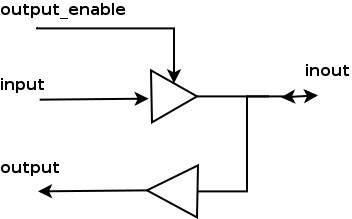
\includegraphics[width = 2 in]{LibFig/tristate}
\caption{TriState Buffer}
\label{tristate}
\end{center}
\end{figure}


The buffer has two
inputs,  an \te{input} of type \te{value\_type} and a Boolean
\te{output\_enable} which  determines the direction
of \te{inout}.  If 
\te{output\_enable} is True, the signal is 
coming in from  \te{input} and out through  \te{inout} and 
 \te{output}.  
 If  \te{output\_enable} is False, then a value can be driven in
 from  \te{inout}, and the \te{output} value will be the value of
  \te{inout}.  The behavior is described  in the tables below.  

\begin{center}
\begin{tabular}{|c|c||c|}
\hline
\multicolumn{3}{|c|}{output\_enable = 0}\\
\multicolumn{3}{|c|}{output = inout}\\
\hline
\multicolumn{2}{|c||}{Inputs}&\\
\cline{1-2}
input&inout&output\\
\hline
0&0&0\\
0&1&1\\
1&0&0\\
1&1&1\\
\hline
\end{tabular}
\end{center}

\begin{center}
\begin{tabular}{|c||c|c|}
\hline
\multicolumn{3}{|c|}{output\_enable = 1}\\
\multicolumn{3}{|c|}{output = in}\\
\multicolumn{3}{|c|}{inout = in}\\
\hline
&\multicolumn{2}{|c|}{Outputs}\\
\cline{2-3}
input&inout&output\\
\hline
0&0&0\\
1&1&1\\
\hline
\end{tabular}
\end{center}


This module is not supported in Bluesim.





{\bf Interfaces and Methods}

The \te{TriState} interface is composed of an \te{Inout} interface and
a \te{\_read} method.  The \te{\_read} method is similar to the
\te{\_read} method of a register in that to read the method you reference
  the  interface in an expression.

\index{TriState@\te{TriState} (interface)}
\begin{center}
\begin{tabular}{|p{.9 in}|p{1.4 in}|p{3.0 in}|}
\hline
\multicolumn{3}{|c|}{TriState Interface}\\
\hline
Name & Type & Description\\
\hline
\hline 
\te{io}  & \te{Inout\#(value\_type)} &\te{Inout} subinterface providing a value of  type \te{value\_type} \\
\hline
\te{\_read}&\te{value\_type}&Returns the value of \te{output} \\
\hline
\end{tabular}
\end{center}

\begin{libverbatim}
(* always_ready, always_enabled *)
interface TriState#(type value_type);
   interface Inout#(value_type)   io;
   method    value_type           _read;
endinterface: TriState
\end{libverbatim}


 

{\bf Modules and Functions}

The \te{TriState} package  provides a module constructor function,
\te{mkTriState}, which  provides the \te{TriState} interface.  The
interface includes an \te{Inout} subinterface and the value of \te{output}. 

\index{mkTriState@\te{mkTriState}}

\begin{center}
\begin{tabular}{|p{1 in}|p{4.5 in}|}
 \hline
&\\
\te{mkTriState}  & Creates a module which provides the
\te{TriState} interface.\\
\cline{2-2}
&\begin{libverbatim}
module mkTriState#(Bool output_enable, value_type input)
                  (TriState#(value_type))
   provisos(Bits#(value_type, size_value));
\end{libverbatim}
\\
\hline
\end{tabular}
\end{center}


{\bf Verilog Modules}

The \te{TriState} module is implemented by the Verilog module
\te{TriState.v} which can be found in the BSC {\V} library, \te{\$BLUESPECDIR/Verilog/}.


\subsubsection{ZBus}
\index{ZBus@\te{ZBus} (package)}

{\bf Package}

\begin{verbatim}
import ZBus :: * ;
\end{verbatim}


{\bf Description}

BSV provides the \te{ZBus} library to allow users to implement and use
tri-state buses. Since BSV does not support high-impedance or
undefined values internally, the library encapsulates the tri-state
bus implementation in a module that can only be accessed through
predefined interfaces which do not allow direct access to internal
signals (which could potentially have high-impedance or undefined
values).

The Verilog implementation of the tri-state module includes a number
of primitive submodules that are implemented using Verilog tri-state
wires. The BSV representation of the bus, however, only models the
values of the bus at the associated interfaces and thus the need to
represent high-impedance or undefined values in BSV is avoided.

A ZBus consists of a series of clients hanging off of a bus.  The
combination of the client and the bus is provided by the
\te{ZBusDualIFC} interface which consists of 2 subinterfaces, the client
and the bus.  The client subinterface is provided by the
\te{ZBusClientIFC} interface.    The bus subinterface is provided by the
\te{ZBusBusIFC} interface.  The user never needs to manipulate the bus
side, this is all done internally.  The user builds the bus out of
\te{ZBusDualIFC}s and then drives values onto the bus and reads values
from the bus using the \te{ZBusClientIFC}.


{\bf Interfaces and Methods}

There are three interfaces are defined in this package;
\te{ZBusDualIFC}, \te{ZBusClientIFC}, and \te{ZBusBusIFC}.

The
\te{ZBusDualIFC} interface provides two subinterfaces; a
\te{ZBusBusIFC} and a \te{ZBusClientIFC}.
For a given bus, one \te{ZBusDualIFC} interface is associated with
each bus client.


\index{ZBusDualIFC@\te{ZBusDualIFC} (interface)}
\begin{center}
\begin{tabular}{|p{.9 in}|p{1.4 in}|p{3.0 in}|}
\hline
\multicolumn{3}{|c|}{ZBusDualIFC}\\
\hline
Name & Type & Description\\
\hline
\hline 
\te{busIFC}  & \te{ZBusBusIFC\#()} &The subinterface providing the
bus side of the ZBus. \\
\hline
\te{clientIFC}&\te{ZBusClientIFC\#(t)}&The subinterface providing the
client side to the ZBus. \\
\hline
\end{tabular}
\end{center}

\begin{libverbatim}
interface ZBusDualIFC #(type value_type) ;
   interface ZBusBusIFC#(value_type)    busIFC;
   interface ZBusClientIFC#(value_type) clientIFC;
endinterface
\end{libverbatim}


The \te{ZBusClientIFC} allows a BSV module to connect to the tri-state
bus.   The \te{drive} method is used to drive a value onto the bus.  The \te{get()} and \te{fromBusValid()} methods  allow
each  bus client to access the 
current value on the bus. If the bus is in an invalid state (i.e. has
a high-impedance value or an undefined value because it is being
driven by more than one client simultaneously), then the
\te{get()} method will return \te{0} and the
\te{fromBusValid()} method will return \te{False}.  In all other
cases, the \te{fromBusValid()} method will return \te{True} and the
\te{get()} method will return the current value of the bus.


\begin{center}
\begin{tabular}{|p{.9 in}|p{.7 in}|p{1.5 in}|p{.4in}|p{1.5 in}|}
\hline
\multicolumn{5}{|c|}{ZBusClientIFC}\\
\hline
\multicolumn{3}{|c|}{Method}&\multicolumn{2}{|c|}{Argument}\\
\hline
Name & Type & Description& Name &\multicolumn{1}{|c|}{Description} \\
\hline
\hline 
\te{drive}  & Action &Drives a current value on to the bus
&\te{value}&The value being put on the bus, datatype of \te{value\_type}.\\
\hline
\te{get}&\te{value\_type}&Returns the current value on
the bus.&&\\
\hline
\te{fromBusValid}&\te{Bool}&Returns \te{False}
if the bus has a high-impedance value or is undefined.&&\\
\hline
\end{tabular}
\end{center}

\index{ZBusClientIFC@\te{ZBusClientIFC} (interface)}
\begin{libverbatim}
interface ZBusClientIFC #(type value_type) ;
   method Action      drive(value_type value);
   method value_type  get();
   method Bool        fromBusValid();
endinterface
\end{libverbatim}

The \te{ZBusBusIFC} interface
connects to the bus structure itself using tri-state values.  This
interface is never accessed directly by the user.

\index{ZBusBusIFC@\te{ZBusBusIFC} (interface)}

% \begin{center}
% \begin{tabular}{|p{.9 in}|p{.4 in}|p{1.7 in}|p{.4in}|p{1.7 in}|}
% \hline
% \multicolumn{5}{|c|}{ZBusBusIFC}\\
% \hline
% \multicolumn{3}{|c|}{Method}&\multicolumn{2}{|c|}{Argument}\\
% \hline
% Name & Type & Description& Name &\multicolumn{1}{|c|}{Description} \\
% \hline
% \hline 
% \te{fromBusSample}  & Action &Reads a current value from the bus
% &\te{value}&The value being read on the bus, datatype of \te{t}.\\
% \cline{4-5}
% &&&\te{isValid}&If \te{False}, a high-impedance value is driven onto the bus.\\
% \hline
% \te{toBusValue}&\te{ZBit\#(t)}& Drives  a  current value on to
% the bus.&&\\
% \hline
% \te{fromBusCtl}&\te{Bool}&Indicates whether the current value is a
% high-impedance value.  &&\\
% \hline
% \end{tabular}
% \end{center}

\begin{libverbatim}
interface ZBusBusIFC #(type value_type) ;
   method Action      fromBusSample(ZBit#(value_type) value, Bool isValid);
   method ZBit#(t)    toBusValue();
   method Bool        toBusCtl();
endinterface
\end{libverbatim}

 

{\bf Modules and Functions}

The library  provides a module constructor function,
\te{mkZBusBuffer}, which allows the user to create a module which
provides the \te{ZBusDualIFC} interface.  This module provides
  the functionality of a tri-state buffer.  

\index{mkZBusBuffer@\te{mkZBusBuffer} (function)}
\begin{center}
\begin{tabular}{|p{1 in}|p{4.5 in}|}
 \hline
&\\
\te{mkZBusBuffer}  & Creates a module which provides the
\te{ZBusDualIFC} interface.\\
\cline{2-2}
&\begin{libverbatim}
module mkZBusBuffer (ZBusDualIFC #(value_type)) 
   provisos (Eq#(value_type), Bits#(value_type, size_value));
\end{libverbatim}
\\
\hline
\end{tabular}
\end{center}


The \te{mkZBus} module
constructor function takes a list of \te{ZBusBusIFC}
interfaces as arguments and creates a module which ties them all
together  in a bus.

\index{mkZBus@\te{mkZBus} (function)}
\begin{center}
\begin{tabular}{|p{1 in}|p{4.5 in}|}
 \hline
&\\
\te{mkZBus}  & Ties a list of \te{ZBusBusIFC} interfaces
together in a bus.\\
\cline{2-2}
&\begin{libverbatim}
module mkZBus#(List#(ZBusBusIFC#(value_type)) ifc_list)(Empty)
   provisos (Eq#(value_type), Bits#(value_type, size_value));
\end{libverbatim}
\\
\hline
\end{tabular}
\end{center}




{\bf Examples - ZBus}

Creating a tri-state buffer for a 32 bit signal.  The interface is  named \te{buffer\_0}.
\begin{libverbatim}
   ZBusDualIFC#(Bit#(32)) buffer_0(); 
   mkZBusBuffer inst_buffer_0(buffer_0);
\end{libverbatim}

Drive a value of \te{12} onto the associated bus.
\begin{libverbatim}
   buffer_0.clientIFC.drive(12);
\end{libverbatim}


The following code fragment demonstrates the use of the module \te{mkZBus}.
\begin{libverbatim}
   ZBusDualIFC#(Bit#(32)) buffer_0();
   mkZBusBuffer inst_buffer_0(buffer_0);

   ZBusDualIFC#(Bit#(32)) buffer_1();
   mkZBusBuffer inst_buffer_1(buffer_1);

   ZBusDualIFC#(Bit#(32)) buffer_2();
   mkZBusBuffer inst_buffer_2(buffer_2);

   List#(ZBusIFC#(Bit#(32))) ifc_list;

   bus_ifc_list = cons(buffer_0.busIFC,
                        cons(buffer_1.busIFC,
                             cons(buffer_2.busIFC,
                                       nil)));

   Empty bus_ifc();
   mkZBus#(bus_ifc_list) inst_bus(bus_ifc);
\end{libverbatim}


\subsubsection{CRC}

\index{CRC@\te{CRC} (package)}

{\bf Package}

\begin{verbatim}
import CRC :: * ;
\end{verbatim}


{\bf Description}

CRC's are  designed to protect against common types of
errors on communication channels.  
The \te{CRC} package defines modules to calculate a check value for
each 8-bit block of data, which can then be verified to determine if
 data was transmitted and/or received correctly.   There are many commonly used and
standardized  CRC algorithms. 
The \te{CRC} package provides both a generalized CRC module as well as
module implementations for the CRC-CCITT, CRC-16-ANSI, and
CRC-32 (IEEE 802.3) standards. The size of the CRC polynomial
 is polymorphic and  the data
 size is a byte (\te{Bit\#(8)}),  which is relevant for many
 applications.  The generalized module uses five 
arguments to define the CRC algorithm: the CRC polynomial,   the initial
CRC value, a fixed bit pattern to Xor with the remainder, a boolean indicating whether to reverse the data
bit order and a boolean indicating whether to reverse the result bit
order.  By specifying these 
arguments, you can implement many CRC algorithms.  This package 
provides modules for three specific algorithms by defining the
arguments for those algorithms.


{\bf Interfaces and Methods}

The CRC modules provide the \te{CRC} interface.  The \te{add} method
is used to calculate the check value on the \te{data} argument.  In
this package, the argument is always a \te{Bit\#(8)}.  
 

\begin{center}
\begin{tabular}{|p{.5in}|p{1.5in}|p{1.2 in}|p{.9in}|p{1 in}|}
\hline
\multicolumn{5}{|c|}{\te{CRC} Interface}\\
\hline
\multicolumn{3}{|c|}{Method}&\multicolumn{2}{|c|}{Arguments}\\
\hline
Name & Type & Description& Name &\multicolumn{1}{|c|}{Description} \\
\hline
\hline 
\te{add}&\te{Action}&Update the CRC  &\te{Bit\#(8) data}&8-bit data block\\
\hline
\te{clear}&\te{Action} &\multicolumn{3}{|l|}{Reset to the initial value}\\
\hline
\te{result}&\te{Bit\#(n)}&\multicolumn{3}{|l|}{Returns the current value of the check value}\\
\hline
\te{complete}&\te{ActionValue(Bit\#(n))}&\multicolumn{3}{|l|}{Return the result and reset}\\
\hline
\end{tabular}
\end{center}
 

\begin{libverbatim}
interface CRC#(numeric type n);
   method    Action   add(Bit#(8) data);
   method    Action   clear();
   method    Bit#(n)  result();
   method    ActionValue#(Bit#(n)) complete();
endinterface
\end{libverbatim}

{\bf Modules}


\index{mkCRC@\te{mkCRC}(module)}

The implementation of the generalized CRC module takes the following
five arguments:
\begin{itemize}
\item \te{Bit\#(n)} polynomial:  the crc operation polynomial,  for example
$x^{16} + x^{12} + x^{5}+ 1$ is written as $`h1021$

\item \te{Bit\#(n)} initval: the initial CRC value

\item \te{Bit\#(n)} finalXor: the result is xor'd with this value if
desired
\item \te{Bool} reflectData: if True, reverse the data bit order

\item \te{Bool} reflectRemainder: if True, reverse the result bit order
\end{itemize}



\begin{center}
\begin{tabular}{|p{1 in}|p{4.8 in}|}
\hline
&\\
\te{mkCRC}&The generalized CRC module. The provisos enforce the
requirement that polynomial and initial value  must be at least 8 bits. \\
\cline{2-2}
&\begin{libverbatim}
module mkCRC#(  Bit#(n) polynomial      
	      , Bit#(n) initval         
	      , Bit#(n) finalXor       
	      , Bool    reflectData    
	      , Bool    reflectRemainder 
	      )(CRC#(n))
   provisos(  Add#(8, n8, n) );
\end{libverbatim}
\\
\hline
\end{tabular}
\end{center}


\begin{center}
\begin{tabular}{|l|l|l|l|l|l|}
\hline
\multicolumn{6}{|c|}{CRC Arguments for Common Standards}\\
\hline
Name&polynomial&initval&finalXor&reflectData&reflectRemainder\\
\hline
\hline
CRC-CCITT&\te{'h1021}&\te{'hFFFF }&
\te{'h0000}&\te{False}&\te{False}\\
\hline
 CRC-16-ANSI&\te{'h8005}&\te{'h0000 }&\te{'h0000}&\te{True}&\te{True}\\
\hline
CRC-32 (IEEE 802.3)&
\te{'h04C11DB7}&\te{'hFFFFFFFF}&\te{'hFFFFFFFF}&\te{True}&\te{True}\\
\hline

\end{tabular}
\end{center}


\index{mkCRC\_CCITT@\te{mkCRC\_CCIT}(module)}


\begin{center}
\begin{tabular}{|p{1 in}|p{4.8 in}|}
\hline
&\\
\te{mkCRC\_CCIT}& Implements the 16-bit CRC-CCITT standard.   \\
&($x^{16} + x^{15} + x^{2} + 1$).   \\
\cline{2-2}
&\begin{libverbatim}
module mkCRC_CCITT(CRC#(16));
\end{libverbatim}
\\
\hline
\end{tabular}
\end{center}



\index{mkCRC16@\te{mkCRC16}(module)}

\begin{center}
\begin{tabular}{|p{1 in}|p{4.8 in}|}
\hline
&\\
\te{mkCRC16}& Implementation of the  16-bit CRC-16-ANSI standard. \\
& ($x^{16} + x^{15} + x^{2} + 1$).\\
\cline{2-2}
&\begin{libverbatim}
module mkCRC16(CRC#(16));
\end{libverbatim}
\\
\hline
\end{tabular}
\end{center}


\index{mkCRC32@\te{mkCRC32}(module)}

\begin{center}
\begin{tabular}{|p{1 in}|p{4.8 in}|}
\hline
&\\
\te{mkCRC32}& Implementation of the 32-bit CRC-32 (IEEE 802.3)
standard. \\
&($x^{32} + x^{26} + x^{23} + x^{22} + x^{16} + x^{12} + x^{11} + x^{10} + x^{8} + x^{7} + x^{5} + x^{4} + x^{2} + x^{1} + 1$)\\
\cline{2-2}
&\begin{libverbatim}
module mkCRC32(CRC#(32));
\end{libverbatim}
\\
\hline
\end{tabular}
\end{center}

\index{reflect@\te{reflect}(CRC function)}
\begin{center}
\begin{tabular}{|p{1 in}|p{4.8 in}|}
\hline
&\\
\te{reflect}&The \te{reflect} function reverses the data bits if the
value of \te{reflectData} is \te{True}. \\
\cline{2-2}
&\begin{libverbatim}
function Bit#(a) reflect(Bool doIt, Bit#(a) data);
   return (doIt) ? reverseBits(data) : data;
endfunction
\end{libverbatim}
\\
\hline
\end{tabular}
\end{center}




\subsubsection{OVLAssertions}

\index{OVLAssertions (package)}

{\bf Package}

\begin{verbatim}
import OVLAssertions :: * ;
\end{verbatim}



{\bf Description}

The OVLAssertions package provides the {\BSV} interfaces and wrapper
modules necessary to allow {\BSV} designs to include assertion
checkers from the Open Verification Library (OVL).  The OVL includes a
set of assertion checkers that verify specific properties of a design.
For more details on the complete OVL, refer to the Accellera Standard
OVL Library Reference Manual (\te{http://www.accellera.org}).



{\bf Interfaces and Methods}


The following interfaces are defined for use with the assertion
modules.  Each interface has one or more \te{Action} methods.  Each
method takes a single argument which is either a \te{Bool} or
polymorphic.   

% \begin{center}
% \begin{tabular}{|p{1.8 in}|p{3.6 in}|}
% \hline
% Interface&Description\\
% \hline
% \te{AssertTest\_IFC}&Used for assertions that check a test
% expression on every clock cycle.\\
% \hline
% \te{AssertSampleTest\_IFC}&Used for assertions that check a test
% expression on every clock cycle only when sample is asserted.\\
% \hline
% \te{AssertStartTest\_IFC}& Used for assersions that check a test expression only subsequent to a start\_event.\\
% \hline
% \te{AssertStartStopTest\_IFC}& Used to check a test expression between
% a start\_event and an end\_event.\\
% \hline
% \te{AssertTransitionTest\_IFC}&Used to check a test expression that
% has a specified start state and next state, i.e. a
% transition.\\
% \hline
% \te{AssertQuiescentTest\_IFC}&Used to check that a test expression
% equals a check expression when a state is
% asserted.\\
% \hline
% \te{AssertFIFOTest\_IFC}&Used with a FIFO structures.\\
% \hline
% \end{tabular}
% \end{center}

\paragraph{AssertTest\_IFC}
%\index{OVL Assertions!AssertTest\_IFC@\te{AssertTest\_IFC} (interface)}
\index{AssertTest\_IFC@\te{AssertTest\_IFC} (interface)}

Used for assertions that check a test expression on every clock cycle.
\begin{center}
\begin{tabular}{|p{.6in}|p{.5 in}|p{.8 in}|p{.7 in}|p{2.5 in}|}
\hline
\multicolumn{5}{|c|}{\te{AssertTest\_IFC}}\\
 \hline
\multicolumn{2}{|c|}{Method}&\multicolumn{3}{|c|}{Argument}\\
\hline
Name&Type&Name&Type&Description\\
\hline
\hline
\te{test}&\te{Action}&\te{test\_value}&\te{a\_type}&Expression to be checked.\\
\hline
\end{tabular}
\end{center}

\begin{libverbatim}
interface AssertTest_IFC #(type a_type);
   method Action test(a_type test_value);
endinterface
\end{libverbatim}

\paragraph{AssertSampleTest\_IFC}
\index{AssertSampleTest\_IFC@\te{AssertSampleTest\_IFC} (interface)}
%\index{OVL Assertions!AssertSampleTest\_IFC@\te{AssertSampleTest\_IFC} (interface)}

Used for assertions that check a test expression on every clock cycle
only if the sample, indicated by the boolean value \te{sample\_test}
is asserted.
\begin{center}
\begin{tabular}{|p{.6in}|p{.5 in}|p{.8 in}|p{.7 in}|p{2.5 in}|}
\hline
\multicolumn{5}{|c|}{\te{AssertSampleTest\_IFC}}\\
 \hline
\multicolumn{2}{|c|}{Method}&\multicolumn{3}{|c|}{Argument}\\
\hline
Name&Type&Name&Type&Description\\
\hline
\hline
\te{sample}&\te{Action}&\te{sample\_test}&\te{Bool}&Assertion
only checked if \te{sample\_test} is asserted.\\
\hline
\te{test}&\te{Action}&\te{test\_value}&\te{a\_type}&Expression to be checked.\\
\hline
\end{tabular}
\end{center}

\begin{libverbatim}
interface AssertSampleTest_IFC #(type a_type);
   method Action sample(Bool sample_test);
   method Action test(a_type test_value);
endinterface
\end{libverbatim}

\paragraph{AssertStartTest\_IFC}
\index{AssertStartTest\_IFC@\te{AssertStartTest\_IFC} (interface)}
%\index{OVL Assertions!AssertStartTest\_IFC@\te{AssertStartTest\_IFC} (interface)}

Used for assertions that check a test expression only subsequent to a
start\_event, specified by the Boolean value \te{start\_test}.
\begin{center}
\begin{tabular}{|p{.6in}|p{.5 in}|p{.8 in}|p{.7 in}|p{2.5 in}|}
\hline
\multicolumn{5}{|c|}{\te{AssertStartTest\_IFC}}\\
 \hline
\multicolumn{2}{|c|}{Method}&\multicolumn{3}{|c|}{Argument}\\
\hline
Name&Type&Name&Type&Description\\
\hline
\hline
\te{start}&\te{Action}&\te{start\_test}&\te{Bool}&Assertion
only checked after start is asserted.\\
\hline
\te{test}&\te{Action}&\te{test\_value}&\te{a\_type}&Expression to be checked.\\
\hline
\end{tabular}
\end{center}

\begin{libverbatim}
interface AssertStartTest_IFC #(type a_type);
   method Action start(Bool start_test);
   method Action test(a_type test_value);
endinterface
\end{libverbatim}

\paragraph{AssertStartStopTest\_IFC}
\index{AssertStartStopTest\_IFC@\te{AssertStartStopTest\_IFC}
(interface)}
%\index{OVL Assertions!AssertStartStopTest\_IFC@\te{AssertStartStopTest\_IFC} (interface)}

Used to check a test expression between a start\_event and a
stop\_event.
\begin{center}
\begin{tabular}{|p{.6in}|p{.5 in}|p{.8 in}|p{.7 in}|p{2.5 in}|}
\hline
\multicolumn{5}{|c|}{\te{AssertStartStopTest\_IFC}}\\
 \hline
\multicolumn{2}{|c|}{Method}&\multicolumn{3}{|c|}{Argument}\\
\hline
Name&Type&Name&Type&Description\\
\hline
\hline
\te{start}&\te{Action}&\te{start\_test}&\te{Bool}&Assertion
only checked after start is asserted.\\
\hline
\te{stop}&\te{Action}&\te{stop\_test}&\te{Bool}&Assertion
only checked until the stop is asserted.\\
\hline
\te{test}&\te{Action}&\te{test\_value}&\te{a\_type}&Expression to be checked.\\
\hline
\end{tabular}
\end{center}

\begin{libverbatim}
interface AssertStartStopTest_IFC #(type a_type);
   method Action start(Bool start_test);
   method Action stop(Bool stop_test);
   method Action test(a_type test_value);
endinterface
\end{libverbatim}

\paragraph{AssertTransitionTest\_IFC}
\index{AssertTransitionTest\_IFC@\te{AssertTransitionTest\_IFC} (interface)}
%\index{OVL Assertions!AssertTransitionTest\_IFC@\te{AssertTransitionTest\_IFC}
%(interface)}

Used to check a test expression that
has a specified start state and next state, i.e. a
transition.
\begin{center}
\begin{tabular}{|p{.6in}|p{.5 in}|p{.8 in}|p{.7 in}|p{2.5 in}|}
\hline
\multicolumn{5}{|c|}{\te{AssertTransitionTest\_IFC}}\\
 \hline
\multicolumn{2}{|c|}{Method}&\multicolumn{3}{|c|}{Argument}\\
\hline
Name&Type&Name&Type&Description\\
\hline
\hline
\te{test}&\te{Action}&\te{test\_value}&\te{a\_type}&Expression that
should transition to the \te{next\_value}.\\
\hline
\te{start}&\te{Action}&\te{start\_test}&\te{a\_type}&Expression that
indicates the start state for the assertion check.  If the value of
\te{start\_test} equals the value of \te{test\_value}, the check is performed.\\
\hline
\te{next}&\te{Action}&\te{next\_value}&\te{a\_type}&Expression that
indicates  the only valid next state for the assertion check.\\
\hline
\end{tabular}
\end{center}

\begin{libverbatim}
interface AssertTransitionTest_IFC #(type a_type);
   method Action test(a_type test_value);
   method Action start(a_type start_value);
   method Action next(a_type next_value);
endinterface
\end{libverbatim}

\paragraph{AssertQuiescentTest\_IFC}
\index{AssertQuiescentTest\_IFC@\te{AssertQuiescentTest\_IFC} (interface)}
%\index{OVL Assertions!AssertQuiescentTest\_IFC@\te{AssertQuiescentTest\_IFC} (interface)}

Used to check that a test expression is equivalent to the specified expression
when the sample state is asserted.
\begin{center}
\begin{tabular}{|p{.6in}|p{.5 in}|p{.8 in}|p{.7 in}|p{2.5 in}|}
\hline
\multicolumn{5}{|c|}{\te{AssertQuiescentTest\_IFC}}\\
 \hline
\multicolumn{2}{|c|}{Method}&\multicolumn{3}{|c|}{Argument}\\
\hline
Name&Type&Name&Type&Description\\
\hline
\hline
\te{sample}&\te{Action}&\te{sampe\_test}&\te{Bool}&Expression which
initiates  the
quiescent assertion check when it transistions to true.\\
\hline
\te{state}&\te{Action}&\te{state\_value}&\te{a\_type}&Expression that
should have the same value as \te{check\_value}\\
\hline
\te{check}&\te{Action}&\te{check\_value}&\te{a\_type}&Expression
\te{state\_value} is compared to.\\
\hline
\end{tabular}
\end{center}

\begin{libverbatim}
interface AssertQuiescentTest_IFC #(type a_type);
   method Action sample(Bool sample_test);
   method Action state(a_type state_value);
   method Action check(a_type check_value);
endinterface
\end{libverbatim}

\paragraph{AssertFifoTest\_IFC}
\index{AssertFifoTest\_IFC@\te{AssertFifoTest\_IFC} (interface)}
%\index{OVL Assertions!AssertFifoTest\_IFC@\te{AssertFifoTest\_IFC} (interface)}

Used with assertions checking  a FIFO structure.
\begin{center}
\begin{tabular}{|p{.6in}|p{.5 in}|p{.8 in}|p{.7 in}|p{2.5 in}|}
\hline
\multicolumn{5}{|c|}{\te{AssertFifoTest\_IFC}}\\
 \hline
\multicolumn{2}{|c|}{Method}&\multicolumn{3}{|c|}{Argument}\\
\hline
Name&Type&Name&Type&Description\\
\hline
\hline
\te{push}&\te{Action}&\te{push\_value}&\te{a\_type}&Expression which
indicates the number of push operations that will occur during the
current cycle.\\
\hline
\te{pop}&\te{Action}&\te{pop\_value}&\te{a\_type}&Expression which
indicates the number of pop operations that will occur during the
current cycle.\\
\hline
\end{tabular}
\end{center}

\begin{libverbatim}
interface AssertFifoTest_IFC #(type a_type, type b_type);
   method Action push(a_type push_value);
   method Action pop(b_type pop_value);
endinterface
\end{libverbatim}

{\bf Datatypes}

The parameters
\te{severity\_level}, \te{property\_type}, \te{msg}, and
\te{coverage\_level} are common to all assertion checkers.  

\begin{center}
\begin{tabular}{|p {2.0 in}|p{2.5 in}|}
\hline
\multicolumn{2}{|c|}{Common Parameters for all Assertion Checkers}\\
\hline
Parameter&Valid Values\\
&* indicates default value\\
\hline
\hline
\te{severity\_level}&\te{OVL\_FATAL}\\
&*\te{OVL\_ERROR}\\
&\te{OVL\_WARNING}\\
&\te{OVL\_Info}\\
\hline
\te{property\_type}&*\te{OVL\_ASSERT}\\
&\te{OVL\_ASSUME}\\
&\te{OVL\_IGNORE}\\
\hline
\te{msg}&*\te{VIOLATION}\\
\hline
\te{coverage\_level}&\te{OVL\_COVER\_NONE}\\
&*\te{OVL\_COVER\_ALL}\\
&\te{OVL\_COVER\_SANITY}\\
&\te{OVL\_COVER\_BASIC}\\
&\te{OVL\_COVER\_CORNER}\\
&\te{OVL\_COVER\_STATISTIC}\\
\hline
\end{tabular}
\end{center}

Each assertion checker may also use some subset of the following parameters.

\begin{center}
\begin{tabular}{|p {2.0 in}|p{2.5 in}|}
\hline
\multicolumn{2}{|c|}{Other Parameters for Assertion Checkers}\\
\hline
Parameter&Valid Values\\
\hline
\hline
\te{action\_on\_new\_start}&\te{OVL\_IGNORE\_NEW\_START}\\
&\te{OVL\_RESET\_ON\_NEW\_START}\\
&\te{OVL\_ERROR\_ON\_NEW\_START}\\
\hline
\te{edge\_type}&\te{OVL\_NOEDGE}\\
&\te{OVL\_POSEDGE}\\
&\te{OVL\_NEGEDGE}\\
&\te{OVL\_ANYEDGE}\\
\hline
\te{necessary\_condition}&\te{OVL\_TRIGGER\_ON\_MOST\_PIPE}\\
&\te{OVL\_TRIGGER\_ON\_FIRST\_PIPE}\\
&\te{OVL\_TRIGGER\_ON\_FIRST\_NOPIPE}\\
\hline
\te{inactive}&\te{OVL\_ALL\_ZEROS}\\
&\te{OVL\_ALL\_ONES}\\
&\te{OVL\_ONE\_COLD}\\
\hline
\end{tabular}
\end{center}
\begin{center}
\begin{tabular}{|p {2.0 in}|p{2.5 in}|}
\hline
\multicolumn{2}{|c|}{Other Parameters for Assertion Checkers}\\
\hline
Parameter&Valid Values\\
\hline
\hline
\te{num\_cks}&\te{Int\#(32)}\\
\hline
\te{min\_cks}&\te{Int\#(32)}\\
\hline
\te{max\_cks}&\te{Int\#(32)}\\
\hline
\te{min\_ack\_cycle}&\te{Int\#(32)}\\
\hline
\te{max\_ack\_cycle}&\te{Int\#(32)}\\
\hline
\te{max\_ack\_length}&\te{Int\#(32)}\\
\hline
\te{req\_drop}&\te{Int\#(32)}\\
\hline
\te{deassert\_count}&\te{Int\#(32)}\\
\hline
\te{depth}&\te{Int\#(32)}\\
\hline
\te{value}&\te{a\_type}\\
\hline
\te{min}&\te{a\_type}\\
\hline
\te{max}&\te{a\_type}\\
\hline
\te{check\_overlapping}&\te{Bool}\\
\hline
\te{check\_missing\_start}&\te{Bool}\\
\hline
\te{simultaneous\_push\_pop}&\te{Bool}\\
\hline	
\end{tabular}
\end{center}

{\bf Setting Assertion Parameters}

Each assertion checker module has a set of associated parameter values
that can be customized for each module instantiation. The values for
these parameters are passed to each checker module in the form of a
single struct argument of type \te{OVLDefaults\#(a)}  A typical use scenario
is illustrated below: 

\begin{verbatim}
let defaults = mkOVLDefaults;

defaults.min_clks = 2;
defaults.max_clks = 3;

AssertTest_IFC#(Bool) assertWid <- bsv_assert_width(defaults);
\end{verbatim}

The defaults struct (created by \te{mkOVLDefaults}) includes one field for
each possible parameter. Initially each field includes the associated
default value. By editing fields of the struct,  individual parameter
values can be modified as needed to be non-default values.  The
modified \te{defaults} struct is then  provided as a module argument during
instantiation. 


% {\bf Parameters}

% Every assertion checker has a defined set of parameters, each of which
% must have a value.   Use the module  \te{mkOVLDefaults}
% to set default values for all the parameters.  Then set individual
% parameters (\te{default.}{\em field name}) as needed to the non-default values.
% \begin{libverbatim}
%    \\ set the defaults
%    let defaults = mkOVLDefaults;
   
%    \\ set the specific parameters to non-default values
%    defaults.min_cks = 2; //min_cks : 2
%    defaults.max_cks = 3; //max_cks : 3
% \end{libverbatim}


{\bf Modules}

Each module in this package corresponds to an assertion checker from the Open
Verification Library (OVL).  The {\BSV} name for each module is the same as the OVL name
with \te{bsv\_} appended to the beginning of the  name.


%===============================================
\index{bsv\_assert\_always@\te{bsv\_assert\_always} (module)}
\index[function]{OVLAssertions!bsv\_assert\_always}
%\index{OVL Assertions!bsv\_assert\_always@\te{bsv\_assert\_always} (module)}
\begin{center}
\begin{tabular}{|p{1.2 in}|p{4.3 in}|}
\hline
Module&\te{bsv\_assert\_always}\\
\hline
Description&Concurrent assertion that the value of the
expression is always \te{True}.\\
\hline
Interface Used&\te{AssertTest\_IFC}\\
\hline
Parameters&common assertion parameters\\
\hline
Module Declaration&\begin{libverbatim}
module bsv_assert_always#(OVLDefaults#(Bool) defaults) 
               (AssertTest_IFC#(Bool));
\end{libverbatim}
\\
\hline
\end{tabular}
\end{center}

%===============================================
\index{bsv\_assert\_always\_on\_edge@\te{bsv\_assert\_always\_on\_edge}
(module)}
\index[function]{OVLAssertions!bsv\_assert\_always\_on\_edge}
%\index{OVL Assertions!bsv\_assert\_always\_on\_edge@\te{bsv\_assert\_always\_on\_edge} (module)}
\begin{center}
\begin{tabular}{|p{1.2 in}|p{4.3 in}|}
\hline
Module&\te{bsv\_assert\_always\_on\_edge}\\
\hline
Description&Checks that the test expression
evaluates \te{True} whenever the sample method is asserted. \\
\hline
Interface Used&\te{AssertSampleTest\_IFC}\\
\hline
Parameters&common assertion parameters\\
&\te{edge\_type} (default value = \te{OVL\_NOEDGE})\\
\hline
Module Declaration&\begin{libverbatim}
module bsv_assert_always_on_edge#(OVLDefaults#(Bool) 
               defaults)(AssertSampleTest_IFC#(Bool));
\end{libverbatim}
\\
\hline
\end{tabular}
\end{center}
%===============================================
\index{bsv\_assert\_change@\te{bsv\_assert\_change} (module)}
\index[function]{OVLAssertions!bsv\_assert\_change}
%\index{OVL Assertions!bsv\_assert\_change@\te{bsv\_assert\_change} (module)}
\begin{center}
\begin{tabular}{|p{1.2 in}|p{4.3 in}|}
\hline
Module&\te{bsv\_assert\_change}\\
\hline
Description&Checks that once the start method is
asserted, the expression will change value within \te{num\_cks} cycles. \\
\hline
Interface Used&\te{AssertStartTest\_IFC}\\
\hline
Parameters&common assertion parameters\\
&\te{action\_on\_new\_start} (default value = \te{OVL\_IGNORE\_NEW\_START})\\
&\te{num\_cks} (default value = 1) \\
\hline
Module Declaration&\begin{libverbatim}
module bsv_assert_change#(OVLDefaults#(a_type) defaults) 
               (AssertStartTest_IFC#(a_type))
    provisos (Bits#(a_type, sizea), 
              Bounded#(a_type), Eq#(a_type));
\end{libverbatim}
\\
\hline
\end{tabular}
\end{center}
%===============================================
%===============================================
\index{bsv\_assert\_cycle\_sequence@\te{bsv\_assert\_cycle\_sequence} (module)}
\index[function]{OVLAssertions!bsv\_assert\_cycle\_sequence}
%\index{OVL Assertions!bsv\_assert\_cycle\_sequence@\te{bsv\_assert\_cycle\_sequence} (module)}
\begin{center}
\begin{tabular}{|p{1.2 in}|p{4.3 in}|}
\hline
Module&\te{bsv\_assert\_cycle\_sequence}\\
\hline
Description&Ensures that if a specified necessary condition occurs,it is followed by a
specified sequence of events. \\
\hline
Interface Used&\te{AssertTest\_IFC}\\
\hline
Parameters&common assertion parameters\\
&\te{necessary\_condition} (default value = \te{OVL\_TRIGGER\_ON\_MOST\_PIPE})\\
%% &\te{num\_cks} (default value = 2)\\
\hline
Module Declaration&\begin{libverbatim}
module bsv_assert_cycle_sequence#(OVLDefaults#(a_type) 
               defaults)(AssertTest_IFC#(a_type))  
     provisos (Bits#(a_type, sizea), 
               Bounded#(a_type), Eq#(a_type));
\end{libverbatim}
\\
\hline
\end{tabular}
\end{center}
%=================================================
\index{bsv\_assert\_decrement@\te{bsv\_assert\_decrement} (module)}
\index[function]{OVLAssertions!bsv\_assert\_decrement}
%\index{OVL Assertions!bsv\_assert\_decrement@\te{bsv\_assert\_decrement} (module)}
\begin{center}
\begin{tabular}{|p{1.2 in}|p{4.3 in}|}
\hline
Module&\te{bsv\_assert\_decrement}\\
\hline
Description&Ensures that the expression decrements only by the value
specifiedR. \\
\hline
Interface Used&\te{AssertTest\_IFC}\\
\hline
Parameters&common assertion parameters\\
&\te{value} (default value = 1)\\
\hline
Module Declaration&\begin{libverbatim}
module bsv_assert_decrement#(OVLDefaults#(a_type) defaults)
               (AssertTest_IFC#(a_type))
    provisos (Bits#(a_type, sizea), Literal#(a_type), 
              Bounded#(a_type), Eq#(a_type));
\end{libverbatim}
\\
\hline
\end{tabular}
\end{center}
%==============================================
\index{bsv\_assert\_delta@\te{bsv\_assert\_delta} (module)}
\index[function]{OVLAssertions!bsv\_assert\_delta}
%\index{OVL Assertions!bsv\_assert\_delta@\te{bsv\_assert\_delta} (module)}
\begin{center}
\begin{tabular}{|p{1.2 in}|p{4.3 in}|}
\hline
Module&\te{bsv\_assert\_delta}\\
\hline
Description& Ensures that the expression always changes by a value
within the range specified by \te{min} and \te{max}. \\
\hline
Interface Used&\te{AssertTest\_IFC}\\
\hline
Parameters&common assertion parameters\\
&\te{min} (default value = 1)\\
&\te{max} (default value = 1)\\
\hline
Module Declaration&\begin{libverbatim}
module bsv_assert_delta#(OVLDefaults#(a_type) defaults)
               (AssertTest_IFC#(a_type))
    provisos (Bits#(a_type, sizea), Literal#(a_type), 
              Bounded#(a_type), Eq#(a_type));
\end{libverbatim}
\\
\hline
\end{tabular}
\end{center}
%===============================================
\index{bsv\_assert\_even\_parity@\te{bsv\_assert\_even\_parity} (module)}
\index[function]{OVLAssertions!bsv\_assert\_even\_parity}
%\index{OVL Assertions!bsv\_assert\_even\_parity@\te{bsv\_assert\_even\_parity} (module)}
\begin{center}
\begin{tabular}{|p{1.2 in}|p{4.3 in}|}
\hline
Module&\te{bsv\_assert\_even\_parity}\\
\hline
Description&Ensures that value of a specified expression has even
parity, that is an even number of bits in the expression
are active high.\\
\hline
Interface Used&\te{AssertTest\_IFC}\\
\hline
Parameters&common assertion parameters\\
\hline
Module Declaration&\begin{libverbatim}
module bsv_assert_even_parity#(OVLDefaults#(a_type) 
               defaults) (AssertTest_IFC#(a_type))
    provisos (Bits#(a_type, sizea), 
              Bounded#(a_type), Eq#(a_type));
\end{libverbatim}
\\
\hline
\end{tabular}
\end{center}

%===============================================
\index{bsv\_assert\_fifo\_index@\te{bsv\_assert\_fifo\_index}
(module)}
\index[function]{OVLAssertions!bsv\_assert\_fifo\_index}
%\index{OVL Assertions!bsv\_assert\_fifo\_index@\te{bsv\_assert\_fifo\_index} (module)}
\begin{center}
\begin{tabular}{|p{1.2 in}|p{4.3 in}|}
\hline
Module&\te{bsv\_assert\_fifo\_index}\\
\hline
Description&Ensures that a FIFO-type structure never overflows or underflows. 
 This checker can be configured to support multiple pushes 
        (FIFO writes) and pops (FIFO reads) during the same clock cycle.  \\
\hline
Interface Used&\te{AssertFifoTest\_IFC}\\
\hline
Parameters&common assertion parameters\\
&\te{depth} (default value = 1) \\
&\te{simultaneous\_push\_pop} (default value = \te{True})\\
\hline
Module Declaration&\begin{libverbatim}
module bsv_assert_fifo_index#(OVLDefaults#(Bit#(0)) 
            defaults)(AssertFifoTest_IFC#(a_type, b_type))
    provisos (Bits#(a_type, sizea), Bits#(b_type, sizeb));
\end{libverbatim}
\\
\hline
\end{tabular}
\end{center}
%=================================================
   
%===============================================
\index{bsv\_assert\_frame@\te{bsv\_assert\_frame} (module)}
\index[function]{OVLAssertions!bsv\_assert\_frame}
%\index{OVL Assertions!bsv\_assert\_frame@\te{bsv\_assert\_frame} (module)}
\begin{center}
\begin{tabular}{|p{1.2 in}|p{4.3 in}|}
\hline
Module&\te{bsv\_assert\_frame}\\
\hline
Description&Checks that once the start method is asserted, the test 
 expression evaluates true not before \te{min\_cks} clock cycles 
  and not after \te{max\_cks} clock cycles.   \\
\hline
Interface Used&\te{AssertStartTest\_IFC}\\
\hline
Parameters&common assertion parameters\\
&\te{action\_on\_new\_start} (default value = \te{OVL\_IGNORE\_NEW\_START})\\
&\te{min\_cks} (default value = 1) \\
&\te{max\_cks} (default value = 1) \\
\hline
Module Declaration&\begin{libverbatim}
module bsv_assert_frame#(OVLDefaults#(Bool) defaults) 
               (AssertStartTest_IFC#(Bool));
\end{libverbatim}
\\
\hline
\end{tabular}
\end{center}
%===============================================
\index{bsv\_assert\_handshake@\te{bsv\_assert\_handshake} (module)}
\index[function]{OVLAssertions!bsv\_assert\_handshake}
%\index{OVL Assertions!bsv\_assert\_handshake@\te{bsv\_assert\_handshake} (module)}
\begin{center}
\begin{tabular}{|p{1.2 in}|p{4.3 in}|}
\hline
Module&\te{bsv\_assert\_handshake}\\
\hline
Description&Ensures that the specified request and acknowledge signals
follow a specified handshake protocol.\\
\hline
Interface Used&\te{AssertStartTest\_IFC}\\
\hline
Parameters&common assertion parameters\\
&\te{action\_on\_new\_start}  (default value = \te{OVL\_IGNORE\_NEW\_START})\\
&\te{min\_ack\_cycle}  (default value = 1)\\
&\te{max\_ack\_cycle}  (default value = 1)\\
\hline
Module Declaration&\begin{libverbatim}
module bsv_assert_handshake#(OVLDefaults#(Bool) defaults) 
               (AssertStartTest_IFC#(Bool));
\end{libverbatim}
\\
\hline
\end{tabular}
\end{center}
%===============================================
\index{bsv\_assert\_implication@\te{bsv\_assert\_implication}
(module)}
\index[function]{OVLAssertions!bsv\_assert\_implication}
%\index{OVL Assertions!bsv\_assert\_implication@\te{bsv\_assert\_implication} (module)}
\begin{center}
\begin{tabular}{|p{1.2 in}|p{4.3 in}|}
\hline
Module&\te{bsv\_assert\_implication}\\
\hline
Description&Ensures that a specified consequent expression is
\te{True} if the specified antecedent expression is \te{True}. \\
\hline
Interface Used&\te{AssertStartTest\_IFC}\\
\hline
Parameters&common assertion parameters\\

\hline
Module Declaration&\begin{libverbatim}
module bsv_assert_implication#(OVLDefaults#(Bool) defaults) 
               (AssertStartTest_IFC#(Bool));
\end{libverbatim}
\\
\hline
\end{tabular}
\end{center}
 

%===============================================
\index{bsv\_assert\_increment@\te{bsv\_assert\_increment} (module)}
\index[function]{OVLAssertions!bsv\_assert\_increment}
%\index{OVL Assertions!bsv\_assert\_increment@\te{bsv\_assert\_increment} (module)}
\begin{center}
\begin{tabular}{|p{1.2 in}|p{4.3 in}|}
\hline
Module&\te{bsv\_assert\_increment}\\
\hline
Description&ensure that the test expression always increases by the
value of specified by \te{value}. \\
\hline
Interface Used&\te{AssertTest\_IFC}\\
\hline
Parameters&common assertion parameters\\
&\te{value} (default value = 1)\\
\hline
Module Declaration&\begin{libverbatim}
module bsv_assert_increment#(OVLDefaults#(a_type) defaults) 
               (AssertTest_IFC#(a_type))
    provisos (Bits#(a_type, sizea), Literal#(a_type), 
              Bounded#(a_type), Eq#(a_type));
\end{libverbatim}
\\
\hline
\end{tabular}
\end{center}
%=================================================


   
%===============================================
\index{bsv\_assert\_never@\te{bsv\_assert\_never} (module)}
\index[function]{OVLAssertions!bsv\_assert\_never}
%\index{OVL Assertions!bsv\_assert\_never@\te{bsv\_assert\_never} (module)}
\begin{center}
\begin{tabular}{|p{1.2 in}|p{4.3 in}|}
\hline
Module&\te{bsv\_assert\_never}\\
\hline
Description&Ensures that the value of a specified expression is never \te{True}. \\
\hline
Interface Used&\te{AssertTest\_IFC}\\
\hline
Parameters&common assertion parameters\\

\hline
Module Declaration&\begin{libverbatim}
module bsv_assert_never#(OVLDefaults#(Bool) defaults) 
               (AssertTest_IFC#(Bool));
\end{libverbatim}
\\
\hline
\end{tabular}
\end{center}

%===============================================
\index{bsv\_assert\_never\_unknown@\te{bsv\_assert\_never\_unknown}
(module)}
\index[function]{OVLAssertions!bsv\_assert\_never\_unknown}
%\index{OVL Assertions!bsv\_assert\_never\_unknown@\te{bsv\_assert\_never\_unknown} (module)}
\begin{center}
\begin{tabular}{|p{1.2 in}|p{4.3 in}|}
\hline
Module&\te{bsv\_assert\_never\_unknown}\\
\hline
Description&Ensures that the value of a specified expression contains only 
 0 and 1 bits when a qualifying expression is \te{True}. \\
\hline
Interface Used&\te{AssertStartTest\_IFC}\\
\hline
Parameters&common assertion parameters\\

\hline
Module Declaration&\begin{libverbatim}
module bsv_assert_never_unknown#(OVLDefaults#(a_type) 
               defaults)(AssertStartTest_IFC#(a_type))
    provisos (Bits#(a_type, sizea), 
              Bounded#(a_type), Eq#(a_type));
\end{libverbatim}
\\
\hline
\end{tabular}
\end{center}
%=================================================
%===============================================
\index{bsv\_assert\_never\_unknown\_async@\te{bsv\_assert\_never\_unknown\_async}
(module)}
\index[function]{OVLAssertions!bsv\_assert\_never\_unknown\_async}
%\index{OVL Assertions!bsv\_assert\_never\_unknown\_async@\te{bsv\_assert\_never\_unknown\_async} (module)}
\begin{center}
\begin{tabular}{|p{1.2 in}|p{4.3 in}|}
\hline
Module&\te{bsv\_assert\_never\_unknown\_async}\\
\hline
Description&Ensures that the value of a specified expression always contains
                              only 0 and 1 bits \\
\hline
Interface Used&\te{AssertTest\_IFC}\\
\hline
Parameters&common assertion parameters\\

\hline
Module Declaration&\begin{libverbatim}
module bsv_assert_never_unknown_async#(OVLDefaults#(a_type) 
               defaults)(AssertTest_IFC#(a_type))
    provisos (Bits#(a_type, sizea), Literal#(a_type),  
              Bounded#(a_type), Eq#(a_type));
\end{libverbatim}
\\
\hline
\end{tabular}
\end{center}
%=================================================

%===============================================
\index{bsv\_assert\_next@\te{bsv\_assert\_next} (module)}
\index[function]{OVLAssertions!bsv\_assert\_next}
%\index{OVL Assertions!bsv\_assert\_next@\te{bsv\_assert\_next} (module)}
\begin{center}
\begin{tabular}{|p{1.2 in}|p{4.3 in}|}
\hline
Module&\te{bsv\_assert\_next}\\
\hline
Description&Ensures that the value of the specified expression
is true a specified number of cycles after a start event.  \\
\hline
Interface Used&\te{AssertStartTest\_IFC}\\
\hline
Parameters&common assertion parameters\\
&\te{num\_cks}  (default value = 1) \\
&\te{check\_overlapping} (default value = \te{True}) \\
&\te{check\_missing\_start} (default value = \te{False}) \\
\hline
Module Declaration&\begin{libverbatim}
module bsv_assert_next#(OVLDefaults#(Bool) defaults)
               (AssertStartTest_IFC#(Bool));
\end{libverbatim}
\\
\hline
\end{tabular}
\end{center}
%=================================================


\index{bsv\_assert\_no\_overflow@\te{bsv\_assert\_no\_overflow} (module)}
\index[function]{OVLAssertions!bsv\_assert\_no\_overflow}
%\index{OVL Assertions!bsv\_assert\_no\_overflow@\te{bsv\_assert\_no\_overflow} (module)}
\begin{center}
\begin{tabular}{|p{1.2 in}|p{4.3 in}|}
\hline
Module&\te{bsv\_assert\_no\_overflow}\\
\hline
Description&Ensures that the value of the specified expression does
not overflow. \\
\hline
Interface Used&\te{AssertTest\_IFC}\\
\hline
Parameters&common assertion parameters\\
&\te{min} (default value = \te{minBound})\\
&\te{max} (default value = \te{maxBound})\\
\hline
Module Declaration&\begin{libverbatim}
module bsv_assert_no_overflow#(OVLDefaults#(a_type) 
               defaults) (AssertTest_IFC#(a_type))
    provisos (Bits#(a_type, sizea), 
              Bounded#(a_type), Eq#(a_type));
\end{libverbatim}
\\
\hline
\end{tabular}
\end{center}
%=================================================
%===============================================
\index{bsv\_assert\_no\_transition@\te{bsv\_assert\_no\_transition}
(module)}
\index[function]{OVLAssertions!bsv\_assert\_no\_transition}
%\index{OVL Assertions!bsv\_assert\_no\_transition@\te{bsv\_assert\_no\_transition} (module)}
\begin{center}
\begin{tabular}{|p{1.2 in}|p{4.3 in}|}
\hline
Module&\te{bsv\_assert\_no\_transition}\\
\hline
Description&Ensures that the value of a specified expression does not                 transition from a start state to the specified next state. \\
\hline
Interface Used&\te{AssertTransitionTest\_IFC}\\
\hline
Parameters&common assertion parameters\\

\hline
Module Declaration&\begin{libverbatim}
module bsv_assert_no_transition#(OVLDefaults#(a_type) 
             defaults) (AssertTransitionTest_IFC#(a_type))
    provisos (Bits#(a_type, sizea), 
              Bounded#(a_type), Eq#(a_type));
\end{libverbatim}
\\
\hline
\end{tabular}
\end{center}
%=================================================


%===============================================
\index{bsv\_assert\_no\_underflow@\te{bsv\_assert\_no\_underflow}
(module)}
\index[function]{OVLAssertions!bsv\_assert\_no\_underflow}
%\index{OVL Assertions!bsv\_assert\_no\_underflow@\te{bsv\_assert\_no\_underflow} (module)}
\begin{center}
\begin{tabular}{|p{1.2 in}|p{4.3 in}|}
\hline
Module&\te{bsv\_assert\_no\_underflow}\\
\hline
Description&Ensures that the value of the specified expression does
not underflow. \\
\hline
Interface Used&\te{AssertTest\_IFC}\\
\hline
Parameters&common assertion parameters\\
&\te{min} (default value = \te{minBound})\\
&\te{max} (default value = \te{maxBound})\\
\hline
Module Declaration&\begin{libverbatim}
module bsv_assert_no_underflow#(OVLDefaults#(a_type) 
               defaults)(AssertTest_IFC#(a_type))
    provisos (Bits#(a_type, sizea), 
              Bounded#(a_type), Eq#(a_type));

\end{libverbatim}
\\
\hline
\end{tabular}
\end{center}
%=================================================
\index{bsv\_assert\_odd\_parity@\te{bsv\_assert\_odd\_parity}
(module)}
\index[function]{OVLAssertions!bsv\_assert\_odd\_parity}
%\index{OVL Assertions!bsv\_assert\_odd\_parity@\te{bsv\_assert\_odd\_parity} (module)}
\begin{center}
\begin{tabular}{|p{1.2 in}|p{4.3 in}|}
\hline
Module&\te{bsv\_assert\_odd\_parity}\\
\hline
Description&Ensures that the specified expression had odd parity; that
an odd number of bits in the expression are active high.
\\
\hline
Interface Used&\te{AssertTest\_IFC}\\
\hline
Parameters&common assertion parameters\\

\hline
Module Declaration&\begin{libverbatim}
module bsv_assert_odd_parity#(OVLDefaults#(a_type) 
               defaults)(AssertTest_IFC#(a_type))
    provisos (Bits#(a_type, sizea), 
              Bounded#(a_type), Eq#(a_type));
\end{libverbatim}
\\
\hline
\end{tabular}
\end{center}


%=================================================


%===============================================
\index{bsv\_assert\_one\_cold@\te{bsv\_assert\_one\_cold} (module)}
\index[function]{OVLAssertions!bsv\_assert\_one\_cold}
%\index{OVL Assertions!bsv\_assert\_one\_cold@\te{bsv\_assert\_one\_cold} (module)}
\begin{center}
\begin{tabular}{|p{1.2 in}|p{4.3 in}|}
\hline
Module&\te{bsv\_assert\_one\_cold}\\
\hline
Description&Ensures that exactly one bit of a variable is active low. \\
\hline
Interface Used&\te{AssertTest\_IFC}\\
\hline
Parameters&common assertion parameters\\
&\te{inactive} (default value = \te{OLV\_ONE\_COLD})\\
\hline
Module Declaration&\begin{libverbatim}
module bsv_assert_one_cold#(OVLDefaults#(a_type) defaults) 
               (AssertTest_IFC#(a_type))
    provisos (Bits#(a_type, sizea), 
              Bounded#(a_type), Eq#(a_type))
\end{libverbatim}
\\
\hline
\end{tabular}
\end{center}
%=================================================
   
%===============================================
\index{bsv\_assert\_one\_hot@\te{bsv\_assert\_one\_hot} (module)}
\index[function]{OVLAssertions!bsv\_assert\_one\_hot}
%\index{OVL Assertions!bsv\_assert\_one\_hot@\te{bsv\_assert\_one\_hot} (module)}
\begin{center}
\begin{tabular}{|p{1.2 in}|p{4.3 in}|}
\hline
Module&\te{bsv\_assert\_one\_hot}\\
\hline
Description&Ensures that exactly one bit of a variable is active high. \\
\hline
Interface Used&\te{AssertTest\_IFC}\\
\hline
Parameters&common assertion parameters\\

\hline
Module Declaration&\begin{libverbatim}
module bsv_assert_one_hot#(OVLDefaults#(a_type) defaults) 
               (AssertTest_IFC#(a_type))
    provisos (Bits#(a_type, sizea), 
              Bounded#(a_type), Eq#(a_type));
\end{libverbatim}
\\
\hline
\end{tabular}
\end{center}
%=================================================
%===============================================
\index{bsv\_assert\_proposition@\te{bsv\_assert\_proposition}
(module)}
\index[function]{OVLAssertions!bsv\_assert\_proposition}
%\index{OVL Assertions!bsv\_assert\_proposition@\te{bsv\_assert\_proposition} (module)}
\begin{center}
\begin{tabular}{|p{1.2 in}|p{4.3 in}|}
\hline
Module&\te{bsv\_assert\_proposition}\\
\hline
Description&Ensures that the test expression is always combinationally
\te{True}.  Like \te{assert\_always} except that the test expression
                         is not sampled by the clock.\\
\hline
Interface Used&\te{AssertTest\_IFC}\\
\hline
Parameters&common assertion parameters\\

\hline
Module Declaration&\begin{libverbatim}
module bsv_assert_proposition#(OVLDefaults#(Bool) defaults) 
               (AssertTest_IFC#(Bool));
\end{libverbatim}
\\
\hline
\end{tabular}
\end{center}
%=================================================
%=================================================
\index{bsv\_assert\_quiescent\_state@\te{bsv\_assert\_quiescent\_state}
(module)}
\index[function]{OVLAssertions!bsv\_assert\_quiescent\_state}
%\index{OVL Assertions!bsv\_assert\_quiescent\_state@\te{bsv\_assert\_quiescent\_state} (module)}
\begin{center}
\begin{tabular}{|p{1.2 in}|p{4.3 in}|}
\hline
Module&\te{bsv\_assert\_quiescent\_state}\\
\hline
Description& Ensures that the value of a specified state expression equals a 
 corresponding check value if a specified sample event has 
  transitioned to TRUE. \\
\hline
Interface Used&\te{AssertQuiescentTest\_IFC}\\
\hline
Parameters&common assertion parameters\\

\hline
Module Declaration&\begin{libverbatim}
module bsv_assert_quiescent_state#(OVLDefaults#(a_type) 
               defaults)(AssertQuiescentTest_IFC#(a_type))
    provisos (Bits#(a_type, sizea), 
              Bounded#(a_type), Eq#(a_type));
\end{libverbatim}
\\
\hline
\end{tabular}
\end{center}
%=================================================

%===============================================
\index{bsv\_assert\_range@\te{bsv\_assert\_range} (module)}
\index[function]{OVLAssertions!bsv\_assert\_range}
%\index{OVL Assertions!bsv\_assert\_range@\te{bsv\_assert\_range} (module)}
\begin{center}
\begin{tabular}{|p{1.2 in}|p{4.3 in}|}
\hline
Module&\te{bsv\_assert\_range}\\
\hline
Description&Ensure that an  expression is always within a specified range. \\
\hline
Interface Used&\te{AssertTest\_IFC}\\
\hline
Parameters&common assertion parameters\\
&\te{min} (default value = \te{minBound})\\
&\te{max} (default value = \te{maxBound})\\
\hline
Module Declaration&\begin{libverbatim}
module bsv_assert_range#(OVLDefaults#(a_type) defaults)
               (AssertTest_IFC#(a_type))
    provisos (Bits#(a_type, sizea), 
              Bounded#(a_type), Eq#(a_type));
\end{libverbatim}
\\
\hline
\end{tabular}
\end{center}
%=================================================


%===============================================
\index{bsv\_assert\_time@\te{bsv\_assert\_time} (module)}
\index[function]{OVLAssertions!bsv\_assert\_time}
%\index{OVL Assertions!bsv\_assert\_time@\te{bsv\_assert\_time} (module)}
\begin{center}
\begin{tabular}{|p{1.2 in}|p{4.3 in}|}
\hline
Module&\te{bsv\_assert\_time}\\
\hline
Description&Ensures that the expression remains \te{True} for a
specified number of clock cycles after a start event. \\
\hline
Interface Used&\te{AssertStartTest\_IFC}\\
\hline
Parameters&common assertion parameters\\
&\te{action\_on\_new\_start} (default value = \te{OVL\_IGNORE\_NEW\_START}) \\
&\te{num\_cks} (default value = 1) \\
\hline
Module Declaration&\begin{libverbatim}
module bsv_assert_time#(OVLDefaults#(Bool) defaults)
               (AssertStartTest_IFC#(Bool));
\end{libverbatim}
\\
\hline
\end{tabular}
\end{center}
%=================================================
%===============================================
\index{bsv\_assert\_transition@\te{bsv\_assert\_transition} (module)}
\index[function]{OVLAssertions!bsv\_assert\_transition}
%\index{OVL Assertions!bsv\_assert\_transition@\te{bsv\_assert\_transition} (module)}
\begin{center}
\begin{tabular}{|p{1.2 in}|p{4.3 in}|}
\hline
Module&\te{bsv\_assert\_transition}\\
\hline
Description&Ensures that the value of a specified expression
transitions properly froma start state to the specified next state. \\
\hline
Interface Used&\te{AssertTransitionTest\_IFC}\\
\hline
Parameters&common assertion parameters\\

\hline
Module Declaration&\begin{libverbatim}
module bsv_assert_transition#(OVLDefaults#(a_type) 
               defaults)(AssertTransitionTest_IFC#(a_type))
    provisos (Bits#(a_type, sizea), 
              Bounded#(a_type), Eq#(a_type));
\end{libverbatim}
\\
\hline
\end{tabular}
\end{center}
   
%===============================================
\index{bsv\_assert\_unchange@\te{bsv\_assert\_unchange} (module)}
\index[function]{OVLAssertions!bsv\_assert\_unchange}
%\index{OVL Assertions!bsv\_assert\_unchange@\te{bsv\_assert\_unchange} (module)}
\begin{center}
\begin{tabular}{|p{1.2 in}|p{4.3 in}|}
\hline
Module&\te{bsv\_assert\_unchange}\\
\hline
Description&Ensures that the value of the specified expression does
not change during a specified number of clock cycles after a start
event initiates checking. \\
\hline
Interface Used&\te{AssertStartTest\_IFC}\\
\hline
Parameters&common assertion parameters\\
&\te{action\_on\_new\_start} (default value = \te{OVL\_IGNORE\_NEW\_START}) \\
&\te{num\_cks} (default value = 1) \\
\hline
Module Declaration&\begin{libverbatim}
module bsv_assert_unchange#(OVLDefaults#(a_type) defaults)
               (AssertStartTest_IFC#(a_type))
    provisos (Bits#(a_type, sizea), 
              Bounded#(a_type), Eq#(a_type));
\end{libverbatim}
\\
\hline
\end{tabular}
\end{center}
%=================================================

   
%===============================================
\index{bsv\_assert\_width@\te{bsv\_assert\_width} (module)}
\index[function]{OVLAssertions!bsv\_assert\_width}
%\index{OVL Assertions!bsv\_assert\_width@\te{bsv\_assert\_width} (module)}
\begin{center}
\begin{tabular}{|p{1.2 in}|p{4.3 in}|}
\hline
Module&\te{bsv\_assert\_width}\\
\hline
Description&Ensures that when the test expression goes high it stays
high for at least \te{min} and at most \te{max} clock cycles. \\
\hline
Interface Used&\te{AssertTest\_IFC}\\
\hline
Parameters&common assertion parameters\\
&\te{min\_cks} (default value = 1) \\
&\te{max\_cks} (default value = 1) \\
\hline
Module Declaration&\begin{libverbatim}
module bsv_assert_width#(OVLDefaults#(Bool) defaults)
               (AssertTest_IFC#(Bool));
\end{libverbatim}
\\
\hline
\end{tabular}
\end{center}
%=================================================

   
%===============================================
\index{bsv\_assert\_win\_change@\te{bsv\_assert\_win\_change}
(module)}
\index[function]{OVLAssertions!bsv\_assert\_win\_change}
%\index{OVL Assertions!bsv\_assert\_win\_change@\te{bsv\_assert\_win\_change} (module)}
\begin{center}
\begin{tabular}{|p{1.2 in}|p{4.3 in}|}
\hline
Module&\te{bsv\_assert\_win\_change}\\
\hline
Description& Ensures that the value of a specified expression changes
in a specified window between a start event and a stop event.\\
\hline
Interface Used&\te{AssertStartStopTest\_IFC}\\
\hline
Parameters&common assertion parameters\\

\hline
Module Declaration&\begin{libverbatim}
module bsv_assert_win_change#(OVLDefaults#(a_type) 
               defaults)(AssertStartStopTest_IFC#(a_type))
    provisos (Bits#(a_type, sizea), 
              Bounded#(a_type), Eq#(a_type));
\end{libverbatim}
\\
\hline
\end{tabular}
\end{center}
%=================================================
   
%===============================================
\index{bsv\_assert\_win\_unchange@\te{bsv\_assert\_win\_unchange}
(module)}
\index[function]{OVLAssertions!bsv\_assert\_win\_unchange}
%\index{OVL Assertions!bsv\_assert\_win\_unchange@\te{bsv\_assert\_win\_unchange} (module)}
\begin{center}
\begin{tabular}{|p{1.2 in}|p{4.3 in}|}
\hline
Module&\te{bsv\_assert\_win\_unchange}\\
\hline
Description&Ensures that the value of a specified expression does not change
in a specified window between a start event and a stop event. \\
\hline
Interface Used&\te{AssertStartStopTest\_IFC}\\
\hline
Parameters&common assertion parameters\\

\hline
Module Declaration&\begin{libverbatim}
module bsv_assert_win_unchange#(OVLDefaults#(a_type) 
               defaults)(AssertStartStopTest_IFC#(a_type))
    provisos (Bits#(a_type, sizea), 
              Bounded#(a_type), Eq#(a_type));
\end{libverbatim}
\\
\hline
\end{tabular}
\end{center}
%=================================================
   
%===============================================
\index{bsv\_assert\_window@\te{bsv\_assert\_window} (module)}
\index[function]{OVLAssertions!bsv\_assert\_window}
%\index{OVL Assertions!bsv\_assert\_window@\te{bsv\_assert\_window} (module)}
\begin{center}
\begin{tabular}{|p{1.2 in}|p{4.3 in}|}
\hline
Module&\te{bsv\_assert\_window}\\
\hline
Description& Ensures that the value of a specified event is \te{True}
between a specified window between a start event and a stop event. \\
\hline
Interface Used&\te{AssertStartStopTest\_IFC}\\
\hline
Parameters&common assertion parameters\\

\hline
Module Declaration&\begin{libverbatim}
module bsv_assert_window#(OVLDefaults#(Bool) defaults) 
               (AssertStartStopTest_IFC#(Bool));
   
\end{libverbatim}
\\
\hline
\end{tabular}
\end{center}
%=================================================

%===============================================
\index{bsv\_assert\_zero\_one\_hot@\te{bsv\_assert\_zero\_one\_hot}
(module)}
\index[function]{OVLAssertions!bsv\_assert\_zero\_one\_hot}
%\index{OVL Assertions!bsv\_assert\_zero\_one\_hot@\te{bsv\_assert\_zero\_one\_hot} (module)}
\begin{center}
\begin{tabular}{|p{1.2 in}|p{4.3 in}|}
\hline
Module&\te{bsv\_assert\_zero\_one\_hot}\\
\hline
Description&ensure that exactly one bit of a variable is active high or zero. \\
\hline
Interface Used&\te{AssertTest\_IFC}\\
\hline
Parameters&common assertion parameters\\

\hline
Module Declaration&\begin{libverbatim}
 module bsv_assert_zero_one_hot#(OVLDefaults#(a_type) 
                defaults)(AssertTest_IFC#(a_type))
    provisos (Bits#(a_type, sizea), 
              Bounded#(a_type), Eq#(a_type));
\end{libverbatim}
\\
\hline
\end{tabular}
\end{center}
%=================================================

{\bf Example using bsv\_assert\_increment}

This example checks that a test expression is always incremented by a
value of 3. The assertion passes for the first 10 increments and then
starts  failing when the increment amount is changed from 3 to 1. 
\begin{libverbatim}
import OVLAssertions::*;     // import the OVL Assertions package

module assertIncrement (Empty);

   Reg#(Bit#(8)) count <- mkReg(0);
   Reg#(Bit#(8)) test_expr <- mkReg(0);


   // set the default values
   let defaults = mkOVLDefaults;     

   // override the default increment value and set = 3    
   defaults.value = 3;               

   // instantiate an instance of the module bsv_assert_increment using 
   // the name assert_mod and the interface AssertTest_IFC
   AssertTest_IFC#(Bit#(8)) assert_mod <- bsv_assert_increment(defaults);
   
   rule every (True);              // Every clock cycle 
      assert_mod.test(test_expr);  // the assertion is checked   
   endrule
   
   rule increment (True);
      count <= count + 1;
      if (count < 10)                 // for 10 cycles 
          test_expr <= test_expr + 3; // increment the expected amount 
      else if (count < 15)
          test_expr <= test_expr + 1; // then start incrementing by 1
      else 
          $finish;
   endrule
endmodule
\end{libverbatim}

{\bf Using The Library}

In order to use the OVLAssertions package, a user must first download
the source OVL library from Accellera
(\te{http://www.accellera.org}). In addition, that library must be
made available when building a simulation executable from the BSV
generated Verilog.

If the bsc compiler is being used to generate the Verilog simulation
executable, the \textbf{\texttt{BSC\_VSIM\_FLAGS}} environment
variable can be used to set the required simulator flags that enable
use of the OVL library.

For instance, if the \texttt{iverilog} simulator is being used and the
OVL library is located in the directory \texttt{shared/std\_ovl}, the
\textbf{\texttt{BSC\_VSIM\_FLAGS}} environment variable can be set to
\texttt{\"-I shared/std\_ovl -Y .vlib -y shared/std\_ovl -DOVL\_VERILOG=1 -DOVL\_ASSERT\_ON=1\"}. These flags:

\begin{itemize}
\item
Add \texttt{shared/std\_ovl} to the Verilog and include search paths.
\item
Set \texttt{.vlib} as a possible file suffix.
\item
Set flags used in the OVL source code.
\end{itemize}

The exact flags to be used will differ based on what OVL behavior is
desired and which Verilog simulator is being used.





\subsubsection{Printf}
\label{sec-Printf}


{\bf Package}
\index{Printf (package)}

\begin{verbatim}
import  Printf:: * ;
\end{verbatim}

{\bf Description}

The \te{Printf} package provides the \te{sprintf} function to allow
users to construct strings using typical C printf patterns.  The
function supports a full range of C-style format options. 

The \te{sprintf} function  uses two advanced features, type classes
and partial function application, to implement a variable
number of arguments.  That is why the type signature of the function
includes a proviso for \te{SPrintfType}, also defined in this package.  

{\bf  Type classes}

The \te{Printf} package includes the \te{SPrintf} and \te{PrintfArg}
typeclasses.  The proviso  \te{SPrintf} specifies that the function
can take a variable number of arguments, and further  the types of those arguments can be displayed.  This last requirement is captured
by the \te{PrintfArg} typeclass, which is the class of types that can be
displayed.

\begin{libverbatim}
typeclass SPrintfType#(type t);
  function t spr(String fmt, List#(UPrintf) args);
endtypeclass
\end{libverbatim}

The \te{PrintfArg} 
typeclass defines a separate conversion for each type in the
class. 

\begin{libverbatim}
typeclass PrintfArg#(type t);
   function UPrintf toUPrintf(t arg);
endtypeclass
\end{libverbatim}



{\bf Functions}

\index{sprintf@\te{sprintf} (function)}
\index[function]{Printf!sprintf}

\begin{tabular}{|p{1.4 in}|p{4.6 in}|}
\hline
& \\
\te{sprintf} &Constructs a string given a C-style format string and
any input values for that format.\\
\cline{2-2}
& \begin{libverbatim}
function r sprintf(String fmt) provisos (SPrintfType#(r));
\end{libverbatim}
\\
\hline
\end{tabular}


The \te{sprintf} function constructs a string from  a format string
followed by a variable number of arguments.  Examples:

\begin{libverbatim}
String s1 = sprintf("Hello");

Bit#(8) x = 0;
String s2 = sprintf("x = %d", x);

Real r = 1.2;
String s3 = sprintf("x = %d, r = %g", x, r);
\end{libverbatim}

The behavior of \te{sprintf} depends on the types of the arguments.
If the type of an argument is unclear, you may be required to give
specific types to those arguments.



 For instance, an integer literal
can represent many types, so you need to specify which one you are
using:

\begin{libverbatim}
String s4 = sprintf("%d, %d", 1, 2); // ambiguous

// Example of two ways to specify the type
UInt#(8) n = 1;
String s4 = sprintf("%d, %d", n, Bit#(4)'(2));
\end{libverbatim}

When calling \te{sprintf} on a value whose type is not known, as in a
polymorphic function, you may be required to add a proviso to the
function for the type variable.

 The  \te{PrintfArg} proviso on polymorphic
functions is required  when the type of the argument is not known.
The type class instances 
define the conversion functions for each printable type.


\begin{libverbatim}
function Action disp(t x);
   action
      String s = sprintf("x=%d", x);
      $display(s);
   endaction
endfunction
\end{libverbatim}

will generate  an error message. By adding the proviso, the function compiles correctly:
\begin{libverbatim}
function Action disp(t x)
   provisos( PrintfArg#(t) );
   action
      String s = sprintf("x=%d", x);
      $display(s);
   endaction
endfunction
\end{libverbatim}




\subsubsection{BuildVector}
\label{sec-BuildVector}


{\bf Package}
\index{BuildVector (package)}

\begin{verbatim}
import BuildVector :: * ;
\end{verbatim}

{\bf Description}

The \te{BuildVector} package provides the \te{BuildVector} type class
to implement a vector  construction function which can take
any number of arguments (>0).

In pseudo code, we can show this as:
\begin{libverbatim}
   function Vector#(n, a) vec(a v1, a v2, ..., a vn);
\end{libverbatim}

Examples:

\begin{libverbatim}
   Vector#(3, Bool) v1 = vec(True, False, True);
   Vector#(4, Integer) v2 = vec(2, 17, 22, 42);
\end{libverbatim}


% In addition to type classes, this package uses partial application of
% functions,  an advanced feature of
% BSV. For example, if we have a function:
% \begin{libverbatim}
%    function ResultType f (ArgType1 a1, ArgType2 a2);
%        ...
%    endfunction
% \end{libverbatim}
% we can say
% \begin{libverbatim}
%    let f2 = f(x);
% \end{libverbatim}
% provided \te{x} is of type \te{ArgType1}.  \te{f2} will be of type:
% \begin{libverbatim}
%    function ResultType f (ArgType2 a2);
% \end{libverbatim}

% That is to say, we can supply the arguments to the original function
% \te{f} a few at a time, in the right order; the result of doing so is
% another function expecting the remaining arguments.    The
%  remaining arguments, if 
%  there are more than one, can also be supplied a few at a time.  In the trade,
%  functions like these are known as {\em curried functions}, after the
%  late logician Haskell B. Curry (after whom the language Haskell is
%  also named).

%  This implies, incidentally, that a function call \te{f(x,y)} can equally well be
%  written in BSV as \te{(f(x))(y)}; or, since association is to the left,
%  \te{f(x)(y)}.

% The type \te{a} is the type of the vector elements.  The function provided by the
% typeclass definition, \te{buildVec\_}, takes the vector constructed so far, and
% all the remaining elements.  But it is defined in curried form, taking just
% one of the remaining elements, and returning a function expecting the
%  others.  The type \te{r} is the type of the resulting function (or the type of
% the final vector, when all the elements have been absorbed).  The type
% \te{n} is
%  the number of elements processed so far.

%  with 3 arguments, there would be three instance matches used for:
% \begin{itemize}
% \item  with \te{r} equal to \te{Vector\#(3,a)}
% \item  with \te{r}  equal to \te{function Vector\#(3,a) f(a x)}
% \item  with  \te{r} equal to \te{function (function Vector\#(3,a) f1(a x)) f2(a x)}
% \end{itemize}



% {\bf Types and type classes}

% The type class definition for \te{BuildVector}:

% \begin{libverbatim}
% typeclass BuildVector#(type a, type r, numeric type n)
%    dependencies (r determines (a,n));
%    function r buildVec_(Vector#(n,a) v, a x);
% endtypeclass
% \end{libverbatim}

% The base case is building a vector from the final argumnet.  The vector
% is built up by \te{cons}ing successive elements onto the front,
% requiring  a
% final reverse.

% \begin{libverbatim}
% instance BuildVector#(a,Vector#(m,a),n) provisos(Add#(n,1,m));
%    function Vector#(m,a) buildVec_(Vector#(n,a) v, a x);
%       return reverse(cons(x,v));
%    endfunction
% endinstance
% \end{libverbatim}

% The recursive case builds a vector from non-final arguments.  This
% case uses partial application; it defines the function expecting all
% the remaining arguments by applying \te{buildVec\_} to the newly
% constructed {\em vector so far}.  The result of that is a function
% expecting \te{buildVec\_}'s second argument, and iteratively,
% any remaining arguments.

% \begin{libverbatim}
% instance BuildVector#(a,function r f(a y),n) provisos(BuildVector#(a,r,m), Add#(n,1,m));
%    function function r f(a y) buildVec_(Vector#(n,a) v, a x);
%       return buildVec_(cons(x,v));
%    endfunction
% endinstance

% \end{libverbatim}

{\bf Functions}


\begin{tabular}{|p{1 in}|p{4.8 in}|}
\hline
\te{vec}& A function for creating a Vector of size \te{n} from \te{n}
arguments.  The variable number of arguments is implemented via the
\te{BuildVector} typeclass, which is a proviso of this function.\\
\cline{2-2}
& \begin{libverbatim}
function r vec(a x) provisos(BuildVector#(a,r,0));
\end{libverbatim}
\\
\hline
\end{tabular}



% \input{LibDoc/PCIE}

% \input{LibDoc/Video}

% \input{LibDoc/I2C}

% ----------------

\subsection{Multiple Clock Domains and Clock Generators}

\index{Clocks@\te{Clocks} (package)}


{\bf Package}

\begin{verbatim}
import Clocks :: * ;
\end{verbatim}


{\bf Description}

The BSV \te{Clocks} library provide features to access and change
the default clock.  Moreover, there are hardware primitives to
generate clocks of various shapes, plus several primitives which
allow the safe crossing of signals and data from one clock domain
to another.

The \te{Clocks} package uses the data types \te{Clock} and \te{Reset}
as well as clock functions which are described below but defined in the \te{Prelude} package.  

Each section describes a related group of modules, followed by a table
indicating the Verilog modules used to implement the {\BSV} modules.

{\bf Types and typeclasses}
\index{Clock@\te{Clock} (type)}
\label{package-clock}

The \te{Clocks} package uses the abstract data types \te{Clock} and \te{Reset},
which are defined in the \te{Prelude} package.  These are first class
objects.  Both \te{Clock} and
\te{Reset} are in the \te{Eq} type class, meaning two values can be
compared for equality.

\te{Clock}  is an abstract  type of two components: a single \te{Bit}
oscillator and a \te{Bool} gate.

\begin{libverbatim}
     typedef ... Clock ; 
\end{libverbatim}

\te{Reset} is an abstract type.
\index{Reset@\te{Reset} (type)}

\begin{libverbatim}
     typedef ... Reset ; 
\end{libverbatim}

\begin{center}
\begin{tabular}{|c|c|c|c|c|c|c|c|c|c|}
\hline
\multicolumn{10}{|c|}{Type Classes for \te{Clock} and \te{Reset}}\\
\hline
\hline
&\te{Bits}&\te{Eq}&\te{Literal}&\te{Arith}&\te{Ord}&\te{Bounded}&\te{Bitwise}&\te{Bit}&\te{Bit}\\
&&&&&&&&\te{Reduction}&\te{Extend}\\
\hline
\te{Clock}&&$\surd$&&&&&&&\\
\hline
\te{Reset}&&$\surd$&&&&&&&\\
\hline
\end{tabular}
\end{center}

{\bf Example: Declaring a new clock}
\begin{libverbatim}
   Clock clk0;
\end{libverbatim}

{\bf Example: Instantiating a register with clock and reset}
\begin{libverbatim}
   Reg#(Byte) a <- mkReg(0, clocked_by clks0, reset_by rst0);
\end{libverbatim}

{\bf Functions}

The following functions are defined in the \te{Prelude} package but
are used with multiple clock domains.
\index{exposeCurrentClock@\te{exposeCurrentClock} (function)}
\index[function]{Clocks!exposeCurrentClock}


\begin{center}
\begin{tabular}{|p{1.4 in}|p{4.2 in}|}
\hline
\multicolumn{2}{|c|}{Clock Functions}\\
\hline
&\\
\te{exposeCurrentClock}&This function returns a value of type
\te{Clock}, which is the current clock of the
module.\\
\cline{2-2}
&\begin{libverbatim}
     module exposeCurrentClock ( Clock c );
\end{libverbatim}
\\
\hline
\end{tabular}
\end{center}

\index[function]{Clocks!exposeCurrentReset}
\index{exposeCurrentReset@\te{exposeCurrentReset} (function)}
\begin{center}
\begin{tabular}{|p{1.4 in}|p{4.2 in}|}
\hline
&\\
\te{exposeCurrentReset}&This function returns a value of type
\te{Reset}, which is the current reset of the
module.\\
\cline{2-2}
&\begin{libverbatim}
     module exposeCurrentReset ( Reset r );
\end{libverbatim}
\\
\hline
\end{tabular}
\end{center}

Both \te{exposeCurrentClock} and \te{exposeCurrentReset} use the
module instantiation syntax (\te{<-}) to return the value.  Hence
these can only be used from within a module.

{\bf Example: setting a reset to the current reset }
\begin{libverbatim}
     Reset reset_value <- exposeCurrentReset;
\end{libverbatim}

{\bf Example: setting a clock to the current clock }
\begin{libverbatim}
    Clock clock_value <- exposeCurrentClock;
\end{libverbatim}

\index[function]{Clocks!sameFamily}
\index{sameFamily@\te{sameFamily} (function)}
\begin{center}
\begin{tabular}{|p{1.4 in}|p{4.2 in}|}
\hline
&\\
\te{sameFamily}& A Boolean function  which returns \te{True} if the
clocks are in the same family, \te{False} if the clocks are not in the
same family.  Clocks in the same family have the same oscillator but
may have different gate conditions.\\
\cline{2-2}
&\begin{libverbatim}
function Bool sameFamily ( Clock clka, Clock clkb ) ;
\end{libverbatim}
\\
\hline
\end{tabular}
\end{center}

\index[function]{Clocks!isAncestor}
\index{isAncestor@\te{isAncestor} (function)}
\begin{center}
\begin{tabular}{|p{1.4 in}|p{4.2 in}|}
\hline
&\\
\te{isAncestor}& A Boolean function  which returns \te{True} if
\te{clka} is an ancestor of \te{clkb}, that is
\te{clkb} is a gated version of \te{clka} (\te{clka} itself may be
gated) or if \te{clka} and \te{clkb} are the same clock.  The ancestry
relation is a partial order (ie., reflexive, transitive and antisymmetric).\\
\cline{2-2}
&\begin{libverbatim}
function Bool isAncestor ( Clock clka, Clock clkb ) ;
\end{libverbatim}
\\
\hline
\end{tabular}
\end{center}

\index[function]{Clocks!clockOf}
\index{clockOf@\te{clockOf} (function)}
\begin{center}
\begin{tabular}{|p{1.4 in}|p{4.2 in}|}
\hline
&\\
\te{clockOf}& Returns the current clock of the object \te{obj}.\\
\cline{2-2}
&\begin{libverbatim}
function Clock clockOf ( a_type obj ) ;
\end{libverbatim}
\\
\hline
\end{tabular}
\end{center}

\index[function]{Clocks!noClock}
\index{noClock@\te{noClock} (function)}
\begin{center}
\begin{tabular}{|p{1.4 in}|p{4.2 in}|}
\hline
&\\
\te{noClock}& Specifies a \emph{null} clock, a clock where the oscillator
never rises.\\
\cline{2-2}
&\begin{libverbatim}
function Clock noClock() ;
\end{libverbatim}
\\
\hline
\end{tabular}
\end{center}

\index[function]{Clocks!resetOf}
\index{resetOf@\te{resetOf} (function)}
\begin{center}
\begin{tabular}{|p{1.4 in}|p{4.2 in}|}
\hline
&\\
\te{resetOf}& Returns the current reset of the object \te{obj}.\\
\cline{2-2}
&\begin{libverbatim}
function Reset resetOf ( a_type obj ) ;
\end{libverbatim}
\\
\hline
\end{tabular}
\end{center}

\index[function]{Clocks!noReset}
\index{noReset@\te{noReset} (function)}
\begin{center}
\begin{tabular}{|p{1.4 in}|p{4.2 in}|}
\hline
&\\
\te{noReset}& Specifies a \emph{null} reset, a reset which is never asserted.\\
\cline{2-2}
&\begin{libverbatim}
function Reset noReset() ;
\end{libverbatim}
\\
\hline
\end{tabular}
\end{center}

\index[function]{Clocks!invertCurrentClock}
\index{invertCurrentClock@\te{invertCurrentClock} (function)}
\begin{center}
\begin{tabular}{|p{1.4 in}|p{4.2 in}|}
\hline
&\\
\te{invertCurrentClock}& Returns a value of type \te{Clock}, which is
the inverted current clock of the module.\\
\cline{2-2}
&\begin{libverbatim}
module invertCurrentClock(Clock);
\end{libverbatim}
\\
\hline
\end{tabular}
\end{center}

\index[function]{Clocks!invertCurrentReset}
\index{invertCurrentReset@\te{invertCurrentReset} (function)}
\begin{center}
\begin{tabular}{|p{1.4 in}|p{4.2 in}|}
\hline
&\\
\te{invertCurrentReset}& Returns a value of type \te{Reset}, which is
the inverted current reset of the module.\\
\cline{2-2}
&\begin{libverbatim}
module invertCurrentReset(Reset);
\end{libverbatim}
\\
\hline
\end{tabular}
\end{center}



\subsubsection{Clock Generators and Clock Manipulation}

{\bf Description}

This section provides modules to generate new clocks and to modify the
existing clock.


The modules \te{mkAbsoluteClock}, \te{mkAbsoluteClockFull}, 
\te{mkClock}, and \te{mkUngatedClock} all define a new clock, one not
based on the current clock. 
Both \te{mkAbsoluteClock} and \te{mkAbsoluteClockFull} define new
oscillators and are not synthesizable.  \te{mkClock} and
\te{mkUngatedClock} use an existing
oscillator to create a clock, and is synthesizable.  The  modules,
\te{mkGatedClock} and \te{mkGatedClockFromCC} use 
existing clocks to generate another clock in the same family.



{\bf Interfaces and Methods}

The \te{MakeClockIfc} supports user-defined clocks with
irregular waveforms created with \te{mkClock} and \te{mkUngatedClock},
as  opposed to the
fixed-period waveforms created with the \te{mkAbsoluteClock} family.

\index{MakeClockIfc@\te{MakeClockIfc} (interface)}
\begin{center}
\begin{tabular}{|p{.9in}|p{.9in}|p{1.6 in}|p{.4in}|p{1.2 in}|}
\hline
\multicolumn{5}{|c|}{MakeClockIfc Interface}\\
\hline
\multicolumn{3}{|c|}{Method and subinterfaces}&\multicolumn{2}{|c|}{Arguments}\\
\hline
Name & Type & Description& Name &\multicolumn{1}{|c|}{Description} \\
\hline
\hline 
\te{setClockValue}&\te{Action}&Changes the value of the clock at the next edge of the clock   &\te{value}&Value the
clock will be set to, must be a one bit type       \\
\hline
\te{getClockValue}&\te{one\_bit\_type}&Retrieves the last value of the
clock&&\\
\hline
\te{setGateCond}&\te{Action}&  Changes the gating condition
&\te{gate}&Must be of the type \te{Bool} \\
\hline
\te{getGateCond}&\te{Bool}&Retrieves the last gating condition set   &&\\
\hline
\te{new\_clk}&\te{Interface}&Clock interface provided by the module&&\\
\hline
\end{tabular}
\end{center}


\begin{libverbatim}
     interface MakeClockIfc#(type one_bit_type);
        method Action       setClockValue(one_bit_type value) ;
        method one_bit_type getClockValue() ;
        method Action       setGateCond(Bool gate) ;
        method Bool         getGateCond() ;
        interface Clock     new_clk ;
     endinterface
\end{libverbatim}

The \te{GatedClockIfc} is used for adding a gate to an existing clock.

\index{GatedClockIfc@\te{GatedClockIfc} (interface)}
\begin{center}
\begin{tabular}{|p{.9in}|p{.9in}|p{1.6 in}|p{.4in}|p{1.2 in}|}
\hline
\multicolumn{5}{|c|}{GatedClockIfc Interface}\\
\hline
\multicolumn{3}{|c|}{Method and subinterfaces}&\multicolumn{2}{|c|}{Arguments}\\
\hline
Name & Type & Description& Name &\multicolumn{1}{|c|}{Description} \\
\hline
\hline 
\te{setGateCond}&\te{Action}& Changes the gating condition
&\te{gate}&Must be of the type \te{Bool} \\
\hline
\te{getGateCond}&\te{Bool}&Retrieves the last gating condition set    &&\\
\hline
\te{new\_clk}&\te{Interface}&Clock interface provided by the module&&\\
\hline
\end{tabular}
\end{center}

\begin{libverbatim}
     interface GatedClockIfc ;
        method    Action setGateCond(Bool gate) ;
        method    Bool   getGateCond() ;
        interface Clock  new_clk ;
     endinterface
\end{libverbatim}

{\bf Modules} 


The \te{mkClock} module creates a Clock type from a one-bit oscillator
and a Boolean gate condition.
There is  no family relationship between the current clock and the clock
generated by this module.
The initial values of the oscillator and gate are passed
as parameters to the module.  When the module is out of reset,
the oscillator value can be changed using the {\tt setClockValue}
method and the gate condition can be changed by calling the
{\tt setGateCond} method.  The oscillator value and gate condition
can be queried with the {\tt getClockValue} and {\tt getGateCond}
methods, respectively.
The clock created by {\tt mkClock} is available as the 
{\tt new\_clk} subinterface.
When setting the gate condition, the change does not affect the
generated clock until it is low, to prevent glitches.

The \te{mkUngatedClock} module is an ungated version of the
\te{mkClock} module.  It takes only an oscillator argument (no gate
argument) and returns the same \te{new\_clock}  interface.  Since
there is no gate, an error is returned if the design calls the
\te{setGetCond} method.  The \te{getGateCond} method always returns True.


\begin{figure}[ht]
\begin{center}
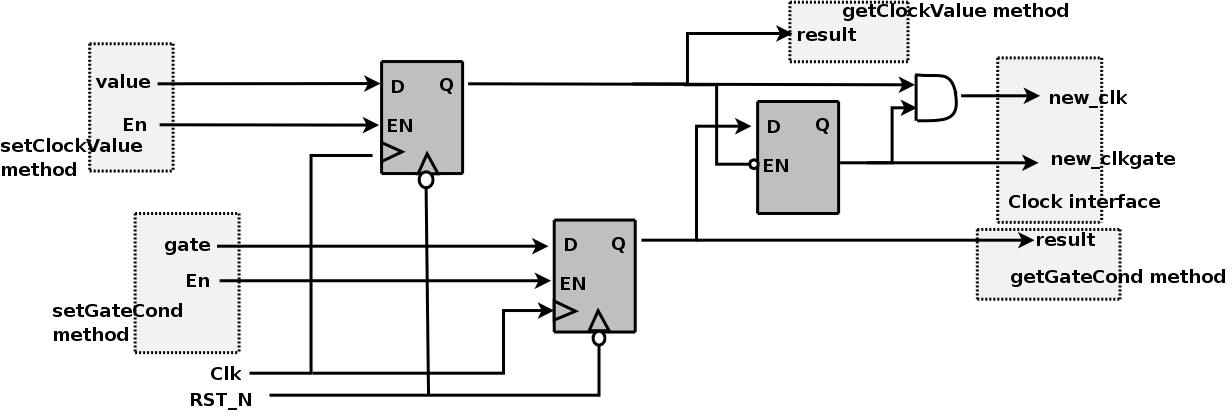
\includegraphics[width = 5 in]{LibFig/makeclock}
\caption{Clock Generator}
\label{makeclock}
\end{center}
\end{figure}


\index[function]{Clocks!mkClock}
\index{mkClock@\te{mkClock} (module)}
\begin{center}
\begin{tabular}{|p{1 in}|p{4.6 in}|}
\hline
&\\
\te{mkClock}&Creates a Clock type from a one-bit oscillator
input, and a Boolean gate condition.
There is no family relationship between the current clock and the clock
generated by this module.\\
\cline{2-2}
&\begin{libverbatim}
module mkClock #( one_bit_type initVal, Bool initGate) 
               ( MakeClockIfc#(one_bit_type) ifc )
   provisos( Bits#(one_bit_type, 1) ) ;
\end{libverbatim}
\\
\hline
\end{tabular}
\end{center}


\index[function]{Clocks!mkUngatedClock}
\index{mkUngatedClock@\te{mkUngatedClock} (module)}
\begin{center}
\begin{tabular}{|p{1 in}|p{4.6 in}|}
\hline
&\\
\te{mkUngatedClock}&Creates an ungated  Clock type from a one-bit oscillator
input.  There is no family relationship between the current clock and the clock
generated by this module.\\
\cline{2-2}
&\begin{libverbatim}
module mkUngatedClock #( one_bit_type initVal) 
               ( MakeClockIfc#(one_bit_type) ifc )
   provisos( Bits#(one_bit_type, 1) ) ;
\end{libverbatim}
\\
\hline
\end{tabular}
\end{center}

\index[function]{Clocks!mkGatedClock}
\index{mkGatedClock@\te{mkGatedClock} (module)}
 The \te{mkGatedClock} module adds (logic and) a Boolean gate condition
 to an existing clock, thus creating another clock in the same family.
 The source clock is provided as the argument \te{clk\_in}.
 The gate condition is controlled by an asynchronously-reset register
 inside the module.  The register is set with the \te{setGateCond} Action
 method of the interface and can be read with \te{getGateCond} method.
 The reset value of the gate condition register is provided as an
 instantiation parameter.  The clock for the register (and thus these set
 and get methods) is the default clock of the module; to specify a clock
 other than the default clock, use the \te{clocked\_by} directive.  

\begin{figure}[ht]
\begin{center}
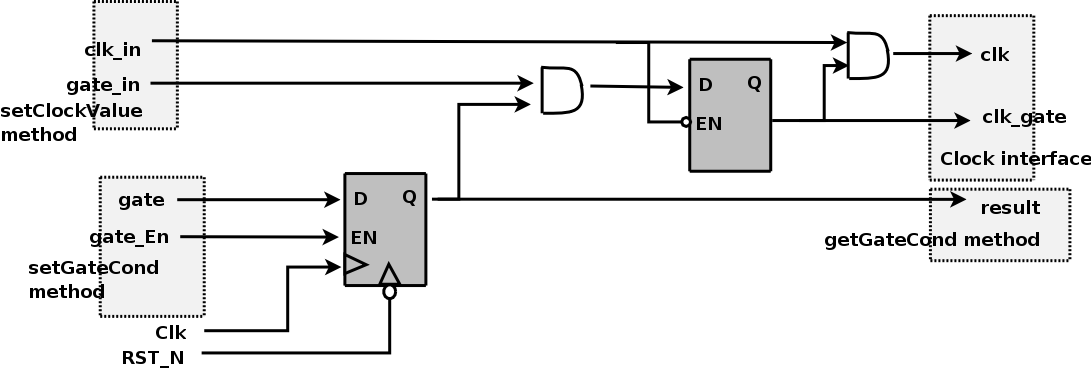
\includegraphics[width = 5 in]{LibFig/gatedclock}
\caption{Gated Clock Generator}
\label{gatedclock}
\end{center}
\end{figure}

\begin{center}
\begin{tabular}{|p{.9 in}|p{4.7 in}|}
\hline
& \\
\te{mkGatedClock}& Creates another clock in the same family by adding
logic and a Boolean gate condition to the current clock.\\
\cline{2-2}
&\begin{libverbatim}
module mkGatedClock#(Bool v) ( Clock clk_in, GatedClockIfc ifc );
\end{libverbatim}
\\ \hline
\end{tabular}
\end{center}

 For convenience, we provide an alternate version in which the source
 clock is the default clock of the module

\index[function]{Clocks!mkGatedClockFromCC}
\index{mkGatedClockFromCC@\te{mkGateClockFromCC} (module)}
\begin{center}
\begin{tabular}{|p{1.3 in}|p{4.3 in}|}
\hline
&\\
\te{mkGatedClockFromCC}&An alternate interface for the module
\te{mkGatedClock} in which the source clock is the default clock of
the module.\\
\cline{2-2}
&\begin{libverbatim}
module mkGatedClockFromCC#(Bool v) ( GatedClockIfc ifc );
\end{libverbatim}
\\
\hline
\end{tabular}
\end{center}

The modules \te{mkAbsoluteClock} and \te{mkAbsoluteClockFull}  provide
parametizable clock generation modules which are \emph{not}
synthesizable, but may be useful for testbenches.  In
\te{mkAbsoluteClock}, the first rising edge (start) and the
period are defined by parameters.  These parameters are measured in
Verilog delay times, which are usually specified during simulation
with the \te{timescale} directive.  Refer to the Verilog LRM for more
details on delay times. s Additional parameters are provided
by \te{mkAbsoluteClockFull}.  

\index{mkAbsoluteClock@\te{mkAbsoluteClock} (module)}
\index[function]{Clocks!mkAbsoluteClock}
\begin{center}
\begin{tabular}{|p{1.4 in}|p{4.2 in}|}
\hline
&\\
\te{mkAbsoluteClock}& The first rising edge (start) and period are
defined by parameters.  This module is not synthesizable.  \\
\cline{2-2}
&\begin{libverbatim}
module mkAbsoluteClock #( Integer start,
                          Integer period )
                          ( Clock );

\end{libverbatim}
\\
\hline
\end{tabular}
\end{center}

\index[function]{Clocks!mkAbsoluteClockFull}
\index{mkAbsoluteClockFull@\te{mkAbsoluteClockFull} (module)}
\begin{center}
\begin{tabular}{|p{1.4 in}|p{4.2 in}|}
\hline
&\\
\te{mkAbsoluteClockFull}& The value \te{initValue} is held until time \te{start}, and then the clock
oscillates.  The value \te{not(initValue)} is held for time
\te{compValTime}, followed by \te{initValue} held for time
\te{initValTime}.  Hence the clock period after startup is
\te{compValTime + initValTime}.   This module is not synthesizable.
 \\
\cline{2-2}
&\begin{libverbatim}
module mkAbsoluteClockFull #( Integer start, 
                              Bit#(1) initValue, 
                              Integer compValTime, 
                              Integer initValTime )
                              ( Clock );
\end{libverbatim}
\\
\hline
\end{tabular}
\end{center}



{\bf Verilog Modules}

The {\BSV} modules correspond to the following {\V}
modules, which are found in the BSC {\V} library, \te{\$BLUESPECDIR/Verilog/}.

\begin{center}
\begin{tabular}{|p {2.8 in}|p{2.8 in}|}
\hline
&\\
BSV Module Name & Verilog Module Name  \\
&\\
\hline
\hline
\te{mkAbsoluteClock}&\te{ClockGen.v} \\
\te{mkAbsoluteClockFull}& \\
\hline
\te{mkClock}&\te{MakeClock.v}\\
\te{mkUngatedClock}&\\
\hline
\te{mkGatedClock}&\te{GatedClock.v}\\
\te{mkGatedClockFromCC}&\\
\hline
\end{tabular}
\end{center}

%==========================================================================
\subsubsection{Clock Multiplexing}
\index{MuxClockIfc@\te{MuxClockIfc} (interface)}
\index{SelectClockIfc@\te{SelectClockIfc} (interface)}

{\bf Description}

BSC provides two gated clock multiplexing primitives:  a simple
combinational multiplexor and a stateful module which generates an
appropriate reset signal when the clock changes.  The first
multiplexor uses the interface \te{MuxClockIfc}, which  includes an
\te{Action} method to select the clock along with a \te{Clock}
subinterface.   The second multiplexor uses the interface
\te{SelectClockIfc} which also has  a \te{Reset} subinterface. 

Ungated versions of these modules are also provided.  The ungated
versions are identical to the gated versions, except that the input
and output clocks are ungated.  

{\bf Interfaces and Methods}

\begin{center}
\begin{tabular}{|p{.7in}|p{.7in}|p{1.8 in}|p{.4in}|p{1.4 in}|}
\hline
\multicolumn{5}{|c|}{MuxClockIfc Interface}\\
\hline
\multicolumn{3}{|c|}{Method and subinterfaces}&\multicolumn{2}{|c|}{Arguments}\\
\hline
Name & Type & Description& Name &\multicolumn{1}{|c|}{Description} \\
\hline
\hline 
\te{select}&\te{Action}&Method used to select the clock based on the
Boolean value {\tt ab} &{\tt ab}&if True, {\tt clock\_out} is taken
from {\tt aclk} \\
\hline
\te{clock\_out}&\te{Interface}&Clock interface&&\\
\hline
\end{tabular}
\end{center}


\begin{libverbatim}
     interface MuxClkIfc ;
        method    Action select ( Bool  ab ) ;
        interface Clock  clock_out ;
     endinterface
\end{libverbatim}

\begin{center}
\begin{tabular}{|p{.7in}|p{.7in}|p{1.8 in}|p{.4in}|p{1.4 in}|}
\hline
\multicolumn{5}{|c|}{SelectClockIfc Interface}\\
\hline
\multicolumn{3}{|c|}{Method and subinterfaces}&\multicolumn{2}{|c|}{Arguments}\\
\hline
Name & Type & Description& Name &\multicolumn{1}{|c|}{Description} \\
\hline
\hline 
\te{select}&\te{Action}&Method used to select the clock based on the
Boolean value {\tt ab} &{\tt ab}&if True, clock\_out is taken
from {\tt aclk} \\
\hline
\te{clock\_out}&\te{Interface}&Clock interface&&\\
\hline
\te{reset\_out}&\te{Interface}&Reset interface&&\\
\hline
\end{tabular}
\end{center}

\begin{libverbatim}
     interface SelectClkIfc ;
        method    Action select ( Bool  ab ) ;
        interface Clock  clock_out ;
        interface Reset  reset_out ;
     endinterface
\end{libverbatim}



{\bf Modules}

The \te{mkClockMux} module is a simple combinational multiplexor with
a registered clock selection signal,
which selects between clock inputs {\tt aClk} and {\tt bClk}.  The
provided  Verilog module
does not provide any glitch detection or removal logic;  it is the
responsibility of the user to provide additional logic to provide
glitch-free behavior.   The  \te{mkClockMux} module uses two
arguments and provides a Clock interface. The {\tt aClk} is selected if
{\tt ab} is True, while {\tt bClk} is selected otherwise.   

The \te{mkUngatedClockMux} module is identical to the \te{mkClockMux}
module except that the input and output clocks are ungated.  The
signals \te{aClkgate}, \te{bClkgate}, and \te{outClkgate} in figure
\ref{clockmux} don't exist.

\begin{figure}[ht]
\begin{center}
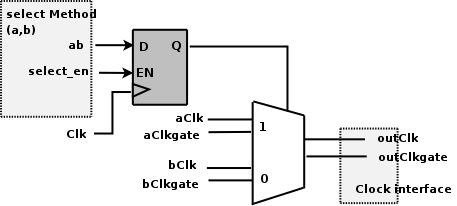
\includegraphics[height=1.4 in]{LibFig/clockmux}
\caption{Clock Multiplexor}
\label{clockmux}
\end{center}
\end{figure}


\index{mkClockMux@\te{mkClockMux} (module)}
\index[function]{Clocks!mkClockMux}
\begin{center}
\begin{tabular}{|p{1.4 in}|p{4.2 in}|}
\hline
&\\
\te{mkClockMux}&Simple combinational multiplexor,
which selects between aClk and bClk.\\
\cline{2-2}
&\begin{libverbatim}
module mkClockMux ( Clock aClk, Clock bClk )
                  ( MuxClkIfc ) ;
\end{libverbatim}
\\
\hline
\end{tabular}
\end{center}


\index{mkUngatedClockMux@\te{mkUngatedClockMux} (module)}
\index[function]{Clocks!mkUngatedClockMux}
\begin{center}
\begin{tabular}{|p{1.4 in}|p{4.2 in}|}
\hline
&\\
\te{mkUngatedClockMux}&Simple combinational multiplexor,
which selects between aClk and bClk.  None of the clocks are gated.\\
\cline{2-2}
&\begin{libverbatim}
module mkUngatedClockMux ( Clock aClk, Clock bClk )
                         ( MuxClkIfc ) ;
\end{libverbatim}
\\
\hline
\end{tabular}
\end{center}

\index{mkUngatedClockSelect@\te{mkUngatedClockSelect} (module)}
\index[function]{Clocks!mkUngatedClockSelect}
\index{mkClockSelect@\te{mkClockSelect} (module)}
\index[function]{Clocks!mkClockSelect}


The \te{mkClockSelect} module is a clock multiplexor 
containing additional logic which generates a reset whenever a new
clock is selected.  As such, the interface for the module includes
an \te{Action} method to select the clock (if {\tt ab} is True
clock\_out is taken from {\tt aClk}),
provides a \te{Clock} interface, and also a \te{Reset}
interface. 

The constructor for the module uses two clock arguments, and
provides the \te{MuxClockIfc} interface.  The underlying Verilog
module is {\tt ClockSelect.v};  it is expected that users can
substitute their own modules to meet any additional requirements
they may have.  The parameter {\tt stages} is the number of clock
cycles in which the reset is asserted after the clock selection changes.

The \te{mkUngatedClockSelect} module is identical to the \te{mkClockSelect}
module except that the input and output clocks are ungated.  The
signals \te{aClkgate}, \te{bClkgate}, and \te{outClk\_gate} in figure
\ref{clockselect} don't exist.


\begin{figure}[ht]
\begin{center}
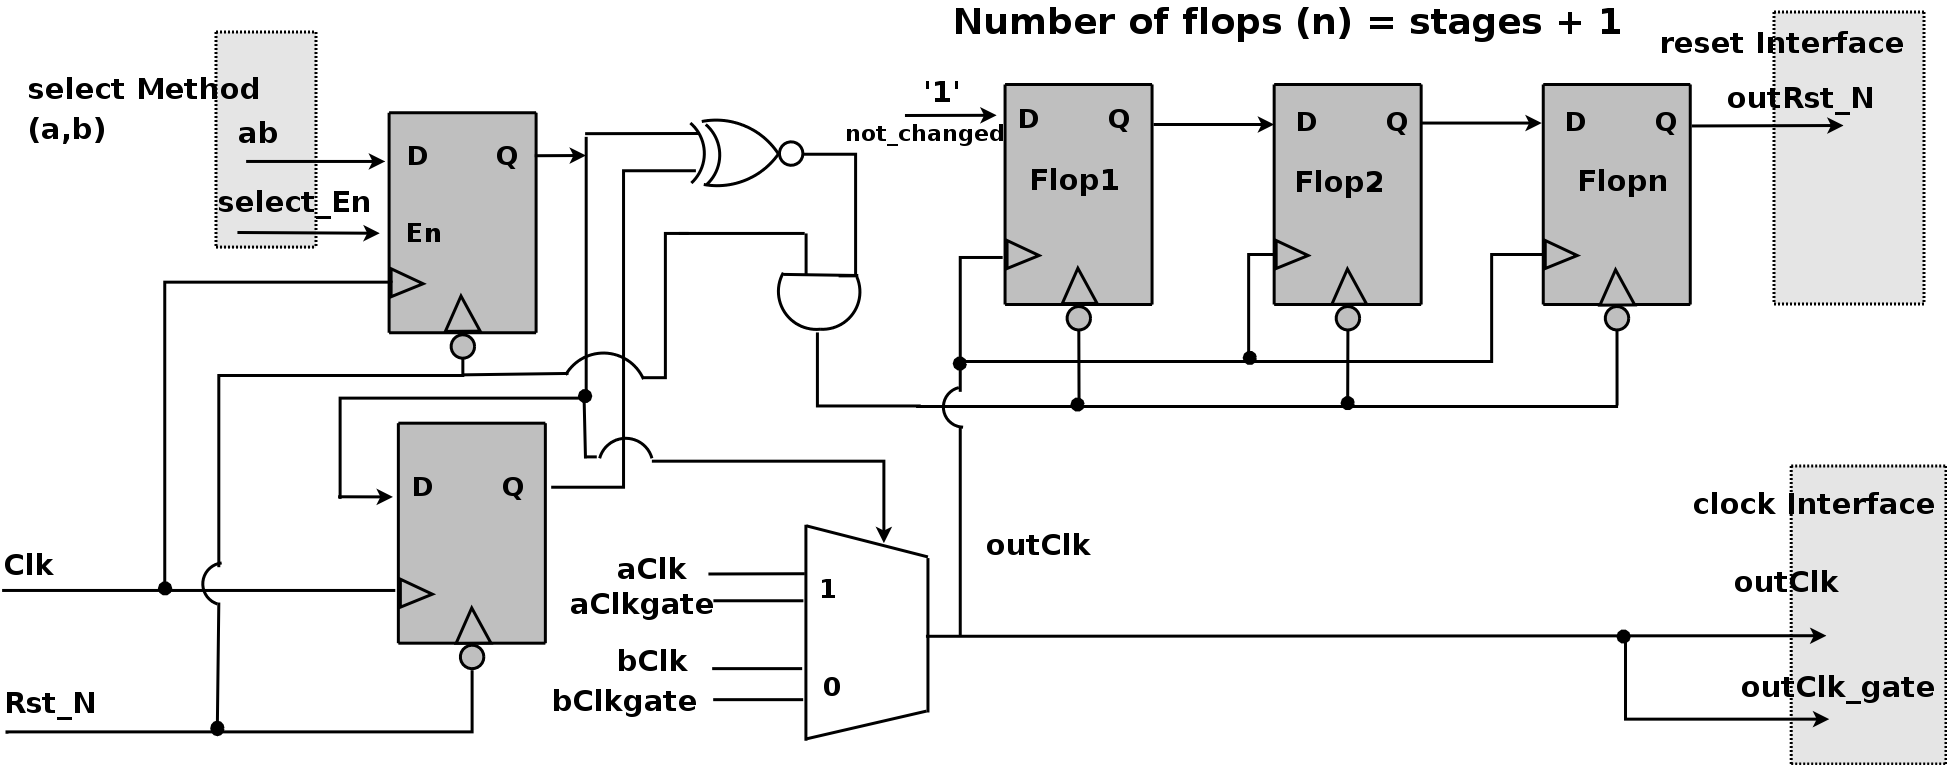
\includegraphics[width = 6 in]{LibFig/clockselect}
\caption{Clock Multiplexor with reset}
\label{clockselect}
\end{center}
\end{figure}



\begin{center}
\begin{tabular}{|p{1.4 in}|p{4.2 in}|}
\hline
&\\
\te{mkClockSelect}&Clock Multiplexor containing additional logic
which generates a reset whenever a new clock is selected.\\
\cline{2-2}
&\begin{libverbatim}
module mkClockSelect #( Integer stages, 
                          Clock aClk, 
                          Clock bClk, 
                        ( SelectClockIfc ) ;
\end{libverbatim}
\\
\hline
\end{tabular}
\end{center}      


\begin{center}
\begin{tabular}{|p{1.4 in}|p{4.2 in}|}
\hline
&\\
\te{mkUngatedClockSelect}&Clock Multiplexor containing additional logic
which generates a reset whenever a new clock is selected. The input
and output clocks are ungated.\\
\cline{2-2}
&\begin{libverbatim}
module mkUngatedClockSelect #( Integer stages, 
                               Clock aClk, 
                               Clock bClk, 
                             ( SelectClockIfc ) ;
\end{libverbatim}
\\
\hline
\end{tabular}
\end{center}      


   
{\bf Verilog Modules}

The {\BSV} modules correspond to the following {\V}
modules, which are found in the BSC {\V} library, \te{\$BLUESPECDIR/Verilog/}.


\begin{center}
\begin{tabular}{|p {2.8 in}|p{2.8 in}|}
\hline
&\\
BSV Module Name & Verilog Module Name  \\
&\\
\hline
\hline
\te{mkClockMux}& {\tt ClockMux.v} \\
\hline
\te{mkClockSelect}&{\tt ClockSelect.v}\\
\hline
\te{mkUngatedClockMux}& {\tt UngatedClockMux.v} \\
\hline
\te{mkUngatedClockSelect}&{\tt UngatedClockSelect.v}\\
\hline
\end{tabular}
\end{center}   
%======================================================================
\subsubsection{Clock Division}
\label{sec-clockdivider}
\index{ClockDividerIfc@\te{ClockDividerIfc} (interface)}
\index{mkClockDivider@\te{mkClockDivider} (module)}
\index{mkGatedClockDivider@\te{mkGatedClockDivider} (module)}
\index{mkClockDividerOffset@\te{mkClockDividerOffset} (module)}
\index{mkClockInverter@\te{mkClockInverter} (module)}
\index{mkGatedClockInverter@\te{mkGatedClockInverter} (module)}
\index[function]{Clocks!mkClockDivider}
\index[function]{Clocks!mkGatedClockDivider}
\index[function]{Clocks!mkClockInverter}
\index[function]{Clocks!mkGatedClockInverter}
\index[function]{Clocks!mkClockDividerOffset}
      
{\bf Description}

A clock divider provides a derived clock and also a \te{ClkNextRdy}
signal, which indicates that the divided
clock will rise in the next cycle.  This signal is associated with
the input clock, and can only be used within that clock domain.
     
The \te{AlignedFIFOs} package (Section \ref{sec-AlignedFIFOs})
contains parameterized FIFO modules for 
creating synchronizing FIFOs between clock domains with aligned edges.

% See {\tt mkSyncRegToSlow}, {\tt mkSyncRegToFast}, {\tt
%  mkSyncFIFOToSlow}, and {\tt mkSyncFIFOToFast} in Section
%  \ref{crossing-prim}
%  for some specialized synchronizers
% which can be used with divided clocks, and other systems when the
% clock edges are known to be aligned.
      
{\bf Data Types}

The \te{ClkNextRdy} is a Boolean 
signal which indicates that the slow
clock will rise in the next cycle.

\begin{libverbatim}
     typedef Bool ClkNextRdy ;
\end{libverbatim}

{\bf Interfaces and Methods}

\begin{center}
\begin{tabular}{|p{.7in}|p{.7in}|p{3.6 in}|}
\hline
\multicolumn{3}{|c|}{ClockDividerIfc Interface}\\
\hline
Name & Type & Description\\
\hline
\hline 
\te{fastClock}&\te{Interface}&The original clock\\
\hline
\te{slowClock}&\te{Interface}&The derived clock\\
\hline
\te{clockReady}&\te{Bool}&Boolean value which indicates that the
slow clock will rise in the next cycle.  The method is in the clock
domain of the fast clock.\\
\hline
\end{tabular}
\end{center}

\begin{libverbatim}
     interface ClockDividerIfc ;
         interface Clock      fastClock ;           
         interface Clock      slowClock ;           
         method    ClkNextRdy clockReady() ;        
     endinterface 
\end{libverbatim}

{\bf Modules}

The {\tt divider} parameter may be any integer greater than 1.
For even dividers the generated clock's duty cycle is 50\%, while
for odd dividers, the duty cycle is $(divider/2) / divider$.  Since
\te{divisor} is an integer, the remainder is truncated when divided.   The
current clock (or the \te{clocked\_by} argument) is used as the
source clock.  

\begin{figure}[ht]
\begin{center}
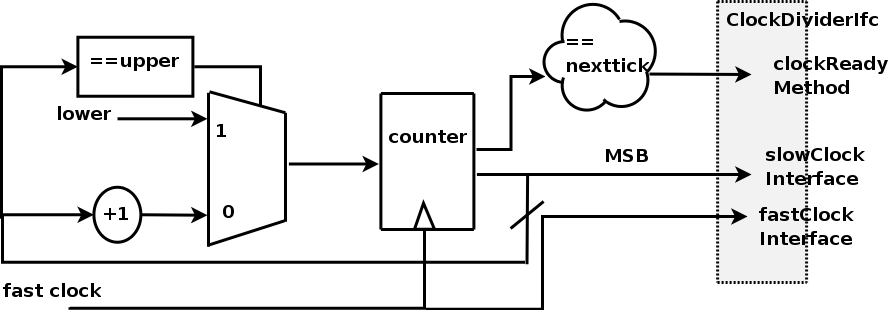
\includegraphics[height=1.2 in]{LibFig/clockdiv}
\caption{Clock Divider}
\label{clockdiv}
\end{center}
\end{figure}


\begin{center}
\begin{tabular}{|p{1.6 in}|p{4.0 in}|}
\hline
&\\
\te{mkClockDivider}& Basic clock divider.\\
\cline{2-2}
&\begin{libverbatim}
module mkClockDivider #( Integer divisor ) 
                       ( ClockDividerIfc ) ;
\end{libverbatim}
\\
\hline
\end{tabular}
\end{center}


\begin{center}
\begin{tabular}{|p{1.6 in}|p{4.0 in}|}
\hline
&\\
\te{mkGatedClockDivider}& A gated verison of the basic clock divider.\\
\cline{2-2}
&\begin{libverbatim}
module mkGatedClockDivider #( Integer divisor 
                            )( ClockDividerIfc ) ;
\end{libverbatim}
\\
\hline
\end{tabular}
\end{center}



The {\tt  mkClockDividerOffset} module provides a clock divider 
where the rising edge can be defined relative to other clock
dividers which have the same divisor.  An offset of value 2 will
produce a rising edge one fast clock after a divider with offset
1.  \te{mkClockDivider} is just \te{mkClockDividerOffset} with an
offset of value 0. 

\begin{center}
\begin{tabular}{|p{1.6 in}|p{4.0 in}|}
\hline
&\\
\te{mkClockDividerOffset}&Provides a clock divider,
where the rising edge can be defined relative to other clock
dividers which have the same divisor.\\
\cline{2-2}
&\begin{libverbatim}
module mkClockDividerOffset #( Integer divisor, 
                               Integer offset )
                             ( ClockDividerIfc ) ;
\end{libverbatim}
\\
\hline
\end{tabular}
\end{center}


The \te{mkClockInverter} and \te{mkGatedClockInverter} modules
generate an inverted clock having the same period but opposite phase
as the current clock.  The \te{mkGatedClockInverter} is a gated
version of \te{mkClockInverter}.  The output
clock includes a gate signal derived from the gate of the input clock.
 
\begin{center}
\begin{tabular}{|p{1.6 in}|p{4.0 in}|}
\hline
&\\
\te{mkClockInverter}&Generates an inverted clock having
the same period but opposite phase as the current clock.\\
\cline{2-2}
&\begin{libverbatim}
module mkClockInverter ( ClockDividerIfc ) ;
\end{libverbatim}     
\\
\hline
\end{tabular}
\end{center} 


\begin{center}
\begin{tabular}{|p{1.6 in}|p{4.0 in}|}
\hline
&\\
\te{mkGatedClockInverter}&A gated version of \te{mkClockInverter}.
\\
\cline{2-2}
&\begin{libverbatim}
module mkGatedClockInverter ( ClockDividerIfc ifc ) ;
\end{libverbatim}     
\\
\hline
\end{tabular}
\end{center} 

{\bf Verilog Modules}

The {\BSV} modules correspond to the following {\V}
modules, which are found in the BSC {\V} library, \te{\$BLUESPECDIR/Verilog/}.


\begin{center}
\begin{tabular}{|p {2.8 in}|p{2.8 in}|}
\hline
&\\
BSV Module Name & Verilog Module Name  \\
&\\
\hline
\hline
{\tt mkClockDivider}& \te{ClockDiv.v}\\
{\tt mkClockDividerOffset}&\\
\hline
{\tt mkGatedClockDivider}&\te{GatedClockDiv.v}\\
\hline
{\tt mkClockInverter}&\te{ClockInverter.v}\\
\hline
{\tt mkGatedClockInverter}&\te{GatedClockInverter.v}\\
\hline
\end{tabular}
\end{center}

%=====================================================================
\subsubsection{Bit Synchronizers}

\index{SyncBitIfc@\te{SyncBitIfc} (interface)}

{\bf Description}

Bit synchronizers are used to safely transfer one bit of data from one
clock domain to another.  More complicated synchronizers are provided
in later sections.

{\bf Interfaces and Methods}

The  {\tt SyncBitIfc} interface provides a \te{send} method
which  transmits
one bit of information from one clock domain to the \te{read}
method in a second domain.

\begin{center}
\begin{tabular}{|p{.4in}|p{.8 in}|p{1.8 in}|p{.6in}|p{1.4 in}|}
\hline
\multicolumn{5}{|c|}{SyncBitIfc Interface}\\
\hline
\multicolumn{3}{|c|}{Methods}&\multicolumn{2}{|c|}{Arguments}\\
\hline
Name & Type & Description& Name &\multicolumn{1}{|c|}{Description} \\
\hline
\hline 
\te{send}&\te{Action}&Transmits information from one clock
domain to the second domain&\te{bitData}&One bit of information transmitted \\
\hline
\te{read}&\te{one\_bit\_type}&Reads one bit of data sent from a
different clock domain&&\\
\hline
\end{tabular}
\end{center}


\begin{libverbatim}
     interface SyncBitIfc #(type one_bit_type) ;
        method Action       send ( one_bit_type bitData ) ;
        method one_bit_type read () ;
     endinterface
\end{libverbatim}



{\bf Modules}

The \te{mkSyncBit}, \te{mkSyncBitFromCC} and \te{mkSyncBitToCC}
modules provide a \te{SyncBitIfc} across clock domains.  The send
method is in  one clock domain, and the read method is in
a second clock domain, as shown in Figure \ref{bitsynch}.  The
\te{FromCC}  and \te{ToCC} versions
differ in that the \te{FromCC} module moves data {\em{from}} the current clock
(module's clock), while
the \te{ToCC} module moves data {\em{to}} the current clock domain.
The  hardware implementation is a two
register synchronizer, which can be found in \te{SyncBit.v} in the
BSC {\V} library directory.
 

\begin{figure}[ht]
\begin{center}
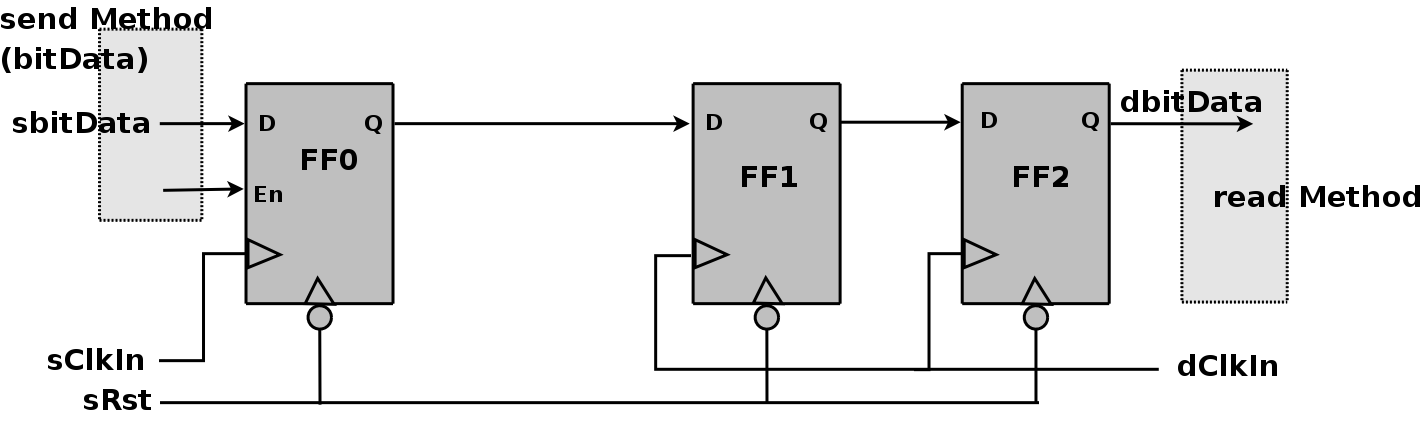
\includegraphics[height=1.2 in]{LibFig/bitsynch}
\caption{Bit Synchronizer}
\label{bitsynch}
\end{center}
\end{figure}


\index{mkSyncBit@\te{mkSyncBit} (module)}
\index[function]{Clocks!mkSyncBit}
\begin{center}
\begin{tabular}{|p{1.4 in}|p{4.2 in}|}
\hline
&\\
\te{mkSyncBit}&Moves data across clock domains.  The in and out clocks,
along with the input reset, are explicitly provided.  The default clock
and reset are ignored.\\
\cline{2-2}
&\begin{libverbatim}
module mkSyncBit #( Clock sClkIn, Reset sRst, 
                    Clock dClkIn ) 
                  ( SyncBitIfc #(one_bit_type) )
   provisos( Bits#(one_bit_type, 1)) ;
\end{libverbatim}     
\\
\hline
\end{tabular}
\end{center} 

\index[function]{Clocks!mkSyncBitFromCC}
\index{mkSyncBitFromCC@\te{mkSyncBitFromCC} (module)}
\begin{center}
\begin{tabular}{|p{1.4 in}|p{4.2 in}|}
\hline
&\\
\te{mkSyncBitFromCC}&Moves data from the current clock (the module's
clock) to a different clock domain. The input clock and reset are the
current clock and reset.  \\
\cline{2-2}
&\begin{libverbatim}
module mkSyncBitFromCC #( Clock dClkIn )
                        ( SyncBitIfc #(one_bit_type) ) 
   provisos( Bits#(one_bit_type, 1)) ;
\end{libverbatim}     
\\
\hline
\end{tabular}
\end{center} 

\index[function]{Clocks!mkSyncBitToCC}
\index{mkSyncBitToCC@\te{mkSyncBitToCC} (module)}
\begin{center}
\begin{tabular}{|p{1.4 in}|p{4.2 in}|}
\hline
&\\
\te{mkSyncBitToCC}&Moves data into the current clock domain. The
output clock is the current clock. The current reset is ignored. \\
\cline{2-2}
&\begin{libverbatim}
module mkSyncBitToCC #( Clock sClkIn, Reset sRstIn )
                      ( SyncBitIfc #(one_bit_type) ) 
   provisos( Bits#(one_bit_type, 1)) ;
\end{libverbatim}     
\\
\hline
\end{tabular}
\end{center} 

\index[function]{Clocks!mkSyncBit15}
\index{mkSyncBit15@\te{mkSyncBit15} (module)}
The \te{mkSyncBit15} module (one and a half) and its variants provide the same
interface as the \te{mkSyncBit} modules, but the underlying
hardware is slightly modified, as shown in Figure \ref{bitsynch15}. For these synchronizers, the first
register clocked by the destination clock triggers on the falling
edge of the clock.  
   
\begin{figure}[ht]
\begin{center}
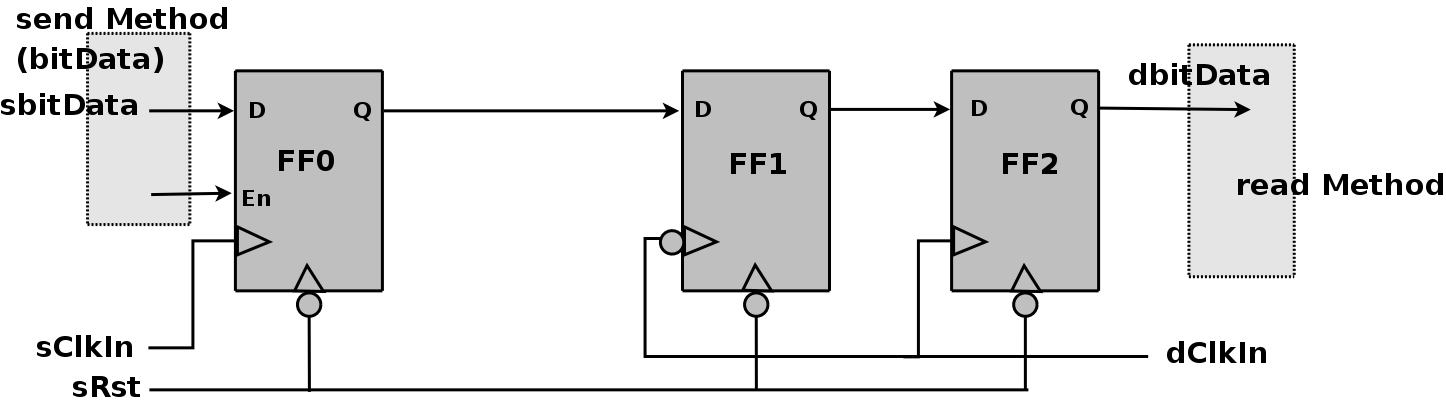
\includegraphics[height=1.2 in]{LibFig/bitsynch15}
\caption{Bit Synchronizer 1.5 - first register in destination domain
triggers  on falling edge}
\label{bitsynch15}
\end{center}
\end{figure}


\begin{center}
\begin{tabular}{|p{1.4 in}|p{4.2 in}|}
\hline
&\\
\te{mkSyncBit15}&Similar to \te{mkSyncBit} except it
 triggers on the falling edge of the clock. The in and out clocks,
along with the input reset, are explicitly provided.  The default clock
and reset are ignored.   \\
\cline{2-2}
&\begin{libverbatim}
module mkSyncBit15 #( Clock sClkIn, Reset sRst, 
                      Clock dClkIn )
                    ( SyncBitIfc #(one_bit_type) ) 
   provisos( Bits#(one_bit_type, 1)) ;
\end{libverbatim}     
\\
\hline
\end{tabular}
\end{center} 

\index[function]{Clocks!mkSyncBit15FromCC}
\index{mkSyncBit15FromCC@\te{mkSyncBit15FromCC} (module)}
\begin{center}
\begin{tabular}{|p{1.4 in}|p{4.2 in}|}
\hline
&\\
\te{mkSyncBit15FromCC}&Moves data from the current clock and is
triggered on the falling edge of the clock. The input clock and reset are the
current clock and reset. \\
\cline{2-2}
&\begin{libverbatim}
module mkSyncBit15FromCC #(Clock dClkIn)
                          (SyncBitIfc #(one_bit_type)) 
   provisos( Bits#(one_bit_type, 1)) ;
\end{libverbatim}     
\\
\hline
\end{tabular}
\end{center} 

\index[function]{Clocks!mkSyncBit15ToCC}
\index{mkSyncBit15ToCC@\te{mkSyncBit15ToCC} (module)}
\begin{center}
\begin{tabular}{|p{1.4 in}|p{4.2 in}|}
\hline
&\\
\te{mkSyncBit15ToCC}&Moves data into the current clock domain and is
triggered on the falling edge of the clock. The
output clock is the current clock. The current reset is ignored. \\
\cline{2-2}
&\begin{libverbatim}
module mkSyncBit15ToCC #( Clock sClkIn, Reset sRstIn )
                        ( SyncBitIfc #(one_bit_type) ) 
   provisos( Bits#(one_bit_type, 1)) ;
\end{libverbatim}     
\\
\hline
\end{tabular}
\end{center} 

\index[function]{Clocks!mkSyncBit1}
\index{mkSyncBit1@\te{mkSyncBit1} (module)}
The \te{mkSyncBit1} module, shown in Figure \ref{bitsynch1}, also
provides the  same interface but
only uses one register in the destination domain.  Synchronizers
like this, which use only one
register, are not generally used since meta-stable output
is more probable.  However, one can use this synchronizer provided
special meta-stable resistant flops are selected during physical
synthesis or (for example) if the output is immediately registered.

\begin{figure}[ht]
\begin{center}
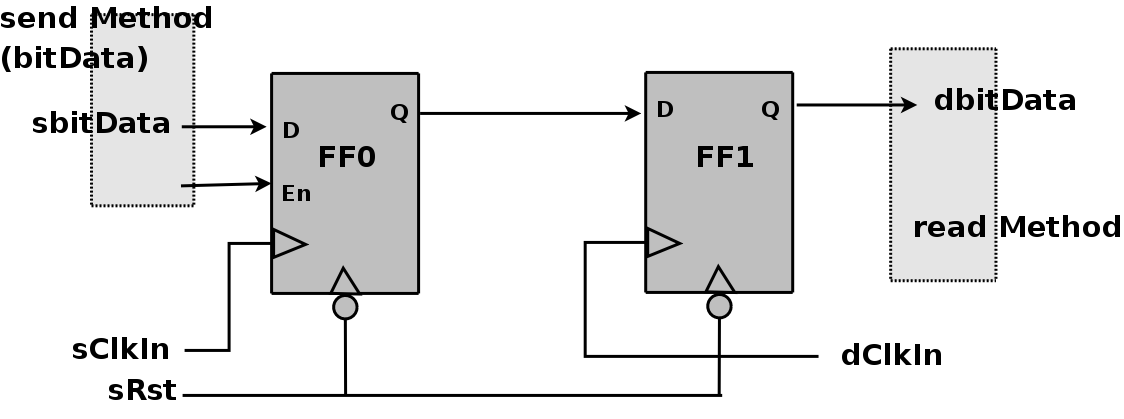
\includegraphics[height=1.2 in]{LibFig/bitsynch1}
\caption{Bit Synchronizer 1.0 - single register in destination domain}
\label{bitsynch1}
\end{center}
\end{figure}



\begin{center}
\begin{tabular}{|p{1.4 in}|p{4.2 in}|}
\hline
&\\
\te{mkSyncBit1}&Moves data from one clock domain to another clock
domain, with only one register in the destination domain. The in and out clocks,
along with the input reset, are explicitly provided.  The default clock
and reset are ignored. \\
\cline{2-2}
&\begin{libverbatim}
module mkSyncBit1 #( Clock sClkIn, Reset sRst,
                     Clock dClkIn )
                   ( SyncBitIfc #(one_bit_type) ) 
   provisos( Bits#(one_bit_type, 1)) ;
\end{libverbatim}     
\\
\hline
\end{tabular}
\end{center} 


\index[function]{Clocks!mkSyncBit1FromCC}
\index{mkSyncBit1FromCC@\te{mkSyncBit1FromCC} (module)}
\begin{center}
\begin{tabular}{|p{1.4 in}|p{4.2 in}|}
\hline
&\\
\te{mkSyncBit1FromCC}&Moves data from the current clock domain, with only one register in the destination domain. The input clock and reset are the
current clock and reset. \\
\cline{2-2}
&\begin{libverbatim}
module mkSyncBit1FromCC #( Clock dClkIn )
                         ( SyncBitIfc #(one_bit_type) ) 
   provisos( Bits #(one_bit_type, 1)) ;
\end{libverbatim}     
\\
\hline
\end{tabular}
\end{center} 

\index[function]{Clocks!mkSyncBit1ToCC}
\index{mkSyncBit1ToCC@\te{mkSyncBit1ToCC} (module)}
\begin{center}
\begin{tabular}{|p{1.4 in}|p{4.2 in}|}
\hline
&\\
\te{mkSyncBit1ToCC}& Moves data into the current clock domain, with
only one register in the destination domain. The
output clock is the current clock. The current reset is ignored.  \\
\cline{2-2}
&\begin{libverbatim}
module mkSyncBit1ToCC #( Clock sClkIn, Reset sRstIn )
                       ( SyncBitIfc #(one_bit_type) ) 
   provisos( Bits#(one_bit_type, 1)) ;
\end{libverbatim}     
\\
\hline
\end{tabular}
\end{center} 

%// A general module which not use the current clock or reset


The \te{mkSyncBit05} module is similar to \te{mkSyncBit1}, but the
destination  register
triggers on the falling edge of the clock, as shown in Figure \ref{bitsynch05}.


\begin{figure}[ht]
\begin{center}
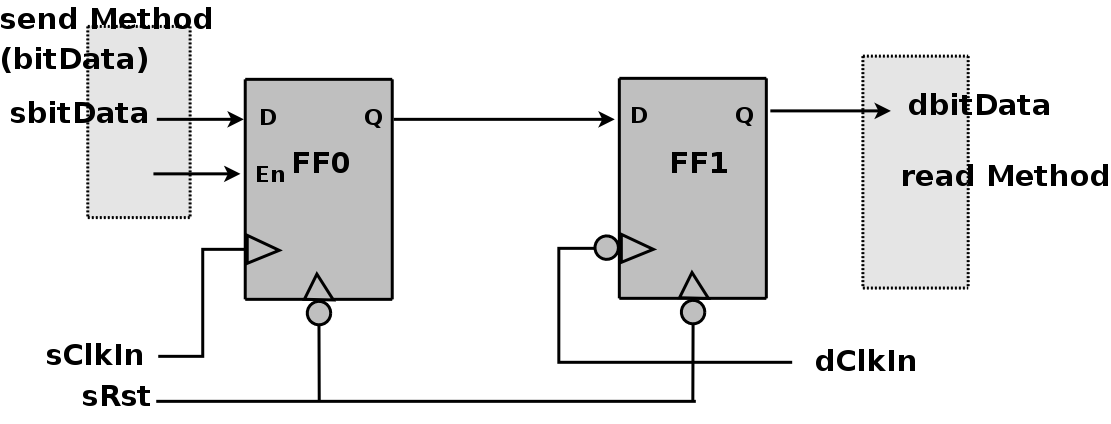
\includegraphics[height=1.2 in]{LibFig/bitsynch05}
\caption{Bit Synchronizer .5 - first register in destination domain
triggers on falling edge}
\label{bitsynch05}
\end{center}
\end{figure}

\index[function]{Clocks!mkSyncBit05}
\index{mkSyncBit05@\te{mkSyncBit05} (module)}
\begin{center}
\begin{tabular}{|p{1.4 in}|p{4.2 in}|}
\hline
&\\
\te{mkSyncBit05}&Moves data from one clock domain to another clock
domain, with only one register in the destination domain.  The destination register triggers on the falling edge of the clock. The in and out clocks,
along with the input reset, are explicitly provided.  The default clock
and reset are ignored.\\
\cline{2-2}
&\begin{libverbatim}
module mkSyncBit05 #( Clock sClkIn, Reset sRst, 
                      Clock dClkIn ) 
                    ( SyncBitIfc #(one_bit_type) ) 
   provisos( Bits#(one_bit_type, 1)) ;
\end{libverbatim}     
\\
\hline
\end{tabular}
\end{center} 

\index[function]{Clocks!mkSyncBit05FromCC}
\index{mkSyncBit05FromCC@\te{mkSyncBit05FromCC} (module)}   
\begin{center}
\begin{tabular}{|p{1.4 in}|p{4.2 in}|}
\hline
&\\
\te{mkSyncBit05FromCC}&Moves data from the current clock domain, with only one register
in the destination domain, the destination register triggers on the
falling edge of the clock.   The input clock and reset are the
current clock and reset.  \\
\cline{2-2}
&\begin{libverbatim}
module mkSyncBit05FromCC #( Clock dClkIn ) 
                          (SyncBitIfc #(one_bit_type) ) 
   provisos( Bits#(one_bit_type, 1)) ;
\end{libverbatim}     
\\
\hline
\end{tabular}
\end{center} 

\index[function]{Clocks!mkSyncBit05ToCC}
\index{mkSyncBit05ToCC@\te{mkSyncBit05ToCC} (module)}
\begin{center}
\begin{tabular}{|p{1.4 in}|p{4.2 in}|}
\hline
&\\
\te{mkSyncBit05ToCC}&Moves data into the current clock domain, with only one register
in the destination domain, the destination register triggers on the
falling edge of the clock.  The
output clock is the current clock. The current reset is ignored.    \\
\cline{2-2}
&\begin{libverbatim}
module mkSyncBit05ToCC #( Clock sClkIn, Reset sRstIn ) 
                        ( SyncBitIfc #(one_bit_type) ) 
   provisos( Bits#(one_bit_type, 1)) ;
\end{libverbatim}     
\\
\hline
\end{tabular}
\end{center} 

{\bf Verilog Modules}

The {\BSV} modules correspond to the following {\V}
modules, which are found in the BSC {\V} library, \te{\$BLUESPECDIR/Verilog/}.


\begin{center}
\begin{tabular}{|p {2.8 in}|p{2.8 in}|}
\hline
&\\
BSV Module Name & Verilog Module Name  \\
&\\
\hline
\hline
\te{mkSyncBit}& \te{SyncBit.v}\\
\te{mkSyncBitFromCC}&\\
\te{mkSyncBitToCC}&\\
\hline
\te{mkSyncBit15}&\te{SyncBit15.v}\\
\te{mkSyncBit15FromCC}&\\
\te{mkSyncBit15ToCC}&\\
\hline
\te{mkSyncBit1}&\te{SyncBit1.v}\\
\te{mkSyncBit1FromCC}&\\
\te{mkSyncBit1ToCC}&\\
\hline
\te{mkSyncBit05}&\te{SyncBit05.v}\\
\te{mkSyncBit05FromCC}&\\
\te{mkSyncBit05ToCC}&\\
\hline
\end{tabular}
\end{center}
%====================================================
\subsubsection{Pulse Synchronizers}
\index{SyncPulseIfc@\te{SyncPulseIfc} (interface)}

{\bf Description}

Pulse synchronizers are used to transfer a pulse from one clock domain
to another.


{\bf Interfaces and Methods}

The \te{SyncPulseIfc} interface provides an Action method, \te{send},
which  when
invoked generates a True value on the \te{pulse} method in a second clock domain.

\begin{center}
\begin{tabular}{|p{.4in}|p{.8 in}|p{3.6in}|}
\hline
\multicolumn{3}{|c|}{SyncPulseIfc Interface}\\
\hline
\multicolumn{3}{|c|}{Methods}\\
\hline
Name & Type & Description\\
\hline
\hline 
\te{send}&\te{Action}&Starts transmittling a pulse from one clock
domain to the second clock domain.\\
\hline
\te{pulse}&\te{Bool}&Where the pulse is received in the second domain.
\te{pulse} is True if a pulse is recieved in this cycle.\\
\hline
\end{tabular}
\end{center}

\begin{libverbatim}
     interface SyncPulseIfc ;
        method Action send  () ;
        method Bool   pulse () ;
     endinterface
\end{libverbatim}

{\bf Modules}

The \te{mkSyncPulse}, \te{mkSyncPulseFromCC} and \te{mkSyncPulseToCC} modules
provide clock domain crossing modules for pulses.  When the
\te{send} method is called from the one clock domain, a pulse will
be seen on the \te{read} method in the second.  Note that there is
no handshaking between the domains, so when sending data
from a fast clock domain to a slower one, not all pulses sent may
be seen in the slower receiving clock domain.  The pulse delay is
two destination clocks cycles.

\begin{figure}[ht]
\begin{center}
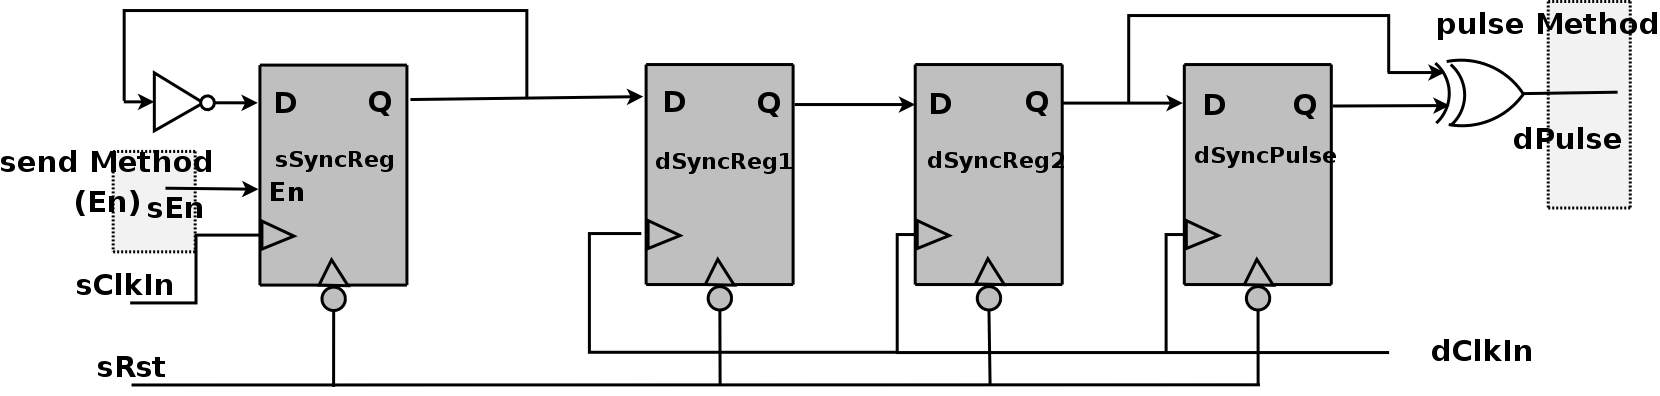
\includegraphics[width = 5 in]{LibFig/syncpulse}
\caption{Pulse Synchronizer - no handshake}
\label{syncpulse}
\end{center}
\end{figure}

\index[function]{Clocks!mkSyncPulse}
\index{mkSyncPulse@\te{mkSyncPulse} (module)}
\begin{center}
\begin{tabular}{|p{1.4 in}|p{4.2 in}|}
\hline
&\\
\te{mkSyncPulse}&Sends a pulse from one clock domain to another. The in and out clocks,
along with the input reset, are explicitly provided.  The default clock
and reset are ignored. \\
\cline{2-2}
&\begin{libverbatim}
module mkSyncPulse #( Clock sClkIn, Reset sRstIn, 
                      Clock dClkIn )
                    ( SyncPulseIfc ) ;
\end{libverbatim}     
\\
\hline
\end{tabular}
\end{center} 

\index[function]{Clocks!mkSyncPulseFromCC}
\index{mkSyncPulseFromCC@\te{mkSyncPulseFromCC} (module)}
\begin{center}
\begin{tabular}{|p{1.4 in}|p{4.2 in}|}
\hline
&\\
\te{mkSyncPulseFromCC}&Sends a pulse from the current clock domain to
the other clock domain. The input clock and reset are the
current clock and reset. \\
\cline{2-2}
&\begin{libverbatim}
module mkSyncPulseFromCC #( Clock dClkIn ) 
                          ( SyncPulseIfc ) ;
\end{libverbatim}     
\\
\hline
\end{tabular}
\end{center} 

\index[function]{Clocks!mkSyncPulseToCC}
\index{mkSyncPulseToCC@\te{mkSyncPulseToCC} (module)}
\begin{center}
\begin{tabular}{|p{1.4 in}|p{4.2 in}|}
\hline
&\\
\te{mkSyncPulseToCC}&Sends a pulse from the other clock domain to the
current clock domain.  The
output clock is the current clock. The current reset is ignored.  \\
\cline{2-2}
&\begin{libverbatim}
module mkSyncPulseToCC #( Clock sClkIn, Reset sRstIn ) 
                        ( SyncPulseIfc ) ;
\end{libverbatim}     
\\
\hline
\end{tabular}
\end{center} 

%\index[function]{Clocks!mkSyncHandshake}
%\index{mkSyncHandshake@\te{mkSyncHandshake} (module)}
The \te{mkSyncHandshake}, \te{mkSyncHandshakeFromCC} and \te{mkSyncHandshakeToCC} modules
provide clock domain crossing modules for pulses in a similar way
as \te{mkSyncPulse} modules, except that a handshake is provided
in the \te{mkSyncHandshake} versions. The handshake enforces that
another send does not occur before the first pulse crosses to the
other domain.  Note that this only guarantees that the pulse is seen
in one clock cycle of the destination; it does not guarantee that the
system on that side reacted to the pulse before it was gone.  It is up
to the designer to ensure this, if necessary.  The modules are not
ready in reset. 

The pulse delay from the \te{send} method to the \te{read} method
is two destination clocks.  The \te{send} method is re-enabled in
two destination clock cycles plus two source clock cycles after the
\te{send} method is called.  




\begin{figure}[ht]
\begin{center}
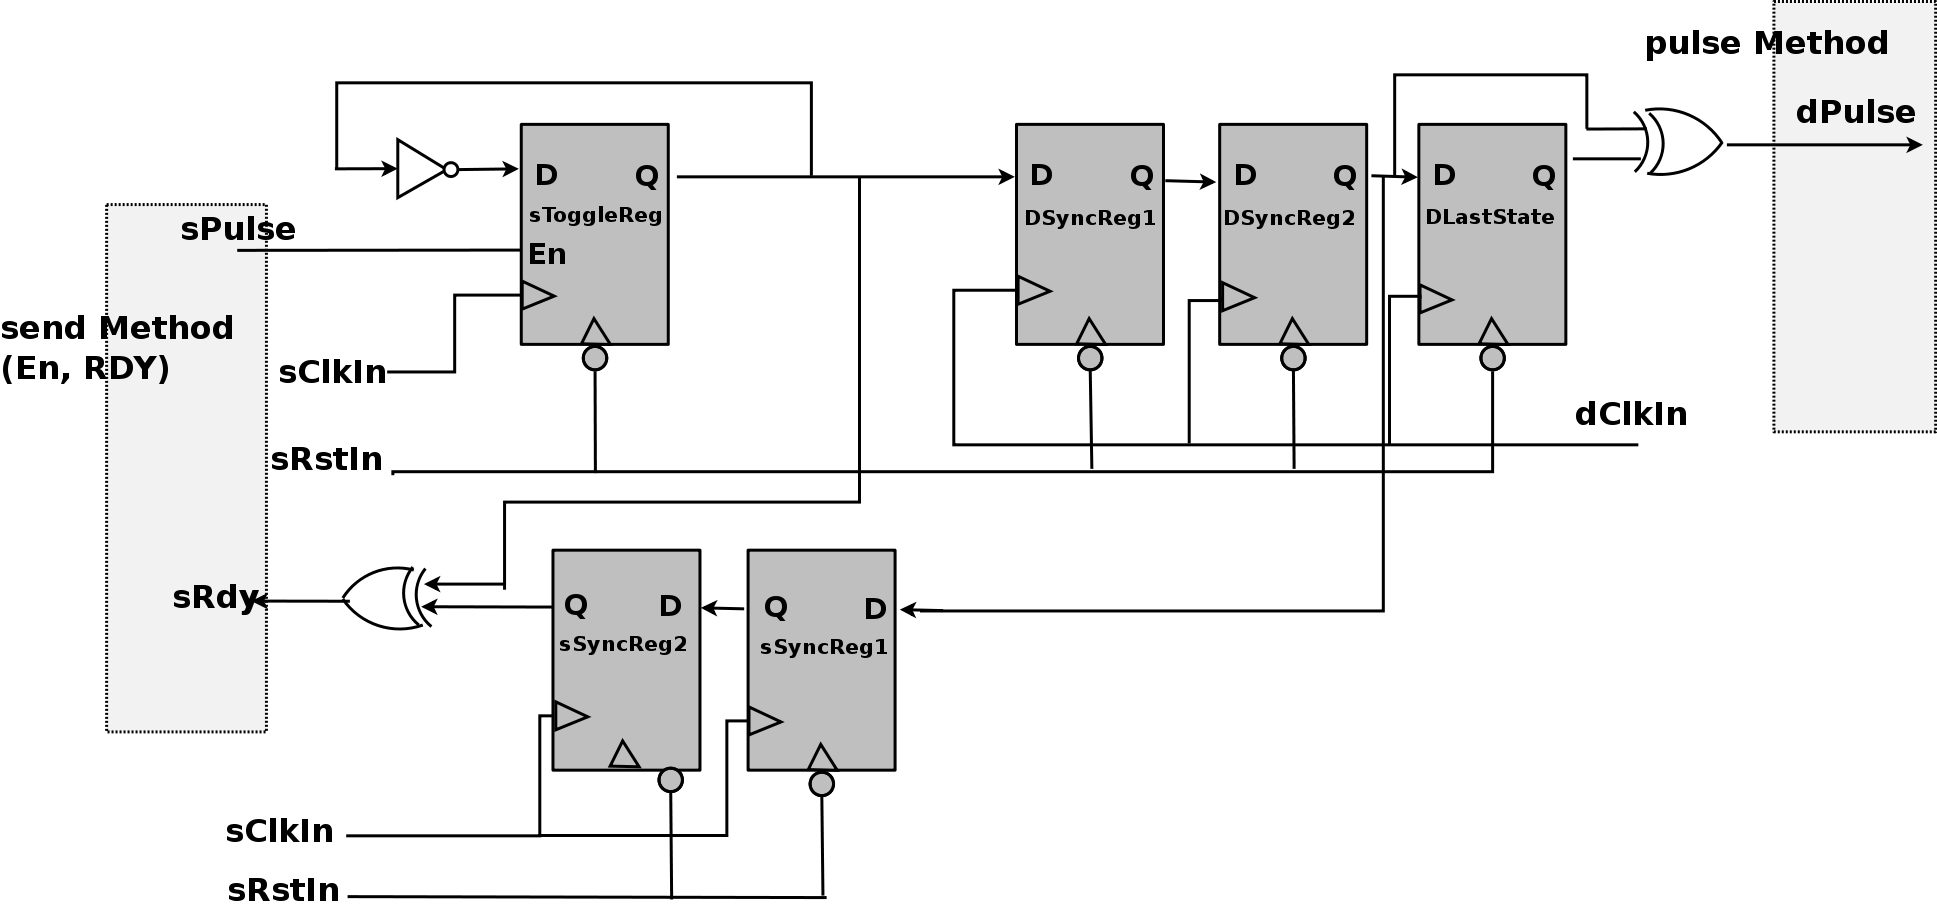
\includegraphics[width = 5.5 in]{LibFig/synchandshake}
\caption{Pulse Synchronizer with handshake}
\label{synchandshake}
\end{center}
\end{figure}


\index[function]{Clocks!mkSyncHandshake}
\index{mkSyncHandshake@\te{mkSyncHandshake} (module)}
\begin{center}
\begin{tabular}{|p{1.4 in}|p{4.2 in}|}
\hline
&\\
\te{mkSyncHandshake}&Sends a pulse from one clock domain to another
clock domain with handshaking.  The in and out clocks,
along with the input reset, are explicitly provided.  The default clock
and reset are ignored.  \\
\cline{2-2}
&\begin{libverbatim}
module mkSyncHandshake #( Clock sClkIn, Reset sRstIn, 
                          Clock dClkIn )
                        ( SyncPulseIfc ) ;
\end{libverbatim}     
\\
\hline
\end{tabular}
\end{center} 

\index[function]{Clocks!mkSyncHandshakeFromCC}
\index{mkSyncHandshakeFromCC@\te{mkSyncHandshakeFromCC} (module)}
\begin{center}
\begin{tabular}{|p{1.6 in}|p{4.0 in}|}
\hline
&\\
\te{mkSyncHandshakeFromCC}&Sends a pulse with a handshake from the
current clock domain. The input clock and reset are the
current clock and reset. \\
\cline{2-2}
&\begin{libverbatim}
module mkSyncHandshakeFromCC #( Clock dClkIn ) 
                              ( SyncPulseIfc ) ;
\end{libverbatim}     
\\
\hline
\end{tabular}
\end{center} 

\index[function]{Clocks!mkSyncHandshakeToCC}
\index{mkSyncHandshakeToCC@\te{mkSyncHandshakeToCC} (module)}
\begin{center}
\begin{tabular}{|p{1.6 in}|p{4.0 in}|}
\hline
&\\
\te{mkSyncHandshakeToCC}&Sends a pulse with a handshake to the current
clock domain.  The
output clock is the current clock. The current reset is ignored. \\
\cline{2-2}
&\begin{libverbatim}
module mkSyncHandshakeToCC #( Clock sClkIn, 
                              Reset sRstIn )
                            ( SyncPulseIfc ) ;
\end{libverbatim}     
\\
\hline
\end{tabular}
\end{center} 

{\bf Verilog Modules}

The {\BSV} modules correspond to the following {\V}
modules, which are found in the BSC {\V} library, \te{\$BLUESPECDIR/Verilog/}.

\begin{center}
\begin{tabular}{|p {2.8 in}|p{2.8 in}|}
\hline
&\\
BSV Module Name & Verilog Module Name  \\
&\\
\hline
\hline
\te{mkSyncPulse}&\te{SyncPulse.v} \\
\te{mkSyncPulseFromCC}&\\
\te{mkSyncPulseToCC}&\\
\hline
\te{mkSyncHandshake}&\te{SyncHandshake.v}\\
\te{mkSyncHandshakeFromCC}&\\
\te{mkSyncHandshakeToCC}&\\
\hline
\end{tabular}
\end{center}
%====================================================================
\subsubsection{Word Synchronizers}

{\bf Description}

Word synchronizers are used to provide word synchronization across
clock domains.  The crossings are
handshaked, such that a second write cannot occur until the first
is acknowledged (that the data has been received, but the value may
not have been read)  by the destination side.  The destination read is
registered.

{\bf Interfaces and Methods}

Word synchronizers use the common \te{Reg} interface (redescribed
below), but there 
are a few subtle differences which the designer should be aware.
First, the \te{\_read} and \te{\_write} methods are in
different clock domains and, second, the \te{\_write} method
has an implicit ``ready'' condition which means that some
synchronization modules cannot be written every clock cycle. Both
of these conditions are handled automatically by BSC,
relieving the designer of these tedious checks.

\index{Reg@\te{Reg} (interface)}
\begin{center}
\begin{tabular}{|p{.5in}|p{.7in}|p{1.8 in}|p{.4in}|p{1.4 in}|}
\hline
\multicolumn{5}{|c|}{\te{Reg} Interface}\\
\hline
\multicolumn{3}{|c|}{Method}&\multicolumn{2}{|c|}{Arguments}\\
\hline
Name & Type & Description& Name &\multicolumn{1}{|c|}{Description} \\
\hline
\hline 
\te{\_write}&\te{Action}&Writes a value \te{x1} &\te{x1}&Data
to be written\\
\hline
\te{\_read}&\te{a\_type}&Returns the value of the register&&\\
\hline
\end{tabular}
\end{center}


\begin{libverbatim}
     interface Reg #(a_type);
         method Action _write(a_type x1);
         method a_type _read();
     endinterface: Reg
\end{libverbatim}

{\bf Modules}

\index[function]{Clocks!mkSyncReg}
\index{mkSyncReg@\te{mkSyncReg} (module)}
The \te{mkSyncReg}, \te{mkSyncRegToCC} and \te{mkSyncRegFromCC} modules provide
word synchronization across clock domains.  

\begin{figure}[ht]
\begin{center}
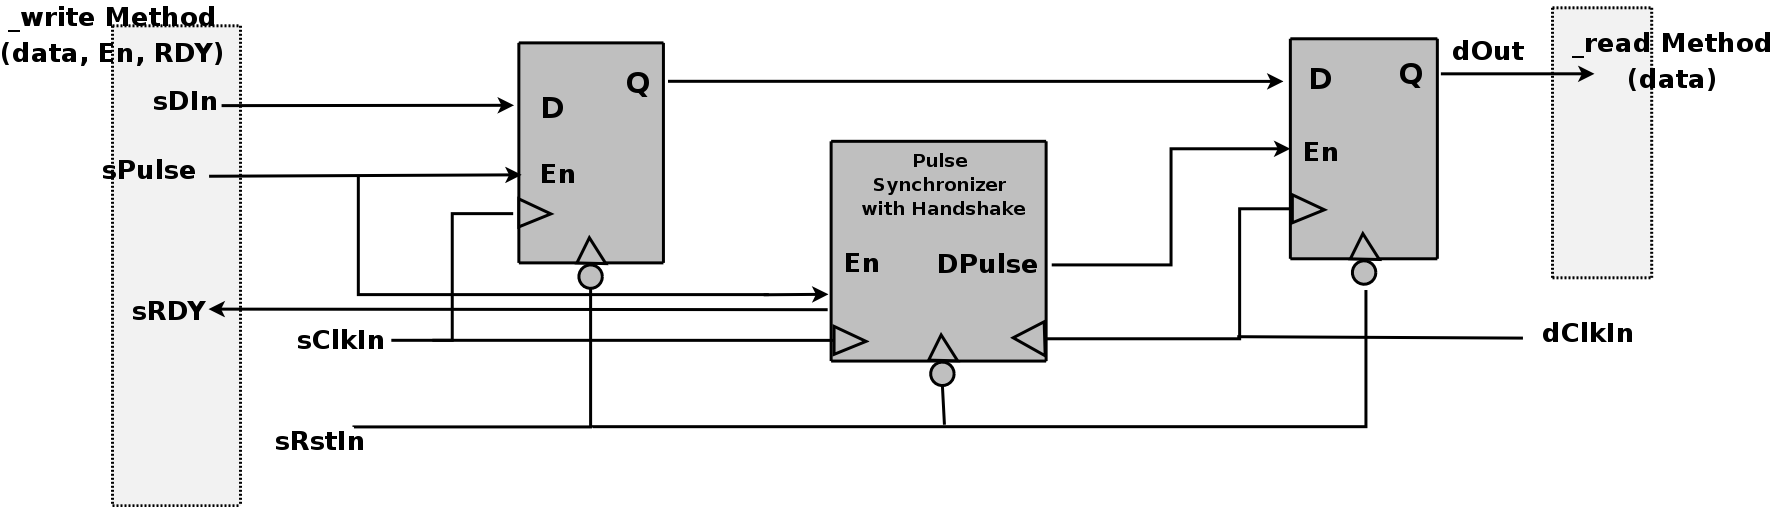
\includegraphics[height = 1.5 in]{LibFig/syncregister}
\caption{Register Synchronization Module (see Figure
\ref{synchandshake} for the pulse synchronizer with handshake)}
\label{syncregister}
\end{center}
\end{figure}

\begin{center}
\begin{tabular}{|p{1.4 in}|p{4.2 in}|}
\hline
&\\
\te{mkSyncReg}&Provides word synchronization across clock domains.  The in and out clocks,
along with the input reset, are explicitly provided.  The default clock
and reset are ignored.   \\
\cline{2-2}
&\begin{libverbatim}
module mkSyncReg #( a_type initValue,
                    Clock sClkIn, Reset sRstIn,
                    Clock dClkIn ) 
                  ( Reg #(a_type) )
   provisos (Bits#(a_type, sa) ) ;
\end{libverbatim}     
\\
\hline
\end{tabular}
\end{center} 

\index[function]{Clocks!mkSyncRegFromCC}
\index{mkSyncRegFromCC@\te{mkSyncRegFromCC} (module)}      
\begin{center}
\begin{tabular}{|p{1.4 in}|p{4.2 in}|}
\hline
&\\
\te{mkSyncRegFromCC}& Provides word synchronization from the current
clock domain.  The input clock and reset are the
current clock and reset.\\
\cline{2-2}
&\begin{libverbatim}
module mkSyncRegFromCC #( a_type initValue, 
                          Clock dClkIn )
                        ( Reg #(a_type) )
   provisos (Bits#(a_type, sa)) ; 
\end{libverbatim}     
\\
\hline
\end{tabular}
\end{center} 

\index[function]{Clocks!mkSyncRegToCC}
\index{mkSyncRegToCC@\te{mkSyncRegToCC} (module)}
\begin{center}
\begin{tabular}{|p{1.4 in}|p{4.2 in}|}
\hline
&\\
\te{mkSyncRegToCC}&Provides word synchronization to the current clock
domain. The
output clock is the current clock. The current reset is ignored.  \\
\cline{2-2}
&\begin{libverbatim}
module mkSyncRegToCC #( a_type initValue,
                        Clock sClkIn, Reset sRstIn )
                      ( Reg #(a_type) )
   provisos (Bits#(a_type, sa)) ;
\end{libverbatim}     
\\
\hline
\end{tabular}
\end{center} 

{\bf Verilog Modules}

The {\BSV} modules correspond to the following {\V}
modules, which are found in the BSC {\V} library, \te{\$BLUESPECDIR/Verilog/}.


\begin{center}
\begin{tabular}{|p {2.8 in}|p{2.8 in}|}
\hline
&\\
BSV Module Name & Verilog Module Name  \\
&\\
\hline
\hline
\te{mkSyncReg}&\te{SyncRegister.v}\\
\te{mkSyncRegFromCC}&\\
\te{mkSyncRegToCC}&\\
\hline
\end{tabular}
\end{center}
%===================================================================
\subsubsection{FIFO Synchronizers}

\index{SyncFIFOIfc@\te{SyncFIFOIfc} (interface)}
\label{syncfifoifc}

{\bf Description}

The \te{SyncFIFO} modules use FIFOs to synchronize data being sent
across clock domains, providing registered
full and empty signals (\te{notFull} and \te{notEmpty}). %  The
% \te{SyncFIFOFull} modules allow the user to choose whether or not the
% full and empty signals are registered.
Additional FIFO synchronizers,
\te{SyncFIFOLevel} and \te{SyncFIFOCount} can be found in the
\te{FIFOLevel} package (Section \ref{FIFOLevel}).  

{\bf Interfaces and Methods}

The \te{SyncFIFOIfc} interface defines an interface similar to the FIFOF
interface, except it does not have a \te{clear} method.

\begin{center}
\begin{tabular}{|p{.5in}|p{.7in}|p{1.8 in}|p{.6in}|p{1.2 in}|}
\hline
\multicolumn{5}{|c|}{\te{SyncFIFOIfc} Interface}\\
\hline
\multicolumn{3}{|c|}{Method}&\multicolumn{2}{|c|}{Arguments}\\
\hline
Name & Type & Description& Name &\multicolumn{1}{|c|}{Description} \\
\hline
\hline 
\te{enq}&\te{Action}&Adds an entry to the FIFO &\te{sendData}&Data
to be added\\
\hline
\te{deq}&\te{Action}&Removes the first entry from the FIFO&&\\
\hline
\te{first}&\te{a\_type}&Returns the first entry&&\\
\hline
\te{notFull}&\te{Bool}&Returns True if there is space and you can
\te{enq} into the FIFO &&\\
\hline
\te{notEmpty}&\te{Bool}&Returns True if there are elements in the FIFO
and you can \te{deq} from the FIFO&&\\
\hline
\end{tabular}
\end{center}

\begin{libverbatim}
     interface SyncFIFOIfc #(type a_type) ;
        method Action enq ( a_type sendData ) ;
        method Action deq () ;
        method a_type first () ; 
        method Bool notFull () ;
        method Bool notEmpty () ;
     endinterface
\end{libverbatim}


{\bf Modules}

\begin{figure}[ht]
\begin{center}
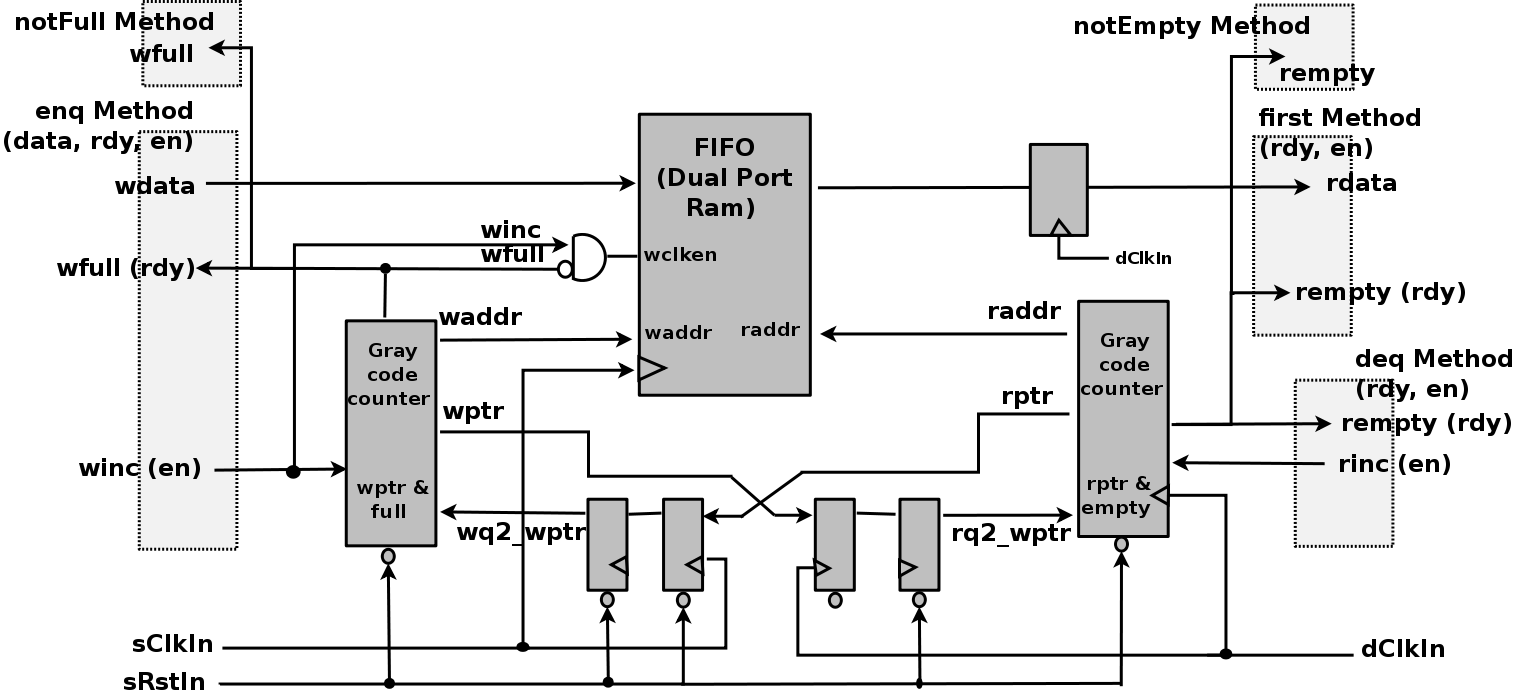
\includegraphics[width  = 5.5 in]{LibFig/syncfifo}
\caption{Synchronization FIFOs}
\label{syncfifo}
\end{center}
\end{figure}

\index[function]{Clocks!mkSyncFIFO}
\index{mkSyncFIFO@\te{mkSyncFIFO} (module)}
The \te{mkSyncFIFO}, \te{mkSyncFIFOFromCC} and \te{mkSyncFIFOToCC} modules
provide FIFOs for sending data across clock domains.  Data items
enqueued on the source side will arrive at the destination side and
remain  there until they are dequeued.  The depth of the FIFO is
specified by the \te{depth} parameter.  The full and empty signals are
registered.  The module \te{mkSyncFIFO1} is a 1 element synchronized FIFO.


\begin{center}
\begin{tabular}{|p{1.4 in}|p{4.2 in}|}
\hline
&\\
\te{mkSyncFIFO}&Provides a FIFO for sending data across clock domains.
 The \te{enq} method is in the source (\te{sClkIn}) domain, while the
 \te{deq}  and
 \te{first} methods are in the destination (\te{dClkIn}) domain.  The in and out clocks,
along with the input reset, are explicitly provided.  The default clock
and reset are ignored. \\
\cline{2-2}
&\begin{libverbatim}
module mkSyncFIFO #( Integer depth,
                     Clock sClkIn, Reset sRstIn,
                     Clock dClkIn )
                   ( SyncFIFOIfc #(a_type) )
   provisos (Bits#(a_type, sa));
\end{libverbatim}     
\\
\hline
\end{tabular}
\end{center} 
      
\index[function]{Clocks!mkSyncFIFOFromCC}
\index{mkSyncFIFOFromCC@\te{mkSyncFIFOFromCC} (module)}
\begin{center}
\begin{tabular}{|p{1.4 in}|p{4.2 in}|}
\hline
&\\
\te{mkSyncFIFOFromCC}&Provides a  FIFO to send data from the
current clock domain into a second clock domain. The input clock and reset are the
current clock and reset.\\
\cline{2-2}
&\begin{libverbatim}
module mkSyncFIFOFromCC #( Integer depth,
                           Clock dClkIn )
                         ( SyncFIFOIfc #(a_type) )
   provisos (Bits#(a_type, sa));
\end{libverbatim}     
\\
\hline
\end{tabular}
\end{center} 

\index[function]{Clocks!mkSyncFIFOToCC}
\index{mkSyncFIFOToCC@\te{mkSyncFIFOToCC} (module)}
\begin{center}
\begin{tabular}{|p{1.4 in}|p{4.2 in}|}
\hline
&\\
\te{mkSyncFIFOToCC}&Provides a  FIFO to send data from a
second clock domain into the current clock domain. The
output clock is the current clock. The current reset is ignored.   \\
\cline{2-2}
&\begin{libverbatim}
module mkSyncFIFOToCC #( Integer depth,
                         Clock sClkIn, Reset sRstIn )
                       ( SyncFIFOIfc #(a_type) )
   provisos (Bits#(a_type, sa));
\end{libverbatim}     
\\
\hline
\end{tabular}
\end{center} 

\index[function]{Clocks!mkSyncFIFO1}
\index{mkSyncFIFO1@\te{mkSyncFIFO1} (module)}

\begin{center}
\begin{tabular}{|p{1.4 in}|p{4.2 in}|}
\hline
&\\
\te{mkSyncFIFO1}&Provides a 1 element FIFO for sending data across
clock domains.  The 1 element module does not have a dedicated output
register and registers for full and empty, as in the depth > 1 module.
This module should be used in clock crossing applications where
complete FIFO handshaking is required, but data throughput or storage
is minimal.   \\
\cline{2-2}
&\begin{libverbatim}
module mkSyncFIFO #( Clock sClkIn, Reset sRstIn,
                     Clock dClkIn )
                   ( SyncFIFOIfc #(a_type) )
   provisos (Bits#(a_type, sa));
\end{libverbatim}     
\\
\hline
\end{tabular}
\end{center} 




%The following syncfifos were deprecated 12/21/10

% The sync FIFOFull modules are a variation of the Sync FIFO which allow
% the user to choose if the empty and full 
% signals are registered.  Registering the signals can give better
% synthesis results, since a comparator is removed from the empty or
% full path.  However, there is an additional cycle of latency
% before the empty or full signal is visible.
% \index[function]{Clocks!mkSyncFIFOFull}
% \index{mkSyncFIFOFull@\te{mkSyncFIFOFull} (module)}
% \begin{center}
% \begin{tabular}{|p{1.4 in}|p{4.2 in}|}
% \hline
% &\\
% \te{mkSyncFIFOFull}&Provides a registered FIFO for sending data across
% clock domains.  The in and out clocks,
% along with the input reset, are explicitly provided.  The default clock
% and reset are ignored. \\
% \cline{2-2}
% &\begin{libverbatim}
% module mkSyncFIFOFull #( Integer depth,  
%                          Bool regEmpty, 
%                          Bool regFull,
%                          Clock sClkIn, Reset sRstIn,
%                          Clock dClkIn )
%                        ( SyncFIFOIfc #(a_type) )
%    provisos (Bits#(a_type, sa));
% \end{libverbatim}     
% \\
% \hline
% \end{tabular}
% \end{center} 

% \index[function]{Clocks!mkSyncFIFOFromCCFull}
% \index{mkSyncFIFOFromCCFull@\te{mkSyncFIFOFromCCFull} (module)}
% \begin{center}
% \begin{tabular}{|p{1.4 in}|p{4.2 in}|}
% \hline
% &\\
% \te{mkSyncFIFOFromCCFull}&Provides a registered FIFO to send data from the
% current clock domain into a second clock domain.  The input clock and reset are the
% current clock and reset. \\
% \cline{2-2}
% &\begin{libverbatim}
% module mkSyncFIFOFromCCFull #( Integer depth, 
%                                Bool regEmpty, 
%                                Bool regFull,
%                                Clock dClkIn )
%                              ( SyncFIFOIfc #(a_type) )
%    provisos (Bits#(a_type, sa));
% \end{libverbatim}     
% \\
% \hline
% \end{tabular}
% \end{center} 

% \index[function]{Clocks!mkSyncFIFOToCCFull}
% \index{mkSyncFIFOToCCFull@\te{mkSyncFIFOToCCFull} (module)}
% \begin{center}
% \begin{tabular}{|p{1.4 in}|p{4.2 in}|}
% \hline
% &\\
% \te{mkSyncFIFOToCCFull}&Provides a registered FIFO to send data from a
% second clock domain into the current clock domain. The
% output clock is the current clock. The current reset is ignored.  \\
% \cline{2-2}
% &\begin{libverbatim}
% module mkSyncFIFOToCCFull #( Integer depth, 
%                              Bool regEmpty, 
%                              Bool regFull,
%                              Clock sClkIn, Reset sRstIn )
%                            ( SyncFIFOIfc #(a_type) )
%    provisos (Bits#(a_type, sa));
% \end{libverbatim}     
% \\
% \hline
% \end{tabular}
% \end{center} 

{\bf Verilog Modules}

The {\BSV} modules correspond to the following {\V}
modules, which are found in the BSC {\V} library, \te{\$BLUESPECDIR/Verilog/}.


\begin{center}
\begin{tabular}{|p {2.8 in}|p{2.8 in}|}
\hline
&\\
BSV Module Name & Verilog Module Name  \\
&\\
\hline
\hline
\te{mkSyncFIFO}&\te{SyncFIFO.v}\\
\te{mkSyncFIFOFromCC}&\\
\te{mkSyncFIFOToCC}&\\
\hline
\te{mkSyncFIFO1}&\te{SyncFIFO1.v}\\
% \te{mkSyncFIFOFull}&\\
% \te{mkSyncFIFOFromCCFull}&\\
% \te{mkSyncFIFOToCCFull}&\\
\hline
\end{tabular}
\end{center}
%====================================================================
\subsubsection{Asynchronous RAMs}
\index{DualPortRamIfc@\te{DualPortRamIfc} (interface)}
\index{mkDualRam@\te{mkDualRam} (module)}
\index[function]{Clocks!mkDualRam}

{\bf Description}

An asynchronous RAM provides a domain crossing by having its read and
write methods in separate clock domains.

{\bf Interfaces and Methods}

\begin{center}
\begin{tabular}{|p{.5in}|p{.5in}|p{1.6 in}|p{.5in}|p{1.7 in}|}
\hline
\multicolumn{5}{|c|}{\te{DualPortRamIfc} Interface}\\
\hline
\multicolumn{3}{|c|}{Method}&\multicolumn{2}{|c|}{Arguments}\\
\hline
Name & Type & Description& Name &\multicolumn{1}{|c|}{Description} \\
\hline
\hline 
\te{write}&\te{Action}&Writes data to a an address in a
RAM&\te{wr\_addr}&Address of datatype \te{addr\_t}\\
& &&\te{din}&Data of datatype \te{data\_t}\\
\hline
\te{read}&\te{data\_d}&Reads the data from the
RAM&\te{rd\_addr}&Address to be read from\\
\hline
\end{tabular}
\end{center}

\begin{libverbatim}
     interface DualPortRamIfc #(type addr_t, type data_t);
        method Action      write( addr_t wr_addr, data_t  din );
        method data_t      read ( addr_t rd_addr);
     endinterface: DualPortRamIfc
\end{libverbatim}


\begin{figure}[ht]
\begin{center}
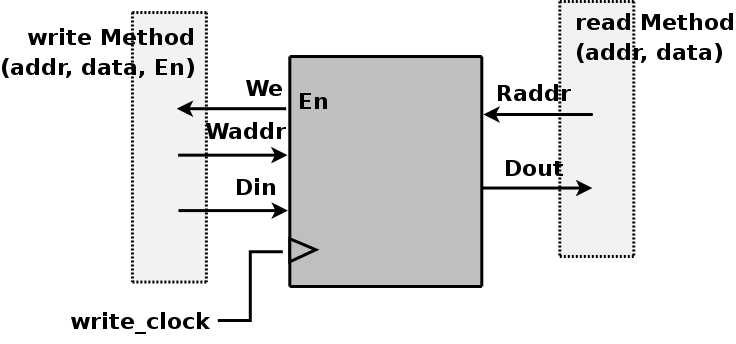
\includegraphics[height = 1.2 in]{LibFig/dualram}
\caption{Ansynchronous RAM}
\label{dualram}
\end{center}
\end{figure}


\begin{center}
\begin{tabular}{|p{1.4 in}|p{4.2 in}|}
\hline
&\\
\te{mkDualRam}&Provides an asynchronous RAM for  when the read and the
write  methods are in separate
clock domains.  The write method is clocked by the default clock, the
read method is not clocked.\\
\cline{2-2}
&\begin{libverbatim}
module mkDualRam( DualPortRamIfc #(addr_t, data_t) )
   provisos ( Bits#(addr_t, sa),
              Bits#(data_t, da) ) ;
\end{libverbatim}     
\\
\hline
\end{tabular}
\end{center} 

{\bf Verilog Modules}

The {\BSV} modules correspond to the following {\V}
modules, which are found in the BSC {\V} library, \te{\$BLUESPECDIR/Verilog/}.


\begin{center}
\begin{tabular}{|p {2.8 in}|p{2.8 in}|}
\hline
&\\
BSV Module Name & Verilog Module Name  \\
&\\
\hline
\hline
\te{mkDualRam}&\te{DualPortRam.v}\\
\hline
\end{tabular}
\end{center}
%=======================================================================
\subsubsection{Null Crossing Primitives}
%\index{ReadOnly@\te{ReadOnly} (interface)}

{\bf Description}

In these primitives, no synchronization is actually done.    It is up to
the  designer to verify that it is safe for the signal to be used in
the other domain. The \te{mkNullCrossingWire} is a wire synchronizer.
The \te{mkNullCrossingReg} modules are equivalent to a register
(\te{mkReg}, \te{mkRegA}, or \te{mkRegU} depending on the module)
followed by a \te{mkNullCrossingWire}.  

The older \te{mkNullCrossing} primitive is deprecated.

{\bf Interfaces} 

The \te{mkNullCrossingWire} module, shown in Figure \ref{syncwire},
provides the \te{ReadOnly} interface which is defined in the Prelude
library \ref{readonly}.

The \te{mkNullCrossingReg} modules provide the \te{CrossingReg}
interface.

{\bf Interfaces and Methods}

\begin{center}
\begin{tabular}{|p{.5in}|p{.5in}|p{1.6 in}|p{.5in}|p{1.7 in}|}
\hline
\multicolumn{5}{|c|}{\te{CrossingReg} Interface}\\
\hline
\multicolumn{3}{|c|}{Method}&\multicolumn{2}{|c|}{Arguments}\\
\hline
Name & Type & Description& Name &\multicolumn{1}{|c|}{Description} \\
\hline
\hline 
\te{\_write}&Action&Writes a value \te{datain}&\te{datain}&Data to be
written.\\
\hline
\te{\_read}&\te{a\_type}&Returns the value of the register in the
source clock domain&&\\
\hline
\te{crossed}&\te{a\_type}&Returns the value of the register in the
destination clock domain&&\\
\hline
\end{tabular}
\end{center}

\begin{libverbatim}
interface CrossingReg #( type a_type ) ;
   method Action _write(a datain) ;
   method a_type _read() ;
   method a_type crossed() ;
endinterface
\end{libverbatim}



{\bf Modules}

\begin{figure}[htb]
\begin{center}
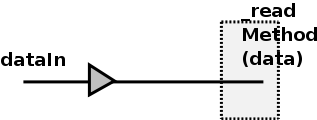
\includegraphics[height = .8 in]{LibFig/syncwire}
\caption{Wire synchronizer}
\label{syncwire}
\end{center}
\end{figure}


\index[function]{Clocks!mkNullCrossingWire}
\index{mkNullCrossingWire@\te{mkNullCrossingWire} (module)}
\begin{center}
\begin{tabular}{|p{1.4 in}|p{4.2 in}|}
\hline
&\\
\te{mkNullCrossingWire}&Defines a synchronizer that contains only a wire.
It is left up to the designer to ensure the clock crossing is safe.\\
\cline{2-2}
&\begin{libverbatim}
module mkNullCrossingWire #( Clock dClk, a_type dataIn )
                           ( ReadOnly#(a_type) )
   provisos (Bits#(a_type, sa)) ;
\end{libverbatim}     
\\
\hline
\end{tabular}
\end{center} 

\begin{figure}[htb]
\begin{center}
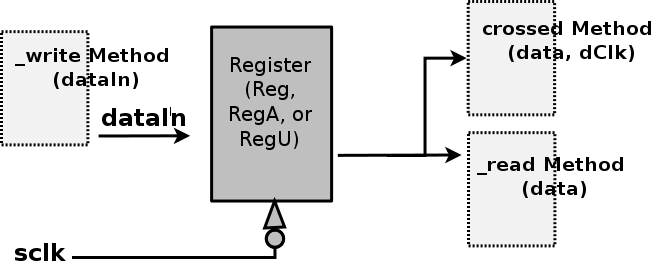
\includegraphics[height = 1.2 in]{LibFig/nullcrossingreg}
\caption{Register with wire synchronizer}
\label{nullcrossingreg}
\end{center}
\end{figure}

\index[function]{Clocks!mkNullCrossingReg}
\index{mkNullCrossingReg@\te{mkNullCrossingReg} (module)}
\begin{center}
\begin{tabular}{|p{1.4 in}|p{4.2 in}|}
\hline
&\\
\te{mkNullCrossingReg}&Defines a synchronizer that contains a register
with a synchronous reset value, 
followed by a wire synchronizer.
It is left up to the designer to ensure the clock crossing is safe.\\
\cline{2-2}
&\begin{libverbatim}
module mkNullCrossingReg( Clock dClk, a_type resetval, 
                          CrossingReg#(a_type) ifc )
   provisos (Bits#(a_type, sz_a)) ;
\end{libverbatim}     
\\
\hline
\end{tabular}
\end{center} 


\index[function]{Clocks!mkNullCrossingRegA}
\index{mkNullCrossingRegA@\te{mkNullCrossingRegA} (module)}
\begin{center}
\begin{tabular}{|p{1.4 in}|p{4.2 in}|}
\hline
&\\
\te{mkNullCrossingRegA}&Defines a synchronizer that contains a register
with a given reset value where reset is asynchronous, followed by a wire synchronizer.
It is left up to the designer to ensure the clock crossing is safe.\\
\cline{2-2}
&\begin{libverbatim}
module mkNullCrossingRegA( Clock dClk, a_type resetval, 
                          CrossingReg#(a_type) ifc )
   provisos (Bits#(a_type, sz_a)) ;
\end{libverbatim}     
\\
\hline
\end{tabular}
\end{center} 

\index[function]{Clocks!mkNullCrossingRegU}
\index{mkNullCrossingRegU@\te{mkNullCrossingRegU} (module)}
\begin{center}
\begin{tabular}{|p{1.4 in}|p{4.2 in}|}
\hline
&\\
\te{mkNullCrossingRegU}&Defines a synchronizer that contains a register
without a reset, followed by a wire synchronizer.
It is left up to the designer to ensure the clock crossing is safe.\\
\cline{2-2}
&\begin{libverbatim}
module mkNullCrossingRegU( Clock dClk, 
                           CrossingReg#(a_type) ifc )
   provisos (Bits#(a_type, sz_a)) ;
\end{libverbatim}     
\\
\hline
\end{tabular}
\end{center} 


{\bf Example: instantiating a null synchronizer }
\begin{libverbatim}
   // domain2sig is domain1sig synchronized to clk0 with just a wire.
   ReadOnly#(Bit#(2)) domain2sig <- mkNullCrossingWire (clk0, domain1sig);
\end{libverbatim}

Note: no synchronization is actually done.  This is purely a way to
tell BSC that it is safe to use the signal in the other
domain.  It is the responsibility of the designer to verify that this
is correct.

There are some restrictions on the use of a \te{mkNullCrossingWire}.
The expression used as the data argument must not have an implicit
condition, and there cannot be another rule which is required to 
schedule before any method called in the expression.

\te{mkNullCrossingWire}s may not be used in sequence to pass a signal
across multiple clock boundaries without synchronization.  Once a
signal has been crossed from one domain to a second domain without
synchronization, it cannot be subsequently passed unsynchronized to a
third domain (or back to the first domain).

{\bf Verilog Modules}

The {\BSV} modules correspond to the following {\V}
modules, which are found in the BSC {\V} library, \te{\$BLUESPECDIR/Verilog/}.

\begin{center}
\begin{tabular}{|p {2.8 in}|p{2.8 in}|}
\hline
&\\
BSV Module Name & Verilog Module Name  \\
&\\
\hline
\hline
\te{mkNullCrossingWire}&\te{BypassWire.v}\\
\hline
\end{tabular}
\end{center}
%===================================================================
% \subsubsection{Specialized Crossing Primitives}
% \label{crossing-prim}   
% \index{mkSynRegToSlow@\te{mkSyncRegToSlow} (module)}
% \index{mkSyncRegToFast@\te{mkSyncRegToFast} (module)}
% \index{mkSyncFIFOToSlow@\te{mkSyncFIFOToSlow} (module)}
% \index{mkSyncFIFOToFast@\te{mkSyncFIFOToFast} (module)}
% \index[function]{Clocks!mkSyncRegToSlow}
% \index[function]{Clocks!mkSyncRegToFast}
% \index[function]{Clocks!mkSyncFIFOToSlow}
% \index[function]{Clocks!mkSyncFIFOToFast}
% {\bf Description}




% The {\tt mkSyncRegToSlow} and {\tt mkSyncRegToFast} are specialized crossing primitives
% which can be used to transport data when clock edges are aligned,
% between the domains. The divided clocks and the appropriate
% interface needed for the module would typically be
% generated using the {\tt mkClockDivider} module (Section \ref{sec-clockdivider}).

% The crossing primitive is implemented via a single register,
% clocked by the slower (divided) clock.  For a fast  to slow crossing, the
% register  is only writable when the {\tt
% clockReady} bit of the divider interface is asserted.  This is an
% implicit  condition of the write method 
% module which prevents erroneous writes.  For a slow to fast
% crossing both the read and write methods are always available. 

% {\bf Modules}

% \begin{figure}[ht]
% \begin{center}
% 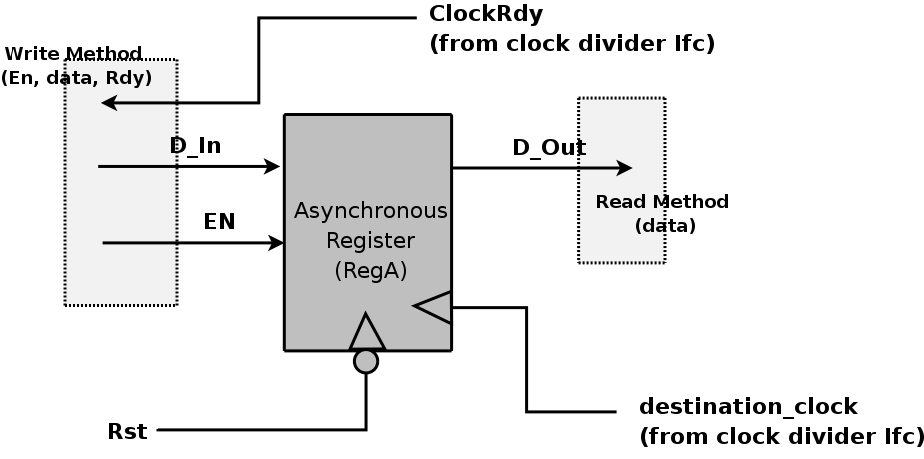
\includegraphics[height = 1.5 in]{LibFig/SyncRegSlow}
% \caption{Fast to Slow Crossing}
% \label{syncregslow}
% \end{center}
% \end{figure}


% \begin{center}
% \begin{tabular}{|p{1.4 in}|p{4.2 in}|}
% \hline
% &\\
% \te{mkSyncRegToSlow}&Provides a register to transport data when the
% clock edges are aligned between domains.  This module moves data from a
% fast to a slow domain.  The register is only writable when the {\tt
% clockReady} bit of the divider is asserted. \\
% \cline{2-2}
% &\begin{libverbatim}
% module mkSyncRegToSlow #( a_type initValue,
%                           ClockDividerIfc divider,
%                           Reset slowRstIn )
%                         ( Reg #(a_type) ) 
%    provisos (Bits#(a_type, sa)) ;
% \end{libverbatim}     
% \\
% \hline
% \end{tabular}
% \end{center} 
   
% \begin{figure}[ht]
% \begin{center}
% 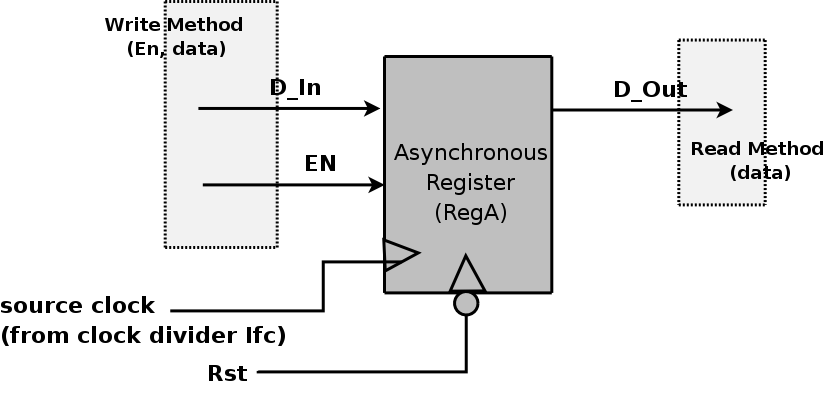
\includegraphics[height = 1.5 in]{LibFig/SyncRegtoFast}
% \caption{Slow to Fast Crossing}
% \label{syncregfast}
% \end{center}
% \end{figure}



% \begin{center}
% \begin{tabular}{|p{1.4 in}|p{4.2 in}|}
% \hline
% &\\
% \te{mkSyncRegToFast}&Provides a register to transport data when the
% clock edges are aligned between domains.  This module moves data from a
% slow to a fast domain.  The read and write methods are always available.  \\
% \cline{2-2}
% &\begin{libverbatim}
% module mkSyncRegToFast #( a_type initValue,
%                           ClockDividerIfc divider,
%                           Reset slowRstIn )
%                         ( Reg #(a_type) ) 
%    provisos (Bits#(a_type, sa)) ;
% \end{libverbatim}     
% \\
% \hline
% \end{tabular}
% \end{center} 
   
% The {\tt mkSyncFIFOToSlow} and {\tt mkSyncFIFOToFast} modules are  specialized crossing
% primitives which can be used to transport data when clock edges are
% aligned, between a fast clock domain and a slower clock domain. 
%  The derived clock and the
% \te{ClkNextRdy} signal would typically be
% generated using the {\tt mkClockDivider} module.  The synchronous
% FIFOs are clocked by the slower (divided) clock.  The \te{SyncFIFOIfc} is detailed
% in Section \ref{syncfifoifc}.

% \begin{figure}[ht]
% \begin{center}
% 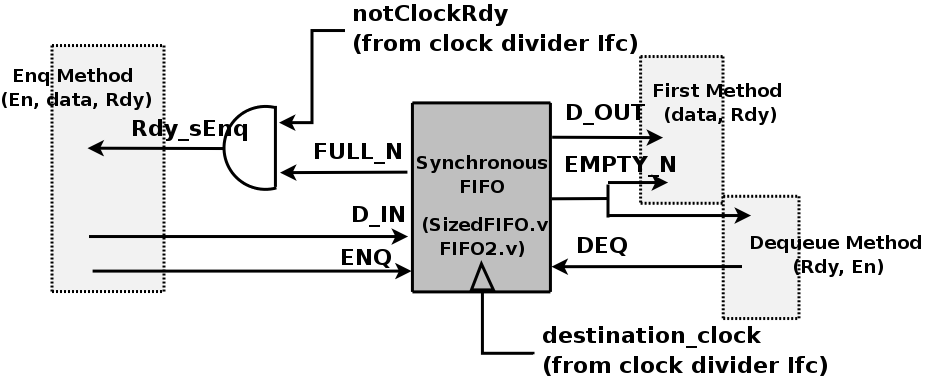
\includegraphics[height = 1.5 in]{LibFig/syncfifotoslow}
% \caption{Aligned clocks with FIFO - to slower domain}
% \label{fifotoslow}
% \end{center}
% \end{figure}


% \begin{center}
% \begin{tabular}{|p{1.4 in}|p{4.2 in}|}
% \hline
% &\\
% \te{mkSyncFIFOToSlow}&Provides a FIFO with specified depth to transport data from a fast clock domain
% to a slower clock domain when clock edges are aligned. The crossing primitive is implemented via a FIFO with the
% specified depth
% clocked by \te{dClkIn}. The FIFO is
% enqueued only when the {\tt syncBit} is asserted and the FIFO is not full. \\
% \cline{2-2}
% &\begin{libverbatim}
% module mkSyncFIFOToSlow #( Integer depth,
%                            ClockDividerIfc divider,
%                            Reset slowRstIn )
%                          ( SyncFIFOIfc #(a_type) ) 
%    provisos (Bits#(a_type, sa)) ;
% \end{libverbatim}     
% \\
% \hline
% \end{tabular}
% \end{center} 
      
% \begin{figure}[ht]
% \begin{center}
% 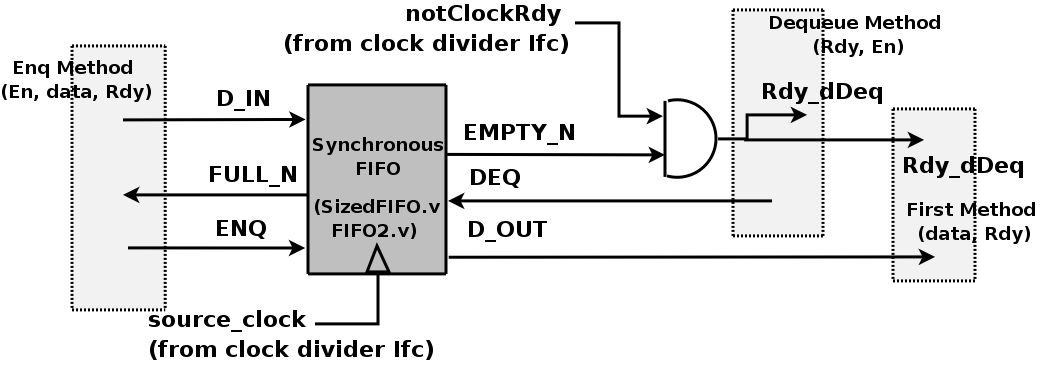
\includegraphics[height = 1.5 in]{LibFig/syncfifotofast}
% \caption{Aligned clocks with FIFO - to faster domain}
% \label{fifotofast}
% \end{center}
% \end{figure}


% \begin{center}
% \begin{tabular}{|p{1.4 in}|p{4.2 in}|}
% \hline
% &\\
% \te{mkSyncFIFOToFast}&Provides a FIFO with specified depth to
% transport data  from a slower clock domain
% to a faster clock domain when clock edges are aligned.  The crossing
% primitive  is implemented via a FIFO with the specified depth
% clocked by sClkIn (the source clock is the slower clock).
%  The FIFO is
% dequeued only when the {\tt syncBit} is asserted and the FIFO is not empty.   \\
% \cline{2-2}
% &\begin{libverbatim}
% module mkSyncFIFOToFast #( Integer depth,
%                            ClockDividerIfc divider,
%                            Reset slowRstIn )
%                          ( SyncFIFOIfc #(a_type) ) 
%    provisos (Bits#(a_type, sa)) ;
% \end{libverbatim}     
% \\
% \hline
% \end{tabular}
% \end{center} 

% {\bf Verilog Modules}

% The {\BSV} modules correspond to the following {\V}
% modules, which are found in the BSC {\V} library, \te{\$BLUESPECDIR/Verilog/}.

% \begin{center}
% \begin{tabular}{|p {2.8 in}|p{2.8 in}|}
% \hline
% &\\
% BSV Module Name & Verilog Module Name  \\
% &\\
% \hline
% \hline
% \te{mkSyncRegToSlow}&\te{RegA.v}\\
% \te{mkSyncRegToFast}&\\
% \hline
% \te{mkSyncFIFOToSlow}& \te{FIFO2.v}\\
% \te{mkSyncFIFOToFast}&\te{SizedFIFO.v}\\
% \hline
% \end{tabular}
% \end{center}
%===========================================================
\subsubsection{Reset Synchronization and Generation}



{\bf Description}

This section describes the interfaces and modules used to synchronize
reset signals from one clock domain to another and to 
create  reset signals.   Reset generation converts a Boolean type to a
Reset type, where the reset is associated with the default or
\te{clocked\_by} clock domain.


{\bf Interfaces and Methods}
\index{MakeResetIfc@\te{MakeResetIfc} (interface)}
\index{MuxRstIfc@\te{MuxRstIfc} (interface)}

The \te{MakeResetIfc} interface is provided by the reset generators
\te{mkReset} and \te{mkResetSync}.


\begin{center}
\begin{tabular}{|p{1 in}|p{1 in}|p{3 in}|}
\hline
\multicolumn{3}{|c|}{\te{MakeResetIfc} Interface}\\
\hline
\multicolumn{3}{|c|}{Method}\\
\hline
Name & Type & Description\\
\hline
\hline 
\te{assertReset}&\te{Action}&Method used to assert the reset\\
\hline
\te{isAsserted}&\te{Bool}&Indicates whether the reset is asserted\\
\hline
\te{new\_rst}&\te{Reset}&Generated output reset\\
\hline
\end{tabular}
\end{center}


\begin{libverbatim}
     interface MakeResetIfc;
        method Action assertReset();
        method Bool isAsserted();
        interface Reset new_rst;
     endinterface
\end{libverbatim}


The interface \te{MuxRstIfc} is provided by the \te{mkResetMux} module.

\begin{center}
\begin{tabular}{|p{.7in}|p{.7in}|p{1.5 in}|p{.4in}|p{1.5 in}|}
\hline
\multicolumn{5}{|c|}{\te{MuxRstIfc} Interface}\\
\hline
\multicolumn{3}{|c|}{Method}&\multicolumn{2}{|c|}{Arguments}\\
\hline
Name & Type & Description& Name &\multicolumn{1}{|c|}{Description} \\
\hline
\hline 
\te{select}&\te{Action}&Method used to select the reset based on the
Boolean value \te{ab}  &\te{ab}   &Value determines which input reset
to select\\
\hline
\te{reset\_out}&\te{Reset}&Generated output reset &&\\
\hline
\end{tabular}
\end{center}


\begin{libverbatim}
     interface MuxRstIfc;
        method Action select ( Bool ab );
        interface Reset reset_out;
     endinterface
\end{libverbatim}

{\bf Modules}
\index{mkSyncReset@\te{mkSyncReset} (module)}
\index{mkSyncResetFromCR@\te{mkSyncResetFromCR} (module)}
\index{mkAsyncReset@\te{mkAsyncReset} (module)}
\index{mkAsyncResetFromCR@\te{mkAsyncResetFromCR} (module)}
\index[function]{Clocks!mkSyncReset}
\index[function]{Clocks!mkSyncResetFromCR}
\index[function]{Clocks!mkAsyncReset}
\index[function]{Clocks!mkAsyncResetFromCR}


\paragraph{Reset Synchronization}

To synchronize resets from one clock domain to another, both
synchronous and asynchronous
modules are provided. 
The  {\tt stages} argument is the number of full clock cycles the
output reset is held for after the input reset is deasserted.  This
is shown as the number of flops in figures \ref{syncreseta} and \ref{syncreset}.
Specifying a 0 for the \te{stages} argument results in the creation of
a simple wire between \te{sRst} and \te{dRstOut}.

\begin{figure}[ht]
\begin{center}
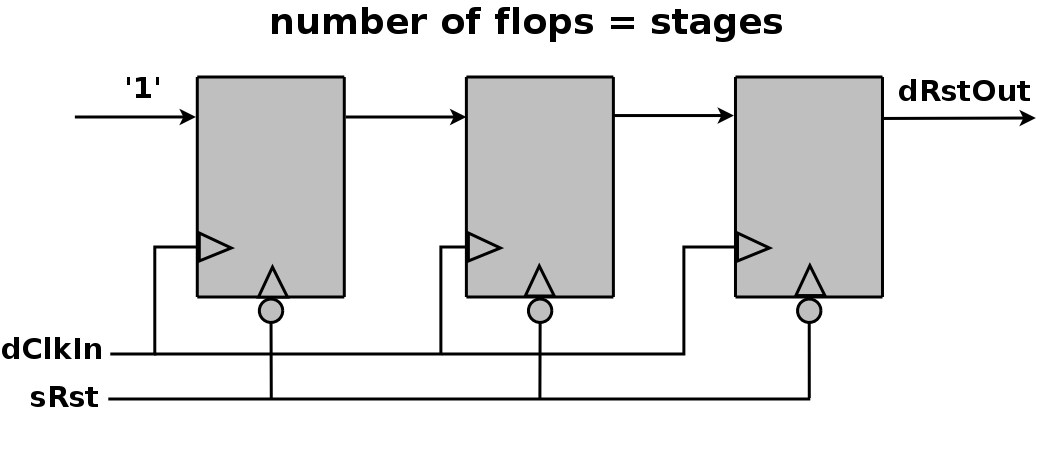
\includegraphics[height = 1.3 in]{LibFig/syncreseta}
\caption{Module for asynchronous resets}
\label{syncreseta}
\end{center}
\end{figure}


\begin{center}
\begin{tabular}{|p{1.4 in}|p{4.2 in}|}
\hline
&\\
\te{mkAsyncReset}&Provides synchronization of a source reset (\te{sRst})
to the destination  domain.  The  output reset occurs
immediately once the source reset is asserted.\\
\cline{2-2}
&\begin{libverbatim}
module mkAsyncReset #( Integer stages,
                       Reset sRst, 
                       Clock dClkIn ) 
                     ( Reset ) ;
\end{libverbatim}     
\\
\hline
\end{tabular}
\end{center} 

\begin{center}
\begin{tabular}{|p{1.4 in}|p{4.2 in}|}
\hline
&\\
\te{mkAsyncResetFromCR}&Provides synchronization of the
current reset to the destination domain.  There is no source reset \te{sRst}
argument because it is taken from the current reset.  The output reset
occurs immediately once the current reset is asserted.\\
\cline{2-2}
&\begin{libverbatim}
module mkAsyncResetFromCR #( Integer stages, 
                             Clock dClkIn )
                           ( Reset ) ;
\end{libverbatim}     
\\
\hline
\end{tabular}
\end{center} 


The less common {\tt mkSyncReset} modules are provided for
convenience, but these modules {\em require} that {\tt sRst} be held
during a positive edge of {\tt dClkIn} for the reset assertion to
be detected.  
Both \te{mkSyncReset} and \te{mkSyncResetFromCR} use the model in figure \ref{syncreset}.

\begin{figure}[ht]
\begin{center}
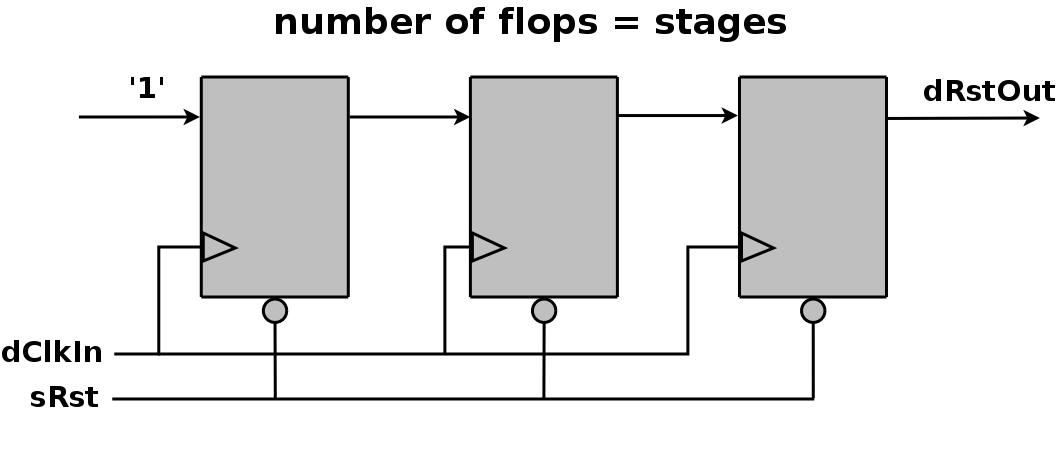
\includegraphics[height = 1.3 in]{LibFig/syncreset}
\caption{Module for synchronous resets}
\label{syncreset}
\end{center}
\end{figure}


\begin{center}
\begin{tabular}{|p{1.4 in}|p{4.2 in}|}
\hline
&\\
\te{mkSyncReset}& Provides synchronization of a source reset (\te{sRst})
to the destination  domain. 
The reset is asserted at the next rising edge of the clock.\\
\cline{2-2}
&\begin{libverbatim}
module mkSyncReset #( Integer stages 
                      Reset sRst, 
                      Clock dClkIn )
                    ( Reset ) ;
 
\end{libverbatim}     
\\
\hline
\end{tabular}
\end{center} 


\begin{center}
\begin{tabular}{|p{1.4 in}|p{4.2 in}|}
\hline
&\\
\te{mkSyncResetFromCR}&Provides synchronization of the
current reset to the destination domain.
The reset is asserted
at  the next rising edge of the clock.\\
\cline{2-2}
&\begin{libverbatim}
module mkSyncResetFromCR #( Integer stages 
                            Clock dClkIn ) 
                          ( Reset ) ;
\end{libverbatim}     
\\
\hline
\end{tabular}
\end{center} 






{\bf Example: instantiating a reset synchronizer }
\begin{libverbatim}
   // 2 is the number of stages
   Reset rstn2 <- mkAsyncResetFromCR (2, clk0);

   // if stages = 0, the default reset is used directly
   Reset rstn0 <- mkAsyncResetFromCR (0, clk0);
\end{libverbatim}

\paragraph{Reset Generation}

Two modules are provided for reset generation, {\tt  mkReset} and {\tt
mkResetSync}, where each module has one parameter, {\tt stages}.
The {\tt stages}  parameter is the number of full clock 
cycles the output reset is held after the \te{inRst}, as seen in
figure   \ref{makereseta},  is
deasserted.  Specifying a 0 for the {\tt stages} parameter results
in the creation of a simple wire between the input register and the
output reset.
 That is, the reset is asserted immediately and not held
after the input reset is deasserted.  It becomes the designer's
responsibility to ensure that the input reset is asserted for
sufficient time to allow the design to reset properly. 
The reset is controlled using the \te{assertReset} method of the
\te{MakeResetIfc} interface.
   
The difference between {\tt mkReset} and {\tt mkResetSync}
is that for the former, the assertion of reset is immediate, while
the later asserts reset at the next rising edge of the clock.
Note that use of 
\te{mkResetSync} is less common, since the reset requires clock edges
to take effect; failure to assert reset for a clock edge will 
result in a reset not being seen at the output reset.

\index{mkReset@\te{mkReset} (module)}
\index{mkResetSync@\te{mkResetSync} (module)}
\index{mkInitialReset@\te{mkInitialReset} (module)}
\index[function]{Clocks!mkReset}
\index[function]{Clocks!mkResetSync}
\index[function]{Clocks!mkInitialReset}


\begin{figure}[ht]
\begin{center}
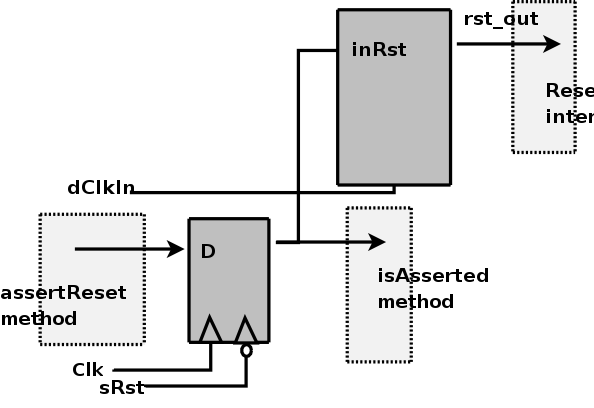
\includegraphics[height = 1.8 in]{LibFig/Makereseta}
\caption{Module for generating resets}
\label{makereseta}
\end{center}
\end{figure}


\begin{center}
\begin{tabular}{|p{1.4 in}|p{4.2 in}|}
\hline
&\\
\te{mkReset}&Provides conversion of a Boolean type to a Reset type,
where the reset is associated with  \te{dClkIn}.
This module uses the  model in figure \ref{makereseta}.
\te{startInRst} indicates the reset value of the register.  
If \te{startInRst} is True, the reset value of the register is 0, which
means the output reset will be asserted whenever the currentReset
(\te{sRst}) is asserted.  \te{rst\_out}  will remain asserted for the number of
clock cycles given by the stages parameter after \te{sRst} is
deasserted.  If \te{startInRst} is False, the output reset will not be
asserted when \te{sRst} is asserted, but only when the
\te{assert\_reset} method is invoked.  At the start of simulation
\te{rst\_out} will only be asserted if \te{startinRst} is True and
\te{sRst} is initially asserted.  \\
\cline{2-2}
&\begin{libverbatim}
module mkReset #( Integer stages,
                  Bool startInRst, 
                  Clock dClkIn )
                ( MakeResetIfc ) ;
\end{libverbatim}     
\\
\hline
\end{tabular}
\end{center} 


   
\begin{center}
\begin{tabular}{|p{1.4 in}|p{4.2 in}|}
\hline
&\\
\te{mkResetSync}& Provides conversion of a Boolean type to a Reset type,
where the reset is associated with  \te{dClkIn}
and the assertion of reset is at the next rising edge of the
clock. This module  uses the  model in figure
\ref{makereseta}.
\te{startInRst} indicates the reset value of the register.  
If \te{startInRst} is True, the reset value of the register is 0, which
means the output reset will be asserted whenever the currentReset
(\te{sRst}) is asserted.  \te{rst\_out}  will remain asserted for the number of
clock cycles given by the stages parameter after \te{sRst} is
deasserted.  If \te{startInRst} is False, the output reset will not be
asserted when \te{sRst} is asserted, but only when the
\te{assert\_reset} method is invoked.  At the start of simulation
\te{rst\_out} will only be asserted if \te{startinRst} is True and
\te{sRst} is initially asserted.  \\
\cline{2-2}
&\begin{libverbatim}
module mkResetSync #( Integer stages,
                      Bool startInRst,
                      Clock dClkIn )
                    ( MakeResetIfc ) ;
\end{libverbatim}     
\\
\hline
\end{tabular}
\end{center} 


\index[function]{Clocks!mkResetMux}
\index{mkResetMux@\te{mkResetMux} (module)}   
  A reset multiplexor {\tt mkResetMux}, as seen in figure
 \ref{resetmux}, 
 creates one reset signal by selecting between two existing reset
signals.  

\begin{figure}[ht]
\begin{center}
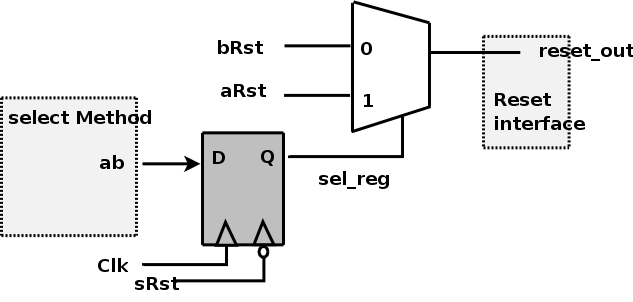
\includegraphics[height=1.4 in]{LibFig/resetmux}
\caption{Reset Multiplexor}
\label{resetmux}
\end{center}
\end{figure}


\begin{center}
\begin{tabular}{|p{1.4 in}|p{4.2 in}|}
\hline
&\\
\te{mkResetMux}& Multiplexor which selects between two input resets,
\te{aRst} and \te{bRst}, to create a single output
reset \te{rst\_out}.  The reset is selected through a Boolean value
provided to the \te{select} method 
where True selects \te{aRst}.\\
\cline{2-2}
&\begin{libverbatim}
module mkResetMux #( Reset aRst, Reset bRst )
                   ( MuxRstIfc rst_out ) ;
\end{libverbatim}     
\\
\hline
\end{tabular}
\end{center} 


For testbenches, in which an absolute clock is being created,
it is helpful to generate a reset for that clock.
The module {\tt mkInitialReset} is available for this purpose.  It
generates a reset which is asserted at the start of simulation.  
The reset is
asserted for  the  number of cycles
specified by  the parameter \te{cycles},  counting the start of time
as 1 cycle. Therefore, a \te{cycles} value of 1 will cause the reset to
turn off at the first clock tick.  
This module is not  synthesizable.   

\begin{center}
\begin{tabular}{|p{1.4 in}|p{4.2 in}|}
\hline
&\\
\te{mkInitialReset}&Generates a reset for \te{cycles} cycles, where
the  \te{cycles} parameter  must be
greater  than zero.  The \te{clocked\_by} clause indicates the clock
the reset is associated with.  This module is not synthesizable.  \\
\cline{2-2}
&\begin{libverbatim}
module mkInitialReset #( Integer cycles )
                       ( Reset ) ;
\end{libverbatim}     
\\
\hline
\end{tabular}
\end{center} 

Example:
\begin{verbatim}
    Clock c <- mkAbsoluteClock (10, 5);
    // a reset associated with clock c:
    Reset r <- mkInitialReset (2, clocked_by c);
\end{verbatim}

\index{mkResetEither@\te{mkResetEither} (module)}
\index[function]{Clocks!mkResetEither}
When two reset signals need to be combined so that some logic can be
reset when either input reset is asserted, the \te{mkResetEither}
module can be used.


\begin{figure}[ht]
\begin{center}
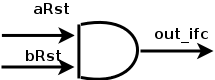
\includegraphics[height=.5 in]{LibFig/resetEither}
\caption{Reset Either}
\label{reseteither}
\end{center}
\end{figure}



\begin{center}
\begin{tabular}{|p{1.4 in}|p{4.2 in}|}
\hline
&\\
\te{mkResetEither}&Generates a reset which is asserted whenever either
input reset is asserted. \\
\cline{2-2}
&\begin{libverbatim}
module mkResetEither ( Reset aRst,
                       Reset bRst)
                     ( Reset out_ifc );
\end{libverbatim}
\\
\hline
\end{tabular}
\end{center} 

Example:
\begin{verbatim}
    Reset r <- mkResetEither(rst1, rst2);
\end{verbatim}

\index{mkResetInverter@\te{mkResetInverter} (module)}
\index[function]{Clocks!mkResetInverter}

\begin{center}
\begin{tabular}{|p{1.4 in}|p{4.2 in}|}
\hline
&\\
\te{mkResetInverter}&Generates an inverted Reset.\\
\cline{2-2}
&\begin{libverbatim}
module mkResetInverter#(Reset in)
                       (Reset);
\end{libverbatim}
\\
\hline
\end{tabular}
\end{center} 

\index{isResetAsserted@\te{isResetAsserted} (module)}
\index[function]{Clocks!isResetAsserted}

\begin{center}
\begin{tabular}{|p{1.4 in}|p{4.2 in}|}
\hline
&\\
\te{isResetAsserted}&Tests whether a Reset is asserted, providing a
Boolean value in the clock domain associated with the Reset.  \\
\cline{2-2}
&\begin{libverbatim}
module isResetAsserted( ReadOnly#(Bool) ifc ) ;
\end{libverbatim}
\\
\hline
\end{tabular}
\end{center} 



{\bf Verilog Modules}

The {\BSV} modules correspond to the following {\V}
modules, which are found in the BSC {\V} library, \te{\$BLUESPECDIR/Verilog/}.

\begin{center}
\begin{tabular}{|p {1.8 in}|p{1.8 in} |p{1.8in}|}
\hline
&&\\
BSV Module Name &Verilog Module Name&Comments  \\
&&\\
\hline
\hline
\te{mkASyncReset}&\te{SyncReset0.v}& when stages==0\\
\cline{2-3}
\te{mkASyncResetFromCR}&\te{SyncResetA.v}&\\
\hline
\te{mkSyncReset}&\te{SyncReset0.v}& when stages==0\\\cline{2-3}
\te{mkSyncResetFromCR}&\te{SyncReset.v}&\\
\hline
\te{mkReset}&\te{MakeReset0.v}&when stages==0\\\cline{2-3}
& \te{MakeResetA.v}&instantiates \te{SyncResetA} \\
\hline
\te{mkResetSync}&\te{MakeReset0.v}&when stages==0\\\cline{2-3}
&\te{MakeReset.v}&instantiates \te{SyncReset} \\
\hline
\te{mkResetMux}&\te{ResetMux.v}&\\
\hline
\te{mkResetEither}&\te{ResetEither.v}&\\
\hline
\te{mkResetInverter}&\te{ResetInverter.v}&\\
\hline
\te{isResetAsserted}&\te{ResetToBool.v}&\\
\hline
\end{tabular}
\end{center}















% ----------------

\subsection{Special Collections}

\subsubsection{ModuleContext}

\label{sec-ModuleContext}
\index{ModuleContext (package)}

{\bf Package}

\begin{verbatim}
import ModuleContext :: * ;
\end{verbatim}


{\bf Description}

An ordinary Bluespec module, when instantiated, adds  state
elements and rules to the growing accumulation of elements and rules
already in the design. 
In some designs,  items other than state 
elements and rules must be
accumulated as well. While there is a need to add these items, it is
also desirable to keep these additional design details separate from
the main design, keeping the natural structure of the design intact.

The \te{ModuleContext} package provides the capability of 
accumulating items and maintaining the compile-time state of
additional items, in such a way that it doesn't change the structure
of the original design.

The \te{ModuleContext} mechanism allows the designer to {\em hide} the
details of the additional interfaces.   Before the module can be
synthesized, it must be converted (or {\em exposed}) into a module containing
 only rules and state elements, as the
compiler does not know how to handle the other items.   The
\te{ModuleContext} package provides the mechanisms to allow additional
items to be collected, processed, and exposed.



{\bf Types and Type Classes}

The default BSV module type is \te{Module}, but you can define other
BSV module types as well.  The \te{ModuleContext} type is a variation
on the \te{Module} type that allows additional items, other than
states and rules, to be collected while elaborating the module
structure.   


The \te{ModuleContext} package defines the typeclass \te{Context},
which includes functions \te{getContext} and \te{putContext}.   A
\te{Context} typeclass has two type parameters: a module type
(\te{mc1}) and  the context (\te{c2}). 


\begin{verbatim}
   typeclass Context#(type mc1, type c2);
      module [mc1] getContext(c2) provisos (IsModule#(mc1, a));
      module [mc1] putContext#(c2 s)(Empty) provisos (IsModule#(mc1, a));
   endtypeclass
\end{verbatim}

A regular module type (\te{Module}) will have a context of \te{void}:
\begin{verbatim}
   instance Context#(Module, void);
\end{verbatim}

A module type of \te{ModuleContext} will return the context of the module:
\begin{verbatim}
   instance Context#(ModuleContext#(st1), st1);
\end{verbatim}

An instance is defined where the context type \te{st1} of the
\te{ModuleContext} and the context type \te{st2} are different, but \te{Gettable} (as defined in
\te{Hlist} Section \ref{sec-HList}):

\begin{verbatim}
   instance Context#(ModuleContext#(st1), st2)
      provisos (Gettable#(st1, st2));
\end{verbatim}


The modules \te{applyToContext} and \te{applyToContextM} are used to
apply a function over a  context.  The \te{applyToContextM} modules is
used for monadic functions.  

\index{applyToContext@\te{applyToContext} (module)}
\index[function]{ModuleContext!applyToContext}

\begin{tabular}{|p{1.1 in}|p{4.5 in}|}
\hline
& \\
\te{applyToContext} &Applies a function over a context.\\
\cline{2-2}
& \begin{libverbatim}
module [mc1] applyToContext#(function c2 f(c2 c))(Empty)
   provisos (IsModule#(mc1, a), Context#(mc1, c2));
\end{libverbatim}

\\
\hline
\end{tabular}

\index{applyToContextM@\te{applyToContextM} (module)}
\index[function]{ModuleContext!applyToContextM}

\begin{tabular}{|p{1.1 in}|p{4.5 in}|}
\hline
& \\
\te{applyToContextM} &Applies a monadic function over a context.\\
\cline{2-2}
& \begin{libverbatim}
module [mc1] applyToContextM#(function module#(c2) m(c2 c))
                             (Empty)
   provisos (IsModule#(mc1, a), Context#(mc1, c2));
\end{libverbatim}

\\
\hline
\end{tabular}


{\bf ClockContext}

The structure \te{ClockContext} is defined to be comprised of two
clocks: \te{clk1} and \te{clk2} and two resets: \te{rst1} and
\te{rst2}.

\begin{verbatim}
   typedef struct {
                   Clock clk1;
                   Clock clk2;
                   Reset rst1;
                   Reset rst2;
                  } ClockContext;
\end{verbatim}

An \te{initClockContext} is defined with the values of both clocks set to
\te{noClock} and both resets set to \te{noReset}:

\begin{verbatim}
   ClockContext initClockContext = ClockContext {
      clk1: noClock, clk2: noClock, rst1: noReset, rst2: noReset };
\end{verbatim}

{\bf Expose}

The \te{Expose} typeclass converts a context to an interface for a
synthesis boundary, converting it to a module type of \te{Module}.
The \te{Expose} typeclass provides the modules \te{unburyContext} and
\te{unburyContextWithClocks}. 


\begin{verbatim}
   typeclass Expose#(type c, type ifc)
      dependencies (c determines ifc);
\end{verbatim}

 An \te{HList} of contexts is
convertible if its elements are, and results in a \te{Tuple} of subinterfaces.

\begin{verbatim}
   instance Expose#(HList1#(ct1), ifc1)
      provisos (Expose#(ct1,ifc1));
\end{verbatim}

\begin{verbatim}
   instance Expose#(HCons#(c1,c2), Tuple2#(ifc1,ifc2))
      provisos (Expose#(c1,ifc1), Expose#(c2,ifc2));
  
   instance Expose#(ClockContext, Empty);
\end{verbatim}

\index{unburyContext@\te{unburyContext} (module)}
\index[function]{ModuleContext!unburyContext}

The \te{unburyContext} module is for use at the top level of a module
to be separately synthesized.  It takes as an argument a module which
is to be instantiated in a particular context, and an initial state
for that context.  The module is instantiated, and the final context
converted into an extra interface, returned in pair with the
intantiated module's own interface.

\begin{tabular}{|p{1.2 in}|p{4.6 in}|}
\hline
& \\
\te{unburyContext} &Converts a context to an interface for a synthesis
boundary.  An \te{HList} of contexts is convertible if its elements
are, and results in a tuple of subinterfaces.  \\
\cline{2-2}
& \begin{libverbatim}
module unburyContext#(c x)(ifc);

module unburyContext#(HList1#(ct1) c1)(ifc1);

module unburyContext#(HCons#(c1,c2) c12)(Tuple2#(ifc1,ifc2));

module unburyContext#(ClockContext x)();
\end{libverbatim}
\\
\hline
\end{tabular}

\index{unburyContextWithClocks@\te{unburyContextWithClocks} (module)}
\index[function]{ModuleContext!unburyContextWithClocks}

The \te{unburyContextWithClocks} takes a \te{ClockContext} along with
the \te{Context}  it is specifically handling

% The \te{unburyWithClocks}  module is a top-level module for use within
% a separately synthesized module. It takes two clocks and two resets as
% extra arguments, and embeds them in the \te{ClockContext} before
% supplying the \te{CompleteContext} to the argument module. 

\begin{tabular}{|p{1.6 in}|p{4.2 in}|}
\hline
&\\
\te{unburyContextWithClocks}& Converts a context to an interface for a
synthesis boundary and takes a ClockContext as a second argument.\\
\cline{2-2}
& \begin{libverbatim}
module unburyContextWithClocks#(c x, ClockContext cc)
                               (ifc);

module unburyContextWithClocks#(HList1#(ct1) c1, 
                                ClockContext cc)(ifc1);

module unburyContextWithClocks#(HCons#(c1,c2) c12, 
                                ClockContext cc)
                                (Tuple2#(ifc1,ifc2));

module unburyContextWithClocks#(ClockContext x, 
                                ClockContext cc)();
\end{libverbatim}
\\
\hline
\end{tabular}




{\bf Hide}

The \te{Hide} typeclass provides the module \te{reburyContext}, which
takes an interface as an argument (and provides an Empty interface).
It is intended to be run in a context which can absorb the information
from the interface.  As with \te{Expose}, a \te{Tuple} of interfaces
can be hidden if each element can be hidden.

\index{reburyContext@\te{reburyContext} (module)}
\index[function]{ModuleContext!reburyContext}


\begin{tabular}{|p{1.2 in}|p{4.6 in}|}
\hline
& \\
\te{reburyContext} &Connects the provided interface with the
surrounding context. \\
\cline{2-2}
& \begin{libverbatim}
   module [mc] reburyContext#(ifc i)(Empty);

   module [mc] reburyContext#(Empty i)(Empty);

   module [mc] reburyContext#(Tuple2#(ifc1,ifc2) i12)(Empty);
  
\end{libverbatim}
\\
\hline
\end{tabular}

{\bf ContextRun}

The \te{ContextRun} and \te{ContextsRun} typeclasses provides modules to run modules in
contexts.   The module \te{runWithContext}  runs a module with an
entirely new context.  % The modules 
% \te{runWithOneMoreContext} and \te{runWithMoreContexts} adds items
% onto a context.  In both cases, the module takes as an argument the
% initial state of the new part of the context, and the final version
% of the new part of the context is returned as the result of the run,
% and the old part of the context continues to accumulate.

\begin{verbatim}
typeclass ContextRun#(type m, type c1, type ctx2)
   dependencies ((m, c1) determines ctx2);
\end{verbatim}


\begin{verbatim}
typeclass ContextsRun#(type m, type c1, type ctx2)
   dependencies ((m, c1) determines ctx2);
\end{verbatim}


\index{runWithContext@\te{runWithContext} (function)}
\index[function]{ModuleContext!runWithContext}

\begin{tabular}{|p{1.2 in}|p{4.6 in}|}
\hline
& \\
\te{runWithContext} &Runs a module with an entirely new context.\\
\cline{2-2}
& \begin{libverbatim}
module [m] runWithContext #(c1 initState, 
                            ModuleContext#(ctx2, ifcType) mkI)
                           (Tuple2#(c1, ifcType));

module [ModuleContext#(ctx)] runWithContext#(c1 initState,
			     ModuleContext#(HCons#(c1, ctx), ifcType) mkI)
                            (Tuple2#(c1, ifcType));

module [Module] runWithContext#(c1 initState, 
                                ModuleContext#(c1,ifcType) mkI)
                               (Tuple2#(c1, ifcType));
\end{libverbatim}
\\
\hline
\end{tabular}

\index{runWithContexts@\te{runWithContexts} (function)}
\index[function]{ModuleContext!runWithContext}

\begin{tabular}{|p{1.2 in}|p{4.6 in}|}
\hline
& \\
\te{runWithContexts} &Runs a module with an entirely new context.\\
\cline{2-2}
& \begin{libverbatim}
module [m] runWithContexts#(c1 initState, 
                            ModuleContext#(ctx2, ifcType) mkI)
                           (Tuple2#(c1, ifcType));

module [ModuleContext#(ctx)] runWithContexts#(c1 initState,
			     ModuleContext#(ctx2, ifcType) mkI)
                            (Tuple2#(c1, ifcType));

module [Module] runWithContexts#(c1 initState, 
                                 ModuleContext#(c1, ifcType) mkI)
                                (Tuple2#(c1, ifcType));
\end{libverbatim}
\\
\hline
\end{tabular}




{\bf Contexts.defines}

BSC provides macros in the  \te{Context.defines} file to
handle the treatment of the module contexts at synthesis boundaries.

\begin{enumerate}
\item The designer defines a leaf or intermediate node module, with
module type \te{[ErrorReporter]} or \te{[ErrorReporterA]}, appending a
\te{0} to its name (e.g. \te{mkM0}).  Elsewhere in the package the
appropriate macro is chosen from the macros \te{SynthBoundary} and
\te{SynthBoundaryWithClocks}. 

\item The macro defines a synthesizable version of the module,
\te{mkMV}, which provides the original interface together with an
error-reporting subinterface.  It also defines a module with the
original name \te{mkM} to be used for instantiating the original
module.  It uses the Context mechanism to re-bury the error-reporting
plumbing and returns the original interface of the original \te{mkM)} module
\end{enumerate}

These macros assume that the complete module context (such as an
\te{HList} of individual contexts) is named \te{CompleteContext} and
that its initial value may be obtained from either
 \te{mkInitialCompleteContext} or \te{mkInitialCompleteContextWithClocks}.


{\bf Example Without Clocks}

\begin{verbatim}
SynthBoundary(mkM,IM)
\end{verbatim}

Becomes
\begin{verbatim}
(*synthesize*)
module [Module] mkMV(Tuple2#(CompleteContextIfc,IM));
   let init <- mkInitialCompleteContext;
   let _ifc <- unbury(init, mkM0);
   return _ifc;
endmodule

module [ModuleContext#(CompleteContext)] mkM(IM);
   let _ifc <- rebury(mkMV);
   return _ifc;
endmodule
\end{verbatim}
{\bf Example With Clocks}
\begin{verbatim}
SynthBoundaryWithClocks(mkM,IM)
\end{verbatim}
Becomes

\begin{verbatim}
(*synthesize*)
module [Module] mkMV#(Clock c1,Reset r1,Clock c2,Reset r2)(Tuple2#(CompleteContextIfc,IM));
   let init <- mkInitialCompleteContextWithClocks(c1, r1, c2, r2);
   let _ifc <- unburyWithClocks(initialCompleteContext, c1, r1, c2, r2, mkM0);
   return _ifc;
endmodule

module [ModuleContext#(CompleteContext)] mkM(IM);
   let _ifc <- reburyWithClocks(mkMV);
   return _ifc;
endmodule
\end{verbatim}


\subsubsection{ModuleCollect}

{\bf Package}
\index{ModuleCollect@\te{ModuleCollect} (package)}
\label{package-modulecollect}

\begin{verbatim}
import ModuleCollect :: * ;
\end{verbatim}


{\bf Description}

The \te{ModuleCollect} package provides the capability of adding
additional items, such as configuration bus connections, 
to a design in such a way that it does not change the 
structure of the design.  This section provides a brief overview of
the package.  
For a more detailed description of its usage, see the \te{CBus}
package (\ref{lib-cbus}), which utilizes  \te{ModuleCollect}.
There is also  a detailed  example and  more complete discussion of the \te{CBus}
package in the configbus tutorial in the BSV/tutorials directory.


An ordinary {\BS} module, when instantiated, adds its own state
elements and rules to
the growing accumulation of state elements and rules defined in the
design.  In some designs, for example a configuration bus, additional
items, such as the logic for the
 bus address decoding  must be accumulated as well. While there is a
need to add these items, it is also desirable to keep these
additional design details separate from the main design, keeping the
natural structure of the design intact.  

The \te{ModuleCollect} mechanism allows the designer to \emph{hide} the details of the
additional interfaces.    A module which is going to be synthesized must contain
only rules and state elements, as the compiler does not know how to
handle the additional items.  Therefore, the collection must be
brought into the open, or exposed, before the module can be
synthesized.  The \te{ModuleCollect} package 
provides the mechanisms to allow these additional
items to be collected, processed and exposed.

% An ordinary module, when
% instantiated, adds its own items to the growing accumation of 
% state  elements, and rules, which are processed by later stages of
% the compiler.  The
% \te{ModuleCollect} package allows other items to be accumulated too.  But
% this extra \emph{collection} must be exposed and processed at a higher
% level: in particular, any module which is to be synthesized must not
% be collecting any extra stuff, as the compiler would not know how to
% handle it.  The \te{ModuleCollect} package provides functions to
% create, process and expose collections.

{\bf Types and Type Classes}

The \te{ModuleCollect} type is a variation  on the \te{Module} type
that allows additional items, other than states and rules,  to be collected
while  elaborating the module structure.    A module defining the
accumulation of a special collection will have the type of
\te{ModuleCollect}  which is defined as a type of \te{ModuleContext}
(Section \ref{sec-ModuleContext}):  
\index{ModuleCollect@\te{ModuleCollect} (type)}

\begin{verbatim}
typedef ModuleContext#(HList1#(UAList#(a))) ModuleCollect#(type a_type);
\end{verbatim}


% \BBS
%  struct ModuleCollect#(a\_type, ifc) 
%        {\rm{\emph{$\cdots$ abstract $\cdots$}}}
% \EBS

where \te{a\_type}  defines the type of 
the items being collected.   The collection is kept as an
\te{HList},  therefore each item in the  collection does not  have the
same type.  % The 
% collection is  associated with \te{ifc}, the device module interface.

Your new type of module is a \te{ModuleCollect} defined to collect a
specific type.  It is often convenient to give a name to your new type
of module using the \te{typedef} keyword.

For example:
\begin{libverbatim}
     typedef ModuleCollect#(element_type, ifc_device)
             MyModuleType#(type ifc_device)
\end{libverbatim}

specifies a type named \te{MyModuleType}.

An ordinary module, one defined with the keyword \te{module} without
a type in square brackets immediately after it, can be of any module
type.  It is polymorphic, and when  instantiated  takes the
type of the surrounding module context.   Only modules of type
\te{Module} can be synthesized, so the  \te{*synthesize*}
attribute forces the type to be \te{Module}.  This is equivalent to
writing:
\begin{libverbatim}
    module [Module]...
\end{libverbatim}
Normally, all the modules instantiated inside a synthesized module take
the type \te{Module}.

A module which is accumulating a collection must have the appropriate
type, specified in square brackets immedately after the keyword, as
shown in the following example:
\begin{libverbatim}
    module [AssertModule] mkAssertionReg...
\end{libverbatim}
The complete example is found later in this section.
This implies that any module instantiating \te{mkAssertionReg} is no
longer polymorphic, its type is constrained by the inner module, so it
will have to be explicitly given the \te{AssertModule} type too. Note,
however, that you can continue to instantiate other modules not
concerned with the collection (for example, \te{mkReg}, \te{mkFIFO},
etc.) alongside \te{mkAssertReg} just as before.  But now they will
take the type \te{AssertModule} from the context instead of the type
\te{Module}.  

Since only modules of type \te{Module} can be synthesized, before this
group of \te{AssertModule} instantiations can be 
synthesized, you must use  \te{exposeCollection} to  contain
the collection in a top-level module of type \te{Module}. 


% An ordinary module, one not
% collecting anything other than rules and state
% elements has the type \te{Module}.  When no type is explicitly given,
% the compiler fixes it to \te{Module} when the module is synthesized.
% But for a module accumulating a
% collection, the type must be explicitly given, and it is supplied in
% square brackets immediately after the keyword \te{module}.  Because in
% our example above, 
% the new type alias only takes one argument, the interface, we can use
% it here without arguments:

% \begin{libverbatim}
%     module [MyModuleType] mkSubDesign#(x,y) (IfcType) ;
% \end{libverbatim}

% Since only modules of type \te{Module} can be synthesized 
%  the collection  be  exposed before synthesis, by applying the
%  function \te{exposeCollection}.  The module type of
% the function \te{exposeCollection} is \te{Module}, so once the
% collection has  been exposed 
%  the design is ready for synthesis. 



{\bf Interfaces}

The \texttt{IWithCollection} interface couples the normal module
interface (the \texttt{device} interface) with the collection of
collected items (the \texttt{collection} interface).  This is the
interface provided by the \te{exposeCollection} function.  It separates
the collection list and the device  module interface, to allow the module to be synthesized.

\begin{verbatim}
   interface IWithCollection #(type a, type i);
       method i device();
       method List#(a) collection();
   endinterface: IWithCollection
\end{verbatim}

OLD:
\begin{verbatim}
   interface IWithCollection #(type collection_type, type item_type);
      interface item_type device();
      interface List#(collection_type) collection();
   endinterface: IWithCollection
\end{verbatim}


{\bf Modules and Functions}

% There are three functions defined within the \te{ModuleCollect}
% package; \te{addToCollection}, \te{exposeCollection}, and
% \te{mapCollection}.

In the course of
evaluating a module body during its instantiation, an item
may be added to the current collection by using the function
\texttt{addToCollection}. \index{addToCollection@\te{addToCollection} (\te{ModuleCollect} function)}

\begin{center}
\begin{tabular}{|p{1.1 in}|p{4.5 in}|}
\hline
&  \\
\te{addToCollection}&Adds an item to the collection.\\
&  \\
\cline{2-2}
&\begin{libverbatim}
function ModuleCollect#(a_type, ifc) 
         addToCollection(a_type item); 
\end{libverbatim}
\\
\hline
\end{tabular}
\end{center}

Once a set of items has been collected, those items must be
exposed  before synthesis.  The \texttt{exposeCollection} module
constructor is used to bring the collection out into the open. 
The \texttt{exposeCollection} module  takes as an argument a
\texttt{ModuleCollect} module (\texttt{m}) with interface \texttt{ifc},
and provides an \texttt{IWithCollection} interface.  
\index{exposeCollection@\te{exposeCollection} (\te{ModuleCollect} function)}

\begin{tabular}{|p{1.1 in}|p{4.5 in}|}
\hline
&  \\
\te{exposeCollection}&Expose the collection to allow the module to be synthesized.\\
&\\
\cline{2-2}
&\begin{libverbatim}
module exposeCollection#(ModuleCollect#(a_type, ifc) m)
                        (IWithCollection#(a_type, ifc));
\end{libverbatim}
\\
\hline
\end{tabular}

Finally, the \texttt{ModuleCollect} package provides a function, 
\texttt{mapCollection}, to apply a function to each item in the
current collection.
\index{mapCollection@\te{mapCollection} (\te{ModuleCollect} function)}

\begin{tabular}{|p{1.1 in}|p{4.5 in}|}
\hline
&  \\
\te{mapCollection}&Apply a function to each item added to the collection within
the second argument.\\
&  \\
\cline{2-2}
&\begin{libverbatim}
function ModuleCollect#(a_type, ifc) 
   mapCollection(function a_type x1(a_type x1), 
                 ModuleCollect#(a_type, ifc) x2); 
\end{libverbatim}
\\
\hline
\end{tabular}

{\bf Example - Assertion Wires}
\begin{libverbatim}
// This example shows excerpts of a design which places various
// test conditions (Boolean expressions) at random places in a design,
// and lights an LED (setting an external wire to 1), if the condition
// is ever satisfied.

import ModuleCollect::*;
import List::*;
import Vector::*;
import Assert::*;

// The desired interface at the top level is:
interface AssertionWires#(type n);
   method Bit#(n) wires;
   method Action clear;
endinterface

// The "wires" method tells which conditions have been set, and the
// "clear" method resets them all to 0.  
// The items in our extra collection will be interfaces of the
// following type:

interface AssertionWire;
   method Integer index;   //Indicates which wire is to be set if
   method Bool fail;       // fail method ever returns true.
   method Action clear;
endinterface

// We next define the "AssertModule" type.  This is to behave like an
// ordinary module providing an interface of type "i", except that it
// also can collect items of type "AssertionWire":

typedef ModuleCollect#(AssertionWire, i) AssertModule#(type i);

typedef Tuple2#(AssertionWires#(n), i) AssertIfc#(type i, type n);

...

// The next definition shows how items are added to the collection.
// This is the module which will be instantiated at various places in
// the design, to test various conditions.  It takes one static
// parameter, "ix", to specify which wire is to carry this condition,
// and one dynamic parameter (one varying at run-time) "c", giving the
// value of the condition itself.  

interface AssertionReg;
   method Action set;
   method Action clear;
endinterface

module [AssertModule] mkAssertionReg#(Integer ix)(AssertionReg);

   Reg#(Bool) cond <- mkReg(False);

   // an item is defined and added to the collection
   let item = (interface AssertionWire;
                 method index;
                    return (ix);
                 endmethod
                 method fail;
                    return(cond);
                 endmethod
                 method Action clear;
                     cond <= False;
                 endmethod
               endinterface);
   addToCollection(item);
   ...
endmodule
                     
// the collection must be exposed before synthesis       
module [Module] exposeAssertionWires#(AssertModule#(i) mkI)(AssertIfc#(i, n));
   
   IWithCollection#(AssertionWire, i) ecs <- exposeCollection(mkI);
   
   ...(c_ifc is created from the list ecs.collection)

   // deliver the array of values in the registers
   let dut_ifc = ecs.device;
    
   // return the values in the collection, and the ifc of the device
   return(tuple2(c_ifc, dut_ifc));
endmodule
\end{libverbatim}


\subsubsection{CBus}
\index{CBus@\te{CBus} (package)}
\label{lib-cbus}

{\bf Package}

\begin{verbatim}
import CBus :: * ;
\end{verbatim}



{\bf Description}

The \te{CBus} package provides the interface, types and modules to
implement a configuration bus capability providing access to the
control and status registers in a given module hierarchy.  This
package  utilizes the
\te{ModuleCollect} package and functionality,  as described in section
\ref{package-modulecollect}.  The \te{ModuleCollect} package allows
items in addition to usual state elements and rules to be accumulated.
This is required to collect up the interfaces of the control status
registers included in a module and to add the associated logic and
ports required to allow them to be accessed via a configuration bus.

%For a more complete discussion of the \te{CBus}
%package, consult the configbus tutorial in the BSV/tutorials directory.



{\bf Types and Type Classes}

The type \te{CBusItem} defines the type of item to be collected by
\te{ModuleCollect}.   The items to be collected are the same as the
ifc which we will later expose, so we use a type alias:

\begin{libverbatim}
typedef CBus#(size_address, size_data) 
        CBusItem #(type size_address, type size_data);
\end{libverbatim}

The type \te{ModWithCBus} defines the type of module which is
collecting \te{CBusItem}s.  An ordinary module, one not collecting anything
other than state elements and rules, has the type \te{Module}.   Since
\te{CBusItem}s are
being collected, a  module type \te{ModWithCBus} is
defined.  When the module  type is not \te{Module}, 
the  type  must
be specified in square brackets immediately after the \te{module}
keyword in  the module definition. 

\begin{libverbatim}
typedef ModuleCollect#(CBusItem#(size_address, size_data), item) 
        ModWithCBus#(type size_address, type size_data, type item);
\end{libverbatim}



% typedef struct {
%    Bit#(size_address) a;
%    Bit#(size_address) o;
%    } CRAddr#(numeric type size_address) deriving(Bits, Eq);



{\bf Interface and Methods}
\index{CBus@\te{CBus} (interface)}
\index{IWithCBus@\te{IWithCBus} (interface)}

The \te{CBus} interface provides \te{read} and \te{write} methods to
access control status registers.  It is polymorphic in terms of the
size of the address bus (\te{size\_address}) and size of the data bus
(\te{size\_data}).  

%defines the interface for the configuration bus (the {\em back door} interface).  
\begin{center}  
\begin{tabular}{|p{.6 in}|p{4 in}|}
\hline
\multicolumn{2}{|c|}{\te{CBus} Interface}\\
\hline
Name &  Description\\
\hline
\hline 
&\\
\te{write}&Writes the \te{data} value to the register if and
only if the value of \te{addr} matches the address of the register.\\
\hline
&\\
\te{read}&Returns the value of the associated
register if and only if \te{addr} matches the register address.  In all
other cases the \te{read} method returns an \te{Invalid} value.\\
\hline
\end{tabular}
\end{center}


\begin{libverbatim}
interface CBus#(type size_address, type size_data);
   method Action write(Bit#(size_address) addr, Bit#(size_data) data);
   (* always_ready *)
   method ActionValue#(Bit#(size_data)) read(Bit#(size_address) addr);
endinterface

\end{libverbatim}

The \te{IWithCBus} interface combines the \te{CBus} interface with a
normal module interface.  It is defined as a structured
interface with two subinterfaces: \te{cbus\_ifc} (the associated
configuration bus interface) and \te{device\_ifc} (the associated
device interface).   It is polymorphic in terms of the type of the
configuation bus interface and the type of the device interface.  

%the device interface (the {\em front door} interface).

\begin{libverbatim}
interface IWithCBus#(type cbus_IFC, type device_IFC);
   interface cbus_IFC cbus_ifc;
   interface device_IFC device_ifc;
endinterface
\end{libverbatim}



{\bf Modules}

\index{collectCBusIFC@\te{collectCBusIFC} (module)}
\index[function]{CBus!collectCBusIFC}

The \te{collectCBusIFC} module 
takes as an argument a module with an \te{IWithCBus} interface, adds
the associated \te{CBus} interface to the current collection (using 
\te{addToCollection} from the \te{ModuleCollect} package), and returns
a module with  the normal interface.  Note that 
\te{collectCBusIFC} is of module type \te{ModWithCBus}.  

\begin{center}
\begin{tabular}{|p{1 in}|p{4.65 in}|}
\hline
&\\
\te{collectCBusIFC}& Adds the \te{CBus} to the collection and returns
a module with just the device interface.\\
\cline{2-2}
&\begin{libverbatim}
module [ModWithCBus#(size_address, size_data)] 
        collectCBusIFC#(Module#(IWithCBus#(
                        CBus#(size_address,size_data),i)) m)(i);
\end{libverbatim}
\\
\hline
\end{tabular}
\end{center}

\index{exposeCBusIFC@\te{exposeCBusIFC} (module)}
\index[function]{CBus!exposeCBusIFC}

The \te{exposeCBusIFC} module is used to create an \te{IWithCBus}
interface given a module with a normal interface and an associated
collection of \te{CBusItem}s.   This module takes as an argument a
module of type \te{ModWithCBus} and provides an interface of type
\te{IWithCBus}.   The \te{exposeCBusIFC} module exposes the
collected \te{CBusItem}s, processes them, and provides a new combined
interface.  This module is synthesizable, because it is of type \te{Module}.  

\begin{center}
\begin{tabular}{|p{1 in}|p{4.65 in}|}
\hline
&\\
\te{exposeCBusIFC}& A module wrapper that takes a module with a normal
interface, processes the collected CBusItems and provides an IWithCBus interface.\\
\cline{2-2}
&\begin{libverbatim}
module [Module] exposeCBusIFC#(ModWithCBus#(
            size_address, size_data, item) sm)
            (IWithCBus#(CBus#(size_address, size_data), item));
\end{libverbatim}
\\
\hline
\end{tabular}
\end{center}


The \te{CBus} package provides a set of module primitives each of which adds a
\te{CBus} interface to the collection and provides a normal \te{Reg}
interface from the local block point of view.  These modules are used
in designs where a normal register would be used, and can be read and
written to as registers  from within  the design.

\index{mkCBRegR@\te{mkCBRegR} (module)}
\index[function]{CBus!mkCBRegR}


\begin{center}
\begin{tabular}{|p{1 in}|p{4.65 in}|}
\hline
&\\
\te{mkCBRegR}&A wrapper to provide  a read only \te{CBus} interface
to the collection and a normal \te{Reg} interface to the local block.\\
\cline{2-2}
&\begin{libverbatim}
module [ModWithCBus#(size_address, size_data)] 
       mkCBRegR#(CRAddr#(size_address2) addr, r x)
                 (Reg#(r))
   provisos (Bits#(r, sr), Add#(k, sr, size_data), 
             Add#(ignore, size_address2, size_address));
\end{libverbatim}
\\
\hline
\end{tabular}
\end{center}
\index{mkCBRegRW@\te{mkCBRegRW} (module)}
\index[function]{CBus!mkCBRegRW}



\begin{center}
\begin{tabular}{|p{1 in}|p{4.65 in}|}
\hline
&\\
\te{mkCBRegRW}&A wrapper to provide  a read/write \te{CBus} interface
to the collection and a normal \te{Reg} interface to the local block.\\
\cline{2-2}
&\begin{libverbatim}
module [ModWithCBus#(size_address, size_data)] 
       mkCBRegRW#(CRAddr#(size_address2) addr, r x)
                 (Reg#(r))
   provisos (Bits#(r, sr), Add#(k, sr, size_data), 
             Add#(ignore, size_address2, size_address));
\end{libverbatim}
\\
\hline
\end{tabular}
\end{center}

\index{mkCBRegW@\te{mkCBRegW} (module)}
\index[function]{CBus!mkCBRegW}

\begin{center}
\begin{tabular}{|p{1 in}|p{4.65 in}|}
\hline
&\\
\te{mkCBRegW}&A wrapper to provide  a write only \te{CBus} interface
to the collection and a normal \te{Reg} interface to the local block.\\
\cline{2-2}
&\begin{libverbatim}
module [ModWithCBus#(size_address, size_data)] 
       mkCBRegW#(CRAddr#(size_address2) addr, r x)
                 (Reg#(r))
   provisos (Bits#(r, sr), Add#(k, sr, size_data), 
             Add#(ignore, size_address2, size_address));
\end{libverbatim}
\\
\hline
\end{tabular}
\end{center}



\index{mkCBRegRC@\te{mkCBRegRC} (module)}
\index[function]{CBus!mkCBRegRC}

\begin{center}
\begin{tabular}{|p{1 in}|p{4.65 in}|}
\hline
&\\
\te{mkCBRegRC}&A wrapper to provide  a read/clear  \te{CBus} interface
to the collection and a normal \te{Reg} interface to the local block.
This register can read from the config bus but the write is clear
mode; for each write bit a 1 means clear, while a 0 means don't clear. \\
\cline{2-2}
&\begin{libverbatim}
module [ModWithCBus#(size_address, size_data)] 
       mkCBRegRC#(CRAddr#(size_address2) addr, r x)
                 (Reg#(r))
   provisos (Bits#(r, sr), Add#(k, sr, size_data), 
             Add#(ignore, size_address2, size_address));
\end{libverbatim}
\\
\hline
\end{tabular}
\end{center}

\index{mkCBRegFile@\te{mkCBRegFile} (module)}
\index[function]{CBus!mkCBRegFile}

The \te{mkCBRegFile} module wrapper adds a \te{CBus} interface to the
collection and provides a \te{RegFile} interface to the design.  This
module is used in designs as a normal \te{RegFile} would be used.

\begin{center}
\begin{tabular}{|p{1 in}|p{4.65 in}|}
\hline
&\\
\te{mkCBRegFile}&A wrapper to provide  a normal \te{RegFile} interface and automatically
add the \te{CBus} interface to the collection. \\
\cline{2-2}
&\begin{libverbatim}
module [ModWithCBus#(size_address, size_data)] 
       mkCBRegFile#(Bit#(size_address) reg_addr, 
                    Bit#(size_address) size)
                    (RegFile#(Bit#(size_address), r))
   provisos (Bits#(r, sr), Add#(k, sr, size_data));
\end{libverbatim}
\\
\hline
\end{tabular}
\end{center}

{\bf Example}

Provided here is a simple example of a CBus implementation.  The
example is comprised of three packages: \te{CfgDefines},
\te{Block}, and \te{Tb}. The \te{CfgDefines} package contains
the definition for the configuration bus, \te{Block} is the design block,
and \te{Tb} is the testbench which executes the block.

The \te{Block} package contains the local design. As seen in Figure
 \ref{cbusreg},  the configuration bus registers look like a
 single field from the CBus (\te{cfgResetAddr, cfgStateAddr,
 cfgStatusAddr}), while  each field (\te{reset, init, cnt}, etc.) in 
 the configuration bus registers looks like a regular register from
 from the local block point of view. 

\begin{figure}[ht]
\begin{center}
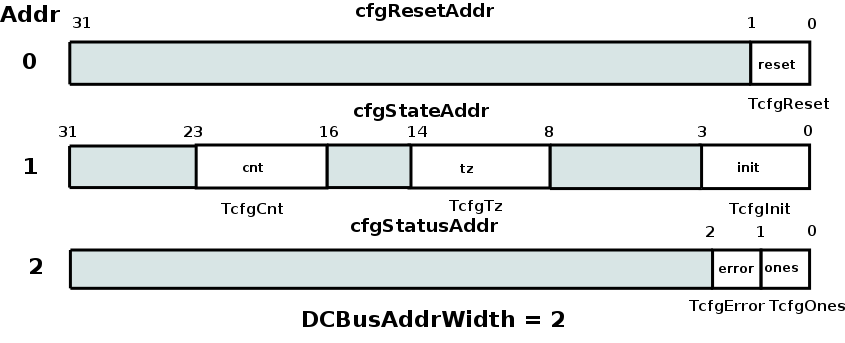
\includegraphics[width = 5 in]{LibFig/cbus1}
\caption{CBus Registers used in Block example}
\label{cbusreg}
\end{center}
\end{figure}

\begin{verbatim}
import CBus::*;       // this is a BSC library
import CfgDefines::*; // user defines - address,registers, etc

interface Block;
   // TODO: normally this block would have at least a few methods
   // Cbus interface is hidden, but it is there
endinterface

// In order to access the CBus at this parent, we need to expose the bus.   
// Only modules of type [Module] can be synthesized.
module [Module] mkBlock(IWithCBus#(DCBus, Block));
   let ifc <- exposeCBusIFC( mkBlockInternal );
   return ifc;
endmodule

// Within this module the CBus looks like normal Registers.
// This module can't be synthesized directly.
// How these registers are combined into CBus registers is 
// defined in the CfgDefines package.

module [DModWithCBus] mkBlockInternal( Block );
   // all registers are read/write from the local block point of view
   // config register interface types can be
   //   mkCBRegR  -> read only from config bus
   //   mkCBRegRW -> read/write from config bus
   //   mkCBRegW  -> write only from config bus
   //   mkCBRegRC -> read from config bus, write is clear mode
   //                i.e. for each bit a 1 means clear, 0 means don't clear
   // reset bit is write only from config bus
   // we presume that you use this bit to fire some local rules, etc
   Reg#(TCfgReset)  reg_reset_reset    <- mkCBRegW(cfg_reset_reset,    0 /* init val */);

   Reg#(TCfgInit)   reg_setup_init     <- mkCBRegRW(cfg_setup_init,    0 /* init val */);
   Reg#(TCfgTz)     reg_setup_tz       <- mkCBRegRW(cfg_setup_tz,      0 /* init val */);
   Reg#(TCfgCnt)    reg_setup_cnt      <- mkCBRegRW(cfg_setup_cnt,     1 /* init val */);

   Reg#(TCfgOnes)   reg_status_ones    <- mkCBRegRC(cfg_status_ones,   0 /* init val */);
   Reg#(TCfgError)  reg_status_error   <- mkCBRegRC(cfg_status_error,  0 /* init val */);

   // USER: you know have registers, so do whatever it is you do with registers :)
   // for instance
   rule bumpCounter ( reg_setup_cnt != unpack('1) );
      reg_setup_cnt <= reg_setup_cnt + 1;
   endrule

   rule watch4ones ( reg_setup_cnt == unpack('1) );
      reg_status_ones <= 1;
   endrule
endmodule
\end{verbatim}

The \te{CfgDefines} package contains the user defines describing how
the local registers are combined into the configuration bus.
\begin{verbatim}
package CfgDefines;
import CBus::*;

////////////////////////////////////////////////////////////////////////////////
/// basic defines
////////////////////////////////////////////////////////////////////////////////
// width of the address bus, it's easiest to use only the width of the bits needed
// but you may have other reasons for passing more bits around (even if some address
// bits are always 0)
typedef  2 DCBusAddrWidth;  // roof( log2( number_of_config_registers ) )

// the data bus width is probably defined in your spec
typedef 32 DCBusDataWidth;  // how wide is the data bus

////////////////////////////////////////////////////////////////////////////////
// Define the CBus
////////////////////////////////////////////////////////////////////////////////
typedef CBus#(  DCBusAddrWidth,DCBusDataWidth)          DCBus;
typedef CRAddr#(DCBusAddrWidth,DCBusDataWidth)          DCAddr;
typedef ModWithCBus#(DCBusAddrWidth, DCBusDataWidth, i) DModWithCBus#(type i);

////////////////////////////////////////////////////////////////////////////////
/// Configuration Register Types
////////////////////////////////////////////////////////////////////////////////
// these are configuration register from your design.  The basic
// idea is that you want to define types for each individual field
// and later on we specify which address and what offset bits these
// go to.  This means that config register address fields can 
// actually be split across modules if need be.
//
typedef bit      TCfgReset;

typedef Bit#(4)  TCfgInit;
typedef Bit#(6)  TCfgTz;
typedef UInt#(8) TCfgCnt;

typedef bit      TCfgOnes;
typedef bit      TCfgError;

////////////////////////////////////////////////////////////////////////////////
/// configuration bus addresses
////////////////////////////////////////////////////////////////////////////////
Bit#(DCBusAddrWidth) cfgResetAddr  = 0; // 
Bit#(DCBusAddrWidth) cfgStateAddr  = 1; // 
Bit#(DCBusAddrWidth) cfgStatusAddr = 2; // maybe you really want this to be 0,4,8 ???

////////////////////////////////////////////////////////////////////////////////
/// Configuration Register Locations
////////////////////////////////////////////////////////////////////////////////
// DCAddr is a structure with two fields
//     DCBusAddrWidth a ; // this is the address
//                        // this does a pure comparison
//     Bit#(n)        o ; // this is the offset that this register
//                        // starts reading and writting at

DCAddr cfg_reset_reset  = DCAddr {a: cfgResetAddr, o:  0};  // bits 0:0

DCAddr cfg_setup_init   = DCAddr {a: cfgStateAddr, o:  0};  // bits 0:0
DCAddr cfg_setup_tz     = DCAddr {a: cfgStateAddr, o:  4};  // bits 9:4
DCAddr cfg_setup_cnt    = DCAddr {a: cfgStateAddr, o: 16};  // bits 24:16

DCAddr cfg_status_ones  = DCAddr {a: cfgStatusAddr, o:  0};  // bits 0:0
DCAddr cfg_status_error = DCAddr {a: cfgStatusAddr, o:  1};  // bits 1:1

////////////////////////////////////////////////////////////////////////////////
///
////////////////////////////////////////////////////////////////////////////////
endpackage
\end{verbatim}

The \te{Tb} package executes the block.

\begin{verbatim}
import CBus::*;        // bsc library
import CfgDefines::*;  // address defines, etc
import Block::*;       // test block with cfg bus
import StmtFSM::*;     // just for creating a test sequence

(* synthesize *)
module mkTb ();
   // In order to access this cfg bus we need to use IWithCBus type
   IWithCBus#(DCBus,Block) dut <- mkBlock;
   
   Stmt test =
   seq
      // write the bits need to the proper address
      // generally this comes from software or some other packing scheme
      // you can, of course, create functions to pack up several fields
      // and drive that to bits of the correct width
      // For that matter, you could have your own shadow config registers
      // up here in the testbench to do the packing and unpacking for you
      dut.cbus_ifc.write( cfgResetAddr, unpack('1) );

      // put some ones in the status bits
      dut.cbus_ifc.write( cfgStateAddr, unpack('1) );
      
      // show that only the valid bits get written
      $display("TOP: state = %x at ", dut.cbus_ifc.read( cfgStateAddr ), $time);

      // clear out the bits
      dut.cbus_ifc.write( cfgStateAddr, 0 );

      // but the 'ones' bit was set when it saw all ones on the count
      // so read it to see that...
      $display("TOP: status = %x at ", dut.cbus_ifc.read( cfgStatusAddr ), $time);

      // now clear it
      dut.cbus_ifc.write( cfgStatusAddr, 1 );

      // see that it's clear
      $display("TOP: status = %x at ", dut.cbus_ifc.read( cfgStatusAddr ), $time);

      // and if we had other interface methods, that where not part of CBUS
      // we would access them via dut.device_ifc 
   endseq;
   mkAutoFSM( test );
endmodule
\end{verbatim}



\subsubsection{HList}

\label{sec-HList}
\index{HList (package)}

{\bf Package}

\begin{verbatim}
import HList :: * ;
\end{verbatim}


{\bf Description}

The \te{HList} package defines a datatype \te{HList} which 
stores a list of data of different types.   
The  package also provides typeclasses and functions to perform
various list  operations on the \te{HList} type.

The primitive data structures for an \te{HList} are \te{HNil}  and the
polymorphic \te{HCons}.  The various functions are provided by
typeclasses, one for each function.   

The package defines  a typeclass
\te{Gettable} for finding (\te{getIt}) and replacing (\te{putIt}) items in
an \te{HList}.  This requires that all the items in the \te{HList} are
different types.  If two types are the same, they must be
disambiguated by encapsulating at least one of them (but preferably
each of them) in a new struct type.  The functions of the
\te{Gettable} typeclass require that the \te{HList} be flat (no nested
\te{HLists}) and well-formed (terminating in \te{HNil}).  That is, the
target of a recursive search must be either the complete \te{hHead} or
found within the \te{hTail}.  

{\bf Types and type classes}


The \te{HList} packages defines a typeclass \te{HList}:

\begin{verbatim}
typeclass HList#(type l); 
\end{verbatim} 


The \te{HNil} datatype defines a nil instance, the empty set.  An
\te{HList} is usually terminated by a \te{HNil}.

\begin{verbatim}
typedef struct {} HNil deriving (Eq);
\end{verbatim}

The \te{HCons} datatype is a structure with two members, a head of
datatype \te{e} and a tail of datatype \te{l}.  

\begin{verbatim}
typedef struct {
   e hd;
   l tl;
   } HCons#(type e, type l) deriving (Eq);
\end{verbatim}


{\bf Functions}

The various functions for heterogenous lists are provided by
typeclasses, one for each functions.  


\index{HHead@\te{HHead} (typeclass)}
\index[function]{HList!HHead}

\begin{tabular}{|p{1 in}|p{4.5 in}|}
\hline
& \\
\te{HHead} & Returns the first element of the list.\\
\cline{2-2}
&\begin{libverbatim}
typeclass HHead#(type l, type h)
   dependencies (l determines h);
   function h hHead(l x);
endtypeclass

instance  HHead#(HCons#(e, l), e);
\end{libverbatim}
\\
\hline
\end{tabular}


\index{HTail@\te{HTail} (typeclass)}
\index[function]{HList!HTail}

\begin{tabular}{|p{1 in}|p{4.5 in}|}
\hline
& \\
\te{HTail} & Returns the tail element from the list.  \\
\cline{2-2}
&\begin{libverbatim}
typeclass HTail#(type l, type lt)
   dependencies (l determines lt);
   function lt hTail(l xs);
endtypeclass

instance HTail#(HCons#(e, l), l);
\end{libverbatim}
\\
\hline
\end{tabular}

\index{HLength@\te{HLength} (typeclass)}
\index[function]{HList!HLength}

\begin{tabular}{|p{1 in}|p{4.5 in}|}
\hline
& \\
\te{HLength} &Returns a numeric value with the length of the list.
For a \te{HNil}, will return 0.  \\
\cline{2-2}
&\begin{libverbatim}
typeclass HLength#(type l, numeric type n);
endtypeclass

instance HLength#(HNil, 0); 

instance HLength#(HCons#(e, l), nPlus1)
   provisos (HLength#(l, n), Add#(n,1,nPlus1));
\end{libverbatim}
\\
\hline
\end{tabular}




\index{HAppend@\te{HAppend} (typeclass)}
\index[function]{HList!HAppend}


\begin{tabular}{|p{1 in}|p{4.5 in}|}
\hline
& \\
\te{HAppend} & Appends two lists, returning the combined list.  The
elements do not have to be of the same data type.  The combined list
will be of type \te{l2}, and will contain all the elements of \te{xs}
followed in order by all the elements of \te{ys}.\\
\cline{2-2}
&\begin{libverbatim}
typeclass HAppend#(type l, type l1, type l2)
   dependencies ((l, l1) determines l2);
   function l2 hAppend(l xs, l1 ys);

instance HAppend#(HNil, l, l);

instance HAppend#(HCons#(e, l), l1, HCons#(e, l2))
   provisos (HList#(l), HAppend#(l, l1, l2));
\end{libverbatim}
\\
\hline
\end{tabular}


\index{HSplit@\te{HSplit} (typeclass)}
\index[function]{HList!hSplit}

\begin{tabular}{|p{1 in}|p{4.5 in}|}
\hline
& \\
\te{HSplit} & The \te{hSplit} function takes an \te{HList} of type
\te{l} and returns a \te{Tuple2} of two \te{HLists}.  This function is
the inverse of \te{hAppend}.\\
\cline{2-2}
&\begin{libverbatim}
typeclass HSplit#(type l, type l1, type l2);
   function Tuple2#(l1,l2) hSplit(l xs);
endtypeclass

instance HSplit#(HNil, HNil, HNil);

instance HSplit#(l, HNil, l);

instance HSplit#(HCons#(hd,tl), HCons#(hd,l3), l2)
   provisos (HSplit#(tl,l3,l2));
\end{libverbatim}
\\
\hline
\end{tabular}



\index{Gettable@\te{Gettable} (typeclass)}
\index[function]{HList!Gettable}

\begin{tabular}{|p{1 in}|p{4.5 in}|}
\hline
& \\
\te{Gettable} &This typeclass is for finding (\te{getIt}) and
replacing (\te{putIt}) a particular element in an \te{HList}. All items
in the \te{HList} must be of different types.  If two types are the
same, they should be disambiguated by encapsulating at least one of
them (and preferably both of them) in a new struct type.\\
\cline{2-2}
&\begin{libverbatim}
typeclass Gettable#(type c1, type c2);
   function c2 getIt(c1 x);
   function c1 putIt(c1 x, c2 y);
endtypeclass

instance Gettable#(HCons#(t1, t2), t1);

instance Gettable#(HCons#(t1, t2), t3)
   provisos (Gettable#(t2, t3));
\end{libverbatim}
\\
\hline
\end{tabular}

{\bf Small Lists}

The \te{HList} packcage provides type definitions for small lists, ranging
from 1 element to 8 elements, along with constructor functions to
build the lists.

{\bf HList1}
\begin{verbatim}
typedef HCons#(t, HNil)                                      
        HList1#(type t);

function HList1#(t1) hList1(t1 x1) = hCons(x1, hNil);  
\end{verbatim}

{\bf HList2}
\begin{verbatim}
typedef HCons#(t1, HCons#(t2, HNil))                         
        HList2#(type t1, type t2);

function HList2#(t1, t2) hList2(t1 x1, t2 x2) = hCons(x1, hCons(x2, hNil));  
\end{verbatim}

{\bf HList3}
\begin{verbatim}
typedef HCons#(t1, HCons#(t2, HCons#(t3, HNil)))             
        HList3#(type t1, type t2, type t3);

function HList3#(t1, t2, t3) hList3(t1 x1, t2 x2, t3 x3) 
      = hCons(x1, hCons(x2, hCons(x3, hNil)));
\end{verbatim}

{\bf HList4}
\begin{verbatim}
typedef HCons#(t1, HCons#(t2, HCons#(t3, HCons#(t4, HNil)))) 
        HList4#(type t1, type t2, type t3, type t4);

function HList4#(t1, t2, t3, t4) hList4(t1 x1, t2 x2, t3 x3, t4 x4)
      = hCons(x1, hCons(x2, hCons(x3, hCons(x4, hNil))));

\end{verbatim}

{\bf HList5}
\begin{verbatim}
typedef HCons#(t1, HCons#(t2, HCons#(t3, HCons#(t4, HCons#(t5, HNil)))))
        HList5#(type t1, type t2, type t3, type t4, type t5);

function HList5#(t1, t2, t3, t4, t5) hList5(t1 x1, t2 x2, t3 x3, t4 x4, t5 x5)
      = hCons(x1, hCons(x2, hCons(x3, hCons(x4, hCons(x5, hNil)))));
\end{verbatim}

{\bf HList6}
\begin{verbatim}
typedef HCons#(t1, HCons#(t2, HCons#(t3, HCons#(t4, HCons#(t5, HCons#(t6, HNil))))))
        HList6#(type t1, type t2, type t3, type t4, type t5, type t6);

function HList6#(t1, t2, t3, t4, t5, t6) 
   hList6(t1 x1, t2 x2, t3 x3, t4 x4, t5 x5, t6 x6)
      = hCons(x1, hCons(x2, hCons(x3, hCons(x4, hCons(x5, hCons(x6, hNil))))));
\end{verbatim}

{\bf HList7}
\begin{verbatim}
typedef HCons#(t1, HCons#(t2, HCons#(t3, HCons#(t4, HCons#(t5,
               HCons#(t6, HCons#(t7, HNil)))))))
        HList7#(type t1, type t2, type t3, type t4, type t5, type t6, type t7);

function HList7#(t1, t2, t3, t4, t5, t6, t7)
   hList7(t1 x1, t2 x2, t3 x3, t4 x4, t5 x5, t6 x6, t7 x7)
      = hCons(x1, hCons(x2, hCons(x3, hCons(x4, hCons(x5, hCons(x6, hCons(x7, hNil)))))));
\end{verbatim}

{\bf HList8}

\begin{verbatim}
typedef HCons#(t1, HCons#(t2, HCons#(t3, HCons#(t4, HCons#(t5, 
               HCons#(t6, HCons#(t7, HCons#(t8, HNil))))))))
        HList8#(type t1, type t2, type t3, type t4, type t5, type t6, type t7, type t8);

function HList8#(t1, t2, t3, t4, t5, t6, t7, t8)
   hList8(t1 x1, t2 x2, t3 x3, t4 x4, t5 x5, t6 x6, t7 x7, t8 x8)
      = hCons(x1, hCons(x2, hCons(x3, hCons(x4, hCons(x5, hCons(x6, 
              hCons(x7, hCons(x8, hNil))))))));
\end{verbatim}




\subsubsection{UnitAppendList}

\label{sec-UnitAppendList}
\index{UnitAppendList (package)}

{\bf Package}

\begin{verbatim}
import UnitAppendList :: * ;
\end{verbatim}


{\bf Description}


This provides a representation of lists for which append(x,y) is O(1), rather
than O(length(x)) as in the normal representation; the downside is that there
is no longer a unique representation for a given list.  These lists are useful
for situations in which the list is constructed by recursively amalgamating
lists from sub-computations, and then subsequently processed.
Functions for \te{map} and \te{mapM} are provided for processing
sublists during construction. 
For final processing it is almost always preferable first to flatten the list
(by a function also provided) into the conventional representation, thus
eliminating empty subtrees.


{\bf Types and type classes}

The \te{UnitAppendList} package defines the structure \te{UAList}:

\begin{verbatim}
typedef union tagged {
    void NoItems;
    a One;
    Tuple2#(UAList#(a),UAList#(a)) Append;
} UAList#(type a);
\end{verbatim} 

\te{UAList} is a member of the \te{DefaultValue} typeclass, which
    defines a default value for user defined structures.  The default
    value for \te{UAList} is defined as:

\begin{verbatim}
instance DefaultValue#(UAList#(a));
   defaultValue = NoItems;
endinstance
\end{verbatim}

{\bf Functions}

\index{flatten0@\te{flatten0} (function)}
\index[function]{UnitAppendList!flatten0}

\begin{tabular}{|p{.75 in}|p{5 in}|}
\hline
& \\
\te{flatten0} &Given a \te{UAList\#(a)} and a \te{List\#(a)}, returns
a conventional list of type \te{List}.\\
\cline{2-2}
& \begin{libverbatim}
function List#(a) flatten0(UAList#(a) c, List#(a) xs);
\end{libverbatim}
\\
\hline
\end{tabular}


\index{flatten@\te{flatten} (function)}
\index[function]{UnitAppendList!flatten}

\begin{tabular}{|p{.75 in}|p{5 in}|}
\hline
\te{flatten} & Converts a list of type \te{UAList} into a conventional
list of type \te{List}.\\
\cline{2-2}
& \begin{libverbatim}
function List#(a) flatten(UAList#(a) c) = flatten0(c, Nil);
\end{libverbatim}
\\
\hline
\end{tabular}

\index{uaMap@\te{uaMap} (function)}
\index[function]{UnitAppendList!uaMap}

\begin{tabular}{|p{.75 in}|p{5 in}|}
\hline
& \\
\te{uaMap} &Maps a function of a list of type \te{UAList}, returning a
\te{UAList}.\\
\cline{2-2}
& \begin{libverbatim}
function UAList#(b) uaMap(function b f(a x), UAList#(a) c);
\end{libverbatim}
\\
\hline
\end{tabular}


\index{uaMapM@\te{uaMapM} (function)}
\index[function]{UnitAppendList!uaMapM}


\begin{tabular}{|p{.75 in}|p{5 in}|}
\hline
& \\
\te{uaMapM} & Maps a monadic function of a list of type \te{UAList}, returning a
\te{UAList}.\\
\cline{2-2}
& \begin{libverbatim}
module uaMapM#(function module#(b) f(a x), UAList#(a) c)(UAList#(b));
\end{libverbatim}
\\
\hline
\end{tabular}


% ------------------------------------------------------------

% The one reference (in LibDoc/Prelude.tex) is given instead
% as a footnote, rather than far removed in a References
% section at the end.

%\clearpage
%\bibliography{libraries_ref_guide}
%\bibliographystyle{alpha}
%\addcontentsline{toc}{section}{References}

% ------------------------------------------------------------

\clearpage
\phantomsection
\addcontentsline{toc}{section}{Index}
\printindex

% ------------------------------------------------------------

\clearpage
\phantomsection
\addcontentsline{toc}{section}{Function and Module by Package}
\printindex[function]

% ------------------------------------------------------------

\clearpage
\phantomsection
\addcontentsline{toc}{section}{Typeclasses}
\printindex[typeclass]

% ------------------------------------------------------------

\end{document}
